\documentclass[11pt,a4paper]{article}
\usepackage[T1]{fontenc}
\usepackage[utf8]{inputenc}
\usepackage{lmodern,microtype}
\usepackage[a4paper,margin=25mm,headheight=14pt]{geometry}
\usepackage{amsmath,amssymb,amsthm,mathtools,mathrsfs}
\usepackage{booktabs,longtable,array,enumitem,xcolor,fancyhdr}
\usepackage{tikz}
\usepackage[hyphens]{url}
\usepackage[colorlinks=true,linkcolor=blue!45!black,citecolor=blue!45!black,urlcolor=blue!45!black]{hyperref}
\usepackage{bookmark}
\newtheorem{theorem}{Theorem}[section]
\newtheorem{lemma}[theorem]{Lemma}
\newtheorem{proposition}[theorem]{Proposition}
\newtheorem{corollary}[theorem]{Corollary}
\theoremstyle{definition}
\newtheorem{definition}[theorem]{Definition}
\newtheorem{example}[theorem]{Example}
\theoremstyle{remark}
\newtheorem{remark}[theorem]{Remark}
\newcommand{\Q}{\mathbb Q}
\newcommand{\R}{\mathbb R}
\newcommand{\C}{\mathbb C}
\newcommand{\N}{\mathbb N}
\newcommand{\Z}{\mathbb Z}
\newcommand{\Qbar}{\overline{\mathbb Q}}
\newcommand{\E}{\mathbb E}
\newcommand{\PP}{\mathbb P}
\DeclareMathOperator{\tr}{tr}
\DeclareMathOperator{\rank}{rank}
\DeclareMathOperator{\supp}{supp}
\DeclareMathOperator{\diag}{diag}
\DeclareMathOperator{\ord}{ord}
\DeclareMathOperator{\Var}{Var}
\DeclareMathOperator{\Cov}{Cov}
\DeclareMathOperator{\Repart}{Re}
\DeclareMathOperator{\CT}{CT}
\numberwithin{equation}{section}
\setlength{\emergencystretch}{3em}
\setlength{\parskip}{3pt}
\allowdisplaybreaks[2]
\setcounter{tocdepth}{1}
\pagestyle{fancy}\fancyhf{}
\fancyhead[L]{\small KEIO}
\fancyhead[R]{\small Proof transfers and global classifications}
\fancyfoot[C]{\thepage}

\hypersetup{pdftitle={Proof Transfers and Global Classifications: Collected Research Manuscripts},pdfauthor={KEIO}}
\makeatletter
\renewcommand*\l@section{\@dottedtocline{1}{0em}{4.7em}}
\makeatother
\newcommand{\collectedpart}[1]{%
 \clearpage\part{#1}%
 \setcounter{section}{0}%
 \renewcommand{\thesection}{\Roman{part}.\arabic{section}}%
 \renewcommand{\theHsection}{p\arabic{part}.s\arabic{section}}%
 \renewcommand{\arraystretch}{1}%
}
\newcommand{\collectedappendix}{%
 \setcounter{section}{0}%
 \renewcommand{\thesection}{\Roman{part}.\Alph{section}}%
 \renewcommand{\theHsection}{p\arabic{part}.a\arabic{section}}%
}

\begin{document}

\title{Proof Transfers and Global Classifications\\[6pt]
\large Collected Research Manuscripts\\
Spectral Design, Statistical Recovery, Recurrences,\\
Period Geometry, and Arithmetic}
\author{KEIO}
\date{19 October 2026}
\maketitle
\begin{abstract}
This volume brings together the eight research manuscripts developed in
the present research sequence. The collection begins with transfers to
exact recurrence complexity, random-matrix statistics, spectral network
design, Hamiltonian dynamics, stopping boundaries, and hidden-state
recovery. It continues through entropy--transport methods for mixture
likelihood, complete support and noise regimes, and sharp graph-design
comparisons. The differential and arithmetic parts study weighted Franel
series, anisotropic lattice and banana periods, differential Galois groups,
algebraic quantiles, arithmetic subsequences, and Ap\'ery limits.
The final part contains the expanded entropy--transport and
Laplace-monodromy manuscript, including optimal coefficient exponents,
complete testing transitions, Bessel determinant modules, tableau values,
and split-beta orthogonality.
All eight mathematical texts are retained with their proofs, examples,
limitations, and supporting appendices. A single notation framework,
part-qualified cross-references, a unified bibliography, and an editorial
map make the progression of results explicit. Earlier special cases and
alternative arguments remain available for comparison; statements of
open directions in those earlier texts are interpreted with the later
closures indicated in this volume.
\end{abstract}

\noindent\textbf{Research status.} This is a consolidated research draft
prepared with AI assistance. Its component manuscripts underwent the
internal checks described in their texts; compilation and integration
checks do not constitute external mathematical peer review. Historical
priority and publication-level significance are not certified by this
collection.
\clearpage
\section*{Editorial guide and coverage}
\addcontentsline{toc}{section}{Editorial guide and coverage}

The scope of the collection is the eight manuscripts produced during this
research sequence, including the most recent expanded revision. The older
numbered manuscripts supplied as methodological source material remain
bibliographical sources, rather than additional constituent papers.
Each part preserves the mathematical body of one manuscript. Repeated
supporting proofs have deliberately been retained where they make a part
self-contained or document a different argument. Duplicate front matter
and repeated reference lists are consolidated.

\begin{center}\small
\begin{tabular}{@{}>{\raggedright\arraybackslash}p{.07\textwidth}>{\raggedright\arraybackslash}p{.47\textwidth}>{\raggedright\arraybackslash}p{.37\textwidth}@{}}
\toprule
Part & Constituent manuscript & Main coverage\\
\midrule
I & Exact Complexity and Arithmetic Transfers & Six transfers, from lattice moments and Jacobi ensembles to clocks, stopping, and hidden-state recovery.\\[5pt]
II & Sharp Bounds and Connection Formulas Beyond Existing Restrictions & Trees, alternating binomial sums, nonresonant trace connections, and long hidden trajectories.\\[5pt]
III & Entropy, Likelihood Geometry, and Sharp Proof Transfers & Corrupted reports, unequal depths, posterior transport, all connected graphs, and phase weights.\\[5pt]
IV & Global Parameter Theorems from Entropy, Transport, and Spectral Structure & All-support Poisson recovery, resonant trace connections, block graphs, and a robustness obstruction.\\[5pt]
V & Global Algebraicity and Exact Complexity & Weighted Franel algebraicity, hypercubic rank, quantiles, Gaussian likelihood, and graph inflation.\\[5pt]
VI & Global Galois Groups and Complete Parameter Classifications & Galois groups, colliding thresholds, half-integer quantiles, cubic weights, and all-scale Gaussian recovery.\\[5pt]
VII & Beyond Generic Parameters: Global Classifications & Remaining orthogonal groups, all-exponent recurrence widths, complementary beta quantiles, and a noisy-observation obstruction.\\[5pt]
VIII & Entropy--Transport, Critical Values, and Laplace Monodromy & The latest expanded manuscript: coefficient optimality, statistical transitions, subsequences, local Fourier bounds, and arithmetic classifications.\\
\bottomrule
\end{tabular}
\end{center}

Part-qualified numbering makes every theorem, equation, and appendix
reference unambiguous. For example, a reference beginning with VIII belongs
to the final manuscript; appendix letters remain local to their part.
Each part starts with its original abstract and an integration note.
All cited reference entries are collected at the end. The accompanying
TEX source contains the full volume and requires no external manuscript,
bibliography database, image, or included source file.

\subsection*{How to read the successive closures}

The chapter sequence records research development, so a statement such as
``not proved here'' in an earlier part describes that part's argument.
It must be read together with the following developments. The nonresonant
Jacobi trace connection in Part II is continued to resonant parameters in
Part IV. The tree design result in Part II is followed by connected-graph,
block-graph, and dense-inflation comparisons. The all-support Poisson
theorem of Part IV is incorporated with its proof into Part VIII.
The support-free growing-support Gaussian result in Part V is complemented
by a known-support all-scale theorem in Part VI. These use different
optimization domains: Part VI also explains why the unrestricted fit
cannot adapt to arbitrarily small known intervals. The heteroscedastic
obstruction in Part VII concerns a different observation model.

The phase and cubic-weight recurrence classifications in Parts III and VI
are followed by the all-exponent, all-weight result in Part VII and the
arithmetic-subsequence theorem in Part VIII. Differential Galois groups
left open by the rank argument in Part V are addressed in Parts VI and VII.
Part VIII gives the local Fourier formulation used to repair the
Laplace--Jordan argument and states its regularity hypotheses explicitly.
The precise replacement is Theorem~\ref{p8:ljr:borel}; the complete
subsequence classification is Theorem~\ref{p8:ac:subsequence}.
All algebraicity and transcendence statements retain the precise
parameter assumptions and exceptions in their individual theorems.

Minimum recurrence width is not the number of nonzero recurrence terms.
The sparse-term lower bounds for alternating and unit-circle weights in
Parts II and III therefore remain additional assertions, with their own
positivity and Descartes arguments. They are not replaced by the later
width-only classifications, even when those later results cover more
weights or more subsequences.

The latest part does not supersede the collection's unrelated results in
network optimization, Hamiltonian arithmetic, optimal stopping, hidden
trajectories, robust likelihood, or Jacobi trace connections. Those
arguments are therefore retained in full. No new theorem is claimed merely
from placing the manuscripts in a single volume.

\clearpage
\begingroup\small
\tableofcontents
\endgroup
\clearpage


\collectedpart{Exact Complexity and Arithmetic Transfers}\label{part:1}

\begin{abstract}
We transfer proof mechanisms from recurrence minimality, period arithmetic,
weighted Laplacian spectra, and mixture identification to six concrete
problems. Products of separated central-trinomial moments have exact
recurrence width $\prod_i(m_i+1)$. Jacobi transforms have exact differential
order $N+1$, increasing to $2^N$ under arbitrarily small separated weights
at even nonnegative Dyson index. For every inverse-power spectral loss,
we determine the unique optimal conductances when a matching of links is
forbidden. Holomorphic time differentials imply simultaneous
transcendence of Hamiltonian coordinates at nonzero algebraic-logarithmic
clock times and a harmonic exception for action-quantized energies.
For a mean-reverting square-root diffusion, we verify power-call stopping
for every positive real power, classify algebraic exercise boundaries by
an exact discount resonance, and prove transcendence of zero-state values
at positive integer discount ratios. Finally, a known emission family with
finite-dimensional mixing defect admits hidden-population recovery from
three visits despite unknown persistence; an explicit positive analytic
family shows both the failure of two visits and the sharp risk
$\Theta(\min\{1,(r^2\sqrt{N})^{-1}\})$ on a specified submodel.
The proofs identify the assumptions and classical inputs of each transfer.
\end{abstract}

\noindent\textbf{Integration note.} This opening manuscript supplies six distinct transfers. Its methodological sources are the older numbered manuscripts cited in its introduction. The nonlinear clock, stopping, spectral-design, and hidden-state results are retained here in full.
\clearpage

\section{What is transferred, and what is proved}
The starting collection contains several distinct kinds of proof: positive
integrals make singularities visible; a finite-dimensional representation
gives an upper bound that can be matched by those singularities; an exact
spectral region converts inverse existence into optimization; and arithmetic
separation of Abelian integrals from logarithms constrains dynamical motion.
A separate observation-theoretic principle distinguishes local differential
relations from the kernel of a global mixing operator. We use these mechanisms
as starting points, and reconstruct the needed arguments for the target
problems below.

There are three different senses of an exact conclusion in this paper.
A \emph{complexity theorem} supplies matching upper and lower bounds.
A \emph{classification theorem} states the exceptional parameter set as well
as the generic alternative. An \emph{observation theorem} proves both a
sufficient experiment and an obstruction to a smaller or noisier one.
These claims must not be conflated with historical priority.

The target problems are deliberately concrete. They ask for a minimal
recurrence for products of central-trinomial moments, the change in
Jacobi-trace differential complexity when weights are separated, an optimal
weighted network when several links are forbidden, arithmetic constraints
on polynomial Hamiltonian motion, the optimal exercise boundary of a
mean-reverting diffusion, and recovery of a hidden population with unknown
temporal persistence. The problem definitions are part of the statements;
none of the conclusions is obtained merely by relabelling a constant from
the source collection.

Classical inputs include Selberg and Kummer identities, analytic subgroup
and $E$-function theorems, finite-dimensional linear algebra, and elementary
statistical testing. Whenever a result relies on such an input, it is stated
at the point of use. In the mechanical application, action quantization
defines semiclassical levels; the exact quantum spectrum is a separate
problem.


The source methods were selected from the supplied manuscripts
\cite{p1:Keio006transfer,p1:Keio015transfer,p5:Keio024,p1:Keio025transfer,p1:Keio028transfer,p4:Keio029,p1:Keio030transfer,p5:Keio032}.
Their role is methodological provenance; the target results below include
their own arguments and identify any external theorem they use.
\begin{center}
\small
\begin{tabular}{@{}>{\raggedright\arraybackslash}p{.27\textwidth}>{\raggedright\arraybackslash}p{.30\textwidth}>{\raggedright\arraybackslash}p{.34\textwidth}@{}}
\toprule
Mechanism & Target field & Conclusion proved\\
\midrule
Visible critical values and tensor bounds & Lattice return probabilities & Exact shift width, including repeated parameters\\
Distinct endpoint phases & Random-matrix linear statistics & Exact differential order and a symmetry-breaking jump\\
Spectral feasibility and strict convexity & Network design & Unique optimum for every inverse-power loss\\
Holomorphic time forms & Classical and semiclassical mechanics & Arithmetic clocks and exceptional quantization levels\\
$E$-function specialization & Mean-reverting optimal stopping & Discount-resonance classification of a genuine exercise boundary\\
Mixture-kernel repair and temporal moments & Hidden-state statistics & Minimal observation count and persistence-dependent minimax rate\\
\bottomrule
\end{tabular}
\end{center}
\clearpage


\section{Exact recurrence widths for anisotropic return probabilities}
\label{p1:sec:transfer-recurrences}

\subsection{A transfer from critical values to Hadamard products}

The singularity-counting argument for Franel sequences has an application
to products of classical moment sequences and to return probabilities of
finite-range random walks.  It determines an exact recurrence width in every
dimension, including all positive integer multiplicities of the parameters.
The result is not presented as the resolution of a separately named published
conjecture: the literature checked below does not supply such a conjecture for
this family.  Its contribution here is a uniform, explicit lower bound matching
the standard symmetric-power upper bound.

For real numbers $p>1$ define
\begin{equation}\label{p1:eq:transfer-Lp}
 L_p(x)=(p-1)+\frac{p+1}{2}(x+x^{-1}),\qquad
 u_p(n)=\operatorname{CT}_x L_p(x)^n \quad(n\geq0).
\end{equation}
The generalized central trinomial coefficient is
\[
 T_n(b,c)=\sum_{j=0}^{\lfloor n/2\rfloor}
 \binom n{2j}\binom{2j}j b^{n-2j}c^j.
\]
Thus $u_p(n)=T_n(p-1,(p+1)^2/4)$.  In particular $u_p(n)$ is a
positive integer when $p$ is an odd positive integer.  The generating
function and three-term recurrence are classical; see
\cite{p1:Noe2006transfer,p1:LWW2023transfer}.  For completeness the special
case needed here will be derived below.

Fix $s\geq1$, distinct odd primes $p_1,\ldots,p_s$, and integers
$m_1,\ldots,m_s\geq1$.  Put
\begin{equation}\label{p1:eq:transfer-An}
 D=\sum_{i=1}^s m_i,\qquad N=\prod_{i=1}^s(m_i+1),\qquad
 A_n=\prod_{i=1}^s u_{p_i}(n)^{m_i}.
\end{equation}
A recurrence of shift width $r$ means an identity
\[
 \sum_{j=0}^r q_j(n)A_{n+j}=0,
 \qquad q_j\in\mathbb C(n),\quad q_0q_r\ne0,
\]
valid for all sufficiently large integers $n$.  No degree bound is imposed
on its rational coefficients.

\begin{theorem}[Exact product width]\label{p1:thm:transfer-exact-width}
For the sequence in \eqref{p1:eq:transfer-An}, the least recurrence width
over $\mathbb C(n)$ is exactly
\[
 \boxed{\prod_{i=1}^s(m_i+1).}
\]
A recurrence of this width exists over $\mathbb Q(n)$.  The same conclusion
holds for multiplicatively independent rational parameters $p_i>1$, without
the assertion that every $A_n$ is an integer.
\end{theorem}

The conclusion measures the width in the discrete variable $n$.  It is not
a claim about the minimum differential order of the generating function.
Repeated parameters contribute $m_i+1$, whereas distinct independent
parameters contribute multiplicatively.  In particular the width can be
$2^D$ even though the underlying Laurent polynomial has degree at most one
in each individual variable.

\subsection{Visibility and the recurrence budget}

We recall the precise analytic principle, including the condition that
prevents cancellation on an interior critical fiber.

\begin{lemma}[Definite-fiber visibility]\label{p1:lem:transfer-visibility}
Let $M$ be a compact real-analytic manifold of positive dimension $d$ with
a positive analytic density $d\mu$, and let $\Phi:M\to\mathbb R$ be
analytic.  Suppose $v\ne0$ is a critical value whose critical fiber contains
finitely many critical points, all nondegenerate and all local maxima, or
all nondegenerate and all local minima.  Regular points on the same fiber
are allowed.  If
\[
 a_n=\int_M\Phi^n\,d\mu,\qquad F(t)=\sum_{n\geq0}a_nt^n,
\]
then a branch continued from the germ of $F$ at $0$ is singular at $t=1/v$.
Consequently every rational-coefficient recurrence for $(a_n)$ has width
at least the number of distinct nonzero values with this property.
\end{lemma}

\begin{proof}
The analytic Morse lemma and polar coordinates show that the pushforward
$\Phi_*\mu$ has, near $v$, density
\[
 \rho(v+x)=r(x)+\boldsymbol1_{\{\epsilon x>0\}}
 |x|^{d/2-1}h(|x|),\qquad h(0)>0,
\]
where $r$ is smooth and $h$ is analytic.  Here $\epsilon=1$ at minima and
$\epsilon=-1$ at maxima.  To justify this with regular points on the fiber,
take disjoint Morse neighborhoods and cutoffs equal to one near each critical
point.  The complement is a compact submersion region over a sufficiently
small interval about $v$, whose pushforward is smooth.  Inside a Morse chart,
the density contribution at distance $w>0$ from $v$ is
\[
 \frac12w^{d/2-1}\int_{\mathbb S^{d-1}}g(\sqrt w\,\omega)\,d\omega.
\]
The spherical average is analytic in $w$, with positive constant term.
Every critical point contributes on the same side, so the leading
coefficients add.  The resulting one-sided term is not smooth, for either
integer or half-integer exponent, and cannot be canceled by $r$.

The Cauchy transform
\[
 G(z)=\int_M\frac{d\mu(x)}{z-\Phi(x)}
\]
is holomorphic in the upper half-plane and satisfies
$G(z)=z^{-1}F(z^{-1})$ near infinity.  Its boundary distribution obeys
$-\pi^{-1}\operatorname{Im}G(x+i0)=\Phi_*\mu$ by the Poisson kernel.
If this branch extended holomorphically through $v$, its imaginary part on
the real axis would be analytic, contradicting the nonsmooth density.
Inversion gives the asserted singularity of the continued germ of $F$.

For the last assertion clear the denominators of a width-$r$ recurrence,
writing its coefficients as $q_j(n)\in\mathbb C[n]$.  With
$\vartheta=t\,d/dt$, summation gives
\[
 \left(\sum_{j=0}^r t^{r-j}q_j(\vartheta-j)\right)F(t)=R(t),
\]
where $R$ is a polynomial of initial terms.  If
$e=\max_j\deg q_j$ and $c_j=[n^e]q_j(n)$, the coefficient of the
highest ordinary derivative is $t^eH(t)$, with
\[
 H(t)=\sum_{j=0}^r c_jt^{r-j}\ne0,\qquad \deg H\leq r.
\]
An ordinary point of this inhomogeneous linear differential equation cannot
be a singularity of any continued solution branch.  Thus every nonzero
finite singularity just obtained is a zero of $H$, proving the bound.
\end{proof}

\subsection{All nonzero critical fibers are definite}

Use one angle $\theta_{i,j}$ for each pair $1\leq i\leq s$,
$1\leq j\leq m_i$, and normalized Haar measure on $\mathbb T^D$.
Constant-term extraction gives
\begin{equation}\label{p1:eq:transfer-Phi}
 A_n=\int_{\mathbb T^D}\Phi(\theta)^n\,d\theta,\qquad
 \Phi(\theta)=\prod_{i=1}^s\prod_{j=1}^{m_i}
 \bigl((p_i-1)+(p_i+1)\cos\theta_{i,j}\bigr).
\end{equation}
The convention in the integral includes normalization by $(2\pi)^{-D}$.

\begin{lemma}[The complete critical-value list]
\label{p1:lem:transfer-corners}
All critical points with $\Phi\ne0$ have every angle equal to $0$ or $\pi$.
For $k_i$ angles equal to $0$ in block $i$, their value is
\begin{equation}\label{p1:eq:transfer-values}
 v_{\boldsymbol k}=2^D(-1)^{D-\sum_i k_i}
                    \prod_{i=1}^s p_i^{k_i},
 \qquad 0\leq k_i\leq m_i.
\end{equation}
These $N$ values are distinct.  Every critical point over a positive
$v_{\boldsymbol k}$ is a nondegenerate maximum, and every one over a
negative $v_{\boldsymbol k}$ is a nondegenerate minimum.
\end{lemma}

\begin{proof}
At a nonzero value no factor in \eqref{p1:eq:transfer-Phi} vanishes.
The logarithmic derivative with respect to $\theta_{i,j}$ is
\[
 -\frac{(p_i+1)\sin\theta_{i,j}}
 {(p_i-1)+(p_i+1)\cos\theta_{i,j}}.
\]
It vanishes exactly when $\theta_{i,j}\in\{0,\pi\}$.
The corresponding factor values are $2p_i$ and $-2$, respectively,
giving \eqref{p1:eq:transfer-values}.  Unique factorization shows that
equality of two absolute values forces equality of every $k_i$.
Multiplicative independence gives the same argument for rational $p_i$.

At a corner, every off-diagonal Hessian entry is zero.  The diagonal entry
for angle $\theta_{i,j}$ is
\[
 -v_{\boldsymbol k}
 \frac{(p_i+1)\cos\theta_{i,j}}
 {(p_i-1)+(p_i+1)\cos\theta_{i,j}}.
\]
The quotient is $(p_i+1)/(2p_i)>0$ at $0$, and $(p_i+1)/2>0$
at $\pi$.  Thus all Hessian eigenvalues are nonzero and have sign
$-\operatorname{sgn}(v_{\boldsymbol k})$.  This also proves that all
critical points on any one nonzero fiber use the same side; their
contributions cannot cancel in Lemma~\ref{p1:lem:transfer-visibility}.
\end{proof}

The lemma and the visibility principle give a lower bound of $N$ over
$\mathbb C(n)$.  This argument does not require irreducibility of a
telescoper, numerical guessing, or noncancellation of complex saddle-point
expansions.

\subsection{A matching upper bound from symmetric powers}

The one-coordinate generating function is
\begin{equation}\label{p1:eq:transfer-one-GF}
 \sum_{n\geq0}u_p(n)t^n
 =\frac1{\sqrt{1-2(p-1)t-4pt^2}}.
\end{equation}
For example, integrate the geometric series for
$1/(1-t((p-1)+(p+1)\cos\theta))$; the constant-term binomial expansion
gives the same identity formally.  Differentiating
\eqref{p1:eq:transfer-one-GF} and comparing coefficients proves
\begin{equation}\label{p1:eq:transfer-3term}
 (n+1)u_p(n+1)=(2n+1)(p-1)u_p(n)+4pn\,u_p(n-1)
 \quad(n\geq1),
\end{equation}
with $u_p(0)=1$ and $u_p(1)=p-1$.

For a fixed exponent $m$, the $m+1$ monomials
\[
 u_p(n)^{m-j}u_p(n+1)^j,\qquad 0\leq j\leq m,
\]
form a vector whose shift is a rational matrix times the original vector:
replace $u_p(n+2)$ using \eqref{p1:eq:transfer-3term} and expand binomially.
For rational $p$ all matrix entries lie in $\mathbb Q(n)$.
Taking the tensor product of these symmetric-power systems over the
$s$ blocks gives an $N$-dimensional system containing $A_n$ as a coordinate.
The $N+1$ coordinate rows expressing $A_n,\ldots,A_{n+N}$ in terms of
the state at $n$ are linearly dependent over $\mathbb Q(n)$.  Consequently
$A_n$ satisfies a recurrence of width at most $N$, allowing finitely many
initial exceptions when rational denominators vanish.  Combined with the
lower bound already proved, this completes the proof of
Theorem~\ref{p1:thm:transfer-exact-width}.

\begin{corollary}[Powers of the usual central trinomial coefficients]
\label{p1:cor:transfer-trinomial-power}
Let $C_n=\operatorname{CT}_x(1+x+x^{-1})^n$.  For every integer $m\geq1$,
the least recurrence width of $C_n^m$ over $\mathbb C(n)$ is $m+1$.
\end{corollary}
\begin{proof}
For $p=3$, $L_3(x)=2(1+x+x^{-1})$ and $u_3(n)=2^nC_n$.
Multiplication of a sequence by a nonzero geometric sequence preserves
its minimum recurrence width: absorb the geometric factors into the
individual coefficients.  Apply the main theorem with one block.
\end{proof}

\subsection{Rigidity of the leading recurrence symbol}

\begin{theorem}[Exact singularity set and leading symbol]
\label{p1:thm:transfer-symbol}
Let $F(t)=\sum_{n\geq0}A_nt^n$ for \eqref{p1:eq:transfer-An}.  The set of
nonzero finite points at which some branch continued from the germ of $F$
is singular is exactly
\[
 \{v_{\boldsymbol k}^{-1}:0\leq k_i\leq m_i\}.
\]
For any width-$N$ polynomial-coefficient recurrence
$\sum_{j=0}^N q_j(n)A_{n+j}=0$, put
$e=\max_j\deg q_j$ and $c_j=[n^e]q_j(n)$.  There is a nonzero constant
$c$ such that
\begin{equation}\label{p1:eq:transfer-symbol}
 \sum_{j=0}^N c_jt^{N-j}
 =c\prod_{0\leq k_i\leq m_i}(1-v_{\boldsymbol k}t).
\end{equation}
\end{theorem}

\begin{proof}
The budget polynomial on the left is nonzero and has degree at most $N$.
The $N$ distinct reciprocal critical values are all zeros of it, by the
visibility lemma.  Its degree must therefore be exactly $N$, and these
are all its roots, proving \eqref{p1:eq:transfer-symbol}.  The associated
inhomogeneous differential equation is ordinary away from these points
and $0$, and therefore has no other nonzero finite singularities for
any branch of its solution $F$.  Visibility already proves the reverse
inclusion.
\end{proof}

This is an exact constraint on every recurrence of minimum width, including
ones with larger polynomial degrees than necessary.  It can be used to
reject an incorrectly guessed recurrence without first factoring its Ore
operator.  It also records every secondary exponential scale, although a
single dominant asymptotic ratio sees only
$2^D\prod_i p_i^{m_i}$.

\subsection{A completely explicit two-parameter certificate}

Take $p_1=3$, $p_2=5$, $m_1=m_2=1$.  Then
\[
 A_n=T_n(2,4)T_n(4,9)
 =1,8,408,15680,750880,36334848,1844830464,\ldots.
\]
The exact recurrence is
\begin{align}\label{p1:eq:transfer-example-rec}
0={}&57600(n+1)^2(2n+7)A_n\notag\\
 &-1920(2n+3)^2(2n+7)A_{n+1}\notag\\
 &-32(2n+5)(49n^2+245n+261)A_{n+2}\notag\\
 &-8(2n+3)(2n+7)^2A_{n+3}
 +(n+4)^2(2n+3)A_{n+4},\qquad n\geq0.
\end{align}
It has minimum width four, since the visible critical values are
$4,-12,-20,60$.  The leading-symbol identity is
\[
 115200t^4-15360t^3-3136t^2-64t+2
 =2(1-4t)(1+12t)(1+20t)(1-60t).
\]

Here is an exact algebraic certificate of the recurrence, independent of
checking initial values.  Set
\[
 M_p(n)=\begin{pmatrix}
 0&1\\[1mm]
 4p(n+1)/(n+2)&(p-1)(2n+3)/(n+2)
 \end{pmatrix},\qquad K(n)=M_3(n)\otimes M_5(n),
\]
and let $e_1=(1,0,0,0)$.  If $q_0,\ldots,q_4$ are the coefficients
displayed in \eqref{p1:eq:transfer-example-rec}, direct rational arithmetic
gives the row identity
\[
 q_0(n)e_1+
 \sum_{j=1}^4q_j(n)e_1K(n+j-1)\cdots K(n)=0.
\]
Multiplication by
$(u_3(n),u_3(n+1))^{\mathsf T}\otimes
 (u_5(n),u_5(n+1))^{\mathsf T}$ proves the recurrence.
The accompanying exact-arithmetic certificate verifies this rational
matrix identity; initial-term checks serve only as additional diagnostics.

\subsection{A Markov-chain interpretation}

Consider a discrete-time walk on $\mathbb Z^D$.  At each step all coordinate
increments are independent.  A coordinate in block $i$ has distribution
\begin{equation}\label{p1:eq:transfer-walk}
 \mathbb P(\Delta=0)=\frac{p_i-1}{2p_i},\qquad
 \mathbb P(\Delta=1)=\mathbb P(\Delta=-1)=\frac{p_i+1}{4p_i}.
\end{equation}
The step distribution has finite support, positive holding probability,
and positive probabilities for both signs in every coordinate.  Let
$R_n$ be its probability of returning to the origin after $n$ steps.

\begin{corollary}[Exact width of anisotropic return probabilities]
\label{p1:cor:transfer-walk}
For the walk \eqref{p1:eq:transfer-walk},
\[
 R_n=\frac{A_n}{(2^D\prod_i p_i^{m_i})^n},\qquad
 \operatorname{width}_{\mathbb C(n)}(R)=\prod_i(m_i+1).
\]
Consequently anisotropic walks with one coordinate for each of $D$
distinct odd primes have exact recurrence width $2^D$.  When all coordinates
have the same parameter, their exact width is $D+1$.
\end{corollary}

\begin{proof}
The one-coordinate probability generating Laurent polynomial is
$L_{p_i}(x)/(2p_i)$.  Independence, followed by constant-term extraction
for the origin, proves the formula for $R_n$.  A nonzero geometric
normalization preserves recurrence width, as in
Corollary~\ref{p1:cor:transfer-trinomial-power}.
\end{proof}

This return-probability statement is an application of the exact-width
theorem, not a second independent solution of an open problem.  The sharp
change from $D+1$ to $2^D$ quantifies how distinct coordinate parameters
remove the symmetric-power reduction.

\subsection{Literature boundary and remaining work}

Generalized central trinomial coefficients, their Legendre-polynomial
representations, moment properties, and three-term recurrence are classical;
the studies \cite{p1:Noe2006transfer,p1:LWW2023transfer} concern this established
family.  Closure under Hadamard products and the symmetric-power construction
are also standard.  The substantive assertion proved here is the matching
lower bound for the explicit independent-parameter family, together with
the complete nonzero finite singularity set and forced leading symbol.
The proof is self-contained once elementary analytic Morse theory and the
ordinary-point theorem for linear differential equations are available.

The wider methodological context is recurrence minimality.  Straub and
Zudilin \cite{p8:AC_SZ} explicitly distinguish minimum telescoping
order from minimum order among all rational-coefficient recurrences for
Franel sums.  The present lower bound addresses the latter notion for
a different family.  We do not claim that their Franel problem is newly
settled by this section, nor that any existing central-trinomial congruence
or real-rootedness question has been resolved here.  A more exhaustive
priority search for the exact product-width formula remains appropriate
before journal submission.  Multiplicatively dependent distinct parameters
can cause critical-value collisions; the proof still supplies a lower
bound equal to the number of distinct values, but does not assert a
complete minimum-width formula on those collision loci.


% Standalone section fragment. Requires amsmath, amssymb, amsthm.
% The theorem environments theorem, lemma, corollary, remark are assumed.
\section{Jacobi ensembles: exact differential complexity under symmetry breaking}
\label{p1:sec:jacobi-transfer}

The transfer in this section replaces the special Bessel equations of the
tableau problem by arbitrary beta-integral factors.  The main lower bound
comes from the Fourier asymptotics of the \emph{particular integral}; it
does not assume that a differential system is irreducible.  The existence
of the unweighted Jacobi differential system is due to Forrester and
Kumar.  What is proved here is exact minimality, and an exact increase
from $N+1$ to $2^N$ after a small perturbation of the weights in the linear
statistic.  These are mathematical deductions; historical priority for
the resulting formulations is not asserted.

For $N\ge1$, real $a_i,b_i>-1$, $c_i>0$, and $\beta\ge0$, put
\begin{equation}\label{p1:eq:JT-general}
 Z_{\mathbf a,\mathbf b,\beta,\mathbf c}(t)
 =\int_{[0,1]^N}e^{t\sum_i c_i u_i}
   |\Delta(u)|^\beta\prod_{i=1}^N u_i^{a_i}(1-u_i)^{b_i}\,du,
 \qquad \Delta(u)=\prod_{i<j}(u_j-u_i).
\end{equation}
The convention at $\beta=0$ is $|\Delta|^0=1$.
The integral is an entire function, since its weight is integrable and
the integration domain is compact.  Dividing it by $Z(0)>0$ gives the
moment generating function of the corresponding weighted linear
statistic.  Such a constant normalization does not change its minimal
linear differential order over $\mathbb C(t)$.

\subsection{An endpoint principle for a single integral}

For $A\subseteq\{1,\ldots,N\}$ and exponents $q_i>-1$, define
\[
 d_A(\mathbf q)=\sum_{i\in A}(q_i+1)
                  +\frac\beta2|A|(|A|-1),\qquad
 \mathcal L_A(\mathbf q,\mathbf c)
 =\int_{(0,\infty)^A}e^{-\sum_{i\in A}c_i x_i}
   |\Delta(x_A)|^\beta\prod_{i\in A}x_i^{q_i}\,dx_A.
\]
For the empty set, set $d_\varnothing=0$ and
$\mathcal L_\varnothing=1$.  Every nonempty integral on the right is
finite and strictly positive: the endpoint powers are integrable, the
Vandermonde has no singularity for $\beta\ge0$, and the exponential
controls infinity.

\begin{lemma}[All endpoint frequencies occur]\label{p1:lem:JT-endpoints}
For a subset $S\subseteq\{1,\ldots,N\}$, write
\[
 \lambda_S=\sum_{i\in S}c_i,\qquad
 d_{S,-}=d_{S^c}(\mathbf a),\qquad d_{S,+}=d_S(\mathbf b),\qquad
 \gamma_S=d_{S,-}+d_{S,+}.
\]
As $R\to+\infty$, the function in \eqref{p1:eq:JT-general} has a complete
oscillatory expansion
\begin{equation}\label{p1:eq:JT-asymptotic}
 Z(iR)\sim\sum_{S\subseteq[N]}e^{i\lambda_SR}
       R^{-\gamma_S}\sum_{k\ge0}A_{S,k}R^{-k},
\end{equation}
where
\begin{equation}\label{p1:eq:JT-amplitudes}
 A_{S,0}=e^{\frac{\pi i}{2}(d_{S,-}-d_{S,+})}
    \mathcal L_{S^c}(\mathbf a,\mathbf c)
    \mathcal L_S(\mathbf b,\mathbf c)\ne0.
\end{equation}
Complete means that truncating each series after $k=K-1$ leaves
$\sum_S O(R^{-\gamma_S-K})$; expansions to any larger prescribed
order are available.  For every fixed $j\ge0$ the same assertion holds
for $Z^{(j)}(iR)$, with the leading coefficient at the $S$-th frequency
equal to $\lambda_S^jA_{S,0}$.  All the expansions can therefore be
used in any fixed polynomial-coefficient differential expression in $Z$.
\end{lemma}

\begin{proof}
The corner indexed by $S$ has $u_i=1$ for $i\in S$ and $u_i=0$
otherwise.  Near it put $x_i=u_i$ for $i\notin S$ and $y_i=1-u_i$
for $i\in S$.  The phase is
\[
 \lambda_S+\sum_{i\notin S}c_i x_i-\sum_{i\in S}c_i y_i.
\]
The weight is the product of the two homogeneous functions
\[
 H_-(x)=|\Delta(x_{S^c})|^\beta\prod_{i\notin S}x_i^{a_i},
 \qquad
 H_+(y)=|\Delta(y_S)|^\beta\prod_{i\in S}y_i^{b_i},
\]
and a real analytic function $B(x,y)$ with $B(0,0)=1$.  Indeed, the
cross-cluster differences are $1-x_i-y_j$, which remain positive,
and the remaining endpoint factors are powers of $1-x_i$ or $1-y_j$.
The degrees of $H_-$ and $H_+$, including their measures, are
$d_{S,-}$ and $d_{S,+}$.

Here is an elementary conical version of Watson's endpoint argument.
For a homogeneous, locally integrable function $H$ on a positive
orthant, of degree $d-r$ in $r$ variables with $d>0$, use the radial
coordinate $v=\sum c_i x_i$.  Integration over the compact simplex
$\sum c_i x_i=1$ gives
\[
 \int H(x)f\Bigl(\sum c_i x_i\Bigr)\,dx
   =C_H\int_0^\infty v^{d-1}f(v)\,dv,
 \qquad C_H=\frac{\int e^{-\sum c_i x_i}H(x)\,dx}{\Gamma(d)}.
\]
With a smooth cutoff equal to one at zero, the one-dimensional
endpoint expansion of the last integral, for $f(v)=e^{\pm iRv}$,
starts with $\Gamma(d)e^{\pm\pi i d/2}R^{-d}$.
This follows, for example, by first inserting $e^{-\epsilon v}$,
evaluating $\int_0^\infty e^{-(\epsilon\mp iR)v}v^{d-1}dv$,
and integrating by parts outside zero.  Taylor expansion of a smooth
amplitude gives the expansion to every order with a remainder of
the stated order.  For two nonempty clusters, choose the corner cutoff as
$\chi_-(v)\chi_+(w)$, where $v=\sum_{i\notin S}c_ix_i$ and
$w=\sum_{i\in S}c_iy_i$.  After integration over the two compact
simplices, the remaining amplitude is jointly smooth in $v,w$;
all its derivatives are dominated by the integrable angular weights.
The same endpoint argument therefore applies to the two radial
variables independently.  Each monomial of $B(x,y)$ increases the
total exponent by its nonnegative integer total degree.  This proves
the corner expansion and \eqref{p1:eq:JT-amplitudes}.  An empty cluster
simply contributes the factor one.

It remains to exclude contributions away from the corners, including
points on diagonals where the weight need not be smooth.  At any such
point at least one cluster of equal coordinates lies strictly between
zero and one.  In a sufficiently small neighbourhood, translate all
coordinates in that cluster together.  The associated constant vector
field leaves all within-cluster differences unchanged.  Differences
between distinct clusters and endpoint factors of the moving cluster
are smooth and nonzero there.  All remaining singular factors are
independent of this translation.  Its derivative of the phase is
$\sum_{i\text{ in the cluster}}c_i>0$.  A smooth partition of unity
and repeated integration by parts in this direction consequently
give $O(R^{-M})$ for every $M$.  There are no boundary terms in the
moving direction: the cutoff is compactly supported in that
neighbourhood, and the direction is tangent to the collision faces.
All differentiated amplitudes are bounded by integrable endpoint
and collision weights.  Compactness gives a finite cover.

Finally, differentiation in $t$ inserts the polynomial
$(\sum c_i u_i)^j$.  Its value at the corner is $\lambda_S^j$,
and the same Taylor and integration-by-parts arguments apply to it.
This establishes the derivative assertion, including the case
$\lambda_S=0$, in which a displayed leading coefficient can vanish.
\end{proof}

\begin{lemma}[Frequency lower bound]\label{p1:lem:JT-order-bound}
Suppose an entire function and all its fixed-order derivatives have
complete expansions of the form above with $M$ distinct real
frequencies $\lambda_1,\ldots,\lambda_M$, real power exponents, and
nonzero leading amplitudes.  Suppose the derivative leading amplitudes
are multiplied by $\lambda_j^k$.  Every nonzero rational-function-coefficient
differential operator annihilating the function has order at least $M$.
More precisely, if
\[
 L=\sum_{k=0}^r p_k(t)\partial_t^k,\qquad
 D=\max_k\deg p_k,\qquad
 \chi_L(X)=\sum_k[t^D]p_k(t)X^k,
\]
then $\prod_{j=1}^M(X-\lambda_j)$ divides $\chi_L(X)$.
\end{lemma}

\begin{proof}
Clear denominators.  The top coefficient at frequency $\lambda_j$
in $(Lf)(iR)$ is $i^D A_{j,0}\chi_L(\lambda_j)$ times
$R^{D-\gamma_j}e^{i\lambda_jR}$.  A complete finite-frequency
power expansion has unique coefficients.  For clarity, take its
largest remaining real power, divide by that power, and average
against $e^{-i\lambda_jR}$ on $[T,2T]$.  Terms of smaller power tend
to zero, and distinct frequencies average to zero.  The coefficient
at the chosen frequency must therefore vanish.  Repeating in
decreasing powers is legitimate because only finitely many exponents
occur above any fixed bound.  Thus every formal coefficient of an
identically zero expression vanishes.  In particular
$\chi_L(\lambda_j)=0$ for all $j$.  The polynomial $\chi_L$ is
nonzero by the definition of $D$ and has degree at most $r$, proving
both conclusions.
\end{proof}

\subsection{Exact order for the ordinary Jacobi trace}

Write $Z_{N,a,b,\beta}$ for \eqref{p1:eq:JT-general} when all $a_i=a$,
all $b_i=b$, and all $c_i=1$.

\begin{theorem}[Exact Jacobi trace order]\label{p1:thm:JT-symmetric}
For every $N\ge1$, $a,b>-1$ and $\beta\ge0$, the minimal linear
differential order of $Z_{N,a,b,\beta}$ over $\mathbb C(t)$ is exactly
$N+1$.  For any primitive polynomial-coefficient minimal operator
$L=\sum_{k=0}^{N+1}p_k(t)\partial_t^k$, if
$D=\max_k\deg p_k$, then
\[
 \sum_{k=0}^{N+1}[t^D]p_k(t)X^k
       =C\prod_{j=0}^{N}(X-j),\qquad C\ne0.
\]
In particular $\deg p_{N+1}=D$.
\end{theorem}

\begin{proof}
For the upper bound, we recall the published Jacobi differential
system with the parameter conventions made explicit.  Set
\[
 H_p(x)=\binom Np^{-1}\int_{[0,1]^N}e^{-x\sum u_i}
  \prod u_i^a(1-u_i)^b |\Delta(u)|^\beta
  e_p(1-u_1,\ldots,1-u_N)\,du.
\]
Forrester--Kumar, Corollary 2.5, equations (2.19)--(2.20) of
\texttt{arXiv:2011.00787v2}, gives
\[
 (N-p)xH_{p+1}=((N-p)x+B_p)H_p+xH_p'-D_pH_{p-1},
\]
where
\[
 B_p=p\left(a+b+2+\frac\beta2(2N-p-1)\right),\qquad
 D_p=p\left(b+1+\frac\beta2(N-p)\right).
\]
Its parameters there are $a=a$ and the parameter denoted by $b$
in that system is $b+1$ here.  The same identity at $\beta=0$
follows directly by integration by parts, or by continuity in
$\beta$.  These identities hold for all real endpoint parameters
in the stated integrability range.

Let $\mathscr D=\partial_x$, $Q_0=1$, $Q_1=1+\mathscr D/N$, and
recursively, for $1\le p<N$, set
\[
 (N-p)Q_{p+1}
 =\left(\mathscr D+N-p+B_p/x\right)Q_p-(D_p/x)Q_{p-1}.
\]
Then $H_p=Q_pH_0$, and $Q_p$ has order $p$ and leading coefficient
$(N-p)!/N!$.  The last equation of the system is
\[
 \left((\mathscr D+B_N/x)Q_N-(D_N/x)Q_{N-1}\right)H_0=0.
\]
Its order is $N+1$, with leading coefficient $1/N!$.
Since $Z(t)=H_0(-t)$, this proves the upper bound.

For the lower bound, the corners with $|S|=j$ all have the same
frequency $j$, the same exponent
\[
 \gamma_j=(N-j)(a+1)+j(b+1)
   +\frac\beta2\big((N-j)(N-j-1)+j(j-1)\big),
\]
and the same nonzero leading amplitude in
Lemma~\ref{p1:lem:JT-endpoints}.  Their amplitudes add with the positive
integer multiplier $\binom Nj$; no cancellation occurs.  Thus all
$N+1$ distinct frequencies $0,\ldots,N$ occur.  Apply
Lemma~\ref{p1:lem:JT-order-bound}.  For a minimal operator the degree
of $\chi_L$ is at most $N+1$, so its $N+1$ prescribed roots give
the displayed exact polynomial.
\end{proof}

\subsection{Weighted statistics and an exponential increase in order}

\begin{theorem}[Exact anisotropic order at even Dyson index]
\label{p1:thm:JT-anisotropic}
Let $N\ge1$, $m\in\mathbb Z_{\ge0}$, $a_i,b_i>-1$ and $c_i>0$.
Assume that the $2^N$ subset sums
$\lambda_S=\sum_{i\in S}c_i$ are pairwise distinct.
Then $Z_{\mathbf a,\mathbf b,2m,\mathbf c}$ has minimal linear
differential order exactly $2^N$ over $\mathbb C(t)$.
For every polynomial-coefficient minimal operator, its top-degree
coefficient polynomial satisfies
\[
 \chi_L(X)=C\prod_{S\subseteq[N]}(X-\lambda_S),\qquad C\ne0.
\]
The assertion includes $m=0$, that is, independent beta variables.
\end{theorem}

\begin{proof}
When $\beta=2m$, the Vandermonde factor is the polynomial
$\Delta(u)^{2m}$.  Expand it as a finite linear combination of
monomials $u_1^{\nu_1}\cdots u_N^{\nu_N}$.  Put
\[
 f_i(t)=\int_0^1 e^{c_i t u}u^{a_i}(1-u)^{b_i}\,du.
\]
Integration by parts of
$e^{c_i t u}u^{a_i+1}(1-u)^{b_i+1}$, whose endpoint values vanish,
gives the Kummer equation
\[
 t f_i''+(a_i+b_i+2-c_i t)f_i'-c_i(a_i+1)f_i=0.
\]
Consequently every derivative of $f_i$ is in the
$\mathbb C(t)$-span of $f_i,f_i'$.  The vector space spanned by
the $2^N$ products
\[
 \prod_{i=1}^N f_i^{(\epsilon_i)},\qquad \epsilon_i\in\{0,1\},
\]
is closed under differentiation.  The monomial expansion of
$\Delta^{2m}$ expresses the integral as a linear combination of
products $\prod_i c_i^{-\nu_i}f_i^{(\nu_i)}$, so the integral
lies in this space.  Its derivative span therefore has dimension
at most $2^N$.  This proves an annihilator of order at most $2^N$,
without any assumption about the Galois groups of the factors.

By Lemma~\ref{p1:lem:JT-endpoints}, each of the $2^N$ corners has a
nonzero leading amplitude.  The subset-sum hypothesis keeps their
frequencies distinct, so Lemma~\ref{p1:lem:JT-order-bound} gives the
matching lower bound.  It also proves the top-degree polynomial
identity, as in Theorem~\ref{p1:thm:JT-symmetric}.
\end{proof}

\begin{corollary}[An arbitrarily small perturbation changes exact order]
\label{p1:cor:JT-jump}
Fix $N\ge2$, $a,b>-1$ and $m\ge0$.  At equal weights $c_i=1$ the
order is $N+1$.  For every $0<\epsilon<1$, set
\[
 c_i(\epsilon)=1+\epsilon 2^{-i},\qquad 1\le i\le N.
\]
The order at these perturbed weights is exactly $2^N$.
Thus weights arbitrarily close to equal weights change the exact
differential order by $2^N-N-1$.
\end{corollary}

\begin{proof}
For two subsets of different cardinality, the difference of their
subset sums has a nonzero integer part and a perturbation of
absolute value less than $\epsilon<1$, so it is nonzero.  For
subsets of the same cardinality, uniqueness of finite binary sums
shows that their perturbations are different.  Apply the two
theorems.  Clearly $\max_i|c_i(\epsilon)-1|\to0$ as
$\epsilon\to0^+$.
\end{proof}

\paragraph{An explicit order-three to order-four example.}
For $N=2$, $a=b=0$ and $\beta=2$, direct integration gives
\[
 Z_{(1,1)}(t)
 =\frac{2e^{2t}-(2t^2+4)e^t+2}{t^4},
\]
whereas weights $(1,2)$ give
\[
 Z_{(1,2)}(t)
 =\frac{3e^{3t}-(2t^2+2t+3)e^{2t}
       -(2t^2-2t+3)e^t+3}{4t^4}.
\]
Both expressions have removable singularities at zero, with value
$1/6$.  The exact minimal orders are respectively three and four.
These formulas follow by writing $(u-v)^2=u^2-2uv+v^2$ and
differentiating $(e^x-1)/x$; thus they are exact elementary checks
of both the tensor upper bound and the endpoint lower bound.

\begin{remark}[Scope and what has not been inferred]
The upper bound for the unweighted trace is a consequence of the
Forrester--Kumar system, not a new discovery of that system.  The
lower bounds above are for the specific transforms, not merely
for ambient differential systems.  No irreducibility, full
differential Galois group, absence of apparent singularities, or
arithmetic nature of special values follows from the present
argument.  In particular integer endpoint parameters can give
elementary exponential expressions and reducible minimal operators;
the exact-order conclusions remain valid.  For general non-even
$\beta$ and unequal weights the endpoint argument still gives the
same $2^N$ lower bound under the subset-sum hypothesis, but no
matching upper bound is claimed here.  At colliding subset sums,
the unequal-parameter amplitudes can combine, so the anisotropic
theorem is not extended silently across that locus.
\end{remark}

\paragraph{Primary source.}
P.~J.~Forrester and S.~Kumar, \emph{Differential recurrences for the
distribution of the trace of the $\beta$-Jacobi ensemble},
Physica D \textbf{434} (2022), 133220;
\texttt{arXiv:2011.00787v2}, Corollary 2.5.
\texttt{https://doi.org/10.1016/j.physd.2022.133220}.


\section{Exact statistical network design with missing interactions}
\label{p1:sec:transfer-spectral-design}

The inverse spectral results of the earlier manuscript have consequences
for experimental design, electrical networks, and stochastic consensus.
The general interpretation is classical: total effective resistance is
$n\operatorname{tr}L^+$, and its optimization over conductances is a convex
problem; see Ghosh--Boyd--Saberi, \emph{SIAM Review} \textbf{50} (2008),
37--66, doi:10.1137/050645452.  Symmetry reduction is also standard.
The results below are explicit solutions for all inverse spectral powers
on a missing-edge graph and on an arbitrary matching-defect graph.
They are new deductions in this manuscript, without a historical-priority
claim for these particular graph families.

Let $L$ be a nonnegatively weighted graph Laplacian on $n$ labeled
vertices, with connected positive support.  Write its positive eigenvalues
as $\lambda_2,\ldots,\lambda_n$, fix
\[
 T=\operatorname{tr}L=2\sum_e w_e>0,
 \qquad J_p(L)=\sum_{i=2}^n\lambda_i^{-p}\quad(p>0).
\]
Disconnected positive supports have $J_p=+\infty$ by convention; this is
the extended objective for estimation of all vertex contrasts.
All optimizations below permit zero weights on allowed edges, but their
optimizers will have strictly positive weights on every allowed edge.

\begin{lemma}[Strict convexity and symmetry reduction]
\label{p1:lem:design-strict-convexity}
On the connected Laplacian cone with fixed vertex set, $J_p$ is strictly
convex for every $p>0$.  So is $-\log\det'(L)$, where $\det'(L)$ is the
product of the positive eigenvalues.  A minimizer under a fixed trace and
fixed allowed graph is unique and invariant under every automorphism of
that graph.
\end{lemma}
\begin{proof}
Restrict $L$ to $\mathbf1^\perp$, obtaining a positive definite matrix
$A$.  For a strictly convex twice differentiable scalar function $f$, the
second derivative of $\operatorname{tr}f(A)$ in a nonzero symmetric
direction $H$, in an eigenbasis of $A$, is
\[
 \sum_i f''(\lambda_i)H_{ii}^2+
 2\sum_{i<j}
 \frac{f'(\lambda_i)-f'(\lambda_j)}{\lambda_i-\lambda_j}H_{ij}^2,
\]
with the continuous interpretation at repeated eigenvalues.  This is
strictly positive for $f(x)=x^{-p}$ and $f(x)=-\log x$.
The passage from weights to a Laplacian is injective, since its
off-diagonal entries recover all the weights.  The fixed-trace weight
simplex is compact, and the objectives diverge on disconnected limits;
thus a minimizer exists and is unique whenever a connected weighting
exists.  Averaging over the finite automorphism group preserves feasibility
and cannot increase the objective.  Uniqueness gives invariance.
\end{proof}

\subsection{One missing edge: every inverse power and the exact design penalty}

\begin{theorem}[All-power optimality with one forbidden interaction]
\label{p1:thm:design-single-edge}
Let $n\ge3$, $p>0$, and $T>0$.  Put
\[
 c=\frac n{n-2},\qquad k=n-3,\qquad
 \rho_p=\left(\frac{1+c}{1+c^{-p}}\right)^{1/(p+1)},\qquad
 x=\frac{T}{1+c+k\rho_p}.
\]
Among all connected noncomplete weighted graphs on $n$ vertices with
trace $T$, the minimum of $J_p$ is
\begin{equation}\label{p1:eq:design-single-value}
 \boxed{\quad
 T^{-p}\left[k+
 \big((1+c)^p(1+c^{-p})\big)^{1/(p+1)}\right]^{p+1}.
 \quad}
\end{equation}
Every minimizing graph is $K_n-e$.  With the missing edge labeled $12$,
the unique minimizing weighting is
\begin{equation}\label{p1:eq:design-single-weights}
 w_{1j}=w_{2j}=\alpha:=\frac{x}{n-2}\quad(j\ge3),\qquad
 w_{ij}=\beta:=\frac{x}{n-2}
       \left(\rho_p-\frac2{n-2}\right)\quad(3\le i<j\le n).
\end{equation}
The second family is absent when $n=3$.  Its spectrum is
\[
 \{0,x,(\rho_p x)^{(n-3)},cx\}.
\]
For a fixed forbidden edge, the optimizer is unique even when all
additional allowed edges may be assigned zero weight.
\end{theorem}
\begin{proof}
We reproduce the spectral obstruction needed for the lower bound.
If $L_{12}=0$, set $x_0=\lambda_2$, $z_0=\lambda_n$,
$a=(x_0+z_0)/2$, $d=(z_0-x_0)/2$, and
$H=I-\mathbf1\mathbf1^{\mathsf T}/n$.
On $\mathbf1^\perp$, $\|L-aH\|\le d$.
For $u=He_1$ and $v=He_2$, the missing edge gives
\[
 a/n=u^{\mathsf T}(L-aH)v
 \le d\|u\|\|v\|=d(n-1)/n.
\]
Consequently $z_0\ge c x_0$.

Minimize $\sum\lambda_i^{-p}$ over the larger convex spectral set
\[
 0<\lambda_2\le\cdots\le\lambda_n,\qquad
 \sum\lambda_i=T,\qquad c\lambda_2-\lambda_n\le0.
\]
The candidate in the statement has $1<\rho_p<c$, so its intermediate
eigenvalues lie strictly between its extreme eigenvalues.
For the trace multiplier choose $\nu=p(\rho_p x)^{-p-1}$ and for the
last inequality choose
$\mu=p((\rho_p x)^{-p-1}-(cx)^{-p-1})>0$.
The stationarity equations for the two endpoints reduce to
\[
 (1+c)(\rho_p x)^{-p-1}
  =x^{-p-1}+c(cx)^{-p-1},
\]
which is exactly the defining formula for $\rho_p$.
All middle-coordinate stationarity equations hold as well.
The order constraints need no multiplier.  Convexity proves optimality
and strict convexity proves uniqueness of this spectral list.
For $n=3$ the two-coordinate problem gives $x=T/(1+c)$ directly;
the same stated value follows.

To realize the list, put $m=n-2$ and use the weighting
\eqref{p1:eq:design-single-weights}.  The endpoint difference has
eigenvalue $m\alpha=x$, the vector constant on the middle vertices and
opposite on the endpoints has eigenvalue $n\alpha=cx$, and middle
zero-sum vectors have eigenvalue $2\alpha+m\beta=\rho_p x$.
All allowed weights are positive: for $n\ge4$, $2/(n-2)\le1<\rho_p$.
The trace and the desired objective therefore agree with the lower bound.
Algebraic simplification gives \eqref{p1:eq:design-single-value}.

For each fixed missing pair, Lemma~\ref{p1:lem:design-strict-convexity}
gives uniqueness on the entire weight simplex supported on $K_n-e$.
Since its unique optimizer makes every other edge positive, any global
optimizer with an additional absent edge is impossible.  This proves
the support classification as well as uniqueness.
\end{proof}

\begin{corollary}[Exact resistance and uncertainty-volume costs]
\label{p1:cor:design-single-special}
Under the same trace constraint, every connected noncomplete graph obeys
\begin{equation}\label{p1:eq:design-A-bound}
 \operatorname{tr}L^+\ge
 \frac1T\left(n-3+\sqrt{\frac n{n-2}}
                    +\sqrt{\frac{n-2}n}\right)^2.
\end{equation}
Equality has the unique weighting of
Theorem~\ref{p1:thm:design-single-edge} with $\rho_1=\sqrt c$.
The maximum spanning-tree partition function is
\begin{equation}\label{p1:eq:design-tree-bound}
 \tau(L):=\frac{\det'(L)}n
 \le\frac{T^{n-1}(n-2)}{(n-1)^{n+1}}.
\end{equation}
Here equality holds uniquely, up to the missing-edge label, at
\[
 \alpha_D=\frac{T}{(n-1)^2},\qquad
 \beta_D=\frac{T(n-3)}{(n-2)(n-1)^2},
\]
with the core-edge formula omitted for $n=3$.
Relative to the complete-graph optimum, the loss in the maximum
determinant is exactly the factor $1-(n-1)^{-2}$.
\end{corollary}
\begin{proof}
The first assertion is the case $p=1$.  For the determinant, maximize
$\log x+\log z+(n-3)\log t$ under the same spectral constraints.
The strictly concave maximization has $z=cx$ and
$t=(1+c)x/2$; the multiplier check is the logarithmic version of the
preceding proof.  Thus
\[
 x=\frac{T(n-2)}{(n-1)^2},\quad
 t=\frac{T}{n-1},\quad z=\frac{Tn}{(n-1)^2}.
\]
The same explicit realization and strict convexity prove uniqueness.
Multiply these eigenvalues and use the weighted matrix-tree theorem.
The complete-graph maximum is $(T/(n-1))^{n-1}$ for $\det'(L)$,
which gives the claimed exact ratio.
\end{proof}

For example, take $n=4$, $T=1$, and forbid $12$.
The resistance-optimal design has
\[
 x=\frac1{3+\sqrt2},\qquad
 \alpha=\frac1{2(3+\sqrt2)},\qquad
 \beta=\frac{\sqrt2-1}{2(3+\sqrt2)},
\]
and $\operatorname{tr}L^+=(1+\sqrt2+1/\sqrt2)^2$.
The determinant-optimal design instead has
$\alpha_D=1/9$, $\beta_D=1/18$, and $\tau=2/243$.
Thus two standard statistical criteria already prescribe different
conductance allocations on this smallest nontrivial example.

\subsection{Any number of disjoint missing interactions}

Write $M_r$ for a matching of size $r$ and let $G=K_n-M_r$.
The $2r$ vertices meeting the matching are called paired, and the other
$s=n-2r$ vertices are called unpaired.  This graph is connected for the
parameters used below.

\begin{theorem}[All-power optimizer for arbitrary matching defects]
\label{p1:thm:design-matching}
Let $r\ge2$, $s\ge1$, $n=2r+s$, $p>0$, and $q=p+1$.
There is a unique $t\in(1,r/(r-1))$ satisfying
\begin{equation}\label{p1:eq:design-matching-root}
 \frac{n\{r-(r-1)t\}}s
  =\left(\frac n{r+(n-r)t^{-q}}\right)^{1/q}.
\end{equation}
Define
\[
 h=\frac{n\{r-(r-1)t\}}s,\qquad
 v=\left(\frac2{1+t^{-q}}\right)^{1/q},\qquad
 B=r+(r-1)t+(s-1)v+h,\qquad d=T/B.
\]
The unique minimizer of $J_p$ over all weights on $K_n-M_r$ of trace
$T$ is the following three-orbit weighting:
\begin{align}
 a&=\tfrac d2(t-1)
 &&\text{between distinct paired pairs},\notag\\
 b&=dh/n
 &&\text{between paired and unpaired vertices},\label{p1:eq:design-matching-weights}\\
 c_0&=\frac ds\left(v-\frac{2r}n h\right)
 &&\text{between distinct unpaired vertices}.\notag
\end{align}
The last family is absent for $s=1$.  All present weights are positive.
Its positive spectrum, with multiplicities, is
\begin{equation}\label{p1:eq:design-matching-spectrum}
 \{d^{(r)},(td)^{(r-1)},(vd)^{(s-1)},hd\},
\end{equation}
so the minimum is explicitly
\begin{equation}\label{p1:eq:design-matching-value}
 (B/T)^p\{r+(r-1)t^{-p}+(s-1)v^{-p}+h^{-p}\}.
\end{equation}
The case $r=1$ is Theorem~\ref{p1:thm:design-single-edge}.
If $s=0$ and $n=2r\ge4$, the unique minimizer has the uniform edge
weight $T/[n(n-2)]$ and positive spectrum
\[
 \{(T/n)^{(r)},(T/(n-2))^{(r-1)}\}.
\]
\end{theorem}
\begin{proof}
The left side of \eqref{p1:eq:design-matching-root} is strictly decreasing,
from $n/s>1$ to $0$, and the right side is strictly increasing and
positive, with value $1$ at $t=1$.  This proves existence and uniqueness
of the root.  In particular $a,b>0$.
Put $\theta=2r/n\in(0,1)$.  The root equation gives
\[
 \left(\frac vh\right)^q
 =\frac{2\{r+(n-r)t^{-q}\}}{n(1+t^{-q})}>\theta.
\]
Since $q>1$, this implies $v/h>\theta^{1/q}>\theta$,
and hence $c_0>0$ whenever that edge family is present.

By Lemma~\ref{p1:lem:design-strict-convexity}, it suffices to optimize among
the three automorphism orbits just described.  For orbit weights
$(a,b,c_0)$, decompose the vertex space into pair differences, pairwise
constant vectors whose paired-coordinate sum vanishes, unpaired zero-sum
vectors, the paired/unpaired quotient mode, and the global constant mode.
The positive eigenvalues are respectively
\[
 D=2(r-1)a+sb\ (r\text{ times}),\quad
 U=2ra+sb\ (r-1\text{ times}),\quad
 V=2rb+sc_0\ (s-1\text{ times}),\quad W=nb.
\]
These subspaces are orthogonal and their dimensions sum to $n$ after
including the constant mode.  The trace constraint is
\begin{equation}\label{p1:eq:design-matching-trace}
 4r(r-1)a+4rsb+s(s-1)c_0=T.
\end{equation}
Substitution of \eqref{p1:eq:design-matching-weights} gives
$(D,U,V,W)=d(1,t,v,h)$ and the trace $dB=T$.

Divide the stationarity multiplier for $J_p$ by $p$ and call it $\mu$.
The $a$-equation is
\[
 \mu=\tfrac12(D^{-q}+U^{-q}).
\]
When $s\ge2$, the $c_0$-equation is $\mu=V^{-q}$.
After these substitutions, the $b$-equation is equivalent to
\begin{equation}\label{p1:eq:design-matching-stationarity}
 nW^{-q}=rD^{-q}+(n-r)U^{-q}.
\end{equation}
For $s=1$ there is no $c_0$-equation and its coefficient in the
$b$-equation is zero; the same displayed relation follows directly.
The definitions of $v$ and $h$ give exactly these stationarity relations.
Thus the stated positive point is a constrained stationary point of a
strictly convex objective on the orbit-weight simplex.  It is its unique
minimum, and symmetry reduction makes it the unique minimum on the full
weight simplex.  The spectral value formula follows immediately.

For $s=0$, the graph is edge-transitive, so uniqueness and symmetry force
all weights to agree.  There are $n(n-2)/2$ edges.  The eigenvalues follow
from $L=w(nH-\sum_{j=1}^r(e_{2j-1}-e_{2j})
(e_{2j-1}-e_{2j})^{\mathsf T})$.
\end{proof}

\begin{corollary}[Quartic resistance equation and quadratic determinant equation]
\label{p1:cor:design-matching-algebraic}
For $r\ge2$ and $s=n-2r\ge1$, the resistance-optimal parameter is the
unique root in $(1,r/(r-1))$ of
\begin{equation}\label{p1:eq:design-matching-quartic}
 s^2t^2=n(rt^2+n-r)\{r-(r-1)t\}^2.
\end{equation}
For maximizing $\det'(L)$, the same weighting formulas hold with
\[
 q=1,\qquad
 t=\frac{1-s+\sqrt{(n-1)^2-4s}}{2(r-1)},\qquad
 v=\frac{2t}{1+t},\qquad
 h=\frac{nt}{rt+n-r}.
\]
The determinant maximum equals
$d^{n-1}t^{r-1}v^{s-1}h$, with $d=T/B$ as above.
\end{corollary}
\begin{proof}
For $p=1$, square \eqref{p1:eq:design-matching-root} and multiply by the
positive denominators.  Both sides of the unsquared equation are positive
on the specified interval, so the quartic introduces no extra root there.
For the determinant, apply the same convexity and stationarity proof to
$-\log\det'(L)$.  Its derivative replaces the power $q=p+1$ by $q=1$.
The root equation simplifies to
\[
 (r-1)t^2+(s-1)t-(n-r)=0.
\]
Its unique positive root is the formula above.  Positivity follows from
the preceding proof: at $q=1$ the strict inequality $v/h>\theta$ remains
valid.  The spectrum gives the determinant.
\end{proof}

For an explicit non-edge-transitive example take $K_6-M_2$, $T=1$.
For resistance minimization, $t$ is the unique root in $(1,2)$ of
\[
 t^2=3(t^2+2)(2-t)^2,
\]
and the weights on the paired--paired, paired--unpaired, and
unpaired--unpaired edge orbits are approximately
\[
 (a,b,c_0)=(0.04717362924,\ 0.03545488293,\ 0.02766641956).
\]
The exact value is given by the unique-root formulas, not by these
rounded numbers.  For determinant maximization on the same graph,
$t=(\sqrt{17}-1)/2$.  This supplies exact formulas for a family whose
full inverse-eigenvalue region need not be known.

\subsection{Statistical and stochastic meanings of the optimized quantities}

Consider noisy pairwise measurements of a vertex signal modulo its
additive constant, with independent Gaussian errors and edge precision
$w_{ij}$.  The Fisher information on $\mathbf1^\perp$ is $L$; the
efficient estimator's covariance is $L^+$.  Consequently $J_1$ is total
contrast-estimation variance, $J_p$ is the sum of the $p$th powers of the
covariance eigenvalues, and maximizing $\det'(L)$ minimizes the volume of
the confidence ellipsoid.  The preceding theorems give the exact designs
under a total precision budget and either one forbidden comparison or an
arbitrary set of disjoint forbidden comparisons.

For the projected Ornstein--Uhlenbeck consensus dynamics
\[
 dX_t=-LX_t\,dt+\sigma H\,dB_t,\qquad X_t\in\mathbf1^\perp,
 \qquad H=I-\mathbf1\mathbf1^{\mathsf T}/n,
\]
the stationary covariance is $\Sigma=(\sigma^2/2)L^+$, since
$L\Sigma+\Sigma L=\sigma^2H$.
Thus the exact minimum stationary mean-square disagreement is
$(\sigma^2/2)\min J_1$, and every higher covariance power sum is obtained
by multiplying \eqref{p1:eq:design-single-value} or
\eqref{p1:eq:design-matching-value} by $(\sigma^2/2)^p$.
Finally, summing $(e_i-e_j)^{\mathsf T}L^+(e_i-e_j)$ over $i<j$ gives
$nJ_1$, the total effective resistance.  These interpretations use standard
identities; the explicit constrained optimizers and their strict-support
classification are the content of the preceding results.


% Self-contained section; requires amsmath, amssymb, amsthm and theorem environments.
% Bibliography entries needed in the enclosing manuscript:
% \bibitem{pt-HW} A. Huber and G. W\"ustholz, Transcendence and Linear
% Relations of 1-Periods, Cambridge Tracts in Mathematics 227, CUP, 2022.
% Preprint arXiv:1805.10104, Theorem 6.2 (printed p. 43 in current PDF).
% \bibitem{pt-DVT} J. C. del Valle and A. V. Turbiner, Power-like potentials:
% from the Bohr--Sommerfeld energies to exact ones, arXiv:2108.00327;
% International Journal of Modern Physics A 36 (2021), 2150221.

\section{Arithmetic clocks and action quantization in algebraic Hamiltonian dynamics}
\label{p1:pt:section}

The previous manuscripts already established transcendence of periods of
regular compact algebraic trajectories.  The additional ingredient here is
\emph{global holomorphy of the time differential}, including at complex
points at infinity.  It upgrades transcendence of a period to separation
from all algebraic linear combinations of logarithms, then gives a
simultaneous arithmetic statement for position and momentum at prescribed
times.  A superelliptic extension treats nonquadratic kinetic energies and
yields an exact algebraic/transcendental dichotomy for action-quantized
energy levels.  These are transfers of the classical analytic subgroup
theorem, not claims of a new transcendence theorem or of a solution of an
open quantum spectral problem.

Throughout, arithmetic statements refer to the displayed dimensionless
coordinates and coefficients.  Rescalings by nonzero algebraic constants
preserve them; arbitrary real changes of units need not do so.  Put
\[
 \mathcal L_{\rm alg}=\overline{\mathbb Q}+
 \operatorname{span}_{\overline{\mathbb Q}}
 \{\lambda\in\mathbb C:e^\lambda\in\overline{\mathbb Q}^{\times}\},
 \qquad \mathcal C_{\rm alg}=\mathcal L_{\rm alg}\cap\mathbb R.
\]
All logarithm branches are allowed.  This is a vector space, not an
assertion about closure under multiplication.  It contains every real
algebraic number, $\pi$, and the real logarithm of every positive algebraic
number.  We call its real elements the prescribed arithmetic clock times.

\subsection{The separation input and a general clock principle}

\begin{lemma}[First-kind integrals and logarithmic separation]
\label{p1:pt:separation}
Let $C_j$ be smooth projective curves over $\overline{\mathbb Q}$,
$\eta_j$ holomorphic differentials defined over $\overline{\mathbb Q}$,
and $\delta_j$ paths with algebraic endpoints; closed paths are allowed
without a restriction on their basepoint.
For algebraic coefficients $c_j$, set
\[
 S=\sum_{j=1}^k c_j\int_{\delta_j}\eta_j.
\]
Then $S\in\mathcal L_{\rm alg}$ implies $S=0$.
In particular, if $S\ne0$, both $S$ and $S/\pi$ are transcendental.
\end{lemma}

\begin{proof}
Use Abel--Jacobi maps, based at algebraic points, to place the integrals
on the product $A$ of the Jacobians.  There are an invariant algebraic
differential $\eta$ on $A$ and a logarithm
$v\in\operatorname{Lie}(A)_{\mathbb C}$ such that
$\exp_A(v)\in A(\overline{\mathbb Q})$ and $S=\eta(v)$.
The chosen paths determine the logarithm, including its periods.
For a closed path based at a nonalgebraic point, prepend a connector
from any algebraic point and append its inverse.  The added integrals
cancel, and the resulting closed path has algebraic basepoint.
If $S\in\mathcal L_{\rm alg}$, write
\[
 \eta(v)-c_0-\sum_{j=1}^s c_j\lambda_j=0,
 \quad c_j\in\overline{\mathbb Q},\quad
 e^{\lambda_j}\in\overline{\mathbb Q}^{\times}.
\]
Apply the refined analytic subgroup theorem in
\cite[Theorem~6.2]{p1:pt-HW} to
\[
 G=A\times\mathbb G_a\times\mathbb G_m^s,
 \qquad u=(v,1,\lambda_1,\ldots,\lambda_s).
\]
Its exponential is algebraic.  The theorem supplies a connected
algebraic subgroup $H$ with $u\in\operatorname{Lie}(H)_{\mathbb C}$
on which the displayed linear form vanishes identically.

A connected subgroup of a product of an abelian variety and a connected
commutative affine group splits between these two types.  Indeed, the
algebraic-group Goursat argument reduces any mixing to a common connected
quotient of an abelian variety and an affine group; such a quotient is
both proper and affine and hence trivial.  Thus $H=B\times H_0$ for an
abelian subvariety $B\subseteq A$ and an affine subgroup $H_0$.
Restriction of the linear form to $\operatorname{Lie}(B)$ gives
$\eta|_{\operatorname{Lie}(B)}=0$.  Since $v$ lies in this Lie algebra,
$S=0$.  Finally, $\overline{\mathbb Q}$ and
$\overline{\mathbb Q}\pi$ are contained in $\mathcal L_{\rm alg}$.
\end{proof}

\begin{proposition}[Arithmetic clock exclusion]
\label{p1:pt:clock-principle}
Let $C$ be a smooth projective curve over the real algebraic numbers,
and let $\eta$ be an algebraic holomorphic differential.  Suppose a real
trajectory $P(t)$, defined for $t$ in an interval, satisfies
\[
 \eta\bigl(\dot P(t)\bigr)=1.
\]
If $P(t_1)$ and $P(t_2)$ are algebraic and $t_1\ne t_2$, then
\[
 t_2-t_1\notin\mathcal C_{\rm alg}.
\]
Consequently the times at which the trajectory is algebraic meet every
coset of $\mathcal C_{\rm alg}$ in at most one point.
Every positive return time $T$ satisfies
$T\notin\mathcal C_{\rm alg}$ and $T/\pi$ is transcendental.
\end{proposition}

\begin{proof}
Integrate the time form along the actual oriented trajectory segment:
\[
 \int_{P|_{[t_1,t_2]}}\eta=t_2-t_1.
\]
This is a nonzero first-kind integral with algebraic endpoints when
the endpoints are algebraic, so Lemma~\ref{p1:pt:separation} applies.
For a return time the segment is a closed path; a closed period is
covered by the same lemma, without any arithmetic restriction on the
chosen starting point.  Its integral is the nonzero real number $T$.
\end{proof}

\subsection{Polynomial potentials: a global condition and its exact role}

Consider the classical Hamiltonian system
\begin{equation}\label{p1:pt:polynomial-system}
 H(x,p)=\tfrac12p^2+V(x),\qquad
 \dot x=p,\qquad \dot p=-V'(x),
\end{equation}
with $V\in(\overline{\mathbb Q}\cap\mathbb R)[x]$.
An energy $E$ is called algebraically regular if $E-V(x)$ is
squarefree over $\mathbb C$.  This is stronger than absence of real
critical points on one selected orbit.

\begin{theorem}[Position and momentum at arithmetic clock times]
\label{p1:pt:polynomial-clocks}
Let $\deg V=d\ge3$ and let $E\in\overline{\mathbb Q}\cap\mathbb R$
be algebraically regular.  Suppose
\eqref{p1:pt:polynomial-system} has a nonconstant bounded real orbit of
energy $E$ and an algebraic initial phase point $(x(0),p(0))$.
Then for every $t\in\mathcal C_{\rm alg}\setminus\{0\}$,
\[
 x(t)\notin\overline{\mathbb Q},\qquad
 p(t)\notin\overline{\mathbb Q}.
\]
The period $T$ and angular frequency $\Omega=2\pi/T$ satisfy
\[
 T\notin\mathcal C_{\rm alg},\qquad
 T/\pi\notin\overline{\mathbb Q},\qquad
 \Omega\notin\overline{\mathbb Q}.
\]
No such orbit is rationally resonant with a harmonic oscillator of
positive algebraic angular frequency.
\end{theorem}

\begin{proof}
Let $C_E$ be the smooth projective model of
$p^2=2(E-V(x))$.  Squarefreeness makes the affine curve smooth.
The time differential is $\eta=dx/p$.  It is regular at a finite
point where $p\ne0$.  At a simple root $x_0$ of $E-V$, use $p$ as
local parameter: $x-x_0$ has order two, so $dx/p$ is again regular.

We check infinity, since finite regularity is insufficient.
If $d=2g+1\ge3$, the unique point above infinity has
$\operatorname{ord}(x)=-2$ and $\operatorname{ord}(p)=-(2g+1)$.
Thus
\[
 \operatorname{ord}(dx/p)=2g-2\ge0.
\]
If $d=2g+2\ge4$, the two points above infinity have
$\operatorname{ord}(x)=-1$ and $\operatorname{ord}(p)=-(g+1)$,
so $\operatorname{ord}(dx/p)=g-1\ge0$ at both.  Therefore $\eta$
is holomorphic on all of $C_E$.

The real orbit is compact, and its vector field never vanishes:
a zero would give $p=0$ and $V'(x)=0$ at energy $E$, contrary to
squarefreeness.  Hence it is periodic and exists for all real times.
The energy identity extends $\eta(\dot P)=1$ through turning points.
Proposition~\ref{p1:pt:clock-principle} rules out an algebraic phase
point at any nonzero prescribed clock time.

On this energy curve either coordinate is algebraic if and only if
both are algebraic.  In one direction this follows by taking the square
root in $p^2=2(E-V(x))$; in the other, an algebraic $p$ makes $x$ a
root of the nonconstant polynomial $V(X)-E+p^2/2$ over
$\overline{\mathbb Q}$.  Thus both displayed coordinates are
transcendental.  The period assertion follows from the same proposition.
If $\Omega$ were algebraic, $T/\pi=2/\Omega$ would be algebraic.
Finally, a rational relation between $T$ and the harmonic period
$2\pi/\omega$, for algebraic $\omega>0$, would have the same forbidden
consequence.
\end{proof}

For example, consider $H=p^2/2+x^4$, with $x(0)=0$, $p(0)=\sqrt2$.
The energy is $1$ and $1-x^4$ is squarefree.  Position and momentum
are therefore both transcendental at each of the exact times
$1$, $\pi$, and $\log2$.  This is an arithmetic assertion about those
exact values; numerical orbit sampling is not its proof.

\begin{corollary}[The harmonic exception]
\label{p1:pt:harmonic-exception}
Among algebraic polynomial potentials admitting a bounded nonconstant
orbit at an algebraically regular algebraic energy, the period is an
algebraic multiple of $\pi$ if and only if the potential has degree two.
\end{corollary}

\begin{proof}
Degrees zero and one admit no bounded nonconstant orbit.
A quadratic potential admitting one has the form
$V(x)=a(x-b)^2+c$ with $a>0$ and algebraic $a,b,c$; its period is
$2\pi/\sqrt{2a}$.  Degrees at least three are excluded by
Theorem~\ref{p1:pt:polynomial-clocks}.
\end{proof}

\begin{example}[A real regular oval with singular complex energy curve]
\label{p1:pt:singular-counterexample}
The squarefreeness assumption cannot be replaced by regularity of the
chosen real oval.  Take
\[
 V(x)=-\tfrac12(1-x^2)(1+x^2)^2,\qquad E=0.
\]
The orbit above $-1\le x\le1$ has
$p=\pm(1+x^2)\sqrt{1-x^2}$ and is a smooth compact real oval with a
nonvanishing vector field.  Nevertheless
\[
 T=2\int_{-1}^{1}\frac{dx}{(1+x^2)\sqrt{1-x^2}}
   =\sqrt2\,\pi.
\]
For the last equality, put $x=\sin\theta$ and then
$u=\tan\theta$; the resulting integral is
$2\int_{-\infty}^{\infty}du/(1+2u^2)$.
The polynomial $2(E-V)$ has repeated roots at $x=\pm i$.
On the normalization $u^2=1-x^2$, its time differential is
$dx/((1+x^2)u)$, which has complex poles.  The loss of global
holomorphy explains the algebraic multiple of $\pi$ without
contradicting the theorem.  In particular, starting from $(0,1)$
returns to the algebraic initial point at an arithmetic clock time.
\end{example}

\subsection{Superelliptic kinetic energies and an action-level dichotomy}

Let $a,b>0$ be real algebraic numbers, and let $r,m$ be positive integers.
Consider
\begin{equation}\label{p1:pt:power-H}
 H_{r,m}(x,p)=a p^{2r}+b x^{2m},\qquad E>0.
\end{equation}
The real energy curve is a smooth compact oval.  Its Hamiltonian vector
field is
\[
 (2ra p^{2r-1},-2mb x^{2m-1}),
\]
and never vanishes on the oval.
Write $T_{r,m}(E)$ for its period and
\[
 \mathcal A_{r,m}(E)=\oint p\,dx>0
\]
for the action, with the orientation of the Hamiltonian flow.

\begin{lemma}[Global time form for the superelliptic family]
\label{p1:pt:superelliptic-time}
For algebraic $E>0$, the time differential on the smooth projective
energy curve is
\[
 \eta=\frac{dx}{2ra p^{2r-1}}.
\]
It is holomorphic everywhere if $(r,m)\ne(1,1)$.
For $(r,m)=(1,1)$ it has simple poles at infinity.
\end{lemma}

\begin{proof}
Set $N=2r$, $D=2m$, and $g=\gcd(N,D)$.  The curve
$p^N=(E-bx^D)/a$ is irreducible because its right side has simple
zeros and hence is not a proper power in $\overline{\mathbb Q}(x)$.
At a finite zero of $p$, $p$ is a local parameter and
$x-x_0$ has order $N$.  Accordingly $dx/p^{N-1}$ has order zero.
There are no other finite poles.

At each of the $g$ points above infinity on the normalization,
\[
 \operatorname{ord}(x)=-N/g,\qquad
 \operatorname{ord}(p)=-D/g.
\]
These orders follow by balancing $p^N$ and $x^D$, or from the local
normalization of $p^N x^{-D}=-b/a+O(x^{-D})$.
Thus
\begin{equation}\label{p1:pt:infinity-order}
 \operatorname{ord}(\eta)
 =\frac{D(N-1)-N}{g}-1
 =\frac{2m(2r-1)-2r}{\gcd(2r,2m)}-1.
\end{equation}
If $r=1$ and $m\ge2$, the quotient before subtraction is $m-1\ge1$;
the case $m=1,r\ge2$ is symmetric and gives $r-1\ge1$.
If $r,m\ge2$, then
$2m(2r-1)-2r\ge2\min(r,m)\ge g$.
The order is therefore nonnegative in every nonharmonic case.
For $r=m=1$ the numerator is zero, giving order $-1$.
\end{proof}

\begin{theorem}[Arithmetic action quantization]
\label{p1:pt:action-quantization}
Fix algebraic $a,b,\hbar,\nu>0$ and positive integers $r,m$.
There is a unique positive solution $E_\nu$ of
\begin{equation}\label{p1:pt:BS}
 \mathcal A_{r,m}(E_\nu)=2\pi\hbar\nu.
\end{equation}
Its arithmetic type is completely determined by
\[
 E_\nu\in\overline{\mathbb Q}
 \quad\Longleftrightarrow\quad (r,m)=(1,1).
\]
In the harmonic case $E_\nu=2\hbar\sqrt{ab}\,\nu$.
In every other case $E_\nu$ is transcendental.
Moreover, at every algebraic $E>0$ in a nonharmonic case,
\[
 T_{r,m}(E)\notin\mathcal C_{\rm alg},\qquad
 \mathcal A_{r,m}(E)/\pi\notin\overline{\mathbb Q}.
\]
An algebraic initial point on that energy oval has transcendental
position and momentum at every nonzero time in $\mathcal C_{\rm alg}$.
\end{theorem}

\begin{proof}
The clock statements follow from Lemma~\ref{p1:pt:superelliptic-time}
and Proposition~\ref{p1:pt:clock-principle}.  Algebraicity of either
coordinate implies that of the other by the energy equation.

The positive action is
\[
 \mathcal A_{r,m}(E)
 =4a^{-1/(2r)}\int_0^{(E/b)^{1/(2m)}}
                 (E-bx^{2m})^{1/(2r)}\,dx.
\]
Rescaling $x=(E/b)^{1/(2m)}u$ gives
\begin{equation}\label{p1:pt:action-scaling}
 \mathcal A_{r,m}(E)=C_{r,m,a,b} E^\sigma,
 \quad \sigma=\frac1{2r}+\frac1{2m},\quad
 C_{r,m,a,b}=4a^{-1/(2r)}b^{-1/(2m)}
     \int_0^1(1-u^{2m})^{1/(2r)}\,du>0.
\end{equation}
Consequently the action is continuous and strictly increasing from
zero to infinity, proving existence and uniqueness in \eqref{p1:pt:BS}.
Differentiation under the integral gives
$\mathcal A_{r,m}'(E)=T_{r,m}(E)$.  This can be justified after the
same fixed-interval substitution; the differentiated turning-point
singularity has exponent $1/(2r)-1>-1$ and is integrable.
It follows that
\begin{equation}\label{p1:pt:action-period}
 \mathcal A_{r,m}(E)=\frac{E}{\sigma}T_{r,m}(E).
\end{equation}
For nonharmonic $(r,m)$ and algebraic $E>0$, Lemma~\ref{p1:pt:separation}
makes $T_{r,m}(E)/\pi$ transcendental.  Multiplication by the nonzero
algebraic number $E/\sigma$ proves the asserted action statement.
If $E_\nu$ in \eqref{p1:pt:BS} were algebraic, the same statement would
contradict $\mathcal A_{r,m}(E_\nu)/\pi=2\hbar\nu$.

For $r=m=1$, the energy oval is an ellipse with semiaxes
$\sqrt{E/b}$ and $\sqrt{E/a}$.  Its action is its enclosed phase-space
area, $\pi E/\sqrt{ab}$, giving the stated algebraic solution.
\end{proof}

\begin{remark}[What is, and is not, quantized here]
For the usual quadratic kinetic energy $r=1$, the choice
$\nu=n+1/2$, $n\ge0$, is the standard leading Bohr--Sommerfeld rule
for a smooth two-turning-point well.  Thus all these levels for even
power potentials of degree at least four are transcendental when
$a,b,\hbar$ are algebraic.  Leading Bohr--Sommerfeld levels and exact
Schr\"odinger eigenvalues are different objects; this distinction is
explicit in \cite{p1:pt-DVT}.  The theorem makes no arithmetic claim about
the exact eigenvalues.  For $r>1$, it classifies the stated action
equation and does not assign a universal Maslov correction to every
higher-order quantum operator.
\end{remark}

\begin{remark}[No independence claim for the resulting levels]
For two positive algebraic labels $\mu,\nu$, equation
\eqref{p1:pt:action-scaling} gives
\[
 \frac{E_\nu}{E_\mu}
 =\left(\frac{\nu}{\mu}\right)^{2rm/(r+m)}
 \in\overline{\mathbb Q}.
\]
The infinitely many transcendental levels therefore belong to one
algebraic proportionality class.  Their individual transcendence is
not algebraic independence.  No analogous action conclusion for an
arbitrary mixed polynomial potential is inferred here: its action
differential need not be holomorphic, and the homogeneous identity
\eqref{p1:pt:action-period} is essential to this argument.
\end{remark}


% COMPLETE: independently written transfer section; 19 October 2026.
% Prefix stp: for labels. Bibliography keys needed: LLW2018, Beukers2006.
\section{Discount resonance and arithmetic of CIR stopping boundaries}
\label{p1:stp:section}

The transfer in this section changes both the stochastic model and its
parameter geometry.  The dimension and payoff exponent of a finite-horizon
Bessel bridge no longer determine the same Kummer parameter.  Instead an
independent discount rate determines the upper parameter, while a fixed
cost translates the payoff.  This produces an arithmetic resonance in the
discount-to-mean-reversion ratio.  The case of linear payoff is the
published CIR liquidation problem of Leung, Li, and Wang
\cite[Theorem~3.1]{p1:LLW2018}; their optimality theorem is credited, not
claimed anew.  We prove the verification for all positive power payoffs
and then establish arithmetic conclusions.  We do not claim that the
arithmetic question was posed as an open problem in that source, or that
historical priority has been established.

Let $Y$ be the nonnegative CIR diffusion
\begin{equation}\label{p1:stp:sde}
 dY_t=\kappa(\theta-Y_t)\,dt+\sigma\sqrt{Y_t}\,dW_t,
 \qquad \kappa,\theta,\sigma>0.
\end{equation}
We use its usual nonexplosive solution, including the instantaneously
reflecting boundary when $2\kappa\theta<\sigma^2$ and the entrance
interpretation when started at zero in the other cases.  Fix $r,m>0$
and $K\ge0$.  Define
\begin{equation}\label{p1:stp:value}
 V(y)=\sup_\tau\mathbb E_y\!\left[
 e^{-r\tau}(Y_\tau-K)_+^m\right],\qquad y\ge0,
\end{equation}
where infinite stopping times are permitted and have payoff zero.
Put
\begin{equation}\label{p1:stp:normalization}
 s=\frac{2\kappa}{\sigma^2},\qquad
 a=\frac r\kappa,\qquad b=\frac{2\kappa\theta}{\sigma^2},
 \qquad k=sK,\qquad f(z)=M(a;b;z).
\end{equation}
The generator of $Z=sY$, divided by $\kappa$, is
$z\partial_{zz}+(b-z)\partial_z$.  Thus
\begin{equation}\label{p1:stp:kummer}
 zf''+(b-z)f'-af=0.
\end{equation}
All Taylor coefficients of $f$, and all its derivatives on the
nonnegative real axis, are strictly positive.

\begin{theorem}[The global stopping rule, including concave powers]
\label{p1:stp:verification}
For every set of real parameters specified above, there is a unique
$z_*>k$ satisfying
\begin{equation}\label{p1:stp:contact}
 (z_*-k)f'(z_*)=mf(z_*).
\end{equation}
With $y_*=z_*/s$, the value and an optimal stopping time are
\begin{equation}\label{p1:stp:solution}
 V(y)=
 \begin{cases}
 s^{-m}(z_*-k)^m\dfrac{f(sy)}{f(z_*)},&0\le y<y_*,\\[5pt]
 (y-K)^m,&y\ge y_*,
 \end{cases}
 \qquad
 \tau_* =\inf\{t\ge0:Y_t\ge y_*\}.
\end{equation}
The continuation inequality is strict at every $y<y_*$.  No Feller
inaccessibility condition on zero is needed.
\end{theorem}
\begin{proof}
For $w>0$ write
$f(k+w)=\sum_{j\ge0}c_jw^j$, where
$c_j=f^{(j)}(k)/j!>0$.  Its tilted coefficients
$c_jw^j/f(k+w)$ form a probability distribution.  Their mean is
\[
 H(w)=\frac{wf'(k+w)}{f(k+w)},\qquad
 wH'(w)=\operatorname{Var}_w(j)>0.
\]
The mean tends to zero at zero.  It tends to infinity at infinity:
for any fixed $J$, the mass on $0\le j\le J$ tends to zero by
comparison with the positive term of degree $J+1$.  Hence there is
exactly one $w_*>0$ with $H(w_*)=m$, giving $z_*=k+w_*$.
Moreover $w^m/f(k+w)$ increases strictly up to $w_*$ and decreases
strictly thereafter.  Consequently the proposed value majorizes the
payoff strictly below the boundary.  Value matching and continuous
first derivative follow from the contact equation.

It remains to verify superharmonicity in the whole stopping region;
this is needed in addition to locating a maximum of a ratio.
For $z=k+w>k$ and $g(z)=w^m$,
\begin{equation}\label{p1:stp:R}
 \bigl[z\partial_{zz}+(b-z)\partial_z-a\bigr]g(z)
 =w^{m-2}R(w),
\end{equation}
where
\[
 R(w)=m(m-1)k+m(m+b-1-k)w-(m+a)w^2.
\]
At the contact equation, direct use of \eqref{p1:stp:kummer} gives
\begin{equation}\label{p1:stp:Rcontact}
 R(w_*)=-z_*w_*H'(w_*)<0.
\end{equation}
If $m\ge1$, the concave quadratic $R$ has nonnegative constant
term, so it is negative after its possible positive root;
\eqref{p1:stp:Rcontact} then gives $R(w)<0$ for $w\ge w_*$.
If $k=0$, the same conclusion follows immediately by factoring out
$w$.  Suppose $0<m<1$ and $k>0$.  If $R$ is never positive for
$w>0$, nothing remains.  Otherwise it has two positive roots
$w_-<w_+$, and
\[
 0<w_-<\frac{m(m+b-1-k)}{2(m+a)}
       <\frac{m(b-k)}{m+a}<b-k.
\]
At $z=k+w_-<b$, positivity of $f''$ and
\eqref{p1:stp:kummer} imply $f'/f<a/(b-z)$.  The preceding bound on
$w_-$ therefore gives
\[
 H(w_-)<\frac{aw_-}{b-k-w_-}<m.
\]
Thus $w_*>w_-$.  In view of \eqref{p1:stp:Rcontact}, the contact cannot
lie in $[w_-,w_+]$, and hence $w_*>w_+$.  This proves the required
sign everywhere above the boundary, also for concave powers.

The proposed function is nonnegative, continuously differentiable,
piecewise twice continuously differentiable, and analytic near zero.
The generalized It\^o formula has no local-time contribution at the
boundary because of smooth fit.  Applied after localization, it shows
that $e^{-rt}V(Y_t)$ is a nonnegative local supermartingale, hence a
supermartingale.  Optional sampling and Fatou's lemma give
$V(y)\ge\mathbb E_y[e^{-r\tau}(Y_\tau-K)_+^m]$ for every stopping
time, with the stipulated zero payoff at infinity.  This argument
also proves finiteness of the supremum.

For $y<y_*$ the stopped process
$e^{-r(t\wedge\tau_*)}V(Y_{t\wedge\tau_*})$ is a martingale:
its drift is zero and its state remains in the compact interval
$[0,y_*]$, where the function and its derivative are bounded.
As $t\to\infty$, the term on $\{\tau_*>t\}$ is bounded by
$e^{-rt}\max_{[0,y_*]}V$ and tends to zero.  The term on
$\{\tau_*\le t\}$ tends, boundedly, to the discounted boundary
payoff.  Equality in the value follows.  For $y\ge y_*$ stop at
zero.  Analyticity at zero makes the same It\^o calculation valid
for the usual CIR solution whether zero is attainable or not.
\end{proof}

\begin{theorem}[A discount-resonance arithmetic phase diagram]
\label{p1:stp:arithmetic}
Assume $a,b,m\in\mathbb Q_{>0}$, $s\in\overline{\mathbb Q}_{>0}$,
and $K\in\overline{\mathbb Q}_{\ge0}$.  Then
\begin{equation}\label{p1:stp:resonance}
 y_*\in\overline{\mathbb Q}
 \quad\Longleftrightarrow\quad
 a-b\in\mathbb Z_{\ge0}.
\end{equation}
Outside this set the stopping boundary is transcendental, for every
algebraic fixed cost $K\ge0$ and every positive rational payoff power.
On the resonance $a-b=N\in\mathbb Z_{\ge0}$, put
$P_N(z)=M(-N;b;-z)$.  The boundary is the unique root $z_*>k$ of
\begin{equation}\label{p1:stp:algebraicboundary}
 (z-k)\{P_N'(z)+P_N(z)\}-mP_N(z)=0,
 \qquad y_*=z_*/s.
\end{equation}
In this resonant case, for every algebraic starting state $y\ge0$,
\begin{equation}\label{p1:stp:stateclassification}
 V(y)\text{ is transcendental}\quad\Longleftrightarrow\quad y<y_*;
 \qquad
 V(y)\text{ is algebraic}\quad\Longleftrightarrow\quad y\ge y_*.
\end{equation}
\end{theorem}
\begin{proof}
For rational positive $a,b$, $f$ and $f'$ are $E$-functions.
The usual rational Pochhammer-ratio denominator estimate gives the
arithmetic coefficient bounds, and \eqref{p1:stp:kummer} supplies their
two-dimensional differential system, whose only finite singularity
is zero.  We recall precisely why its reducible special solutions
are the only exceptions.  If the logarithmic derivative of the
entire exponential-type function $f$ is rational, removing its
finitely many zero factors gives
$f=e^{\lambda z}P(z)$ with $P$ a polynomial.  Substitution into
\eqref{p1:stp:kummer}, at the two highest degrees, forces either
$\lambda=0$, $a=-\deg P$, or $\lambda=1$, $a-b=\deg P$.
The first is impossible because $a>0$.  Conversely Kummer's
transformation gives $f=e^zP_N(z)$ when $a-b=N\ge0$.

If $a-b$ is not a nonnegative integer, $f,f'$ are linearly
independent over $\overline{\mathbb Q}(z)$.  Beukers' ordinary-point
specialization theorem \cite[Corollary~1.4]{p8:AC_Beukers2006} makes
$f(\xi),f'(\xi)$ linearly independent over
$\overline{\mathbb Q}$ at every nonzero algebraic $\xi$.
An algebraic $z_*>k$ would give the nontrivial algebraic linear
relation \eqref{p1:stp:contact}, a contradiction.  Since $s$ is
nonzero algebraic, $y_*$ is then transcendental.

On resonance the contact equation is
\eqref{p1:stp:algebraicboundary}, a nonzero polynomial of degree
$N+1$ with algebraic coefficients.  Its specified root is
algebraic.  For an algebraic $y<y_*$, formula
\eqref{p1:stp:solution} becomes
\[
 V(y)=s^{-m}(z_*-k)^m\frac{P_N(sy)}{P_N(z_*)}
             e^{sy-z_*}.
\]
The prefactor is nonzero algebraic: $P_N$ has positive coefficients
and $m$ is rational.  The exponent is a nonzero algebraic number.
Hermite--Lindemann proves transcendence.  If $y\ge y_*$, the
value $(y-K)^m$ is algebraic, including the boundary case.
\end{proof}

\begin{remark}[The OU interpretation]
If $X$ is a $d$-dimensional Ornstein--Uhlenbeck process satisfying
$dX_t=-\lambda X_t\,dt+\eta\,dW_t$, then $Y_t=\|X_t\|^2$
has \eqref{p1:stp:sde} with
$\kappa=2\lambda$, $\theta=d\eta^2/(2\lambda)$, and
$\sigma=2\eta$.  Consequently $a=r/(2\lambda)$,
$b=d/2$, and $s=\lambda/\eta^2$.
For rational $r/\lambda>0$, integer $d\ge1$, algebraic $s,K$,
and rational $m>0$, the optimal radial boundary for the payoff
$(\|X\|^2-K)_+^m$ is algebraic exactly when
\[
                    \frac r\lambda-d\in2\mathbb Z_{\ge0}.
\]
For $K=0$, this covers every positive rational power of $\|X\|$.
The resonance depends on discount and dimension, rather than on
the reward parity appearing in the bridge classification.
\end{remark}

\subsection{Transcendence of zero-state values at every integer discount ratio}

Boundary transcendence alone does not imply transcendence of the
optimized value.  The following elimination supplies that extra step
for an infinite family including nonresonant parameters and nonzero
transaction costs.

\begin{theorem}[Integer discount ratios give transcendental optimized values]
\label{p1:stp:integervalue}
Suppose $a=n\in\mathbb Z_{>0}$, $b,m\in\mathbb Q_{>0}$,
$s\in\overline{\mathbb Q}_{>0}$, and
$K\in\overline{\mathbb Q}_{\ge0}$.  Then $V(0)$ is
transcendental.  This holds for every positive rational payoff power,
not only integer powers.
\end{theorem}
\begin{proof}
The resonant cases $b\in\{1,\ldots,n\}$ follow from
Theorem~\ref{p1:stp:arithmetic}.  Suppose otherwise, so that $z_*$
is transcendental.  Put $Y(z)=M(1;b;z)$.  There are polynomials
$A_n,B_n\in\mathbb Q[z]$ such that
\[
 F_n(z):=M(n;b;z)=A_n(z)Y(z)+B_n(z).
\]
They are constructed from $A_1=1$, $B_1=0$ by
\[
 A_{j+1}=\frac{zA_j'+(z+j+1-b)A_j}{j},\qquad
 B_{j+1}=\frac{(b-1)A_j+zB_j'+jB_j}{j}.
\]
These follow by coefficient comparison from
$zY'=(z+1-b)Y+(b-1)$ and
$M(j+1;b;z)=(z\partial_z+j)M(j;b;z)/j$.
In particular $\deg A_n=n-1$ and its leading coefficient is
$1/(n-1)!$.

For completeness the determinant that prevents hidden division by
zero is
\begin{equation}\label{p1:stp:determinant}
 z(B_nA_n'-A_nB_n')+(z+1-b)A_nB_n-(b-1)A_n^2
 =D_n(b):=\frac{\prod_{j=1}^n(j-b)}{(n-1)!}\ne0.
\end{equation}
Indeed $F_n$ and $A_n e^zz^{1-b}$ solve the same Kummer equation
with upper parameter $n$, by the preceding contiguous operator.
Their Wronskian is a constant times $e^zz^{-b}$; direct expansion
identifies that constant with the polynomial on the left.
At zero, $A_n(0)=\prod_{j=2}^n(j-b)/(n-1)!$ and
$A_n(0)+B_n(0)=1$, giving exactly $D_n(b)$.

Write $w=z-k$ and define rational functions
\[
 U=w\left[A_n'+\left(1+\frac{1-b}{z}\right)A_n\right]-mA_n,
 \qquad
 T=w\left[B_n'+\frac{b-1}{z}A_n\right]-mB_n.
\]
Then $(w\partial_z-m)F_n=UY+T$ and
$B_nU-A_nT=wD_n(b)/z$.  At the boundary, therefore,
\[
 F_n(z_*)U(z_*)=\frac{(z_*-k)D_n(b)}{z_*}\ne0.
\]
Let
\begin{equation}\label{p1:stp:Qpoly}
 Q(z)=zU(z)
 =(z-k)\{zA_n'(z)+(z+1-b)A_n(z)\}-mzA_n(z).
\end{equation}
This is a polynomial of degree $n+1$ with leading coefficient
$1/(n-1)!$.  Since $f(0)=1$, the value formula reduces to
\begin{equation}\label{p1:stp:valueelimination}
 V(0)=\frac{s^{-m}}{D_n(b)}
       (z_*-k)^{m-1}Q(z_*).
\end{equation}
Write $m=u/v$ in lowest positive terms.  If $V(0)$ were
algebraic, raising \eqref{p1:stp:valueelimination} to the $v$th
power would make
\[
             (z_*-k)^{u-v}Q(z_*)^v
\]
algebraic.  The rational function
$(z-k)^{u-v}Q(z)^v$ has algebraic coefficients and has pole order
$vn+u>0$ at infinity, so it is nonconstant.  Equating it to an
algebraic number and clearing denominators gives a nonzero polynomial
over $\overline{\mathbb Q}$ vanishing at $z_*$.  This contradicts
the transcendence of $z_*$.  All denominators used above are nonzero
by $z_*>k\ge0$ and \eqref{p1:stp:determinant}.
\end{proof}

\begin{example}[A concrete fixed-cost liquidation value]
Take $dY_t=(2-Y_t)\,dt+\sqrt{2Y_t}\,dW_t$, discount rate $r=1$,
sale cost $K=1$, and linear payoff.  Then $s=a=m=1$, $b=2$,
and $f(z)=(e^z-1)/z$.  The optimal stopping level $z_*>1$ is
the unique such solution of
\[
 (z^2-3z+1)e^z+2z-1=0.
\]
Both the boundary and the optimized zero-state value are
transcendental, with the exact algebraic relation
\[
                       V(0)=-z_*^2+3z_*-1.
\]
Numerically $z_*\approx2.45628765889609$ and
$V(0)\approx0.335513913443030$.  The decimals illustrate the
theorem and are not used in its proof.  In contrast, if the mean
level is changed from $2$ to $1$, then $a=b=1$ is resonant,
$y_*=2$ is algebraic, and $V(y)=e^{y-2}$ for $0\le y<2$.
Thus an algebraic stopping boundary can coexist with a
transcendental value at every algebraic continuation state.
\end{example}

\begin{corollary}[No algebraic knife edge in the published CIR entry test]
\label{p1:stp:entry}
For the linear-payoff CIR liquidation and subsequent entry model of
Leung--Li--Wang, assume $a=r/\kappa\in\mathbb Z_{>0}$,
$b\in\mathbb Q_{>0}$, and algebraic $s>0$ and sale cost $K\ge0$.
For every algebraic entry cost $c\ge0$, the equality $V(0)=c$
is impossible.  Consequently the nontrivial-entry condition
$V(0)>c$ of \cite[Equation~(3.7)]{p1:LLW2018} has no algebraic
equality case, and it can be decided by a terminating certified
interval-refinement calculation from exact algebraic input.
\end{corollary}
\begin{proof}
Take $m=1$ in Theorem~\ref{p1:stp:integervalue}.  The linear
liquidation value with payoff $Y_\tau-K$ equals our positive-part
version: the verified optimizer stops only above $K$, and allowing
never to stop cannot improve a negative exercise.  The primary
source gives the stated entry criterion.  The unique boundary can
be enclosed by bisection of the strictly increasing function $H$;
the entire hypergeometric series and its derivative are effectively
evaluated with certified tails on compact intervals.  Thus $V(0)$
has arbitrarily precise computable intervals.  Since $V(0)\ne c$,
refinement eventually separates it from the exact algebraic number
$c$, deciding the strict inequality.  No complexity bound or new
entry-boundary formula is asserted.
\end{proof}

\paragraph{Scope.}
The first arithmetic theorem classifies every stopping boundary in
the stated rational-parameter family.  The second classifies a
substantial family of optimized values, but does not classify all
nonresonant values at arbitrary starting states.  This is a transfer
to established diffusion and real-option models, using the classical
Siegel--Shidlovskii theorem in its refined specialization form.

% Bibliography entries for the integrating manuscript:
% \bibitem{LLW2018} T. Leung, X. Li, and Z. Wang,
% Optimal Starting-Stopping and Switching of a CIR Process with Fixed Costs,
% author manuscript, arXiv:1411.6080; dated August 30, 2018 in downloaded PDF.
% https://arxiv.org/pdf/1411.6080 . Theorem 3.1 and Equation (3.7).
% \bibitem{Beukers2006} F. Beukers, A refined version of the
% Siegel--Shidlovskii theorem, Annals of Mathematics 163 (2006), 369--379.
% https://doi.org/10.4007/annals.2006.163.369 . Corollary 1.4.


\section{Unknown temporal persistence turns a two-view inverse into a three-visit experiment}
\label{p1:sec:stat-refresh}

The transfer in this section is from finite-dimensional defects of mixture
operators to a hidden Markov experiment.  Repeated observations need not share
one permanent latent state: the state is retained with an unknown probability
and is otherwise refreshed from the unknown population.  The conclusions are
an exact three-visit identification theorem, a sharp persistence-dependent
inverse bound, and an exact minimax rate in a continuous-population example.

\paragraph{Model and conventions.}
Let $\Theta$ and $\mathcal X$ be compact metric spaces, and let the known map
$\theta\mapsto P_\theta\in\mathcal P(\mathcal X)$ be weakly continuous.  For
a finite signed measure $\nu$ on $\Theta$, put
\[
 A_m\nu=\int P_\theta^{\otimes m}\,d\nu(\theta),\qquad K_m=\ker A_m.
\]
The hidden process is stationary, with population $G\in\mathcal P(\Theta)$
and transition kernel
\begin{equation}\label{p1:eq:stat-refresh-transition}
 M_{G,\rho}(\theta,d\eta)
   =\rho\delta_\theta(d\eta)+(1-\rho)G(d\eta),\qquad 0<\rho\le1.
\end{equation}
Conditionally on its latent path, the emissions $X_j$ are independent with
law $P_{\theta_j}$.  The population $G$ and persistence $\rho$ are unknown.
Write $T_{G,\rho}$ for the law of $(X_0,X_1,X_2)$ and
$\mu_G=A_1G$.  The total-variation norm of a signed measure is its full
variation, denoted $\|\cdot\|_{\mathrm{var}}$; thus the distance of two
probabilities is at most two.  Constants below do not depend on the sample
size or on the persistence lower bound.

\begin{lemma}[Finite defects supply a two-view inverse]\label{p1:lem:stat-defect}
Suppose $\dim K_1=d<\infty$ and $K_1$ contains no nonzero finitely supported
signed measure.  Then $A_2$ is injective on finite signed measures.  In
particular, the component map is injective.
\end{lemma}
\begin{proof}
For $f\in C(\mathcal X;\mathbb R)$ put
$Tf(\theta)=\int f\,dP_\theta$, and let $V$ be the uniform closure of the
range of $T$ in $C(\Theta;\mathbb R)$.  It contains $1$ and has annihilator
$K_1$, so its codimension is $d$.  Products of functions of the two
coordinates are dense in $C(\mathcal X^2)$ by Stone--Weierstrass.  Hence
$\nu\in K_2$ implies $v\nu\in K_1$ for every $v\in V$.  A vector-space
complement of $V$ of dimension $d$ shows that the multiplication map
$g\mapsto g\nu$ has rank at most $2d$.  If $|\nu|$ had more than $2d$
support points, continuous functions on disjoint neighborhoods of these
points would give more than $2d$ linearly independent measures $g\nu$.
Thus $\nu$ is finitely supported.  Also $K_2\subset K_1$, by marginalization,
so the hypothesis forces $\nu=0$.  Finally, equality of two component laws
would put $\delta_\theta-\delta_\eta$ in $K_1$.
\end{proof}

\begin{theorem}[Blind three-visit recovery]\label{p1:thm:stat-three-visits}
Assume that $A_2$ is injective on finite signed measures.  The law
$T_{G,\rho}$ determines $G$ for every $0<\rho\le1$.  If $G$ is not a point
mass, it also determines $\rho$.  If $G=\delta_\theta$, the emissions are
independent with law $P_\theta$, so $\rho$ is unidentifiable and $G$ remains
identifiable.  The assumptions of Lemma~\ref{p1:lem:stat-defect} are sufficient.
\end{theorem}
\begin{proof}
Let $Q_h$ denote the law of $(X_0,X_h)$.  The transition powers are
$M_{G,\rho}^h=\rho^h I+(1-\rho^h)G$.  Therefore
\begin{equation}\label{p1:eq:stat-lag-identities}
 Q_h=\mu_G^{\otimes2}+\rho^h C_G,
 \qquad C_G=A_2G-\mu_G^{\otimes2}.
\end{equation}
The triple law supplies $\mu_G,Q_1,Q_2$.  If $C_G\ne0$, set
$D_h=Q_h-\mu_G^{\otimes2}$.  Then
\[
 \rho=\frac{\|D_2\|_{\mathrm{var}}}{\|D_1\|_{\mathrm{var}}},
 \qquad A_2G=\mu_G^{\otimes2}+\rho^{-1}D_1.
\]
Injectivity of $A_2$ recovers $G$.

It remains to characterize the zero-signal case.  For every real continuous
$f$,
\[
 \int f(x)f(y)\,dC_G(x,y)
   =\operatorname{Var}_G\!\left(\int f\,dP_\theta\right).
\]
If $C_G=0$, choose a countable uniform-dense subset of $C(\mathcal X)$ and
intersect the resulting full-$G$-measure sets.  All component probabilities
on that set coincide, by density and uniqueness of measures.  Injectivity
of $A_2$ implies injectivity of $\theta\mapsto P_\theta$, so the set contains
at most one point and $G$ is a point mass.  Its observed marginal identifies
the point.  Conversely a point mass plainly gives $C_G=0$ and independent
emissions for every $\rho$.
\end{proof}

\begin{theorem}[Uniform inverse bound without a covariance floor]
\label{p1:thm:stat-refresh-stability}
For any two populations $G,H$ and any $\rho,\sigma\in[r,1]$, where $0<r\le1$,
let $\epsilon=\|T_{G,\rho}-T_{H,\sigma}\|_{\mathrm{var}}$.  Then
\begin{equation}\label{p1:eq:stat-inverse-bound}
 \|A_2G-A_2H\|_{\mathrm{var}}
       \le (2+9r^{-2})\epsilon.
\end{equation}
This bound does not assume a positive lower bound on $\|C_G\|$ or
$\|C_H\|$.  If $A_2$ is injective, define
\[
 \omega_2(u)=\sup\{W_1(G,H):
      \|A_2G-A_2H\|_{\mathrm{var}}\le u\}.
\]
Here $W_1$ uses the given compact metric on $\Theta$.  Then $\omega_2(u)\to0$
as $u\downarrow0$, and
\[
 W_1(G,H)\le\omega_2((2+9r^{-2})\epsilon).
\]
\end{theorem}
\begin{proof}
Marginalization is a contraction in variation norm, and
$\|\mu^{\otimes2}-\nu^{\otimes2}\|_{\mathrm{var}}
\le2\|\mu-\nu\|_{\mathrm{var}}$.  Put
$D=\rho C_G$ and $E=\sigma C_H$.  Equation~\eqref{p1:eq:stat-lag-identities}
gives
\[
 \|D-E\|_{\mathrm{var}}\le3\epsilon,
 \qquad\|\rho D-\sigma E\|_{\mathrm{var}}\le3\epsilon.
\]
It follows that
$|\rho-\sigma|\|D\|_{\mathrm{var}}\le6\epsilon$.  Since
$\rho\sigma(C_G-C_H)=\sigma D-\rho E$, the triangle inequality gives
$\|C_G-C_H\|_{\mathrm{var}}\le9\epsilon/(\rho\sigma)$.
Adding the product-marginal difference proves the bound.

To establish the modulus assertion, suppose it failed and take populations
$G_n,H_n$ with a fixed positive $W_1$ separation and
$\|A_2G_n-A_2H_n\|_{\mathrm{var}}\to0$.  Compactness gives weakly convergent
subsequences $G_n\to G$, $H_n\to H$.  Weak continuity of the component map
implies weak continuity of $A_2$, so $A_2G=A_2H$.  Injectivity gives $G=H$.
On a compact metric space weak convergence implies $W_1$ convergence, a
contradiction.
\end{proof}

\subsection{A positive entire kernel for which two visits fail}

Let $U$ be the uniform probability on $[0,1]$, let $L_n(x)=P_n(2x-1)$ be
the shifted Legendre polynomials, and put
\begin{equation}\label{p1:eq:stat-kernel}
 v_n(\theta)=\theta^n-\frac{2\theta}{n+1},\qquad
 k(x\mid\theta)=1+\sum_{n=2}^{\infty}
                \frac{L_n(x)v_n(\theta)}{8n!},
 \quad x,\theta\in[0,1].
\end{equation}

\begin{proposition}[Exact two-versus-three threshold]
\label{p1:prop:stat-sharp-visits}
The kernel in \eqref{p1:eq:stat-kernel} is jointly entire, is a probability
density in $x$, and satisfies $3/4<k(x\mid\theta)<5/4$ on the real unit
square.  Its one-view nullspace is exactly
\begin{equation}\label{p1:eq:stat-exact-null}
                 K_1=\mathbb R(U-\delta_0).
\end{equation}
Thus $A_2$ is injective and its components are distinct.  Nevertheless two
consecutive visits with unknown persistence do not identify all populations.
Three visits do, so the universal threshold for this kernel is exactly three.
\end{proposition}
\begin{proof}
The elementary bounds $|L_n(x)|\le1$, $|v_n(\theta)|\le2$ show
$|k-1|\le(e-2)/4<1/4$.  All $L_n$, $n\ge1$, have integral zero, so the
density integrates to one.  On a compact complex set the two polynomial
factors grow at most exponentially in $n$; the factorial denominator gives
locally uniform convergence and hence joint entire extension.

If $A_1\nu=0$, integration against $1$ gives $\nu([0,1])=0$ and integration
against each $L_n(x)$ gives $\int v_n\,d\nu=0$, $n\ge2$.  Set
$b=2\int\theta\,d\nu$.  Then $\int\theta^n\,d\nu=b/(n+1)$ for every
$n\ge1$.  These are precisely the moments of $b(U-\delta_0)$, including
the zeroth moment.  Polynomial density proves \eqref{p1:eq:stat-exact-null};
the converse follows from $v_n(0)=\int v_n\,dU=0$.  The nonzero elements of
this nullspace are not finitely supported, so Lemma~\ref{p1:lem:stat-defect}
applies.

For $0<s\le1$ define $G_s=(1-s)\delta_0+sU$.  Since $P_0=U$ and $A_1U=U$,
all these populations have $\mu_{G_s}=U$.  Set
$C=A_2U-U^{\otimes2}\ne0$.  The inequality follows from the zero-signal
argument in Theorem~\ref{p1:thm:stat-three-visits}, or from
$\int v_2^2\,dU>0$.  Their consecutive-pair laws are
\begin{equation}\label{p1:eq:stat-pair-confounding}
                Q_1(G_s,\rho)=U^{\otimes2}+s\rho C.
\end{equation}
Distinct choices with the same product $s\rho$ are indistinguishable from
two visits.  Three-visit identification follows from the theorem.
\end{proof}

For later use let $S$ be the signed measure on $[0,1]^3$ which is the sum
of $C$ on coordinates $(0,1)$ tensored with $U$ on coordinate $2$, and
$U$ on coordinate $0$ tensored with $C$ on coordinates $(1,2)$.  Set
$D=A_3U-U^{\otimes3}$ and $K=D-S$.  Conditioning on the two refresh
decisions gives the exact identity
\begin{equation}\label{p1:eq:stat-triple-expansion}
       T_{G_s,\rho}=U^{\otimes3}+s\rho S+s\rho^2K.
\end{equation}
The $(0,2)$ marginal of $K$ is $C$, so $K\ne0$.  All these measures have
bounded densities, and the probability densities of the triple laws are
bounded below by $(3/4)^3$.

\begin{corollary}[The inverse persistence exponent is sharp]
\label{p1:cor:stat-sharp-amplification}
The order $r^{-2}$ in \eqref{p1:eq:stat-inverse-bound} cannot be replaced by
$o(r^{-2})$, even for the fixed kernel \eqref{p1:eq:stat-kernel}.
\end{corollary}
\begin{proof}
Compare $(s,\rho)=(1,r)$ and $(s,\rho)=(1/2,2r)$, $0<r\le1/2$.
Their $A_2$ laws differ by $C/2$, while \eqref{p1:eq:stat-triple-expansion}
shows that their triple laws differ by $r^2K$.  Both $C$ and $K$ are fixed
nonzero signed measures.
\end{proof}

\subsection{An exact statistical price for unknown persistence}

The next experiment consists of $N$ independent stationary three-visit
records, for example $N$ independent subjects.  It is not one long dependent
record.  This distinction is part of the theorem's assumptions.

\begin{theorem}[Sharp population risk near independent refresh]
\label{p1:thm:stat-minimax}
Use the fixed kernel \eqref{p1:eq:stat-kernel}.  Let $0<r\le1/2$, let
$s\in[1/2,1]$ and $\rho\in[r,2r]$, and observe $N\ge1$ independent records
with law $T_{G_s,\rho}$.  The estimator knows the kernel, $r$, and the stated
parameter ranges, but does not know $s$ or $\rho$.  There are fixed constants
$0<c<C<\infty$ such that
\begin{equation}\label{p1:eq:stat-minimax}
 c\min\{1,(r^2\sqrt N)^{-1}\}
 \le \inf_{\widehat G}\sup_{s,\rho}
       \mathbb E_{s,\rho}W_1(\widehat G,G_s)
 \le C\min\{1,(r^2\sqrt N)^{-1}\}.
\end{equation}
Consequently, for a sequence $r=r_N$, uniform consistent population recovery
in this experiment is possible exactly when $Nr_N^4\to\infty$.
\end{theorem}
\begin{proof}
Let $\phi(x)=80L_2(x)$.  Legendre orthogonality and the coefficient of $L_2$
in \eqref{p1:eq:stat-kernel} give
$\mathbb E_\theta\phi(X)=v_2(\theta)$.  Moreover
\[
 a:=\int_0^1v_2(\theta)^2\,d\theta=\frac2{135},\qquad
 \int v_2\,dG_s=0,\qquad\int v_2^2\,dG_s=sa.
\]
Thus the two bounded statistics $Z_1=\phi(X_0)\phi(X_1)/a$ and
$Z_2=\phi(X_0)\phi(X_2)/a$ have expectations
\begin{equation}\label{p1:eq:stat-two-moments}
                      v=s\rho,\qquad w=s\rho^2.
\end{equation}
Let $(\bar Z_1,\bar Z_2)$ be their empirical averages.  Choose a measurable
least-squares minimizer $(\widehat s,\widehat\rho)$ of its distance from
$(s\rho,s\rho^2)$ over the compact rectangle $[1/2,1]\times[r,2r]$.
A deterministic lexicographic tie rule, or any measurable minimum selector,
may be used.  Because the true parameter is admissible, the fitted moment
vector differs from the true vector by at most twice the empirical error.
The boundedness of $Z_1,Z_2$ gives expected Euclidean error $O(N^{-1/2})$.

On this rectangle, $w\ge r^2/2$, $0\le v\le2r$, and $s=v^2/w$.  For two
points in its moment image, direct subtraction gives
\[
 |s-s'|\le\frac{8}{r}|v-v'|+\frac{2}{r^2}|w-w'|.
\]
For example, use
$|v^2-v'^2|/w\le8|v-v'|/r$ and
$(v'^2/w')|w-w'|/w\le2|w-w'|/r^2$.
Consequently $\mathbb E|\widehat s-s|\le C/(r^2\sqrt N)$, clipped at the
diameter of the parameter interval.  Since
\begin{equation}\label{p1:eq:stat-population-distance}
                   W_1(G_s,G_{s'})=\frac12|s-s'|,
\end{equation}
the estimator $\widehat G=G_{\widehat s}$ proves the upper bound.

For the lower bound, set $s_0=3/4$, $\rho_0=3r/2$, and, for
$0<h\le1/8$, put $s_1=s_0+h$ and $\rho_1=\rho_0s_0/s_1$.
Both points lie in the parameter rectangle and $s_0\rho_0=s_1\rho_1$.
Writing $v=s_0\rho_0$, \eqref{p1:eq:stat-triple-expansion} gives
\[
 T_{G_{s_1},\rho_1}-T_{G_{s_0},\rho_0}
       =v^2(s_1^{-1}-s_0^{-1})K.
\]
Its density is $O(hr^2)$ uniformly.  The common positive lower bound on
the probability densities therefore implies
\[
 \chi^2(T_{G_{s_1},\rho_1}\Vert T_{G_{s_0},\rho_0})\le C_0h^2r^4.
\]
For $N$ independent records the chi-squared divergence is at most
$\exp(C_0Nh^2r^4)-1$.  Choose
$h=c_0\min\{1,(r^2\sqrt N)^{-1}\}$, with a sufficiently small fixed $c_0$.
The two product laws then have total-variation distance bounded away from
one in the half-variation convention.  The elementary two-point testing
lower bound and \eqref{p1:eq:stat-population-distance} give the asserted risk.
The necessity and sufficiency of $Nr_N^4\to\infty$ follow directly.
\end{proof}

\paragraph{Relation to prior theory and limits of the transfer.}
Three-observation identification is already a major theme of hidden Markov
theory.  In particular, Gassiat, Cleynen, and Robin's
\href{https://arxiv.org/abs/1306.4657}{finite-state nonparametric HMM theorem}
treats full-rank transitions and linearly independent emissions.  General
state-space translation models are treated by Gassiat, Le Corff, and
Leh\'ericy, \href{https://arxiv.org/abs/1902.01070}{arXiv:1902.01070}.
Those results are not being claimed here.  The precise contribution proved
in this section is a known, possibly one-view-nonidentifiable emission
family with an arbitrary Borel population, a restricted unknown refresh
transition, an explicit two-visit counterexample with positive entire
densities, and its sharp $Nr^4$ statistical boundary.  The proof does not
identify an arbitrary unknown Markov transition or an unknown emission
family, and it does not establish a rate from one long trajectory.
Historical priority for this particular combination remains to be assessed
through a dedicated literature review.



\section{Transfer boundaries and reproducibility}
\label{p1:sec:scope-checks}
The results answer the target problems defined in this manuscript. The
literature comparison identifies their established inputs, but does not
turn the absence of a matching search result into a priority claim. In
particular, the CIR linear exercise rule and the unweighted Jacobi
differential system are credited to their original sources. The additional
statements proved here concern arithmetic, exact minimality, explicit
optimization, and recovery under an unknown persistence parameter.

\paragraph{Necessary restrictions.}
Several tempting extensions are deliberately excluded because a proof
would require an additional ingredient.
\begin{enumerate}[leftmargin=*,itemsep=4pt]
\item The recurrence theorem requires separation of multiplicative critical
values. The anisotropic Jacobi theorem requires distinct subset sums, and
its matching upper bound is proved for even nonnegative Dyson index.
\item The Hamiltonian time form is required to be holomorphic on the
\emph{complex} compactified curve. A smooth real orbit alone is insufficient;
the explicit singular-complex-curve example above demonstrates the failure.
\item Action quantization defines semiclassical levels. It gives no theorem
about the arithmetic of exact quantum eigenvalues.
\item The CIR boundary classification does not automatically classify every
optimized value at every nonresonant starting point. The integer-discount
zero-state theorem supplies an additional elimination argument for its
stated family.
\item Three-visit recovery uses a known emission family and a restricted
refresh transition. The sharp risk theorem concerns the explicit population
submodel and independent three-observation records, not an arbitrary hidden
Markov model or observations from one long chain.
\item A direct extension of the binomial-mixture likelihood-transport proof
to arbitrary heterogeneous replication counts is not obtained here. The
likelihood score normalizes the aggregate posterior, rather than each
observation stratum separately; replacing all replication counts by their
minimum does not by itself prove the required inequality.
\end{enumerate}

\paragraph{Exact checks and their role.}
The fourth-order recurrence displayed in
Section~\ref{p1:sec:transfer-recurrences} was checked as an exact rational
matrix identity and against directly computed initial coefficients.
The contiguous determinant identity \eqref{p1:stp:determinant} was expanded
symbolically for integer upper parameters through six, retaining the lower
parameter as an indeterminate. These checks detect normalization and sign
errors; the general proofs do not rely on a finite sample of parameters.
The $K_6-M_2$ example was also checked by direct construction of its weighted
Laplacian and comparison with \eqref{p1:eq:design-matching-spectrum}.
The hidden-state moment constant $2/135$ was checked by exact integration
of $(\theta^2-2\theta/3)^2$ on $[0,1]$.

The arguments were also read separately for their vulnerable steps:
noncancellation at critical fibers, diagonal collision strata in Fourier
asymptotics, positivity of the optimized conductances, complex points at
infinity of the time differential, concave-power stopping verification,
and the two-point statistical lower bound. These checks are useful evidence,
not a substitute for external expert review or formal verification.



\collectedpart{Sharp Bounds and Connection Formulas Beyond Existing Restrictions}\label{part:2}

\begin{abstract}
We give four independent results that remove a stated restriction or
determine a previously unmatched boundary in a specified problem.
First, the worst ratio between the total effective resistance obtained
by normalized infinity Lewis weights and its optimum on an $n$-vertex
tree is $\sqrt n/8+1/2+O(n^{-1/2})$.  Balanced double-brooms attain this
bound.  They disprove the logarithmic approximation conjecture in
Suliman--Weinstein's 2023 preprint, and a rational certificate contradicts
its stated constant tree bound.  Second, McIntosh's alternating binomial
sums have minimum recurrence width $\lfloor r/2\rfloor$ for every integer
$r\ge2$, removing the prime-or-power-of-two restriction in his minimality
theorem.  Even a recurrence with arbitrary gaps requires at least
$\lfloor r/2\rfloor+1$ nonzero summands.  Third, we determine the
physical-density Frobenius connection coefficients for Jacobi traces
in a nonresonant real-parameter range, extending the integer-parameter
formula of Forrester--Kumar.  Finally, for a specified known-emission
refresh model observed along one stationary path, the population minimax
risk on $\rho\in[r,1-q]$ is
$\Theta(\min\{1,n^{-1/2}(r^{-2}+q^{-1/2})\})$.
The low-persistence lower bound uses a uniform full-history filtering
argument; the nearly frozen bound counts fresh latent draws.
All constructions and proof assumptions are stated explicitly.
\end{abstract}

\noindent\textbf{Integration note.} The alternating-sum theorem is extended in Parts VII and VIII. The tree comparison is followed by broader graph families in Parts III--V, and the nonresonant Jacobi connection is extended in Part IV. The hidden-trajectory argument remains a distinct contribution.
\clearpage

\section{Targets, bottlenecks, and proof transfers}

The four results have different relationships to the literature.
The spectral-design result is a negative answer to an explicit conjecture
in a preprint. The binomial-sum result extends a published minimality
theorem using that paper's published upper bound. The Jacobi result
extends a published connection formula within a stated nonresonant range.
The statistical result closes a limitation of the preceding research
draft in a fixed observation model; it is not attributed to a general
hidden-Markov-model conjecture.

\begin{enumerate}[leftmargin=*,itemsep=6pt]
\item \textbf{Spectral design.} Suliman and Weinstein
\cite{p2:SulimanWeinstein2023} conjecture an $O(\log n)$ approximation ratio
for normalized infinity Lewis weights relative to optimal total effective
resistance. Their Theorem 1.3 states a constant bound for trees.
The tree objective reduces to a ratio of two moments of square roots of
cut sizes. A sharp interval moment inequality identifies the extremal
distribution, and a double-broom realizes it asymptotically. This gives
both a counterexample and a sharp replacement theorem for trees.

\item \textbf{Alternating binomial sums.} McIntosh
\cite{p3:McIntosh1993} constructs a recurrence of width $\lfloor r/2\rfloor$
for every $r\ge2$, but proves minimality only for prime $r$ or powers of
two. His asymptotic lower bound sees the algebraic degree of one dominant
growth rate. A positive torus-moment representation exposes all positive
critical values, including those in other cyclotomic orbits. Genuine
singularities force the missing lower bound, and Descartes' rule also
excludes sparse recurrences with fewer nonzero terms.

\item \textbf{Jacobi trace connections.} Forrester and Kumar
\cite{p8:SFB_FK} solve the physical-density connection problem for integer
$b,\beta$. Their Fuchsian system supplies the local solution spaces;
complete corner Fourier expansions determine the connection coefficients
for nonresonant real parameters. Both sides of an interior knot must be
included. The continuation convention and the distinction from a full
arbitrary-basis connection matrix are essential.

\item \textbf{Dependent hidden populations.} The preceding draft
\cite{p2:KeioTransfer2026} treats independent three-observation records.
We replace those records with one complete dependent path. A posterior
filter contraction proves that the whole history cannot overcome the
low-persistence information loss. A fresh-draw oracle gives the other
boundary, and overlapping moment statistics attain both costs with one
estimator.
\end{enumerate}

These transfers use, respectively, exact moment optimization, positivity
of singular fibers, complete endpoint asymptotics, and matching statistical
upper and lower bounds. Each following section supplies its own proof and
identifies the results it imports. The source-specific conclusions do not
rely on interpreting a literature search as proof of historical novelty.



\section{A sharp correction to the Lewis-weight approximation problem on trees}
\label{p2:sec:lewis-trees}

Suliman and Weinstein formulate a comparison between the $D$-optimal
(infinity-Lewis) design and the $A$-optimal effective-resistance design
\cite{p2:SulimanWeinstein2023}.
Their Conjecture~1.5 asserts an $O(\log n)$ approximation ratio on every
$n$-vertex graph, while their Theorem~1.3 asserts the constant bound $3.12$
on trees.  We show that the tree ratio instead has worst-case growth
$\sqrt n/8$.  More precisely, its maximum over $n$-vertex trees equals
\[
 \frac{\sqrt n}{8}+\frac12+O(n^{-1/2}).
\]
An explicit $441$-vertex tree already contradicts the stated constant
bound, with a certificate involving only rational numbers.
The target statements here are those of arXiv:2302.05966v1.

\subsection{The exact tree design ratio}

Let $T=(V,E)$ be a tree with $|V|=n\geq2$.
Assign a positive conductance $w_e$ to each edge, with
$\sum_{e\in E}w_e=1$.
Deleting $e$ produces two components of sizes $s_e$ and $n-s_e$; write
\[
 c_e=s_e(n-s_e).
\]
Let $R_{uv}(w)$ denote effective resistance and set
\[
 K_T(w)=\sum_{\{u,v\}\subset V} R_{uv}(w).
\]
The unordered-pair convention is immaterial for approximation ratios:
ordered pairs multiply the objective by two, and the standard identity
$K_T(w)=n\operatorname{tr}L(w)^\dagger$ gives the same $A$-optimal design.
The effective-resistance design problem and its convex formulation are
classical; see \cite{p5:GBS2008}.

\begin{lemma}[Exact comparison on a tree]\label{p2:lem:tree-design-ratio}
The unique $A$-optimal and $D$-optimal designs on $T$ are respectively
\[
 w_e^A=\frac{\sqrt{c_e}}{\sum_{f\in E}\sqrt{c_f}},
 \qquad
 w_e^D=\frac1{n-1}.
\]
Consequently, if $\alpha(T)=K_T(w^D)/K_T(w^A)$, then
\begin{equation}\label{p2:eq:lewis-tree-ratio}
 \alpha(T)=\frac{(n-1)\sum_{e\in E}c_e}
                  {\left(\sum_{e\in E}\sqrt{c_e}\right)^2}.
\end{equation}
\end{lemma}

\begin{proof}
The effective resistance between two vertices of a tree is the sum of
$1/w_e$ along their unique connecting path.  Exactly $c_e$ unordered
vertex pairs have paths traversing $e$, so
\[
 K_T(w)=\sum_{e\in E}\frac{c_e}{w_e}.
\]
Cauchy--Schwarz and the budget constraint give
\[
 \left(\sum_e\sqrt{c_e}\right)^2
 \leq \left(\sum_e\frac{c_e}{w_e}\right)\left(\sum_e w_e\right)
 =K_T(w),
\]
with equality exactly at the displayed $w^A$.
For the $D$-optimal design, the product of the $n-1$ nonzero Laplacian
eigenvalues equals $n\prod_e w_e$ by the matrix-tree identity.  The
arithmetic--geometric mean inequality therefore gives the unique
maximizer $w^D_e=1/(n-1)$.
Substitution proves \eqref{p2:eq:lewis-tree-ratio}.
\end{proof}

The normalized infinity-Lewis weights in
\cite{p2:SulimanWeinstein2023} coincide with this $D$-optimal design.
In particular, \eqref{p2:eq:lewis-tree-ratio} is exactly the ratio in their
Claim~4.1 and equation~(4.7), rather than a different normalization or
another loss function.

\begin{figure}[ht]
\centering
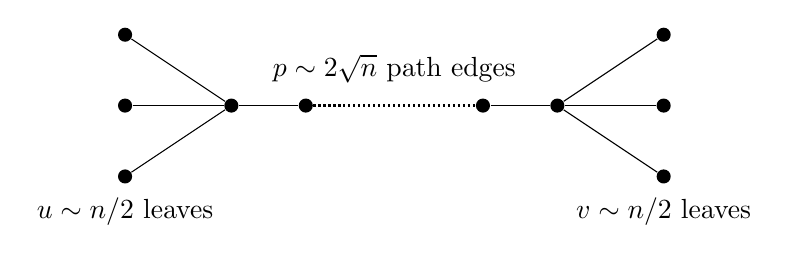
\begin{tikzpicture}[scale=.9,vertex/.style={circle,fill=black,inner sep=1.8pt}]
\node[vertex] (L) at (-2.3,0) {};
\node[vertex] (R) at (2.3,0) {};
\foreach \y in {-1,0,1} {
  \node[vertex] (a\y) at (-3.8,\y) {};
  \node[vertex] (b\y) at (3.8,\y) {};
  \draw (L)--(a\y); \draw (R)--(b\y);
}
\node[vertex] (A) at (-1.25,0) {};
\node[vertex] (B) at (1.25,0) {};
\draw (L)--(A); \draw[densely dotted,thick] (A)--(B); \draw (B)--(R);
\node at (0,.52) {$p\sim2\sqrt n$ path edges};
\node at (-3.8,-1.5) {$u\sim n/2$ leaves};
\node at (3.8,-1.5) {$v\sim n/2$ leaves};
\end{tikzpicture}
\caption{The balanced double-broom. Each fan denotes a larger family of
leaves. Leaf-edge cut counts are $n-1$, while central-path cut counts are
$n^2/4+O(n)$. Their proportions realize the extremal moment ratio.}
\label{p2:fig:double-broom}
\end{figure}

\subsection{A finite bound and its sharp asymptotic}

Define
\[
 M_n=\max\{\alpha(T):T\text{ is a tree on }n\text{ vertices}\},
 \quad
 a_n=\sqrt{n-1},
 \quad
 b_n=\sqrt{\lfloor n^2/4\rfloor}.
\]
The maximum exists because there are finitely many tree topologies on
$n$ vertices.

\begin{theorem}[Sharp tree approximation asymptotic]
\label{p2:thm:lewis-tree-sharp}
For every $n\geq2$ and every $n$-vertex tree $T$,
\begin{equation}\label{p2:eq:lewis-finite-upper}
 \alpha(T)\leq\frac{(a_n+b_n)^2}{4a_nb_n}.
\end{equation}
Moreover,
\begin{equation}\label{p2:eq:lewis-sharp-asymptotic}
 M_n=\frac{\sqrt n}{8}+\frac12+O(n^{-1/2})
 \qquad(n\longrightarrow\infty).
\end{equation}
Balanced double-brooms whose central paths have
$\lfloor2\sqrt n\rfloor$ edges attain the asymptotic in
\eqref{p2:eq:lewis-sharp-asymptotic}.
\end{theorem}

\begin{proof}
We first prove the upper bound.  Every tree edge satisfies
\[
 n-1\leq c_e\leq\lfloor n^2/4\rfloor.
\]
Put $x_e=\sqrt{c_e}$ and
$\mu=(n-1)^{-1}\sum_e x_e$.
The pointwise inequality $(x_e-a_n)(x_e-b_n)\leq0$ yields
\[
 \frac1{n-1}\sum_e x_e^2
 \leq(a_n+b_n)\mu-a_nb_n.
\]
By \eqref{p2:eq:lewis-tree-ratio},
\[
 \alpha(T)
 =\frac{(n-1)^{-1}\sum_e x_e^2}{\mu^2}
 \leq\frac{a_n+b_n}{\mu}-\frac{a_nb_n}{\mu^2}
 \leq\frac{(a_n+b_n)^2}{4a_nb_n}.
\]
For the last inequality one may maximize the scalar expression, whose
maximum occurs at $\mu=2a_nb_n/(a_n+b_n)$, or complete the square.
In particular,
\begin{equation}\label{p2:eq:lewis-upper-expansion}
 \frac{(a_n+b_n)^2}{4a_nb_n}
 =\frac{b_n}{4a_n}+\frac12+\frac{a_n}{4b_n}
 =\frac{\sqrt n}{8}+\frac12+O(n^{-1/2}).
\end{equation}

For the lower bound, fix $n\geq9$ and put
\[
 p=\lfloor2\sqrt n\rfloor,\qquad
 L=n-p-1,\qquad u=\lfloor L/2\rfloor,\qquad v=L-u.
\]
Take a path with $p$ edges, attach $u$ leaves to its left endpoint and
$v$ leaves to its right endpoint, and denote the resulting tree by
$T_n$.  It has exactly $n$ vertices and $n-1=L+p$ edges.
The $L$ leaf edges have cut count $n-1$.  For the $j$th path edge,
$1\leq j\leq p$, the cut count is
\begin{equation}\label{p2:eq:lewis-double-broom-cuts}
 c_j=(u+j)(n-u-j)=\frac{n^2}{4}-d_j^2,
 \qquad d_j=u+j-\frac n2.
\end{equation}
The choice of balanced leaf counts gives $|d_j|\leq p/2$.

Write $r=\sqrt n$ and $p=2r+t$, where $-1<t\leq0$.
Using $\sum_jd_j^2=O(p^3)$, we obtain
\begin{align}
 S_n:=\sum_{e\in E(T_n)}c_e
 &=L(n-1)+\frac{pn^2}{4}-\sum_{j=1}^{p}d_j^2\notag\\
 &=\frac{r^5}{2}+\left(\frac t4+1\right)r^4+O(r^3).
 \label{p2:eq:lewis-S-expansion}
\end{align}
For the square-root sum, the exact identity
\[
 0\leq\frac n2-\sqrt{\frac{n^2}{4}-d_j^2}
 =\frac{d_j^2}{n/2+\sqrt{n^2/4-d_j^2}}
 \leq\frac{2d_j^2}{n}
\]
shows that the total error on the path is $O(p^3/n)=O(r)$.
Since $\sqrt{n-1}=r-1/(2r)+O(r^{-3})$, it follows that
\begin{align}
 Q_n:=\sum_{e\in E(T_n)}\sqrt{c_e}
 &=L\sqrt{n-1}+\sum_{j=1}^{p}\sqrt{n^2/4-d_j^2}\notag\\
 &=2r^3+\left(\frac t2-2\right)r^2+O(r).
 \label{p2:eq:lewis-Q-expansion}
\end{align}
All remainder constants above are uniform in $t\in[-1,0]$ and in the
parity of $L$.
Substituting \eqref{p2:eq:lewis-S-expansion} and
\eqref{p2:eq:lewis-Q-expansion} into \eqref{p2:eq:lewis-tree-ratio} gives
\begin{align*}
 \alpha(T_n)
 &=\frac{(r^2-1)
       \{r^5/2+(t/4+1)r^4+O(r^3)\}}
       {4r^6+(2t-8)r^5+O(r^4)}\\
 &=\frac r8+\frac12+O(r^{-1}).
\end{align*}
The terms depending on $t$ cancel from the constant coefficient.
Together with \eqref{p2:eq:lewis-upper-expansion}, this proves
\eqref{p2:eq:lewis-sharp-asymptotic}.
\end{proof}

\begin{remark}[Why the extremal scale is a square root]
The ratio is the empirical second moment of the numbers
$\sqrt{c_e}$ divided by their squared empirical mean.
Leaf edges have $\sqrt{c_e}\simeq\sqrt n$, whereas the central edges of
a balanced double-broom have $\sqrt{c_e}\simeq n/2$.
About $2\sqrt n$ central edges balance these two contributions to the
first moment and asymptotically attain the interval moment bound.
Thus both the exponent and the leading constant arise from a genuine
extremal design calculation.
\end{remark}

\subsection{A rational certificate and the stated conjecture}

\begin{proposition}[An explicit finite counterexample]
\label{p2:prop:lewis-441}
Let $T$ consist of a path with $40$ edges, with $200$ new leaves
attached to each endpoint.  Then $T$ has $441$ vertices and
\[
 \alpha(T)>\frac{775676}{247107}>\frac{78}{25}=3.12.
\]
\end{proposition}

\begin{proof}
More generally, for an integer $k\geq1$, take a path with $4k$ edges
and attach $2k^2$ leaves to each endpoint.  Then $n=(2k+1)^2$ and
\[
 c_{\mathrm{leaf}}=n-1,
 \qquad
 c_j=(2k^2+j)(2k^2+4k+1-j),\quad 1\leq j\leq4k.
\]
Summation gives
\[
 S_k:=\sum_ec_e
 =\frac{4k}{3}(12k^4+36k^3+26k^2+6k+1).
\]
Since $\sqrt{n-1}<2k+1$ and $\sqrt{c_j}\leq n/2$,
\[
 Q_k:=\sum_e\sqrt{c_e}
 <4k^2(2k+1)+2kn
 =2k(2k+1)(4k+1).
\]
Therefore
\begin{equation}\label{p2:eq:lewis-rational-certificate}
 \alpha(T_k)>
 \frac{4(k+1)(12k^4+36k^3+26k^2+6k+1)}
      {3(2k+1)^2(4k+1)^2}.
\end{equation}
At $k=10$, the right-hand side is $775676/247107$, and
\[
 \frac{775676}{247107}-\frac{78}{25}
 =\frac{117554}{6177675}>0.
\]
Thus the certificate requires no floating-point approximation.
\end{proof}

\begin{corollary}[Negative resolution of the logarithmic comparison]
\label{p2:cor:lewis-conjecture-negative}
The $D$-optimal/infinity-Lewis effective-resistance approximation ratio
is not $O(\log n)$ on general graphs, or even on trees.
In particular, Conjecture~1.5 of
\cite{p2:SulimanWeinstein2023}, as stated in arXiv v1, is false.
The stronger Conjecture~4.6 in the same version is false as well.
\end{corollary}

\begin{proof}
Theorem~\ref{p2:thm:lewis-tree-sharp} supplies trees with
$\alpha(T_n)\sim\sqrt n/8$, and $\sqrt n/\log n\to\infty$.
The source's Theorem~1.4 bounds the actual approximation ratio above
by the quantity in its Conjecture~4.6, so that stronger proposed
logarithmic bound cannot hold either.
\end{proof}

\subsection{The subtree reduction does not preserve the ratio}

The discrepancy with the asserted constant tree bound can be traced
to a specific monotonicity step.  Claim~4.3 of
\cite{p2:SulimanWeinstein2023} asserts that $T\subset T'$ implies
$\alpha(T)\leq\alpha(T')$ for trees.  Under ordinary subtree
containment this assertion is false, as the following elementary
argument shows independently of the preceding asymptotic theorem.

\begin{proposition}[Failure of subtree monotonicity]
\label{p2:prop:lewis-nonmonotone}
There are trees $T\subset T'$ with $\alpha(T)>\alpha(T')$.
\end{proposition}

\begin{proof}
Take $T=P_4$, the path on four vertices.  Its cut counts are $3,4,3$;
hence
\[
 \alpha(P_4)=\frac{30}{(2\sqrt3+2)^2}>1.
\]
For $N\geq1$, attach $N$ new leaves to an endpoint of $P_4$, forming
$T_N\supset P_4$.  The new leaf edges have cut count $N+3$ and the
three original edges have cut counts
$3(N+1)$, $2(N+2)$, and $N+3$.  Thus
\[
 \sum_e c_e=N^2+9N+10,
\]
\[
 \sum_e\sqrt{c_e}
 =(N+1)\sqrt{N+3}+\sqrt{3(N+1)}+\sqrt{2(N+2)}
 =N^{3/2}+O(N^{1/2}).
\]
Since $|E(T_N)|=N+3$, formula \eqref{p2:eq:lewis-tree-ratio} gives
$\alpha(T_N)\to1$.  For all sufficiently large $N$,
$\alpha(T_N)<\alpha(P_4)$, proving the assertion.
\end{proof}

In the proposed monotonicity proof, a design on $T$ is treated as
feasible for the resistance problem on $T'$.  When vertices are
added, extending the old design by zero conductances disconnects
those new vertices and yields infinite total effective resistance;
it does not give the asserted comparison of optimal values.
The subsequent reduction from arbitrary bowties to a family with
three proportional size parameters therefore does not apply.
The extremal double-brooms above have a path of order $\sqrt n$ and
two leaf populations of order $n$, which is exactly the scale missed
by that reduction.


\section{Exact recurrence minimality for alternating binomial power sums}
\label{p2:sec:alternating}

For an integer $r\geq2$, consider McIntosh's alternating binomial sum
\begin{equation}\label{p2:eq:alt-definition}
 A_r(n)=\sum_{k=-n}^{n}(-1)^k\binom{2n}{n+k}^{r},\qquad n\geq0.
\end{equation}
McIntosh proved that this sequence has a polynomial-coefficient recurrence
with consecutive shift width at most $\lfloor r/2\rfloor$, and proved that
this width is minimal when $r$ is prime or a power of two
\cite[Theorems~1 and~2]{p3:McIntosh1993}. His lower-bound argument uses the
algebraic degree of the dominant exponential growth rate. That degree is
$\varphi(2r)/2$, which can be strictly smaller than $\lfloor r/2\rfloor$.
Here all the positive critical values of a real moment representation
provide the missing lower bounds.

By a recurrence we mean an eventual identity
\begin{equation}\label{p2:eq:alt-general-recurrence}
 \sum_{j\in J}q_j(n)A_r(n+j)=0,
 \qquad q_j\in\mathbb C(n)\setminus\{0\},
\end{equation}
where $J\subset\mathbb Z$ is finite and nonempty. Its \emph{shift width}
is $\max J-\min J$, and its \emph{number of terms} is $|J|$.
These are different quantities when the shifts have gaps.

\begin{theorem}\label{p2:thm:alt-minimality}
For every integer $r\geq2$, put $m=\lfloor r/2\rfloor$.
Every recurrence \eqref{p2:eq:alt-general-recurrence} has shift width at
least $m$ and at least $m+1$ nonzero terms. Both bounds are attained by
a recurrence with coefficients in $\mathbb Q[n]$.
Consequently the minimum shift width is $\lfloor r/2\rfloor$, and the
minimum number of terms, even allowing arbitrary gaps and coefficients
in $\mathbb C(n)$, is $\lfloor r/2\rfloor+1$.
\end{theorem}

The new assertion is the lower bound for every $r$, including the stronger
bound for sparse recurrences over $\mathbb C(n)$. Attainment uses the
general upper bound in McIntosh's Theorem~1. Thus the theorem removes the
prime-or-power-of-two restriction from his minimality conclusion; no
claim about an exhaustive historical priority search is needed for this
precise comparison.

\subsection{A positive moment representation}

Set $d=r-1$, $X=x_1\cdots x_d$, and
\begin{equation}\label{p2:eq:alt-laurent}
 P_r(x)=\prod_{i=1}^{d}(1+x_i)(1-X^{-1}).
\end{equation}
Here $\operatorname{CT}$ denotes the constant term in all $d$ variables.
For every integer $\ell\geq0$, direct expansion gives
\begin{equation}\label{p2:eq:alt-ct}
 \operatorname{CT}P_r^{\ell}
 =\sum_{j=0}^{\ell}(-1)^j\binom{\ell}{j}^{r}.
\end{equation}
Indeed, the term indexed by $j$ in the last factor forces the same
exponent $j$ in each of the other $d$ factors.

On $\mathbb T^d=(\mathbb R/2\pi\mathbb Z)^d$, write
$x_i=e^{i\theta_i}$ and $S=\sum_i\theta_i$. The elementary half-angle
identities yield
\begin{equation}\label{p2:eq:alt-real-function}
 P_r(e^{i\theta})=i\Psi_r(\theta),\qquad
 \Psi_r(\theta)=2^r\prod_{i=1}^{d}\cos(\theta_i/2)\sin(S/2).
\end{equation}
The half-angle expression is globally periodic: increasing one
$\theta_i$ by $2\pi$ changes both its cosine and the final sine by a
minus sign. Thus $\Psi_r=-iP_r|_{\mathbb T^d}$ is a globally real-analytic
real-valued function. Define
\begin{equation}\label{p2:eq:alt-positive-function}
 \Phi_r=\Psi_r^2=-P_r^2|_{\mathbb T^d}\geq0.
\end{equation}
For normalized Haar probability $\mu$ on the torus,
\begin{equation}\label{p2:eq:alt-positive-moment}
 A_r(n)=(-1)^n\operatorname{CT}P_r^{2n}
       =\int_{\mathbb T^d}\Phi_r(\theta)^n\,d\mu(\theta).
\end{equation}
The factor $(-1)^n$ comes from replacing $k$ by $j-n$ in
\eqref{p2:eq:alt-definition}. It is also exactly the factor contributed
by $P_r^{2n}=(-1)^n\Psi_r^{2n}$.

\subsection{The complete positive critical set}

\begin{lemma}\label{p2:lem:alt-critical-values}
The distinct positive critical values of $\Phi_r$ are
\begin{equation}\label{p2:eq:alt-values}
 v_j=\left(2\cos\frac{(2j+1)\pi}{2r}\right)^{2r},
 \qquad 0\leq j<m,\qquad m=\lfloor r/2\rfloor.
\end{equation}
Every critical point on each of these fibers is a nondegenerate local
maximum. There are no other critical points with $\Phi_r>0$.
\end{lemma}

\begin{proof}
At a point where $P_r\ne0$, all its factors are nonzero and
\begin{equation}\label{p2:eq:alt-critical-equations}
 x_i\frac{\partial}{\partial x_i}\log P_r
 =\frac{x_i}{1+x_i}+\frac1{X-1}.
\end{equation}
Its vanishing is equivalent to $x_iX=-1$. On the torus,
$\partial_{\theta_i}P_r=i x_i\partial_{x_i}P_r$; also $P_r=i\Psi_r$.
It follows that these equations are precisely the critical equations
for $\Psi_r$ away from its zero set. They force
$x_1=\cdots=x_d=\omega$ with $\omega^r=-1$. Conversely each such root
with $\omega\ne-1$ gives a critical point. The root $-1$ occurs only
for odd $r$ and has $P_r=0$, so it is excluded. Since
$d\Phi_r=2\Psi_r\,d\Psi_r$, this also exhausts the positive critical
set of $\Phi_r$.

At such a point $X=-1/\omega$, hence
$P_r=(1+\omega)^r$. With $\omega=e^{i(2j+1)\pi/r}$ this is
\[
 P_r=i(-1)^j
       \left(2\cos\frac{(2j+1)\pi}{2r}\right)^r.
\]
Conjugate roots produce equal values of $\Phi_r$. After pairing them,
the resulting values are exactly \eqref{p2:eq:alt-values}. Their angles
lie strictly between $0$ and $\pi/2$, so they are positive and strictly
decreasing. There are $m$ of them.

For the Hessian, let $I_d$ be the identity and $J_d$ the all-ones matrix.
Differentiating \eqref{p2:eq:alt-critical-equations} gives, at the critical
point,
\[
 \operatorname{Hess}_{\log x}\log P_r
 =\frac{\omega}{(1+\omega)^2}(I_d+J_d).
\]
The diagonal contribution is $\omega/(1+\omega)^2$. Every entry also
receives $-X/(X-1)^2$, which has the same value when $X=-1/\omega$.
If $\omega=e^{i\alpha}$, then
\[
 \frac{\omega}{(1+\omega)^2}
 =\frac1{4\cos^2(\alpha/2)}>0.
\]
Angular differentiation contributes a minus sign. On the real torus
one may use the real logarithm $\log|\Psi_r|$, whose Hessian agrees
with that of a local complex logarithm of $P_r$. Since the gradient
vanishes, this gives
\begin{equation}\label{p2:eq:alt-hessian}
 \operatorname{Hess}_{\theta}\Phi_r
 =-\frac{\Phi_r}{2\cos^2(\alpha/2)}(I_d+J_d).
\end{equation}
The eigenvalues of $I_d+J_d$ are $1$, with multiplicity $d-1$, and
$d+1=r$. The Hessian is therefore negative definite at every positive
critical point.
\end{proof}

\subsection{Visibility of every positive critical value}

We record the real-variable argument that prevents the smaller critical
values from disappearing under analytic continuation. In particular,
the argument includes the integer exponents that occur in even
dimensions.

\begin{lemma}\label{p2:lem:alt-visibility}
Let $M$ be a compact real-analytic manifold of dimension $d\geq1$, let
$\mu$ have a positive real-analytic density, and let $\Phi:M\to\mathbb R$
be real analytic. Suppose that the critical points in the fiber over
$v\ne0$ form a finite nonempty set and are all nondegenerate local
maxima. Regular points in that fiber are allowed. Then the generating
germ
\[
 F(t)=\int_M\frac{d\mu}{1-t\Phi}
\]
has a branch continued from $t=0$ that is singular at $t=1/v$.
\end{lemma}

\begin{proof}
The analytic Morse lemma gives local coordinates near each critical
point in which $\Phi=v-|y|^2$ and $d\mu=g(y)\,dy$, with $g$ analytic
and $g(0)>0$. For $w>0$ sufficiently small, the local density of
$\Phi_*\mu$ at $v-w$ is
\[
 \frac12w^{d/2-1}\int_{S^{d-1}}g(\sqrt w\,\omega)\,d\omega.
\]
The spherical average is analytic in $w$: odd Taylor terms integrate
to zero. Its constant term is positive. Choose smooth cutoffs equal
to one near the critical points. After restricting to a sufficiently
small interval about $v$, the remaining compact region contains only
regular points, so its pushforward has a smooth density. Summing the
critical contributions therefore gives
\begin{equation}\label{p2:eq:alt-density-defect}
 \frac{d\Phi_*\mu}{dx}(v+x)
 =b(x)+\mathbf 1_{\{x<0\}}(-x)^{d/2-1}h(-x),
\end{equation}
where $b$ is smooth, $h$ is analytic near zero, and $h(0)>0$.
There is no cancellation because all critical points contribute from
the same side with positive leading coefficients.

The density in \eqref{p2:eq:alt-density-defect} is not smooth at zero.
If $d$ is even, a finite derivative has a jump. If $d$ is odd and
$d\geq3$, a noninteger power prevents smoothness; for $d=1$, the
density is locally integrable but unbounded.

Consider the Cauchy transform
\[
 G(z)=\int_M\frac{d\mu}{z-\Phi}.
\]
It is holomorphic in the upper half-plane and satisfies
$G(z)=z^{-1}F(z^{-1})$ near infinity. Its boundary distribution is
\[
 -\frac1\pi\operatorname{Im}G(x+i0)=\Phi_*\mu,
\]
as follows from the Poisson kernel approximation to the identity.
If this upper-half-plane branch extended holomorphically through $v$,
its boundary imaginary part would be real analytic there. This
contradicts \eqref{p2:eq:alt-density-defect}. Thus the branch is singular
at $v$. The change of variables $t=1/z$, which is locally biholomorphic
at $v\ne0$, gives the claimed singularity at $1/v$. The continuation
from infinity in the upper half-plane corresponds to a continuation
of the generating germ from zero, including when $v$ is an interior
point of the real range of $\Phi$.
\end{proof}

Applying Lemmas~\ref{p2:lem:alt-critical-values} and
\ref{p2:lem:alt-visibility} to \eqref{p2:eq:alt-positive-moment} proves that
\begin{equation}\label{p2:eq:alt-generating-function}
 F_r(t)=\sum_{n\geq0}A_r(n)t^n
\end{equation}
has genuine continued-branch singularities at the $m$ distinct positive
points $t_j=1/v_j$. This assertion concerns all these continued
singularities, not merely the first singularity on the circle of
convergence.

\subsection{Singularities force width and support bounds}

\begin{lemma}\label{p2:lem:alt-sparse-budget}
Let $a_n$ have a generating function analytic near zero. Suppose its
continued germ has singularities at $m$ distinct positive finite
points. Then every eventual rational-coefficient recurrence for $a_n$
has shift width at least $m$ and at least $m+1$ nonzero terms, even if
its coefficients lie in $\mathbb C(n)$ and its shifts have gaps.
\end{lemma}

\begin{proof}
After translating the index, write the recurrence as
\[
 \sum_{j\in J}q_j(n)a_{n+j}=0,
 \qquad \min J=0,\qquad \max J=L.
\]
Clear denominators so that $q_j\in\mathbb C[n]$. Set
$e=\max_j\deg q_j$ and $c_j=[n^e]q_j$. Not all $c_j$ vanish.
Let $F(t)=\sum_{n\geq0}a_nt^n$ and $\vartheta=t\,d/dt$.
Multiplying by $t^{n+L}$ and summing over all sufficiently large $n$
gives
\begin{equation}\label{p2:eq:alt-recurrence-ode}
 \left(\sum_{j\in J}t^{L-j}q_j(\vartheta-j)\right)F(t)=R(t),
\end{equation}
where $R$ is a polynomial accounting for finitely many initial terms.
The coefficient of the highest ordinary derivative is $t^eH(t)$,
where
\begin{equation}\label{p2:eq:alt-leading-symbol}
 H(t)=\sum_{j\in J}c_jt^{L-j}\ne0.
\end{equation}
Distinct shifts give distinct monomials, so this leading coefficient
cannot vanish identically. Every nonzero finite singularity of a
continued solution of \eqref{p2:eq:alt-recurrence-ode} must be a zero of
$H$: otherwise the equation is an inhomogeneous linear differential
equation with an ordinary point and analytic right-hand side. For
$e=0$, the same conclusion follows directly from $H(t)F(t)=R(t)$.

Consequently $H$ has at least $m$ distinct positive roots. Since
$\deg H\leq L$, this implies $L\geq m$.
For the term bound, choose a nonzero real or imaginary part of $H$.
It is a real polynomial with the same $m$ positive roots and no more
nonzero monomials than $H$. Descartes' rule of signs implies that a
real polynomial with $k$ nonzero monomials has at most $k-1$ positive
roots. Thus $H$ has at least $m+1$ nonzero monomials. Formula
\eqref{p2:eq:alt-leading-symbol} now gives $|J|\geq m+1$.
\end{proof}

\begin{proof}[Proof of Theorem~\ref{p2:thm:alt-minimality}]
The moment representation and the complete critical-point calculation
give $m$ distinct positive singularities of $F_r$ by
Lemma~\ref{p2:lem:alt-visibility}. Lemma~\ref{p2:lem:alt-sparse-budget}
proves both lower bounds over $\mathbb C(n)$. McIntosh's general
existence theorem supplies a recurrence over $\mathbb Q[n]$ with shifts
in an interval of length $m$ \cite[Theorem~1]{p3:McIntosh1993}. It has at
most $m+1$ positions; the lower bounds force it to attain both claimed
minima.
\end{proof}

\begin{corollary}\label{p2:cor:alt-symbol}
For any minimum-width recurrence, translate the shifts to
$0,\ldots,m$ and define its highest-degree symbol $H$ by
\eqref{p2:eq:alt-leading-symbol}. Then
\begin{equation}\label{p2:eq:alt-exact-symbol}
 H(t)=c\prod_{j=0}^{m-1}(1-v_jt),\qquad c\ne0.
\end{equation}
The set of nonzero finite points at which some branch of $F_r$
continued from zero is singular is exactly $\{1/v_j:0\leq j<m\}$.
\end{corollary}

\begin{proof}
The polynomial $H$ has degree at most $m$ and already has the $m$
distinct roots $1/v_j$, so \eqref{p2:eq:alt-exact-symbol} follows.
The differential equation \eqref{p2:eq:alt-recurrence-ode} has no other
nonzero finite nonordinary points, hence no continued solution branch
can acquire a singularity elsewhere. Visibility supplies a singular
branch at every displayed point.
\end{proof}

\subsection{The first missing composite case}

For $r=6$, the three critical scales are
\[
 v_0=1351+780\sqrt3,\qquad v_1=64,\qquad
 v_2=1351-780\sqrt3.
\]
The dominant scale has algebraic degree two, so the dominant-growth
argument alone cannot prove the correct width three. The rational
interior scale $64$ supplies the third visible singularity. Theorem
\ref{p2:thm:alt-minimality} gives width three and at least four nonzero
terms for every sparse recurrence. Moreover,
\[
 \prod_{j=0}^{2}(X-v_j)
 =(X-64)(X^2-2702X+1)
 =X^3-2766X^2+172929X-64.
\]
Thus a minimum-width recurrence has highest-degree generating symbol
proportional to
\[
 1-2766t+172929t^2-64t^3.
\]
For comparison, $r=2$ and $r=3$ have the sole critical scales $4$ and
$27$, respectively, in agreement with the familiar hypergeometric
formulas $A_2(n)=\binom{2n}{n}$ and $A_3(n)=(3n)!/(n!)^3$.


% Section fragment. Uses amsmath, amssymb, amsthm and hyperref.
% Environments theorem, lemma, proposition, remark, proof are assumed.
\section{Nonresonant connection coefficients for Jacobi trace densities}
\label{p2:sec:jacobi-connection}

\subsection{The published connection problem and the new scope}

Forrester and Kumar explicitly identify the determination of the scalars
in the Frobenius representation of the Jacobi trace density as the
connection problem left by Davis.  Their Proposition 1.3 and equation
(3.55) solve that problem when the endpoint parameter $b$ and the Dyson
index $\beta$ are nonnegative integers.  Their discussion after equation
(3.54) states that the general problem remains; see
\emph{Differential recurrences for the distribution of the trace of the
$\beta$-Jacobi ensemble}, Physica D \textbf{434} (2022), 133220,
\texttt{arXiv:2011.00787v2}, Section 3.3 \cite{p8:SFB_FK}.

Here the corner Fourier amplitudes determine those physical-density
connection scalars for real, noninteger parameters, provided the local
exponents are nonintegral.  The answer uses an explicitly specified upper
half-plane continuation.  It generalizes the sign in the integer-parameter
formula to a complex phase.  The theorem concerns the particular physical
density, not the full connection matrix between arbitrary bases.  Resonant
exponents and numerical stability of long continuation chains are not
settled by it.

Fix
\begin{equation}\label{p2:eq:JC-parameters}
 N\ge1,\qquad a>-1,\qquad b>0,\qquad \beta\ge0.
\end{equation}
The stronger restriction $b>0$ makes every component of the published
auxiliary integral system absolutely integrable.  Define
\[
 S_N(a,b,\beta)=\int_{[0,1]^N}|\Delta(u)|^\beta
                    \prod_{i=1}^N u_i^a(1-u_i)^b\,du
\]
and let $\rho(t)$ be the density of $\sum_{i=1}^N u_i$ under this
normalized measure, extended by zero outside $[0,N]$.
For $r\ge0$ put
\begin{align*}
 W_r(q,\beta)
 &=\int_{(0,\infty)^r}e^{-\sum x_i}|\Delta(x)|^\beta
                                  \prod x_i^q\,dx,\qquad W_0=1,\\
 &=\prod_{j=0}^{r-1}
   \frac{\Gamma(q+1+j\beta/2)\Gamma(1+(j+1)\beta/2)}
        {\Gamma(1+\beta/2)}.
\end{align*}
Only $q=a,b>-1$ will occur.  The Laguerre--Selberg and Selberg
evaluations give this product and
\[
 S_N(a,b,\beta)=\prod_{j=0}^{N-1}
 \frac{\Gamma(a+1+j\beta/2)\Gamma(b+1+j\beta/2)
              \Gamma(1+(j+1)\beta/2)}
 {\Gamma(a+b+2+(N+j-1)\beta/2)\Gamma(1+\beta/2)}.
\]

For $0\le p\le N$ define
\begin{align}
 \alpha_p&=(N-p)(a+1)+\frac\beta2(N-p)(N-p-1),\notag\\
 \eta_p&=p(b+1)+\frac\beta2p(p-1),\notag\\
 D_p&=\alpha_p+\eta_p,\qquad \gamma_p=D_p-1,\label{p2:eq:JC-exponents}\\
 K_p&=\binom Np\frac{W_{N-p}(a,\beta)W_p(b,\beta)}{S_N(a,b,\beta)}.
 \label{p2:eq:JC-K}
\end{align}
Here $D_p>0$ and $K_p>0$.  Our nonresonance assumption is
\begin{equation}\label{p2:eq:JC-nonresonance}
 \gamma_p\notin\mathbb Z\qquad(0\le p<N).
\end{equation}
It removes a countable collection of parameter hyperplanes; it does not
require $a,b$ or $\beta$ to be rational.  The exponent at the final
endpoint $p=N$ need not be nonintegral, since no continuation across
that endpoint is needed to represent the density on $(0,N)$.

\subsection{The normalized Frobenius branches}

We specify the branches through the Forrester--Kumar system, so that the
normalization of the coefficients below is unambiguous.  With indices
$j=0,\ldots,N$, set
\[
 \Lambda=-\operatorname{diag}(N,N-1,\ldots,0),\qquad
 h=a+b+1+\tfrac\beta2(2N-1),\qquad k=b+\tfrac\beta2N,
\]
and let $X$ be tridiagonal, with entries
\begin{align*}
 X_{j,j-1}&=u_j=-jk+\tfrac\beta2j^2,\\
 X_{j,j}&=v_j=hj-\tfrac\beta2(N-j)(2j+1)+k(N-2j)-1,\\
 X_{j,j+1}&=w_j=h(j-N)+\tfrac\beta2(N-j)(N-j-1)+k(N-j).
\end{align*}
Entries outside the index range are omitted.  The published system is
\begin{equation}\label{p2:eq:JC-system}
 (tI+\Lambda)G'(t)=XG(t).
\end{equation}
To relate it to the physical density, form
\[
 H_j(t)=\binom Nj^{-1}\int_{[0,1]^N}
 \delta\Bigl(t-\sum u_i\Bigr)|\Delta(u)|^\beta
 \prod u_i^a(1-u_i)^{b-1}e_j(1-u_1,\ldots,1-u_N)\,du.
\]
If $P_{jk}=\binom{N-j}{N-k}$, then $G=P^{-1}H$ satisfies
\eqref{p2:eq:JC-system}.  The last row of $P$ is the last coordinate row,
so
\begin{equation}\label{p2:eq:JC-physical-component}
 G_N(t)=H_N(t)=S_N(a,b,\beta)\rho(t).
\end{equation}
These are Proposition 3.9 and equation (3.48) of the cited paper.
They also hold at $\beta=0$, by the same integration identities or
by continuity.  On every interval between the integers the system is
ordinary, so its distributional solution is real analytic there.

\begin{lemma}[A uniquely normalized singular branch]
\label{p2:lem:JC-Frobenius}
Fix $p\in\{0,\ldots,N\}$ with $\gamma_p\notin\mathbb Z$.
At $t=p$, the system \eqref{p2:eq:JC-system} has $N$ holomorphic local
solutions and one nonintegral Frobenius solution.  The last component
of the latter, after a unique constant normalization, has the form
\begin{equation}\label{p2:eq:JC-Fp}
 F_p(t)=(t-p)^{\gamma_p}U_p(t-p),\qquad U_p(0)=1,
\end{equation}
where $U_p$ is holomorphic with real Taylor coefficients.  Initially
$t-p>0$ and the power is positive real.  Any last component of a local
solution is the sum of a holomorphic function and a constant multiple
of this Frobenius branch, with the branch of the power specified.
\end{lemma}

\begin{proof}
Put $j_0=N-p$ and $s=t-p$.  The residue matrix is the matrix with
only row $j_0$ nonzero, that row being row $j_0$ of $X$.  It has
rank one, with its nonzero eigenvalue
\[
 v_{j_0}=\gamma_p-p=:v.
\]
This identity follows by substitution into the displayed definition
of $v_j$.  The hypothesis $\gamma_p\notin\mathbb Z$ implies that
$v$ is nonintegral, so the residue is diagonalizable with eigenvalues
$0$ and $v$, and no difference between them is a nonzero integer.
The ordinary nonresonant Frobenius construction gives $N$ holomorphic
solutions and one solution
\[
 s^v\sum_{\ell\ge0}g_\ell s^\ell,\qquad g_0=e_{j_0}.
\]
For completeness, substitution gives the recurrence
\[
 (v+\ell)(pI+\Lambda)g_\ell
       =(X-(v+\ell-1)I)g_{\ell-1}.
\]
Tridiagonality shows that its last component vanishes up to
$\ell=p-1$, while
\begin{equation}\label{p2:eq:JC-normalization}
 (g_p)_N=
 \frac{\prod_{\ell=1}^{p}u_{N-p+\ell}}
 {p!\prod_{\ell=1}^{p}(v+\ell)}\ne0.
\end{equation}
Indeed, the first contribution to row $N-p+\ell$ travels through
its subdiagonal entry $u_{N-p+\ell}$, and that row of
$pI+\Lambda$ has diagonal entry $\ell$.  Each numerator is
$-j(b+\beta(N-j)/2)$ with $j\ge1$, hence is nonzero by $b>0$;
the denominators are nonzero by nonresonance.  For $p=0$, the
empty product is one.  Division by \eqref{p2:eq:JC-normalization}
gives \eqref{p2:eq:JC-Fp}, since $v+p=\gamma_p$.  The nonintegral
Frobenius line is unique, and all coefficients are real.
\end{proof}

Write $F_p^{\uparrow}(t)$ for its continuation from just to the right
of $p$ to a real $t>p$, moving to the right and passing every intervening
integer by a small semicircle in the \emph{upper} half-plane.  This
fixes a homotopy class and hence a branch.  In particular, when a germ
on the left of a knot is continued to its right in this convention,
$(-s)^\gamma$ becomes $e^{-\pi i\gamma}s^\gamma$.

\subsection{The connection formula}

\begin{theorem}[Physical-density connection coefficients]
\label{p2:thm:JC-connection}
Assume \eqref{p2:eq:JC-parameters} and \eqref{p2:eq:JC-nonresonance}.
For $0\le p<N$ set
\begin{equation}\label{p2:eq:JC-Cp}
 \boxed{\displaystyle
 C_p=e^{-\pi i\eta_p}\frac{K_p}{\Gamma(D_p)}
 =e^{-\pi i\eta_p}\binom Np
 \frac{W_{N-p}(a,\beta)W_p(b,\beta)}
      {S_N(a,b,\beta)\Gamma(D_p)}.}
\end{equation}
For each $p\in\{0,\ldots,N-1\}$, let
$\rho_{p,-}^{\uparrow}$ be the continuation to the right of
$p$ of the density germ on its left, with the upper convention.
Let $\rho_{p,+}$ be its physical germ on the right.  At $p=0$
use the zero density on the exterior left interval.  Then
\begin{equation}\label{p2:eq:JC-local-jump}
 \rho_{p,+}(t)-\rho_{p,-}^{\uparrow}(t)=C_pF_p(t)
 \qquad(t>p\text{ sufficiently close to }p).
\end{equation}
Consequently, for $k=0,\ldots,N-1$ and $k<t<k+1$,
\begin{equation}\label{p2:eq:JC-global}
 \boxed{\displaystyle
 \rho(t)=\sum_{p=0}^{k}C_pF_p^{\uparrow}(t).}
\end{equation}
Although the summands can be complex, their sum is the real, positive
physical density.  The lower-half-plane formula is its complex conjugate.
If in addition $\gamma_N\notin\mathbb Z$, the local jump
\eqref{p2:eq:JC-local-jump} also holds at $p=N$, with the same formula
\eqref{p2:eq:JC-Cp} and zero physical density on the right.
\end{theorem}

The distinction between \eqref{p2:eq:JC-local-jump} and a one-sided real
coefficient is essential.  At noninteger parameters the density generally
has nonanalytic terms on \emph{both} sides of an interior knot.  The
coefficient $C_p$ is the discrepancy after a specified analytic
continuation; it is not, in general, the coefficient on the right alone.

\begin{lemma}[The complete local Fourier symbol]
\label{p2:lem:JC-symbol}
Fix $p\in\{0,\ldots,N\}$.  Let $\chi$ be smooth, supported in a
sufficiently small interval about $p$, and identically one near $p$.  Then as $R\to+\infty$,
\begin{equation}\label{p2:eq:JC-local-Fourier}
 \int e^{iRt}\chi(t)\rho(t)\,dt
 \sim e^{ipR}R^{-D_p}\sum_{\ell\ge0}A_{p,\ell}R^{-\ell},
 \qquad
 A_{p,0}=K_p e^{\frac{\pi i}{2}(\alpha_p-\eta_p)}.
\end{equation}
The expansion is complete to every prescribed finite order.
If $D_p$ is nonintegral, there are no additional integer-power terms
at this frequency.
\end{lemma}

\begin{proof}
Insert the defining pushforward integral for $\rho$.  The relevant
corners of the cube have $p$ coordinates equal to one and $N-p$
equal to zero.  Near one of these corners use $x_i=u_i$ in the
zero cluster and $y_i=1-u_i$ in the one cluster.  The phase becomes
$p+\sum x_i-\sum y_i$.  The weight is
\[
 |\Delta(x)|^\beta\prod x_i^a\;
 |\Delta(y)|^\beta\prod y_i^b\;B(x,y),
 \qquad B(0,0)=1,
\]
where $B$ is analytic near the origin.  The two homogeneous weights,
including their measures, have degrees $\alpha_p$ and $\eta_p$.
Radial integration with $r=\sum x_i$ and $q=\sum y_i$ reduces their
leading Fourier integrals to the one-dimensional endpoint formula
\[
 \int_0^\infty e^{\pm iRr}r^{d-1}\chi_0(r)\,dr
     \sim \Gamma(d)e^{\pm\pi i d/2}R^{-d},
 \quad d>0,
\]
where $\chi_0$ is smooth and equals one near zero.  For nonempty clusters the angular constants are
$W_{N-p}(a,\beta)/\Gamma(\alpha_p)$ and
$W_p(b,\beta)/\Gamma(\eta_p)$, respectively; an empty cluster
contributes one without radial integration.  The angular integrals
are over compact simplexes with integrable weights.  Consequently,
after choosing smooth cutoffs in $r$ and $q$, angular integration
of $B$ produces a smooth amplitude in these two radial variables,
with Taylor remainders of every order.  Applying the endpoint
formula successively in $r$ and $q$ gives a complete expansion.
Taylor expansion of $B$ gives only integer increments of $D_p$.
Thus one corner contributes the claimed leading coefficient without
the binomial factor, and all $\binom Np$ corners contribute identically.

To justify the complete expansion and exclude other contributions,
cover the complement of the corner neighbourhoods by small sets.
At every point of this complement, some cluster of coincident
coordinates lies strictly between zero and one.  Translating all
coordinates of that cluster together leaves its internal differences
unchanged, is tangent to all relevant collision faces, and has
nonzero phase derivative equal to the cluster size.  Other factors
in the translated coordinates are smooth and nonzero.  A smooth
partition of unity and repeated integration by parts in this
direction give an error $O(R^{-M})$ for every $M$, even when
$\beta$ is not integral.  Differentiated factors are bounded by
integrable endpoint and collision weights.  The radial endpoint
expansions of the corner pieces have remainders to arbitrary order.
This proves the complete expansion and the absence of another power
scale in \eqref{p2:eq:JC-local-Fourier}.
\end{proof}

\begin{proof}[Proof of Theorem~\ref{p2:thm:JC-connection}]
Fix a knot $p$ with $\gamma_p\notin\mathbb Z$, and abbreviate
$D=D_p$, $\gamma=\gamma_p$, $\alpha=\alpha_p$,
$\eta=\eta_p$, and $K=K_p$.  By
Lemma~\ref{p2:lem:JC-Frobenius}, on the two real sides of $s=t-p=0$
the physical density has the form
\begin{equation}\label{p2:eq:JC-two-sides}
 \rho(p+s)=
 \begin{cases}
  a_+(s)+c_+s^\gamma U_p(s),&s>0,\\
  a_-(s)+c_-(-s)^\gamma U_p(s),&s<0,
 \end{cases}
\end{equation}
where $a_\pm$ are holomorphic near zero and $c_\pm$ are real.
At an endpoint the exterior expression is zero.  The reality follows
from the real equation and the real normalization of $U_p$.

We first prove $a_+=a_-$.  After multiplication by a cutoff, a
nonzero first Taylor coefficient of $a_+-a_-$ of degree $q$ would
give a nonzero term of order $R^{-q-1}$ in the Fourier transform
at frequency $p$.  In contrast, the nonanalytic terms in
\eqref{p2:eq:JC-two-sides} give only powers $R^{-D-\ell}$,
$\ell\ge0$.  Since $D$ is nonintegral, the two power scales are
disjoint.  Lemma~\ref{p2:lem:JC-symbol} supplies a complete expansion
containing only the second scale.  Uniqueness of an asymptotic power
expansion forces every Taylor coefficient of $a_+-a_-$ to vanish.
The two holomorphic functions are therefore identical.  This step
is why leading asymptotics alone would not suffice for the proof.

Comparing the leading Fourier coefficient in
\eqref{p2:eq:JC-two-sides} with \eqref{p2:eq:JC-local-Fourier} gives
\[
 \Gamma(D)\left(c_+e^{\pi iD/2}+c_-e^{-\pi iD/2}\right)
       =K e^{\pi i(\alpha-\eta)/2}.
\]
The real and imaginary parts uniquely determine the two real
coefficients because $\sin(\pi D)\ne0$.  They are
\begin{equation}\label{p2:eq:JC-one-sided}
 c_+=\frac{K\sin(\pi\alpha)}{\Gamma(D)\sin(\pi D)},
 \qquad
 c_-=\frac{K\sin(\pi\eta)}{\Gamma(D)\sin(\pi D)}.
\end{equation}
These formulas remain meaningful when an individual sine in the
numerator vanishes.  They also cover the empty-cluster endpoints.

Under upper-half-plane continuation of the left germ,
$(-s)^\gamma$ becomes $e^{-\pi i\gamma}s^\gamma$.
As the analytic backgrounds agree, the discrepancy is
\[
 (c_+-e^{-\pi i\gamma}c_-)F_p(t).
\]
Using $D=\alpha+\eta$ and $\gamma=D-1$,
\[
 \sin(\pi\alpha)-e^{-\pi i\gamma}\sin(\pi\eta)
    =e^{-\pi i\eta}\sin(\pi D).
\]
Substitution into \eqref{p2:eq:JC-one-sided} gives exactly
$C_p=K e^{-\pi i\eta}/\Gamma(D)$ and proves
\eqref{p2:eq:JC-local-jump}.

At $p=0$ the density on the left is zero, so the first interval
satisfies $\rho=C_0F_0$.  Continue this identity to the next knot
through the specified upper path and add the local discrepancy
$C_1F_1$.  The identity extends throughout the next interval by
analytic continuation of the same differential system.  Inductively,
this proves \eqref{p2:eq:JC-global}.  Reversing upper and lower paths
conjugates the coefficients and branches.
\end{proof}

\subsection{Comparison, checks, and limitations}

When $b$ is a positive integer and $\beta$ is a nonnegative integer,
\[
 \eta_p=p(b+1)+\frac\beta2p(p-1)\in\mathbb Z,
 \qquad e^{-\pi i\eta_p}=(-1)^{p(b+1)+\beta p(p-1)/2}.
\]
If $a$ is irrational, all exponents $\gamma_p$ with $p<N$ are
nonintegral.  Thus the theorem has a nonempty intersection with the
integer-parameter result, and \eqref{p2:eq:JC-Cp} there is exactly the
sign and Laguerre--Selberg constant of Forrester--Kumar (1.12),
Proposition 3.4, and (3.55).  Their $b=0$ boundary case is not included
in the present auxiliary-integral hypothesis.
The new range is the nonresonant real-parameter range outside those
integer restrictions.  In that range the coefficient on the left of
an interior knot generally does not vanish, and the continuation
convention is indispensable.

As an exact consistency test of the additional final-endpoint
statement, take $N=1$ and $a,b\notin\mathbb Z$.  The density is
$t^a(1-t)^b/B(a+1,b+1)$ on $(0,1)$.  At $t=1$ its upper
continuation is $e^{-\pi ib}(t-1)^b t^a/B(a+1,b+1)$.
Formula \eqref{p2:eq:JC-Cp} gives
$C_1=e^{-\pi i(b+1)}/B(a+1,b+1)$, precisely the coefficient
that cancels this branch to produce the zero exterior density.

A second, noninteger numerical diagnostic uses the exact $N=2$
hypergeometric density in Forrester--Kumar (3.36)--(3.37).
For $a=0.2$, $b=0.35$, $\beta=0.7$, the predicted coefficient at
$p=1$ is
\[
 C_1=-3.7279987849354161471+7.3166095798246842339\,i.
\]
Evaluating the difference between the physical right density and the
upper continuation of the left density, then dividing by
$(t-1)^{a+b+1}$, converges to this value as $t\downarrow1$.
This diagnostic does not replace the proof.

\begin{remark}[Remaining questions]
This result does not assert a full connection matrix for arbitrary
Frobenius bases, a uniform error bound for numerical continuation,
or a treatment of resonant $\gamma_p\in\mathbb Z$.  Resonance can
introduce logarithms and requires a separately normalized limiting
basis; simply substituting resonant parameters into
\eqref{p2:eq:JC-one-sided} would be invalid.  The condition $b>0$
has also been retained instead of asserting an unproved extension
through divergent auxiliary integrals.  A broader priority audit
of general Selberg connection formulas remains necessary before
any claim of historical first solution.
\end{remark}


% Section fragment.  Required packages: amsmath, amssymb, amsthm, hyperref.
% Bibliography entry for the parent document:
% \bibitem{abraham2025frontiers} K. Abraham, E. Gassiat and Z. Naulet,
% Frontiers to the learning of nonparametric hidden Markov models,
% Journal of Machine Learning Research 26(155) (2025), 1--75.
% https://jmlr.org/papers/v26/24-2230.html

\section{One hidden-refresh trajectory: sharp costs at both persistence boundaries}
\label{p2:sec:long-chain}

A population that is invisible from one observation can become identifiable
through temporal dependence.  For a fixed known emission family, the preceding
three-visit construction gives a persistence-dependent rate from independent
triples.  This section removes that independence assumption: all observations
now come from one stationary trajectory.  Two distinct obstructions must be
controlled simultaneously.  As persistence tends to zero, the one-view defect
reappears.  As persistence tends to one, the trajectory contains too few fresh
population draws.  We obtain matching upper and lower bounds over an interval
containing both boundaries, using an estimator that knows neither boundary
margin.  The proof of the small-persistence lower bound compares full-history
filters; a calculation for isolated triples alone would not suffice.

\subsection{A fixed analytic emission family and the statistical experiment}

Let $U$ be uniform probability on $[0,1]$, and write
$L_j(x)=P_j(2x-1)$ for the shifted Legendre polynomial of degree $j$.
Set
\begin{equation}\label{p2:eq:lc-kernel}
 v_j(\theta)=\theta^j-\frac{2\theta}{j+1},\qquad
 k(x\mid\theta)=1+\sum_{j=2}^{\infty}
                  \frac{L_j(x)v_j(\theta)}{8j!},
 \quad x,\theta\in[0,1].
\end{equation}
The family $k$ is known.  Factorial decay makes the series normally convergent
on every compact subset of $\mathbb C^2$, so it defines an entire function.
The identities $\int L_j\,dU=0$ and $\int v_j\,dU=0$ show that
\begin{equation}\label{p2:eq:lc-cancellation}
 \int k(x\mid\theta)\,dU(x)=1,
 \qquad k(x\mid0)=1,
 \qquad \int k(x\mid\theta)\,dU(\theta)=1.
\end{equation}
Since $|L_j|\le1$ and $|v_j|\le2$ on the real unit interval,
\begin{equation}\label{p2:eq:lc-bounds}
 |k-1|\le\frac{e-2}{4}<\frac14,
 \qquad \frac34\le k\le\frac54.
\end{equation}
In particular $k(\cdot\mid\theta)$ is a strictly positive probability density.

For $s\in[1/2,1]$ let
\begin{equation}\label{p2:eq:lc-population}
 G_s=(1-s)\delta_0+sU.
\end{equation}
The latent chain is stationary with population $G_s$ and transition kernel
\begin{equation}\label{p2:eq:lc-transition}
 M_{s,\rho}(\theta,d\eta)
   =\rho\delta_\theta(d\eta)+(1-\rho)G_s(d\eta),
 \qquad 0<\rho<1.
\end{equation}
Conditionally on the latent path, observations are independent with density
$k(\cdot\mid\theta_i)$.  Both $s$ and $\rho$ are unknown.  The data consist of
\emph{one complete trajectory} $(X_1,\ldots,X_n)$; denote its law by
$\mathsf P^{(n)}_{s,\rho}$.  By \eqref{p2:eq:lc-cancellation}, every individual
observation has law $U$, independently of $s$ and $\rho$.

We estimate the population in Wasserstein distance $W_1$ for the usual metric
on $[0,1]$.  The one-dimensional distribution-function formula gives
\begin{equation}\label{p2:eq:lc-wasserstein}
 W_1(G_s,G_t)=\frac{|s-t|}{2}.
\end{equation}
The infima below allow arbitrary measurable probability-valued estimators,
not just estimates within the family \eqref{p2:eq:lc-population}.

\begin{theorem}[Two-boundary minimax rate from one path]
\label{p2:thm:lc-main}
For $0<r\le1/8$, $0<q\le1/4$ and $n\ge1$, define
\[
 R_n(r,q)=\inf_{\widehat G}\ 
 \sup_{\substack{s\in[1/2,1]\\\rho\in[r,1-q]}}
 \mathbb E_{s,\rho}W_1(\widehat G,G_s).
\]
There are constants $0<c<C<\infty$, depending only on the fixed emission
family, such that
\begin{equation}\label{p2:eq:lc-main-rate}
 c\min\left\{1,\frac{r^{-2}+q^{-1/2}}{\sqrt n}\right\}
 \le R_n(r,q)\le
 C\min\left\{1,\frac{r^{-2}+q^{-1/2}}{\sqrt n}\right\}.
\end{equation}
A single estimator $\widehat G_n$, using neither $r$ nor $q$, satisfies the
stronger pointwise upper bound
\begin{equation}\label{p2:eq:lc-pointwise}
 \mathbb E_{s,\rho}W_1(\widehat G_n,G_s)
 \le C\min\left\{1,\frac1{\sqrt n\,\rho^2\sqrt{1-\rho}}\right\},
 \qquad s\in[1/2,1],\quad 0<\rho<1.
\end{equation}
\end{theorem}

The rate in \eqref{p2:eq:lc-main-rate} contains the sum, equivalently the maximum,
of two boundary costs.  A product $r^{-2}q^{-1/2}$ would lose this information:
one value of $\rho$ cannot lie close to both zero and one.  The restrictions on
$r,q$ guarantee that both lower-bound experiments lie in the parameter
interval; the upper bound applies throughout that interval, including its
interior.

\begin{corollary}[Exact uniform-consistency criterion]
\label{p2:cor:lc-consistency}
For sequences $r_n\in(0,1/8]$ and $q_n\in(0,1/4]$, uniform consistent
population estimation over the corresponding classes is possible if and only if
\[
 nr_n^4\longrightarrow\infty
 \qquad\hbox{and}\qquad nq_n\longrightarrow\infty.
\]
\end{corollary}
\begin{proof}
Apply both sides of \eqref{p2:eq:lc-main-rate}.  A sum of two nonnegative
sequences tends to zero exactly when both summands do.
\end{proof}

\subsection{An estimator that needs neither persistence margin}

Let $\phi=80L_2$ and $a=2/135$.  Legendre orthogonality gives
\[
 \int \phi(x)k(x\mid\theta)\,dU(x)=v_2(\theta),
 \qquad \int v_2(\theta)^2\,dU(\theta)
 =\frac15-\frac13+\frac4{27}=a.
\]
Also $v_2(0)=0$ and $\int v_2\,dU=0$.  The refresh transition has powers
$M_{s,\rho}^h=\rho^h I+(1-\rho^h)G_s$.  Conditional independence of
emissions therefore yields, for every integer $h\ge1$,
\begin{equation}\label{p2:eq:lc-moments}
 \mathbb E_{s,\rho}
    \frac{\phi(X_i)\phi(X_{i+h})}{a}=s\rho^h.
\end{equation}

For $n\ge4$, put $m=n-2$ and define the overlapping-window averages
\[
 \widehat V=\frac1m\sum_{i=1}^{m}
                  \frac{\phi(X_i)\phi(X_{i+1})}{a},\qquad
 \widehat W=\frac1m\sum_{i=1}^{m}
                  \frac{\phi(X_i)\phi(X_{i+2})}{a}.
\]
Their mean vector is $(v,w)=(s\rho,s\rho^2)$.

\begin{lemma}[Variance of overlapping windows]\label{p2:lem:lc-variance}
There is a fixed constant $C$ such that
\begin{equation}\label{p2:eq:lc-variance}
 \mathbb E_{s,\rho}
       \bigl[(\widehat V-v)^2+(\widehat W-w)^2\bigr]
 \le\frac C{n(1-\rho)}.
\end{equation}
\end{lemma}
\begin{proof}
Each summand is a bounded function of the block $(X_i,X_{i+1},X_{i+2})$.
For two such blocks with starting positions separated by $\ell\ge3$,
condition on the latent state at the right endpoint of the first block and
the state at the left endpoint of the second.  Across the intervening gap,
the transition is
\[
 M_{s,\rho}^{\ell-2}
   =\rho^{\ell-2}I+(1-\rho^{\ell-2})G_s.
\]
The second term produces the product of the two expectations.  It follows
that the absolute covariance is at most $C\rho^{\ell-2}$.  Overlaps with
$\ell\le2$ have covariance at most $C$.  Summing the covariance series,
and using $m\ge n/2$, proves \eqref{p2:eq:lc-variance}.
\end{proof}

Choose a measurable minimizer $(\widehat s,\widehat\rho)$ of
\begin{equation}\label{p2:eq:lc-projection}
 (\widehat V-s'\rho')^2+(\widehat W-s'\rho'^2)^2
 \quad\hbox{over}\quad
 (s',\rho')\in[1/2,1]\times[0,1].
\end{equation}
Existence follows from compactness and continuity; a fixed measurable
tie-breaking rule supplies measurability.  Set $\widehat G_n=G_{\widehat s}$.
For $n<4$, use a fixed member of the population family.

\begin{lemma}[A global inverse with the true persistence in its denominator]
\label{p2:lem:lc-inverse}
Let $s,s'\in[1/2,1]$, $0<\rho\le1$, $0\le\rho'\le1$, and put
$(v,w)=(s\rho,s\rho^2)$ and $(v',w')=(s'\rho',s'\rho'^2)$.  Then
\begin{equation}\label{p2:eq:lc-inverse}
 |s-s'|\le\frac4{\rho^2}
                 \bigl(|v-v'|+|w-w'|\bigr).
\end{equation}
The candidate persistence $\rho'$ may be zero.
\end{lemma}
\begin{proof}
The polynomial identities $v^2=sw$ and $v'^2=s'w'$ hold even at $\rho'=0$.
Consequently
\[
 w(s-s')=v^2-v'^2+s'(w'-w).
\]
Since $w\ge\rho^2/2$, $v,v'\in[0,1]$ and $s'\le1$, the claimed bound follows.
\end{proof}

\begin{proof}[Proof of the upper bounds in Theorem~\ref{p2:thm:lc-main}]
Least-squares projection makes the Euclidean error of the fitted moment
vector at most twice the empirical error from the true moment vector.
Lemma~\ref{p2:lem:lc-inverse}, Cauchy--Schwarz and
Lemma~\ref{p2:lem:lc-variance} give
\[
 \mathbb E_{s,\rho}|\widehat s-s|
     \le\frac C{\sqrt n\,\rho^2\sqrt{1-\rho}}.
\]
The error is also bounded by $1/2$.  Equation~\eqref{p2:eq:lc-wasserstein}
proves \eqref{p2:eq:lc-pointwise}, after increasing the constant to include
$n<4$.  Crucially, the persistence in this bound is the true parameter,
not a worst-case lower bound substituted before the variance calculation.

For $\rho\le1/2$, the right-hand side before clipping is at most
$C/(\sqrt n\,r^2)$.  For $\rho\ge1/2$, it is at most
$C/\sqrt{nq}$.  Taking the supremum over $[r,1-q]$, then using the bounded
loss, proves the upper half of \eqref{p2:eq:lc-main-rate}.
\end{proof}

\subsection{Small persistence: a full-path information bound}

The moment map has first coordinate $s\rho$.  We compare two parameter
points along a curve on which this coordinate is constant.  The next lemma
shows that the entire observed trajectory, including all its long-range
dependence, has only fourth-order information in small persistence along
that curve.  Write $D(P\Vert Q)$ for relative entropy.

\begin{lemma}[Uniform filter comparison along $s\rho=\textnormal{constant}$]
\label{p2:lem:lc-filter}
Suppose $s,s'\in[1/2,1]$, $0<\rho,\rho'\le1/4$ and
$\alpha=s\rho=s'\rho'$.  Then, for every $n\ge1$,
\begin{equation}\label{p2:eq:lc-path-kl}
 D\bigl(\mathsf P^{(n)}_{s,\rho}
             \Vert\mathsf P^{(n)}_{s',\rho'}\bigr)
       \le Cn\alpha^2(\rho-\rho')^2.
\end{equation}
The constant is independent of the time horizon and both parameters.
\end{lemma}
\begin{proof}
Put $q_x(\theta)=k(x\mid\theta)-1$.  For a fixed observed history
$(x_1,\ldots,x_t)$, let $f_t^{s,\rho}$ be the posterior density of
$\theta_t$ relative to $G_s$.  Use the recursive formula below to extend
this density to a function on all of $[0,1]$.  With $f_0=1$, Bayes' formula
gives
\begin{align}
 f_t^{s,\rho}(\theta)
   &=\frac{k(x_t\mid\theta)
                    [1-\rho+\rho f_{t-1}^{s,\rho}(\theta)]}
           {p_t^{s,\rho}(x_t)},\label{p2:eq:lc-filter-recursion}\\
 p_t^{s,\rho}(x)
   &=1+s\rho\int q_x(\theta)
                         f_{t-1}^{s,\rho}(\theta)\,dU(\theta).
                         \label{p2:eq:lc-predictive}
\end{align}
Here $p_t^{s,\rho}$ is the conditional density of $X_t$ given the preceding
history.  To check the second formula, integrate the numerator of the first
before observing $x_t$.  The constant part integrates to one because
$\int f_{t-1}^{s,\rho}\,dG_s=1$; the remaining part uses
$\int q_x\,dG_s=0$ and $q_x(0)=0$.  For $t=1$, the convention $f_0=1$
gives the stationary initial law and $p_1=1$.

Every predictive distribution is a mixture of emission densities, so
\begin{equation}\label{p2:eq:lc-predictive-bounds}
 \frac34\le p_t^{s,\rho}\le\frac54
\end{equation}
for every history, including histories of probability zero.  Indeed all
formulas are pointwise defined with positive denominators.
An induction in \eqref{p2:eq:lc-filter-recursion} gives
\begin{equation}\label{p2:eq:lc-filter-bound}
 \|f_t^{s,\rho}\|_\infty\le3.
\end{equation}
If the preceding norm is at most three, the next one is at most
$(5/3)(1-\rho+3\rho)\le5/2<3$; the induction starts at $f_0=1$.

Compare both filters on the same arbitrary history, and write
$\Delta_t=\|f_t^{s,\rho}-f_t^{s',\rho'}\|_\infty$.
Equation~\eqref{p2:eq:lc-predictive}, the fixed value of $\alpha$, and
$\|q_x\|_\infty\le1/4$ imply
\begin{equation}\label{p2:eq:lc-predictive-difference}
 \sup_x|p_t^{s,\rho}(x)-p_t^{s',\rho'}(x)|
       \le\frac\alpha4\Delta_{t-1}.
\end{equation}
If $N,N'$ denote the numerators in
\eqref{p2:eq:lc-filter-recursion}, then
\[
 \|N-N'\|_\infty
 \le\frac54\bigl(\rho\Delta_{t-1}+4|\rho-\rho'|\bigr).
\]
This follows by adding and subtracting $\rho f_{t-1}^{s',\rho'}$
and using \eqref{p2:eq:lc-filter-bound}.
Using $N'/p'=f_t^{s',\rho'}$, whose norm is at most three, and
\eqref{p2:eq:lc-predictive-bounds}, we obtain
\[
 \Delta_t
 \le\left(\frac53\rho+\alpha\right)\Delta_{t-1}
                         +\frac{20}{3}|\rho-\rho'|
 \le\frac23\Delta_{t-1}+\frac{20}{3}|\rho-\rho'|.
\]
The last inequality uses $\alpha\le\rho\le1/4$.
Since $\Delta_0=0$, geometric summation proves
$\Delta_t\le20|\rho-\rho'|$ uniformly in time and history.  Therefore
\begin{equation}\label{p2:eq:lc-uniform-predictive-difference}
 \sup_x|p_t^{s,\rho}(x)-p_t^{s',\rho'}(x)|
       \le5\alpha|\rho-\rho'|.
\end{equation}

For two densities $p,p'$ relative to the probability measure $U$,
$D(p\Vert p')\le\int(p-p')^2/p'\,dU$.  Equations
\eqref{p2:eq:lc-predictive-bounds} and
\eqref{p2:eq:lc-uniform-predictive-difference} thus bound every conditional
relative entropy by $C\alpha^2(\rho-\rho')^2$, uniformly in the preceding
history.  Summing by the chain rule for relative entropy gives
\eqref{p2:eq:lc-path-kl}.
\end{proof}

\begin{proposition}[The small-persistence obstruction]
\label{p2:prop:lc-small-persistence}
On the parameter class of Theorem~\ref{p2:thm:lc-main},
\begin{equation}\label{p2:eq:lc-small-lower}
 R_n(r,q)\ge c\min\{1,(\sqrt n\,r^2)^{-1}\}.
\end{equation}
\end{proposition}
\begin{proof}
Take
\[
 s_0=\frac34,\quad \rho_0=\frac{3r}{2},\qquad
 s_1=s_0+h,\quad \rho_1=\rho_0\frac{s_0}{s_1},
 \qquad 0<h\le\frac18.
\]
Both persistence values belong to $[r,1-q]$ and are at most $1/4$.
Their products $s_i\rho_i$ agree, and
$|\rho_0-\rho_1|\le Crh$.  Lemma~\ref{p2:lem:lc-filter} gives
\[
 D\bigl(\mathsf P^{(n)}_{s_0,\rho_0}
             \Vert\mathsf P^{(n)}_{s_1,\rho_1}\bigr)
     \le Cnh^2r^4.
\]
Choose $h=c_0\min\{1,(\sqrt n\,r^2)^{-1}\}$ with a fixed sufficiently
small $c_0>0$.  Then the total variation distance of the two observed-path
laws is at most $1/2$, by Pinsker's inequality.  Their population separation
is $h/2$ by \eqref{p2:eq:lc-wasserstein}.  For any probability-valued estimator,
the nearest-population test and the triangle inequality give a maximal
expected loss at least one quarter of this separation times one minus the
total variation distance.  This proves \eqref{p2:eq:lc-small-lower}.
\end{proof}

\subsection{Nearly frozen paths: only fresh latent draws carry population information}

\begin{proposition}[The nearly frozen obstruction]
\label{p2:prop:lc-frozen}
On the parameter class of Theorem~\ref{p2:thm:lc-main},
\begin{equation}\label{p2:eq:lc-frozen-lower}
 R_n(r,q)\ge\frac c{\sqrt{1+nq}}
             \ge c'\min\{1,(nq)^{-1/2}\}.
\end{equation}
\end{proposition}
\begin{proof}
Fix $\rho=1-q$.  Consider an oracle that reveals all refresh indicators,
the initial latent value, and every newly drawn latent value.  The oracle
can simulate the whole observed path using a parameter-independent Markov
kernel, so data processing bounds observed-path relative entropy by oracle
relative entropy.  The number of independent population draws revealed is
\[
 M=1+\operatorname{Binomial}(n-1,q),
 \qquad \mathbb E M=1+(n-1)q.
\]
Refresh indicators have the same law at all values of $s$.  Because $\delta_0$
and $U$ are mutually singular,
\[
 D(G_s\Vert G_t)
   =s\log\frac{s}{t}+(1-s)\log\frac{1-s}{1-t}.
\]
For $s_0=3/4$ and $s_1=s_0+h$, $0<h\le1/8$, this is at most $Ch^2$.
Conditioning on the indicators and averaging the product-law relative
entropies therefore gives
\[
 D\bigl(\mathsf P^{(n)}_{s_0,1-q}
             \Vert\mathsf P^{(n)}_{s_1,1-q}\bigr)
       \le C(1+nq)h^2.
\]
Choose $h=c_0/\sqrt{1+nq}$ and apply the same two-point argument as before.
The resulting bound is $c/\sqrt{1+nq}$.  This is comparable, with absolute
constants, to $\min\{1,(nq)^{-1/2}\}$.
\end{proof}

\begin{proof}[Completion of Theorem~\ref{p2:thm:lc-main}]
The upper bound has already been proved.  The maximum of the lower bounds
in Propositions~\ref{p2:prop:lc-small-persistence} and~\ref{p2:prop:lc-frozen}
is, within an absolute constant, their clipped sum.  Explicitly, for
$A,B\ge0$,
\[
 \max\{\min(1,A),\min(1,B)\}
       \ge\tfrac12\min(1,A+B).
\]
Taking $A=(\sqrt n\,r^2)^{-1}$ and $B=(nq)^{-1/2}$ proves the lower
half of \eqref{p2:eq:lc-main-rate}.
\end{proof}

\begin{remark}[The two endpoints are different impossibility mechanisms]
At $\rho=0$, all observed paths are independent uniform samples for every
$s$, so the population is unidentifiable.  At $\rho=1$, the oracle above
reveals just one population draw, regardless of the length of the observed
path.  The same two-point argument then gives a positive constant minimax
risk for every $n$.  Thus the obstruction at one is lack of fresh population
draws, even though the emission law of the retained latent state may be
learned accurately from its long run.
\end{remark}

\subsection{Transfer conditions and precise relation to earlier work}

\begin{proposition}[The same rate for other fixed emission families]
\label{p2:prop:lc-general-kernel}
Let $\Theta$ be a compact metric space, let $\theta_0\in\Theta$, and let
$H$ be a probability measure with $H(\{\theta_0\})=0$.  Let $\mu$ be a
probability measure on the observation space.  Suppose the known emission
densities satisfy, pointwise,
\begin{gather*}
 |k(x\mid\theta)-1|\le\frac14,\qquad
 k(x\mid\theta_0)=1,\qquad
 \int k(x\mid\theta)\,dH(\theta)=1,\\
 \int k(x\mid\theta)\,d\mu(x)=1.
\end{gather*}
Assume there is a bounded measurable real function $\phi$ with
$\int\phi\,d\mu=0$ such that
\[
 b(\theta)=\int\phi(x)k(x\mid\theta)\,d\mu(x),\qquad
 a=\int b(\theta)^2\,dH(\theta)>0.
\]
Replace $U$ by $H$ and $0$ by $\theta_0$ in the population
\eqref{p2:eq:lc-population}, and use the same refresh transition.  Then
Theorem~\ref{p2:thm:lc-main} and Corollary~\ref{p2:cor:lc-consistency} hold, with
constants depending on this fixed experiment and its metric.
\end{proposition}
\begin{proof}
The assumptions give $b(\theta_0)=0$ and $\int b\,dH=0$.  For $h=1,2$,
the bounded statistic $\phi(X_i)\phi(X_{i+h})/a$ again has expectation
$s\rho^h$.  The covariance bound and moment inverse are
unchanged.  Also
\[
 W_1(G_s,G_t)
    =|s-t|\int d(\theta_0,\theta)\,dH(\theta).
\]
The upper bound follows by coupling the excess mass between $\delta_{\theta_0}$
and $H$, and the reverse inequality follows from the 1-Lipschitz function
$d(\theta_0,\cdot)$.  The displayed multiplier is strictly positive.

For the small-persistence lower bound, the filter proof is identical with
$H$ replacing $U$ in latent integrals and $\mu$ replacing $U$ in predictive
relative entropies.  Every numerical bound in that proof used only the stated
bound $|k-1|\le1/4$ and the two cancellation identities.  Finally,
$H(\{\theta_0\})=0$ gives the same Bernoulli relative entropy for population
draws, proving the nearly frozen lower bound.  This verifies all assertions.
\end{proof}

The direct advance over the independent-three-visit result is the matching
rate for a single dependent path, including both persistence boundaries and
an estimator that does not require their margins.  The small-persistence
lower bound required a separate full-path argument; it cannot be obtained
by declaring overlapping triples independent or by substituting an informal
effective sample size.

For comparison, Abraham, Gassiat and Naulet study minimax frontiers for
nonparametric hidden Markov models with unknown emission
densities~\cite{p2:abraham2025frontiers}.  Their Section~1.2 distinguishes the
independence boundary from an absolute spectral-gap condition, and their
informal Theorem~1 allows constants to depend on that gap.  Section~4 states
that exact dependence on the gap was not its focus, and poses a different
adaptation question concerning emission densities of different smoothness.
The present theorem does not resolve that question: the emission family is
fixed and known, the population submodel is one-dimensional, and transitions
have the restricted refresh form \eqref{p2:eq:lc-transition}.  Within this
specified experiment, both boundary dependences in
\eqref{p2:eq:lc-main-rate} are proved sharply.

Although the population has only one scalar unknown coefficient, the latent
state is continuous.  A value drawn from the continuous part retains its own
emission law throughout a persistence run.  Collapsing all such values into
one of two state labels and assigning that label a fixed emission law would
remove the within-run dependence and would change the experiment.


\section{What has and has not been resolved}

The double-broom construction is an explicit obstruction to the logarithmic
Lewis-weight claim under the source's own normalization. The result
determines the worst tree asymptotic, including its leading coefficient
and constant term. It does not determine the worst asymptotic over all
connected graphs.

For alternating binomial sums, the lower bound holds for every integer
exponent and for coefficients in $\mathbb C(n)$, with no coefficient-degree
restriction. The matching upper bound is credited to McIntosh. We remove
the restriction in his theorem; we do not assert that an exhaustive survey
has certified the absence of every subsequent proof.

For Jacobi traces, the conclusion gives the scalars for the physical
density in the stated nonresonant range. Resonance, the remaining endpoint
parameter range, and stable numerical continuation remain separate tasks.
For the hidden-population model, both boundary rates concern the explicitly
defined known emission family and population class. Unknown emissions and
general transition kernels are outside the theorem.

The heterogeneous binomial-mixture NPMLE was also examined during target
selection. A posterior-coupling bound works for comparable observation
depths, but a matching all-profile, all-range theorem was not obtained.
It is therefore not counted among the four completed results here.



\collectedpart{Entropy, Likelihood Geometry, and Sharp Proof Transfers}\label{part:3}

\begin{abstract}
We transfer entropy--transport and singularity methods to five specified
problems. For binomial population recovery, every ordinary unrestricted
nonparametric maximum-likelihood estimator attains the sharp Wasserstein
risk under an unknown fraction of adversarially replaced reports; the
estimator requires no modification and no contamination parameter.
A second theorem proves uniform minimax optimality for a joint likelihood
with arbitrarily many depth-one observations and any number of observations
at a common deeper level. Its key identity is an affine posterior tilt,
which repairs the failure of stratumwise normalization.
For exponential families, likelihood contact gives a conditional
moment-generating-function bound and an entropy bound for posterior
barycenter movement. Gaussian and Poisson applications give martingale
couplings and high-information minimax regimes, with explicit boundary
and approximation limitations.
Beyond statistics, the worst D-optimal/A-optimal design ratio over all
connected graphs is of order $\sqrt n$: an electrical maximum-principle
argument yields a universal upper bound $\sqrt{n/8}+1/2$, and complete-graph
barbells improve the preceding tree lower constant.
Finally, the minimum recurrence width of phase-weighted central binomial
power sums is classified on the entire unit circle: it is $r$ at every
nonreal phase and drops at the two real phases. A polynomial moment
reduction supplies the matching upper bound.
All five developments distinguish previously proved ingredients from
new arguments and state the unresolved extensions explicitly.
\end{abstract}

\noindent\textbf{Integration note.} The robust binomial, unequal-depth, and posterior-contact results retain their own hypotheses. The phase-weight recurrence result is extended in Parts VII and VIII. The all-connected-graph result complements the more specialized extremal theorems in Parts II, IV, and V.
\clearpage

\section{Questions closed and methods transferred}

The statistical starting point is the entropy--transport argument in the
supplied observation compilation. Likelihood scores define a posterior
coupling; a relative-entropy decomposition then converts componentwise
concentration into control of the fitted distribution. This transfer does
not assert that an arbitrary mixture inherits its components' concentration.
The new arguments address three obstructions to a direct application:
adversarial selection of observations, failure of normalization within an
observation stratum, and infinite relative entropy between an empirical
measure and a continuous density.

\begin{enumerate}[leftmargin=*,itemsep=5pt]
\item \textbf{Ordinary likelihood under report corruption.} The supplied
compilation already establishes a sharp robust rate using different
estimators, but expressly leaves ordinary NPMLE robustness unproved.
We establish that property, including strong, data-dependent replacements
and adaptation to their unknown budget. A bounded retained-sample score
gives a linear posterior repair cost. Uniform likelihood events over all
retained subsets handle the adversary without an invalid iid assumption.

\item \textbf{Arbitrary imbalance between two observation depths.}
For depths $1$ and $T$, the shallow likelihood forces the deep posterior
update to be an affine tilt of the fitted mixing law. Its transport cost
is exactly its change of mean. This restores a uniform predictive bound
and matches lower bounds whose alternatives have identical means.
The number of shallow observations may be arbitrarily large.

\item \textbf{Likelihood contact in continuous and count families.}
A natural-parameter perturbation turns the global likelihood score
condition into a conditional moment-generating-function inequality.
Entropy is compared between two weightings of the same observed sample,
so no empirical-to-density KL divergence is used. Boundary-constrained
fits require a separate clipping argument.

\item \textbf{All connected graph topologies.} The previous paper settled
the tree asymptotic and refuted the logarithmic conjecture stated by
Suliman and Weinstein. The present extension determines the correct
worst-case growth order over all connected graphs. The exact leading
constant in that larger class is still undetermined.

\item \textbf{The complete unit-circle phase family.} The Franel
singularity method and the preceding alternating-sum calculation extend
to all complex phases of modulus one. A new finite-dimensional moment
reduction supplies the generic upper recurrence. This is a self-posed
parameter classification, not an asserted solution of a named external
open problem.
\end{enumerate}

These are five related developments, not five independent claims to have
settled famous conjectures. Their precise statements and proofs follow.
The binomial approximation and likelihood-cover tools are reproduced in
Section~\ref{p3:sec:binomial-tools} for independent checking; those supporting
lemmas are credited to the preceding compilation and are not new claims.



\section{The ordinary mixture MLE withstands unknown adversarial report replacement}
\label{p3:rt:sec}

The sharp robust population-recovery rate was previously attained by
minimum-distance estimators.  The preceding compilation explicitly left
open whether the ordinary, unmodified nonparametric maximum likelihood
estimator attains that rate \cite[Parts VII--VIII]{p3:RT_Compiled2026}.
We answer that question affirmatively, including replacement locations
chosen after inspecting the entire clean sample.  The contamination
budget is not supplied to the estimator.  The rate itself and its lower
bound are prior results; the new conclusion concerns the ordinary MLE
and a certificate sufficient for its numerical approximation.

Write
\[
 K_\theta(j)=\binom tj\theta^j(1-\theta)^{t-j},\qquad
 p_G(j)=\int_0^1K_\theta(j)\,dG(\theta),\quad 0\le j\le t.
\]
On the count alphabet, $W_{1,t}$ uses cost $|i-j|/t$; population
$W_1$ uses the ordinary distance on $[0,1]$.  Total variation is
one half of the $\ell_1$ distance, and
$h(p,q)^2=\sum_j(\sqrt{p_j}-\sqrt{q_j})^2$.
Set $\log(e/0)=+\infty$ and
\begin{equation}\label{p3:rt:rate}
 r_{N,t}(\varepsilon)=\min\left\{1,\frac1t+
 \frac1{\sqrt{t\log(eN)}}+\frac1{\sqrt N}
 +\varepsilon+\frac1{\sqrt{t\log(e/\varepsilon)}}\right\}.
\end{equation}

\begin{theorem}[Sharp robustness of the unmodified NPMLE]\label{p3:rt:main}
Let $J_1,\ldots,J_N$ be independent with common law $p_G$, where
$G$ is an arbitrary probability law on $[0,1]$.  A possibly randomized
adversary sees the entire clean sample and replaces at most
$\lfloor\varepsilon N\rfloor$ reports by arbitrary values in
$\{0,\ldots,t\}$, where $0\le\varepsilon\le1/4$.
Every measurable choice $\widehat G$ of an unrestricted mixing MLE
of the corrupted reports satisfies
\begin{equation}\label{p3:rt:upper}
 \sup_G\sup_A\mathbb E W_1(\widehat G,G)
                         \le C r_{N,t}(\varepsilon).
\end{equation}
The corresponding minimax risk over all estimators is at least
$c r_{N,t}(\varepsilon)$.  The constants are absolute, uniformly in
$N,t\ge1$.  Thus the ordinary MLE adapts to the unknown replacement
budget and attains the sharp robust rate.

The same upper bound holds for any fitted law $H$ whose corrupted-data
score satisfies
\begin{equation}\label{p3:rt:scorecert}
 \sup_{\theta\in[0,1]}
   \sum_{j:q(j)>0}\frac{q(j)K_\theta(j)}{p_H(j)}
                          \le1+\frac1N,
\end{equation}
with $p_H>0$ on the observed support.  Here $q$ is the empirical law
of the corrupted reports.
\end{theorem}

This result concerns replacement of whole reports, not a budget of
individual Bernoulli-bit changes.  Unrestricted mixing is essential to
the score condition; no claim is made for an MLE with a prescribed
number of mixture components.  The clean population problem was studied
by Vinayak, Kong, Valiant and Kakade \cite{p8:BT_VKVK2019}, with subsequent
Chebyshev-moment improvements by Musco, Musco, Rosenblatt and Singh
\cite{p3:RT_MMRS2025}.  General contamination lower bounds based on total
variation moduli are classical \cite{p3:RT_CGR2016}.  We do not attribute
the estimator-specific question here to a named conjecture in those
papers.

\subsection{A retained-sample score and entropy--transport repair}

For a probability vector $a$ on the count alphabet, put
$\ell_a(H)=\sum_j a(j)\log p_H(j)$, with zero terms omitted.
The following finite-space lemma isolates the mechanism.  Its
likelihood geometry and entropy--transport duality are classical
\cite{p3:RT_Lindsay1983,p3:RT_BobkovGoetze1999}; the use of a retained
subsample and a linear repair cost is what is needed below.

\begin{lemma}[Score-controlled posterior repair]\label{p3:rt:repair}
Let $(\mathcal X,d)$ be a finite metric space of diameter one, and
suppose the component kernels satisfy
\[
 W_{1,d}(R,K_\theta)^2\le2cD(R\Vert K_\theta).
\]
Let $H$ be a mixing law with $p_H>0$ on the support of $a$, and suppose
\[
 S_a(\theta)=\sum_{x:a(x)>0}\frac{a(x)K_\theta(x)}{p_H(x)}
                                    \le\sigma,\qquad\sigma\ge1.
\]
Then
\begin{align}
 \sup_F\ell_a(F)-\ell_a(H)&\le\log\sigma,
                                      \label{p3:rt:gap}\\
 W_{1,d}(a,p_H)&\le\sqrt{2cD(a\Vert p_H)}+1-\sigma^{-1}.
                                      \label{p3:rt:repairbound}
\end{align}
\end{lemma}
\begin{proof}
Since $\int S_a\,dH=1$, the measure $dH^+=S_a\,dH$ is a probability
law.  For $S_a(\theta)>0$, define
\[
 R_\theta(x)=\frac{a(x)K_\theta(x)}{p_H(x)S_a(\theta)}.
\]
It is a probability vector and $\int R_\theta\,dH^+=a$.  Direct
expansion of the logarithms gives
\begin{equation}\label{p3:rt:chain}
 D(a\Vert p_H)=D(H^+\Vert H)
                  +\int D(R_\theta\Vert K_\theta)\,dH^+(\theta).
\end{equation}
Zero-density terms are omitted.  Convexity of transportation cost
under mixtures, the component inequality, and Cauchy--Schwarz give
$W_{1,d}(a,p_{H^+})\le\sqrt{2cD(a\Vert p_H)}$.
Also, $(u-1)_+\le(1-\sigma^{-1})u$ for $0\le u\le\sigma$, so
\[
 \|H^+-H\|_{\rm TV}=\int(S_a-1)_+\,dH\le1-\sigma^{-1}.
\]
Coupling their common mixing mass costs at most this amount because
the observation diameter is one.  This proves \eqref{p3:rt:repairbound}.
Finally, Jensen's inequality gives, for every $F$,
\[
 \ell_a(F)-\ell_a(H)
 \le\log\sum_xa(x)\frac{p_F(x)}{p_H(x)}
 =\log\int S_a\,dF\le\log\sigma.
\]
\end{proof}

For the normalized binomial count metric the component constant is
$c=1/(4t)$.  Indeed, a function with count-grid Lipschitz constant
one changes by at most $1/t$ when one of the $t$ underlying Bernoulli
bits is changed.  Conditional Hoeffding inequalities for the revealing
martingale imply
\[
 \log\mathbb E_{K_\theta}
  e^{\lambda(f-\mathbb E_{K_\theta}f)}\le\frac{\lambda^2}{8t}.
\]
The entropy variational inequality, optimized over $\lambda>0$,
and Wasserstein duality therefore give
\begin{equation}\label{p3:rt:binT1}
 W_{1,t}(R,K_\theta)^2\le\frac{D(R\Vert K_\theta)}{2t}.
\end{equation}
This argument also covers the degenerate endpoint kernels whenever
the relative entropy is finite.

Now put $k=\lfloor\varepsilon N\rfloor$, $\delta=k/N$, and $n=N-k$.
Pad the actual changed set to exactly $k$ indices.  Let $I$ be its
complement, $q_I$ the empirical law of the retained clean observations,
$q_J$ that of the $k$ removed observations, and $q^0$ the full clean
empirical law.  When $k=0$, terms involving $q_J$ are absent.  Then
\begin{equation}\label{p3:rt:empdecomp}
 q\ge(1-\delta)q_I\quad\hbox{coordinatewise},\qquad
 q^0=(1-\delta)q_I+\delta q_J.
\end{equation}
No independence of the data-selected retained sample is assumed.

The MLE exists: the binomial moment body is compact and contains a
vector positive at every cell, so the likelihood maximum is finite
and attained.  Its directional score satisfies $S_q(\theta)\le1$.
More generally, suppose $S_q\le1+\zeta$.  Equation \eqref{p3:rt:empdecomp}
implies
\begin{equation}\label{p3:rt:retainedscore}
 S_{q_I}\le\sigma_\delta:=\frac{1+\zeta}{1-\delta},\qquad
 e_\delta:=\log\sigma_\delta,\qquad
 a_\delta:=1-\sigma_\delta^{-1}
                    =\frac{\delta+\zeta}{1+\zeta}.
\end{equation}
Consequently the fit is within $e_\delta$ of the optimal retained
normalized likelihood, and its transportation repair costs at most
$a_\delta$, not a square root of the contamination fraction.

\begin{lemma}[Uniform predictive transportation under deletions]
\label{p3:rt:predictive}
Let $0\le\delta\le1/4$ and $0\le\zeta\le1/N$.  Every fit satisfying
$S_q\le1+\zeta$ obeys, uniformly over the replacement adversary,
\begin{equation}\label{p3:rt:predrate}
 \mathbb E W_{1,t}(p_H,p_G)
 \le C\left\{N^{-1/2}+\delta+
              \sqrt{\frac{b(\delta)}t}\right\},
 \qquad b(u)=-u\log u-(1-u)\log(1-u).
\end{equation}
Here $b(0)=0$.
\end{lemma}
\begin{proof}
Introduce the binary label specifying which part of
\eqref{p3:rt:empdecomp} generated a count.  Its mutual information with
the count is at most $b(\delta)$.  The entropy chain rule gives
\begin{equation}\label{p3:rt:deleteKL}
 (1-\delta)D(q_I\Vert p_G)+\delta D(q_J\Vert p_G)
          \le D(q^0\Vert p_G)+b(\delta).
\end{equation}
All clean observations lie in the support of $p_G$ almost surely, so
this identity requires no lower bound on its nonzero cell probabilities.
By \eqref{p3:rt:gap},
\[
 D(q_I\Vert p_H)\le D(q_I\Vert p_G)+e_\delta.
\]
Apply \eqref{p3:rt:repairbound} with \eqref{p3:rt:binT1}.  Since
$W_{1,t}(q_I,q^0)\le\delta$, it follows samplewise that
\begin{align}
 W_{1,t}(p_H,p_G)\le{}&W_{1,t}(q^0,p_G)+\delta+a_\delta\notag\\
 &+\sqrt{\frac1{2t}
       \left\{\frac{D(q^0\Vert p_G)+b(\delta)}{1-\delta}
                                                   +e_\delta\right\}}.
                                                        \label{p3:rt:pathbound}
\end{align}
The full clean empirical law satisfies
\[
 \mathbb E D(q^0\Vert p_G)\le\mathbb E\chi^2(q^0,p_G)
                      \le t/N,
 \qquad
 \mathbb E W_{1,t}(q^0,p_G)\le1/(2\sqrt N).
\]
The second bound follows by integrating empirical-CDF standard
deviations on the normalized interval.  Jensen's inequality,
$e_\delta\le C\delta+\zeta$, $a_\delta\le\delta+\zeta$, and
$\delta\le Cb(\delta)$ prove \eqref{p3:rt:predrate}.  Crucially,
\eqref{p3:rt:pathbound} holds for every retained subset on the same clean
sample; it is not an expectation conditional on an adaptively chosen
subset.
\end{proof}

\subsection{Likelihood envelopes uniform over the deletion set}

We record the approximation inputs from the earlier clean likelihood
analysis \cite[Parts VI--VIII]{p3:RT_Compiled2026}.  Their full proofs are
reproduced in Section~\ref{p3:sec:binomial-tools}; they concern only the
binomial family, not the corruption mechanism, and are not new claims.

\begin{lemma}[Binomial cover and two-scale inversion]\label{p3:rt:inputs}
For $t\le N$, $u=(eN)^{-2}$, and $d=t+1$, the binomial mixture moment
body has an $\ell_1$ cover of radius $u/d$, with centers in that body
and cardinality satisfying
\begin{equation}\label{p3:rt:cover}
                    \log M\le C\sqrt t\,\log(eN)^{3/2}.
\end{equation}
For arbitrary mixing laws $F,G$ and integers $1\le S\le K\le t/2$,
\begin{equation}\label{p3:rt:twoscale}
 W_1(F,G)\le\frac CK+
 Ce^{4S^2/t}W_{1,t}(p_F,p_G)+
                  \frac{Ce^{2K^2/t}}S h(p_F,p_G).
\end{equation}
\end{lemma}
\begin{proof}
For \eqref{p3:rt:cover}, take $\beta=u/(t+1)$ in
Lemma~\ref{p3:ET:bc:cover}; its degree cutoff is
$O(\sqrt{t\log(eN)})$ when $t\le N$.  Equation~\eqref{p3:rt:twoscale}
is Proposition~\ref{p3:ET:bc:twoscale}, whose proof uses the
derivative-stable approximation and coefficient estimates in
Lemma~\ref{p3:ET:bc:approx}.  The weighted Chebyshev-moment approach
is also developed in \cite{p3:RT_MMRS2025}.
\end{proof}

\begin{lemma}[Hellinger control for all retained samples]\label{p3:rt:hellinger}
Under the hypotheses of Lemma~\ref{p3:rt:predictive}, if $t\le N$, then
\begin{equation}\label{p3:rt:hrate}
 \mathbb E h(p_G,p_H)\le C\left\{
       \frac{t^{1/4}\log(eN)^{3/4}}{\sqrt N}
                                     +\sqrt{b(\delta)}\right\}.
\end{equation}
The bound is uniform over every data-dependent choice of the changed
indices and every corresponding score-certified fit.
\end{lemma}
\begin{proof}
Let $p_1,\ldots,p_M$ be the cover from Lemma~\ref{p3:rt:inputs}, and set
$u_a(j)=p_a(j)+u/d$.  Every model law is dominated coordinatewise by
at least one $u_a$, and $\sum_j u_a(j)=1+u$.  If $p_H\le u_a$, then
$h(p_H,u_a)^2\le u$.

Fix a deterministic index set $I$ of size $n=N-k$.
For every fitted law satisfying
$\ell_{q_I}(H)\ge\ell_{q_I}(G)-e_\delta$, domination implies
\[
 \prod_{i\in I}\frac{u_a(J_i)}{p_G(J_i)}\ge e^{-ne_\delta}.
\]
Under the original clean experiment these $n$ observations are iid.
Markov's inequality with exponent $1/2$ gives
\begin{align*}
 \mathbb P\left\{\prod_{i\in I}\frac{u_a(J_i)}{p_G(J_i)}
                                      \ge e^{-ne_\delta}\right\}
 &\le e^{ne_\delta/2}
           \left(\sum_j\sqrt{p_G(j)u_a(j)}\right)^n\\
 &\le\exp\left\{\frac n2
             \bigl(e_\delta+u-h(p_G,u_a)^2\bigr)\right\}.
\end{align*}
Ratios need be defined only on the support of $p_G$.
Take a union over the $M$ envelopes and all $\binom Nk$ index sets.
Except on an event of probability $e^{-x}$, simultaneously for all
these subsets and all such fits,
\begin{equation}\label{p3:rt:uniformtail}
 h(p_G,p_H)\le\sqrt u+
 \sqrt{e_\delta+u+
          \frac{2\{\log M+\log\binom Nk+x\}}{N-k}}.
\end{equation}
This is the step allowing adversarial selection of the retained set.
There is no assertion that it remains iid after that selection.

Since $\log\binom Nk\le Nb(\delta)$, $N-k\ge3N/4$, and
$e_\delta\le Cb(\delta)+\zeta$, integrating \eqref{p3:rt:uniformtail}
and using \eqref{p3:rt:cover} proves \eqref{p3:rt:hrate}.  The additional
terms $u$, $1/N$, and $\zeta\le1/N$ are absorbed by its sampling term.
\end{proof}

\subsection{Proof of the sharp upper bound and matching lower bound}

\begin{proof}[Upper bound in Theorem~\ref{p3:rt:main}]
First let $t\le N$.  Bounded $t$ is covered by increasing the constant
in \eqref{p3:rt:upper}.  For larger $t$ put
\[
 L_N=\log(eN),\quad L_\delta=\log(e/\delta),\quad
 L=\min(L_N,L_\delta),\quad a=1/64,
\]
and choose
\[
 K=\left\lfloor\min\{t/2,\sqrt{atL}\}\right\rfloor,
 \qquad S=\lfloor\sqrt t/16\rfloor.
\]
For sufficiently large absolute $t$ these satisfy
$1\le S\le K\le t/2$, $S\asymp\sqrt t$, and
$e^{4S^2/t}\le C$.  Also
\begin{equation}\label{p3:rt:bias}
 \frac1K\le C\left\{\frac1t+
        \frac1{\sqrt{tL_N}}+\frac1{\sqrt{tL_\delta}}\right\}.
\end{equation}
Apply \eqref{p3:rt:twoscale}, then Lemmas~\ref{p3:rt:predictive} and
\ref{p3:rt:hellinger}.  The high-frequency sampling term is at most
\[
 \frac{C(eN)^{2a}L_N^{3/4}}{\sqrt N\,t^{1/4}}
                                      \le\frac C{\sqrt{tL_N}}.
\]
Indeed, its ratio to the last expression is bounded by
$C(eN)^{2a}N^{-1/4}L_N^{5/4}$ because $t\le N$, and this is uniformly
bounded as $2a<1/4$.

For $0<\delta\le1/4$ we have $b(\delta)\le C\delta L_\delta$.
Consequently
\begin{equation}\label{p3:rt:absorb}
 \sqrt{\frac{b(\delta)}t}\le\frac C{\sqrt{tL_\delta}},\qquad
 \frac{e^{2aL_\delta}\sqrt{b(\delta)}}{\sqrt t}
                                      \le\frac C{\sqrt{tL_\delta}}.
\end{equation}
After multiplying by $\sqrt{tL_\delta}$, the two left sides are
bounded respectively by $C\sqrt\delta L_\delta$ and
$C\delta^{1/2-2a}L_\delta$, uniformly in this interval.  At
$\delta=0$ the entropy contributions vanish.  Thus
\eqref{p3:rt:bias}--\eqref{p3:rt:absorb} prove the upper bound with
$\delta$ in place of $\varepsilon$.

If $t>N$, the elementary component coupling gives
\[
 W_1(H,G)\le\frac1{\sqrt t}+W_{1,t}(p_H,p_G).
\]
Here the normalized count law of each mixture is coupled to its latent
parameter at expected cost at most $1/(2\sqrt t)$.  The boundedness
of $b(\delta)$ and \eqref{p3:rt:predrate} now give
$\mathbb EW_1(H,G)\le C(N^{-1/2}+\delta)$.
Finally, $\delta\le\varepsilon$ and all terms in
\eqref{p3:rt:rate} are nondecreasing in the contamination argument.
The loss is at most one, so clipping gives the asserted bound.
The proof allowed $\zeta\le1/N$ throughout, establishing the
certificate assertion as well.
\end{proof}

\begin{proof}[Matching lower bound]
We recall the existing lower-bound construction to make the matching
claim explicit.  The clean experiment already gives
\[
 c\min\left\{1,t^{-1}+[t\log(eN)]^{-1/2}+N^{-1/2}\right\}.
\]
The first term follows from mixing laws matching moments through
degree $t$.  For the second, let
$\pi(dx)=dx/(\pi\sqrt{x(1-x)})$ and
$G_m^\pm=(1\pm T_m(2x-1)/2)\pi$.
Their population distance is comparable to $1/m$.  The beta--binomial
conditional-expectation operator has squared singular value
\[
 \lambda_{t,m}=\prod_{j=0}^{m-1}\frac{t-j}{t+1+j}
                         \le e^{-m^2/(2t)}
\]
on this Chebyshev mode, and zero when $m>t$.
Choosing $m$ a sufficiently large multiple of
$\sqrt{t\log(eN)}$, or using exact moment matching if it exceeds
$t$, makes the product experiments close and proves the inverse
sampling term.  Endpoint mixing laws with masses
$1/2\pm c/\sqrt N$ prove the parametric term.

The same witnesses, together with an endpoint mass change of size
$\eta$, prove the sharp total-variation inverse lower bound
\begin{equation}\label{p3:rt:tvwitness}
 \sup_{\|p_F-p_G\|_{\rm TV}\le\eta}W_1(F,G)
 \ge c\min\left\{1,t^{-1}+[t\log(e/\eta)]^{-1/2}+\eta\right\}.
\end{equation}
Indeed the observed TV of the Chebyshev witness is at most
$C\sqrt{\lambda_{t,m}}$, so $m\asymp\sqrt{t\log(e/\eta)}$
suffices.  These are the lower witnesses in
\cite[Parts VII--VIII]{p3:RT_Compiled2026}; no estimator-specific
assumption enters them.

If $k\ge1$, use \eqref{p3:rt:tvwitness} with $\eta=k/(16N)$.
Independently maximally couple $N$ observations from the resulting
$p_F,p_G$.  The expected number of unequal reports is at most $k/16$,
and its probability of exceeding $k$ is at most $1/16$.
In the $F$ experiment an adversary draws the conditionally coupled
$G$ sample, makes all replacements if their number is at most $k$,
and otherwise leaves the sample unchanged.  Its output law is within
TV $1/16$ of the clean $G$ experiment.  This adversary always respects
the hard budget.  Le Cam's two-point inequality proves the
contamination lower bound, since $k/N\ge\varepsilon/2$ whenever
$k=\lfloor\varepsilon N\rfloor\ge1$.
If $k=0$, then $\varepsilon<1/N$ and both contamination terms in
\eqref{p3:rt:rate} are bounded by clean terms.  Combining the lower
bounds and taking a clipped maximum, equivalent to the clipped sum,
completes the proof.
\end{proof}

\subsection{Independent Huber contamination and the meaning of the result}

\begin{corollary}[The same MLE adapts to Huber contamination]
\label{p3:rt:huber}
Suppose the reports are independent with common law
$(1-\varepsilon)p_G+\varepsilon Q$, where $Q$ is any law on the
count alphabet and $0\le\varepsilon\le1/4$.
Every ordinary NPMLE, and every fit satisfying
\eqref{p3:rt:scorecert}, has worst-case expected population loss at most
$Cr_{N,t}(\varepsilon)$.  The minimax risk is at least
$cr_{N,t}(\varepsilon)$.
\end{corollary}
\begin{proof}
Condition on the contamination indicators.  Their count
$K$ is binomial with parameters $N,\varepsilon$.  Fill the corrupt
positions with independent unobserved clean reports; conditional on
the indicator set, the experiment is a replacement experiment with
budget $K$.  Theorem~\ref{p3:rt:main} applies when $K\le N/4$.
Put $\Delta=K/N$, $\Delta'=\min(\Delta,1/4)$ and
$g(x)=[t\log(e/x)]^{-1/2}$, with $g(0)=0$.
This function is increasing and concave on $[0,1/4]$: its second
derivative has the sign of $3/2-\log(e/x)$, which is negative there.
Therefore
\[
 \mathbb E g(\Delta')\le g(\mathbb E\Delta')\le g(\varepsilon),
 \qquad\mathbb E\Delta=\varepsilon,
 \qquad\mathbb P\{\Delta>1/4\}\le4\varepsilon.
\]
Bound the loss by one on the last event and average the theorem on
its complement.  This proves the upper bound without a logarithmic
loss from random-budget control.

For the lower bound, the clean experiment is a subcase.  Huber
neighborhoods of two laws intersect if their TV distance is at most
$\varepsilon/(1-\varepsilon)$: the vector
$(1-\varepsilon)\max(p_F,p_G)$ has mass at most one and can be
completed to a common probability law.  Apply
\eqref{p3:rt:tvwitness} and the triangle inequality for population loss.
\end{proof}

The proof does not make arbitrary mixture MLEs robust in arbitrary
models.  It uses unrestricted mixing, bounded count geometry,
component concentration at scale $t^{-1/2}$, and a two-scale inverse
bound specific to the binomial operator.  The entropy--transport step
is substantive: a likelihood-deficit bound alone repairs the mixing
law at order $\sqrt\varepsilon$, whereas the retained-score bound
repairs it at order $\varepsilon$.  The remaining binary-entropy cost
is carried by the high-frequency inverse term and is absorbed in the
sharp contamination modulus.

Thus the advance is an estimator theorem closing the explicitly
recorded unmodified-MLE question.  It is not a rederivation of the
already known robust minimax curve, and it is not claimed as a
resolution of a general external robust-mixture conjecture.  A bounded
check of the primary sources above did not identify this precise
strong-replacement theorem; that check is not a proof of historical
priority.


% Standalone section fragment, no preamble.
% Bibliography keys: VKVK2019, MMRS2025, LeeKennedy2026,
% LeeBacakKennedy2025, KeioIntegrated2026.
% Primary URLs and exact overlap assessment: heterogeneous.md.
% New result: every joint NPMLE for depths 1 and T, uniformly in the
% arbitrary stratum imbalance m/n.  Homogeneous approximation machinery
% is inherited and explicitly identified below.

\section{A sharp two-depth binomial NPMLE theorem from affine posterior repair}
\label{p3:sec:het}

The homogeneous binomial-mixture likelihood problem asks whether an
unrestricted mixing-measure maximum likelihood estimator attains the optimal
population-recovery rate at every replication depth.  The preceding integrated
manuscript proves that assertion using likelihood transportation and a
two-scale inverse inequality.  Heterogeneous replication introduces a separate
obstruction: likelihood optimality normalizes an aggregate posterior score,
but generally does not normalize the score in any one replication stratum.

We resolve a nontrivial heterogeneous case with arbitrary imbalance.  There
may be any number of depth-one observations, together with $n$ observations
of a common, unrestricted depth $T$.  Every maximizer of their joint likelihood
attains the same worst-case order as the optimal estimator based on the $n$
depth-$T$ observations alone.  The new argument identifies an affine posterior
tilt and controls its Wasserstein cost exactly by its change in mean.

\subsection{Experiment and result}

For a mixing law $F\in\mathcal P([0,1])$, define
\[
 \mu_F=\int\theta\,dF(\theta),\qquad
 p_F(j)=\int B_j^T(\theta)\,dF(\theta),\qquad
 B_j^T(\theta)=\binom Tj\theta^j(1-\theta)^{T-j}.
\]
Observe $m\ge0$ depth-one variables $Y_1,\ldots,Y_m$ and $n\ge1$
depth-$T$ counts $X_1,\ldots,X_n$, where $T\ge1$.  Every observation has
its own independent latent parameter drawn from the same unknown law $G$.
Thus the $Y_i$ are independent Bernoulli variables of parameter $\mu_G$,
the $X_i$ are independent with law $p_G$, and the two samples are independent.
The joint log likelihood is
\begin{equation}\label{p3:eq:het-likelihood}
 L(F)=\sum_{i=1}^n\log p_F(X_i)
       +\sum_{i=1}^m\{Y_i\log\mu_F+(1-Y_i)\log(1-\mu_F)\}.
\end{equation}
Let $H$ be any measurable choice of an unrestricted maximizer.
Existence follows by maximizing the continuous likelihood on the compact
space of mixing laws; the competitor $\delta_{1/2}$ gives positive
likelihood, so all fitted probabilities at observed cells are positive.

Write $W_{1,T}$ for Wasserstein distance between count laws with cost
$|j-l|/T$, and use $W_1$ for the usual cost on $[0,1]$.
Our Hellinger convention is
$h(p,v)^2=\sum_j(\sqrt{p(j)}-\sqrt{v(j)})^2$, including nonnormalized
nonnegative $v$.  Relative entropy is denoted by $D$; $D_B$ denotes its
Bernoulli specialization.

\begin{theorem}[All-depth optimality under arbitrary two-stratum imbalance]
\label{p3:thm:het-main}
Put
\[
 r_{n,T}=\min\left\{1,\frac1T+
              \frac1{\sqrt{T\log(en)}}+\frac1{\sqrt n}\right\}.
\]
There are absolute constants $0<c<C<\infty$ such that, for every
$m\ge0$, $n,T\ge1$,
\begin{equation}\label{p3:eq:het-main}
 c r_{n,T}
 \le\inf_{\widetilde G}\sup_G\mathbb E_G W_1(\widetilde G,G)
 \le\sup_G\mathbb E_G W_1(H,G)
 \le C r_{n,T}.
\end{equation}
The infimum allows all estimators using both samples.  The upper bound
holds for every measurable joint NPMLE, with constants independent of the
number $m$ of depth-one observations.  In particular, it covers
$m\gg n$, $T\gg n$, and the transition $T\asymp n/\log(en)$.
\end{theorem}

The number of depth-one observations can substantially improve mean
estimation.  The theorem says that this improvement does not change the
worst-case order for recovering the whole mixing law; all lower-bound pairs
below have exactly the same mean.  The upper bound concerns the actual joint
maximizer, rather than an estimator that discards the shallow sample.

\subsection{The likelihood advantage of the shallow sample}

Let $q$ be the empirical law of the depth-$T$ sample, set $\mu_0=\mu_G$,
and, for $m>0$, write $z=m^{-1}\sum_iY_i$.  Define
\[
 A=mD_B(z\Vert\mu_0),
\]
with $A=0$ if $m=0$ and all expressions involving $z$ omitted in that case.
This is precisely the maximal possible shallow-sample log-likelihood gain
over its value at the truth.  Joint optimality therefore implies
\begin{equation}\label{p3:eq:het-basic}
 n\sum_jq_j\log p_H(j)
       \ge n\sum_jq_j\log p_G(j)-A,
 \qquad
 D(q\Vert p_H)\le D(q\Vert p_G)+A/n.
\end{equation}
The elementary inequality $D\le\chi^2$ and the multinomial variance
identity give
\begin{equation}\label{p3:eq:het-entropy-mean}
 \mathbb E_G A\le1,
 \qquad \mathbb E_GD(q\Vert p_G)\le T/n,
 \qquad \mathbb E_GD(q\Vert p_H)\le(T+1)/n.
\end{equation}
For example, if $0<\mu_0<1$ and $m>0$,
$A\le m(z-\mu_0)^2/[\mu_0(1-\mu_0)]$, whose expectation is one.
True zero-probability cells are omitted from the multinomial identity.
At $\mu_0\in\{0,1\}$ the sample is deterministic and the fitted law is
the same endpoint point mass, so the risk is zero.  Hence this boundary
case also causes no exception.

\subsection{The affine posterior tilt}

Define the depth-$T$ score and its posterior update by
\begin{equation}\label{p3:eq:het-score}
 S_T(\theta)=\sum_{j:q_j>0}
                 \frac{q_jB_j^T(\theta)}{p_H(j)},
 \qquad dH^+(\theta)=S_T(\theta)\,dH(\theta).
\end{equation}
The measure $H^+$ is always a probability measure, since
$\int S_T\,dH=1$.  It need not equal $H$.

\begin{lemma}[Exact cost of repairing the deep stratum]
\label{p3:lem:het-affine}
Let $\mu=\mu_H$ and $\mu^+=\mu_{H^+}$.  If $0<\mu<1$ and $m>0$, then
\begin{equation}\label{p3:eq:het-affine}
 dH^+(\theta)=\{1-b(\theta-\mu)\}\,dH(\theta),
 \qquad b=\frac mn\frac{z-\mu}{\mu(1-\mu)}.
\end{equation}
Consequently
\begin{equation}\label{p3:eq:het-repair-cost}
 W_1(H,H^+)=|\mu-\mu^+|
 \le|\mu^+-\mu_0|+w|z-\mu_0|,
 \qquad w=\min\{1,m/n\}.
\end{equation}
When $m=0$, take $w=0$ and omit $z$; then $H^+=H$.  If the fitted mean
is an endpoint, $H^+=H$ also holds directly.
\end{lemma}
\begin{proof}
The depth-one score is
\[
 S_1(\theta)=\frac{z\theta}{\mu}
       +\frac{(1-z)(1-\theta)}{1-\mu}
     =1+\frac{z-\mu}{\mu(1-\mu)}(\theta-\mu).
\]
The likelihood directional derivative in the direction $\delta_\theta-H$
gives
\[
 nS_T(\theta)+mS_1(\theta)\le n+m.
\]
Its integral against $H$ is $n+m$, so equality holds $H$-almost surely.
Solving for $S_T$ on this full-measure set proves
\eqref{p3:eq:het-affine}.  No individual-stratum score normalization is assumed.

For every $x\in[0,1]$,
\[
 F_{H^+}(x)-F_H(x)
      =-b\int_{[0,x]}(\theta-\mu)\,dH(\theta).
\]
The integral on the right is nonpositive: it decreases up to $\mu$ and
then increases to its full value zero.  Hence the distribution-function
difference has a constant sign.  The CDF formula for $W_1$ proves
$W_1(H,H^+)=|\mu-\mu^+|$.

Integrating \eqref{p3:eq:het-affine} against $\theta$ gives
\[
 \mu^+=\mu-a(z-\mu),\qquad
 a=\frac mn\frac{\operatorname{Var}_H(\theta)}{\mu(1-\mu)}
            \in[0,m/n].
\]
Thus $\mu=(\mu^++az)/(1+a)$, and
\[
 |\mu-\mu^+|=\frac a{1+a}|z-\mu^+|
        \le w|z-\mu_0|+|\mu^+-\mu_0|.
\]
For $m=0$, the joint score condition is $S_T=1$ $H$-almost surely.
If $\mu$ is an endpoint, $H$ is the corresponding point mass; finite
likelihood forces all depth-$T$ observations to be that endpoint count,
and $S_T=1$ on the support of $H$.  These cases establish the remaining
assertions without division by zero.
\end{proof}

\subsection{Entropy--transport after the repair}

\begin{lemma}[Posterior transportation for an arbitrary fitted law]
\label{p3:lem:het-transport}
For the update in \eqref{p3:eq:het-score}, whether or not $H$ maximizes a
likelihood,
\begin{equation}\label{p3:eq:het-repaired-transport}
 W_{1,T}(q,p_{H^+})
       \le\sqrt{\frac{D(q\Vert p_H)}{2T}}.
\end{equation}
\end{lemma}
\begin{proof}
For $S_T(\theta)>0$, set
\[
 R_\theta(j)=\frac{q_jB_j^T(\theta)}{p_H(j)S_T(\theta)}.
\]
This is a probability vector, and $\int R_\theta\,dH^+(\theta)=q$.
Direct expansion gives the entropy identity
\begin{equation}\label{p3:eq:het-entropy-chain}
 \int D(R_\theta\Vert B^T_\theta)\,dH^+(\theta)
   =D(q\Vert p_H)-D(H^+\Vert H)
   \le D(q\Vert p_H).
\end{equation}
Terms with $S_T=0$ have zero $H^+$ mass.

For completeness, every binomial kernel satisfies
\[
 W_{1,T}(r,B^T_\theta)^2\le\frac{D(r\Vert B^T_\theta)}{2T}.
\]
Indeed a 1-Lipschitz function of the normalized sum of $T$ independent
Bernoulli variables has centered logarithmic moment generating function
at most $\lambda^2/(8T)$ by the bounded-differences martingale argument.
The entropy variational inequality bounds its expectation difference by
$D/\lambda+\lambda/(8T)$; optimizing $\lambda>0$ and using Wasserstein
duality proves the displayed inequality.  Mix the corresponding couplings
over $H^+$ and use Cauchy--Schwarz and \eqref{p3:eq:het-entropy-chain} to
obtain \eqref{p3:eq:het-repaired-transport}.
\end{proof}

\begin{proposition}[Predictive transport uniform in the shallow sample size]
\label{p3:prop:het-predictive}
Every joint maximizer satisfies
\begin{equation}\label{p3:eq:het-predictive}
 \mathbb E_GW_{1,T}(p_H,p_G)\le Cn^{-1/2},
\end{equation}
with an absolute constant independent of $m,T,G$.
\end{proposition}
\begin{proof}
Coupling binomial sums with the same uniforms at two parameters shows
\[
 W_{1,T}(p_F,p_J)\le W_1(F,J)
\]
for any two mixing laws $F,J$.  Also the normalized predictive mean is the
mixing mean.  Combining Lemmas~\ref{p3:lem:het-affine} and
\ref{p3:lem:het-transport} therefore gives the deterministic bound
\begin{align}
 W_{1,T}(p_H,p_G)
 &\le2W_{1,T}(p_{H^+},p_G)+w|z-\mu_0|\notag\\
 &\le2\sqrt{\frac{D(q\Vert p_H)}{2T}}
             +2W_{1,T}(q,p_G)+w|z-\mu_0|.
             \label{p3:eq:het-master-transport}
\end{align}
At a fitted endpoint the same bound holds since $H^+=H$.
The empirical CDF identity gives
$\mathbb EW_{1,T}(q,p_G)\le1/(2\sqrt n)$.  If $m>0$,
\[
 w\mathbb E|z-\mu_0|
 \le\frac{\min(1,m/n)}{2\sqrt m}\le\frac1{2\sqrt n}.
\]
Finally \eqref{p3:eq:het-entropy-mean} and Jensen's inequality bound the
expected square-root term by $1/\sqrt n$.  This proves
\eqref{p3:eq:het-predictive}.
\end{proof}

This is the step absent from the homogeneous argument.  Directly asserting
$S_T=1$ would be wrong.  Bounding an arbitrary posterior correction only
by total variation would also lose the uniformity in $m/n$ supplied by
the affine structure.

\subsection{Predictive Hellinger control with a conditional likelihood deficit}

We record the finite-cover and likelihood-envelope ingredients to make
their application to the joint estimator explicit.  These two ingredients,
and the polynomial inverse used below, are inherited from Section~6.3 of
the preceding integrated manuscript; the conditional application here is
new.

\begin{lemma}[A cover of the binomial moment body]\label{p3:lem:het-cover}
For $0<\beta<1$, the set of laws $\{p_F:F\in\mathcal P([0,1])\}$ has
an $\ell_1$ cover of radius $\beta$, with centers in that set and
cardinality $M$ satisfying
\begin{equation}\label{p3:eq:het-cover}
 \log M\le d\log\frac{C(d+1)}\beta,
 \qquad
 d=\min\left\{T,
        \left\lceil\sqrt{2T\log(16T/\beta)}\right\rceil\right\}.
\end{equation}
\end{lemma}
\begin{proof}
This is Lemma~\ref{p3:ET:bc:cover}, whose Fourier contour and moment-cell
proof is included in the supporting appendix.
\end{proof}

\begin{lemma}[Conditional envelopes]\label{p3:lem:het-hellinger}
For $T\le n$, every joint maximizer satisfies
\begin{equation}\label{p3:eq:het-hellinger}
 \mathbb E_Gh(p_H,p_G)^2
   \le\frac{C\{\sqrt T\log(en)^{3/2}+1\}}n,
 \qquad
 \mathbb E_Gh(p_H,p_G)
   \le\frac{CT^{1/4}\log(en)^{3/4}}{\sqrt n}.
\end{equation}
\end{lemma}
\begin{proof}
Condition on the shallow sample.  Then $A$ in
\eqref{p3:eq:het-basic} is fixed, while the deep observations retain their
independent product law.  Let $\eta=(en)^{-2}$ and take the cover in
Lemma~\ref{p3:lem:het-cover} with $\beta=\eta/(T+1)$.  For each center
$p_a$, put $u_a(j)=p_a(j)+\eta/(T+1)$.  Every model law is bounded
coordinatewise by some $u_a$, each $u_a$ has mass $1+\eta$, and
\[
 \widetilde p\le u_a\quad\Longrightarrow\quad
 h(u_a,\widetilde p)^2\le\eta.
\]
For a fixed envelope, Markov's inequality at exponent $1/2$ gives
\begin{align*}
 \Pr\left\{\prod_{i=1}^n\frac{u_a(X_i)}{p_G(X_i)}\ge e^{-A}
                  \,\middle|\,Y_1,\ldots,Y_m\right\}
 &\le e^{A/2}\left(\sum_j\sqrt{p_G(j)u_a(j)}\right)^n\\
 &=e^{A/2}\left(1+\eta/2-h(p_G,u_a)^2/2\right)^n.
\end{align*}
Ratios need be defined only on the true support, where the sample lies
almost surely.  The triangle inequality and a union over $M$ envelopes
now show that, conditionally with probability at least $1-e^{-x}$,
simultaneously for every $\widetilde p$ obeying the likelihood comparison
in \eqref{p3:eq:het-basic},
\[
 h(p_G,\widetilde p)
 \le\sqrt\eta+
        \sqrt{A/n+\eta+2(\log M+x)/n}.
\]
Thus the conclusion applies to the joint maximizer even though it uses
both samples.  Integrating this conditional tail and then averaging over
the shallow sample gives
\[
 \mathbb E h(p_G,p_H)^2
   \le C\{\eta+(\mathbb EA+\log M+1)/n\}.
\]
For $T\le n$, \eqref{p3:eq:het-cover} gives
$\log M\le C\sqrt T\log(en)^{3/2}$.  Use $\mathbb EA\le1$ and Jensen's
inequality to finish the proof.
\end{proof}

\subsection{The inherited inverse inequality and the complete upper bound}

To state the required analytic input explicitly, for every 1-Lipschitz
$f:[0,1]\to\mathbb R$ and integer $k\ge1$ there is a polynomial $P_k$
of degree at most $k$ such that
\begin{equation}\label{p3:eq:het-approximation}
 \|f-P_k\|_\infty\le C/k,\qquad \|P_k'\|_\infty\le2.
\end{equation}
Also, if $P=\sum_{j=0}^Tb_jB_j^T$ has degree $k\le T/2$, then
\begin{equation}\label{p3:eq:het-coefficients}
 \max_j|b_j|\le Ce^{2k^2/T}\|P\|_\infty,
 \qquad
 \max_{j<T}T|b_{j+1}-b_j|\le Ce^{4k^2/T}
 \quad\hbox{when }P=P_k.
\end{equation}
The proofs of \eqref{p3:eq:het-approximation} and
\eqref{p3:eq:het-coefficients} are given in Lemma~\ref{p3:ET:bc:approx} of the
supporting appendix.  They are inherited ingredients.  The following
form of Proposition~\ref{p3:ET:bc:twoscale} states the exact inverse used here.

\begin{lemma}[Two-scale inverse inequality]\label{p3:lem:het-inverse}
For integers $1\le s\le k\le T/2$ and any two mixing laws $F,J$,
\begin{equation}\label{p3:eq:het-inverse}
 W_1(F,J)\le\frac Ck
      +Ce^{4s^2/T}W_{1,T}(p_F,p_J)
      +\frac{Ce^{2k^2/T}}s h(p_F,p_J).
\end{equation}
\end{lemma}
\begin{proof}
For a 1-Lipschitz test $f$, approximate it by $P_k$ and $P_s$ as in
\eqref{p3:eq:het-approximation}.  Replacing $f$ by $P_k$ costs $C/k$.
The Bernstein coefficients of $P_s$ have normalized-grid Lipschitz
constant at most $Ce^{4s^2/T}$, so their integral against $p_F-p_J$ is
bounded by the middle term of \eqref{p3:eq:het-inverse}.
Since $\|P_k-P_s\|_\infty\le C/s$, the remaining coefficient vector has
supremum norm at most $Ce^{2k^2/T}/s$.  Use
$\|p_F-p_J\|_1\le2h(p_F,p_J)$ to bound its integral.  Take the
Wasserstein dual supremum over $f$.
\end{proof}

\begin{proof}[Upper bound in Theorem~\ref{p3:thm:het-main}]
First suppose $T\le n$.  Bounded $T$ or $n$ are absorbed by the loss bound
one.  Write $L_n=\log(en)$, fix $a=1/64$, and take
\[
 k=\left\lfloor\min\{T/2,\sqrt{aTL_n}\}\right\rfloor,
 \qquad s=\lfloor\sqrt T/4\rfloor.
\]
In the remaining range these satisfy $1\le s\le k\le T/2$,
$s\asymp\sqrt T$, $e^{4s^2/T}\le C$, and
$k^{-1}\le C\{T^{-1}+(TL_n)^{-1/2}\}$.
Proposition~\ref{p3:prop:het-predictive}, Lemma~\ref{p3:lem:het-hellinger},
and \eqref{p3:eq:het-inverse} give
\[
 \mathbb EW_1(H,G)
 \le\frac Ck+\frac C{\sqrt n}
       +\frac{Ce^{2k^2/T}L_n^{3/4}}{\sqrt n\,T^{1/4}}.
\]
Multiplying the last term by $\sqrt{TL_n}$ bounds it by
\[
 C(en)^{2a}n^{-1/2}T^{1/4}L_n^{5/4}
       \le C(en)^{2a}n^{-1/4}L_n^{5/4}\le C,
\]
because $2a<1/4$.  This proves the required rate for $T\le n$.

For $T\ge n$, coupling a mixing parameter with its own normalized
binomial count gives $W_1(F,p_F)\le1/(2\sqrt T)$, after viewing $p_F$
as a law on the normalized grid.  Therefore
\[
 W_1(H,G)\le T^{-1/2}+W_{1,T}(p_H,p_G).
\]
Proposition~\ref{p3:prop:het-predictive} yields the root-$n$ bound.
Clipping at the diameter one completes the upper bound in every range.
\end{proof}

\subsection{Matching lower bounds with identical shallow-data laws}

\begin{proof}[Lower bound in Theorem~\ref{p3:thm:het-main}]
Every pair below has common mean $1/2$.  Thus the entire depth-one sample
has exactly the same product Bernoulli law at the two alternatives,
regardless of $m$.

For the root-$n$ term, consider
\[
 G_u=\frac u2\delta_0+\frac u2\delta_1+(1-u)\delta_{1/2},
 \qquad u_0=\frac12,\quad u_1=\frac12+h,
 \quad h=\frac1{16\sqrt n}.
\]
Their Wasserstein distance is $h/2$.  An oracle revealing the $n$ deep
latent parameters has relative entropy
$nD_B(u_0\Vert u_1)\le5nh^2=5/256$ between these alternatives.
The observed deep counts are generated by a parameter-independent kernel,
so data processing, Pinsker's inequality and the two-point metric-risk
bound give a universal lower bound $c/\sqrt n$.

For the other terms, let
\[
 \pi(d\theta)=\frac{d\theta}{\pi\sqrt{\theta(1-\theta)}},\qquad
 g_k(\theta)=\mathcal T_k(2\theta-1),\qquad
 G_k^\pm=(1\pm g_k/2)\pi,\quad k\ge2.
\]
Orthogonality makes these probability measures of common mean $1/2$.
Direct integration of their signed cumulative function gives
\begin{equation}\label{p3:eq:het-witness-distance}
 W_1(G_k^+,G_k^-)
  =\frac1{2\pi k}\int_0^\pi|\sin(ku)|\sin u\,du
  \asymp k^{-1}.
\end{equation}
The lower constant is uniform: restrict the integral to
$[\pi/4,3\pi/4]$ and use the period of $|\sin(ku)|$.
If $k=T+1$, orthogonality to all degree-$T$ polynomials makes the two
deep predictive laws identical.  This gives the lower bound $c/T$.

For $k\le T$, draw $\theta\sim\pi$ and
$J\mid\theta\sim\operatorname{Binomial}(T,\theta)$, and define
$Qf(j)=\mathbb E[f(\theta)\mid J=j]$.  The posterior is
$\operatorname{Beta}(j+1/2,T-j+1/2)$.  The self-adjoint operator $Q^*Q$
preserves degree-$k$ polynomial spaces and has leading coefficient
\[
 \lambda_{T,k}=\prod_{i=0}^{k-1}\frac{T-i}{T+1+i}.
\]
Indeed the degree-$k$ coefficient in the posterior moment comes from
$(J+1/2)\cdots(J+k-1/2)/[(T+1)\cdots(T+k)]$; taking its expectation
under $\operatorname{Binomial}(T,\theta)$ contributes the falling
factorial $(T)_k$.  Self-adjointness and orthogonality therefore imply
$Q^*Qg_k=\lambda_{T,k}g_k$.  Since $\int g_k^2\,d\pi=1/2$,
$\mathbb E(Qg_k(J))^2=\lambda_{T,k}/2$.

The predictive laws are $p_\pi(1\pm Qg_k/2)$, with $|Qg_k|\le1$.
Consequently
\begin{equation}\label{p3:eq:het-witness-chi}
 \chi^2(p_{G_k^+}\Vert p_{G_k^-})
 \le2\mathbb E(Qg_k(J))^2
 =\lambda_{T,k}\le e^{-k^2/(2T)}.
\end{equation}
For the last inequality, apply $\log(1-x)\le-x$ to each factor and
use $T+1+i\le2T$.

Take $k=\lceil\sqrt{8T\log(8n)}\rceil$ whenever this is at most $T$.
The deep product chi-squared divergence is at most
$\exp\{n(8n)^{-4}\}-1<10^{-3}$, by tensorization.  Two-point testing
and \eqref{p3:eq:het-witness-distance} give
$c/\sqrt{T\log(en)}$.  If this choice exceeds $T$, then
$T<8\log(8n)\le C\log(en)$, so $1/T$ already dominates the desired
logarithmic term up to an absolute constant.  All degrees used are at
least two, preserving equality of means.  Finally the maximum of the
three lower bounds is comparable to their sum clipped at one, proving
the result.
\end{proof}

\begin{corollary}[Equal total budgets can have different recovery orders]
\label{p3:cor:het-profile}
For $N\ge2$, consider two profiles with exactly $N$ independent
individuals and exactly $N^2$ Bernoulli trials.  If all depths equal $N$,
the minimax population risk is $\Theta(N^{-1/2})$.  If $N-1$ depths equal
one and the last equals $N^2-N+1$, the minimax risk is $\Theta(1)$.
Every joint NPMLE has the corresponding upper order.
\end{corollary}
\begin{proof}
Apply Theorem~\ref{p3:thm:het-main} with $(m,n,T)=(0,N,N)$ and
$(N-1,1,N^2-N+1)$ respectively.
\end{proof}

\subsection{Scope, provenance, and the unresolved general profile}

The homogeneous all-depth theorem, finite moment-body covers, posterior
entropy decomposition, and two-scale polynomial inverse are existing
ingredients in the supplied integrated manuscript.  We have reproduced the
needed statements; proofs are supplied here and in the supporting appendix
to specify all hypotheses.
The new ingredient is the affine score identity
\eqref{p3:eq:het-affine}, which repairs the deep stratum and restores the
predictive root-$n$ transportation bound uniformly over all shallow sample
sizes.  Conditional envelopes then preserve the full replication transition.

Vinayak, Kong, Valiant and Kakade study homogeneous mixture
likelihood~\cite{p8:BT_VKVK2019}; the Chebyshev-moment framework of Musco,
Musco, Rosenblatt and Singh is also homogeneous in the relevant binomial
application~\cite{p3:RT_MMRS2025}.  Recent heterogeneous-trial papers address
different losses and parameter spaces.  Lee, Ba\'cak and Kennedy analyze
smooth-density estimators~\cite{p3:LeeBacakKennedy2025}.  Lee and Kennedy's
October 2026 manuscript treats pointwise estimation of a H\"older-smooth
mixing density, with profile-dependent effective sample sizes and a
regularized series estimator~\cite{p3:LeeKennedy2026}.  The present theorem
concerns arbitrary mixing laws, Wasserstein loss, and every unrestricted
joint likelihood maximizer.  It is not asserted to resolve a question posed
in those smooth-density papers, nor is this comparison a comprehensive
historical-priority assessment.

An arbitrary replication profile remains unresolved here.  At shallow depth
$d\ge2$, the corresponding score is generally a polynomial of degree $d$.
The posterior correction can have several sign changes, and its Wasserstein
cost is no longer determined by its mean shift.  Neither aggregate posterior
normalization nor the present affine argument supplies the missing control
for that general case.


% Standalone section. Suggested bibliography entries:
% cm:RW2018 = P. Rigollet and J. Weed, Entropic optimal transport is
% maximum-likelihood deconvolution, C. R. Math. 356 (2018), 1228--1235,
% doi:10.1016/j.crma.2018.10.010.
% cm:PS2025 = Y. Polyanskiy and M. Sellke, Nonparametric MLE for Gaussian
% Location Mixtures: Certified Computation and Generic Behavior,
% arXiv:2503.20193v1 (2025).
% cm:NW2026 = J. Niles-Weed, Reweighted information inequalities,
% arXiv:2603.13135v1 (2026).
% cm:Miao2021 = Z. Miao, W. Kong, R. Korlakai Vinayak, W. Sun and F. Han,
% Fisher-Pitman permutation tests based on nonparametric Poisson mixtures
% with application to single cell genomics, arXiv:2106.03022v1 (2021),
% https://ramyakv.github.io/testing-poisson-npmle.pdf.

\section{Likelihood contact and empirical-posterior transportation}
\label{p3:cm:sec}

An empirical measure on Euclidean space is singular with respect to a
Gaussian mixture density.  Consequently its relative entropy to that
density is infinite, and a finite-space empirical-entropy argument cannot
be transferred directly.  We use a different consequence of mixture
likelihood optimality: translating the parameter at a likelihood-score
contact point controls the entire moment generating function of an
\emph{empirical posterior}.  This gives a sharp entropy bound for one
EM update after changing sample weights, exact Gaussian and Poisson
transport bounds, and minimax bounds in a specified high-precision regime.

The score contact condition is classical; see
\cite[Proposition~1.1]{p5:GG_PS2025} and its attribution to Lindsay.
Rigollet--Weed's identification of maximum-likelihood deconvolution with
entropic transport \cite[Theorem~4.2]{p3:cm:RW2018} is closely related prior
work.  Posterior reweighting also underlies the information inequalities
in \cite[Theorems~3.1 and~3.3]{p3:cm:NW2026}.  The results below concern
finite empirical-posterior kernels and sample-weight entropy.  They do
not assert a new proof of those variational or functional-inequality
theorems, nor historical priority for every consequence of likelihood
stationarity.

\subsection{Moment domination at a likelihood contact point}

Let $x_1,\ldots,x_N$ be fixed observations and let $q_i>0$ satisfy
$\sum_iq_i=1$.  Repeated observation values are allowed: $i$ is an
observation label.  Consider a regular natural exponential family
\[
 k_\eta(x)=h(x)\exp\{\langle\eta,T(x)\rangle-A(\eta)\},
 \qquad \eta\in U\subset\mathbb R^d,
\]
where $U$ is open and convex, $A$ is twice continuously differentiable,
and $0<h(x_i)<\infty$, $T(x_i)\in\mathbb R^d$ for every observed label.
For a mixing law $H$ on $U$, put
\[
 f_H(x_i)=\int k_\eta(x_i)\,dH(\eta),\qquad
 \ell_q(H)=\sum_iq_i\log f_H(x_i).
\]
The following theorem assumes that a maximizer exists and that its
fitted values at the observations are finite and positive.  These
conditions will be verified in the applications.

\begin{theorem}[Empirical-posterior moment domination]
\label{p3:cm:mgf}
Let $H$ be any maximizer of $\ell_q$.  For $H$-almost every $\eta$,
\begin{equation}\label{p3:cm:R}
 R_\eta(i)=\frac{q_i k_\eta(x_i)}{f_H(x_i)}
\end{equation}
is a probability vector.  The joint law
$\Gamma(d\eta,i)=H(d\eta)R_\eta(i)$ has marginals $H$ and $q$.
For every $u$ such that $\eta+u\in U$,
\begin{equation}\label{p3:cm:mgf-eq}
 \mathbb E_{R_\eta}e^{\langle u,T(x_i)\rangle}
 \le e^{A(\eta+u)-A(\eta)}.
\end{equation}
In particular,
\begin{equation}\label{p3:cm:moments}
 \mathbb E_{R_\eta}T(x_i)=\nabla A(\eta),\qquad
 \operatorname{Cov}_{R_\eta}(T(x_i))\preceq\nabla^2A(\eta).
\end{equation}
Thus the law $(\nabla A)_\#H$ is dominated in convex order by
$\sum_iq_i\delta_{T(x_i)}$.
\end{theorem}

\begin{proof}
Taking the directional derivative toward a point mass gives
\[
 S(\zeta):=\sum_i\frac{q_i k_\zeta(x_i)}{f_H(x_i)}\le1
 \quad(\zeta\in U).
\]
Since $\int S\,dH=1$, equality holds $H$-almost surely.  This proves
normalization in \eqref{p3:cm:R}; summing over the parameter gives the
label marginal $q_i$.  At a point with $S(\eta)=1$, direct substitution
shows
\[
 S(\eta+u)=e^{A(\eta)-A(\eta+u)}
             \mathbb E_{R_\eta}e^{\langle u,T(x_i)\rangle}.
\]
This proves \eqref{p3:cm:mgf-eq}.  The difference between
$A(\eta+u)-A(\eta)$ and the logarithm of the displayed moment generating
function has a minimum of zero at $u=0$.  Its gradient vanishes and its
Hessian is positive semidefinite, giving \eqref{p3:cm:moments}.
Finally Jensen's inequality, conditional on $\eta$, gives
\[
 \int\varphi(\nabla A(\eta))\,dH(\eta)
 \le\sum_iq_i\varphi(T(x_i))
\]
for every convex function $\varphi$ for which the expression is defined.
\end{proof}

The theorem concerns an unrestricted natural-parameter domain.  If
the optimization is restricted to a closed set, only increments staying
inside that set are available.  Interior support points retain
\eqref{p3:cm:moments}; boundary support points need a separate argument.

\subsection{A sharp entropy bound for reweighted EM updates}

For a contact point $\eta$, define
\[
 \psi_\eta(u)=A(\eta+u)-A(\eta)-\langle u,\nabla A(\eta)\rangle,
 \qquad \eta+u\in U,
\]
and let
\[
 \psi_\eta^*(z)=\sup_{u:\eta+u\in U}
       \{\langle u,z\rangle-\psi_\eta(u)\}.
\]
Now change the observation weights from $q$ to an arbitrary probability
vector $q'$.  Keep the old posterior responsibilities, and set
\begin{align}
 S'(\eta)&=\sum_i\frac{q'_i k_\eta(x_i)}{f_H(x_i)},&
 dH'(\eta)&=S'(\eta)\,dH(\eta),\label{p3:cm:reweight}\\
 R'_\eta(i)&=\frac{q'_i k_\eta(x_i)}{f_H(x_i)S'(\eta)},&
 m_\eta&=\sum_iR'_\eta(i)T(x_i).\nonumber
\end{align}
The last line is needed only where $S'>0$.

\begin{theorem}[Entropy budget for the location update]
\label{p3:cm:entropy}
Under the assumptions of Theorem~\ref{p3:cm:mgf}, $H'$ is a probability
measure and
\begin{equation}\label{p3:cm:entropy-bound}
 \int\psi_\eta^*(m_\eta-\nabla A(\eta))\,dH'(\eta)
 \le D(q'\Vert q)-D(H'\Vert H).
\end{equation}
All relative entropies on the right are finite.  In particular, for a
Gaussian location family with common positive definite covariance
$\Sigma$, using the mean $\theta$ as the parameter,
\begin{equation}\label{p3:cm:gauss-em}
 W_{2,\Sigma^{-1}}(H',B)^2
 \le\int\|m_\theta-\theta\|_{\Sigma^{-1}}^2\,dH'(\theta)
 \le2\{D(q'\Vert q)-D(H'\Vert H)\},
 \qquad B=(m_\cdot)_\#H'.
\end{equation}
Here $B$ is one EM update of both weights and component locations using
the old responsibilities.  The bound does not assert stability of an
arbitrary fully refitted NPMLE.  The factor $2$ is best possible.
The notation $W_{2,\Sigma^{-1}}$ denotes quadratic Wasserstein distance
with cost $(x-y)^{\mathsf T}\Sigma^{-1}(x-y)$.
\end{theorem}

\begin{proof}
The joint measure $\Gamma'(d\eta,i)=H'(d\eta)R'_\eta(i)$ is obtained
from $\Gamma$ by multiplying its density on label $i$ by $q'_i/q_i$.
Consequently its label marginal is $q'$, its parameter marginal is
$H'$, and the relative-entropy chain rule gives
\begin{equation}\label{p3:cm:chain}
 D(q'\Vert q)=D(\Gamma'\Vert\Gamma)
 =D(H'\Vert H)+\int D(R'_\eta\Vert R_\eta)\,dH'(\eta).
\end{equation}
Finiteness follows, for example, from
$S'\le\max_i(q'_i/q_i)<\infty$ and the finite label space.
The entropy variational inequality gives, for every admissible $u$,
\[
 \langle u,m_\eta-\nabla A(\eta)\rangle
 \le D(R'_\eta\Vert R_\eta)
 +\log\mathbb E_{R_\eta}
           e^{\langle u,T(x_i)-\nabla A(\eta)\rangle}
 \le D(R'_\eta\Vert R_\eta)+\psi_\eta(u).
\]
Take the supremum over $u$ and integrate, then use \eqref{p3:cm:chain}.
For the Gaussian family,
$\psi_\theta^*(z)=\frac12z^{\mathsf T}\Sigma^{-1}z$.
The coupling $\theta\mapsto m_\theta$ proves the first inequality in
\eqref{p3:cm:gauss-em}.

For sharpness it suffices to take one dimension, observations
$-\sigma,\sigma$, and $q=(1/2,1/2)$.  The unique NPMLE is
$H=\delta_0$: its score is
$e^{-\theta^2/(2\sigma^2)}\cosh(\theta/\sigma)\le1$, with equality
only at zero.  For $q'=(1/2+\varepsilon,1/2-\varepsilon)$,
$H'=\delta_0$ and the updated mean has magnitude $2\sigma\varepsilon$.
The squared normalized transport is $4\varepsilon^2$, whereas
$D(q'\Vert q)=2\varepsilon^2+O(\varepsilon^4)$.
No factor smaller than $2$ can therefore hold uniformly.
\end{proof}

For Poisson observations of mean $\lambda=t\theta$, the conjugate in
\eqref{p3:cm:entropy-bound} is the Poisson mean divergence
\begin{equation}\label{p3:cm:pois-em}
 \psi_\lambda^*(m-\lambda)
   =m\log(m/\lambda)-m+\lambda.
\end{equation}
Thus the same theorem controls the component-mean update in a
nonquadratic cost adapted to counts.  The multiplicative constant $1$
in \eqref{p3:cm:entropy-bound} is sharp even in this family.  Indeed,
an empirical Bernoulli law with mass $p$ at one has Poisson-mixture
NPMLE $\delta_p$ in the mean parameter: its score is
$e^{p-\lambda}(1-p+\lambda)\le1$.  Reweighting $p$ to $p+h$ gives
\[
 \frac{(p+h)\log((p+h)/p)-h}
 {D(\operatorname{Bernoulli}(p+h)\Vert
             \operatorname{Bernoulli}(p))}
 \longrightarrow1-p\quad(h\longrightarrow0).
\]
Letting $p$ tend to zero proves sharpness.  At $\lambda=0$ the old
posterior is concentrated on zero counts, and the corresponding term
is zero whenever its reweighted mass is nonzero.

\subsection{Exact Gaussian and Poisson coupling bounds}

\begin{theorem}[A sharp Gaussian martingale coupling]
\label{p3:cm:gaussian}
For arbitrary $x_i\in\mathbb R^d$ and positive $q_i$, let $H$ be any
NPMLE for Gaussian locations with common covariance $\Sigma\succ0$,
optimized over all probability measures on $\mathbb R^d$.  There is
a coupling $(\Theta,X)$ of $H$ and $Q=\sum_iq_i\delta_{x_i}$ such that
\begin{equation}\label{p3:cm:gaussian-mgf}
 \mathbb E[X\mid\Theta]=\Theta,\qquad
 \mathbb E[e^{\langle v,X-\Theta\rangle}\mid\Theta]
       \le e^{v^{\mathsf T}\Sigma v/2}\quad(v\in\mathbb R^d).
\end{equation}
Consequently
\begin{equation}\label{p3:cm:gaussian-cost}
 W_2(H,Q)^2\le\operatorname{tr}\Sigma,\qquad
 \operatorname{Cov}(Q)-\Sigma\preceq\operatorname{Cov}(H)
                         \preceq\operatorname{Cov}(Q).
\end{equation}
The constant $1$ multiplying $\operatorname{tr}\Sigma$ is sharp.
\end{theorem}

\begin{proof}
Projection onto the convex hull of the observations in the
$\Sigma^{-1}$ metric decreases every squared distance to an observation,
strictly for a point outside the hull.  Therefore the maximization may
be restricted to that compact hull, where a maximizer exists; every
maximizer is supported there.  All fitted Gaussian likelihoods are
positive.  Apply Theorem~\ref{p3:cm:mgf} in natural coordinates
$\eta=\Sigma^{-1}\theta$ to obtain \eqref{p3:cm:gaussian-mgf} and
$\operatorname{Cov}(X\mid\Theta)\preceq\Sigma$.
The coupling cost is at most $\operatorname{tr}\Sigma$.
The total-covariance identity gives the sandwich in
\eqref{p3:cm:gaussian-cost}.

For equality, take the $2^d$ points $\Sigma^{1/2}s$, uniformly weighted,
where $s\in\{-1,1\}^d$.  The score of $\delta_0$ is
\[
 e^{-\|z\|^2/2}\prod_{j=1}^d\cosh z_j\le1,
 \qquad z=\Sigma^{-1/2}\theta,
\]
with equality only at $z=0$.  The contact criterion implies that
$\delta_0$ is the unique NPMLE.  Its squared transport distance to the
empirical law is exactly $\operatorname{tr}\Sigma$.
\end{proof}

\begin{theorem}[A sharp Poisson martingale coupling]
\label{p3:cm:poisson}
Fix $t>0$ and nonnegative integer observations $x_i$.  Let $H$ be any
NPMLE for $\operatorname{Poisson}(t\theta)$ mixtures optimized over
$\theta\in[0,\infty)$, with sample weights $q_i>0$.  Put
$\bar x=\sum_iq_ix_i$ and $Q_t=\sum_iq_i\delta_{x_i/t}$.
There is a coupling of $\Theta\sim H$ and the empirical count $X$ such
that
\begin{equation}\label{p3:cm:poisson-mgf}
 \mathbb E[X\mid\Theta]=t\Theta,\qquad
 \mathbb E[e^{s(X-t\Theta)}\mid\Theta]
    \le\exp\{t\Theta(e^s-1-s)\}\quad(s\in\mathbb R).
\end{equation}
In particular,
\begin{equation}\label{p3:cm:poisson-cost}
 W_2(H,Q_t)^2\le\frac{\bar x}{t^2}.
\end{equation}
The constant $1$ is best possible uniformly over finite datasets.
\end{theorem}

\begin{proof}
If $x_{\max}>0$, replacing any parameter greater than $x_{\max}/t$ by
$x_{\max}/t$ strictly increases every observed kernel likelihood.
Thus maximizers exist on a compact interval and are supported there.
If all counts are zero, the unique maximizer is $\delta_0$.
For positive support parameters, Theorem~\ref{p3:cm:mgf} with natural
parameter $\eta=\log(t\theta)$ proves \eqref{p3:cm:poisson-mgf}, including
$\operatorname{Var}(X\mid\Theta)\le t\Theta$.
At $\theta=0$ the empirical posterior can put mass only on zero
counts, so the same formulas hold with both sides degenerate.
Integrating the conditional mean gives $t\mathbb E_H\Theta=\bar x$.
The squared cost of the coupling $(\Theta,X/t)$ is therefore at most
$\mathbb E_H\Theta/t=\bar x/t^2$.

For an empirical Bernoulli law with mass $p\in(0,1)$ at one, the
unique maximizing intensity is $p$, by the score calculation following
\eqref{p3:cm:pois-em}.  Hence $H=\delta_{p/t}$ and the actual squared
transport distance is $p(1-p)/t^2$.  Taking rational $p$ tending to
zero realizes finite equally weighted datasets and proves sharpness.
\end{proof}

\subsection{Boundary repair and the high-precision statistical regime}

The preceding martingale conclusions cannot simply be asserted for a
constrained parameter space.  For example, a Poisson fit over $[0,M]$
to a single count $x>tM$ is $\delta_M$, and
$(x/t-M)^2$ can exceed $x/t^2$ arbitrarily.  The correct comparison for
a bounded fit uses clipped observations.

\begin{theorem}[Clipped-data transport for bounded NPMLEs]
\label{p3:cm:clipped}
Let $C_{a,b}(y)=\min(b,\max(a,y))$.
\begin{enumerate}[label=(\roman*),leftmargin=*]
\item For every NPMLE $H$ of $\operatorname{Poisson}(t\theta)$ mixtures
over $[0,M]$, where $t,M>0$,
\begin{equation}\label{p3:cm:clipped-pois}
 W_2\left(H,\sum_iq_i\delta_{C_{0,M}(x_i/t)}\right)^2
 \le\frac{2M}{t}.
\end{equation}
\item For every NPMLE $H$ of one-dimensional
$\mathcal N(\theta,\sigma^2)$ mixtures over $[a,b]$, where $a<b$,
\begin{equation}\label{p3:cm:clipped-gauss}
 W_2\left(H,\sum_iq_i\delta_{C_{a,b}(x_i)}\right)^2
 \le2\sigma^2.
\end{equation}
\end{enumerate}
\end{theorem}

\begin{proof}
Compactness gives existence, and the score contact condition again
normalizes the empirical posterior kernels.  At an interior Poisson
parameter, the conditional mean and variance identities give
\[
 \mathbb E[(C_{0,M}(X/t)-\theta)^2\mid\theta]
 \le\mathbb E[(X/t-\theta)^2\mid\theta]\le M/t.
\]
At zero the conditional count is zero.  At $\theta=M$, natural
increments $s\le0$ are admissible, giving
\[
 \mathbb E[e^{s(X-tM)}\mid\theta=M]
 \le e^{tM(e^s-1-s)}\le e^{tMs^2/2}.
\]
Chernoff's bound with $s=-r/(tM)$ yields
$\mathbb P(tM-X>r\mid\theta=M)\le e^{-r^2/(2tM)}$.
Integrating this bound gives
\[
 \mathbb E[(tM-X)_+^2\mid\theta=M]
 =\int_0^\infty2r\mathbb P(tM-X>r\mid\theta=M)\,dr
 \le2tM.
\]
This is exactly the required conditional cost after clipping at $M$.
Integration over $H$ proves \eqref{p3:cm:clipped-pois}.

For Gaussian locations, interior parameters have conditional variance
at most $\sigma^2$.  At $\theta=a$, a shift $v\in[0,b-a]$ gives
\[
 \mathbb E[e^{v(X-a)/\sigma^2}\mid\theta=a]
 \le e^{v^2/(2\sigma^2)}.
\]
For a tail level $0<r<b-a$ take the admissible shift $v=r$.
Then
\[
 \mathbb P(C_{a,b}(X)-a>r\mid\theta=a)
 \le e^{-r^2/(2\sigma^2)}.
\]
Integration up to $b-a$ bounds the conditional squared cost by
$2\sigma^2$.  The endpoint $b$ is identical with negative shifts.
Integrating over $H$ proves \eqref{p3:cm:clipped-gauss}.
\end{proof}

\begin{corollary}[Minimax optimality at high exposure or small noise]
\label{p3:cm:risk}
Suppose $\Theta_1,\ldots,\Theta_N$ are independent with common law $G$.
\begin{enumerate}[label=(\roman*),leftmargin=*]
\item If $G$ is supported on $[0,M]$ and
$X_i\mid\Theta_i\sim\operatorname{Poisson}(t\Theta_i)$ independently,
every measurable NPMLE $H$ over $[0,M]$ satisfies
\begin{equation}\label{p3:cm:pois-risk}
 \sup_G\mathbb E_GW_1(H,G)
 \le(1+\sqrt2)\sqrt{M/t}+\frac{M}{2\sqrt N}.
\end{equation}
The unrestricted NPMLE over $[0,\infty)$ satisfies the same bound with
$1+\sqrt2$ replaced by $2$.
There are absolute constants $c,C>0$ such that, whenever $tM\ge N$,
\[
 c\frac M{\sqrt N}\le
 \inf_{\widetilde G}\sup_{G\in\mathcal P([0,M])}
       \mathbb E_GW_1(\widetilde G,G)
 \le\sup_G\mathbb E_GW_1(H,G)\le C\frac M{\sqrt N}.
\]
\item If $G$ is supported on $[a,b]$ and
$X_i=\Theta_i+\sigma Z_i$ for independent standard Gaussian $Z_i$,
every NPMLE over $[a,b]$ satisfies
\begin{equation}\label{p3:cm:gauss-risk}
 \sup_G\mathbb E_GW_1(H,G)
 \le(\sqrt2+\sqrt{2/\pi})\sigma
                         +\frac{b-a}{2\sqrt N}.
\end{equation}
The minimax risk is of order $(b-a)/\sqrt N$ uniformly when
$\sigma\le(b-a)/\sqrt N$.
\end{enumerate}
\end{corollary}

\begin{proof}
Write $Q_\Theta=N^{-1}\sum_i\delta_{\Theta_i}$.  For a law supported
on an interval of length $L$, the one-dimensional CDF formula gives
\[
 \mathbb EW_1(Q_\Theta,G)
 \le\int\sqrt{F_G(x)(1-F_G(x))/N}\,dx\le\frac L{2\sqrt N}.
\]
In the Poisson model, clipping cannot increase the distance to
$\Theta_i\in[0,M]$, and
\[
 \mathbb E|C_{0,M}(X_i/t)-\Theta_i|
 \le\mathbb E|X_i/t-\Theta_i|
 \le\mathbb E\sqrt{\Theta_i/t}\le\sqrt{M/t}.
\]
The triangle inequality, \eqref{p3:cm:clipped-pois}, and $W_1\le W_2$
prove \eqref{p3:cm:pois-risk}.  For the unrestricted estimator use
\eqref{p3:cm:poisson-cost} and
$\mathbb E\bar X=t\mathbb E\Theta_i\le tM$ instead.
In the Gaussian case the corresponding noise term is
$\sigma\mathbb E|Z_i|=\sigma\sqrt{2/\pi}$, and
\eqref{p3:cm:clipped-gauss} proves \eqref{p3:cm:gauss-risk}.

For the lower bounds, use mixing laws on the two endpoints of the
parameter interval, with upper-endpoint probabilities
$1/2\pm h$, where $h=1/(16\sqrt N)$.  Their $W_1$ separation is
$2Lh$.  The relative entropy between their latent $N$-sample experiments
is bounded by an absolute constant smaller than one, using
$D(\operatorname{Bernoulli}(p)\Vert\operatorname{Bernoulli}(q))
\le(p-q)^2/[q(1-q)]$.  Passing the latent variables through either
observation kernel cannot increase total variation.  The two-point
testing bound therefore gives $cL/\sqrt N$ for every estimator.
Substitute $L=M$ or $L=b-a$ and impose the respective high-precision
condition to match the upper bound.
\end{proof}

In the rate-one Poisson parameterization, with support $[0,B]$, the
high-exposure condition is $B\ge N$ and the risk is
$\Theta(B/\sqrt N)$.  This supplies a complete statement for that
parameter regime.  Theorem~6.1 of the version of
\cite{p8:PC_Miao2021} inspected here covers smaller support scales, up to
$N^{1/3-\varepsilon}$.  We do not claim that
Corollary~\ref{p3:cm:risk} closes the intervening range, determines all
noise-dependent minimax rates, or resolves a named conjecture from that
paper.

\subsection{Two limits of the transfer}

\begin{proposition}[Heteroscedastic contact is precision weighted]
\label{p3:cm:hetero}
For Gaussian observations with known positive definite covariances
$\Sigma_i$, let $H$ maximize
$\sum_iq_i\log\int\phi_{\Sigma_i}(x_i-\theta)\,dH(\theta)$ over
unrestricted locations.  At a contact point, the empirical posterior
satisfies
\begin{equation}\label{p3:cm:hetero-mgf}
 \mathbb E_{R_\theta}
 \exp\{v^{\mathsf T}\Sigma_i^{-1}(x_i-\theta)
                   -\tfrac12v^{\mathsf T}\Sigma_i^{-1}v\}\le1.
\end{equation}
In particular,
\[
 \mathbb E_{R_\theta}[\Sigma_i^{-1}(x_i-\theta)]=0.
\]
The ordinary martingale identity
$\mathbb E_{R_\theta}x_i=\theta$ can fail.
\end{proposition}

\begin{proof}
The likelihood score at $\theta+v$ is exactly the left side of
\eqref{p3:cm:hetero-mgf}, which proves the inequality.  Its derivative at
zero vanishes.  For a counterexample to the unweighted identity, take
equal weights, observations $x_1=0,x_2=1$, and variances $1,4$.
For $H=\delta_{1/5}$ the score is
\[
 S(\theta)=\tfrac12e^{((1/5)^2-\theta^2)/2}
       +\tfrac12e^{((4/5)^2-(1-\theta)^2)/8}.
\]
It is strictly concave on $[0,1]$, has derivative zero at $1/5$,
and has positive derivative for $\theta<0$ and negative derivative
for $\theta>1$.  Its unique maximum is $S(1/5)=1$.
The score criterion therefore makes $\delta_{1/5}$ the unique NPMLE,
while its conditional empirical mean is $1/2$.
\end{proof}

Thus the common-covariance convex-order and transport conclusions
cannot be transferred to arbitrary heteroscedastic models by merely
replacing $\Sigma$ with an average covariance.  No sharp
heteroscedastic minimax conclusion is asserted here.

\begin{proposition}[Likelihood accuracy alone does not control
unbounded latent transport]\label{p3:cm:approx-obstruction}
In the unrestricted Gaussian location model, no uniform bound on latent
$W_2$ error follows from a fixed positive likelihood tolerance, even
if the fit also has a uniformly bounded likelihood-score certificate.
\end{proposition}

\begin{proof}
For the single observation zero, the exact NPMLE is $\delta_0$.
Fix $0<\varepsilon<1$ and set
$H_R=(1-\varepsilon)\delta_0+\varepsilon\delta_R$.
Its normalized likelihood deficit is
\[
 -\log\{1-\varepsilon+\varepsilon e^{-R^2/(2\sigma^2)}\}
 \le-\log(1-\varepsilon).
\]
Its score supremum is at most $1/(1-\varepsilon)$, independently of
$R$, whereas $W_2(H_R,\delta_0)=\sqrt\varepsilon R\to\infty$.
For any specified positive deficit or score tolerance, choose a
sufficiently small fixed $\varepsilon$ and then let $R$ increase.
\end{proof}

The exact posterior results and the reweighted EM bound therefore
address a different question from unrestricted stability of all
approximate likelihood fits.  This distinction is necessary, not an
artifact of using empirical entropy.


\section{The square-root order of the design gap on all connected graphs}
\label{p3:sec:spectral-extension}

The comparison between $D$-optimal and $A$-optimal graph designs asks
how much total effective resistance is lost by optimizing determinant
instead of inverse trace.
Suliman and Weinstein give graph-dependent bounds and propose an
$O(\log n)$ bound in Conjecture~1.5 of
\cite{p2:SulimanWeinstein2023}.
The preceding tree counterexample rules out that conjecture.
Here we determine the correct worst-case order on \emph{all} connected
graphs: it is $\Theta(\sqrt n)$.
We also give an exact solution on complete-graph barbells, whose
asymptotic ratio exceeds the worst-tree ratio by a factor of $\sqrt2$.

\subsection{A universal bound from electrical potentials}

Let $G$ be a connected undirected graph on $n\geq2$ vertices.
For each edge choose an orientation and write $b_e=e_u-e_v$.
A design assigns nonnegative conductances $w_e$ with
$\sum_e w_e=1$; its Laplacian is
\[
 L(w)=\sum_e w_e b_e b_e^{\mathsf T}.
\]
Only connected supports have finite objective.
On $H=\mathbf1^\perp$, of dimension $d=n-1$, let
\[
 A=L(w^D)|_H,\qquad B=L(w^A)|_H
\]
be respectively a determinant-maximizing and an inverse-trace-minimizing
design.  Define
\[
 t=\operatorname{tr}A^{-1},\qquad
 \tau=\operatorname{tr}B^{-1},\qquad
 T=\frac{t}{d^2},\qquad
 \alpha(G)=\frac{t}{\tau}.
\]
Both matrices have trace two.  The unordered-pair total resistance is
$n$ times the inverse trace, so this is precisely the
infinity-Lewis/ERMP approximation ratio of
\cite{p2:SulimanWeinstein2023}.

\begin{lemma}[Edge potentials at a determinant-optimal design]
\label{p3:lem:general-edge-potentials}
For every candidate edge $e$, including an edge assigned zero weight,
\[
 R_e=b_e^{\mathsf T}A^{-1}b_e\leq d,
 \qquad
 \|L(w^D)^\dagger b_e\|^2\leq\frac{nR_e^2}{4}.
\]
Consequently,
\begin{equation}\label{p3:eq:general-trace-range}
 \frac12\leq T\leq\frac n4.
\end{equation}
\end{lemma}

\begin{proof}
The derivative of $\log\det A$ in the edge coordinate is $R_e$.
The simplex optimality conditions give $R_e\leq d$, with equality
on positive-weight edges: the common multiplier equals
$\sum_e w_e^D R_e=\operatorname{tr}(A^{-1}A)=d$.

Write $v=L(w^D)^\dagger b_e$, considered as a zero-mean vector on the
$n$ vertices.  It is harmonic away from the source and sink of $b_e$.
The maximum principle on the connected support puts its maximum at
the source and its minimum at the sink.  Thus its range is
$v_u-v_v=R_e$, even when $e$ itself has weight zero.
A zero-mean vector of range $R_e$ has squared norm at most
$nR_e^2/4$: if its minimum and maximum are $a\leq0\leq b$,
then averaging $(v_i-a)(v_i-b)\leq0$ gives
$n^{-1}\sum_i v_i^2\leq-ab\leq(b-a)^2/4$.
This proves the potential bound.
Finally,
\[
 t=\sum_e w_e^D\|A^{-1}b_e\|^2\leq\frac{nd^2}{4}.
\]
The opposite bound $t\geq d^2/2$ follows from
$\operatorname{tr}A=2$ and Cauchy--Schwarz on its eigenvalues.
\end{proof}

\begin{theorem}[Universal square-root upper bound]
\label{p3:thm:general-sqrt-upper}
For $n>2$, every connected $n$-vertex graph satisfies
\begin{equation}\label{p3:eq:general-trace-sensitive}
 \alpha(G)
 \leq\frac{2T(n-2)}{8T^2-8T+n}
 \leq\sqrt{\frac n8}+\frac12.
\end{equation}
For $n=2$, the ratio is one and the last inequality remains valid.
\end{theorem}

\begin{proof}
For every symmetric operator $Y$ on $H$, matrix Cauchy--Schwarz gives
\[
 (\operatorname{tr}Y)^2
 \leq \operatorname{tr}(B^{-1})\operatorname{tr}(Y^2B).
\]
Choose $Y=A^{-1}+\eta I$ with $\eta\geq0$.
Because $B=\sum_e w_e^A b_e b_e^{\mathsf T}$, the preceding lemma gives
\begin{align*}
 \operatorname{tr}(Y^2B)
 &=\sum_e w_e^A
   \bigl(\|A^{-1}b_e\|^2+2\eta R_e+2\eta^2\bigr)\\
 &\leq\frac{nd^2}{4}+2\eta d+2\eta^2.
\end{align*}
Put $\eta=dz$.  It follows that, for every $z\geq0$,
\begin{equation}\label{p3:eq:general-shift-bound}
 \alpha(G)\leq
 \frac{T(n/4+2z+2z^2)}{(T+z)^2}.
\end{equation}
If $T=1/2$, equality in the eigenvalue Cauchy--Schwarz bound forces
$A=(2/d)I$; this already minimizes inverse trace, so $\alpha(G)=1$.
If $T>1/2$, choose
\[
 z=\frac{n/4-T}{2T-1}\geq0,
\]
where nonnegativity follows from
\eqref{p3:eq:general-trace-range}.
Substitution into \eqref{p3:eq:general-shift-bound} yields the first
inequality of \eqref{p3:eq:general-trace-sensitive}.
The derivative of that rational function of $T$ has the sign of
$n-8T^2$.  Its maximum on $[1/2,n/4]$ therefore occurs at
$T=\sqrt{n/8}$ and equals $\sqrt{n/8}+1/2$.
For $n=2$, the normalized Laplacian on $H$ is the scalar two, so
both designs coincide.
\end{proof}

\begin{remark}[An elementary first bound]
Taking $z=0$ above gives $\alpha(G)\leq n/(4T)$.
The bound $\tau\geq d^2/2$ also gives $\alpha(G)\leq2T$.
Thus already
\[
 \alpha(G)\leq\min\{2T,n/(4T)\}\leq\sqrt{n/2}.
\]
Optimizing the nonnegative shift improves its leading constant by a
factor of two.  The graph-specific input is the maximum principle
for electrical potentials; a general positive semidefinite design
need not satisfy that input.
\end{remark}

\subsection{Exact designs on complete-graph barbells}

Let $G_{m,p}$ consist of two disjoint copies of $K_m$, $m\geq2$,
with a distinguished root in each, joined by a path of $p\geq1$
edges.  Its $p-1$ interior vertices are new.  Set
\[
 n=2m+p-1,\qquad d=n-1,\qquad h=n-m+1,
\]
\[
 c_j=(m+j-1)(m+p-j)\quad(1\leq j\leq p),
 \qquad
 q=\sqrt{\frac{mh}{2}}+(m-2)\sqrt{\frac n2},
\]
\[
 Q=2q+\sum_{j=1}^p\sqrt{c_j}.
\]
Here $c_j$ is the cut count of the $j$th bridge on the joining path.

\begin{theorem}[Exact barbell objectives and optimal conductances]
\label{p3:thm:barbell-exact}
For the unordered-pair resistance objective $K$, the optimal values
and the $D$-design's resistance are
\begin{equation}\label{p3:eq:barbell-objectives}
 K(w^A)=Q^2,\qquad
 K(w^D)=d\left((m-1)(2n-m)+\sum_{j=1}^p c_j\right).
\end{equation}
The $D$-optimal design assigns $1/d$ to each joining-path edge and
$2/(md)$ to every clique edge.
The $A$-optimal design assigns $\sqrt{c_j}/Q$ to the $j$th joining-path
edge and total conductance $s=q/Q$ to each clique.
Within either clique, root-to-other conductances are
\[
 a=\frac{s\sqrt{2h/m}}q,
\]
and, for $m\geq3$, other-to-other conductances are
\[
 b=\frac1{m-1}
   \left(\frac{s\sqrt{2n}}q-a\right).
\]
\end{theorem}

\begin{proof}
The displayed $D$-weights sum to one.
Each bridge has effective resistance $d$, and the uniform clique
weights likewise give resistance $2/(m\cdot2/(md))=d$ between every
clique pair.  Attachments at a single root do not change resistances
inside a clique.  Thus every candidate edge has resistance $d$,
which verifies the determinant optimality conditions.

For the $A$-optimal objective, resistances add across the graph's
blocks.  Each clique contributes a weighted resistance sum with
mass $h$ at its root and mass one at each other vertex: all vertices
outside the clique project to the root.
For a fixed clique budget $s$, symmetry and convexity allow equal
weights $a$ on root-to-other edges and $b$ on other-to-other edges.
For $m\geq3$ put $\lambda=a+(m-1)b$.
The root contrast eigenvalue is $ma$, while the peripheral
zero-sum eigenspace has eigenvalue $\lambda$ and dimension $m-2$.
Consequently
\[
 R_{\mathrm{root},i}
 =\frac1{(m-1)a}+\frac{m-2}{(m-1)\lambda},
 \qquad R_{i,j}=\frac2\lambda
\]
for distinct peripheral vertices $i,j$.
The weighted contribution and budget are therefore
\[
 H(a,\lambda)=\frac h a+\frac{n(m-2)}\lambda,
 \qquad
 s=\frac m2a+\frac{m-2}{2}\lambda.
\]
Cauchy--Schwarz gives $H\geq q^2/s$, with equality at
\[
 a=\frac{s\sqrt{2h/m}}q,
 \qquad
 \lambda=\frac{s\sqrt{2n}}q.
\]
Since $nm\geq h$, these weights satisfy $\lambda\geq a$ and hence
$b\geq0$.  When $m=2$, the clique is a single edge with contribution
$h/a$ and budget $a=s$, and the same formula follows directly from
$q=\sqrt h$.

The joining-path contribution is $\sum_jc_j/w_j$.
Allocating the unit total budget among the two clique blocks and the
$p$ bridges yields
\[
 \min\left\{\frac{q^2}{s_1}+\frac{q^2}{s_2}
                 +\sum_j\frac{c_j}{w_j}:
          s_1+s_2+\sum_jw_j=1\right\}=Q^2.
\]
Equality gives exactly the asserted conductances.
This proves global optimality, not just stationarity.

At the $D$-weights, every clique pair has resistance $d$.
The weighted-pair coefficient of one clique is
\[
 h(m-1)+\binom{m-1}{2}=(m-1)(n-m/2).
\]
Summing over the two cliques and adding the bridge contributions
$d\sum_jc_j$ proves the second formula in
\eqref{p3:eq:barbell-objectives}.
\end{proof}

\subsection{The general-graph order and the remaining constant gap}

\begin{theorem}[Square-root worst-case order and a denser obstruction]
\label{p3:thm:general-sqrt-order}
Let $\mathcal R_n$ be the maximum of $\alpha(G)$ over connected simple
graphs on $n$ vertices.  Then
\begin{equation}\label{p3:eq:general-sandwich}
 \left(\frac1{4\sqrt2}+o(1)\right)\sqrt n
 \leq\mathcal R_n
 \leq\frac{\sqrt n}{2\sqrt2}+\frac12.
\end{equation}
In particular, $\mathcal R_n=\Theta(\sqrt n)$.
The lower-bound graphs have an asymptotic leading constant $\sqrt2$
times the worst-tree leading constant $1/8$.
\end{theorem}

\begin{proof}
The upper bound is Theorem~\ref{p3:thm:general-sqrt-upper}.
For each sufficiently large $n$, choose an integer
$p=\sqrt{2n}+O(1)$ with $p\equiv n+1\pmod2$, and set
$m=(n-p+1)/2$.
Then $G_{m,p}$ has exactly $n$ vertices, $m=n/2+O(\sqrt n)$,
and uniformly along the joining path
\[
 c_j=n^2/4+O(n).
\]
The quantities in Theorem~\ref{p3:thm:barbell-exact} satisfy
\[
 2q=\frac{n^{3/2}}{\sqrt2}+O(n),\qquad
 \sum_j\sqrt{c_j}=\frac{n^{3/2}}{\sqrt2}+O(n),
\]
\[
 \sum_jc_j=\frac{n^{5/2}}{2\sqrt2}+O(n^2).
\]
The clique term $(m-1)(2n-m)$ is $O(n^2)$.
It follows that
\[
 K(w^D)=\frac{n^{7/2}}{2\sqrt2}+O(n^3),\qquad
 K(w^A)=2n^3+O(n^{5/2}),
\]
and hence
\[
 \alpha(G_{m,p})=\frac{\sqrt n}{4\sqrt2}+O(1).
\]
This proves the lower bound and the claimed order.
Comparison with the previously established tree leading constant
$1/8$ gives the final assertion.
\end{proof}

The exact asymptotic leading constant for all connected graphs is
not determined by these bounds.  It lies between $1/(4\sqrt2)$ and
$1/(2\sqrt2)$ if a limiting constant exists; without assuming such
existence, the same numbers bound the liminf and limsup.
Neither endpoint is asserted sharp here.


\section{A phase classification for weighted binomial power sums}
\label{p3:sec:phase-recurrences}

For $r\geq2$ and $\phi\in\mathbb R$, define
\begin{equation}\label{p3:eq:phase-definition}
 B_{r,\phi}(n)=\sum_{k=-n}^{n}\binom{2n}{n+k}^{r}e^{ik\phi},
 \qquad n\geq0.
\end{equation}
The sum is real by pairing $k$ with $-k$. Weighted binomial powers
belong to the hypergeometric polynomial families considered, for
example, by Matala-Aho for powers three and four
\cite{p3:MatalaAho1991} and by Simsek for general powers
\cite{p3:Simsek2019}. The theorem below is a classification of this
phase family; it is not presented as the resolution of a named
external conjecture. Its new content relative to the preceding
alternating-sum result is the complete nonreal phase range. The real
phases are included to identify exactly where the recurrence width
drops.

A recurrence is an eventual identity
$\sum_{j\in J}q_j(n)B_{r,\phi}(n+j)=0$, with finite nonempty
$J\subset\mathbb Z$ and nonzero $q_j\in\mathbb C(n)$.
Its width is $\max J-\min J$ and its number of terms is $|J|$.

\begin{theorem}\label{p3:thm:phase-classification}
Put
\begin{equation}\label{p3:eq:phase-width}
 m(r,\phi)=
 \begin{cases}
  \lceil r/2\rceil,&\phi\equiv0\pmod{2\pi},\\
  \lfloor r/2\rfloor,&\phi\equiv\pi\pmod{2\pi},\\
  r,&\phi\notin\pi\mathbb Z.
 \end{cases}
\end{equation}
The minimum recurrence width of $B_{r,\phi}$ over $\mathbb C(n)$ is
$m(r,\phi)$. The minimum number of nonzero terms, even allowing
arbitrary gaps between shifts, is $m(r,\phi)+1$.
A recurrence attaining both minima can be chosen with coefficients
in $\mathbb Q(2\cos\phi)[n]$.
\end{theorem}

In particular, every nonreal root of unity gives width $r$, independently
of its order. The widths at $1$ and $-1$ are roughly half as large.
This distinction will follow from collisions of positive critical
values, not from an asymptotic comparison involving only the largest
one. The theorem makes no assertion for weights off the unit circle
or about the minimum differential order of a generating function.

\subsection{Positive moments and critical-value collisions}

Write $\lambda=e^{i\phi}$, $d=r-1$, $X=x_1\cdots x_d$, and
\[
 P_{r,\lambda}(x)=\prod_{i=1}^{d}(1+x_i)(1+\lambda/X).
\]
Direct expansion gives
\begin{equation}\label{p3:eq:phase-constant-term}
 \operatorname{CT}P_{r,\lambda}^{\ell}
 =\sum_{j=0}^{\ell}\binom{\ell}{j}^{r}\lambda^j.
\end{equation}
On $x_i=e^{i\theta_i}$, with $S=\sum_i\theta_i$, we have
\begin{equation}\label{p3:eq:phase-real-torus}
 P_{r,\lambda}(e^{i\theta})=e^{i\phi/2}\Psi_{r,\phi}(\theta),
 \qquad
 \Psi_{r,\phi}(\theta)
 =2^r\prod_{i=1}^{d}\cos(\theta_i/2)
                 \cos((\phi-S)/2).
\end{equation}
The real function $\Psi_{r,\phi}$ is globally periodic and analytic:
shifting a single angle by $2\pi$ changes two factors by a minus
sign. Thus $\Phi_{r,\phi}=\Psi_{r,\phi}^2\geq0$ is a real-analytic
function on $\mathbb T^d$. For normalized Haar measure $\mu$,
\begin{equation}\label{p3:eq:phase-moments}
 B_{r,\phi}(n)
 =\lambda^{-n}\operatorname{CT}P_{r,\lambda}^{2n}
 =\int_{\mathbb T^d}\Phi_{r,\phi}^{n}\,d\mu.
\end{equation}
The first equality is the change of index $j=n+k$ in
\eqref{p3:eq:phase-definition}. The phase in the second equality
cancels because $(e^{i\phi/2})^{2n}=\lambda^n$.
In particular these real sums are strictly positive.

\begin{lemma}\label{p3:lem:phase-critical}
The function $\Phi_{r,\phi}$ has exactly $m(r,\phi)$ distinct positive
critical values. Every critical point on every positive critical
fiber is a nondegenerate local maximum.
For $0\leq\phi<2\pi$, the values are the distinct nonzero members of
\begin{equation}\label{p3:eq:phase-values}
 v_j=\left(2\cos\frac{\phi+2\pi j}{2r}\right)^{2r},
 \qquad j=0,\ldots,r-1.
\end{equation}
\end{lemma}

\begin{proof}
At $P_{r,\lambda}\ne0$, the logarithmic critical equations are
\[
 \frac{x_i}{1+x_i}-\frac{\lambda}{X+\lambda}=0
 \quad\Longleftrightarrow\quad x_iX=\lambda.
\]
They force $x_1=\cdots=x_d=\omega$, where $\omega^r=\lambda$.
Every such root is on the unit circle, and it gives a critical point
unless $\omega=-1$, when $P=0$. These are all positive critical
points of $\Phi$: angular differentiation of $P=e^{i\phi/2}\Psi$
is equivalent to differentiation of the real $\Psi$, and away from
zero $d\Phi=2\Psi\,d\Psi$.
At a critical point $P=(1+\omega)^r$, giving
\eqref{p3:eq:phase-values}.

For completeness, differentiation once more gives
\[
 \operatorname{Hess}_{\log x}\log P
 =\frac{\omega}{(1+\omega)^2}(I_d+J_d),
\]
where $J_d$ is the all-ones matrix. Indeed the derivative of
$-\lambda/(X+\lambda)$ in each logarithmic direction is
$\lambda X/(X+\lambda)^2=\omega/(1+\omega)^2$.
For $\omega=e^{i\alpha}\ne-1$, the common factor is
$1/(4\cos^2(\alpha/2))>0$. Angular differentiation introduces a
minus sign; using the local real logarithm $\log|\Psi|$ yields
\begin{equation}\label{p3:eq:phase-hessian}
 \operatorname{Hess}_{\theta}\Phi
 =-\frac{\Phi}{2\cos^2(\alpha/2)}(I_d+J_d).
\end{equation}
The eigenvalues of $I_d+J_d$ are $1$ and $d+1=r$, so this Hessian
is negative definite.

It remains to count distinct values. The half-angles
$\theta_j=(\phi+2\pi j)/(2r)$ lie in $[0,\pi)$.
For distinct indices, equality of the nonzero values in
\eqref{p3:eq:phase-values} is equivalent to
$\theta_j+\theta_k=\pi$, hence to
\[
 \phi/\pi=r-j-k.
\]
If $\phi\notin\pi\mathbb Z$, no collision is possible and no
$\theta_j$ equals $\pi/2$, giving $r$ positive values.
At $\phi=0$, pairing $j$ with $r-j$ leaves exactly
$\lceil r/2\rceil$ positive values, represented by
$0\leq j<\lceil r/2\rceil$; the root $-1$, if present, contributes
zero and is excluded. At $\phi=\pi$, pairing $j$ with $r-1-j$
leaves $\lfloor r/2\rfloor$ positive values, represented by
$0\leq j<\lfloor r/2\rfloor$.
\end{proof}

\subsection{Visibility and the lower bounds}

We recall the precise real-variable mechanism, including even-dimensional
integer exponents. If a real-analytic function on a compact manifold has
finitely many critical points on a positive fiber $v$, all nondegenerate
maxima, the analytic Morse lemma gives local coordinates
$\Phi=v-|y|^2$. A positive analytic measure has the form $g(y)\,dy$,
$g(0)>0$. Its local pushforward density at $v-w$, $w>0$, is
\[
 \frac12w^{d/2-1}\int_{S^{d-1}}g(\sqrt w\,\omega)\,d\omega.
\]
The spherical average is analytic in $w$ and has positive constant
term. Smooth cutoffs leave a compact submersion region, whose
pushforward is smooth. Consequently the complete density near $v$
has the form
\begin{equation}\label{p3:eq:phase-density-defect}
 b(x)+\mathbf1_{\{x<0\}}(-x)^{d/2-1}h(-x),
 \qquad x=t-v,
\end{equation}
with $b$ smooth, $h$ analytic, and $h(0)>0$.
This is not smooth: in even dimension a finite derivative jumps,
whereas in odd dimension there is a noninteger power (an integrable
unbounded density when $d=1$). All critical contributions have the
same side and a positive leading coefficient.

The Cauchy transform
$G(z)=\int(z-\Phi)^{-1}\,d\mu$ is holomorphic in the upper half-plane,
and its boundary distribution satisfies
$-\operatorname{Im}G(x+i0)/\pi=\Phi_*\mu$.
A holomorphic extension through $v$ would give a real-analytic
boundary density, contradicting \eqref{p3:eq:phase-density-defect}.
Since $G(z)=z^{-1}F(z^{-1})$ near infinity for
$F(t)=\sum_n(\int\Phi^n\,d\mu)t^n$, the generating germ has a
genuine continued-branch singularity at $1/v$. This argument applies
also to critical values inside the range of $\Phi$.

By Lemma~\ref{p3:lem:phase-critical}, the generating function of
$B_{r,\phi}$ therefore has $m=m(r,\phi)$ distinct positive finite
singularities. To see their implications for an arbitrary recurrence,
translate its shifts to $\min J=0$, $\max J=L$ and clear denominators
in $q_j(n)$. Put $e=\max_j\deg q_j$ and $c_j=[n^e]q_j$.
With $\vartheta=t\,d/dt$, summation gives
\[
 \left(\sum_{j\in J}t^{L-j}q_j(\vartheta-j)\right)F(t)=R(t),
\]
where $R$ is a polynomial of initial terms. Its highest ordinary
derivative coefficient is $t^eH(t)$, where
\[
 H(t)=\sum_{j\in J}c_jt^{L-j}\ne0.
\]
Every nonzero finite singularity of a continued solution must be a
zero of $H$, by ordinary-point theory for linear differential
equations; for $e=0$ this follows directly from $HF=R$.
Thus $H$ has at least $m$ positive roots. Its degree is at most $L$,
giving $L\geq m$.
Moreover, a nonzero real or imaginary part of $H$ has the same
positive roots and no more monomials. Descartes' rule of signs gives
at least $m+1$ nonzero monomials, hence $|J|\geq m+1$.
Both lower bounds hold over $\mathbb C(n)$ and allow gaps in $J$.

\subsection{An independent upper bound for every nonreal phase}

The matching upper bound uses an explicit $r$-dimensional state.
It requires neither a general weighted-recurrence theorem nor an
invertibility assumption about a moment matrix.

For an integer $N\geq0$, define a polynomial functional
\[
 L_N[p]=\sum_{k=0}^{N}p(k)\binom Nk^r\lambda^k.
\]
For every $h\geq0$, shifting the summation index gives
\begin{equation}\label{p3:eq:phase-reduction-identity}
 L_N[R_h]=0,
 \qquad
 R_h(k)=k^{r+h}-\lambda(N-k)^r(k+1)^h.
\end{equation}
Indeed $k^r\binom Nk^r\lambda^k
=\lambda(N-k+1)^r\binom N{k-1}^r\lambda^{k-1}$,
and the boundary terms vanish.
The leading coefficient of every $R_h$ is
\begin{equation}\label{p3:eq:phase-reduction-leading}
 1-(-1)^r\lambda.
\end{equation}
It is nonzero if $\lambda$ is nonreal. Successive subtraction of
multiples of $R_h$ reduces any polynomial in $k$ to degree less than
$r$, without changing $L_N$. Denote this triangular reduction by
$\mathcal R_N$. All reduction coefficients belong to
$\mathbb Q(\lambda,N)$.

Form the column vector
\[
 M_N=(L_N[1],L_N[k],\ldots,L_N[k^{r-1}])^{\mathsf T}.
\]
For $N\geq1$ and $0\leq j<r$, the binomial identity implies
\[
 (M_{N-1})_j=N^{-r}L_N[k^j(N-k)^r].
\]
Define the rational matrix $T_r(N,\lambda)$ by taking its $j$th row
to be the coefficients of
$N^{-r}\mathcal R_N[k^j(N-k)^r]$ in the basis
$1,k,\ldots,k^{r-1}$. Then
\begin{equation}\label{p3:eq:phase-backward-state}
 M_{N-1}=T_r(N,\lambda)M_N.
\end{equation}
The index $N$ here is the upper binomial index and is distinct from
the index $n$ of \eqref{p3:eq:phase-definition}.

Set $V_n=\lambda^{-n}M_{2n}$. Equations
\eqref{p3:eq:phase-constant-term} and \eqref{p3:eq:phase-backward-state}
give
\begin{equation}\label{p3:eq:phase-even-state}
 \begin{split}
 V_{n-1}&=\lambda T_r(2n-1,\lambda)T_r(2n,\lambda)V_n,\\
 B_{r,\phi}(n)&=(V_n)_0.
 \end{split}
\end{equation}
Thus $B_{r,\phi}(n),\ldots,B_{r,\phi}(n-r)$ are $r+1$ row
functionals of the same $r$-dimensional vector $V_n$. Their rows
have entries in $\mathbb Q(\lambda)(n)$, so they are linearly
dependent over that field. This is a nonzero eventual recurrence
of width at most $r$. No matrix inverse is involved, and possible
special initial indices are immaterial to an eventual recurrence.
The lower bounds already proved force its width to be $r$ and all
$r+1$ positions to be nonzero.

\subsection{Exceptional phases and the coefficient field}

At $\phi=\pi$, the sequence is exactly McIntosh's alternating sum.
His general existence theorem gives width at most $\lfloor r/2\rfloor$
\cite[Theorem~1]{p3:McIntosh1993}. This matches the critical-value lower
bound above. This boundary assertion agrees with the previously
established alternating minimality result and is not counted as a
second new application.

At $\phi=0$, write
$f_r(N)=\sum_{k=0}^{N}\binom Nk^r$, so $B_{r,0}(n)=f_r(2n)$.
Stoll's existence theorem gives $f_r$ a recurrence of width at most
$\lceil r/2\rceil$ \cite{p3:Stoll1997}. To pass to the even subsequence,
solve such a recurrence for its highest shift over $\mathbb Q(N)$
and use its usual companion state. Composing two consecutive
transitions produces a state for the even subsequence of the same
dimension. Linear dependence of one more consecutive row functional
therefore gives width at most $\lceil r/2\rceil$, not twice that
quantity. The lower bound proves equality.

Finally, in the nonreal case the construction provides a recurrence
over $K(n)$, where $K=\mathbb Q(\lambda)$. Translate its shifts to
$0,\ldots,r$ and normalize the coefficient of shift $r$ to one.
Such a monic recurrence on this fixed shift interval is unique:
the difference of two would be a nonzero recurrence of smaller width.
The sequence is
real, so complex conjugation gives the same normalized recurrence.
Consequently its coefficients lie in the conjugation-fixed field
\[
 K^{\mathrm{conj}}(n)
 =\mathbb Q(\lambda+\lambda^{-1})(n)
 =\mathbb Q(2\cos\phi)(n).
\]
For clarity, the fixed-field equality also holds for transcendental
$\lambda$: conjugation sends $\lambda$ to $\lambda^{-1}$, and
$\lambda$ satisfies a quadratic equation over
$\mathbb Q(\lambda+\lambda^{-1})$; as $\lambda$ is nonreal, the
extension has degree two. Clearing denominators gives coefficients
in $\mathbb Q(2\cos\phi)[n]$. At the real phases the cited upper
recurrences already have rational coefficients. This completes
the proof of Theorem~\ref{p3:thm:phase-classification}.

\subsection{A concrete nonreal phase}

For $r=3$ and $\phi=\pi/2$, the sequence is integer-valued:
\[
 B(n)=\sum_{\substack{-n\leq k\leq n\\k\ \mathrm{even}}}
        (-1)^{k/2}\binom{2n}{n+k}^{3}.
\]
Its critical scales are $26+15\sqrt3$, $8$, and $26-15\sqrt3$,
with scale polynomial
\[
 (X-8)(X^2-52X+1)=X^3-60X^2+417X-8.
\]
Therefore the minimum width is three and the minimum number of
terms is four, over $\mathbb C(n)$ as well as $\mathbb Q(n)$.
Every minimum-width recurrence has highest-degree generating symbol
proportional to
\[
 1-60t+417t^2-8t^3.
\]
Indeed the symbol has degree at most three and must vanish at the
reciprocals of all three visible scales. In contrast, the same power
$r=3$ has width two at phase zero and width one at phase $\pi$.

The phase classification consequently describes an exact change in
recurrence complexity under the weight, while keeping the power
fixed. It supplies no uniform bound on coefficient sizes near the
exceptional phases, where the critical values collide.


\section{What is closed, and what remains open}

The main statistical closure is estimator-specific. The robust minimax
curve was already established in the supplied compilation; Theorem~\ref{p3:rt:main}
proves that the ordinary NPMLE itself attains it without knowing the
contamination fraction. Theorem~\ref{p3:thm:het-main} closes the full parameter
range for depths $1$ and $T$, but not for arbitrary replication profiles.
The affine identity behind that theorem is special to a depth-one stratum.

For continuous families, Theorem~\ref{p3:cm:entropy} gives an exact entropy
budget for one reweighted posterior update, with optimal Gaussian constant.
Corollary~\ref{p3:cm:risk} supplies matching statistical rates in the stated
high-precision regimes. It does not settle all intermediate Poisson exposure
or Gaussian noise regimes. The counterexamples in Section~\ref{p3:cm:sec}
explain why unrestricted approximate fits and heteroscedastic observations
require additional ideas.

For graph design, Theorem~\ref{p3:thm:general-sqrt-order} determines the worst
growth order over all connected graphs. The leading constants in its
universal upper and constructed lower bounds still differ by a factor of
two. Determining the exact constant and the extremal graph families remains
open here. For weighted binomial sums, Theorem~\ref{p3:thm:phase-classification}
classifies the full unit circle; it does not classify arbitrary complex
weights or identify recurrence width with differential-equation order.

The supporting analytic tools and the preceding real-phase and tree
results are credited to the earlier manuscripts
\cite{p3:RT_Compiled2026,p3:KeioPrevious2026}. The proofs here establish the
specified assertions subject to their assumptions. Internal proof checks
are not a substitute for external expert review or a comprehensive
assessment of historical priority.


\collectedappendix
\section{Supporting binomial approximation and likelihood lemmas}
\label{p3:sec:binomial-tools}
The following tools were established in the supplied observation compilation.
They are reproduced with proofs so that the new statistical arguments do not
require an external supplement. They are not counted as new results.
Write $B_j^t(x)=\binom tjx^j(1-x)^{t-j}$ and
$p_G(j)=\int B_j^t\,dG$. The distance $W_{1,t}$ uses ground cost
$|j-k|/t$, and $h(p,q)^2=\sum_j(\sqrt{p_j}-\sqrt{q_j})^2$.
The same formula defines $h$ for nonnegative vectors of unequal mass.
All constants below are absolute.

\begin{lemma}[Small covers of the binomial moment body]
\label{p3:ET:bc:cover}
For $0<\beta<1$ the set $\{p_G:G\in\mathcal P([0,1])\}$ has a finite
$\ell_1$ cover of radius $\beta$, with centers in that same set, whose
cardinality $M$ satisfies
\begin{equation}\label{p3:ET:bc:entropy}
 \log M\le m\log\frac{C(m+1)}\beta,
 \qquad
 m=\min\left\{t,
       \left\lceil\sqrt{2t\log(16t/\beta)}\right\rceil\right\}.
\end{equation}
\end{lemma}
\begin{proof}
View $K_x=(B_0^t(x),\ldots,B_t^t(x))$ as a vector-valued polynomial.
Its shifted Chebyshev expansion is
\[
 K_x=\sum_{k=0}^t v_kT_k(2x-1).
\]
We claim $\|v_k\|_1\le2\exp\{-k^2/(2t)\}$ for $k\ge1$.
Indeed, the even periodic function
$F(z)=K_{(1+\cos z)/2}$ has Fourier coefficient $v_k/2$.
For $z=\theta+iu$, the ellipse identity gives
\[
 \left|\frac{1+\cos z}{2}\right|
 +\left|\frac{1-\cos z}{2}\right|=\cosh u.
\]
The binomial formula therefore yields
$\|F(\theta+iu)\|_1=(\cosh u)^t\le e^{tu^2/2}$.
Shift the Fourier contour in the appropriate direction and take
$u=k/t$. This proves the claim. In particular, truncating after degree
$m<t$ has vector $\ell_1$ error at most
$2t e^{-(m+1)^2/(2t)}\le\beta/8$, uniformly in $x$.
For $m=t$ the error is zero.

Each mixing law contributes its first $m$ shifted Chebyshev moments in
$[-1,1]^m$. Partition that cube into cells of coordinate diameter at most
$\beta/[8(m+1)]$, and choose one mixing-law representative from every
nonempty cell. If $G,H$ lie in one cell, their truncated transforms differ
in $\ell_1$ norm by at most
$2m\beta/[8(m+1)]\le\beta/4$. The two tails contribute at most
$\beta/4$. Thus their predictive laws have distance at most $\beta$.
The number of cells is at most $[C(m+1)/\beta]^m$, as asserted.
\end{proof}

\begin{lemma}[Likelihood envelopes, including zero cells]
\label{p3:ET:bc:envelopes}
Let $\varepsilon\ge0$ and $\eta>0$. Let $p$ be the true law on a finite alphabet with $d$ cells, and suppose a
model admits an $\ell_1$ cover of radius $\eta/d$, with $M$ probability
centers in the model. Let $\widetilde p$ be any fitted model law satisfying
\[
 \sum_{i=1}^N\log\widetilde p(X_i)
 \ge\sum_{i=1}^N\log p(X_i)-N\varepsilon.
\]
For every $x\ge0$, simultaneously for all such fitted laws, except on an
event of probability at most $e^{-x}$,
\begin{equation}\label{p3:ET:bc:htail}
 h(p,\widetilde p)
 \le\sqrt\eta+
       \sqrt{\varepsilon+\eta+2(\log M+x)/N}.
\end{equation}
Consequently
\begin{equation}\label{p3:ET:bc:hexpect}
 \mathbb E h(p,\widetilde p)^2
 \le C\left\{\varepsilon+\eta+\frac{\log M+1}{N}\right\}.
\end{equation}
\end{lemma}
\begin{proof}
For each center $p_a$, form the nonnegative vector
$u_a(j)=p_a(j)+\eta/d$. Every model law is bounded coordinatewise by at
least one $u_a$, and $\sum_j u_a(j)=1+\eta$. If $\widetilde p\le u_a$,
then
\[
 h(u_a,\widetilde p)^2\le\sum_j(u_a(j)-\widetilde p(j))=\eta.
\]
Thus $h(p,\widetilde p)>\sqrt\eta+r$ implies $h(p,u_a)>r$.
Moreover the likelihood comparison implies
$\prod_i u_a(X_i)/p(X_i)\ge e^{-N\varepsilon}$.
The ratios need only be defined on the support of $p$, where all sampled
observations lie almost surely. Markov's inequality with exponent $1/2$
gives
\begin{align*}
 \Pr\left\{\prod_i\frac{u_a(X_i)}{p(X_i)}
                      \ge e^{-N\varepsilon}\right\}
 &\le e^{N\varepsilon/2}
        \left(\sum_j\sqrt{p(j)u_a(j)}\right)^N\\
 &=e^{N\varepsilon/2}
        \left(1+\frac\eta2-\frac{h(p,u_a)^2}{2}\right)^N\\
 &\le\exp\{N(\varepsilon+\eta-r^2)/2\}
\end{align*}
when $h(p,u_a)>r$. Taking the union over the $M$ envelopes proves
\eqref{p3:ET:bc:htail}. Integrating that tail, and using
$(a+b)^2\le2a^2+2b^2$, proves \eqref{p3:ET:bc:hexpect}.
\end{proof}

\begin{lemma}[Stable approximation and bounded-polynomial inversion]
\label{p3:ET:bc:approx}
There is an absolute $C$ with the following properties.
For every $1$-Lipschitz $f:[0,1]\to\mathbb R$ and integer $k\ge1$, there
is a polynomial $P_k$ of degree at most $k$ such that
\[
 \|P_k-f\|_\infty\le C/k,\qquad \|P_k'\|_\infty\le2.
\]
If $P=\sum_{j=0}^t b_jB_j^t$ has degree $k\le t/2$, then
\begin{equation}\label{p3:ET:bc:coeff}
 \max_j|b_j|\le Ce^{2k^2/t}\|P\|_\infty.
\end{equation}
For the derivative-stable $P_k$, its coefficient vector also satisfies
\begin{equation}\label{p3:ET:bc:coefflip}
 \max_{j<t}t|b_{j+1}-b_j|\le Ce^{4k^2/t}.
\end{equation}
\end{lemma}
\begin{proof}
Subtract $f(0)$, reflect $f$ on $[0,1]$ to a period-two $1$-Lipschitz
function, and convolve with the normalized positive Jackson kernel
$c_s[\sin(s\pi u/2)/\sin(\pi u/2)]^4$. Its first absolute moment is
$O(1/s)$, so the resulting trigonometric polynomial $Q_s$ has error
$O(1/s)$ and derivative norm at most one. Its frequencies have magnitude
at most $2s$, and its Fourier coefficients have modulus at most one.
Replacing each exponential by its Taylor polynomial at $1/2$ of degree
$100s$ changes the function and derivative by at most $e^{-100s}$.
Indeed $|\pi l(x-1/2)|\le\pi s$ and the factorial inequality
$M!\ge(M/e)^M$ bounds both remainders, including the $4s+1$ terms and the
extra derivative factor. Take $s=\lfloor k/100\rfloor$ for $k\ge100$;
use a constant polynomial and enlarge $C$ for smaller $k$.

For \eqref{p3:ET:bc:coeff}, put $M=\|P\|_\infty$ and
$F(z)=(1+z)^tP(z/(1+z))$. The maximum principle in the inverse Joukowski
variable gives
$|P((2+w+w^{-1})/4)|\le M|w|^k$ for $|w|\ge1$.
For $0<j<t$, set $r=j/(t-j)$, $v=r/(1+r)^2$, and
$u=2\sqrt v|\sin(\phi/2)|$. The larger inverse Joukowski modulus for
$re^{i\phi}/(1+re^{i\phi})$ is $(1+u)/\sqrt{1-u^2}$. Hence
\[
 \frac{|F(re^{i\phi})|}{M(1+r)^t}
 \le(1-u^2)^{(t-k)/2}(1+u)^k
 \le e^{2k^2/t}e^{-tu^2/8}.
\]
The last inequality follows from $k\le t/2$ and completing the square.
The average of the final Gaussian factor is at most
$C/\sqrt{1+tv}$. Cauchy's coefficient formula, together with
$\binom tj(j/t)^j(1-j/t)^{t-j}\ge c/\sqrt{1+tv}$, proves
\eqref{p3:ET:bc:coeff}. The last lower bound follows directly from Stirling's
factorial bounds; endpoint coefficients are $P(0)$ and $P(1)$.
Finally differentiate the Bernstein expansion:
$P_k'=t\sum_{j<t}(b_{j+1}-b_j)B_j^{t-1}$.
Apply \eqref{p3:ET:bc:coeff} at degree $k-1\le(t-1)/2$ and use
$2(k-1)^2/(t-1)\le4k^2/t$.
\end{proof}

\begin{proposition}[Two-scale deterministic inversion]
\label{p3:ET:bc:twoscale}
For integers $1\le s\le k\le t/2$ and any two mixing laws $G,H$,
\begin{equation}\label{p3:ET:bc:twoscaleineq}
 W_1(G,H)\le \frac Ck
       +Ce^{4s^2/t}W_{1,t}(p_G,p_H)
       +\frac{Ce^{2k^2/t}}s h(p_G,p_H).
\end{equation}
\end{proposition}
\begin{proof}
For any $1$-Lipschitz test $f$, take the polynomials $P_k,P_s$ from
Lemma~\ref{p3:ET:bc:approx}. The approximation error in integrating $P_k$
instead of $f$ against $G-H$ is at most $C/k$. The Bernstein coefficients
of $P_s$ have normalized-grid Lipschitz constant at most $Ce^{4s^2/t}$.
On the other hand,
\[
 \|P_k-P_s\|_\infty\le C/k+C/s\le C/s.
\]
Thus the Bernstein coefficients of $P_k-P_s$ have supremum norm at most
$Ce^{2k^2/t}/s$. Test $P_s$ by count transportation and $P_k-P_s$ by
$\|p_G-p_H\|_1\le2h(p_G,p_H)$. All constants are uniform over $f$,
so taking the Wasserstein dual supremum proves the result.
\end{proof}

The small amplitude $1/s$ is essential. Applying only the Hellinger
bound to the entire polynomial loses the low-frequency empirical
$N^{-1/2}$ scale; applying only transportation loses the critical
transition. Proposition~\ref{p3:ET:bc:twoscale} retains both.




\collectedpart{Global Parameter Theorems from Entropy, Transport, and Spectral Structure}\label{part:4}

\begin{abstract}
We transfer likelihood entropy, two-scale inversion, canonical singular
germs, and spectral optimization to four precisely specified problems.
The main statistical theorem determines the Wasserstein minimax risk
for Poisson population recovery for every sample size $N\ge3$ and every
known support radius $B>0$, and proves that every ordinary unrestricted
Poisson mixture maximum-likelihood estimator attains it. An exact
occupancy channel converts Poisson kernels into binomial kernels while
preserving the posterior entropy argument for the original estimator.
A second global theorem determines the physical-density connection
coefficients for the Jacobi trace for every $N\ge1$, $a,b>-1$, and
$\beta\ge0$, including all resonances. Convergent corner integrals and
a shifted auxiliary differential system give parameter-continuous
continuation without singular normalization factors.
For every connected block graph, we compute both optimal designs and
prove that the worst $D$-optimal/$A$-optimal resistance ratio has leading
constant $1/(4\sqrt2)$ times $\sqrt n$.
Finally, in a known two-Gaussian dictionary, we prove that ordinary
likelihood incurs contamination error of order $\sqrt\varepsilon$,
whereas the minimax error is of order $\varepsilon$, with matching
finite-sample bounds and an exact population bias equation.
The supporting binomial approximation arguments are reproduced, and
the unresolved extensions are stated explicitly.
\end{abstract}

\noindent\textbf{Integration note.} The all-support Poisson theorem is incorporated again in Part VIII with a complete supporting argument. The all-real-parameter Jacobi connection, block-graph extremal constant, and Gaussian corruption obstruction are retained as separate results.
\clearpage

\section{The global questions and their precise scope}

The first two theorems remove parameter exclusions from specific
likelihood and connection problems. The third solves an exact extremal
problem throughout a graph class. The fourth identifies a sharp
obstruction to extending the same statistical method without additional
assumptions. Their conclusions are summarized below; each has a complete
proof in its indicated section.

\begin{center}
\small
\renewcommand{\arraystretch}{1.23}
\begin{tabular}{@{}>{\raggedright\arraybackslash}p{2.4cm}>{\raggedright\arraybackslash}p{5.6cm}>{\raggedright\arraybackslash}p{6.9cm}@{}}
\toprule
Problem & Scope of the theorem & What is determined \\
\midrule
Poisson recovery & Every $N\ge3$, every known $B>0$, all mixing laws on $[0,B]$ & The minimax $W_1$ rate and optimality, up to absolute factors, of the original NPMLE; Theorem~\ref{p4:pg:main}. \\
Jacobi trace & Every $N\ge1$, $a,b>-1$, $\beta\ge0$, including resonances & All connection discrepancies of the physical density in a canonical normalization; Theorem~\ref{p4:thm:JG:global}. \\
Graph design & Every connected block graph & Exact optimal weights and the sharp asymptotic extremal constant; Theorems~\ref{p4:thm:block-exact-designs} and~\ref{p4:thm:block-sharp-leading}. \\
Likelihood robustness & Two fixed Gaussian components, every $N\ge1$, $0\le\varepsilon\le1/4$ & Matching MLE and minimax risks under both strong replacement and Huber contamination; Theorem~\ref{p4:eg:rates}. \\
\bottomrule
\end{tabular}
\end{center}

\paragraph{Provenance of the methods.}
The entropy--transport and two-scale binomial tools come from the supplied
manuscript \emph{Observation and Recovery: Geometry, Mixtures, and Spectral
Inversion}, especially its complete binomial-mixture likelihood transition
\cite{p4:Keio029}. The preceding proof-transfer drafts developed their
robustness consequences and the nonresonant Jacobi and graph comparisons
\cite{p3:KeioPrevious2026,p4:KeioEntropy2026}. The new Poisson argument requires
an exact channel identity, an infinite-alphabet entropy estimate, and
a Poisson analytic cover. The new Jacobi argument requires a full vector
of convergent corner integrals; its scalar leading term alone would not
justify continuation through resonance. The graph argument requires
feasibility of a matrix square-root design on every complete block.
The Gaussian result uses a bounded likelihood contrast and an explicit
finite outlier attack to determine the limitation of the transfer.

\paragraph{Relation to external questions.}
The Poisson comparison is with the support-growth restriction in
Miao et al.'s 2021 author version, Theorem 6.1(b) \cite{p8:PC_Miao2021}.
The Jacobi comparison is with the integer-parameter physical connection
formula of Forrester--Kumar \cite{p8:SFB_FK}. These are concrete theorem
extensions. The block-graph extremal question and the precise Gaussian
separation are formulated and answered here; they are not presented as
named conjectures from those sources. These comparisons do not establish
priority over all subsequent or related work.

All constants denoted $c,C$ are positive and may change between displays.
Unless a dependency is stated, constants in statistical rate comparisons
are numerical. $W_1$ denotes transportation with the usual absolute-distance
cost on the underlying real parameter space.


\clearpage



\section{Poisson mixture likelihood across all support regimes}
\label{p4:pg:sec}

Consider the experiment
\[
 p_G(j)=\int_0^B e^{-\lambda}\frac{\lambda^j}{j!}\,dG(\lambda),
 \qquad X_1,\ldots,X_N\overset{\mathrm{iid}}\sim p_G,
\]
where the support radius $B>0$ is known.  Let $\widehat G$ be any
measurable maximizer of the original Poisson mixture likelihood over
all probability laws on $[0,B]$.  There is no restriction on the
number of mixing atoms.  Set $L=\log(eN)$ and, for $N\ge3$, define
\begin{equation}\label{p4:pg:rate}
 r(N,B)=
 \begin{cases}
 B\min\{1,L^{-1}\log(e+L/B)\},&0<B\le L,\\[2mm]
 \max\{\sqrt{B/L},B/\sqrt N\},&B>L.
 \end{cases}
\end{equation}
The two expressions at the breakpoint agree up to absolute constants.

\begin{theorem}[Global Poisson population recovery]\label{p4:pg:main}
There exist absolute constants $0<c<C<\infty$ such that, for every
$N\ge3$ and every $B>0$,
\[
 c\,r(N,B)\le
 \inf_{\widetilde G}\sup_{G\in\mathcal P([0,B])}
       \mathbb E_G W_1(\widetilde G,G)
 \le \sup_{G\in\mathcal P([0,B])}
       \mathbb E_G W_1(\widehat G,G)
 \le C\,r(N,B).
\]
In particular, the ordinary NPMLE is minimax up to absolute factors
throughout the entire support/sample-size plane.  For observations
$X_i\mid\Theta_i\sim\operatorname{Poi}(t\Theta_i)$ with
$G\in\mathcal P([0,M])$, the corresponding rate is $r(N,tM)/t$.
\end{theorem}

The small-support rate was established for the NPMLE by
Miao et al.\ \cite[Theorem 6.1(a)]{p8:PC_Miao2021}.  Their Theorem 6.1(b)
gives the growing-support rate $\sqrt{B/\log N}$ under
$B\le C_0N^{1/3-\epsilon_0}$.  The point addressed here is the
unrestricted growing-support range for the same estimator.  We also
include the necessary diameter clipping as $B\downarrow0$, and give
direct lower bounds rather than extending a displayed lower-rate
formula beyond its meaningful range.  The proof uses the two-scale
binomial inverse inequality proved in Section~\ref{p4:sec:binomial-tools};
all additional ingredients are proved below.  No claim about the
historical priority of every ingredient is intended.

\subsection{A parameter-free occupancy channel}

For an integer $m\ge1$, define a Markov kernel $A_m$ as follows.  Given
a count $x$, independently assign $x$ balls uniformly to $m$ boxes,
and output the number of occupied boxes.  Poisson splitting proves
\begin{equation}\label{p4:pg:occupancy}
 A_m\operatorname{Poi}(\lambda)
 =\operatorname{Bin}(m,\phi_m(\lambda)),\qquad
 \phi_m(\lambda)=1-e^{-\lambda/m}.
\end{equation}
Indeed the box counts are independent Poisson random variables of
mean $\lambda/m$, so their nonempty indicators are independent
Bernoulli variables.  In particular, if $F=\phi_m\#G$, then
$A_mp_G$ is exactly the binomial mixture with mixing law $F$.
On $[0,\phi_m(B)]$ the inverse map has derivative at most
$m e^{B/m}$, and consequently
\begin{equation}\label{p4:pg:backmap}
 W_1(G,H)\le m e^{B/m}
                 W_1(\phi_m\#G,\phi_m\#H).
\end{equation}
This channel is a proof device.  We do not transform the data before
fitting, or assert that a transformed MLE remains an MLE.

We use $W_{1,m}$ for transportation on $\{0,\ldots,m\}$ with cost
$|i-j|/m$, and $h(p,q)^2=\sum_j(\sqrt{p_j}-\sqrt{q_j})^2$.

\begin{lemma}[Empirical entropy on the infinite alphabet]\label{p4:pg:kl}
Let $q$ be the empirical law of $N$ observations from $p_G$.
Uniformly over $G\in\mathcal P([0,B])$,
\begin{equation}\label{p4:pg:klbound}
                    \mathbb E D(q\Vert p_G)\le C(B+L)/N.
\end{equation}
\end{lemma}
\begin{proof}
For every coordinate with probability $p_j>0$, convexity and
$\log u\le u-1$ give
\[
 0\le\mathbb E\{q_j\log(q_j/p_j)-q_j+p_j\}
 \le\min\{(1-p_j)/N,\ p_j\log(1/p_j)\}.
\]
The second bound also uses $q_j\log q_j\le0$.  The expression inside
braces is nonnegative, so its infinite sum can be averaged by
Tonelli's theorem.  Coordinates with $p_j=0$ contribute zero almost
surely.  For $j\ge B$, the Poisson mass is increasing in its mean
throughout $[0,B]$, and hence
\[
 p_G(j)\le e^{-B}B^j/j!\le(eB/j)^j\le e^{-j}
                         \quad(j\ge e^2B).
\]
Take $J=\lceil e^2B+3L\rceil$.  The first $J+1$ coordinates
contribute at most $(J+1)/N$.  Since $u\log(1/u)$ is increasing
on $(0,e^{-1}]$, the remaining contribution is bounded by
$\sum_{j>J}j e^{-j}\le C(J+1)e^{-J}\le C/N$.
This proves \eqref{p4:pg:klbound}.  Notice that the expected empirical
chi-square divergence on the full infinite alphabet would not give
this conclusion.
\end{proof}

\begin{lemma}[Root-$N$ prediction after occupancy]\label{p4:pg:transport}
For $m=\lceil\max(B,L)\rceil$ and every Poisson NPMLE $\widehat G$,
\begin{equation}\label{p4:pg:transportbound}
       \mathbb E W_{1,m}(A_mp_{\widehat G},A_mp_G)\le C/\sqrt N.
\end{equation}
\end{lemma}
\begin{proof}
Existence follows from compactness of the mixing parameter space
and upper semicontinuity of the likelihood; the admissible fit
$\delta_B$ is strictly positive at every observed count.  Write
$H=\widehat G$.  The likelihood directional derivative gives
\[
 S(\lambda)=\sum_{j:q_j>0}\frac{q_jK_\lambda(j)}{p_H(j)}\le1
                    \quad(0\le\lambda\le B).
\]
Since $\int S\,dH=1$, equality holds $H$-almost everywhere.
Thus $R_\lambda(j)=q_jK_\lambda(j)/p_H(j)$ is a probability kernel
$H$-almost everywhere and $\int R_\lambda\,dH=q$.  Its entropy
chain rule and the likelihood comparison yield
\begin{equation}\label{p4:pg:posteriorchain}
 \int D(R_\lambda\Vert K_\lambda)\,dH(\lambda)
       =D(q\Vert p_H)\le D(q\Vert p_G).
\end{equation}
The binomial transport-entropy inequality is
\[
 W_{1,m}(R,\operatorname{Bin}(m,p))^2
          \le D(R\Vert\operatorname{Bin}(m,p))/(2m).
\]
For completeness, a normalized-count 1-Lipschitz function changes
by at most $1/m$ on changing one of the $m$ Bernoulli bits.
The conditional Hoeffding bound gives centered log-mgf at most
$u^2/(8m)$; entropy duality and Wasserstein duality give the
displayed inequality, including degenerate endpoints whenever the
entropy is finite.  Apply it to $A_mR_\lambda$, use entropy data
processing, and integrate \eqref{p4:pg:posteriorchain}.  Convexity of
transportation under mixtures and Cauchy--Schwarz give
\[
 W_{1,m}(A_mq,A_mp_H)
                  \le\sqrt{D(q\Vert p_G)/(2m)}.
\]
For each count threshold, the CDF of $A_mq$ is an average of
independent $[0,1]$-valued functions of the $X_i$.  Its expected
absolute error is at most $1/(2\sqrt N)$.  The CDF formula for
$W_{1,m}$ therefore gives
$\mathbb E W_{1,m}(A_mq,A_mp_G)\le1/(2\sqrt N)$.
Now use Lemma~\ref{p4:pg:kl} and $(B+L)/m\le2$.
\end{proof}

\subsection{A growing-support Hellinger bound}

\begin{lemma}[Poisson mixture entropy and likelihood control]\label{p4:pg:hellinger}
For every fixed absolute $b_0>0$, uniformly over
$b_0L\le B\le N$,
\begin{equation}\label{p4:pg:hellingerbound}
       \mathbb E h(p_{\widehat G},p_G)
                       \le C_{b_0}B^{1/4}L^{3/4}/\sqrt N.
\end{equation}
\end{lemma}
\begin{proof}
For complex $z$ the vector $K_z=(e^{-z}z^j/j!)_{j\ge0}$ belongs
to $\ell_1$ and satisfies
$\|K_z\|_1=e^{|z|-\operatorname{Re}z}$.  On the ellipse
$z=B(1+\cos(\theta+iu))/2$, direct calculation gives
\[
 |z|-\operatorname{Re}z
   =\tfrac B2(\cosh u-1)(1-\cos\theta)
   \le B(\cosh u-1).
\]
The $k$th vector Chebyshev coefficient $v_k$ of
$x\mapsto K_{Bx}$ therefore satisfies, by contour shifting,
\[
 \|v_k\|_1\le2\exp\{B(\cosh u-1)-ku\}
       \le2\exp\{-c\min(k^2/B,k)\}.
\]
For the second inequality take $u=k/(2B)$ if $k\le2B$, using
$\cosh u-1\le u^2$ for $0\le u\le1$, and take $u=1$ otherwise.
It follows by summing the Gaussian and exponential tails that
truncating the expansion at
\[
 d=\left\lceil C\left\{
 \sqrt{B\log(C(B+1)/\beta)}+
                   \log(C(B+1)/\beta)\right\}\right\rceil
\]
has uniform $\ell_1$ error at most $\beta/8$.
Every Chebyshev moment of a probability law on $[0,B]$ belongs to
$[-1,1]$, and $\|v_k\|_1\le2$ also follows directly from its real
integral formula.  Grid the first $d$ moments with mesh
$\beta/(16(d+1))$.  Choose one actual mixture in each occupied grid
box.  This gives an $\ell_1$ cover of radius $\beta$, with centers
in the mixture class and cardinality $M$ satisfying
\begin{equation}\label{p4:pg:cover}
                       \log M\le Cd\log(C(d+1)/\beta).
\end{equation}

Take $J=\lceil e^2B+6L\rceil$ and $\beta=N^{-3}/(J+1)$.
In the indicated range, $d\le C_{b_0}\sqrt{BL}$ and
$\log M\le C_{b_0}\sqrt B L^{3/2}$.  For every cover center $p_a$,
define the pointwise envelope
\[
 u_a(j)=\begin{cases}p_a(j)+\beta,&j\le J,\\ e^{-j},&j>J.
                     \end{cases}
\]
Every mixture is bounded coordinatewise by its associated envelope,
whose total mass $U_a$ lies in $[1,1+\eta]$ for
$\eta=CN^{-3}$, whenever that envelope is used for at least one
mixture.  Unused envelopes can be discarded.  Normalize
$r_a=u_a/U_a$.  An associated mixture $p$ satisfies
$h(p,r_a)\le\sqrt{2\eta}$.

Here is the elementary likelihood argument, to specify the treatment
of the infinite alphabet.  If $\widehat p$ is a likelihood maximizer
and $u_a\ge\widehat p$, then
\[
 \prod_{i=1}^N\frac{r_a(X_i)}{p_G(X_i)}\ge e^{-N\eta}.
\]
Under $p_G$, the expectation of the square root of this product is
the $N$th power of the affinity, at most
$\exp\{-Nh(p_G,r_a)^2/2\}$.  Markov's inequality followed by a
union bound shows, with probability at least $1-e^{-x}$,
\[
 h(p_G,\widehat p)\le\sqrt{2\eta}
       +\sqrt{\eta+2(\log M+x)/N}.
\]
Integration gives
$\mathbb E h(p_G,\widehat p)^2\le C\eta+C(\log M+1)/N$,
which proves \eqref{p4:pg:hellingerbound}.
\end{proof}

\subsection{The two-scale argument closes every growing-support regime}

Recall the already proved binomial inverse inequality: if $F,H$ are
mixing laws on $[0,1]$, $b_F,b_H$ their $m$-trial binomial mixtures,
and $1\le S\le K\le m/2$, then
\begin{equation}\label{p4:pg:bininverse}
 W_1(F,H)\le C/K+Ce^{4S^2/m}W_{1,m}(b_F,b_H)
                      +Ce^{2K^2/m}h(b_F,b_H)/S.
\end{equation}
Its small high-frequency amplitude $1/S$ is indispensable.
The proof approximates a Lipschitz test function at two polynomial
degrees, preserves a bounded derivative at the lower degree, and
uses the degree-elevated Bernstein coefficient bounds.  This is
Proposition~\ref{p4:ET:bc:twoscale}, not an additional unproved input.

Suppose $b_0L\le B\le N$, with $b_0>0$ an absolute constant to
be fixed below.  Set $m=\lceil\max(B,L)\rceil$, so $m\asymp_{b_0}B$.
For sufficiently large absolute $N$, take
\[
 S=\lfloor\sqrt m/16\rfloor,\qquad
 K=\left\lfloor\min\{m/2,\sqrt{a mL}\}\right\rfloor,
 \qquad a=1/64.
\]
These are admissible, $S\asymp\sqrt m$, $e^{4S^2/m}\le C$, and
$m/K\le C\sqrt{m/L}$ because $m\ge L$.
Apply \eqref{p4:pg:bininverse} to the pushforwards under $\phi_m$,
then use \eqref{p4:pg:backmap}, Lemmas~\ref{p4:pg:transport} and
\ref{p4:pg:hellinger}, and Hellinger data processing.  This gives
\[
 \mathbb E W_1(\widehat G,G)
 \le C_{b_0}\left\{
 \sqrt{B/L}+\frac B{\sqrt N}
       +\frac{e^{2aL}B^{3/4}L^{3/4}}{\sqrt N}\right\}.
\]
The ratio of the last term to $\sqrt{B/L}$ is at most
$C e^{2aL}N^{-1/4}L^{5/4}$, which is uniformly bounded since
$B\le N$ and $2a<1/4$.  We have proved
\begin{equation}\label{p4:pg:medium}
 \mathbb E W_1(\widehat G,G)
                  \le C_{b_0}\{\sqrt{B/L}+B/\sqrt N\}.
\end{equation}
Bounded $N$ is absorbed in the absolute constant by the diameter
bound; this is uniform in $B$ because $B\ge b_0L$ in this step.

If $B>N$, no Hellinger estimate or approximation is necessary.
For any binomial mixing law, coupling its parameter $p$ with its
normalized count gives expected cost at most $1/(2\sqrt m)$.
Thus
\[
 W_1(F,H)\le m^{-1/2}+W_{1,m}(b_F,b_H).
\]
Together with \eqref{p4:pg:backmap} and Lemma~\ref{p4:pg:transport}, this
gives $\mathbb E W_1(\widehat G,G)\le C(\sqrt B+B/\sqrt N)
\le CB/\sqrt N$.  Every $B\ge L$ is now covered.

\subsection{The small-support regime, including arbitrarily small radii}

We include a direct proof to ensure uniformity as $B\downarrow0$.
Let $f$ be 1-Lipschitz on $[0,B]$ and normalize $f(0)=0$.
Jackson approximation gives a degree-$k$ polynomial
$P(\lambda)=\sum_{l=0}^k a_l\lambda^l$ such that
\[
 \|f-P\|_{[0,B]}\le CB/k,\qquad \|P\|_{[0,B]}\le CB.
\]
Its monomial coefficients satisfy
\begin{equation}\label{p4:pg:monomial}
                         |a_l|\le BC_1^kB^{-l}.
\end{equation}
Indeed expand $P(Bx)$ in shifted Chebyshev polynomials: each
Chebyshev coefficient has magnitude at most $2\|P\|$, and the sum
of absolute monomial coefficients of $T_j(2x-1)$ is at most $7^j$
by its three-term recurrence.  Summing the finite geometric series
proves \eqref{p4:pg:monomial} after enlarging $C_1$.

Take $k\ge2eB$ and put $Q_k(\lambda)=\sum_{r=0}^k\lambda^r/r!$.
The exponential remainder implies
\[
 \|e^{-\lambda}P(\lambda)Q_k(\lambda)-f(\lambda)\|_{[0,B]}
                                                    \le CB/k.
\]
For example, $0\le1-e^{-\lambda}Q_k(\lambda)
\le C(eB/(k+1))^{k+1}\le C2^{-k}$, which suffices.
Write this weighted polynomial as $\sum_{j=0}^{2k}b_jK_\lambda(j)$.
Since
\[
 b_j=\sum_{\substack{0\le l\le k\\0\le j-l\le k}}
                      a_l\frac{j!}{(j-l)!},
\]
equation \eqref{p4:pg:monomial} gives
\begin{equation}\label{p4:pg:smallcoeff}
             \max_{0\le j\le2k}|b_j|\le B(C_2 k/B)^k.
\end{equation}
The factors $k+1$ and $C_1^k$ have been absorbed into $C_2^k$;
$2k/B\ge1$ by hypothesis.  Wasserstein duality consequently gives
the deterministic inequality
\begin{equation}\label{p4:pg:smallinverse}
 W_1(F,H)\le CB/k+
                B(C_2 k/B)^k\|p_F-p_H\|_1.
\end{equation}

For the MLE, likelihood comparison, $h^2\le D$, the Hellinger
triangle inequality and $\|p-q\|_1\le2h(p,q)$ imply
\[
 \mathbb E\|p_{\widehat G}-p_G\|_1
              \le4\sqrt{\mathbb E D(q\Vert p_G)}
              \le C\sqrt{L/N}\qquad(B\le L).
\]
Put $d_0=\log(e+L/B)$ and $k=\lfloor\gamma L/d_0\rfloor$,
where $\gamma>0$ is a sufficiently small absolute constant.
If $\gamma L/d_0<2$, the diameter bound $W_1\le B$ is already at
most a constant times $B\min(1,d_0/L)$.  Otherwise
$k\ge\gamma L/(2d_0)$.  Choose a fixed $b_0>0$ sufficiently small
that $B\le b_0L$ implies
$\gamma(L/B)/(2\log(e+L/B))\ge2e$; then $k\ge2eB$.
Furthermore
\[
 k\log(C_2k/B)\le C_3\gamma L\le L/8
\]
after decreasing $\gamma$ once, since
$\log(C_2\gamma(L/B)/d_0)\le C_3d_0$.
The stochastic term in \eqref{p4:pg:smallinverse} is therefore at most
$CB e^{L/8}\sqrt{L/N}\le CB/k$: here $k\le\gamma L$ and
$e^{-3L/8}L^{3/2}$ is bounded.  This proves the required rate for
$B\le b_0L$.  On $b_0L\le B\le L$, equation \eqref{p4:pg:medium}
is bounded by an absolute constant, whereas
$B\min(1,d_0/L)$ is bounded below by a positive absolute constant.
This proves the upper bound in Theorem~\ref{p4:pg:main} for every $B$.

\subsection{Matching lower bounds without support-range restrictions}

We first record a convenient moment-matching pair.  On an interval
$[a-M,a+M]$, push forward the probability measures
\[
 (1\pm\tfrac12T_k(x))\frac{dx}{\pi\sqrt{1-x^2}},\qquad -1<x<1,
\]
under $x\mapsto a+Mx$.  Denote them by $F_k^+,F_k^-$.
They match all moments of degree less than $k$.  Their CDF difference
is, up to orientation, $\sin(k\theta)/(\pi k)$ for $x=\cos\theta$.
Consequently
\begin{equation}\label{p4:pg:witness}
 W_1(F_k^+,F_k^-)
   =\frac M{\pi k}\int_0^\pi|\sin(k\theta)|\sin\theta\,d\theta
   \ge\frac M{\pi k}.
\end{equation}
The last inequality follows from $|\sin u|\ge\sin^2u$ and
$\int_0^\pi\sin^2(k\theta)\sin\theta\,d\theta
=1+(4k^2-1)^{-1}$.

For $B\le L$, use this pair on $[0,B]$.  Expanding $e^{-\lambda}$
and using the matched moments gives the elementary bound
\begin{equation}\label{p4:pg:smalltv}
 \|p_{F_k^+}-p_{F_k^-}\|_1
 \le2\sum_{r\ge k}\frac{(2B)^r}{r!}.
\end{equation}
Indeed the term with observed count $j$ and exponential-expansion
index $l$ vanishes if $j+l<k$; summing the absolute values of all
remaining terms gives \eqref{p4:pg:smalltv}.
Set $d_0=\log(e+L/B)$ and $k=\lceil100L/d_0\rceil$.
Writing $t=L/B\ge1$, we have
$t=e^{d_0}-e\ge e^{d_0}/(e+1)$ and
$e^{d_0/2}/d_0\ge e/2$.  These inequalities show
\[
 \log\frac{k}{2eB}\ge\frac{d_0}2,
 \qquad k\log\frac{k}{2eB}\ge50L.
\]
They also ensure $k\ge4B$.  Thus the tail in
\eqref{p4:pg:smalltv} is at most $4(2eB/k)^k\le4e^{-50L}$.
The two $N$-sample laws have TV at most $2Ne^{-50L}$, whereas
\eqref{p4:pg:witness} is at least
$cB\min\{1,d_0/L\}$.  Le Cam's two-point inequality proves the
small-support lower bound, including arbitrarily tiny $B$.

For $B\ge L$, set $a=B/2$, $M=\sqrt{BL}/8$, and
$k=\lceil20L\rceil$.  The moment-matching interval lies inside
$[0,B]$.  The exact Poisson identity
\[
 \sum_{x=0}^\infty\frac{K_\lambda(x)K_\mu(x)}{K_a(x)}
                   =\exp\{(\lambda-a)(\mu-a)/a\}
\]
shows, upon integrating against the signed difference $F_k^+-F_k^-$,
that
\[
 \sum_x\frac{(p_{F_k^+}(x)-p_{F_k^-}(x))^2}{K_a(x)}
 \le4\sum_{r\ge k}\frac{(M^2/a)^r}{r!}
 =4\sum_{r\ge k}\frac{(L/32)^r}{r!}.
\]
All exchanges are justified by boundedness of $\lambda,\mu$ on
the integration interval and the absolutely convergent exponential
series.  The last tail is at most $Ce^{-40L}$, for instance by
$r!\ge(r/e)^r$ and a geometric-tail bound.  Cauchy--Schwarz bounds
the predictive TV by half the square root of this quantity.
Le Cam's inequality and \eqref{p4:pg:witness} therefore give the
lower rate $c\sqrt{B/L}$.

Finally consider mixing laws on $\{0,B\}$ with respective weights
$1/2\pm c_0/\sqrt N$ at $B$, for a sufficiently small absolute
$c_0>0$.  Their latent $N$-sample laws have TV bounded away from
one, by the Bernoulli KL formula and Pinsker's inequality.  The
Poisson sample is a Markov image of that latent sample, so its TV
is no larger.  The mixing-law distance is $2c_0B/\sqrt N$.
Le Cam's inequality yields the remaining lower rate $cB/\sqrt N$.
Taking the maximum completes the proof of Theorem~\ref{p4:pg:main}.

The proof uses a common known exposure and a known compact support.
It makes no assertion for heterogeneous exposures, unknown support
radii, or an MLE constrained to a prescribed number of components.
The gain over a direct one-scale inverse estimate is structural:
the occupancy channel imports a binomial concentration inequality,
likelihood contact supplies posterior entropy, and the two-scale
inverse places predictive transportation and high-frequency
Hellinger error in different terms.



\section{Jacobi trace connections for all real parameters}
\label{p4:sec:JG}

Forrester and Kumar formulate the physical-density connection problem
for the trace of the $\beta$-Jacobi ensemble and give its coefficients
when $b$ and $\beta$ are nonnegative integers
\cite[Proposition 1.3 and Section 3.3]{p8:SFB_FK}.
The preceding research draft extended the formula to nonintegral local
exponents, retaining $b>0$. Here we remove both restrictions.
The normalization at a resonant exponent is specified by a convergent
simplex integral, and continuation uses an auxiliary system whose
coefficients have no parameter poles. The result concerns the physical
density in this canonical normalization, not a connection matrix between
arbitrary choices of local bases.

\subsection{Canonical corner functions}

Fix $N\ge1$, $a,b>-1$, and $\beta\ge0$. Write
\[
 S_N=\int_{[0,1]^N}|\Delta(x)|^\beta
                   \prod_i x_i^a(1-x_i)^b\,dx,
 \qquad
 \rho(t)=\frac1{S_N}\int_{[0,1]^N}
       \delta\Bigl(t-\sum_i x_i\Bigr)|\Delta(x)|^\beta
                   \prod_i x_i^a(1-x_i)^b\,dx.
\]
The density is zero outside $[0,N]$. At an integer it can diverge;
statements about values there are understood by one-sided limits or
as identities of locally integrable distributions.
Define the Laguerre integrals
\[
 W_r(q)=\int_{(0,\infty)^r}e^{-\sum x_i}|\Delta(x)|^\beta
              \prod_i x_i^q\,dx
 =\prod_{j=0}^{r-1}
   \frac{\Gamma(q+1+j\beta/2)\Gamma(1+(j+1)\beta/2)}
        {\Gamma(1+\beta/2)},\qquad W_0=1.
\]
The normalizing integral is
\[
 S_N=\prod_{j=0}^{N-1}
 \frac{\Gamma(a+1+j\beta/2)\Gamma(b+1+j\beta/2)
             \Gamma(1+(j+1)\beta/2)}
 {\Gamma(a+b+2+(N+j-1)\beta/2)\Gamma(1+\beta/2)}.
\]
For $0\le p\le N$, put $m=N-p$ and
\begin{align*}
 \alpha_p&=m(a+1)+\tfrac\beta2m(m-1),&
 \eta_p&=p(b+1)+\tfrac\beta2p(p-1),\\
 D_p&=\alpha_p+\eta_p,& \gamma_p&=D_p-1,\\
 Z_p&=\frac{W_m(a)W_p(b)}{\Gamma(D_p)}.
\end{align*}
In particular $D_p>0$ and $Z_p>0$.

On the simplex
\[
 \mathcal D_p=\{(u,v)\in[0,\infty)^m\times[0,\infty)^p:
                       \sum_i u_i+\sum_j v_j=1\},
\]
use the measure $d\sigma$ obtained by eliminating the last coordinate
with Jacobian one, equivalently the Dirac-delta simplex measure.
For $N=1$ it is the unit mass on the single point. Set
\begin{align*}
 w_p(u,v)&=|\Delta(u)|^\beta|\Delta(v)|^\beta
                       \prod_i u_i^a\prod_j v_j^b,\\
 A_p(s;u,v)&=\prod_i(1-su_i)^b\prod_j(1+sv_j)^a
                      \prod_{i,j}(1+s(v_j-u_i))^\beta,\\
 U_p(s)&=Z_p^{-1}\int_{\mathcal D_p}w_p(u,v)A_p(s;u,v)\,d\sigma,
                       \qquad |s|<1,\\
 F_p(p+s)&=s^{\gamma_p}U_p(s),\qquad 0<s<1.
\end{align*}
All analytic factors in $A_p$ use the branches equal to one at $s=0$.
Empty products are one. Radial integration of the two Laguerre
clusters gives $\int_{\mathcal D_p}w_p\,d\sigma=Z_p$.
Consequently $U_p(0)=1$. The integral converges for every stated
parameter and is holomorphic in $s$ on $|s|<1$. On compact subsets of
the parameter domain it and all its $s$ derivatives depend continuously
on the parameters. No division by $\sin(\pi D_p)$ occurs.

\begin{theorem}[All-parameter physical connection formula]
\label{p4:thm:JG:global}
For every $N\ge1$, $a,b>-1$, and $\beta\ge0$, each canonical
$F_p$ has analytic continuation along paths avoiding $0,1,\ldots,N$.
Let $F_p^\uparrow(t)$ denote continuation to the right with every
intervening integer passed in the upper half-plane. Define
\begin{equation}\label{p4:eq:JG:C}
 C_p=e^{-\pi i\eta_p}\binom Np\frac{Z_p}{S_N}.
\end{equation}
Then, for $k=0,\ldots,N-1$ and $k<t<k+1$,
\begin{equation}\label{p4:eq:JG:global}
 \boxed{\displaystyle \rho(t)=\sum_{p=0}^k C_pF_p^\uparrow(t).}
\end{equation}
Equivalently, at every knot $p$, the physical right germ minus the
upper continuation of the physical left germ is $C_pF_p$.
This includes $p=N$, with zero physical density on its right.
The lower-half-plane formula is the complex conjugate.
All assertions include resonances $\gamma_p\in\mathbb Z$ and
the entire range $-1<b\le0$.
\end{theorem}

\subsection{An auxiliary system that remains regular in the parameters}

The following construction supplies both continuation and the
normalization needed at resonance. Let $\widetilde b=b+1>0$ and
\[
 \Lambda=-\operatorname{diag}(N,N-1,\ldots,0),\qquad
 h=a+\widetilde b+1+\tfrac\beta2(2N-1),\qquad
 k=\widetilde b+\tfrac\beta2N.
\]
For indices $j=0,\ldots,N$, define the tridiagonal matrix $X$ by
\begin{align*}
 X_{j,j-1}&=-jk+\tfrac\beta2j^2,\\
 X_{j,j}&=hj-\tfrac\beta2(N-j)(2j+1)+k(N-2j)-1,\\
 X_{j,j+1}&=h(j-N)+\tfrac\beta2(N-j)(N-j-1)+k(N-j).
\end{align*}
Missing entries are zero. Write $P_{j\ell}=\binom{N-j}{N-\ell}$,
with a binomial coefficient zero outside its usual range.
The Forrester--Kumar system is
\begin{equation}\label{p4:eq:JG:system}
 (tI+\Lambda)G'(t)=XG(t),\qquad H=PG.
\end{equation}
With the shifted parameter, its physical auxiliary vector is
\[
 H_j(t)=\binom Nj^{-1}\int_{[0,1]^N}
  \delta\Bigl(t-\sum_i x_i\Bigr)|\Delta(x)|^\beta
  \prod_i x_i^a(1-x_i)^b e_j(1-x_1,\ldots,1-x_N)\,dx.
\]
Thus $H_0=S_N\rho$, and every defining integral is absolutely
convergent throughout the parameter range of the theorem.

\begin{lemma}[Explicit corner vectors and parameter-continuous transport]
\label{p4:lem:JG:vector}
For a fixed $p$, define the vector germ
\begin{align}
 H_{p,j}(p+s)={}&\frac{s^{\gamma_p}}{\binom Nj}
  \int_{\mathcal D_p}w_p A_p(s;u,v)\notag\\
 &\hspace{16mm}\cdot e_j(1-su_1,\ldots,1-su_m,-sv_1,\ldots,-sv_p)
                                                   \,d\sigma.
 \label{p4:eq:JG:corner-vector}
\end{align}
Then $G_p=P^{-1}H_p$ solves \eqref{p4:eq:JG:system}, and
$H_{p,0}=Z_pF_p$. Its continuation along any fixed path avoiding the
integers is continuous in all real parameters $a,b>-1$, $\beta\ge0$.
\end{lemma}

\begin{proof}
First take $a,b,\beta$ sufficiently large and positive. The vector
integral is the slice integral on the cone having $m$ coordinates
$x_i\ge0$ and $p$ coordinates $x_j\ge1$, with
$x_i=su_i$ and $x_j=1+sv_j$. Restrict to $0<s<1$.
The slice is compact, the lower coordinates stay below one, and the
upper coordinates exceed one. Cross-cluster differences are
$1+s(v_j-u_i)>0$.
The upper factors $(x_j-1)^b$ differ from the corresponding analytic
Jacobi powers by a constant phase, so their logarithmic derivatives
are the same. Sum over the choices of the upper coordinates to make
the domain symmetric; this multiplies every vector component by the
same factor $\binom Np$.

The integration-by-parts identities giving \eqref{p4:eq:JG:system}
therefore apply on this cone as well. Endpoint and within-cluster
collision boundary terms vanish for the chosen large parameters;
the compact slice has no boundary at infinity. Equivalently these
identities may be tested against a smooth compactly supported function
of $s\in(0,1)$ before integration by parts. The change of variables
gives exactly \eqref{p4:eq:JG:corner-vector}, including its factor
$s^{D_p-1}$ and its elementary symmetric polynomials.

For fixed $0<s<1$, the vector integral and its derivative are
holomorphic for $\operatorname{Re}a,\operatorname{Re}b>-1$ and
$\operatorname{Re}\beta>0$. On compact subsets the endpoint factors
have a common integrable majorant; the collision powers only improve
integrability. The identity theorem continues the differential
identity from the large-parameter set to this connected domain.
Dominated convergence includes $\beta=0$.
The zeroth coordinate is $Z_pF_p$ by definition.
More explicitly, the leading coefficients are
\[
 H_{p,j}(p+s)=Z_p s^{\gamma_p}
 \left(\frac{\binom{N-p}{j}}{\binom Nj}+O(s)\right),
 \qquad
 G_p(p+s)=\frac{Z_p}{\binom Np}s^{\gamma_p}
                         \left(e_{N-p}+O(s)\right),
\]
because $\binom{N-p}{j}/\binom Nj=P_{j,N-p}/\binom Np$.

Finally, away from the integers, the coefficient matrix
$(tI+\Lambda)^{-1}X$ is holomorphic in $t$ and polynomial in the
parameters. Its fundamental matrix along a fixed compact path depends
continuously, indeed locally holomorphically, on these parameters.
Start at any fixed $s_0\in(0,1)$ with the explicit vector integral.
This proves the claimed continuation and parameter dependence without
dividing by resonant exponent differences.
\end{proof}

\subsection{Determination of the coefficients off resonance}

We give the local argument in order to distinguish the complex
connection coefficient from a one-sided real singular coefficient.
At $t=p$, the residue of the shifted system has only row $N-p$
nonzero, and its nonzero eigenvalue is $\gamma_p$. If $\gamma_p$
is nonintegral, the residue is diagonalizable with eigenvalues
$0$ and $\gamma_p$. The regular-singular recurrence gives $N$
holomorphic solutions and one nonintegral solution.
The zeroth $H$ coordinate of its leading vector is nonzero because
$P_{0,N-p}=\binom Np\ne0$. Lemma~\ref{p4:lem:JG:vector} therefore
identifies its normalized zeroth coordinate with $F_p$.

For a smooth cutoff $\chi$ equal to one near $p$, the complete local
Fourier expansion of the physical density is
\begin{equation}\label{p4:eq:JG:Fourier}
 \int e^{iRt}\chi(t)\rho(t)\,dt
 \sim e^{ipR}R^{-D_p}\sum_{\ell\ge0}A_{p,\ell}R^{-\ell},
 \quad
 A_{p,0}=K_p e^{\pi i(\alpha_p-\eta_p)/2},
 \quad K_p=\binom Np\frac{W_m(a)W_p(b)}{S_N}.
\end{equation}
Here and below completeness means a remainder to any prescribed
finite order. To verify it, near a corner write the lower coordinates
as $x$ and the upper coordinates as $1-y$. The phase is
$p+\sum x-\sum y$, and the weight is
\[
 |\Delta(x)|^\beta|\Delta(y)|^\beta\prod x_i^a\prod y_j^b
 \prod_i(1-x_i)^b\prod_j(1-y_j)^a
                            \prod_{i,j}(1-x_i-y_j)^\beta.
\]
Its final three factors are analytic near the corner. Radial variables
$r=\sum x_i$ and $q=\sum y_j$ have powers $r^{\alpha_p-1}$ and
$q^{\eta_p-1}$. Taylor expansion of the analytic factor and successive
one-dimensional endpoint Fourier integrals give only the powers
$R^{-D_p-\ell}$. The angular constants are the two Laguerre integrals
divided by $\Gamma(\alpha_p)$ and $\Gamma(\eta_p)$; empty clusters
are omitted. This proves the leading coefficient in
\eqref{p4:eq:JG:Fourier} and the entire power scale.

Away from these corners, a cluster of coincident coordinates lies
strictly inside $(0,1)$. Translating that whole cluster leaves its
internal differences fixed and gives a nonzero phase derivative.
It also stays tangent to any other fixed boundary faces.
A local partition of unity and repeated integration by parts in
that direction give arbitrarily rapid decay. All differentiated
noncluster factors are smooth on the selected neighborhood, while
the remaining endpoint and collision powers are integrable.
Thus there are no other power contributions at frequency $p$.

Suppose now that $D_p$ is nonintegral. On the two sides of $s=0$,
regular-singular theory gives
\[
 \rho(p+s)=
 \begin{cases}
  a_+(s)+c_+s^{\gamma_p}U_p(s),&s>0,\\
  a_-(s)+c_-(-s)^{\gamma_p}U_p(s),&s<0,
 \end{cases}
\]
where $a_\pm$ are holomorphic and $c_\pm$ are real.
If the analytic backgrounds first differ at Taylor degree $q$, their
cutoff Fourier transform has a nonzero $R^{-q-1}$ term. This
contradicts \eqref{p4:eq:JG:Fourier}, whose powers are all nonintegral.
Hence $a_+=a_-$.
Comparing the leading coefficient yields
\[
 c_+=\frac{K_p\sin(\pi\alpha_p)}
               {\Gamma(D_p)\sin(\pi D_p)},\qquad
 c_-=\frac{K_p\sin(\pi\eta_p)}
               {\Gamma(D_p)\sin(\pi D_p)}.
\]
Upper continuation changes $(-s)^{\gamma_p}$ into
$e^{-\pi i\gamma_p}s^{\gamma_p}$. Therefore the discrepancy is
\[
 (c_+-e^{-\pi i\gamma_p}c_-)F_p
 =e^{-\pi i\eta_p}\frac{K_p}{\Gamma(D_p)}F_p=C_pF_p.
\]
The sine identity uses $D_p=\alpha_p+\eta_p$.
It includes both endpoints with the exterior density zero.
Starting from the first interval and successively adding these
discrepancies proves \eqref{p4:eq:JG:global} whenever all relevant
$\gamma_p$ are nonintegral.

\subsection{Crossing every resonant hyperplane}

\begin{proof}[Completion of Theorem~\ref{p4:thm:JG:global}]
Fix any admissible parameters and a noninteger $t$. Approximate the
parameters by admissible real triples with $\beta>0$ and all
$\gamma_p$ nonintegral; the excluded affine hyperplanes are locally finite.
Each $C_p$ has a finite continuous limit. By
Lemma~\ref{p4:lem:JG:vector}, so does each continued $F_p^\uparrow(t)$,
using the same paths and starting points throughout.

The physical slice integral is continuous in the parameters at this
fixed $t$. To see a common integrable bound, note that, since $t$ is
not an integer, at least one coordinate of every point of the slice
is bounded away from both zero and one. A finite cover selects such
a coordinate and eliminates it with Jacobian one. Its endpoint
factors are bounded, the other endpoint factors have a uniform
integrable majorant with powers greater than $-1$, and
$|\Delta|^\beta\le1$ for real $\beta\ge0$ on the cube. Dominated
convergence now applies on each patch. The normalizer is positive
and continuous as well.

Pass to the limit in the nonresonant identity to obtain
\eqref{p4:eq:JG:global} at the chosen parameters. The same argument
applies to the local discrepancy, using ODE continuation for the
left germ and zero exterior density at the endpoints. It also
includes $\beta=0$. No one-sided formula containing
$1/\sin(\pi D_p)$ has been evaluated at a pole: the continued
canonical functions and their connection coefficients are separately
finite before the limit is taken.
\end{proof}

\begin{example}[Complete resonance and logarithmic resonance]
If $a=b=\beta=0$, then $U_p=1$ and
$Z_p=1/(N-1)!$. The theorem gives the familiar identity
\[
 \rho(t)=\frac1{(N-1)!}\sum_{p=0}^{\lfloor t\rfloor}
                     (-1)^p\binom Np(t-p)^{N-1},\qquad 0<t<N,
\]
with the sum taken away from integer $t$. Every exponent is resonant.
For $N=1$ it gives the beta density directly.
For $N=2$, $a=b=-1/2$, $\beta=0$, the physical density has a
logarithmic singularity at $t=1$, while $\gamma_1=0$ and $U_1$ is
the convergent analytic simplex integral above. The logarithm appears
in the continued earlier branch; it does not force a pole in $C_1$
or in the canonical $U_1$.
\end{example}

This removes the nonresonance and auxiliary-integrability restrictions
of the preceding connection theorem for every integrable real Jacobi
parameter with $\beta\ge0$. The system itself and its classical
Selberg constants are inherited from the cited literature. No
claim is made about stable floating-point evaluation for large $N$,
arbitrary-basis connection matrices, or a complete historical-priority
assessment of related Selberg connection formulas.



\section{Exact designs and a sharp extremal constant on block graphs}
\label{p4:sec:block-global}

The universal connected-graph comparison leaves a factor of two
between its upper and lower asymptotic constants.
We close that gap for the entire class of connected \emph{block graphs},
namely graphs whose blocks are complete graphs, with every bridge
regarded as a block $K_2$.
This class contains all trees, all complete graphs, and arbitrary
configurations of cliques joined at articulation vertices.
In addition to its sharp leading constant, it admits an exact
finite-graph formula for every optimal conductance.
We do not claim that the remaining constant gap on arbitrary connected
graphs is closed.

For clarity, a design consists of conductances $w_e\geq0$ with
$\sum_{e\in E}w_e=1$ and connected positive-weight support.
Choose an orientation of each edge and let $b_e=e_u-e_v$; its
Laplacian is $L(w)=\sum_e w_e b_e b_e^{\mathsf T}$.
The $D$-optimal design $w^D$ maximizes
$\det(L(w)|_{\mathbf1^\perp})$, while the $A$-optimal design $w^A$
minimizes the unordered-pair total effective resistance
\[
 K_G(w)=n\operatorname{tr}L(w)^\dagger.
\]
Throughout this section,
$\alpha(G)=K_G(w^D)/K_G(w^A)$.

\subsection{The demand matrix of a block}

Let $G$ be a connected block graph with $n\geq2$ vertices and
$d=n-1$.  Write $\mathcal B$ for its blocks.
If $B\in\mathcal B$ has vertex set $\{1,\ldots,m_B\}$, delete all
edges of $B$ from $G$.  The resulting components contain exactly
one vertex of $B$ each.  Let their sizes be
\[
 a_{B,1},\ldots,a_{B,m_B},\qquad
 a_{B,i}\geq1,\qquad \sum_i a_{B,i}=n.
\]
Define the block demand Laplacian
\begin{equation}\label{p4:eq:block-demand}
 C_B=n\operatorname{diag}(a_B)-a_Ba_B^{\mathsf T}.
\end{equation}
It is the complete-graph Laplacian with conductance
$a_{B,i}a_{B,j}$ on the pair $\{i,j\}$.
Put
\[
 q_B=\operatorname{tr}C_B^{1/2},\qquad
 Q=\sum_{B\in\mathcal B}q_B.
\]
All square roots here are the positive semidefinite matrix square roots.

The unordered-pair total effective resistance decomposes by blocks:
\begin{equation}\label{p4:eq:block-objective-decomposition}
 K_G(w)=\sum_{B\in\mathcal B}
    \sum_{i<j}a_{B,i}a_{B,j}R_{ij}(L_B)
 =\sum_{B\in\mathcal B}\operatorname{tr}(C_BL_B^\dagger).
\end{equation}
Indeed, the block-cut tree specifies the blocks traversed by each
pair of vertices.  Resistances add along that chain, and precisely
$a_{B,i}a_{B,j}$ pairs project to distinct vertices $i,j$ of $B$.

\begin{lemma}[Feasibility of the square-root block design]
\label{p4:lem:block-sqrt-feasible}
For each block $B$, the matrix $C_B^{1/2}$ has zero row sums and
strictly negative off-diagonal entries.  It is therefore a feasible
positive-conductance Laplacian on the complete block $B$.
\end{lemma}

\begin{proof}
Zero row sums follow from $C_B\mathbf1=0$ and spectral calculus.
For a positive semidefinite matrix $C$, the scalar integral for the
square root gives
\[
 C^{1/2}=\frac1\pi\int_0^\infty
          t^{-1/2}C(tI+C)^{-1}\,dt.
\]
For the special matrix in \eqref{p4:eq:block-demand}, put
$D_t=tI+n\operatorname{diag}(a_B)$.
Sherman--Morrison gives
\[
 (tI+C_B)^{-1}
 =D_t^{-1}
 +\frac{D_t^{-1}a_Ba_B^{\mathsf T}D_t^{-1}}
        {1-a_B^{\mathsf T}D_t^{-1}a_B}.
\]
The denominator is strictly positive for $t>0$, since
\[
 \sum_i\frac{a_{B,i}^2}{t+na_{B,i}}
 <\sum_i\frac{a_{B,i}}n=1.
\]
Every off-diagonal resolvent entry is therefore positive.
For $i\ne j$,
\[
 \bigl[C_B(tI+C_B)^{-1}\bigr]_{ij}
 =-t\bigl[(tI+C_B)^{-1}\bigr]_{ij}<0.
\]
Integration proves the claimed strict sign.
\end{proof}

\subsection{Exact optimal weights and a spectral moment formula}

\begin{theorem}[Exact designs on every connected block graph]
\label{p4:thm:block-exact-designs}
The $A$-optimal Laplacian on each block is
\begin{equation}\label{p4:eq:block-A-optimal}
 L_B^A=\frac2Q C_B^{1/2},
 \qquad
 w_{ij}^A=-\frac2Q(C_B^{1/2})_{ij}\quad(i\ne j).
\end{equation}
The total conductance assigned to $B$ is $q_B/Q$, and
\[
 K_G(w^A)=\frac{Q^2}{2}.
\]
The $D$-optimal conductance on every edge of a block of size $m_B$ is
\[
 w_e^D=\frac{2}{m_Bd},
 \qquad
 K_G(w^D)=\frac d2\sum_B\operatorname{tr}C_B.
\]
If $\lambda_{B,1},\ldots,\lambda_{B,m_B-1}$ are the nonzero
eigenvalues of $C_B$, then the approximation ratio is exactly
\begin{equation}\label{p4:eq:block-exact-ratio}
 \alpha(G)=
 \frac{d\sum_{B,j}\lambda_{B,j}}
      {\left(\sum_{B,j}\sqrt{\lambda_{B,j}}\right)^2}.
\end{equation}
There are exactly $d$ eigenvalues in these sums.
\end{theorem}

\begin{proof}
Fix a positive budget $s_B$ for block $B$, so
$\operatorname{tr}L_B=2s_B$.
On its subspace $\mathbf1^\perp$, matrix Cauchy--Schwarz gives
\[
 (\operatorname{tr}C_B^{1/2})^2
 \leq\operatorname{tr}(C_BL_B^{-1})\operatorname{tr}L_B.
\]
Equality holds precisely when $L_B$ is proportional to $C_B^{1/2}$.
By Lemma~\ref{p4:lem:block-sqrt-feasible}, that choice is feasible;
hence the block minimum is $q_B^2/(2s_B)$, attained at
$L_B=(2s_B/q_B)C_B^{1/2}$.
Allocating the total unit budget among the blocks yields
\[
 \min_{s_B>0,\ \sum_Bs_B=1}
       \sum_B\frac{q_B^2}{2s_B}
 =\frac12\left(\sum_Bq_B\right)^2,
 \qquad s_B=\frac{q_B}{Q}.
\]
This proves \eqref{p4:eq:block-A-optimal} and its global optimality.

The block-cut tree identity is
$\sum_B(m_B-1)=n-1=d$.
Consequently the stated $D$-weights sum to one.
Within a uniformly weighted $K_{m_B}$, every pair has resistance
$2/(m_Bw_e^D)=d$; attachments at a single articulation vertex do not
alter that resistance.  Thus every candidate edge has effective
resistance $d$, verifying the determinant-optimality conditions.
Using \eqref{p4:eq:block-objective-decomposition} now gives
\[
 K_G(w^D)=d\sum_B\sum_{i<j}a_{B,i}a_{B,j}
        =\frac d2\sum_B\operatorname{tr}C_B.
\]
Dividing by the $A$-optimal value proves
\eqref{p4:eq:block-exact-ratio}.
The same block-cut identity counts the nonzero eigenvalues.
\end{proof}

\subsection{A common spectral interval and the sharp constant}

\begin{lemma}\label{p4:lem:block-eigenvalue-interval}
Every nonzero eigenvalue of every $C_B$ lies in
\[
 n\leq\lambda\leq n^2/2.
\]
\end{lemma}

\begin{proof}
Suppress the block subscript and put
$D=\operatorname{diag}(a)$, $u=(\sqrt{a_i})_i$, and
$P=I-uu^{\mathsf T}/n$.
Since $\|u\|^2=n$, $P$ is an orthogonal projection and
\[
 C=nD^{1/2}PD^{1/2}.
\]
The nonzero eigenvalues of $D^{1/2}PD^{1/2}$ equal those of $PDP$
on $\operatorname{range}P$.
There the quadratic form is at least $\min_i a_i\geq1$,
which proves the lower bound.
For the upper bound, the diagonal entry in row $i$ of $C$ is
$a_i(n-a_i)$, and the sum of the absolute off-diagonal entries is
the same.  Gershgorin's bound therefore gives
\[
 \lambda\leq2\max_i a_i(n-a_i)\leq n^2/2.
\]
\end{proof}

\begin{theorem}[Sharp leading constant for all block graphs]
\label{p4:thm:block-sharp-leading}
Every connected $n$-vertex block graph satisfies
\begin{equation}\label{p4:eq:block-finite-bound}
 \alpha(G)\leq
 \frac{\sqrt n}{4\sqrt2}+\frac12+\frac1{2\sqrt{2n}}.
\end{equation}
If $\mathcal B_n$ is the largest ratio among all such graphs, then
\begin{equation}\label{p4:eq:block-limit}
 \lim_{n\to\infty}\frac{\mathcal B_n}{\sqrt n}
 =\frac1{4\sqrt2}.
\end{equation}
\end{theorem}

\begin{proof}
Set $x_{B,j}=\sqrt{\lambda_{B,j}}$, $a=\sqrt n$, and $b=n/\sqrt2$.
There are $d$ such numbers and each lies in $[a,b]$.
By \eqref{p4:eq:block-exact-ratio}, the ratio is their empirical
second moment divided by the squared empirical mean.
The pointwise inequality $(x-a)(x-b)\leq0$ gives
\[
 \alpha(G)\leq\frac{(a+b)^2}{4ab}
 =\frac{\sqrt n}{4\sqrt2}+\frac12+\frac1{2\sqrt{2n}},
\]
proving the upper bound.

For the lower bound, take two $K_m$ blocks joined at distinguished
roots by a path with $p$ edges, with
\[
 n=2m+p-1,\qquad p=\sqrt{2n}+O(1).
\]
An appropriate parity choice of $p$ gives such a graph for every
sufficiently large $n$.
Put $h=n-m+1$,
\[
 q=\sqrt{mh/2}+(m-2)\sqrt{n/2},\qquad
 c_j=(m+j-1)(m+p-j).
\]
The exact design formulas reduce to
\[
 K_G(w^A)=\left(2q+\sum_{j=1}^p\sqrt{c_j}\right)^2,
 \qquad
 K_G(w^D)=d\left((m-1)(2n-m)+\sum_{j=1}^pc_j\right).
\]
For example, the nonzero eigenvalues of an end-clique demand matrix
are $n$ with multiplicity $m-2$ and $mh$ once, which gives $q$;
a bridge contributes $\sqrt{c_j}$ to the square-root budget.
Since $m=n/2+O(\sqrt n)$,
\[
 2q=\frac{n^{3/2}}{\sqrt2}+O(n),\qquad
 \sum_j\sqrt{c_j}=\frac{n^{3/2}}{\sqrt2}+O(n),
\]
\[
 K_G(w^D)=\frac{n^{7/2}}{2\sqrt2}+O(n^3),\qquad
 K_G(w^A)=2n^3+O(n^{5/2}).
\]
Thus $\alpha(G)=\sqrt n/(4\sqrt2)+O(1)$.
These graphs belong to the block-graph class, so the upper and lower
bounds prove \eqref{p4:eq:block-limit}.
\end{proof}

\begin{proposition}[Exact spectral deficit identity]
\label{p4:prop:block-stability}
Let $x$ range uniformly over the $d$ numbers in the preceding proof,
and define
\[
 \mu=\mathbb E x,\qquad
 \delta=\mathbb E[(x-a)(b-x)].
\]
Then
\begin{equation}\label{p4:eq:block-deficit}
 \frac{(a+b)^2}{4ab}-\alpha(G)
 =\frac{((a+b)\mu-2ab)^2}{4ab\mu^2}
  +\frac{\delta}{\mu^2}.
\end{equation}
In particular, equality in the finite bound requires and is implied
by all $x\in\{a,b\}$ and $\mu=2ab/(a+b)$.
If a sequence of block graphs attains the leading constant in
\eqref{p4:eq:block-limit}, then
\[
 \frac{\mu}{2\sqrt n}\longrightarrow1,
 \qquad \delta=o(n^{3/2}).
\]
\end{proposition}

\begin{proof}
The identity
$\mathbb E x^2=(a+b)\mu-ab-\delta$ gives
\eqref{p4:eq:block-deficit} by completing the square.
Both terms on its right are nonnegative.
Dividing the first term by $(a+b)^2/(4ab)$ shows that a vanishing
relative deficit forces $(a+b)\mu/(2ab)\to1$.
Since $a/b\to0$, this gives $\mu/(2\sqrt n)\to1$.
The second term then gives $\delta=o(n^{3/2})$.
\end{proof}

The stability statement concerns the block demand spectra; it does
not assert that all nearly extremal graphs are barbells.
For a noncomplete block, the matrix $C_B^{1/2}$ may require edges
absent from the graph, so its trace-optimal design need not be
feasible.  Completing such blocks is not a valid monotonicity
argument for the ratio.
Accordingly, the exact leading constant on all connected graphs,
and a full combinatorial characterization of their extremizers,
remain open in this manuscript.



\section{A sharp limit to universal robustness of mixture likelihood}
\label{p4:eg:section}

The component concentration needed for entropy--transport does not, by
itself, make an ordinary mixture maximum-likelihood estimator optimal
under contamination. We prove this in a fixed, identifiable,
one-dimensional model. Both Gaussian components are known, their
variances equal one, and only their mixing weight is estimated.
The comparison is uniform in the sample size and contamination level.
An exact population bias equation identifies the mechanism behind the
finite-sample separation.

\subsection{Model and the two risk laws}

Let $f_j$ denote the density of $N(j,1)$, $j=0,1$, and put
\[
 p_w=(1-w)f_0+wf_1,\qquad
 G_w=(1-w)\delta_0+w\delta_1,\qquad 0\le w\le1.
\]
Write $P_w$ for the observed distribution with density $p_w$.
Then $W_1(G_w,G_v)=|w-v|$. Throughout this section,
$\operatorname{TV}(P,Q)=\frac12\int|p-q|$.

For the strong contamination experiment, start with independent
$X_1,\ldots,X_N\sim P_w$. An adversary, possibly randomized and
depending on the whole clean sample, produces $Y_1,\ldots,Y_N$ by
replacing at most $k=\lfloor\varepsilon N\rfloor$ coordinates. Denote
the class of these transformations by $\mathcal A_{N,k}$.
In the Huber experiment the $Y_i$ are independent with common law
$(1-\varepsilon)P_w+\varepsilon Q$, where $Q$ is any probability
measure on $\mathbb R$.

An ordinary MLE is any measurable choice
\[
 \widehat w\in\mathop{\rm argmax}_{0\le v\le1}
       \sum_{i=1}^N\log p_v(Y_i).
\]
Such choices exist: the objective is finite and continuous on a compact
interval for every finite real sample. Bounds below hold for every
measurable choice, including possible nonunique maximizers.

\begin{theorem}[Sharp finite-sample separation]\label{p4:eg:rates}
There are numerical constants $0<c<C<\infty$ such that, for every
$N\ge1$ and $0\le\varepsilon\le1/4$,
\begin{align}
 c\min\{1,N^{-1/2}+\sqrt\varepsilon\}
 &\le
 \sup_{w\in[0,1]}\sup_{A\in\mathcal A_{N,\lfloor\varepsilon N\rfloor}}
       \mathbb E_w|\widehat w(A(X))-w|
 \le C\min\{1,N^{-1/2}+\sqrt\varepsilon\},
 \label{p4:eg:mle-rate}\\
 c\min\{1,N^{-1/2}+\varepsilon\}
 &\le
 \inf_{\widetilde w}\sup_{w\in[0,1]}
       \sup_{A\in\mathcal A_{N,\lfloor\varepsilon N\rfloor}}
       \mathbb E_w|\widetilde w(A(X))-w|
 \le C\min\{1,N^{-1/2}+\varepsilon\}.
 \label{p4:eg:minimax-rate}
\end{align}
The infimum is over measurable estimators with values in $[0,1]$.
The same two inequalities hold when the adversarial supremum is
replaced by the supremum over $Q$ in the Huber experiment.
An estimator attaining the minimax upper bound does not need to know
$\varepsilon$.
\end{theorem}

Thus, along $\varepsilon\to0$ and $N\varepsilon\to\infty$, the ratio
between the worst MLE risk and the minimax risk tends to infinity.
This is a statement about the two-component dictionary just specified.
It does not by itself prove a lower bound for the unrestricted
Gaussian location-mixture NPMLE with a continuum of allowed components.

\subsection{Uniform upper bound for every likelihood maximizer}

Set
\[
 r(x)=\frac{f_1(x)}{f_0(x)}=e^{x-1/2},
 \qquad U(x)=r(x)-1,\qquad
 a=\int_{\mathbb R}\frac{(f_1-f_0)^2}{f_0+f_1}\,dx>0.
\]
Let $P_N$ be the clean empirical measure, let $q$ be the corrupted
empirical measure, and suppose the true parameter is $w_0$.
The likelihood directional condition towards $p_{w_0}$ gives
\begin{equation}\label{p4:eg:direction}
 q\left(\frac{p_{w_0}}{p_{\widehat w}}\right)\le1.
\end{equation}
This condition remains valid at an endpoint maximizer because the
direction towards $w_0$ is feasible. The function
$g(z)=(1-z)/(1+z)$ is convex and decreasing for $z\ge0$.
Jensen's inequality applied to \eqref{p4:eg:direction} therefore implies
\[
 q\phi\ge0,\qquad
 \phi=\frac{p_{\widehat w}-p_{w_0}}{p_{\widehat w}+p_{w_0}}.
\]
Put $\Delta=\widehat w-w_0$ and $v=(\widehat w+w_0)/2$.
Then
\[
 \phi=\Delta\psi_v,\qquad
 \psi_v(x)=\frac{U(x)}{2(1+vU(x))}.
\]
The equality of the total masses of $p_{\widehat w}$ and $p_{w_0}$
gives the exact identity
\[
 P_{w_0}\phi
 =-\frac12\int_{\mathbb R}
       \frac{(p_{\widehat w}-p_{w_0})^2}
            {p_{\widehat w}+p_{w_0}}\,dx
 \le-\frac a4\Delta^2,
\]
where the inequality uses
$p_{\widehat w}+p_{w_0}\le2(f_0+f_1)$.
Since $|\phi|\le1$, replacing at most $k$ observations changes its
empirical integral by at most $2k/N$, even for this data-dependent
function. Consequently, with $\delta=k/N$,
\begin{equation}\label{p4:eg:quadratic}
 \frac a4\Delta^2\le |\Delta|Z_N+2\delta,\qquad
 Z_N=\sup_{0\le v\le1}|(P_N-P_{w_0})\psi_v|.
\end{equation}

It remains to control $Z_N$ without a logarithmic loss. Direct
differentiation yields
\[
 0\le\psi_v'(x)=\frac{r(x)}{2(1+v(r(x)-1))^2}
       \le\frac12e^{|x-1/2|}.
\]
Let $F_N,F_{w_0}$ be the corresponding empirical and true distribution
functions. Integration by parts gives
\[
 Z_N\le\frac12\int_{\mathbb R}
           e^{|x-1/2|}|F_N(x)-F_{w_0}(x)|\,dx.
\]
The boundary terms vanish also for $v=0,1$: $\psi_v$ grows at most
exponentially, the true tails are Gaussian, and an empirical sample
has finite extrema. The variance of the empirical distribution
function gives
\begin{equation}\label{p4:eg:empirical}
 \mathbb EZ_N\le\frac1{2\sqrt N}
 \int_{\mathbb R}e^{|x-1/2|}
       \sqrt{F_{w_0}(x)(1-F_{w_0}(x))}\,dx
 \le\frac{C_0}{\sqrt N}.
\end{equation}
The last constant is uniform over $w_0\in[0,1]$. For example, on the
left tail $F_{w_0}\le\Phi(x)$, and on the right tail
$1-F_{w_0}\le1-\Phi(x-1)$; these bounds have Gaussian decay.
Solving \eqref{p4:eg:quadratic} gives
\begin{equation}\label{p4:eg:pathwise}
 |\Delta|\le\frac4a Z_N+\sqrt{\frac{8\delta}{a}}.
\end{equation}
Together with $|\Delta|\le1$, this proves the strong-contamination
upper bound in \eqref{p4:eg:mle-rate}. In particular, the argument
requires no moment condition on the replacement values.

\subsection{A finite outlier attack attaining the square-root term}

We first establish a clean-sample event whose probability is uniformly
positive. Under $P_0$, let $U=e^{X-1/2}-1$, so
\[
 \mathbb E_0U=0,\qquad A:=\mathbb E_0U^2=e-1,\qquad
 B:=\mathbb E_0U^4=e^6-4e^3+6e-3.
\]
For $n\ge1$ independent copies, put
$S=n^{-1}\sum_{i=1}^n U_i$ and $V=n^{-1}\sum_{i=1}^nU_i^2$.
Then
\[
 \mathbb ES^2=A/n,\qquad
 \mathbb ES^4\le (B+3A^2)/n^2.
\]
Interpolation between the first, second, and fourth moments gives
\[
 \mathbb E|S|\ge
 \frac{(\mathbb ES^2)^{3/2}}{(\mathbb ES^4)^{1/2}}
 \ge\frac{A^{3/2}}{\sqrt{B+3A^2}\sqrt n}.
\]
Since $\mathbb ES_+=\mathbb E|S|/2$, Cauchy--Schwarz implies
\[
 \mathbb P(S>0)\ge p_*:=\frac{A^2}{4(B+3A^2)}>0.
\]
Choose $M=2A/p_*$. Markov's inequality, using $\mathbb EV=A$, gives
\begin{equation}\label{p4:eg:good-event}
 \mathbb P(S\ge0,\ V\le M)\ge p_*/2.
\end{equation}

Suppose $1\le k\le N/4$, set $\delta=k/N$, and take true parameter
$w_0=0$. Replace a predetermined set of $k$ observations by a common
value $z$, leaving $n=N-k$ independent $P_0$ observations.
Choose a numerical $c_0>0$ such that
$c_0\le1/2$ and $c_0^2\le1/(16M)$, and put
\begin{equation}\label{p4:eg:outlier}
 w_*=c_0\sqrt\delta,\qquad
 z=\frac12+\log(1+1/w_*).
\end{equation}
In particular, this is a finite replacement value. On the event in
\eqref{p4:eg:good-event}, the average clean likelihood score at $w_*$
satisfies
\[
 \frac1n\sum_{i=1}^n\frac{U_i}{1+w_*U_i}
 =S-\frac{w_*}{n}\sum_{i=1}^n\frac{U_i^2}{1+w_*U_i}
 \ge-2Mw_*,
\]
because $U_i\ge-1$ and $w_*\le1/2$.
The choice of $z$ gives $U(z)=1/w_*$, so its score equals
$1/(2w_*)$. The normalized corrupted log likelihood has derivative
at least
\[
 -2Mw_*+\frac{\delta}{2w_*}>0.
\]
By concavity every maximizer therefore exceeds $w_*$.
It follows that every measurable MLE has expected error at least
$(p_*c_0/2)\sqrt{k/N}$. If $k=\lfloor\varepsilon N\rfloor\ge1$,
then $k/N\ge\varepsilon/2$. If $k=0$, then
$\sqrt\varepsilon\le N^{-1/2}$; the clean lower bound proved next
already covers this case.

\subsection{The minimax rate and the clean lower bound}

Let
\[
 b=\Phi(-1/2),\qquad d=2\Phi(1/2)-1>0.
\]
The threshold probability is affine in the parameter:
$P_w(X>1/2)=b+dw$. Hence the estimator
\begin{equation}\label{p4:eg:threshold}
 \widetilde w=
 \Pi_{[0,1]}\left\{
   \frac{N^{-1}\sum_{i=1}^N\mathbf1_{\{Y_i>1/2\}}-b}{d}
 \right\}
\end{equation}
satisfies
\[
 \mathbb E|\widetilde w-w|
 \le\frac1d\left(\frac1{2\sqrt N}+\frac{k}{N}\right)
\]
under strong contamination. Here $\Pi_{[0,1]}$ denotes projection
onto the interval, which cannot increase the distance to $w$.
This proves the minimax upper bound without knowing the corruption
budget.

For clarity, a clean lower bound of order $N^{-1/2}$ holds uniformly
for every estimator. Choose
$w_\pm=1/2\pm h/\sqrt N$, with a fixed sufficiently small $h>0$.
Both parameters lie in $[1/4,3/4]$, and
\[
 \chi^2(P_{w_+},P_{w_-})
 =\frac{4h^2}{N}
       \int\frac{(f_1-f_0)^2}{p_{w_-}}
 \le\frac{16ah^2}{N}.
\]
The product chi-squared divergence is at most
$\exp(16ah^2)-1$. Taking $h$ so this is at most $1/4$ bounds the
product total variation by $1/4$. The two-point testing inequality
then yields expected absolute error at least $c/\sqrt N$ for one
of the two parameters. This applies in both contamination experiments:
the strong adversary may leave all reports unchanged, and in the
Huber experiment one may choose $Q=P_w$.

To obtain the strong-contamination lower bound, note the exact identity
\begin{equation}\label{p4:eg:tv}
 \operatorname{TV}(P_w,P_v)=d|w-v|.
\end{equation}
For $k\ge1$, choose $w=1/4$ and
$v=w+k/(16Nd)$; these parameters lie in $[0,1]$.
Couple independent pairs $(X_i,Z_i)$ maximally with marginals
$P_w,P_v$. The expected number $J$ of mismatches is $k/16$.
Conditional on $X$, an adversary can sample this coupling and output
$Z$ when $J\le k$, and $X$ otherwise. It makes at most $k$
replacements in every realization, and its output law is within
total variation $1/16$ of $P_v^{\otimes N}$ because
$\mathbb P(J>k)\le1/16$. The experiment at parameter $v$ may use
the identity adversary. Two-point testing therefore gives a lower
bound $c k/N$.
Randomization is harmless: for any estimator a randomized attack's
risk is an average of risks of deterministic attacks.
For $k\ge1$ this is at least $c'\varepsilon$; for $k=0$ the term
$\varepsilon$ is absorbed by $N^{-1/2}$.
Combining the clean and contamination lower bounds proves
\eqref{p4:eg:minimax-rate}; combining the clean bound with
\eqref{p4:eg:outlier} proves the lower bound in \eqref{p4:eg:mle-rate}.
The sum and maximum of the two terms differ by at most a factor two.

\subsection{Huber contamination}

Represent the observations by independent contamination indicators
$B_i\sim\operatorname{Bernoulli}(\varepsilon)$, clean
$X_i\sim P_w$, and outliers $Z_i\sim Q$, all mutually independent,
with $Y_i=X_i$ when $B_i=0$ and $Y_i=Z_i$ otherwise. Set
$K=\sum B_i$. On $K\le N/4$, the pathwise inequality
\eqref{p4:eg:pathwise} applies with $\delta=K/N$ to the complete
latent clean sample. Therefore
\[
 \mathbb E|\widehat w-w|
 \le C\mathbb EZ_N+C\mathbb E\sqrt{K/N}
       +\mathbb P(K>N/4)
 \le C'(N^{-1/2}+\sqrt\varepsilon).
\]
We used Jensen's inequality and
$\mathbb P(K>N/4)\le4\varepsilon$.
For \eqref{p4:eg:threshold}, replacement changes the threshold average
by at most $K/N$, giving the minimax upper bound
$d^{-1}(1/(2\sqrt N)+\varepsilon)$.

For the minimax Huber lower bound, take $w=1/4$ and
$v-w=\varepsilon/(2d)$. These parameters remain in $[0,1]$.
By \eqref{p4:eg:tv},
$\operatorname{TV}(P_w,P_v)=\varepsilon/2
\le\varepsilon/(1-\varepsilon)$.
Their Huber neighborhoods intersect. Indeed, the measure with density
$(1-\varepsilon)\max(p_w,p_v)$ has total mass at most one;
adding arbitrary nonnegative mass to make it a probability gives
a law of the form $(1-\varepsilon)P_w+\varepsilon Q_w$
and also $(1-\varepsilon)P_v+\varepsilon Q_v$.
Identical observed laws force absolute-error risk at least
$|v-w|/2$ for one parameter. The clean lower bound handles
$\varepsilon=0$ and supplies the $N^{-1/2}$ term.

Finally, take $w_0=0$ to prove the MLE lower bound.
If $N\varepsilon<16$, the clean lower bound absorbs
$\sqrt\varepsilon\le4N^{-1/2}$. Otherwise choose
$w_*=c_0\sqrt\varepsilon$ and a single point-mass contamination at
$z=1/2+\log(1+1/w_*)$, with $c_0$ as above.
Chebyshev's inequality gives
\[
 \mathbb P\{N\varepsilon/2\le K\le2N\varepsilon\}
 \ge1-\frac5{N\varepsilon}\ge\frac{11}{16}.
\]
On this event $K\le N/2$. Conditional on the contamination indices,
the retained $N-K\ge1$ clean observations satisfy
\eqref{p4:eg:good-event} with probability at least $p_*/2$.
At $w_*$ the normalized score is at least
\[
 -2Mw_*+\frac{\varepsilon}{4w_*}>0.
\]
Thus every MLE exceeds $w_*$ on an event of fixed positive
probability, proving the lower bound $c\sqrt\varepsilon$.
This completes the proof of Theorem~\ref{p4:eg:rates}.

\subsection{Exact population bias}

The preceding attack is not merely a finite-sample artifact.
For $0<\varepsilon\le1/4$ and finite $z\in\mathbb R$, let
$w_z(\varepsilon)$ maximize
\[
 L_z(w)=(1-\varepsilon)\mathbb E_0\log(1+wU)
             +\varepsilon\log(1+wU(z)),\qquad 0\le w\le1.
\]
Subtracting the fixed $f_0$ log likelihood gives this finite
contrast. It is strictly concave, since the clean component assigns
positive probability to $U\ne0$, so the maximizer is unique.

\begin{theorem}[Exact worst positive point-contamination bias]
\label{p4:eg:population}
Define
\[
 A(w)=\mathbb E_0\frac{U^2}{1+wU},\qquad 0\le w\le1.
\]
For each $0<\varepsilon\le1/4$ there is a unique
$w_\varepsilon\in(0,1)$ solving
\begin{equation}\label{p4:eg:bias-equation}
 w_\varepsilon^2 A(w_\varepsilon)
       =\frac{\varepsilon}{1-\varepsilon}.
\end{equation}
It satisfies
\begin{equation}\label{p4:eg:bias-limit}
 \sup_{z\in\mathbb R} w_z(\varepsilon)
 =\lim_{z\to+\infty}w_z(\varepsilon)
 =w_\varepsilon,\qquad
 w_\varepsilon\sim\sqrt{\frac{\varepsilon}{e-1}}
 \quad(\varepsilon\downarrow0).
\end{equation}
Set $w_0=0$ when $\varepsilon=0$.
\end{theorem}

\begin{proof}
All positive and negative moments of $r=e^{X-1/2}$ are finite.
For $w\in[0,1]$, the integrand in $A(w)$ is dominated by
$U^2+U^2/r$, an integrable function. Thus $A$ is finite and
continuous on this interval. Since $\mathbb E_0U=0$,
\[
 \mathbb E_0\frac{U}{1+wU}=-wA(w).
\]
For every nonzero $u>-1$, the function $w^2u^2/(1+wu)$
is strictly increasing on $[0,1]$; for $w>0$ its derivative is
$wu^2(2+wu)/(1+wu)^2>0$.
Consequently $w^2A(w)$ is continuous and strictly increasing,
starts at zero, and ends at
\[
 A(1)=\mathbb E_0(r-2+r^{-1})=e-1.
\]
Since $\varepsilon/(1-\varepsilon)\le1/3<e-1$,
\eqref{p4:eg:bias-equation} has exactly one interior solution.

For $w>0$ the outlier score is
$U(z)/(1+wU(z))\le1/w$. Hence
\[
 L_z'(w)\le-(1-\varepsilon)wA(w)+\varepsilon/w.
\]
The right side is negative for $w>w_\varepsilon$, so
$w_z(\varepsilon)\le w_\varepsilon$.
As $z\to+\infty$, the outlier score converges locally uniformly
for $w>0$ to $1/w$. At any fixed $0<u<w_\varepsilon$ the
limiting derivative is positive, so eventually $L_z'(u)>0$ and
$w_z(\varepsilon)>u$. Letting $u\uparrow w_\varepsilon$
establishes the limit and supremum.
Finally, strict monotonicity shows $w_\varepsilon\to0$, and
$A(0)=e-1$ in \eqref{p4:eg:bias-equation} proves the asymptotic formula.
\end{proof}

\subsection{What entropy--transport does and does not imply}

The following posterior argument works even when the observation
space is unbounded. It only needs a bound on the distances between
the component distributions.

\begin{lemma}[Posterior repair with finite component diameter]
\label{p4:eg:posterior}
Let $K_1,\ldots,K_m$ be probability measures with finite first moments
on a metric space, with densities $k_j$ relative to a common measure. Suppose
\[
 W_1(R,K_j)\le\sqrt{2c\,D(R\Vert K_j)}
 \quad\hbox{for every }R,\qquad
 \max_{i,j}W_1(K_i,K_j)\le D_K.
\]
Let $H=(H_j)_{j=1}^m$ be a probability vector and
$p_H=\sum_jH_jk_j$. Let $a$ be a probability density with
$D(a\Vert p_H)<\infty$. Suppose, for all $j$ with $H_j>0$,
\[
 S_j:=\int\frac{a k_j}{p_H}\le\sigma,\qquad \sigma\ge1.
\]
Then
\begin{equation}\label{p4:eg:posterior-bound}
 W_1(a,p_H)\le
 \sqrt{2cD(a\Vert p_H)}+D_K(1-\sigma^{-1}).
\end{equation}
\end{lemma}

\begin{proof}
Set $H_j^+=H_jS_j$; these nonnegative numbers sum to one.
For $H_j^+>0$, let $R_j$ have density
$a k_j/(S_jp_H)$; zero-mass terms may use an arbitrary
conditional distribution. Then $\sum_jH_j^+R_j=a$.
Apply the chain rule for relative entropy to the joint law with
$(j,x)$ density $H_j a(x)k_j(x)/p_H(x)$ and reference law
$H_j k_j(x)$. It gives
\[
 D(a\Vert p_H)=D(H^+\Vert H)
        +\sum_jH_j^+D(R_j\Vert K_j).
\]
Convexity of transport under mixing and Cauchy--Schwarz therefore
give
\[
 W_1(a,p_{H^+})
 \le\sum_jH_j^+W_1(R_j,K_j)
 \le\sqrt{2cD(a\Vert p_H)}.
\]
The domination $H^+\le\sigma H$ yields
$\sum_j\min(H_j,H_j^+)\ge1/\sigma$, hence
$\operatorname{TV}(H^+,H)\le1-1/\sigma$.
Couple the common mixing mass identically, and couple the residual
component laws at cost at most $D_K$ per unit mass. This gives
$W_1(p_{H^+},p_H)\le D_K(1-1/\sigma)$.
The triangle inequality proves \eqref{p4:eg:posterior-bound}.
\end{proof}

For the Gaussian pair, each component satisfies the classical
$T_1(1)$ inequality, and $D_K=1$. Consider a population MLE
$p_w$ under $(1-\varepsilon)P_0+\varepsilon\delta_z$.
The directional likelihood conditions towards either component give
\[
 (1-\varepsilon)\int f_0\,\frac{f_j}{p_w}
       +\varepsilon\frac{f_j(z)}{p_w(z)}\le1,
 \qquad j=0,1.
\]
In particular $S_j\le\sigma=(1-\varepsilon)^{-1}$.
Jensen's inequality also gives the clean likelihood deficit bound
\[
 D(f_0\Vert p_w)
 \le\log\int f_0\,\frac{f_0}{p_w}
 \le\log\frac1{1-\varepsilon}.
\]
Applying Lemma~\ref{p4:eg:posterior} yields
\begin{equation}\label{p4:eg:entropy-application}
 W_1(P_0,P_w)
 \le\sqrt{2\log\frac1{1-\varepsilon}}+\varepsilon.
\end{equation}
Finally, $W_1(P_0,P_w)=w$: coupling $X\sim N(0,1)$ with
$X+B$, where $B\sim\operatorname{Bernoulli}(w)$, gives the
upper bound $w$, and the difference of means gives the lower bound.
Theorem~\ref{p4:eg:population} shows that the square-root order in
\eqref{p4:eg:entropy-application} cannot generally be improved to a
linear contamination term for the ordinary likelihood maximizer.
Thus Gaussian component concentration, finite component diameter,
convexity, and a well-conditioned scalar mixing parameter together
do not imply contamination-minimax ordinary MLE risk.

\subsection{Relation to existing robustness results}

The nonrobustness of ordinary likelihood in normal mixture problems
is established motivation for robust alternatives; see, for example,
Fujisawa--Eguchi~\cite{p4:eg:FujisawaEguchi}.
Baraud--Birg\'e~\cite[Section~6]{p4:eg:BaraudBirge} show that MLEs on
suitable convex separable density models are $\rho$-estimators.
Lecestre~\cite{p4:eg:Lecestre} develops nonasymptotic Hellinger robustness
for finite mixtures, including contamination and outlier guarantees.
These facts are consistent with the present result: a squared
Hellinger error of order $\varepsilon$ permits parameter error
of order $\sqrt\varepsilon$ in this model, while a bounded
threshold statistic attains parameter error of order $\varepsilon$.

The role of this section is a precise limitation theorem for a
proposed universal entropy--transport extension, with matching
finite-sample bounds for two contamination experiments and an exact
population worst-bias identity. It makes no historical-priority
claim and does not assert resolution of a named external conjecture.



\section{Consequences and remaining boundaries}

Theorem~\ref{p4:pg:main} supplies a single risk curve for the entire
known-support Poisson experiment. With $L=\log(eN)$, its growing-support
part changes from $\sqrt{B/L}$ to $B/\sqrt N$ at $B\asymp N/L$.
The first term expresses the difficulty of inversion; the second is
already forced by uncertainty in the weights of two endpoint atoms.
For fixed positive support radius, the small-support expression has the
familiar order $(\log\log N)/\log N$. The new proof covers the
intermediate and unbounded growing-support ranges for the same original
likelihood estimator. It does not settle unknown-support adaptation,
heterogeneous exposures, or an imposed finite-component constraint.

Theorem~\ref{p4:thm:JG:global} gives a single canonical connection formula
throughout the real integrable Jacobi parameter region considered here.
Its separate summands may be complex, and transported branches may contain
logarithms at resonance; their prescribed sum is the physical density.
The theorem resolves that physical combination, not every connection
matrix for arbitrary local bases or a stable large-$N$ numerical algorithm.

For block graphs, the exact ratio is a spectral second moment divided
by a squared spectral first moment. A common spectral interval then
determines the sharp leading extremal constant. The feasibility argument
depends on each block being complete. The exact constant for all connected
graphs remains unresolved here, as does a combinatorial classification
of all nearly extremal graphs.

The Gaussian separation closes a universal-transfer question negatively:
Gaussian component concentration and a finite component transportation
diameter do not suffice for contamination-minimax performance of ordinary
mixture likelihood. The square-root contamination cost predicted by the
entropy bound is attained in the specified two-component model. This
lower bound has not been extended here to an unrestricted continuum of
Gaussian locations.

The global statements in this manuscript are therefore global in their
explicitly stated model and parameter classes. Arbitrary heterogeneous
observation profiles and arbitrary complex weights in the binomial-power
recurrence problem are also outside the completed results. Independent
internal checks found no substantive gaps in the four arguments; external
expert review, broader novelty assessment, and publication decisions remain
separate steps.


\clearpage
\collectedappendix
\section{Supporting two-scale binomial inversion}
\label{p4:sec:binomial-tools}
These supporting tools are reproduced from the complete binomial-mixture
likelihood argument in the supplied manuscript \cite{p4:Keio029}, also used
in \cite{p4:KeioEntropy2026}. They are included for independent verification
and are not counted as new results here.
Write $B_j^t(x)=\binom tjx^j(1-x)^{t-j}$ and
$p_G(j)=\int B_j^t\,dG$. The distance $W_{1,t}$ uses ground cost
$|j-k|/t$, and $h(p,q)^2=\sum_j(\sqrt{p_j}-\sqrt{q_j})^2$.
All constants below are absolute.

\begin{lemma}[Stable approximation and bounded-polynomial inversion]
\label{p4:ET:bc:approx}
There is an absolute $C$ with the following properties.
For every $1$-Lipschitz $f:[0,1]\to\mathbb R$ and integer $k\ge1$, there
is a polynomial $P_k$ of degree at most $k$ such that
\[
 \|P_k-f\|_\infty\le C/k,\qquad \|P_k'\|_\infty\le2.
\]
If $P=\sum_{j=0}^t b_jB_j^t$ has degree $k\le t/2$, then
\begin{equation}\label{p4:ET:bc:coeff}
 \max_j|b_j|\le Ce^{2k^2/t}\|P\|_\infty.
\end{equation}
For the derivative-stable $P_k$, its coefficient vector also satisfies
\begin{equation}\label{p4:ET:bc:coefflip}
 \max_{j<t}t|b_{j+1}-b_j|\le Ce^{4k^2/t}.
\end{equation}
\end{lemma}
\begin{proof}
Subtract $f(0)$, reflect $f$ on $[0,1]$ to a period-two $1$-Lipschitz
function, and convolve with the normalized positive Jackson kernel
$c_s[\sin(s\pi u/2)/\sin(\pi u/2)]^4$. Its first absolute moment is
$O(1/s)$, so the resulting trigonometric polynomial $Q_s$ has error
$O(1/s)$ and derivative norm at most one. Its frequencies have magnitude
at most $2s$, and its Fourier coefficients have modulus at most one.
Replacing each exponential by its Taylor polynomial at $1/2$ of degree
$100s$ changes the function and derivative by at most $e^{-100s}$.
Indeed $|\pi l(x-1/2)|\le\pi s$ and the factorial inequality
$M!\ge(M/e)^M$ bounds both remainders, including the $4s+1$ terms and the
extra derivative factor. Take $s=\lfloor k/100\rfloor$ for $k\ge100$;
use a constant polynomial and enlarge $C$ for smaller $k$.

For \eqref{p4:ET:bc:coeff}, put $M=\|P\|_\infty$ and
$F(z)=(1+z)^tP(z/(1+z))$. The maximum principle in the inverse Joukowski
variable gives
$|P((2+w+w^{-1})/4)|\le M|w|^k$ for $|w|\ge1$.
For $0<j<t$, set $r=j/(t-j)$, $v=r/(1+r)^2$, and
$u=2\sqrt v|\sin(\phi/2)|$. The larger inverse Joukowski modulus for
$re^{i\phi}/(1+re^{i\phi})$ is $(1+u)/\sqrt{1-u^2}$. Hence
\[
 \frac{|F(re^{i\phi})|}{M(1+r)^t}
 \le(1-u^2)^{(t-k)/2}(1+u)^k
 \le e^{2k^2/t}e^{-tu^2/8}.
\]
The last inequality follows from $k\le t/2$ and completing the square.
The average of the final Gaussian factor is at most
$C/\sqrt{1+tv}$. Cauchy's coefficient formula, together with
$\binom tj(j/t)^j(1-j/t)^{t-j}\ge c/\sqrt{1+tv}$, proves
\eqref{p4:ET:bc:coeff}. The last lower bound follows directly from Stirling's
factorial bounds; endpoint coefficients are $P(0)$ and $P(1)$.
Finally differentiate the Bernstein expansion:
$P_k'=t\sum_{j<t}(b_{j+1}-b_j)B_j^{t-1}$.
Apply \eqref{p4:ET:bc:coeff} at degree $k-1\le(t-1)/2$ and use
$2(k-1)^2/(t-1)\le4k^2/t$.
\end{proof}

\begin{proposition}[Two-scale deterministic inversion]
\label{p4:ET:bc:twoscale}
For integers $1\le s\le k\le t/2$ and any two mixing laws $G,H$,
\begin{equation}\label{p4:ET:bc:twoscaleineq}
 W_1(G,H)\le \frac Ck
       +Ce^{4s^2/t}W_{1,t}(p_G,p_H)
       +\frac{Ce^{2k^2/t}}s h(p_G,p_H).
\end{equation}
\end{proposition}
\begin{proof}
For any $1$-Lipschitz test $f$, take the polynomials $P_k,P_s$ from
Lemma~\ref{p4:ET:bc:approx}. The approximation error in integrating $P_k$
instead of $f$ against $G-H$ is at most $C/k$. The Bernstein coefficients
of $P_s$ have normalized-grid Lipschitz constant at most $Ce^{4s^2/t}$.
On the other hand,
\[
 \|P_k-P_s\|_\infty\le C/k+C/s\le C/s.
\]
Thus the Bernstein coefficients of $P_k-P_s$ have supremum norm at most
$Ce^{2k^2/t}/s$. Test $P_s$ by count transportation and $P_k-P_s$ by
$\|p_G-p_H\|_1\le2h(p_G,p_H)$. All constants are uniform over $f$,
so taking the Wasserstein dual supremum proves the result.
\end{proof}

The small amplitude $1/s$ is essential. Applying only the Hellinger
bound to the entire polynomial loses the low-frequency empirical
$N^{-1/2}$ scale; applying only transportation loses the critical
transition. Proposition~\ref{p4:ET:bc:twoscale} retains both.


\collectedpart{Global Algebraicity and Exact Complexity}\label{part:5}

\begin{abstract}
We establish three complete classifications using methods from coefficient
asymptotics, differential modules, and arithmetic inverse periods.
First, for every integer $r\ge1$ and every complex weight $\lambda$,
the weighted Franel generating function
$\sum_{n\ge0}\sum_{k=0}^n\binom nk^r\lambda^kz^n$, and its even
section, are algebraic precisely when $r\le2$ or $\lambda=0$.
A global torus maximum inequality resolves complex cancellation, and
an arithmetic Puiseux obstruction finishes the classification.
Second, the exact minimal differential order of every anisotropic
hypercubic lattice Green function is determined solely by the
multiplicities of its nonzero squared weights. The formula holds in
every dimension and at every complex specialization, including
colliding thresholds. Irreducibility and local monodromy imply that
the function is algebraic exactly when at most one weight is nonzero.
Third, all algebraic quantiles at algebraic levels for rational
polynomial tilts of the arcsine law are classified by cyclotomic
factors. Every allowable finite exceptional set is realized, with
minimum polynomial degree one plus its cardinality.
Two further transfers prove sharp support-free Gaussian likelihood
recovery throughout a specified growing-support regime and an exact
design-comparison constant for dense inflations of every fixed graph
skeleton. The arguments are given in full, with classical inputs,
previously known cases, and remaining limitations stated explicitly.
\end{abstract}

\noindent\textbf{Integration note.} The rank and algebraicity statements are the foundation for the Galois-group refinements in Parts VI and VII. Its support-free Gaussian theorem differs from the known-support all-scale theorem of Part VI; both estimation statements are retained. The graph-inflation comparison and quantile constructions remain included.
\clearpage

\section{What is global, and where the methods come from}

The central questions concern entire families, rather than finitely many
examples. The first three results classify every parameter in their stated
domains. Their conclusions have different meanings: nonalgebraicity of a
generating function, minimum order of a differential equation, and arithmetic
of inverse distribution values must not be conflated.

\begin{center}
\small
\begin{tabular}{@{}>{\raggedright\arraybackslash}p{0.21\textwidth}
                >{\raggedright\arraybackslash}p{0.33\textwidth}
                >{\raggedright\arraybackslash}p{0.39\textwidth}@{}}
\toprule
Family & Complete domain & Conclusion \\
\midrule
Weighted Franel series & Every integer $r\ge1$ and every $\lambda\in\mathbb C$
 & Algebraic exactly for $r\le2$ or $\lambda=0$; also for the even section. \\[5pt]
Hypercubic lattice periods & Every dimension and every complex weight tuple
 & Exact minimal differential order, irreducibility, and an algebraicity dichotomy. \\[5pt]
Polynomial arcsine tilts & Every positive rational polynomial weight
 & Exact exceptional quantile sets, inverse realization, and minimum degree. \\[5pt]
Gaussian likelihood & Every $N\ge3$ and $A\ge\sigma\sqrt{\log(eN)}$
 & Uniform minimax $W_1$ risk without supplying the support bound. \\[5pt]
Graph inflation & Every fixed connected simple skeleton, positive masses and lengths
 & Exact asymptotic ratio and the sharp optimized constant within this class. \\
\bottomrule
\end{tabular}
\end{center}

The method transfers are as follows.
\begin{enumerate}[leftmargin=*,itemsep=5pt]
\item \textbf{From Franel singularities to all complex weights.}
The coefficient-asymptotic obstruction is already present in the unweighted
literature. A pair-averaging inequality identifies every dominant saddle
for arbitrary complex weights. The two competing saddles on the negative
real axis are treated explicitly, including their collision after taking
the even section. The result is an algebraicity classification, not a
new claim about every minimum recurrence width.

\item \textbf{From Bessel periods to all anisotropic hypercubic lattices.}
The supplied manuscript \cite{p5:Keio032} uses Bessel differential modules,
diagonal $\mathrm{SL}_2$ decompositions, and Fourier transforms for exact
order problems. Here a single Laplace transform in the Bessel variable
produces a different period family. An upper bound in middle de Rham
cohomology and a lower bound from a visible simple Fourier constituent
agree. This also removes the possible extra rank from the unilateral
integration endpoint.

\item \textbf{From arithmetic inverse periods to a complete design problem.}
The supplied inverse-period work \cite{p5:Keio024} motivates reducing a
distribution function to a logarithmic period and an algebraic correction.
For polynomial arcsine tilts the correction is an explicit rational
polynomial. Its cyclotomic factors determine every exception, and the
same operator constructs every possible exceptional set with optimal
degree. Baker's and Gelfond--Schneider's theorems remain classical inputs.

\item \textbf{From likelihood contact to a continuous-data bound.}
The posterior coupling method in \cite{p4:Keio029,p4:KeioEntropy2026} gives
an empirical-posterior martingale for an unrestricted Gaussian fit.
A second-order Taylor cancellation and an exact Gaussian-to-binomial
channel replace an inapplicable empirical-to-density entropy argument.
The theorem is uniform on the stated growing-support range; the
small-support problem is not claimed to be settled.

\item \textbf{From electrical maximum principles to all fixed skeletons.}
A flow norm inequality has an exact equality classification. Combined
with series reduction and clique budget allocation, it controls every
fixed cyclic skeleton as well as trees. It does not provide the sharp
upper constant for arbitrary graph sequences.
\end{enumerate}



\clearpage



\section{Algebraicity of weighted Franel series for every complex weight}
\label{p5:sec:WF-algebraicity}

For an integer $r\ge1$ and $\lambda\in\mathbb C$, define
\[
 a_n^{(r)}(\lambda)=\sum_{k=0}^n\binom nk^r\lambda^k,\qquad
 A_{r,\lambda}(z)=\sum_{n\ge0}a_n^{(r)}(\lambda)z^n,\qquad
 E_{r,\lambda}(z)=\sum_{n\ge0}a_{2n}^{(r)}(\lambda)z^n.
\]
All these series have positive radii of convergence. For nonzero
$\lambda$, the normalized central sequence considered previously has
generating function $E_{r,\lambda}(z/\lambda)$.

The unweighted nonalgebraicity result for $r\ge3$ is already established
by Banderier and Drmota \cite[Proposition 7]{p5:BD2015}, using the exponent
and the power of $\pi$ in the coefficient asymptotics. Algebraic
independence results for the unweighted Franel family also appear in
Adamczewski, Bell, and Delaygue \cite[Theorem 9.8]{p5:ABD2019}.
The point here is the complete complex-weight classification, including
algebraic weights off the unit circle and the cancellation boundary
$\lambda<0$. We do not identify that full classification as an explicitly
stated open conjecture in those sources.

\begin{theorem}[Complete algebraicity classification]
\label{p5:thm:WF-classification}
For every integer $r\ge1$ and every $\lambda\in\mathbb C$, each of
$A_{r,\lambda}$ and $E_{r,\lambda}$ is algebraic over $\mathbb C(z)$
if and only if $r\le2$ or $\lambda=0$.
Consequently, for every $r\ge3$ and every nonzero complex $\lambda$,
the normalized central generating function $E_{r,\lambda}(z/\lambda)$
is transcendental over $\mathbb C(z)$.
\end{theorem}

The proof does not require the visibility of every complex critical
value, nor a classification of minimum recurrence widths. It finds all
dominant saddles and proves that their relevant amplitudes cannot cancel.

\subsection{A global maximum inequality on the coefficient torus}

\begin{lemma}[Pair averaging]
\label{p5:lem:WF-pair}
Fix $\rho>0$. Among $r$ unit complex numbers with prescribed product,
every maximizer of $\prod_{j=1}^r|1+\rho e^{it_j}|$ has all
$e^{it_j}$ equal. The maximizing common angles are precisely those
$r$th roots of the prescribed product having the largest real part.
\end{lemma}

\begin{proof}
For two angles choose a midpoint $a$ modulo $\pi$ with $\cos a\ge0$,
and choose $b$ so that $e^{it}=e^{i(a+b)}$ and
$e^{iu}=e^{i(a-b)}$. Replacing both angles by $a$ preserves their
product. Direct expansion gives
\begin{align*}
 |1+\rho e^{ia}|^4
 -|(1+\rho e^{it})(1+\rho e^{iu})|^2
 =4\rho(1-\cos b)
       \bigl((1+\rho^2)\cos a+\rho(1+\cos b)\bigr)\ge0.
\end{align*}
Equality requires either $\cos b=1$, or $\cos a=0$ and
$\cos b=-1$; both cases imply $e^{it}=e^{iu}$.
The maximum of the full product is positive. Thus every pair at a
maximizer must have equal phases. The prescribed product then forces
the common phase to be an $r$th root, and comparison of
$|1+\rho e^{it}|^2=1+\rho^2+2\rho\cos t$ proves the last assertion.
\end{proof}

For $\lambda\ne0$, let $\rho=|\lambda|^{1/r}$ and let
$\Omega_\lambda$ consist of the roots of $\omega^r=\lambda$ with
largest real part. If $\lambda\notin(-\infty,0)$, this is the single
root with $\arg\omega=(\operatorname{Arg}\lambda)/r$, where
$-\pi<\operatorname{Arg}\lambda<\pi$. If $\lambda<0$, it consists
of the two roots $\rho e^{\pm\pi i/r}$. Put
\[
 d=r-1,\qquad \nu=d/2,\qquad
 \sigma_\omega=(1+\omega)^r,\qquad
 V_\omega=\frac{\omega}{(1+\omega)^2},\qquad
 \kappa_\omega=\frac{(2\pi)^{-\nu}}{\sqrt r\,V_\omega^{\nu}}.
\]
For $r\ge3$ every root in $\Omega_\lambda$ has positive real part,
and
\[
 \operatorname{Re}V_\omega
 =\frac{(1+|\omega|^2)\operatorname{Re}\omega+2|\omega|^2}
        {|1+\omega|^4}>0.
\]
The power of $V_\omega$ in $\kappa_\omega$ uses the logarithm on
the right half-plane.

\begin{lemma}[Dominant asymptotics at every complex weight]
\label{p5:lem:WF-saddles}
Fix $r\ge3$ and $\lambda\ne0$, and write
$M=|\sigma_\omega|$ for $\omega\in\Omega_\lambda$. Then
\begin{equation}\label{p5:eq:WF-asymptotic}
 a_n^{(r)}(\lambda)
 =n^{-\nu}\sum_{\omega\in\Omega_\lambda}
                      \kappa_\omega\sigma_\omega^n
       +O(M^n n^{-\nu-1}).
\end{equation}
For the ordinary coefficients the displayed exponential bases are
distinct. For the even coefficients their squares are distinct except
when $\lambda=-1$. In that exceptional case the two amplitudes are
equal positive real numbers and therefore add without cancellation.
\end{lemma}

\begin{proof}
With $X=x_1\cdots x_d$, define the Laurent polynomial
\[
 P_\lambda(x)=\prod_{j=1}^d(1+x_j)(1+\lambda/X).
\]
Coefficient extraction gives $a_n^{(r)}(\lambda)=\operatorname{CT}
P_\lambda^n$. Evaluate this constant term on the torus
$|x_j|=\rho$. Its $r$ factors have arguments $t_1,\ldots,t_r$
satisfying $\sum_jt_j=\operatorname{Arg}\lambda$ modulo $2\pi$.
Lemma~\ref{p5:lem:WF-pair} identifies the complete set of maxima of
$|P_\lambda|$: they are $x_1=\cdots=x_d=\omega$ with
$\omega\in\Omega_\lambda$.

In local angular coordinates $x_j=\omega e^{i\theta_j}$, the last
factor is $1+\omega e^{-i\sum_j\theta_j}$. The first derivatives of
$\log P_\lambda$ vanish and its Hessian is
\[
 -V_\omega(I_d+J_d),\qquad \det(I_d+J_d)=r,
\]
where $J_d$ has all entries one. Its real part is negative definite.
Outside fixed small neighborhoods of these finitely many points,
$|P_\lambda|\le M-\epsilon$. Inside a neighborhood, Taylor expansion,
the scaling $\theta=n^{-1/2}y$, and dominated Gaussian integration
give the contribution
\[
 \sigma_\omega^n(2\pi)^{-d}
  \frac{(2\pi/n)^{d/2}}{\sqrt r\,V_\omega^{d/2}}
                         (1+O(n^{-1})).
\]
The Gaussian branch is determined by $\operatorname{Re}V_\omega>0$;
odd Taylor terms integrate to zero on a symmetric local neighborhood.
This proves \eqref{p5:eq:WF-asymptotic}.

Only the case $\lambda<0$ has two contributions. Write
$\omega=\rho e^{i\pi/r}$ and $\alpha=\arg(1+\omega)$, so
$0<\alpha<\pi/r$. Their ordinary bases have arguments
$\pm r\alpha\in(-\pi,\pi)$ and are distinct. Their squares coincide
if and only if $2r\alpha=\pi$, equivalently
$\alpha=\pi/(2r)$. Since the argument of $1+\rho e^{i\pi/r}$ is
strictly increasing in $\rho$, this occurs exactly at $\rho=1$,
that is, $\lambda=-1$. At that value
\[
 V_\omega=\frac{1}{4\cos^2(\pi/(2r))}>0
\]
for both roots, so their $\kappa_\omega$ are the same positive number.
\end{proof}

\subsection{Algebraic-series asymptotics with several dominant phases}

\begin{lemma}[Arithmetic amplitude obstruction]
\label{p5:lem:WF-obstruction}
Let $f(z)=\sum_{n\ge0}c_nz^n$ have algebraic coefficients. Suppose
that, for distinct nonzero algebraic numbers $\tau_1,\ldots,\tau_s$
of the same modulus $T>0$, nonzero constants $b_j$, and $\nu>0$,
\[
 c_n=n^{-\nu}\sum_{j=1}^sb_j\tau_j^n+o(T^n n^{-\nu}).
\]
If $f$ is algebraic over $\mathbb C(z)$, then $\nu$ is not a
positive integer. If $\nu$ is a positive half-integer that is not
an integer, every $b_j$ belongs to
$\overline{\mathbb Q}/\sqrt\pi$.
\end{lemma}

\begin{proof}
First the algebraic relation descends to $\overline{\mathbb Q}(z)$.
Indeed, fix the finitely many monomials $z^if^j$ in any polynomial
relation. Their coefficients form an infinite linear system with
finitely many columns over $\overline{\mathbb Q}$. Its rank is
attained by finitely many rows, so a nonzero complex kernel implies
a nonzero kernel over $\overline{\mathbb Q}$.

The given expansion implies a radius of convergence $T^{-1}$.
For the lower bound on coefficient growth, use the elementary fact
that a nonzero finite sum $\sum_jb_j\zeta_j^n$ with distinct
$|\zeta_j|=1$ cannot tend to zero: its Ces\`aro squared mean tends
to $\sum_j|b_j|^2>0$.

An algebraic function has finitely many singularities on this circle
and convergent Puiseux expansions there, with rational exponents and
algebraic coefficients. A nonintegral local term
$a(1-z/\zeta)^q$ contributes
\[
 \frac{a}{\Gamma(-q)}\zeta^{-n}n^{-q-1}(1+O(n^{-1})).
\]
This follows from the exact binomial coefficient formula and Stirling's
formula. Nonnegative integral powers are locally analytic and make
no such contribution; poles give nonnegative powers of $n$.
Truncating the finitely many Puiseux expansions and deforming the
Cauchy contour gives their coefficient expansions to any prescribed
order.

Distinct phases in these expansions cannot cancel each other.
More explicitly, if $\sum_jd_j\zeta_j^n=o(1)$, multiply by
$\overline{\zeta_k}^n$ and take Ces\`aro means to obtain $d_k=0$.
Apply this first to any powers of $n$ larger than $n^{-\nu}$, then
at $n^{-\nu}$. Thus each specified phase $\tau_j^n$ must have a
nonzero leading Puiseux contribution with exponent $q=\nu-1$.
When $\nu$ is a positive integer, this exponent is a nonnegative
integer, which is impossible. When $\nu$ is a nonintegral
half-integer, $\Gamma(1-\nu)$ is a nonzero rational multiple of
$\sqrt\pi$, so $b_j\in\overline{\mathbb Q}/\sqrt\pi$.
\end{proof}

\subsection{Proof of the classification}

\begin{proof}[Proof of Theorem~\ref{p5:thm:WF-classification}]
First suppose $r\ge3$ and $\lambda\ne0$ is algebraic. Every dominant
$\omega$, $\sigma_\omega$, and $V_\omega$ is algebraic, and
\[
 \kappa_\omega\in
    \overline{\mathbb Q}^{\times}\pi^{-\nu}.
\]
For $A_{r,\lambda}$, Lemma~\ref{p5:lem:WF-saddles} supplies distinct
dominant bases and nonzero amplitudes. For $E_{r,\lambda}$ use the
same formula with $n$ replaced by $2n$. The only collision of squared
bases occurs at $\lambda=-1$ and adds two equal nonzero amplitudes;
the extra factor $2^{-\nu}$ is algebraic. Thus in both cases every
combined amplitude is still in
$\overline{\mathbb Q}^{\times}\pi^{-\nu}$.

If $r$ is odd, $\nu=(r-1)/2$ is a positive integer, contradicting
Lemma~\ref{p5:lem:WF-obstruction}. If $r$ is even, then $r\ge4$ and
$\nu$ is a nonintegral half-integer. Algebraicity would force a
nonzero amplitude to belong simultaneously to
$\overline{\mathbb Q}^{\times}\pi^{-\nu}$ and
$\overline{\mathbb Q}^{\times}\pi^{-1/2}$. This would make
$\pi^{\nu-1/2}=\pi^{(r-2)/2}$ algebraic, contradicting the
transcendence of $\pi$.

Now suppose $\lambda$ is transcendental and one of the two series
has a polynomial relation over $\mathbb C(z)$. Its coefficients lie
in $K=\mathbb Q(\lambda)$. The finite-column linear-system argument
in Lemma~\ref{p5:lem:WF-obstruction} descends a nonzero polynomial
relation to $K[z,Y]$. Replace the transcendental $\lambda$ by an
indeterminate $w$. Each coefficient identity becomes an identity in
$\mathbb Q(w)$, so the corresponding symbolic weighted series is
algebraic over $\mathbb Q(w,z)$. After clearing coefficient
denominators, specialize $w$ to a positive rational number for which
the relation does not become the zero polynomial. There are only
finitely many excluded values. This contradicts the algebraic-weight
case already proved. Therefore both series are nonalgebraic at
every nonzero complex weight.

Finally, if $\lambda=0$, then $a_n^{(r)}(0)=1$ and both series
are $(1-z)^{-1}$. For $r=1$,
\[
 A_{1,\lambda}(z)=\frac1{1-(1+\lambda)z},\qquad
 E_{1,\lambda}(z)=\frac1{1-(1+\lambda)^2z}.
\]
For $r=2$, constant-term extraction of a quadratic Laurent polynomial
gives
\[
 A_{2,\lambda}(z)
 =\bigl(1-2(1+\lambda)z+(1-\lambda)^2z^2\bigr)^{-1/2},
\]
with value one at zero. Its even section
\[
 E_{2,\lambda}(z)
 =\tfrac12\bigl(A_{2,\lambda}(\sqrt z)
                         +A_{2,\lambda}(-\sqrt z)\bigr)
\]
is algebraic as well. These cases exhaust the classification.
\end{proof}

\begin{remark}[What has and has not been classified]
The theorem includes all algebraic collision parameters, such as
$\lambda=8$ and $1/8$ for the cubic central family. It does not
determine the minimum recurrence width at those parameters. The
mechanism is a global maximum inequality followed by arithmetic
asymptotics, rather than an assertion that all complex critical values
are visible in the physical period. The unweighted case and the
general Puiseux obstruction are inherited ideas; the complex-weight
maximum analysis and its cancellation check supply the extension.
\end{remark}



\section{Exact order and algebraicity for every anisotropic hypercubic period}
\label{p5:bg:sec}

For $n\ge1$ and nonzero complex numbers $m_1,\ldots,m_n$, define
\begin{align}
 c_k(m)&=\sum_{a_1+\cdots+a_n=k}
       \binom{k}{a_1,\ldots,a_n}^{\!2}\prod_i m_i^{2a_i},\\
 F_m(z)&=\sum_{k\ge0}\binom{2k}{k}c_k(m)z^k.
 \label{p5:bg:F}
\end{align}
The coefficient is the weighted number of length-$2k$ closed walks
on the $n$-dimensional hypercubic lattice when each step in either
coordinate direction $i$ has weight $m_i$.  Complex weights are
allowed in the analytic statement.  The series converges near zero.

Partition the masses by equality of their squares.  Write their
distinct nonzero squared values as $\mu_1^2,\ldots,\mu_q^2$, with
multiplicities $n_1,\ldots,n_q$.  Thus $\sum_jn_j=n$.  For the
standard representation $V=\mathbb C^2$ of $\mathrm{SL}_2$, put
\begin{equation}\label{p5:bg:W}
 W=\bigotimes_{j=1}^q\operatorname{Sym}^{n_j}V
     =\bigoplus_{d\ge0}(\operatorname{Sym}^dV)^{\oplus a_d},
 \qquad Q=\prod_j(n_j+1),\qquad b=\sum_da_d.
\end{equation}
The decomposition in the middle uses the diagonal $\mathrm{SL}_2$;
the tensor product itself is irreducible for the product group
$\mathrm{SL}_2^q$.

\begin{theorem}[All weights and all dimensions]\label{p5:bg:main}
The minimal order of a nonzero operator in
$\mathbb C(z)\langle\partial_z\rangle$ annihilating $F_m$ is
\begin{equation}\label{p5:bg:rank}
 r(m)=Q-b=\sum_{d\ge1}d\,a_d
 =\prod_j(n_j+1)
   -[u^{\lfloor n/2\rfloor}]\prod_j(1+u+\cdots+u^{n_j}).
\end{equation}
The minimal operator is irreducible over $\mathbb C(z)$.
No hypothesis on distinct signed sums, thresholds, or generic
choices of the nonzero masses is required.

More precisely, define
\[
 H_m(s)=s^{-1}F_m(s^{-2}).
\]
Its minimal operator over $\mathbb C(s)$ is irreducible of the
same order $r(m)$.  The local monodromy of this equation at
$s=\infty$ is unipotent, with one Jordan block of size $d$ for
each of the $a_d$ summands with $d\ge1$ in \eqref{p5:bg:W}.
\end{theorem}

\begin{corollary}[Algebraicity classification]\label{p5:bg:alg}
Allow zero weights and delete them before counting the dimension.
Then $F_m(z)$ is algebraic over $\mathbb C(z)$ if and only if at
most one weight is nonzero.  With no nonzero weights it is $1$;
with one nonzero weight $m$, it is $(1-4m^2z)^{-1/2}$.
For two or more nonzero weights it is transcendental, even when
signed thresholds collide or vanish.
\end{corollary}

For equal squared masses, \eqref{p5:bg:rank} is $r=n$.
For pairwise distinct squared masses it is
\[
 r=2^n-\binom n{\lfloor n/2\rfloor},
\]
whose first values are $1,2,5,10,22,44,93$.
For example the three-dimensional multiplicity patterns
$[3]$, $[2,1]$, $[1,1,1]$ give orders $3,4,5$.
The first two cases agree with classical isotropic and tetragonal
formulae.  Generic three-dimensional order five has also been
announced in recent work of Elkies, Grimm and Schwartz; it is not
presented here as a new generic-three-dimensional discovery.
The scope of Theorem~\ref{p5:bg:main} is its uniform formula in all
dimensions and all squared-weight multiplicities, including every
nonzero complex specialization.

\subsection{Provenance and standard differential-module inputs}

The Bessel representation and the central-binomial relation to
hypercubic walks are classical; see Guttmann \cite{p5:BG_Guttmann2010}.
Delves and Joyce's anisotropic three-dimensional order-four equation
concerns the tetragonal family with two equal coordinate weights
\cite{p5:BG_DelvesJoyce2001}.  The recent public announcement
\cite{p5:BG_WatsonAnnouncement} describes a generic order-five result
and a genus-two period formula in dimension three; its stated
exceptional-set restriction and the absence of a linked full paper
are kept separate from the theorem proved here.  A literature
search does not certify historical priority for the all-dimensional
statement.

We use the following standard facts about algebraic connections on
a curve.  They are stated explicitly to fix the extension convention.
The Fourier--Laplace transform is the Weyl-algebra equivalence
$x\mapsto-\partial_s$, $\partial_x\mapsto s$, and preserves simple
holonomic modules.  For an irreducible connection $M$ on
$\mathbb G_m$, its intermediate extension $j_{!*}M$ to
$\mathbb A^1$ is simple.  At a regular singular point with unipotent
monodromy $T$, its vanishing cycles are $\operatorname{im}(T-1)$,
with the restricted monodromy.  A Jordan block of size $d+1$
therefore contributes a block of size $d$, and a size-one block
contributes nothing.  The last assertion follows directly from the
nearby/vanishing-cycle maps: absence of a point-supported quotient
makes the canonical map surjective, while absence of a point-supported
submodule makes the variation map injective, with composite $T-1$.

The stationary-phase theorem gives, if $M$ has only the finite
singularity zero and all slopes at infinity are at most one,
\begin{equation}\label{p5:bg:Fourierfact}
 \operatorname{rank}\mathcal F(j_{!*}M)
       =\dim\operatorname{im}(T_0-1).
\end{equation}
The formal germ of the Fourier transform at infinity is regular
singular with this vanishing-cycle monodromy.  Slope-one exponential
factors at the original infinity contribute at finite transformed
points, not to this rank formula through a slope-greater-than-one
term.  These are the formal stationary-phase statements of
Garc\'ia L\'opez and Sabbah
\cite{p5:BG_GarciaLopez2004,p5:BG_Sabbah2008}; in particular one must use
the intermediate extension, rather than retain the entire nearby
cycle space at zero.

We also use the curve de Rham index formula and the local-to-global
compact-support sequence: for a connection $N$ on $\mathbb G_m$,
\[
 \chi_{\mathrm{dR}}(\mathbb G_m,N)
             =-\operatorname{irr}_0(N)-\operatorname{irr}_\infty(N),
\]
and
\[
 H_c^1\longrightarrow H^1\longrightarrow
 H^1_{\mathrm{loc},0}\oplus H^1_{\mathrm{loc},\infty}
                   \longrightarrow H_c^2\longrightarrow0,
 \qquad H_c^2\cong H^0(N^\vee)^\vee.
\]
All applications below have zero $H^0$ for the connection and its
dual, and no formal slope-zero part at infinity.  These standard
index and duality inputs \cite{p5:BG_Malgrange1991}, as well as the Bessel differential Galois
fact used next, are not asserted as new results.

\subsection{The Bessel connection and its complete local partition}

Set $\theta_x=x\partial_x$.  Let $B_\mu$ be the rank-two connection
associated with
\begin{equation}\label{p5:bg:Bessel}
 (\theta_x^2-4\mu^2x^2)y=0.
\end{equation}
It has solutions $I_0(2\mu x),K_0(2\mu x)$.
Its differential Galois group over $\mathbb C(x)$ is
$\mathrm{SL}_2$; this is the classical non-half-integral Bessel
case \cite{p5:BG_Kolchin1968,p5:BG_vdPS2003}.  At zero, $I_0$ is even and analytic, while
\[
 K_0(2\mu x)=-(\log x)I_0(2\mu x)+\text{an even analytic germ}.
\]
The local monodromy is therefore a nontrivial unipotent block.
At infinity the formal exponential factors are
$e^{2\mu x},e^{-2\mu x}$, with a common regular prefactor
$x^{-1/2}$.

\begin{lemma}\label{p5:bg:galois}
If the $\mu_j^2$ are pairwise distinct and nonzero, the direct sum
of the $B_{\mu_j}$ has differential Galois group
$\mathrm{SL}_2^q$.  Consequently
\[
 M=\bigotimes_j\operatorname{Sym}^{n_j}B_{\mu_j}
\]
is irreducible of rank $Q$, and the function
$g(x)=\prod_i I_0(2m_i x)$ generates this connection.
At zero its monodromy has blocks of sizes $d+1$, with multiplicities
$a_d$ from \eqref{p5:bg:W}; its slopes at infinity are at most one.
\end{lemma}
\begin{proof}
The projections of the Galois group, and of its identity component,
onto each $\mathrm{SL}_2$ factor are surjective.  The Goursat
lemma for products of simple groups \cite[Proposition 1.8.2]{p5:BG_Katz1990} says that failure of the full
product would identify two standard rank-two representations,
after a finite algebraic base change and a rank-one twist.
At a point over infinity their exponential-factor pairs would be
\[
 \{2\mu_i x,-2\mu_i x\}
       =\{2\mu_jx+q(x),-2\mu_jx+q(x)\}.
\]
Comparing the sums gives $q(x)=0$ for their irregular parts, and
comparing their differences gives $\mu_i=\pm\mu_j$, a contradiction.
The same argument remains valid after ramification at infinity.
Thus the full product acts, and its external tensor product of
symmetric powers is irreducible.

Evaluation at the product of the $I_0$ solutions is a nonzero
morphism from this simple differential module to a differential
field.  Its kernel is zero, so its image is precisely the cyclic
module generated by $g$.  At zero all factors have the same
nonzero logarithmic-monodromy constant.  The tensor monodromy is
$\exp(\kappa e)$ for the diagonal raising operator $e$ on $W$.
On $\operatorname{Sym}^dV$ this has one block of size $d+1$.
At infinity tensor products of the Bessel formal factors have
exponentials $\exp(2x\sum_j\lambda_j\mu_j)$, where
$\lambda_j=n_j,n_j-2,\ldots,-n_j$.  Some sums may coincide or
vanish; this only produces slope-zero or slope-one components,
never slopes greater than one.
\end{proof}

Every summand in \eqref{p5:bg:W} has the parity of $n$ and contains
exactly one weight-zero vector if $n$ is even, or exactly one
weight-one vector if $n$ is odd.  Thus $b$ is the corresponding
central weight multiplicity.  The character
\[
 \prod_j(u^{n_j}+u^{n_j-2}+\cdots+u^{-n_j})
\]
proves the coefficient formula in \eqref{p5:bg:rank}.
In particular $\operatorname{Sym}^nV$ occurs once, so $r\ge n$.

\subsection{An upper bound that eliminates the endpoint ambiguity}

For $\operatorname{Re}s>2\sum_i|m_i|$, termwise integration gives
\begin{equation}\label{p5:bg:Laplace}
 H_m(s)=\int_0^\infty e^{-sx}g(x)\,dx
       =\sum_{k\ge0}\frac{(2k)!}{s^{2k+1}}
                   \sum_{|a|=k}\prod_i\frac{m_i^{2a_i}}{a_i!^2}
       =s^{-1}F_m(s^{-2}).
\end{equation}
To prove its order bound one cannot simply identify a unilateral
Laplace transform with a Fourier transform: derivatives produce
endpoint terms.  We instead place this particular integral in a
middle de Rham space and construct its closed cycle explicitly.

Work over $K=\mathbb C(s)$ and twist $M$ by $e^{-sx}$; call the
resulting connection $N$.  On the cyclic vector $\eta$ evaluating to
$g$, its $x$-connection is $\nabla_x^M-s$ and its commuting
$s$-connection is $\nabla_s=\partial_s-x$.  The Bessel bases
$b_\mu,\theta_xb_\mu$ and their symmetric tensor products give a
$K[x]$-lattice $N_0$ stable under $\theta_x$.  Its residue at zero
is nilpotent with the same $b$ Jordan blocks as $M$.

The connection $N$ is irreducible of rank $Q\ge2$, also after
extending the constant field algebraically, so it and its dual
have no global horizontal vector.  Since $s$ is transcendental
over the mass constants, every formal exponential factor at
infinity is nonzero and linear in $x$ after the twist.  Thus
$\operatorname{irr}_\infty(N)=Q$, while zero is regular singular.
The index formula gives $\dim_K H^1_{\mathrm{dR}}(\mathbb G_m,N)=Q$.
Local cohomology at infinity vanishes, while at zero it is the
cokernel of the nilpotent residue and has dimension $b$.
The compact-support sequence therefore gives
\begin{equation}\label{p5:bg:middle}
 H^1_{\mathrm{mid}}(N):=
 \ker\{H^1_{\mathrm{dR}}(N)\longrightarrow H^1_{\mathrm{loc},0}(N)\},
 \qquad \dim_K H^1_{\mathrm{mid}}(N)=Q-b=r.
\end{equation}

Here $\omega=[\eta\,dx]$ belongs to this kernel.  To check this
without conflating $dx$ and $dx/x$, complete the lattice to
$\Lambda=N_0\otimes K[[x]]$.  The operator $\theta_x$ acts on
$x^k\Lambda/x^{k+1}\Lambda$ as $k+\mathrm{Res}$, which is
invertible for $k\ge1$.  It is therefore bijective on $x\Lambda$.
There is $v\in x\Lambda$ with $\theta_xv=x\eta$, hence
$\nabla_xv=\eta$, so $\eta\,dx$ is formally exact at zero.
The commuting connection $\nabla_s$ preserves $N_0$, acts on
both global and local cohomology, and hence preserves the kernel
in \eqref{p5:bg:middle}.

It remains to verify that \eqref{p5:bg:Laplace} is a period of this
space.  Choose branches along the positive ray for
\[
 h(x)=K_0(2m_1x)\prod_{i>1}I_0(2m_ix).
\]
This is a solution of $M$, including when some squared masses
coincide.  Continuing once around zero changes it by
$-2\pi i\,g(x)$.  Start at infinity on this ray, travel to
$\varepsilon$, circle zero once, and return to infinity on the
continued branch.  With the factor $e^{-sx}$ this is a closed
rapid-decay twisted cycle: both ends decay at infinity for the
stated half-plane, and there is no endpoint at zero.  The integral
of $\omega$ along its small circle is
$O(\varepsilon(1+|\log\varepsilon|))$ and tends to zero.
Its two rays therefore give, up to a nonzero constant and orientation,
exactly $H_m(s)$.  The construction is valid for complex masses:
fixed-ray continuations of $K_0$ have at most exponential growth,
which is dominated by $e^{-sx}$ in a sufficiently far right half-plane.
Integrals of exact forms on this closed twisted cycle vanish.

Since $\omega,\nabla_s\omega,\ldots,\nabla_s^r\omega$ are
linearly dependent over $K$ in \eqref{p5:bg:middle}, period integration
proves
\begin{equation}\label{p5:bg:upper}
                         \operatorname{ord}_{\mathbb C(s)}H_m\le r.
\end{equation}
This argument accounts for the unilateral endpoint instead of
silently dropping its possible rank-one contribution.

\subsection{Visibility of the simple Fourier constituent}

Let $\mathcal K=j_{!*}M$ on the affine $x$-line.  Lemma~\ref{p5:bg:galois}
and \eqref{p5:bg:Fourierfact} imply that $\mathcal F\mathcal K$ is
simple of generic rank $r$.  Its germ at $s=\infty$ has exactly
the Jordan blocks of sizes $d$ stated in the theorem.

We show that this constituent occurs in the module generated by the
actual integral, not merely in a formal transform.  Put
$A_x=\mathbb C[x]\langle\partial_x\rangle$ and
$\mathcal E=A_xg$.  All its elements are entire functions of
exponential type.  Its restriction to $\mathbb G_m$ is $M$;
therefore its composition factors are $\mathcal K$, once, and
possibly copies of the point module $\delta_0$.
For an entire function $f$ in this module, write
$\widehat f(s)=\int_0^\infty e^{-sx}f(x)\,dx$ and set
\[
 \mathcal L=\{\widehat f:f\in\mathcal E\}+\mathbb C[s].
\]
All integrals converge in a common sufficiently far right half-plane
for each finite set of functions involved.  Integration by parts gives
\[
 \widehat{xf}=-\partial_s\widehat f,
 \qquad \widehat{f'}=s\widehat f-f(0).
\]
Consequently $\mathcal L$ is an $A_s$-module, and
\begin{equation}\label{p5:bg:quotient}
 \mathcal L/\mathbb C[s]\cong\mathcal F\mathcal E.
\end{equation}
The map is injective: $\widehat f(s)\to0$ along the positive real
axis, so if it is a polynomial it is zero, and uniqueness of the
Laplace transform then gives $f=0$.  Thus \eqref{p5:bg:quotient} is
an actual isomorphism.  Since Fourier sends $\delta_0$ to the
trivial module $\mathbb C[s]$, every composition factor of
$A_sH_m\subseteq\mathcal L$ is either $\mathcal F\mathcal K$
(at most once) or the trivial affine-line connection.

If the former were absent, $H_m$ would lie in an iterated extension
of trivial affine-line connections.  Every function in such a module
is a polynomial: choose successive lifts of horizontal generators;
the derivative of a lift is a polynomial combination of earlier
lifts, so induction and integration prove the assertion.  This
contradicts $H_m(s)=s^{-1}+O(s^{-3})$.  Hence
$\mathcal F\mathcal K$ occurs and
$\operatorname{ord}H_m\ge r$.  Combining with \eqref{p5:bg:upper}
proves equality.  Since this constituent already uses the full
generic rank, the generic differential module generated by $H_m$
is isomorphic to the irreducible generic module of
$\mathcal F\mathcal K$.  Its monodromy at infinity is therefore
exactly the one obtained by stationary phase.

\subsection{Descent and the algebraicity dichotomy}

Multiplication by $s$ does not change differential order or
irreducibility over $\mathbb C(s)$.  To descend from
$sH_m(s)=F_m(s^{-2})$ to $z=s^{-2}$, use the derivation
$\partial_z=-(s^3/2)\partial_s$, which preserves even functions.
A relation of order $r$ over $\mathbb C(s)$ can be decomposed using
\[
             \mathbb C(s)=\mathbb C(s^2)\oplus s\mathbb C(s^2).
\]
Its even and odd parts are separately zero, because all derivatives
of $F_m(s^{-2})$ with respect to $z$ are even.  At least one part
is a nonzero relation over $\mathbb C(s^2)=\mathbb C(z)$ of no
larger order.  Conversely every relation over $\mathbb C(z)$
pulls back, so the minimal orders are equal.  A nontrivial
factorization over $\mathbb C(z)$ would pull back to one over
$\mathbb C(s)$, contrary to the irreducibility already proved.
This completes the proof of Theorem~\ref{p5:bg:main}.

For $n\ge2$, the summand $\operatorname{Sym}^nV$ in $W$ supplies
a unipotent monodromy block of size $n\ge2$ at $s=\infty$.
This monodromy has infinite order.  The minimal differential
module of an algebraic function has finite monodromy: after taking
a finite normal algebraic extension containing all its conjugates,
their constant linear span supplies a finite-branch solution space
and a differential annihilator over the base field.  Its minimal
operator is a factor of this finite-monodromy operator.
Thus $H_m$, and consequently $F_m$, cannot be algebraic for
$n\ge2$.  The explicit formulas when zero or one weights remain
prove the converse and Corollary~\ref{p5:bg:alg}.

The argument proves a statement about a function of the variable
$z$.  It does not assert transcendence of every special value at
algebraic $z$, nor does it prove a general formula for the differential
Galois group at all weight specializations.  Those are distinct
arithmetic and differential-algebraic questions.



\section{Cyclotomic classification and design of algebraic quantiles}
\label{p5:aq:section}

We classify all algebraic quantiles at algebraic probability levels
for every rational polynomial weighting of the arcsine distribution.
The exceptional levels form finite sets determined exactly by
cyclotomic factors of an explicit polynomial. Conversely, every
allowable finite set can be realized, and its minimum polynomial
degree is determined. A real-variable root count reduces the entire
two-parameter family of strict half-integer beta shapes to three
possible levels. The classical transcendence inputs are Baker's
theorem on linear forms in logarithms and the
Gelfond--Schneider theorem; the classification and construction
below are proved from those inputs.

\subsection{The correction polynomial}

Let $w\in\mathbb Q[X]$ satisfy $w(x)>0$ for $0<x<1$.
Zeros at the two endpoints are permitted. Define
\begin{equation}\label{p5:aq:cdf}
 c_w=\frac1\pi\int_0^1\frac{w(t)}{\sqrt{t(1-t)}}\,dt>0,\qquad
 F_w(x)=\frac1{\pi c_w}\int_0^x
                \frac{w(t)}{\sqrt{t(1-t)}}\,dt .
\end{equation}
This is a continuous strictly increasing distribution function.
Write
\[
 \mathcal E_w=\{r\in\overline{\mathbb Q}\cap(0,1):
                      F_w^{-1}(r)\in\overline{\mathbb Q}\}
\]
for its set of algebraic probability levels with algebraic quantiles.
Only the untruncated distribution on $[0,1]$ is considered here.

\begin{lemma}[Exact polynomial reduction]\label{p5:aq:reduction}
There is a unique polynomial $R_w\in\mathbb Q[X]$ such that
\begin{equation}\label{p5:aq:operator}
 w(X)=c_w+X(1-X)R_w'(X)+(1/2-X)R_w(X).
\end{equation}
If $w(X)=\sum_jw_jX^j$, then
\[
 c_w=\sum_j w_j\,4^{-j}\binom{2j}{j}\in\mathbb Q_{>0}.
\]
For $0\le x\le1$, with the positive square root and
$\arcsin\sqrt{x}\in[0,\pi/2]$,
\begin{equation}\label{p5:aq:primitive}
 F_w(x)=\frac{2}{\pi}\arcsin\sqrt{x}
        +\frac{\sqrt{x(1-x)}}{\pi c_w}R_w(x).
\end{equation}
If $w$ is nonconstant of degree $d$, then $R_w$ is nonzero of
degree $d-1$. If $w$ is constant, then $R_w=0$.
\end{lemma}

\begin{proof}
For the linear operator
$\mathcal L R=X(1-X)R'+(1/2-X)R$,
\[
 \mathcal L(X^k)=(k+1/2)X^k-(k+1)X^{k+1}.
\]
Starting with the highest degree, this triangular identity gives
unique rational coefficients for a polynomial $R$ such that
$w-\mathcal LR$ is constant. A nonzero polynomial $R$ of degree
$k$ has $\mathcal LR$ of degree $k+1$, proving uniqueness and
the degree assertion.

Since
\[
 \frac{d}{dx}\{\sqrt{x(1-x)}R(x)\}
   =\frac{\mathcal LR(x)}{\sqrt{x(1-x)}},
\]
the integral of $\mathcal LR/\sqrt{x(1-x)}$ over $[0,1]$
vanishes. Hence the constant just obtained is $c_w$.
The beta integral for each monomial gives
$\int_0^1x^{j-1/2}(1-x)^{-1/2}\,dx
 =\pi4^{-j}\binom{2j}{j}$; alternatively this follows by
$x=\sin^2\theta$ and the elementary reduction of even powers
of sine. Integrating \eqref{p5:aq:operator} from zero to $x$
proves \eqref{p5:aq:primitive}.
\end{proof}

\begin{theorem}[Arithmetic reduction]\label{p5:aq:arithmetic}
For every algebraic $x\in(0,1)$,
\begin{equation}\label{p5:aq:arithmetic-iff}
 F_w(x)\in\overline{\mathbb Q}
 \quad\Longleftrightarrow\quad
 R_w(x)=0\ \hbox{ and }\
 \frac{2}{\pi}\arcsin\sqrt{x}\in\mathbb Q.
\end{equation}
Whenever these conditions hold,
$F_w(x)=2\arcsin\sqrt{x}/\pi$ is rational.
In particular, every algebraic irrational level has a
transcendental quantile for every $w$ in \eqref{p5:aq:cdf}.
\end{theorem}

\begin{proof}
Suppose $x$ and $r=F_w(x)$ are algebraic, and put
$\theta=\arcsin\sqrt{x}\in(0,\pi/2)$.
Equation \eqref{p5:aq:primitive} shows that
\[
 2\theta-\pi r
       =-\frac{\sqrt{x(1-x)}}{c_w}R_w(x)
       \in\overline{\mathbb Q}.
\]
The number
$\zeta=e^{2i\theta}=1-2x+2i\sqrt{x(1-x)}$ is algebraic.
Choose $\log\zeta=2i\theta$ and $\log(-1)=i\pi$.
Then
\[
 \log\zeta-r\log(-1)=i(2\theta-\pi r)
\]
is algebraic. Baker's theorem says that an algebraic-coefficient
linear form in logarithms of algebraic numbers is either zero or
transcendental \cite{p5:aq:BakerIII}. It must therefore vanish.
Consequently $R_w(x)=0$ and $\zeta=e^{i\pi r}$.
If the algebraic number $r$ were irrational, the
Gelfond--Schneider theorem, applied to this determination of
$(-1)^r$, would make $\zeta$ transcendental. Thus $r\in\mathbb Q$.
The converse follows immediately from \eqref{p5:aq:primitive}.
\end{proof}

\subsection{All exceptional sets and a finite exact algorithm}

For each integer $d\ge3$, put
\begin{align}
 \mathcal Q_d
  &=\left\{\frac{2j}{d}:1\le j<d/2,\ \gcd(j,d)=1\right\},
       \label{p5:aq:packets}\\
 P_d(X)
  &=\prod_{\substack{1\le j<d/2\\(j,d)=1}}
       \left(X-\sin^2\frac{\pi j}{d}\right).
       \label{p5:aq:cyclotomic-polynomial}
\end{align}
We call $\mathcal Q_d$ a cyclotomic packet of probability levels.
The sets $\mathcal Q_d$ are pairwise disjoint: $d$ is the exact
order of $e^{i\pi r}$ for every $r\in\mathcal Q_d$.

\begin{lemma}\label{p5:aq:cyclotomic}
The polynomial $P_d$ is monic, rational, and irreducible, of
degree $\varphi(d)/2$. Its roots are distinct and belong to $(0,1)$.
The polynomials $P_d$, $d\ge3$, are pairwise distinct.
\end{lemma}

\begin{proof}
For a primitive $d$th root $\zeta_d$, write
\[
 \sin^2\frac{\pi j}{d}
       =\frac{2-\zeta_d^j-\zeta_d^{-j}}4.
\]
The Galois group of $\mathbb Q(\zeta_d)$ acts transitively on
these numbers. Two such numbers agree exactly when their indices
agree up to sign modulo $d$: the sum
$z+z^{-1}$ determines the unordered pair $\{z,z^{-1}\}$.
Thus the orbit has $\varphi(d)/2$ distinct elements, proving
rationality and irreducibility. None of these roots is an endpoint
because $d\ge3$ and the root of unity is primitive.
The same unordered-pair observation shows that a root cannot
belong to both $P_d$ and $P_e$ unless $d=e$.
\end{proof}

\begin{theorem}[Complete packet classification]\label{p5:aq:classification}
If $w$ is nonconstant, its entire exceptional set is
\begin{equation}\label{p5:aq:exact-set}
 \mathcal E_w
   =\coprod_{\substack{d\ge3\\P_d\mid R_w}}\mathcal Q_d.
\end{equation}
For $r$ in this set the quantile is exactly
$\sin^2(\pi r/2)$. If $\nu_w$ is the number of distinct roots of
$R_w$ in $(0,1)$, every packet appearing in \eqref{p5:aq:exact-set}
satisfies
\begin{equation}\label{p5:aq:order-bound}
 \frac{\varphi(d)}2\le\nu_w,\qquad
 d\le8\nu_w^2\le8(\deg w-1)^2.
\end{equation}
Moreover $|\mathcal E_w|\le\nu_w$.
Thus the whole exceptional set is determined by finitely many
exact divisions in $\mathbb Q[X]$.
For a positive constant $w$, instead,
$\mathcal E_w=\mathbb Q\cap(0,1)$.
\end{theorem}

\begin{proof}
Theorem~\ref{p5:aq:arithmetic} makes every exceptional level rational.
If $r$ is such a level, $e^{i\pi r}$ has an exact order
$d\ge3$, so $r=2j/d$ with the index conditions in
\eqref{p5:aq:packets}. Its quantile
$x=\sin^2(\pi j/d)$ is a root of $R_w$.
Lemma~\ref{p5:aq:cyclotomic} shows that $P_d\mid R_w$.
Conversely this divisibility makes every root of $P_d$
a root of $R_w$, and \eqref{p5:aq:primitive} gives precisely
the quantiles and levels in $\mathcal Q_d$.

All $\varphi(d)/2$ roots of a dividing $P_d$ belong to $(0,1)$,
and different packets give different roots. This proves the
root count and cardinality bounds.
For completeness, the elementary inequality
$\varphi(d)\ge\sqrt{d/2}$ follows from
\[
 \frac{\varphi(d)^2}{d}
   =\prod_{p^a\parallel d}p^{a-2}(p-1)^2\ge\frac12.
\]
Every odd-prime factor on the right is at least one; the only
possible factor below one is $p=2,a=1$, equal to $1/2$.
This proves the finite bound in \eqref{p5:aq:order-bound}.
For constant $w$, use $R_w=0$ in
Theorem~\ref{p5:aq:arithmetic}; rational angles have algebraic sine.
\end{proof}

An exact algorithm is now explicit. Compute $c_w,R_w$ by the
triangular identity in Lemma~\ref{p5:aq:reduction}; for all
$3\le d\le8(\deg w-1)^2$, form $P_d$ and test
$P_d\mid R_w$ over $\mathbb Q$. Output the packets for the
successful tests. A Sturm count for $R_w$ can replace
$\deg w-1$ by $\nu_w$ and shorten the list.
The polynomial $P_d$ itself can be obtained from the usual
cyclotomic polynomial by the substitution
$4X=2-Z-Z^{-1}$ or by its minimal-polynomial description.
No test of numerical equality between transcendental quantities
is required. When $\deg w=1$, $R_w$ is a nonzero constant
and the output is empty.

\subsection{Converse design and the minimum degree}

\begin{theorem}[Realization of every possible finite exceptional set]
\label{p5:aq:design}
A finite set $\mathcal E\subset\overline{\mathbb Q}\cap(0,1)$
equals $\mathcal E_w$ for some rational polynomial $w$ strictly
positive on $[0,1]$ if and only if
\[
 \mathcal E=\coprod_{d\in D}\mathcal Q_d
\]
for a finite set $D\subset\{3,4,\ldots\}$.
For this prescribed set, the minimum possible degree of $w$ is
\begin{equation}\label{p5:aq:min-degree}
 1+\sum_{d\in D}\frac{\varphi(d)}2
       =1+|\mathcal E|.
\end{equation}
This includes the empty set, whose minimum degree is one.
\end{theorem}

\begin{proof}
Necessity follows from Theorem~\ref{p5:aq:classification};
a constant positive weight has infinitely many exceptions.
For sufficiency put
$R=\prod_{d\in D}P_d$, with $R=1$ if $D$ is empty.
Choose a positive rational number
$c>\max_{x\in[0,1]}|\mathcal LR(x)|$ and set
\[
 w=c+\mathcal LR.
\]
Then $w>0$ on $[0,1]$. The integral of
$\mathcal LR/\sqrt{x(1-x)}$ is zero, so $c_w=c$ and
$R_w=R$. Pairwise distinct irreducible factors in
Lemma~\ref{p5:aq:cyclotomic} and \eqref{p5:aq:exact-set} show that
the exceptional set is exactly the prescribed one.
The construction has degree
$1+\deg R=1+\sum_{d\in D}\varphi(d)/2$.

Any polynomial weight realizing this finite set is nonconstant,
and its correction polynomial must be divisible by every $P_d$,
$d\in D$. Those polynomials are pairwise coprime, so its degree
is at least the displayed sum. Lemma~\ref{p5:aq:reduction} then
proves the lower bound in \eqref{p5:aq:min-degree}.
When $D$ is empty, the same construction is a positive
linear weight and constants are excluded, proving that case too.
\end{proof}

\begin{example}[A single exceptional probability]\label{p5:aq:example-third}
Choose $R=X-1/4$ and $c=1$. Then
\[
 w(X)=\frac78+\frac74X-2X^2
\]
is positive on $[0,1]$: it is concave and its endpoint values
are $7/8$ and $5/8$. Its entire exceptional set is
$\mathcal Q_6=\{1/3\}$ and
$F_w^{-1}(1/3)=1/4$. Every other algebraic internal level
has a transcendental quantile. Degree two is minimal.
\end{example}

\begin{example}[An algebraic quantile forces its conjugate packet]
The packet $\mathcal Q_{10}$ is $\{1/5,3/5\}$ and
\[
 P_{10}(X)=X^2-\frac34X+\frac1{16}.
\]
Therefore a rational polynomial weighting cannot have $1/5$
as its only algebraic level with an algebraic quantile: $3/5$
must occur too. The two quantiles are
$(3-\sqrt5)/8$ and $(3+\sqrt5)/8$. Theorem~\ref{p5:aq:design}
realizes exactly this pair with a positive polynomial of
degree three, and this degree is minimal.
\end{example}

\subsection{Real-variable shape bounds}

Put $g(\theta)=w(\sin^2\theta)$ for $0\le\theta\le\pi/2$.
Its average is $c_w$. Define
\[
 h(\theta)=\int_0^\theta(g(u)-c_w)\,du.
\]
Formula \eqref{p5:aq:primitive} gives, with $x=\sin^2\theta$,
\begin{equation}\label{p5:aq:h-relation}
 h(\theta)=\tfrac12\sqrt{x(1-x)}R_w(x),\qquad
 h(0)=h(\pi/2)=0.
\end{equation}

\begin{proposition}[Mean crossings bound arithmetic complexity]
\label{p5:aq:shape}
Suppose $w$ is nonconstant and $g-c_w$ has $s$ distinct
zeros in $(0,\pi/2)$. Then $\nu_w\le s-1$.
In particular:
\begin{enumerate}
\item If $g$ is strictly monotone, then $\nu_w=0$ and
      $\mathcal E_w$ is empty.
\item Suppose $g$ is strictly increasing up to one interior
      maximum and strictly decreasing thereafter, and
      $g(0),g(\pi/2)<c_w$. Then $\nu_w=1$.
      Consequently $\mathcal E_w$ has at most one member,
      and
      \[
       \mathcal E_w\subset\{1/3,1/2,2/3\}.
      \]
\end{enumerate}
\end{proposition}

\begin{proof}
If $h$ has $\nu_w$ distinct interior zeros, its two endpoint
zeros and Rolle's theorem force at least $\nu_w+1$ distinct
interior zeros of $h'=g-c_w$. This gives the first bound.
Strict monotonicity gives exactly one mean crossing.

Under the single-maximum assumptions there are exactly two
mean crossings, say $\theta_-<\theta_+$. The function $h$
strictly decreases before $\theta_-$, strictly increases
between the crossings, and strictly decreases after
$\theta_+$. It is negative near zero and positive just before
$\pi/2$, because its derivative is negative there and its
final value is zero. It therefore has exactly one interior zero,
located between the two mean crossings.
Every possible packet now has $\varphi(d)\le2$.
The integers $d\ge3$ with this property are exactly
$3,4,6$, whose packets are respectively $\{2/3\},\{1/2\},\{1/3\}$.
\end{proof}

\subsection{The full half-integer beta lattice}

The normalized incomplete beta function is
$I_x(\alpha,\beta)=B_x(\alpha,\beta)/B(\alpha,\beta)$;
we use its usual strictly increasing inverse on $(0,1)$
\cite{p6:DLMF}. First take strict half-integer shapes
\[
 \alpha=m+\tfrac12,\qquad\beta=n+\tfrac12,
 \qquad m,n\in\mathbb Z_{\ge0}.
\]
This is \eqref{p5:aq:cdf} with $w_{m,n}(X)=X^m(1-X)^n$.
Let $R_{m,n}$ be its correction polynomial and let
$\mathcal E_{m,n}$ denote its exceptional set.

\begin{theorem}[Three-level theorem and exact decision for every pair]
\label{p5:aq:beta}
For all nonnegative integers $m,n$ the following statements hold.
\begin{enumerate}
\item If $m=n=0$, then
      $\mathcal E_{0,0}=\mathbb Q\cap(0,1)$.
\item If exactly one of $m,n$ is zero, then
      $\mathcal E_{m,n}$ is empty.
\item If $m,n\ge1$, then $\mathcal E_{m,n}$ has at most one
      member, and is exactly the subset of the following three
      candidates passing the indicated rational test:
      \[
      \begin{array}{c|c|c}
       \text{level}&\text{quantile}&\text{necessary and sufficient test}\\ \hline
       1/3&1/4&R_{m,n}(1/4)=0\\
       1/2&1/2&m=n\\
       2/3&3/4&R_{m,n}(3/4)=0.
      \end{array}
      \]
      In particular, $\mathcal E_{m,m}=\{1/2\}$ for $m\ge1$.
\end{enumerate}
In every case, every algebraic irrational level has a
transcendental quantile.
The tests are finite rational arithmetic, for example by the
recurrences
\begin{align}
 R_{0,0}(X)&=0,\nonumber\\
 R_{0,n}(X)&=\frac{2n-1}{2n}R_{0,n-1}(X)
                  +\frac{(1-X)^{n-1}}n,\qquad n\ge1,
        \label{p5:aq:beta-recurrence}\\
 R_{m,n}(X)&=\frac{2m-1}{2(m+n)}R_{m-1,n}(X)
       -\frac{X^{m-1}(1-X)^n}{m+n},\qquad m\ge1. \nonumber
\end{align}
\end{theorem}

\begin{proof}
The arcsine case follows from
Theorem~\ref{p5:aq:classification}.
With exactly one positive exponent, $w_{m,n}$ is strictly
monotone. With both exponents positive, it vanishes at the
endpoints and has exactly one strict maximum, because its
logarithmic derivative is $m/X-n/(1-X)$.
Proposition~\ref{p5:aq:shape} gives all the candidate restrictions.
For each candidate the corresponding $P_d$ is linear, so
Theorem~\ref{p5:aq:classification} gives precisely the stated
evaluation test.

It remains to simplify the middle test. If $m=n$, symmetry
gives $I_{1/2}=1/2$, so that test passes. If $m>n$, then for
$0<x<1/2$,
\[
 \frac{x^{m-1/2}(1-x)^{n-1/2}}
      {(1-x)^{m-1/2}x^{n-1/2}}
       =\left(\frac{x}{1-x}\right)^{m-n}<1.
\]
The probability below $1/2$ is strictly less than $1/2$.
For $m<n$ it is strictly greater. Hence the middle test
passes if and only if $m=n$.

For completeness, put
\[
 c_{m,n}=\frac{(2m)!(2n)!}
                  {4^{m+n}m!\,n!\,(m+n)!}.
\]
The primitive is
$2c_{m,n}\arcsin\sqrt{x}+\sqrt{x(1-x)}R_{m,n}(x)$.
Integration by parts, or differentiation of
$x^{m-1/2}(1-x)^{n+1/2}$, gives for $m\ge1$
\[
 B_x(m+\tfrac12,n+\tfrac12)
 =\frac{2m-1}{2(m+n)}
           B_x(m-\tfrac12,n+\tfrac12)
   -\frac{x^{m-1/2}(1-x)^{n+1/2}}{m+n}.
\]
The analogous reduction in $n$, starting with $m=0$,
has positive boundary term
$x^{1/2}(1-x)^{n-1/2}/n$.
Substitution of the primitive proves
\eqref{p5:aq:beta-recurrence}.
\end{proof}

\begin{example}[A genuine asymmetric exception]
For $(m,n)=(1,2)$,
\[
 c_{1,2}=\frac1{16},\qquad
 R_{1,2}(X)=-\frac{(2X-3)(4X-1)}{24}.
\]
The unique interior root is $1/4$. Therefore
\[
 I_{1/4}(3/2,5/2)=1/3,\qquad
 \mathcal E_{1,2}=\{1/3\}.
\]
By reflection
$\mathcal E_{2,1}=\{2/3\}$, with quantile $3/4$.
Every other algebraic internal probability level has a
transcendental quantile for these two distributions.
\end{example}

\begin{corollary}[All positive half-integer shapes]\label{p5:aq:lattice}
Let $\alpha,\beta\in\frac12\mathbb Z_{>0}$.
If at least one of $\alpha,\beta$ is an integer, every
algebraic level in $(0,1)$ has an algebraic beta quantile.
If neither is an integer, Theorem~\ref{p5:aq:beta} gives
the exact finite tests and all the possible exceptional levels.
\end{corollary}

\begin{proof}
When both shapes are integers, the incomplete beta integral
is a polynomial with rational coefficients.
Suppose one shape is integral and the other is a strict
half-integer. If $\alpha$ is integral, the substitution
$t=1-y^2$ turns the integral into a polynomial primitive in
$y=\sqrt{1-x}$ with rational coefficients; if $\beta$ is
integral, use $t=y^2$.
The complete integral is then a nonzero algebraic number.
Equating the incomplete integral to an algebraic multiple of
the complete one is a nonconstant polynomial equation for
$y$ with algebraic coefficients. Thus $y$, and hence the
unique quantile $x$, is algebraic.
The remaining shapes are exactly those in
Theorem~\ref{p5:aq:beta}.
\end{proof}

\begin{corollary}[Quantiles of the binomial Jeffreys posterior]
\label{p5:aq:jeffreys}
After $m$ successes and $n$ failures, the prior with density
proportional to $[x(1-x)]^{-1/2}$ gives the posterior
$\operatorname{Beta}(m+1/2,n+1/2)$.
If $m+n\ge1$, every algebraic level outside
$\{1/3,1/2,2/3\}$ has a transcendental posterior quantile.
In particular, both endpoints of the equal-tailed
$90\%$, $95\%$, and $99\%$ posterior intervals are
transcendental for every nonempty data set.
\end{corollary}

\begin{proof}
Multiply the prior density by the binomial likelihood
$x^m(1-x)^n$ and apply Theorem~\ref{p5:aq:beta}.
The lower-tail probabilities of these intervals are respectively
$1/20$, $1/40$, and $1/200$, and the upper-tail probabilities
are their complements. None is one of the three candidates.
\end{proof}

\paragraph{Exact scope of the classification.}
Theorem~\ref{p5:aq:classification} classifies all exceptional sets
for rational polynomial arcsine weightings, and
Theorem~\ref{p5:aq:design} proves both converse realization and
optimal degree. Theorem~\ref{p5:aq:beta} supplies an exact finite
decision for every half-integer beta pair. It does not assert
that the only asymmetric pairs passing a test are $(1,2)$
and $(2,1)$: a closed list of all integer pairs satisfying
$R_{m,n}(1/4)=0$ is not proved here.
The restriction to full-interval normalization is also essential
to the proof; no statement for arbitrary algebraic truncation
is inferred.

\paragraph{Relation to the literature.}
Baker's logarithmic theorem is an established input, not a new
transcendence principle. The beta identities are classical
\cite{p6:DLMF}. Dhillon--Saha study arithmetic values of incomplete
beta functions \cite{p6:bq:DhillonSaha}. Their publisher abstract and
bibliographic record were available in preparing this draft,
but their full article was not obtained; consequently no claim
is made that all potential overlaps with that paper have been
excluded. The independently proved claims here are the explicit
packet criterion, the converse design with its sharp degree,
and the resulting uniform restrictions. No historical-priority
or named-open-problem claim is made.



\section{Support-free Gaussian likelihood in the complete growing-support regime}
\label{p5:gg:sec}

Let $X_i=\Theta_i+\sigma Z_i$, where the $\Theta_i$ are independent
with law $G$, the $Z_i$ are independent standard normal variables,
and $\sigma>0$ is known.  In this section $\widehat G$ maximizes
the Gaussian mixture likelihood over \emph{all} probability measures
on $\mathbb R$.  Neither a support center nor a support radius is
supplied to the estimator.

\begin{theorem}[Uniform growing-support minimaxity]\label{p5:gg:main}
There exist absolute constants $c,C>0$ such that the following holds.
For $N\ge3$, put $L=\log(eN)$.  If $A\ge\sigma\sqrt L$, then
\begin{align*}
 \inf_{\widetilde G}\sup_{G\in\mathcal P([\mu-A,\mu+A])}
          \mathbb E_G W_1(\widetilde G,G)
 &\ge c\left\{\frac{\sigma}{\sqrt L}+\frac A{\sqrt N}\right\},\\
 \sup_{G\in\mathcal P([\mu-A,\mu+A])}
          \mathbb E_G W_1(\widehat G,G)
 &\le C\left\{\frac{\sigma}{\sqrt L}+\frac A{\sqrt N}\right\}.
\end{align*}
The infimum can even be taken over estimators that know $A$ and
$\mu$.  Every measurable choice of the unrestricted NPMLE satisfies
the upper bound, uniformly in $A,\mu,\sigma,N$ in this range.
\end{theorem}

The result includes every intermediate support/noise scale between
$A\asymp\sigma\sqrt{\log N}$ and $A\asymp\sigma\sqrt N$, as
well as the larger-support range.  It does not assert the entire
known-support minimax curve when $A<\sigma\sqrt{\log N}$.
Soloff, Guntuboyina and Sen \cite[Theorem 11]{p7:HO_SGSpreprint} prove a
deconvolution bound for a fixed compact support once the sample size
exceeds a support-dependent threshold.  The issue here is a bound
with absolute constants throughout the stated growing-radius range.
The classical likelihood contact condition is used explicitly
\cite[Proposition 1.1]{p5:GG_PS2025}; that condition itself is not new.

Translation and scaling reduce the proof to $\mu=0$, $\sigma=1$.
Write $\varphi$ and $\Phi$ for the standard normal density and CDF,
$p_H=H*\varphi$, and $q=N^{-1}\sum_i\delta_{X_i}$.
For probability densities $p,r$, use the Hellinger convention
$h(p,r)^2=\int_{\mathbb R}(\sqrt p-\sqrt r)^2\,dx$.

\subsection{An exact Gaussian-to-binomial experiment}

For an integer $m\ge1$, let $\varepsilon$ be independent of $X$,
with centered Gaussian law on $\mathbb R^m$ and covariance
$mI_m-\mathbf1\mathbf1^\mathsf T$.  This matrix is positive
semidefinite; its zero eigenvalue causes no difficulty.  Given $X$,
set $Y_j=X+\varepsilon_j$ and retain
$Z=\sum_{j=1}^m\mathbf1_{\{Y_j\ge0\}}$.  This defines a
parameter-free Markov channel $A_m$.  If $X\sim N(\theta,1)$,
then the joint Gaussian vector $Y$ has mean $\theta\mathbf1$ and
covariance $mI_m$.  Thus its coordinates are independent and
\begin{equation}\label{p5:gg:channel}
 A_mN(\theta,1)=\operatorname{Bin}(m,\phi_m(\theta)),
                 \qquad\phi_m(\theta)=\Phi(\theta/\sqrt m).
\end{equation}
For $m=\lceil D^2\rceil$, $D\ge1$, the inverse of $\phi_m$
on $[-D,D]$ has Lipschitz constant at most $CD$.  In particular,
Hellinger data processing transfers predictive Hellinger accuracy
to the binomial experiment, while latent distances can be recovered
with a factor $CD$.

This exact channel does not by itself justify a Poisson-style
entropy transfer: $D(q\Vert p_H)$ is infinite for continuous
Gaussian observations.  We instead use a second-order cancellation.

\subsection{Likelihood contact supplies the second-order cancellation}

Every unrestricted Gaussian likelihood maximizer is supported in
$[\min_iX_i,\max_iX_i]$: moving a parameter outside that interval
to its nearest endpoint strictly increases every component
likelihood.  Compactness then proves existence.  Its score satisfies
\[
 S_H(\theta)=\frac1N\sum_i
             \frac{\varphi(X_i-\theta)}{p_H(X_i)}\le1
                   \quad(\theta\in\mathbb R),
 \qquad S_H=1\quad H\text{-almost everywhere}.
\]
At each contact parameter the empirical-posterior weights
$R_\theta(i)=N^{-1}\varphi(X_i-\theta)/p_H(X_i)$ sum to one.
Evaluating the score at $\theta+u$ gives
\[
 \mathbb E_{R_\theta}e^{u(X-\theta)}
                  =e^{u^2/2}S_H(\theta+u)\le e^{u^2/2}.
\]
Consequently $\mathbb E_{R_\theta}X=\theta$ and
$\mathbb E_{R_\theta}(X-\theta)^2\le1$, and the joint law
$H(d\theta)R_\theta(i)$ has observation marginal $q$.
For every globally twice continuously differentiable $F$ with
bounded second derivative, Taylor's theorem therefore yields
\begin{equation}\label{p5:gg:taylor}
 \left|\int F\,d(H-q)\right|\le\tfrac12\|F''\|_\infty.
\end{equation}
The true Gaussian coupling similarly gives
$|\int F\,d(G-p_G)|\le\|F''\|_\infty/2$.  Hence
\begin{equation}\label{p5:gg:low}
 \left|\int F\,d(H-G)\right|
 \le\operatorname{Lip}(F)W_1(q,p_G)+\|F''\|_\infty.
\end{equation}
Unlike a transport bound applied to an arbitrary Lipschitz test,
this estimate is small when the retained test has small curvature.

\begin{lemma}[Polynomial approximation with two controlled derivatives]
\label{p5:gg:poly}
For every 1-Lipschitz $g:[0,1]\to\mathbb R$ and every integer
$k\ge1$, there is a real polynomial $P_k$ of degree at most $k$
such that
\[
 \|g-P_k\|_\infty\le C/k,\qquad
 \|P_k'\|_\infty\le C,\qquad
 \|P_k''\|_\infty\le Ck.
\]
All norms in this display are on $[0,1]$.
\end{lemma}
\begin{proof}
Subtract $g(0)$ and reflect $g$ to a 2-periodic 1-Lipschitz function.
Convolve with a positive normalized Jackson trigonometric kernel
of degree $2s$.  The resulting trigonometric polynomial $Q_s$
approximates $g$ within $C/s$, and $\|Q_s'\|_\infty\le1$,
because convolution preserves the Lipschitz constant.  The
trigonometric Bernstein inequality applied to $Q_s'$ gives
$\|Q_s''\|_\infty\le Cs$.

To replace $Q_s$ by an ordinary polynomial, expand its finitely
many exponentials $e^{i\pi j(x-1/2)}$, $|j|\le2s$, through
Taylor degree $100s$.  Each Fourier coefficient has magnitude
at most the bounded supremum norm of the reflected function.
For $|x-1/2|\le1/2$, the exponential-series remainder and its first
two derivatives are at most a polynomial in $s$ times $e^{-cs}$,
since $|\pi j(x-1/2)|\le\pi s$ while the truncation degree is
$100s$.  Their sum over $O(s)$ modes is still exponentially small.
Take the real part and add back $g(0)$.  With
$s=\lfloor k/100\rfloor$, this proves the assertions for large
$k$; bounded $k$ is handled by a constant polynomial and an enlarged
absolute constant.
\end{proof}

\begin{lemma}[A two-scale likelihood inverse]\label{p5:gg:inverse}
Suppose the true mixing law $G$ and an unrestricted Gaussian MLE
$H$ are supported in $[-D,D]$, where $D\ge1$, and put
$m=\lceil D^2\rceil$.  For $1\le S\le K\le m/2$,
\begin{equation}\label{p5:gg:inversebound}
 W_1(H,G)\le C\left\{\frac D K+\frac S D+W_1(q,p_G)
                +\frac{D e^{2K^2/m}}S h(p_H,p_G)\right\}.
\end{equation}
\end{lemma}
\begin{proof}
For a 1-Lipschitz test $f$ on $[-D,D]$, define
$g(x)=f(\phi_m^{-1}(x))/D$ on $\phi_m([-D,D])$.
It has an absolute Lipschitz constant, so it extends to $[0,1]$
with the same constant.  Apply Lemma~\ref{p5:gg:poly}, with constants
rescaled if necessary, at degrees $S$ and $K$.

The global function $F_S(\theta)=D P_S(\phi_m(\theta))$ satisfies
$\operatorname{Lip}(F_S)\le C$.  Writing $z=\theta/\sqrt m$,
\[
 F_S''(\theta)=\frac Dm
 \{P_S''(\Phi(z))\varphi(z)^2
                       -P_S'(\Phi(z))z\varphi(z)\},
\]
so $\|F_S''\|_\infty\le CS/D$.  Equation~\eqref{p5:gg:low}
controls this part by $C\{W_1(q,p_G)+S/D\}$.

The residual polynomial $P_K-P_S$ has norm at most $C/S$.
The binomial Bernstein coefficient bound proved in
Lemma~\ref{p5:gg:bernstein} expands it at degree $m$ with coefficients
of magnitude at most $Ce^{2K^2/m}/S$.
Its expectation difference under the pushforward mixing laws is
therefore bounded by this quantity times
$\|A_mp_H-A_mp_G\|_1\le2h(p_H,p_G)$.
Finally the approximation of $f$ by $DP_K\circ\phi_m$ costs
$CD/K$.  Wasserstein duality proves \eqref{p5:gg:inversebound}.
\end{proof}

\subsection{Uniform likelihood accuracy on the random support range}

Let $T=\sqrt{40L}$, $D=A+T$, and
$E=\{\max_i|Z_i|\le T\}$.  Every unrestricted MLE is supported
in $[-D,D]$ on $E$.  Also $\mathbb P(E^c)\le2Ne^{-20L}$ and
\begin{equation}\label{p5:gg:failure}
 \mathbb E[\mathbf1_{E^c}W_1(\widehat G,G)]
 \le\mathbb E[\mathbf1_{E^c}(2A+\max_i|Z_i|)]
 \le C(A+T)N^{-19}.
\end{equation}
Since $A\ge\sqrt L$, $D\asymp A$ with absolute constants.

We give the density bound used on this event explicitly.  If
$A\le\sqrt N$, then
\begin{equation}\label{p5:gg:hellinger}
 \mathbb E[\mathbf1_E h(p_{\widehat G},p_G)]
                         \le C\sqrt D\,L^{3/4}/\sqrt N.
\end{equation}
To verify it, consider Gaussian mixtures with means in $[-D,D]$.
For complex $z$, $\sup_x|\varphi(x-z)|
\le(2\pi)^{-1/2}e^{(\operatorname{Im}z)^2/2}$.
On $z=D\cos(\theta+iu)$ this is at most
$C\exp(D^2\sinh^2u/2)$.  Contour shifting, with
$u$ a small multiple of $k/D^2$ when $k\le D^2$ and a fixed
small constant otherwise, bounds the $k$th Chebyshev coefficient
in supremum norm by
\[
                     C\exp\{-c\min(k^2/D^2,k)\}.
\]
Truncating at degree
$d=C\{D\sqrt{\log(C(D+1)/\beta)}+
\log(C(D+1)/\beta)\}$ and gridding the Chebyshev moments gives
a uniform density cover of radius $\beta$, with centers that are
actual mixtures and $\log M\le Cd\log(C(d+1)/\beta)$.

Take $U=D+\sqrt{12L}$ and $\beta=N^{-3}/(2U)$.
As $\sqrt L\le D\le C\sqrt N$, this gives
$\log M\le CD L^{3/2}$.  Replace each cover center $p_a$ by
the envelope
\[
 u_a(x)=\begin{cases}p_a(x)+\beta,&|x|\le U,\\
                      \varphi(|x|-D),&|x|>U.
        \end{cases}
\]
It dominates every associated mixture and has total mass in
$[1,1+CN^{-3}]$ whenever used.  Normalizing the envelope changes
an associated density by Hellinger distance at most $CN^{-3/2}$.
The square-root likelihood-ratio union bound in
Lemma~\ref{p5:gg:envelope} now gives
\[
 \mathbb E[\mathbf1_E h(p_{\widehat G},p_G)^2]
                     \le C(\log M+1)/N+CN^{-3}.
\]
The argument applies to every fit in the covered class with
likelihood at least that of $G$.  Consequently it applies on $E$
without conditioning on $E$ or pretending that the conditional
observations remain independent.  Cauchy--Schwarz proves
\eqref{p5:gg:hellinger}.

The ordinary empirical distribution also satisfies
\begin{equation}\label{p5:gg:empirical}
                 \mathbb E W_1(q,p_G)\le C(A+1)/\sqrt N.
\end{equation}
Integrate empirical-CDF standard deviations: on $[-A,A]$ use
$\operatorname{Var}(\mathbf1_{X\le x})\le1/4$, and on the two
tails use $\mathbb P(|X|>A+u)\le2\mathbb P(Z>u)$ and the
finiteness of $\int_0^\infty\sqrt{\mathbb P(Z>u)}\,du$.

\subsection{Proof of the uniform upper and lower bounds}

Assume first $\sqrt L\le A\le\sqrt N$.  For sufficiently large
absolute $N$, put $m=\lceil D^2\rceil$ and choose
\[
 S=\left\lfloor\frac D{16\sqrt L}\right\rfloor\vee1,
 \qquad
 K=\left\lfloor\min\{m/2,\sqrt{a mL}\}\right\rfloor,
 \qquad a=1/64.
\]
These choices satisfy $1\le S\le K\le m/2$,
$D/K\le C/\sqrt L$, $S/D\le C/\sqrt L$, and
$D/S\le C\sqrt L$.  Apply Lemma~\ref{p5:gg:inverse} on $E$,
then equations \eqref{p5:gg:failure}--\eqref{p5:gg:empirical}.  The
only term needing absorption is
\[
 C\sqrt L\,e^{2aL}\frac{\sqrt D L^{3/4}}{\sqrt N}.
\]
Its ratio to $L^{-1/2}$ is bounded by
$Ce^{2aL}N^{-1/4}L^{7/4}$, because $D\le C\sqrt N$.
This is uniformly bounded as $2a<1/4$.  Thus
$\mathbb EW_1(\widehat G,G)\le C\{L^{-1/2}+A/\sqrt N\}$.
Bounded $N$ is absorbed by the elementary bound in the next paragraph.

If $A>\sqrt N$, the empirical-posterior coupling gives
$W_1(\widehat G,q)\le1$.  Also coupling the true mixing law to
its Gaussian observation law costs at most $\mathbb E|Z|$.
Equation \eqref{p5:gg:empirical} therefore yields
\[
 \mathbb E W_1(\widehat G,G)
             \le1+\mathbb E|Z|+C(A+1)/\sqrt N
             \le CA/\sqrt N.
\]
This proves the upper bound throughout the claimed range.

For the nonparametric lower bound, use the Chebyshev-arcsine pair
from Lemma~\ref{p5:gg:witness} on $[-M,M]$, with
$M=\sqrt L/8$ and $k=\lceil20L\rceil$.  Its support lies in
$[-A,A]$, its moments through degree $k-1$ agree, and its
$W_1$ separation is at least $M/(\pi k)\ge c/\sqrt L$.
The Gaussian identity
\[
 \int_{\mathbb R}\frac{\varphi(x-\lambda)\varphi(x-\mu)}
                         {\varphi(x)}\,dx=e^{\lambda\mu}
\]
gives
\[
 \int\frac{(p_{F_k^+}-p_{F_k^-})^2}{\varphi}
           \le4\sum_{j\ge k}\frac{M^{2j}}{j!}
           =4\sum_{j\ge k}\frac{(L/64)^j}{j!}
           \le Ce^{-40L}.
\]
Predictive TV and hence the TV of the $N$-sample experiments are
bounded away from one.  Le Cam's inequality proves the
$c/\sqrt L$ lower bound.  Finally, endpoint mixing laws on
$\{-A,A\}$ whose weights differ by $c/\sqrt N$ give the lower
bound $cA/\sqrt N$, by the Bernoulli KL calculation and data
processing from the latent experiment.  Taking the maximum,
equivalent to the displayed sum up to a factor two, completes
the proof of Theorem~\ref{p5:gg:main}.

The distinction between constrained and unrestricted fits is
essential to this proof.  At a boundary atom of a constrained fit,
posterior mean equality can fail, so equation \eqref{p5:gg:taylor}
cannot simply be asserted.  The result above genuinely concerns
the unrestricted estimator and does not settle that separate
small-support problem.  Its mechanism is the transfer of the
likelihood contact principle through a second-order Taylor
cancellation, followed by a binomial inverse at a different scale.



\section{A sharp comparison for fixed skeletons and their dense inflations}
\label{p5:sec:skel-inflation}

This section extends the sharp asymptotic comparison on block graphs
to dense inflations of arbitrary fixed connected skeletons, including
skeletons with cycles.  It does not settle the sharp constant for all
connected graphs.  Both the finite skeleton inequality and the
inflation limit are proved below without invoking the earlier
block-graph classification.  The external motivating problem is the comparison
of determinant-optimal and total-resistance-optimal graph designs in
\cite{p2:SulimanWeinstein2023}; the constant studied here is a continuation
of that problem, not a constant explicitly conjectured in that paper.
The convex effective-resistance design framework is developed in
\cite{p5:GBS2008}.

A design on a connected simple graph $G$ with $n$ vertices consists of
conductances $w_e\geq0$ with $\sum_e w_e=1$ and connected positive
support.  For an arbitrary orientation, write
$b_e=e_u-e_v$ and $L(w)=\sum_e w_e b_eb_e^{\mathsf T}$.
The $D$-optimal design maximizes
$\det(L(w)|_{\mathbf1^\perp})$, and the $A$-optimal design minimizes
\[
 K_G(w)=\sum_{u<v}R_{uv}(w)
       =n\operatorname{tr}L(w)^\dagger.
\]
Write $\mathfrak a(G)=K_G(w^D)/K_G(w^A)$.
Disconnected supports have infinite resistance objective.

\subsection{A weighted flow inequality with an exact equality case}

Fix a connected simple graph $H=(V,E)$ on $h\geq2$ vertices, masses
$\alpha_i>0$ with $\sum_i\alpha_i=1$, and lengths $\ell_e>0$.
For conductances $c$ define
\[
 \mathcal K_\alpha(c)=\sum_{i<j}\alpha_i\alpha_j R_{ij}(c),
 \qquad
 K_\ell=\mathcal K_\alpha\bigl((1/\ell_e)_{e\in E}\bigr),
\]
and set
\begin{equation}\label{p5:eq:skel-A}
 A_\ell=\min_{\substack{c_e\geq0\\\sum_e\ell_e^2c_e=1}}
              \mathcal K_\alpha(c).
\end{equation}

\begin{theorem}[Sharp skeleton inequality]\label{p5:thm:skel-flow}
For every such $H$, $\alpha$, and $\ell$,
\begin{equation}\label{p5:eq:skel-flow-sharp}
 K_\ell\leq\frac12\sqrt{A_\ell}.
\end{equation}
Equality holds if and only if $H=K_2$ and its two masses are both
$1/2$.  The length of the single edge is unrestricted.
\end{theorem}

\begin{proof}
Orient $H$ and let $B$ be its vertex-edge incidence matrix.  Index
commodities by unordered pairs $i<j$.  A feasible simultaneous flow
$F=(F_e^{ij})$ satisfies
\[
 B F^{ij}=\sqrt{\alpha_i\alpha_j}(e_i-e_j).
\]
The row $F_e$ is a vector in $\mathbb R^{\binom h2}$.
Thomson's principle, summed over commodities, gives
\begin{equation}\label{p5:eq:skel-Thomson}
 \mathcal K_\alpha(c)
 =\min_{F\ \mathrm{feasible}}\sum_e\frac{\|F_e\|^2}{c_e},
\end{equation}
where a zero conductance requires a zero flow on that edge.

Let $F^0$ be the electrical flow for conductances $1/\ell_e$.
For a fixed edge $e=(u,v)$ put
$z=L(1/\ell)^\dagger(e_u-e_v)$.  Reciprocity yields
\[
 F_e^{0,ij}=\frac{\sqrt{\alpha_i\alpha_j}}{\ell_e}(z_i-z_j).
\]
The weighted variance identity therefore gives
\begin{equation}\label{p5:eq:skel-row-variance}
 \|F_e^0\|^2=\frac1{\ell_e^2}
  \left(\sum_i\alpha_i z_i^2-
                \left(\sum_i\alpha_i z_i\right)^2\right).
\end{equation}
The maximum principle places every $z_i$ between $z_u$ and $z_v$;
their difference is the effective resistance $R_e$.
For a probability distribution on an interval of length $R_e$, the
variance is at most $R_e^2/4$.  For completeness, after translating
the interval to $[0,R_e]$, the inequality $x^2\leq R_e x$ bounds
the variance by $\mu(R_e-\mu)\leq R_e^2/4$.
The direct edge has resistance $\ell_e$, so $R_e\leq\ell_e$.
Consequently
\begin{equation}\label{p5:eq:skel-row-bound}
 \|F_e^0\|\leq\frac{R_e}{2\ell_e}\leq\frac12.
\end{equation}
Moreover $R_e<\ell_e$ when $e$ is not a bridge, since the graph
with that edge removed then supplies a positive parallel conductance.

For every feasible $F$, each column of $F-F^0$ is a circulation.
Its scalar product with an electrical potential gradient is zero.
Thus Thomson orthogonality, followed by \eqref{p5:eq:skel-row-bound},
gives
\begin{equation}\label{p5:eq:skel-dual-flow}
 K_\ell=\sum_e\ell_e\langle F_e^0,F_e\rangle
       \leq\frac12\sum_e\ell_e\|F_e\|.
\end{equation}
For a fixed feasible $F$, Cauchy--Schwarz gives
\[
 \left(\sum_e\ell_e\|F_e\|\right)^2
 \leq\left(\sum_e\frac{\|F_e\|^2}{c_e}\right)
       \left(\sum_e\ell_e^2c_e\right).
\]
Equality is attained by
$c_e=\|F_e\|/(\ell_e\sum_f\ell_f\|F_f\|)$, allowing $c_e=0$
when $F_e=0$.  Hence
\begin{equation}\label{p5:eq:skel-flow-A}
 \sqrt{A_\ell}
 =\min_{F\ \mathrm{feasible}}\sum_e\ell_e\|F_e\|.
\end{equation}
This minimum is attained: the feasible set is a nonempty closed
affine set, and the displayed positive weighted norm has compact
sublevel sets.  The support of any feasible flow is connected,
since all pair demands are positive.  In particular, the minimizing
conductances above are an admissible connected design.  Taking the
minimum in \eqref{p5:eq:skel-dual-flow} proves the inequality.

Suppose equality holds and let $F^*$ minimize
\eqref{p5:eq:skel-flow-A}.  Every edge with $F_e^*\ne0$ must have
$\|F_e^0\|=1/2$; otherwise \eqref{p5:eq:skel-dual-flow} is strict.
Each used edge is therefore a bridge of $H$.  Since these edges
form a connected spanning support, $H$ must itself be a tree.
For a tree edge the potential $z$ is constant on either side of
its cut, so \eqref{p5:eq:skel-row-variance} says
$\|F_e^0\|^2=a_e(1-a_e)$, where $a_e$ is the mass on one side.
Every edge is used and thus every cut has mass $1/2$ on either
side.  If a tree has at least three vertices, two of its leaves
would already have mass $1/2$ each, contradicting the strictly
positive mass on a third vertex.  Therefore $H=K_2$, with equal
masses.  Conversely, for one edge of length $\ell$ and equal
masses, $K_\ell=\ell/4$ and $A_\ell=\ell^2/4$.
\end{proof}

\subsection{Inflating a fixed skeleton}

Fix $H$, $\alpha$, and $\ell$ as above, and a scale $s>0$.
Construct $G_n$ by replacing vertex $i$ of $H$ with a clique
$K_{m_i(n)}$, designating one of its vertices as the root, and
replacing each skeleton edge $e$ with an internally disjoint path
of $p_e(n)$ edges between the corresponding roots.  Assume
\begin{equation}\label{p5:eq:skel-growth}
 n=\sum_i m_i(n)+\sum_e(p_e(n)-1),\qquad
 m_i(n)=\alpha_i n+O(\sqrt n),\qquad
 p_e(n)=s\ell_e\sqrt n+O(1).
\end{equation}
Such integer choices exist for all sufficiently large $n$, by
rounding the path lengths and distributing their $O(\sqrt n)$
interior vertices among the clique-size corrections.

\begin{theorem}[Exact inflation limit]\label{p5:thm:skel-inflation}
For every family satisfying \eqref{p5:eq:skel-growth},
\begin{align}
 K_{G_n}(w^D)&=sK_\ell n^{7/2}+o(n^{7/2}),
                         \label{p5:eq:skel-D-asymp}\\
 K_{G_n}(w^A)&=n^3\left(\frac1{\sqrt2}
                   +s\sqrt{A_\ell}\right)^2+o(n^3).
                         \label{p5:eq:skel-A-asymp}
\end{align}
In particular,
\begin{equation}\label{p5:eq:skel-ratio-limit}
 \lim_{n\to\infty}\frac{\mathfrak a(G_n)}{\sqrt n}
 =\frac{sK_\ell}{(1/\sqrt2+s\sqrt{A_\ell})^2}.
\end{equation}
The maximum over $s>0$ equals
\begin{equation}\label{p5:eq:skel-scale-optimum}
 \frac{K_\ell}{2\sqrt2\sqrt{A_\ell}}
 \leq\frac1{4\sqrt2},
\end{equation}
and is attained uniquely at $s=(2A_\ell)^{-1/2}$.
Equality in the final bound holds precisely for the balanced
two-vertex skeleton.  In that case the joining path has
$p(n)\sim\sqrt{2n}$ edges.
\end{theorem}

\begin{proof}
Write $d=n-1$, and suppress $n$ from $m_i$ and $p_e$.
Call the graph of roots and subdivided paths the central graph.

\paragraph{The determinant-optimal design.}
The spanning-tree polynomial factors across the cliques attached
at roots and the central graph.  The determinant is $n$ times
this polynomial.  Its central factor has the identity
\begin{equation}\label{p5:eq:skel-tree-polynomial}
 \tau_{\mathrm{cen}}(w)
 =\left(\prod_{e\in E}\prod_{j=1}^{p_e}w_{ej}\right)
   \sum_{T\in\mathcal T(H)}
       \prod_{e\notin T}\left(\sum_{j=1}^{p_e}w_{ej}^{-1}\right).
\end{equation}
Indeed, a spanning tree contains every segment of each path
corresponding to an edge of some $T\in\mathcal T(H)$, and deletes
exactly one segment from every other path.  The identity is first
written for positive weights and extends as a polynomial identity.

The logarithmic determinant is strictly concave as a function of
$L|_{\mathbf1^\perp}$.  For a simple graph the edge weights are
determined by the off-diagonal entries of $L$, so the maximizing
weights are unique.  Formula \eqref{p5:eq:skel-tree-polynomial}
is invariant under arbitrary permutations of the segments of
any one path.  Therefore its $D$-optimal segments all have the
same weight $w_e^D$.  This common weight is positive, since
$p_e\geq2$ for large $n$ and deleting the entire path would
isolate its interior vertices.  The same uniqueness and the
complete-graph factor show that all edges of each attached
clique have equal positive weight.

The derivative of the logarithmic determinant with respect to
$w_f$ is $R_f$.  The budget multiplier is $d$ by homogeneity;
hence $R_f=d$ on every positive edge.  A clique $K_m$ with
constant edge conductance $a$ has pair resistance $2/(ma)$.
Since it attaches at one vertex, other parts of the graph do
not change this internal resistance.  Thus its edge weights
are exactly $2/(md)$ and its pair resistances are $d$.

In a weighted random spanning tree, the inclusion probability
of an edge $f$ is $w_fR_f=dw_f$.  A tree omits at most one
segment of any central path, and all its segments are
interchangeable under \eqref{p5:eq:skel-tree-polynomial}.  Consequently
\begin{equation}\label{p5:eq:skel-D-weights}
 \frac{1-1/p_e}{d}\leq w_e^D\leq\frac1d.
\end{equation}
After series reduction, the root network has conductances
$w_e^D/p_e=(1+o(1))/(s d\sqrt n\,\ell_e)$, uniformly over the
fixed edge set.  Its root resistances therefore satisfy
\[
 R_{ij}^{\mathrm{cen}}(w^D)
 =s d\sqrt n\,[R_{ij}(1/\ell)+o(1)].
\]
Pairs in distinct cliques contribute a central-resistance term
\[
 \sum_{i<j}m_im_jR_{ij}^{\mathrm{cen}}(w^D)
 =sK_\ell n^{7/2}+o(n^{7/2}).
\]
All access resistances inside cliques are $O(n)$, so their
total contribution is $O(n^3)$.  There are $O(\sqrt n)$
central interior vertices and hence $O(n^{3/2})$ pairs
involving at least one such vertex.  By
\eqref{p5:eq:skel-D-weights}, the resistance of a segment is at
most $2d$ for large $n$.  Connecting vertices along the fixed
skeleton uses $O(\sqrt n)$ segments, so every relevant pair
resistance is $O(n^{3/2})$.  These remaining contributions are
also $O(n^3)$.  This proves \eqref{p5:eq:skel-D-asymp}.

\paragraph{The resistance-optimal design.}
Resistance adds across a graph joined at a single vertex.
In the objective of an attached clique $K_m$, its root has
projected mass $b=n-m+1$, and its other $m-1$ vertices each
have mass one.  Permutation averaging over the latter vertices
does not increase the objective, by convexity of effective
resistance in conductances.  Thus write its root-to-other
edge weights as $a$ and its other edge weights as $b'$;
put $\lambda=a+(m-1)b'$.  The two nonzero Laplacian modes
give the objective and budget
\[
 \frac{b}{a}+\frac{(m-2)n}{\lambda},\qquad
 \frac{ma+(m-2)\lambda}{2}=t.
\]
Cauchy--Schwarz shows that the minimum is $q_m^2/t$, where
\begin{equation}\label{p5:eq:skel-clique-q}
 q_m=\frac{\sqrt{m(n-m+1)}+(m-2)\sqrt n}{\sqrt2}.
\end{equation}
The equality allocation has
$\lambda/a=\sqrt{mn/(n-m+1)}\geq1$, so $b'\geq0$ and the
minimum is feasible.  All $m_i\geq3$ for large $n$; the
same formula also holds for $m=2$ by the single-edge calculation.
From \eqref{p5:eq:skel-growth},
\begin{equation}\label{p5:eq:skel-q-sum}
 \sum_i q_{m_i}=\frac{n^{3/2}}{\sqrt2}+O(n).
\end{equation}

Let $J_n$ be the minimum central resistance objective with
unit central budget, assigning mass $m_i$ to root $i$ and
mass one to every central interior vertex.  The articulation
decomposition and an optimal allocation of the total budget
give the exact identity
\begin{equation}\label{p5:eq:skel-A-decomposition}
 K_{G_n}(w^A)=\left(\sum_i q_{m_i}+\sqrt{J_n}\right)^2.
\end{equation}
Here one uses $\min_{t_j\geq0,\,\sum t_j=1}\sum_j a_j^2/t_j
=(\sum_j a_j)^2$ for the clique components and the central
component.  It remains to prove
\begin{equation}\label{p5:eq:skel-J-limit}
 J_n/n^3\longrightarrow s^2 A_\ell.
\end{equation}

For a lower bound, discard pairs involving central interior
vertices.  If a path has segment weights $w_{ej}$ and total
budget $t_e$, its equivalent conductance is at most $t_e/p_e^2$,
by the harmonic-arithmetic mean inequality, with equality for
equal weights.  Reducing all paths therefore leaves skeleton
conductances $\widehat c_e$ with
$\sum_e p_e^2\widehat c_e\leq1$.  Put
$c_e=n\widehat c_e$ and $\beta_i=m_i/n$.  The root-only
objective divided by $n^3$ is $\mathcal K_\beta(c)$, and
\[
 \sum_e (p_e/\sqrt n)^2c_e\leq1.
\]
The optimum of this finite skeleton problem converges to
$s^2A_\ell$.  To see this without assuming an interior
optimizer, observe that the pair coefficients
$\beta_i\beta_j/(\alpha_i\alpha_j)$ and the cost coefficients
$(p_e/\sqrt n)^2/(s^2\ell_e^2)$ all converge to one uniformly
over the fixed finite sets.  Multiplicative comparison of
objectives and budget sets, followed by homogeneity, squeezes
their optima.  This proves the required lower limit.

For the upper limit, fix any positive skeleton design $c$
with $\sum_e\ell_e^2c_e=1$.  Give path $e$ budget
$t_e=\ell_e^2c_e$ and distribute it equally over its segments.
Then its equivalent conductance is $t_e/p_e^2$ and the
root-only objective divided by $n^3$ converges to
$s^2\mathcal K_\alpha(c)$.  Every central pair resistance
is $O_c(n)$: a whole path has resistance $p_e^2/t_e=O_c(n)$
and the skeleton is fixed and connected.  The weighted
number of pairs involving an interior vertex is
$O(n^{3/2})$, so their contribution is $O_c(n^{5/2})=o(n^3)$.
Finally, positive designs approach the optimum in
\eqref{p5:eq:skel-A}: mix an optimal connected design with any
fixed positive design and let the mixture parameter tend to
zero.  Effective resistances are continuous on connected
supports.  Taking first $n\to\infty$ and then this parameter
to zero proves the upper limit in \eqref{p5:eq:skel-J-limit}.
Equations \eqref{p5:eq:skel-q-sum}--\eqref{p5:eq:skel-J-limit}
prove \eqref{p5:eq:skel-A-asymp}.

The ratio limit follows.  For $a,b>0$, the function
$s/(a+bs)^2$ has its unique maximum $1/(4ab)$ at $s=a/b$.
Use $a=1/\sqrt2$, $b=\sqrt{A_\ell}$, and
Theorem~\ref{p5:thm:skel-flow}.  In its equality case,
$A_\ell=\ell^2/4$ and $s\ell=\sqrt2$.
\end{proof}

\begin{remark}[What is and is not closed]\label{p5:rem:skel-scope}
For every fixed simple skeleton with strictly positive fixed
vertex masses, the optimized leading coefficient in
\eqref{p5:eq:skel-ratio-limit} is at most $1/(4\sqrt2)$.
It is strictly smaller unless the skeleton is the balanced
single edge.  This includes cyclic skeletons whose dense
inflations are not block graphs.  The strictness is for each
fixed choice; it is not a uniform gap when some masses tend
to zero.  This result does not cover a skeleton whose size
grows with $n$, arbitrary non-clique dense components, or
general multiscale graph sequences.  In particular it does
not improve the previously obtained universal upper bound
$\mathfrak a(G)\leq\sqrt{n/8}+1/2$, and the factor of two
between that bound and the sharp constructed lower constant
$1/(4\sqrt2)$ remains open for arbitrary connected graphs.
The quoted universal upper bound is background from the earlier
general-graph comparison; it is not used in either proof here.
\end{remark}



\section{Boundaries of the results and next questions}

The three algebraicity classifications are complete within their stated
domains. They do not imply that every special value of a transcendental
function is transcendental. In particular, the hypercubic theorem concerns
the minimal differential equation in the energy variable, and does not
classify all differential Galois groups or all arithmetic special values.
The Franel theorem does not resolve the minimum recurrence width at every
weight. For beta quantiles the finite rational tests are exact for every
half-integer pair, but a closed list of all asymmetric pairs passing
those tests is not proved.

The two additional transfers also have exact boundaries. The Gaussian
theorem covers $A\ge\sigma\sqrt{\log(eN)}$ with absolute constants,
not the whole small-support parameter plane. The graph theorem covers
fixed skeletons with positive fixed masses and lengths; a growing
skeleton or a different dense component can require new arguments.
The universal all-graph leading constant remains undetermined.

Independent internal readers examined the principal arguments, including
the Franel amplitude obstruction, the Fourier endpoint issue, the
cyclotomic converse construction, the Gaussian inverse inequality, and
the skeleton equality case. Exact symbolic checks and compilation checks
were used where useful. These checks support the draft but do not replace
external mathematical review. Related literature and known special
cases are identified in each section; in particular, the full text of
the recent incomplete-beta arithmetic paper was not available for a
complete overlap assessment. The manuscript is therefore presented as
a set of explicit proofs for scrutiny, without a claim of having resolved
a verified famous open conjecture or attained a specified publication tier.


\clearpage
\collectedappendix

\section{Supporting estimates for the Gaussian theorem}
\label{p5:gg:supporting}

The following estimates make the Gaussian proof independent of
the preceding Poisson manuscript.

\begin{lemma}[Degree-elevated Bernstein coefficients]\label{p5:gg:bernstein}
If $P$ is a polynomial of degree $k\le m/2$ and
\[
 P(x)=\sum_{j=0}^m b_j\binom mj x^j(1-x)^{m-j},
\]
then
\[
                  \max_j|b_j|\le Ce^{2k^2/m}\|P\|_{[0,1]}.
\]
\end{lemma}
\begin{proof}
Put $M=\|P\|_{[0,1]}$ and
$F(z)=(1+z)^mP(z/(1+z))$; its $j$th coefficient is
$\binom mj b_j$.  The maximum principle in the inverse Joukowski
variable gives
$|P((2+w+w^{-1})/4)|\le M|w|^k$ for $|w|\ge1$.
For $0<j<m$ take $r=j/(m-j)$, $v=r/(1+r)^2$, and
$u=2\sqrt v|\sin(\phi/2)|$.  Direct inversion of the Joukowski
map shows that the larger modulus associated with
$re^{i\phi}/(1+re^{i\phi})$ is
$(1+u)/\sqrt{1-u^2}$.  Thus
\[
 \frac{|F(re^{i\phi})|}{M(1+r)^m}
 \le(1-u^2)^{(m-k)/2}(1+u)^k
 \le\exp(2k^2/m)\exp(-mu^2/8).
\]
For the final inequality, use $k\le m/2$, $\log(1+u)\le u$,
$\log(1-u^2)\le-u^2$, and complete the square in
$ku-mu^2/8$.  The limiting point $u=1$ is interpreted by continuity.
The average of $\exp(-mu^2/8)$ over $\phi$ is at most
$C/\sqrt{1+mv}$, by comparison with a Gaussian integral near zero.
Stirling's factorial bounds give
\[
 \binom mj\left(\frac jm\right)^j
          \left(1-\frac jm\right)^{m-j}
                         \ge\frac c{\sqrt{1+mv}}.
\]
Cauchy's coefficient formula cancels these two square-root factors
and proves the claim.  The endpoint coefficients are $P(0)$ and
$P(1)$.
\end{proof}

\begin{lemma}[A finite likelihood-envelope bound]\label{p5:gg:envelope}
Let $p$ be a probability density and let $u_1,\ldots,u_M$ be
nonnegative envelopes with total masses $U_a\in[1,1+\eta]$.
Suppose that, on an event $E$, a fitted density $\widehat p$ is
dominated by some $u_a$ and satisfies
$\prod_i\widehat p(X_i)\ge\prod_i p(X_i)$, where the $X_i$
are independent with density $p$.  Then, for $x\ge0$,
\[
 \mathbb P\left(E\cap\left\{
 h(p,\widehat p)>\sqrt{2\eta}
       +\sqrt{\eta+2(\log M+x)/N}\right\}\right)\le e^{-x},
\]
and
$\mathbb E[\mathbf1_Eh(p,\widehat p)^2]
 \le C\eta+C(\log M+1)/N$.
\end{lemma}
\begin{proof}
Put $r_a=u_a/U_a$.  If $u_a\ge\widehat p$, then
$\|r_a-\widehat p\|_1\le2\eta$, so
$h(r_a,\widehat p)\le\sqrt{2\eta}$, and the likelihood comparison
implies $\prod_i r_a(X_i)/p(X_i)\ge e^{-N\eta}$.
The expectation of the square root of this product is the $N$th
power of the affinity, at most $e^{-Nh(p,r_a)^2/2}$.
Markov's inequality and a union bound over the $M$ deterministic
envelopes prove the tail inequality.  Integrating it proves the
second assertion.  The event $E$ is only intersected with the bad
event; no conditioning or independence assertion on $E$ is used.
\end{proof}

\begin{lemma}[A quantitative moment-matching pair]\label{p5:gg:witness}
For every interval $[a-M,a+M]$ with $M>0$ and integer $k\ge1$,
there are probability laws $F_k^+,F_k^-$ on that interval which
match moments of every degree less than $k$ and satisfy
\[
                         W_1(F_k^+,F_k^-)\ge\frac M{\pi k}.
\]
\end{lemma}
\begin{proof}
Push the measures
$(1\pm\tfrac12T_k(x))\,dx/(\pi\sqrt{1-x^2})$ on $[-1,1]$
forward by $x\mapsto a+Mx$.  Positivity, normalization and moment
matching follow from $|T_k|\le1$ and Chebyshev orthogonality.
With $x=\cos\theta$, their CDF difference is
$\pm\sin(k\theta)/(\pi k)$, with a sign depending only on the
orientation.  Therefore
\[
 W_1(F_k^+,F_k^-)=\frac M{\pi k}
         \int_0^\pi|\sin(k\theta)|\sin\theta\,d\theta
         \ge\frac M{\pi k},
\]
because $|\sin u|\ge\sin^2u$ and
$\int_0^\pi\sin^2(k\theta)\sin\theta\,d\theta
 =1+(4k^2-1)^{-1}$.
\end{proof}


\collectedpart{Global Galois Groups and Complete Parameter Classifications}\label{part:6}

\begin{abstract}
We develop six extensions of earlier proof methods, with explicit
attention to exceptional parameters. For anisotropic hypercubic periods,
the connected differential Galois group in dimension three is exactly
$\mathrm{SO}_3$, $\mathrm{SO}_4$, or $\mathrm{SO}_5$, according to the
multiplicities of the squared weights. In every even dimension the
full group is symplectic for every nonzero complex weight tuple.
A unique extremal exponential factor supplies a transvection even when
other thresholds collide; the same argument removes the threshold
restriction from the odd-propagator banana Galois theorem, using the
previously established all-mass order theorem. In arithmetic, we give
a closed classification of algebraic quantiles at algebraic probability
levels for every strict half-integer beta distribution. A prime-denominator
obstruction eliminates all but finitely many shape rows. For cubic
weighted binomial sums, local monodromy rank retains the multiplicity
of colliding singularities and proves the minimum recurrence width for
every nonzero complex weight. Finally, the ordinary constrained Gaussian
mixture NPMLE is minimax, up to universal constants, simultaneously for
all sample sizes, support radii, and noise scales. A boundary posterior
drift estimate joins the small-support Hermite regime to the
large-support transport regime. Proofs, supporting estimates, and the
precise dependencies on preceding work are included.
\end{abstract}

\noindent\textbf{Integration note.} The remaining odd hypercubic and even-propagator Galois cases are treated in Part VII. The cubic-weight recurrence theorem is generalized there and then to all arithmetic subsequences in Part VIII. The all-scale Gaussian and exceptional half-integer quantile results remain distinct.
\clearpage

\section{The questions and the changes in scope}
\label{p6:front:scope}

The organizing question is whether a method that succeeds for generic
parameters can control its exceptional set. The extensions here address
three different obstructions: loss of information when singularities
collide, an arithmetic test that remains indexed by infinitely many
integer pairs, and a likelihood argument that fails at a support boundary.
They are related by a proof strategy, not by a common underlying model.

\begin{center}
\small
\renewcommand{\arraystretch}{1.25}
\begin{tabular}{>{\raggedright\arraybackslash}p{0.20\textwidth}
                >{\raggedright\arraybackslash}p{0.33\textwidth}
                >{\raggedright\arraybackslash}p{0.37\textwidth}}
\toprule
Question & Earlier scope or remaining restriction & Extension proved here\\
\midrule
Three-dimensional lattice periods & A public announcement gives the
connected $\mathrm{SO}_5$ result for very general directions.
& Exact connected groups for every nonzero complex triple;
all distinct squared weights give $\mathrm{SO}_5$.\\
Even-dimensional lattice periods & The preceding all-weight theorem
determines order and algebraicity, but not the full group.
& The full group is $\mathrm{Sp}_R$ for every even dimension
and every nonzero complex tuple.\\
Odd-propagator banana periods & Manuscript [032] assumes distinct,
nonzero squared signed thresholds for its group theorem.
& The full symplectic group holds without either threshold condition.\\
Half-integer beta quantiles & Arithmetic reduction leaves a test
depending on each integer shape pair.
& A closed list of all exceptional pairs, with no unbounded search.\\
Cubic weighted sums & Distinct-singularity counting fails at
$\lambda=8,1/8$.
& Exact minimum width for every $\lambda\ne0$, including both collisions.\\
Gaussian mixing recovery & Small support, growing support, and
boundary-constrained fits require different arguments.
& One uniform minimax curve for the actual constrained NPMLE
over all $(N,A/\sigma)$.\\
\bottomrule
\end{tabular}
\end{center}

\paragraph{The principal differential-algebraic advance.}
The Bessel--Fourier method from the supplied period manuscript
\cite{p5:Keio032} and the preceding hypercubic work is combined with
reflected Poincar\'e duality. In even dimension, all relevant local
monodromies are unipotent. An extremal signed sum is unique regardless
of collisions elsewhere, and gives one transvection. Connectedness,
irreducibility, and that transvection force the full symplectic group.
In dimension three, the monodromy block $[3,1,1]$ rules out every
proper connected orthogonal subgroup acting irreducibly in dimension
five. The resulting obstruction to elliptic expressions is functional;
it says nothing about reduction of an isolated numerical value.

\paragraph{The arithmetic and recurrence advances.}
The beta classification combines the earlier logarithmic-transcendence
reduction with a new uniform exclusion argument. A single prime in a
specified interval produces a unique denominator of negative $p$-adic
valuation. Nagura's theorem and a one-sided variance bound cover all
large first exponents, and exact rational signs handle the remaining
rows. For cubic sums, the replacement for distinct-singularity counting
is the rank of local monodromy: a collided rank-two action requires
at least a double zero of every scalar leading coefficient.

\paragraph{The statistical advance.}
The likelihood-contact and transport method from the preceding mixture
work \cite{p4:Keio029,p4:KeioEntropy2026} is combined with Hermite inversion.
At an endpoint of the known support interval, posterior centering can
fail. Monotonicity of the endpoint posterior weight bounds its total
drift, so the same likelihood estimator can be controlled across the
whole support-to-noise range. Matching testing lower bounds are uniform
in that range. The interval center and radius are known; the statement
does not assert unrestricted adaptation to an unknown tiny interval.

\paragraph{Dependencies and unresolved questions.}
Appendix~\ref{p6:bg:sec} reproduces the preceding hypercubic rank proof;
it is supporting material, not a second new claim. The banana extension
uses the precise irreducibility, rank, pairing, and infinity-monodromy
inputs of [032], listed in Section~\ref{p6:front:banana}; it does not
reprove that manuscript in full. The other new classifications and
the Gaussian rate are proved here with their stated classical inputs.
The public Watson summary is an announcement, not an available complete
proof against which historical priority can be settled. The beta and
cubic classifications close explicit parameter questions, not identified
named conjectures from the external literature. In particular this
draft does not claim to resolve the Schneider-type question about
general incomplete beta integrals.



\clearpage

\section{The connected Galois group in dimension three, without exceptional directions}
\label{p6:fs:sec}

Let $m_1,m_2,m_3\in\mathbb C^\times$. Put
\[
 F_m(z)=\sum_{k\ge0}(2k)!\left(\sum_{a_1+a_2+a_3=k}
              \prod_{i=1}^3\frac{m_i^{2a_i}}{a_i!^2}\right)z^k,
 \qquad H_m(s)=s^{-1}F_m(s^{-2}).
\]
For $\operatorname{Re}s>2\sum_i|m_i|$, the latter also equals
$\int_0^\infty e^{-sx}\prod_i I_0(2m_ix)\,dx$.
The differential Galois group of a function means that of its
minimal scalar differential equation, acting on its solution space.

\begin{theorem}[Complete three-dimensional connected-group classification]
\label{p6:fs:main}
Set $r=3,4,5$ according as the number of distinct values among
$m_1^2,m_2^2,m_3^2$ is $1,2,3$. The differential Galois groups of
$H_m$ over $\mathbb C(s)$ and $F_m$ over $\mathbb C(z)$ have identity
component $\mathrm{SO}_r(\mathbb C)$ in its standard representation.
In particular, for every pairwise-distinct triple of nonzero squared
complex weights the connected group is $\mathrm{SO}_5$.
No condition on collisions or vanishing of signed mass sums is imposed.
The minimal order remains $r$ after every finite algebraic extension
of the respective coefficient field.
\end{theorem}

The public announcement of Elkies, Grimm and Schwartz
\cite{p5:BG_WatsonAnnouncement} states the connected $\mathrm{SO}_5$
result for very general directions, outside the equal-rate walls
and a further countable union of algebraic curves. The theorem above
removes this exceptional-direction restriction using the all-weight
rank and local-monodromy theorem. It does not claim priority for the
generic result, a new closed formula for the Watson integral, or
information about isolated special values of the energy variable.

\subsection{The precise previously established input}

We use the following specialization of the all-weight hypercubic
rank theorem proved in the preceding work. Its hypotheses and its
geometric realization are recorded because irreducibility of a
fifth-order operator alone would not suffice here.
Let $B_\mu$ be the rank-two Bessel connection
\[
 (\theta_x^2-4\mu^2x^2)y=0,\qquad\theta_x=x\partial_x.
\]
If the distinct squared masses have multiplicities $n_j$, put
$M=\bigotimes_j\operatorname{Sym}^{n_j}B_{\mu_j}$ and, over
$K=\mathbb C(s)$, put $N_s=M\otimes e^{-sx}$. The connection in $s$
on this last module is $\partial_s-x$. The cyclic differential
module of $H_m$ is the middle cohomology
\[
 \mathcal P_m=H^1_{\rm mid}(\mathbb G_{m,K},N_s)
 =\operatorname{im}\{H^1_c(N_s)\longrightarrow H^1(N_s)\}.
 \tag{R}
\]
It is irreducible over $K$. For three masses its rank and its
unipotent local monodromy $T_\infty$ at $s=\infty$ are
\[
\begin{array}{c|c|c|c}
\text{squared-mass multiplicities}&
 \bigotimes_j\operatorname{Sym}^{n_j}\mathbb C^2
 &\operatorname{rank}\mathcal P_m&\text{Jordan blocks of }T_\infty\\ \hline
{[3]}&\operatorname{Sym}^3&3&[3]\\
{[2,1]}&\operatorname{Sym}^3\oplus\operatorname{Sym}^1&4&[3,1]\\
{[1,1,1]}&\operatorname{Sym}^3\oplus2\operatorname{Sym}^1&5&[3,1,1].
\end{array}
\tag{R3}
\]
The middle term is a decomposition for the diagonal $\mathrm{SL}_2$.
The rank theorem follows from the product Bessel Galois group,
intermediate extension, and Fourier stationary phase; in particular
a block of size $d+1$ at the original zero contributes a block of
size $d$ at the transformed infinity. The equality in (R), including
visibility of this particular unilateral Laplace integral and removal
of its endpoint terms, is part of that theorem. Thus it is not an
assumption about a putative generic Picard--Fuchs equation.

\subsection{A reflected Poincar\'e pairing}

The next construction works in every dimension and for every
squared-mass multiplicity pattern. We give it directly rather than
infer the sign of a form from a Fourier-transform convention.

\begin{lemma}[A form for every choice of weights]\label{p6:fs:pairing}
For $n$ nonzero complex weights, the middle connection $\mathcal P_m$
has a nondegenerate horizontal bilinear form of parity $(-1)^{n+1}$.
Here parity $+1$ means symmetric. Thus its Galois group is contained
in an orthogonal group for odd $n$ and a symplectic group for even $n$.
\end{lemma}
\begin{proof}
In the Bessel basis $b_\mu,\theta_xb_\mu$, the form
$B_\mu(b_\mu,\theta_xb_\mu)=1$ is alternating, nondegenerate and
horizontal. Indeed, $\theta_x^2b_\mu=4\mu^2x^2b_\mu$ makes its
connection matrix infinitesimally symplectic. Symmetric powers and
tensor products give $M$ a horizontal nondegenerate form $B$ of
parity $\epsilon=(-1)^n$.

Let $\iota:x\mapsto-x$. Its canonical action fixes each Bessel
basis vector $b_\mu,\theta_xb_\mu$; the defining matrix is even in
$x$. This identifies $\iota^*M$ with $M$ and preserves $B$.
Consequently
\[
 \iota^*N_s=M\otimes e^{sx}\simeq N_s^\vee,
\]
compatibly both with the $x$-connection and with the $s$-connections
$\partial_s+x$ on the left and the dual of $\partial_s-x$ on the
right. Curve Poincar\'e duality therefore supplies a perfect pairing
of $\mathcal P_m$ with itself. The use of the middle image makes
this pairing nondegenerate: the annihilator of the image of
$H_c^1\to H^1$ is the kernel of the dual map, so the perfect
compact-support pairing descends to the two images. This is the
same duality-and-involution construction used for exponential
connections in \cite[\S2, especially (2.12) and Corollary 2.15]{p6:FS_FSY2022}.

For completeness, its sign can be checked by residues. Represent
$a,b\in\mathcal P_m$ by $N_s$-valued one-forms $\alpha,\beta$,
with formal primitives $f_a,f_b$ at $0$ and $\infty$.
The sum of local residues gives
\[
 P(a,b)=\sum_{v=0,\infty}\operatorname{Res}_v
                         B(f_a,\iota^*\beta).
 \tag{P}
\]
Local exactness at both points is precisely the middle condition;
at infinity the twisted connection has no local cohomology.
Formula (P) is independent of the choices by the compact-support
duality just described. Pullback by $\iota$ preserves the sum of
residues, and $\iota$ is an isometry for $B$. Hence
\[
 P(b,a)=\sum_v\operatorname{Res}_v B(\iota^*f_b,\alpha)
       =\epsilon\sum_v\operatorname{Res}_v B(\alpha,\iota^*f_b).
\]
The one-form
\[
 dB(f_a,\iota^*f_b)
       =B(\alpha,\iota^*f_b)+B(f_a,\iota^*\beta)
\]
has zero residues. It follows that $P(b,a)=-\epsilon P(a,b)$.
Residues commute with $\partial_s$, and the coefficient pairing is
horizontal for the two commuting parameter connections, so $P$ is
horizontal. This proves the assertion, including nondegeneracy and
its sign.
\end{proof}

\subsection{Excluding decomposition on a finite cover}

\begin{lemma}\label{p6:fs:connectedirred}
Let $G\subseteq\mathrm{GL}(V)$ be an algebraic group acting
irreducibly, with $\dim V=r\in\{3,4,5\}$. Suppose $G$ contains a
unipotent whose Jordan partition is $[3,1^{r-3}]$. Then $G^0$ acts
irreducibly on $V$.
\end{lemma}
\begin{proof}
The unipotent radical $U$ of $G^0$ is characteristic in $G^0$ and
therefore normal in $G$. A unipotent group has a nonzero fixed
vector. Its fixed space $V^U$ is $G$-invariant, hence equals $V$.
Faithfulness gives $U=1$, so $G^0$ is reductive and its representation
on $V$ is completely reducible.

The isotypic components for $G^0$ are permuted transitively by $G$:
otherwise the sum over a proper orbit would contradict irreducibility.
If their number is $t$, their common irreducible dimension is $d$,
and their common multiplicity is $e$, then $r=tde$.
Every unipotent element of $G$ belongs to $G^0$, since the Zariski
closure of its cyclic subgroup is the connected one-parameter
unipotent group obtained by exponentiating its logarithm.
On an isotypic component such an element acts as $A\otimes1_e$,
so its Jordan blocks all have sizes at most $d$.
The block of size three forces $d\ge3$.
For $r=3,4,5$, the equality $r=tde$ then forces $t=e=1$ and $d=r$.
Thus $V$ is irreducible under $G^0$.
\end{proof}

This argument deals explicitly with both permutation of components
and repeated copies of one component. In particular, it excludes
imprimitive finite-cover explanations of the order-five equation.

\subsection{The small orthogonal representations}

\begin{lemma}\label{p6:fs:smallgroups}
Let $G\subseteq\mathrm O_r(\mathbb C)$ act irreducibly, where
$r\in\{3,4,5\}$, and contain a unipotent of partition
$[3,1^{r-3}]$. Then $G^0=\mathrm{SO}_r(\mathbb C)$.
\end{lemma}
\begin{proof}
By Lemma~\ref{p6:fs:connectedirred}, $G^0$ is reductive and acts
irreducibly. Its center acts by scalars by Schur's lemma; the only
scalar isometries are $\pm1$. Its Lie algebra $\mathfrak g$ is
therefore semisimple. A maximal torus embeds in one of
$\mathrm{SO}_r$, so $\operatorname{rank}\mathfrak g\le2$.

For $r=3$, dimension at most $\dim\mathfrak{so}_3=3$ leaves only
$\mathfrak{sl}_2=\mathfrak{so}_3$. For $r=4$, dimension at most six
leaves $\mathfrak{sl}_2$ or $\mathfrak{sl}_2\oplus\mathfrak{sl}_2$.
The irreducible four-dimensional $\mathfrak{sl}_2$ representation
is $\operatorname{Sym}^3\mathbb C^2$; its unique invariant bilinear
form is alternating, so it cannot preserve the symmetric form on
$V$. The other possibility has dimension six and hence equals
$\mathfrak{so}_4$.

For $r=5$, the rank-at-most-two semisimple possibilities of
dimension at most ten are
\[
 A_1,\quad A_1\oplus A_1,\quad A_2,\quad B_2=C_2.
\]
The type $G_2$ has dimension fourteen and is too large. A faithful
irreducible representation of a product of two simple factors is
a tensor product of nontrivial representations, which cannot have
prime dimension five. Type $A_2$ has irreducible dimensions
\[
 \frac{(a+1)(b+1)(a+b+2)}2,\qquad a,b\in\mathbb Z_{\ge0},
\]
none equal to five. This formula is the $A_2$ case of the Weyl
dimension formula; the rank-two root systems and that formula are
standard highest-weight theory, see \cite{p6:FS_Etingof2020}.
For type $A_1$, the only five-dimensional irreducible is
$\operatorname{Sym}^4\mathbb C^2$. A nonidentity unipotent acts
there as a single block of size five: its logarithm is the raising
operator on binary quartics, whose nilpotence index is five.
Our unipotent has partition $[3,1,1]$, a contradiction.
Thus $\mathfrak g$ is $B_2$ of dimension ten, so it equals
$\mathfrak{so}_5$.

In every case a connected closed subgroup of $\mathrm{SO}_r$
with its full Lie algebra is $\mathrm{SO}_r$ itself.
\end{proof}

\begin{proof}[Proof of Theorem~\ref{p6:fs:main}]
Input (R3) supplies irreducibility and the indicated unipotent for
$H_m$. Lemma~\ref{p6:fs:pairing}, with $n=3$, supplies the orthogonal
form. Lemma~\ref{p6:fs:smallgroups} gives the claimed connected group.
The change $z=s^{-2}$ is a finite algebraic base change and
$H_m=s^{-1}F_m(s^{-2})$ differs by a rational gauge. A finite
algebraic base change preserves the identity component of a
Picard--Vessiot group \cite{p5:BG_vdPS2003}, so the conclusion holds
for $F_m$ as well. Finally, after any further finite algebraic
base change the Galois group still contains the standard
$\mathrm{SO}_r$, which acts irreducibly. Thus the differential
module remains irreducible of rank $r$ and its nonzero solution
cannot satisfy a smaller-order scalar equation.
\end{proof}

\begin{corollary}[Exactly one algebraic relation among the first jets]
\label{p6:fs:quadric}
Suppose $m_1^2,m_2^2,m_3^2$ are pairwise distinct and nonzero.
Then
\[
 \operatorname{trdeg}_{\mathbb C(s)}
 \mathbb C(s)(H_m,H_m',H_m'',H_m''',H_m^{(4)})=4.
\]
Their polynomial relations over $\mathbb C(s)$ form the principal
ideal generated by one nondegenerate quadratic polynomial.
For $F_m$ and its first four derivatives the same transcendence
degree and single-quadric assertion hold over
$\overline{\mathbb C(z)}$.
\end{corollary}
\begin{proof}
Choose the cyclic cohomology basis
$\omega,\nabla_s\omega,\ldots,\nabla_s^4\omega$ in (R), and
let $C(s)\in\mathrm{GL}_5(\mathbb C(s))$ be the Gram matrix
of Lemma~\ref{p6:fs:pairing}. A scalar solution $f$ is a horizontal
linear functional in this basis. The dual form gives
\[
 (f,f',f'',f''',f^{(4)})\,C(s)^{-1}
 (f,f',f'',f''',f^{(4)})^{\!T}=c_f\in\mathbb C.
 \tag{Q}
\]
For $f=H_m$ its solution vector is nonzero. The orbit of any
nonzero vector under $\mathrm{SO}_5$ has dimension four: it is a
nonzero level of a nondegenerate quadratic form, or the punctured
isotropic cone. Since the full group lies in $\mathrm O_5$, it has
the same orbit dimension. Picard--Vessiot Galois correspondence
identifies the transcendence degree of the generated solution
field with this orbit dimension. The polynomial relation ideal
is therefore prime of height one and contains (Q). A nondegenerate
quadratic polynomial in five variables, with or without a constant
term, is absolutely irreducible: a factorization into affine linear
forms would give quadratic rank at most two. Hence (Q) generates
the ideal. Finite algebraic extension, the substitution $z=s^{-2}$,
and the invertible triangular change between the two derivative
vectors preserve these assertions over the algebraic closure.
\end{proof}

\begin{corollary}[A precise obstruction to elliptic expressions]
\label{p6:fs:noelliptic}
In the pairwise-distinct squared-mass case, let $K'$ be any finite
algebraic extension of $\mathbb C(s)$. Let $E/K'$ be a compositum
of finitely many Picard--Vessiot fields of rank-two elliptic
Gauss--Manin connections, allowing algebraic pullbacks and finite
monodromy factors. Then $H_m$ is not algebraic over $E$.
The analogous assertion holds for $F_m$ after a finite algebraic
extension of $\mathbb C(z)$.
\end{corollary}
\begin{proof}
The connected Galois group of $E$ is a subgroup of a product of
elliptic $\mathrm{SL}_2$ groups. Every simple factor of its
semisimple Lie quotient is therefore of type $A_1$: a simple
factor must project nontrivially to some $\mathfrak{sl}_2$ factor,
where it injects and hence equals $\mathfrak{sl}_2$.

Suppose $H_m$ were algebraic over $E$, and let $P$ be the
Picard--Vessiot field of its irreducible equation. The compositum
$EP$ is Picard--Vessiot over $K'$. All conjugates of $H_m$ under
$\operatorname{Gal}(EP/K')$ are algebraic over $E$, because $E$
is stable under this group. Restriction to
$\operatorname{Gal}(P/K')$ is surjective, so these conjugates
span the whole solution space by irreducibility. A finite solution basis and its derivatives are
therefore algebraic over $E$, so $EP/E$ is finite. Restriction
from the Galois group of $EP$ to that of $E$ has finite kernel
and is surjective, and hence induces an isomorphism of Lie
algebras. Restriction to the Galois group of $P$ is surjective.
It would follow that $\mathfrak{so}_5$, a simple Lie algebra of
type $B_2$, is a quotient of a Lie algebra whose semisimple
factors are all $A_1$, which is impossible. The finite base change
and gauge relating $F_m$ to $H_m$ give the other assertion.
\end{proof}

This includes algebraic operations on finitely many elliptic
period systems and their derivatives. It is not a claim about
unrestricted compositions of special functions or about a single
numerical value of the period.


\clearpage

\section{Full symplectic Galois groups in every even dimension}
\label{p6:fe:sec}

Keep the hypercubic series $F_m$ and its Laplace form $H_m$,
now for an arbitrary even number $n\ge2$ of nonzero complex weights.
Let the distinct squared weights have multiplicities $n_1,\ldots,n_q$,
and set
\[
 R=\prod_{j=1}^q(n_j+1)
       -[u^{n/2}]\prod_{j=1}^q(1+u+\cdots+u^{n_j}).
\]
The all-weight order theorem identifies $R$ as the rank of the
irreducible middle connection (R), with no conditions on signed sums.

\begin{theorem}[All even dimensions and all nonzero complex weights]
\label{p6:fe:main}
For every even $n\ge2$ and every $m\in(\mathbb C^\times)^n$, the
full differential Galois groups of $H_m$ over $\mathbb C(s)$ and
$F_m$ over $\mathbb C(z)$ are $\mathrm{Sp}_R(\mathbb C)$ in their
standard representations. Thus $R$ is even, and for each function
$f=H_m$ or $F_m$ the $R$ functions $f,f',\ldots,f^{(R-1)}$ are
algebraically independent over its coefficient field. These assertions hold even when signed mass
sums collide or vanish.
\end{theorem}

Orthogonal and symplectic structures for lattice Green differential
operators have long been studied; see, for example,
\cite{p6:FS_BHMW2014}. The statement here determines the full group
uniformly over every nonzero complex weight tuple in every even
dimension, including collided thresholds. No historical-priority
claim is inferred from a literature search.

Here $\mathrm{Sp}_R$ denotes the group preserving a nondegenerate
alternating form on an $R$-dimensional space. We first isolate the
linear-algebra argument that will identify the group.

\begin{lemma}[One transvection in a connected irreducible group]
\label{p6:fe:transvection}
Let $(V,\omega)$ be a finite-dimensional complex symplectic space.
If a connected algebraic subgroup $G\subseteq\mathrm{Sp}(V)$ acts
irreducibly and contains a nonidentity transvection, then
$G=\mathrm{Sp}(V)$.
\end{lemma}
\begin{proof}
Write $N_u(v)=\omega(u,v)u$. A symplectic transvection is
$1+aN_u$ for some $u\ne0$ and $a\ne0$; this follows directly by
writing its rank-one difference as $v\mapsto\ell(v)u$ and using
the symplectic identity to conclude $\ell\in\mathbb C\omega(u,-)$.
Rescaling $u$ absorbs $a$. Its powers are $1+kN_u$, so their
Zariski closure is $\{1+tN_u:t\in\mathbb C\}$.
Consequently $N_u\in\mathfrak g=\operatorname{Lie}G$, as is
$N_v$ for every $v\in\mathcal O=G\cdot u$.
The span of $\mathcal O$ is a nonzero invariant space, hence is $V$.

Join two orbit vectors when their symplectic pairing is nonzero.
The spans $W_i$ of different connected components of this graph
are mutually orthogonal. Their sum is direct: if a finite sum
$\sum_iw_i=0$ with $w_i\in W_i$, then $w_i$ is orthogonal to
$W_i$ by this equality and to all other $W_j$ by construction;
it is orthogonal to $V$, hence zero. Thus there are finitely many
components. The group $G$ permutes their spans. The stabilizer of
each span is a closed subgroup of finite index, so connectedness
makes every span $G$-invariant. Irreducibility forces a single
component. Choose finitely many orbit vectors spanning $V$ and
add the finitely many vertices of paths connecting them. This
produces a finite connected spanning set $S\subseteq\mathcal O$.

For $v,w\in V$ put
\[
 L_{v,w}(x)=\omega(v,x)w+\omega(w,x)v.
\]
The identities
\[
 [N_v,N_w]=\omega(v,w)L_{v,w},\qquad
 [L_{v,w},N_y]=\omega(v,y)L_{w,y}+\omega(w,y)L_{v,y}
 \tag{T}
\]
follow by direct multiplication. The first gives $L_{v,w}\in
\mathfrak g$ for edges of the graph, and $L_{v,v}=2N_v$ is also
in $\mathfrak g$. Induct on the length of a path from $v$ to $y$.
If $\omega(v,y)\ne0$, the first identity already applies. Otherwise,
let $w$ be the penultimate vertex. By induction $L_{v,w}\in
\mathfrak g$, and the second identity gives $L_{v,y}\in\mathfrak g$
because $\omega(w,y)\ne0$. Hence all $L_{v,w}$ with $v,w\in S$
belong to $\mathfrak g$. Since $S$ spans $V$, these span
$\operatorname{Sym}^2V\simeq\mathfrak{sp}(V)$. Thus
$\mathfrak g=\mathfrak{sp}(V)$, and connectedness proves the lemma.
\end{proof}

\subsection{Formal factors and collided thresholds}

We state exactly the local Fourier input. If a holonomic module
$\mathcal K$ has formal germ at infinity
\[
 \widehat{\mathcal K}_\infty
       =\bigoplus_{c\in\mathbb C}E^{cx}\otimes R_c,
 \qquad R_c\text{ regular},
\]
then stationary phase at the finite transformed point $s=c$ gives
\[
 \phi_c(\mathcal F\mathcal K)
       \simeq\mathcal F^{(\infty,0)}(R_c).
 \tag{LF}
\]
Here $\phi_c$ is the formal vanishing-cycle germ, including its
regular unipotent part. For a regular germ the local transform on
the right is regular of the same rank and preserves its monodromy
(up to the harmless inversion convention). In particular a trivial
rank-one germ becomes the one-dimensional vanishing cycles of
$\delta_0$, with identity monodromy. This statement includes $c=0$.
It follows either by applying the global Fourier transform to the
trivial connection or from the inverse regular local-transform
conventions. Precise references are Arinkin
\cite[Corollary 2.3(1), \S3.3]{p8:LJR_Arinkin}, Garc\'ia L\'opez
\cite[Proposition 2.1]{p5:BG_GarciaLopez2004}, and Sabbah
\cite[Remarks 5.2, 5.3(4), 5.7]{p5:BG_Sabbah2008}.

For an intermediate extension of positive rank, with nearby
monodromy $T$, the canonical map from nearby to vanishing cycles
is surjective and the variation map in the opposite direction
is injective. Their composites are $T-1$. Consequently
\[
 \phi_c\text{ has identity monodromy}
 \quad\Longrightarrow\quad
 T\text{ is unipotent and }(T-1)^2=0,
 \qquad\operatorname{rank}(T-1)=\dim\phi_c.
 \tag{VC}
\]
Indeed the vanishing cycles contain every nonidentity generalized
eigenspace of $T$ and the image of $T-1$ on its unipotent part.
Thus (VC) does not discard a constant formal factor.

\begin{lemma}\label{p6:fe:local}
For even $n$, the minimal equation of $H_m$ is regular singular
everywhere. Each finite local monodromy is unipotent with square-zero
difference from the identity. At some finite nonzero point this
difference has rank one.
\end{lemma}
\begin{proof}
Let $\mu_j^2$ be the distinct squared weights and put
$\Lambda=\prod_j\{n_j,n_j-2,\ldots,-n_j\}$.
For $M=\bigotimes_j\operatorname{Sym}^{n_j}B_{\mu_j}$ the Bessel
formal solutions at infinity give the direct-sum decomposition
\[
 \widehat M_\infty\simeq
 \bigoplus_{\lambda\in\Lambda}
    E^{c_\lambda x}\otimes R_n,
 \qquad c_\lambda=2\sum_j\lambda_j\mu_j,
 \tag{B}
\]
where $R_n$ is rank one with a formal solution $x^{-n/2}$.
The invertible formal power series in the Bessel expansions are
absorbed by rank-one formal gauges. Since $n$ is even, $R_n$ is
the trivial formal connection. Distinct indices with equal
$c_\lambda$ remain a direct sum of trivial regular factors;
collision introduces no extension or logarithm in (B).

The all-weight theorem identifies the equation of $H_m$ with the
generic connection of the simple module
$\mathcal F(j_{!*}M)$. Its positive rank ensures that this is an
intermediate extension at every finite point. If
$d_c=\#\{\lambda\in\Lambda:c_\lambda=c\}$, (LF) says its formal
vanishing cycles at $c$ are regular, of dimension $d_c$, and have
identity monodromy. At other points the vanishing cycles are zero.
The purely irregular part of a holonomic germ is unchanged by
formal vanishing cycles, so regularity of these vanishing cycles
excludes an irregular nearby part. By (VC), all these points are
regular singular with the asserted unipotence. The infinity statement of the all-weight theorem
already gives regularity and unipotence at infinity.

Choose $\xi\in\mathbb C^\times$ such that
$\operatorname{Re}(\xi\mu_j)\ne0$ for every $j$. Define
$\lambda_j^*=n_j\operatorname{sign}\operatorname{Re}(\xi\mu_j)$.
This is the unique maximizer of the real functional
$\operatorname{Re}(\xi c_\lambda)$ on $\Lambda$, and its value is
$2\sum_jn_j|\operatorname{Re}(\xi\mu_j)|>0$.
Thus $c_{\lambda^*}\ne0$ and $d_{c_{\lambda^*}}=1$.
The corresponding local monodromy is a nonidentity transvection.
\end{proof}

\begin{proof}[Proof of Theorem~\ref{p6:fe:main} for $H_m$]
The middle pairing in Lemma~\ref{p6:fs:pairing} is alternating, so the
Galois group $G$ lies in $\mathrm{Sp}_R$. The all-weight rank theorem
gives irreducibility. By Lemma~\ref{p6:fe:local} the equation is
regular singular everywhere, so Schlesinger's density theorem
identifies $G$ with the Zariski closure of its monodromy group
\cite{p5:BG_vdPS2003}. The fundamental group of the punctured sphere
is generated by the local loops. All their matrices are unipotent,
including the one at infinity, so all belong to $G^0$. Thus $G=G^0$.
Lemma~\ref{p6:fe:local} supplies one transvection, and
Lemma~\ref{p6:fe:transvection} gives $G=\mathrm{Sp}_R$.
\end{proof}

\subsection{Descent to the ordinary generating function}

It remains to exclude a finite similitude multiplier on descending
from $s$ to $z=s^{-2}$. This can be checked on the explicit pairing.
Let $\omega=[\eta\,dx]$ be the cyclic class evaluating to $H_m$ in
(R), where $\eta$ is the even tensor product of the Bessel cyclic
vectors. The simultaneous involution
\[
 J:(s,x)\longmapsto(-s,-x)
\]
preserves $N_s$ and induces a semilinear involution of $\mathcal P_m$
covering $s\mapsto-s$. It is an isometry for (P): applying $J$ to
both entries and then changing $x$ to $-x$ leaves the sum of
residues unchanged. On the cyclic class it has $J\omega=-\omega$
because $dx$ changes sign. Therefore $\zeta=s\omega$ is fixed.
The parameter derivative
\[
 \nabla_z=-\frac{s^3}{2}\nabla_s
\]
commutes with $J$, so all $\nabla_z^i\zeta$ are fixed. They are a
basis by the order theorem and the parity descent for
$F_m(s^{-2})=sH_m(s)$. In this basis the Gram matrix of (P) is fixed
by $s\mapsto-s$, and hence belongs to
$\mathbb C(s^2)=\mathbb C(z)$. It is nondegenerate, alternating
and $z$-horizontal. Thus the full Galois group of $F_m$ lies in
$\mathrm{Sp}_R$. Its identity component is unchanged by the
quadratic extension to $\mathbb C(s)$, where the group just proved
is $\mathrm{Sp}_R$. The full group over $\mathbb C(z)$ must therefore
be $\mathrm{Sp}_R$ as well.

Finally $\mathrm{Sp}_R$ acts transitively on the nonzero vectors of
its standard representation. The orbit of the nonzero solution
$H_m$ has dimension $R$, and the same holds for $F_m$.
Picard--Vessiot Galois correspondence gives transcendence degree
$R$ for the field generated by the first $R$ jets. Since it has
exactly $R$ generators, they are algebraically independent.
This completes the proof of Theorem~\ref{p6:fe:main}.


\clearpage

\section{Removing all threshold restrictions in odd-propagator banana periods}
\label{p6:front:banana}

The same transvection argument has a second application to the banana
periods in the supplied manuscript \cite{p5:Keio032}. Here the number of
Bessel factors is odd, whereas it is even in the hypercubic application.
The two integral transforms are different, and so are their parity laws.
This section removes the nonzero, distinct-threshold hypothesis from the
odd-factor Galois-group theorem in that manuscript. It does not prove
the remaining leading-coefficient multiplicity conjecture.

For nonzero complex masses $m_1,\ldots,m_n$, define
\[
 c_k(m)=\sum_{a_1+\cdots+a_n=k}
       \binom{k}{a_1,\ldots,a_n}^{\!2}\prod_i m_i^{2a_i},
 \qquad \varpi_m(t)=\sum_{k\ge0}\frac{c_k(m)}{t^{k+1}}.
\]
The series converges near infinity. Group the masses by equality of
their squares, with multiplicities $n_1,\ldots,n_q$, and write
\[
 \bigotimes_{j=1}^q\operatorname{Sym}^{n_j}\mathbb C^2
    =\bigoplus_{d\ge0}(\operatorname{Sym}^d\mathbb C^2)^{\oplus a_d}
\]
for restriction to the diagonal $\mathrm{SL}_2$.

\paragraph{Precise prior input.}
The all-mass order theorem of \cite{p5:Keio032} states that the minimal
connection of $\varpi_m$ is irreducible, has rank
\[
 o(m)=\sum_{d\ge2}(d-1)a_d,
\]
and has unipotent monodromy at infinity with blocks $J_{d-1}$,
one for each summand with $d\ge2$. In particular, the block $J_{n-1}$
occurs once. Its middle-cohomology construction gives an invariant
nondegenerate alternating form when $n$ is odd. These statements do
not require distinct or nonzero signed thresholds. They are used here
as previously proved inputs, rather than counted again as new results.
The cited manuscript contains their proofs; the new removal of threshold
restrictions is proved below.

\begin{theorem}[Every odd number of propagators, every nonzero mass tuple]
\label{p6:front:banana-main}
Let $n\ge3$ be odd and $m_i\in\mathbb C^\times$.
The differential Galois group over $\mathbb C(t)$ of the minimal
equation of $\varpi_m$ is
\[
                         \mathrm{Sp}(o(m),\mathbb C).
\]
This holds when nonzero thresholds coincide and when signed mass sums
vanish. Consequently
\[
 \varpi_m,\varpi_m',\ldots,\varpi_m^{(o(m)-1)}
\]
are algebraically independent over $\mathbb C(t)$, and remain so
over every finite algebraic extension of that differential field.
\end{theorem}

\subsection{Why collisions do not obstruct connectedness}

Put $y=u^2$ and
$g_m(y)=\prod_i I_0(m_i\sqrt y)$. Its Bessel connection is
\[
 M=\bigotimes_j\operatorname{Sym}^{n_j}B_{\mu_j},
 \qquad B_\mu:\quad (\theta_y^2-\mu^2y/4)f=0,
 \quad\theta_y=y\partial_y.
\]
On the formal $u$-cover at infinity, it splits as a direct sum of
rank-one factors indexed by
\[
 \lambda_j\in\{n_j,n_j-2,\ldots,-n_j\},\qquad
 c(\lambda)=\sum_j\lambda_j\mu_j.
\]
Each factor has the form
\[
          e^{c(\lambda)u}u^{-n/2}(1+O(u^{-1})).
\]
The splitting comes from the two formal Bessel solutions in each
factor before taking symmetric and tensor powers. Equality of two
exponential factors therefore gives a direct sum with multiplicity,
not a new nontrivial formal extension.

For $c\ne0$, the pair indexed by $\lambda,-\lambda$ descends to
\[
 A_c(n)=[u\mapsto y=u^2]_+
                    \bigl(E^{cu}\otimes U_n\bigr),
 \qquad U_n:\ u^{-n/2}.
\]
The standard local Fourier calculation sends this pair, after the
first Fourier transform, to
\[
 E^{c^2/(4s)}\otimes R_c,
 \qquad R_c\text{ regular of rank one}.
\]
The power in its Laplace asymptotic is $s^{(n-3)/2}$: under
$y=u^2$, the measure contributes $2u\,du$, evaluation at the
critical point $u=c/(2s)$ contributes $s^{n/2-1}$, and the
Gaussian fluctuation contributes $s^{-1/2}$. Equivalently this
is the formal stationary-phase formula
\cite{p5:BG_Sabbah2008,p5:BG_GarciaLopez2004}.
Thus the monodromy of $R_c$ is $(-1)^{n-3}$, independent of $c$.
Only its value $1$ for odd $n$ is needed here.

The construction of the banana connection first takes the Fourier
transform of $j_{!*}M$, then pulls its restriction to $\mathbb G_m$
back by $s=1/v$, and then takes the Fourier transform of the
intermediate extension in $v$. The rational gauge $v^{-1}$ in
the scalar integral representation has no effect on monodromy.
If $\tau$ is the second Fourier variable, the period normalization is
$t=4\tau$; the factor $E^{c^2v/4}$ is therefore located at $t=c^2$.
The factor above produces vanishing cycles at
$t=c^2$ with the same monodromy. If several pairs give the same
nonzero $c^2$, their vanishing-cycle spaces are the direct sum of
these lines. For odd $n$ their monodromy is the identity.

The final Fourier module is simple of positive rank. Hence it is
the intermediate extension at each finite point. If $T_a$ denotes
its local monodromy at a nonzero threshold $a$, the
nearby/vanishing-cycle description gives
\[
        \phi_a\cong\operatorname{im}(T_a-I),
        \qquad (T_a-I)^2=0.
\]
In particular $T_a$ is unipotent, even at a collision. The regular
part arising from $c=0$ is still regular through the two transforms;
it can affect the monodromy at zero, but creates no further nonzero
singularity. All formal local factors of the final module are regular,
so its global equation is regular singular.

The monodromy group is generated by the loops around infinity and
the nonzero thresholds: in the fundamental group relation one can
omit the loop around zero. Every one of these generators is
unipotent. The Zariski closure of the cyclic group generated by a
unipotent matrix in characteristic zero is connected. Schlesinger's
theorem therefore shows that the differential Galois group $G$ is
connected. This argument needs no assertion that the monodromy at
zero itself is unipotent.

\subsection{A simple threshold always survives}

Choose $\xi\in\mathbb C$ such that
$\operatorname{Re}(\xi\mu_j)\ne0$ for every $j$, and maximize
$\operatorname{Re}(\xi c(\lambda))$ over the finite index set.
There is a unique maximizer, given by
\[
 \lambda_j^*=n_j\operatorname{sign}\operatorname{Re}(\xi\mu_j).
\]
Its value has strictly positive real projection, so
$c_*:=c(\lambda^*)\ne0$. The only tuple giving $c_*$ is
$\lambda^*$; the only one giving $-c_*$ is $-\lambda^*$.
Over $\mathbb C$, equality $c(\lambda)^2=c_*^2$ means
$c(\lambda)=c_*$ or $-c_*$. Consequently the squared threshold
$c_*^2$ has exactly one contributing pair, even if other
thresholds collide or vanish.

Its vanishing-cycle space is one-dimensional with trivial
monodromy. Since the final module is an intermediate extension,
the corresponding $T_*$ satisfies
\[
                 \operatorname{rank}(T_*-I)=1,
                 \qquad (T_*-I)^2=0.
\]
It is a nontrivial symplectic transvection.

\begin{proof}[Proof of Theorem~\ref{p6:front:banana-main}]
The prior input gives irreducibility and an invariant alternating
form. The preceding arguments give connectedness and a nontrivial
transvection. Lemma~\ref{p6:fe:transvection} therefore gives
$G=\mathrm{Sp}(o(m))$.

Let $E$ be a Picard--Vessiot extension and $v$ the nonzero solution
vector corresponding to $\varpi_m$. The field generated by its
first $o(m)$ derivatives is the fixed field of its stabilizer.
Its transcendence degree is consequently the dimension of the
$G$-orbit of $v$. A symplectic group is transitive on nonzero
vectors, so this dimension is $o(m)$. There are exactly $o(m)$
generators, and hence they are algebraically independent.
Algebraic extension of the base field preserves their transcendence
degree; equivalently, the connected Galois group is unchanged by
finite algebraic base extension.
\end{proof}

For pairwise distinct squared masses, the rank in this theorem is
the established formula
\[
 o(m)=2^n-\binom{n+1}{\lfloor(n+1)/2\rfloor}.
\]
For all equal squared masses it is $n-1$.
The theorem concerns functional algebraic independence, not
arithmetic independence of values at a fixed energy. It also
does not determine the full Galois group for every even $n$;
the reflection case requires a separate argument.


\clearpage

\section{The complete exceptional-pair classification for half-integer beta quantiles}
\label{p6:bq:section}

For the strict half-integer beta family, an arithmetic reduction leaves
three candidate algebraic probability levels. The remaining issue is to
classify the integer shape pairs that actually attain those levels at
algebraic quantiles. We prove a closed list: apart from the arcsine family
and symmetric medians, the only exceptions are
\[
 I_{1/4}(3/2,5/2)=1/3,\qquad I_{3/4}(5/2,3/2)=2/3.
\]
The new ingredient is a prime-denominator obstruction for a finite Fourier
sum. A central-coefficient product makes that obstruction explicit;
Nagura's prime-interval theorem and an elementary probability bound then
reduce the unbounded parameter lattice to eleven exact sign comparisons.

\subsection{Statement of the classification}

For $a,b>0$, write
\[
 B_x(a,b)=\int_0^x t^{a-1}(1-t)^{b-1}\,dt,
 \qquad I_x(a,b)=\frac{B_x(a,b)}{B_1(a,b)}.
\]
The inverse $I^{-1}_{a,b}$ means the strictly increasing inverse in
$x\in(0,1)$; the subscript records the two fixed shapes. For integers
$m,n\ge0$, define
\[
 \mathcal E_{m,n}
 =\{r\in\overline{\mathbb Q}\cap(0,1):
          I^{-1}_{m+1/2,n+1/2}(r)\in\overline{\mathbb Q}\}.
\]

\begin{theorem}[Closed classification of all strict half-integer pairs]
\label{p6:bq:classification}
For all integers $m,n\ge0$,
\begin{equation}\label{p6:bq:list}
 \mathcal E_{m,n}=
 \begin{cases}
  \mathbb Q\cap(0,1),&m=n=0,\\
  \{1/2\},&m=n\ge1,\\
  \{1/3\},&(m,n)=(1,2),\\
  \{2/3\},&(m,n)=(2,1),\\
  \varnothing,&\text{otherwise}.
 \end{cases}
\end{equation}
The corresponding quantiles are respectively
$\sin^2(\pi r/2)$, $1/2$, $1/4$, and $3/4$.
Every algebraic probability level not listed in
\eqref{p6:bq:list} has a transcendental quantile.
\end{theorem}

The distinction from the earlier finite arithmetic test is that
\eqref{p6:bq:list} contains no parameter-dependent polynomial evaluation or
search. Its proof settles that test simultaneously for every integer pair.
We give the arithmetic reduction as well, so that the proof is complete
apart from its explicitly cited classical transcendence and prime-interval
inputs.

\subsection{Reduction to three algebraic points}

Let $w_{m,n}(X)=X^m(1-X)^n$, and put
\begin{equation}\label{p6:bq:constant}
 c_{m,n}=\frac{(2m)!(2n)!}{4^{m+n}m!\,n!\,(m+n)!}>0.
\end{equation}
There is a unique polynomial $R_{m,n}\in\mathbb Q[X]$ with
\begin{equation}\label{p6:bq:operator}
 w_{m,n}(X)=c_{m,n}+X(1-X)R_{m,n}'(X)
                              +(1/2-X)R_{m,n}(X).
\end{equation}
Indeed, the operator on a monomial $X^j$ is
$(j+1/2)X^j-(j+1)X^{j+1}$, so descending elimination leaves
a unique constant. Integration against $[x(1-x)]^{-1/2}$ shows
that this constant is \eqref{p6:bq:constant}. Consequently
\begin{equation}\label{p6:bq:primitive}
 I_x(m+1/2,n+1/2)
 =\frac{2\arcsin\sqrt{x}}\pi
   +\frac{\sqrt{x(1-x)}}{\pi c_{m,n}}R_{m,n}(x).
\end{equation}
In particular,
\begin{equation}\label{p6:bq:quarter-sign}
 \operatorname{sgn}R_{m,n}(1/4)
  =\operatorname{sgn}\{I_{1/4}(m+1/2,n+1/2)-1/3\}.
\end{equation}

\begin{lemma}[Arithmetic and shape reduction]\label{p6:bq:reduction}
If $x\in(0,1)$ is algebraic, then
\begin{equation}\label{p6:bq:arithmetic}
 I_x(m+1/2,n+1/2)\in\overline{\mathbb Q}
 \quad\Longleftrightarrow\quad
 R_{m,n}(x)=0\quad\hbox{and}\quad
 \frac{2\arcsin\sqrt{x}}\pi\in\mathbb Q.
\end{equation}
If $m,n\ge1$, $R_{m,n}$ has exactly one root in $(0,1)$, and
any algebraic level with an algebraic quantile is one of
\[
 (r,x)=(1/3,1/4),\quad(1/2,1/2),\quad(2/3,3/4).
\]
The middle pair occurs if and only if $m=n$.
If exactly one of $m,n$ is zero, there are no exceptions.
\end{lemma}

\begin{proof}
Suppose $x$ and $r=I_x(m+1/2,n+1/2)$ are algebraic, and set
$\theta=\arcsin\sqrt{x}\in(0,\pi/2)$.
Then $\zeta=e^{2i\theta}=1-2x+2i\sqrt{x(1-x)}$ is algebraic.
With $\log\zeta=2i\theta$ and $\log(-1)=i\pi$,
\eqref{p6:bq:primitive} makes
\[
 \log\zeta-r\log(-1)
    =-i\frac{\sqrt{x(1-x)}}{c_{m,n}}R_{m,n}(x)
\]
algebraic. Baker's theorem on algebraic-coefficient linear forms
in logarithms says that such a form is either zero or
transcendental \cite{p5:aq:BakerIII}. It must vanish. Thus
$R_{m,n}(x)=0$ and $\zeta=e^{i\pi r}$. If $r$ were algebraic
irrational, the Gelfond--Schneider theorem applied to this value
of $(-1)^r$ would contradict the algebraicity of $\zeta$.
Hence $r$ is rational. The converse follows from
\eqref{p6:bq:primitive}.

For the root count, put
\[
 g(\theta)=\sin^{2m}\theta\cos^{2n}\theta,
 \qquad h(\theta)=\int_0^\theta(g(u)-c_{m,n})\,du.
\]
The constant $c_{m,n}$ is the average of $g$ on $[0,\pi/2]$,
and \eqref{p6:bq:primitive} yields
\begin{equation}\label{p6:bq:h}
 h(\theta)=\tfrac12\sqrt{x(1-x)}R_{m,n}(x),
 \quad x=\sin^2\theta,\qquad h(0)=h(\pi/2)=0.
\end{equation}
For $m,n\ge1$, $g$ vanishes at both endpoints and has one
strict maximum. Its logarithmic derivative in the interior is
$2m\cot\theta-2n\tan\theta$, strictly decreasing through zero.
Thus $g-c_{m,n}$ has exactly two zeros. The function $h$ first
decreases, then increases, then decreases; it is negative near
zero and positive just before $\pi/2$. It has exactly one
interior zero.

For a rational candidate $r$, let $d$ be the order of
$e^{i\pi r}$, so $d\ge3$. The Galois conjugates of
$x=(2-\zeta-\zeta^{-1})/4$ are the distinct numbers
$\sin^2(\pi j/d)$, with $(j,d)=1$, identified only under
$j\mapsto-j$. All $\varphi(d)/2$ conjugates lie in $(0,1)$
and are roots of the rational polynomial $R_{m,n}$.
The one-root count forces $\varphi(d)\le2$, hence
$d\in\{3,4,6\}$. These give exactly the three displayed pairs.

For the middle pair, symmetry gives $I_{1/2}=1/2$ if $m=n$.
If $m>n$, the density at $x\in(0,1/2)$ divided by its density
at $1-x$ is $(x/(1-x))^{m-n}<1$, so $I_{1/2}<1/2$.
The reverse inequality holds when $m<n$.

If precisely one exponent vanishes, $g$ is strictly monotone,
so $g-c_{m,n}$ has exactly one zero. Were $h$ to have an
interior zero, its two endpoint zeros would force at least two
interior zeros of $h'$ by Rolle's theorem. This is impossible.
Equation \eqref{p6:bq:arithmetic} then excludes every exception.
\end{proof}

\subsection{The prime obstruction}

\begin{lemma}[A central-coefficient product]\label{p6:bq:central}
For every integer $q\ge0$ and every number $A$,
as an identity of polynomial coefficients in $A$,
\begin{equation}\label{p6:bq:central-product}
 [z^q](1-z)^A(1+z)^{2q-A}
   =\frac{(-2)^q}{q!}\prod_{j=1}^q\bigl(A-(2j-1)\bigr).
\end{equation}
The empty product for $q=0$ equals one. Generalized powers
on the left are expanded as formal power series at zero.
\end{lemma}

\begin{proof}
The coefficient is a polynomial in $A$ of degree at most $q$.
In
\[
 (1+z)^{2q}
 \exp\!\left(A\log\frac{1-z}{1+z}\right),
 \qquad \log\frac{1-z}{1+z}=-2z+O(z^3),
\]
the coefficient of $A^qz^q$ is $(-2)^q/q!$.
For each odd integer $A=1,3,\ldots,2q-1$, the expression
$(1-z)^A(1+z)^{2q-A}$ is a polynomial of degree $2q$
satisfying $z^{2q}P(1/z)=-P(z)$. Its central coefficient
therefore vanishes. These $q$ roots and the leading coefficient
prove \eqref{p6:bq:central-product}.
\end{proof}

\begin{lemma}[Prime-denominator obstruction]\label{p6:bq:prime}
Let $m,n\ge1$. If there is a prime $p\ge5$ such that
\begin{equation}\label{p6:bq:prime-range}
 \max\{2m,2n/3\}<p\le m+n,
\end{equation}
then $R_{m,n}(1/4)\ne0$.
\end{lemma}

\begin{proof}
Set $L=m+n$ and write
\[
 (1-z)^{2m}(1+z)^{2n}=\sum_{j=0}^{2L}a_jz^j.
\]
All $a_j$ are integers, and reciprocity gives
$a_{2L-j}=a_j$. On setting $z=e^{2i\theta}$, we obtain
\[
 \sin^{2m}\theta\cos^{2n}\theta
  =\frac{(-1)^m}{4^L}
       \left(a_L+2\sum_{k=1}^L a_{L+k}\cos(2k\theta)\right).
\]
Its average on $[0,\pi/2]$ is $(-1)^m4^{-L}a_L=c_{m,n}$.
Define the integer-valued function
\[
 \chi(k)=\frac{2}{\sqrt3}\sin\frac{k\pi}{3};
 \qquad (\chi(0),\ldots,\chi(5))=(0,1,1,0,-1,-1),
\]
extended periodically modulo six. Integrating the Fourier
expansion to $\theta=\pi/6$, and using
\eqref{p6:bq:h}, gives the exact identity
\begin{equation}\label{p6:bq:fourier}
 R_{m,n}(1/4)
   =(-1)^m4^{1-L}\sum_{k=1}^L\frac{\chi(k)a_{L+k}}k.
\end{equation}

The inequality
$\max\{2m,2n/3\}\ge(m+n)/2$ follows by considering
$n\le3m$ and $n\ge3m$. Thus \eqref{p6:bq:prime-range} implies
$p>L/2$. Set $q=L-p$, so $0\le q<p$. Among the denominators
$1,\ldots,L$, exactly $k=p$ is divisible by $p$.
Also $\chi(p)\in\{1,-1\}$, since $p\ge5$.
We show that $a_{L+p}$ is not divisible by $p$.

By reciprocity, $a_{L+p}=a_q$. Since
$2n=2p+2q-2m$, the identity $(1+z)^p=1+z^p$ in
$\mathbb F_p[[z]]$ shows that
\begin{equation}\label{p6:bq:modp}
 a_q\equiv[z^q](1-z)^{2m}(1+z)^{2q-2m}\pmod p.
\end{equation}
This remains valid if $2q-2m<0$: the power series $1+z$
is invertible, and $(1+z)^{2p}=(1+z^p)^2$ contributes
only its constant term through degree $q<p$.
By Lemma~\ref{p6:bq:central}, the right side is
\[
 \frac{(-2)^q}{q!}\prod_{j=1}^q\bigl(2m-(2j-1)\bigr)
 \pmod p.
\]
The denominator $q!$ is a unit modulo $p$. Every factor in
the product is a nonzero odd integer; its largest possible value
is $2m-1<p$, and its smallest is
\[
 2m-2q+1=2p-2n+1>-p,
\]
where the last inequality uses $p>2n/3$.
No factor is divisible by $p$, proving that $a_q$ is a unit.
The summand with $k=p$ in \eqref{p6:bq:fourier} now has
$p$-adic valuation $-1$, while all other summands have
nonnegative valuation. The sum is nonzero, as claimed.
\end{proof}

\subsection{Uniform exclusion of the unbounded shape ranges}

We use Nagura's theorem in its original real-variable form:
for every real $y\ge25$ there is a prime
\begin{equation}\label{p6:bq:nagura}
 y<p<\frac65y.
\end{equation}
This is the $n=5$ case of the theorem on page~180 of
\cite{p6:bq:Nagura}.

\begin{lemma}[All sufficiently large first exponents]
\label{p6:bq:large}
For every integer $m\ge13$ and every integer $n\ge1$,
$R_{m,n}(1/4)\ne0$.
\end{lemma}

\begin{proof}
For fixed $a>0$ and $x\in(0,1)$, the identity
\begin{equation}\label{p6:bq:monotonicity}
 I_x(a,b+1)-I_x(a,b)
   =\frac{x^a(1-x)^b}{bB_1(a,b)}>0
\end{equation}
follows by integration by parts and
$B_1(a,b+1)=bB_1(a,b)/(a+b)$. Thus the beta CDF at
$1/4$ strictly increases with $n$ for fixed $m$.

First suppose $n\le n_0=\lfloor7m/5\rfloor$.
It suffices to bound the CDF with $n=n_0$.
For $X\sim\operatorname{Beta}(m+1/2,n_0+1/2)$ and
$S=m+n_0+1$, its mean and variance satisfy
\[
 \mu=\frac{m+1/2}{S}>\frac5{12},\qquad
 \sigma^2=\frac{(m+1/2)(n_0+1/2)}{S^2(S+1)}
      \le\frac1{4(S+1)}\le\frac1{8m+8}.
\]
Here $S\le12m/5+1$ proves the strict mean inequality,
and $n_0\ge m$ proves the last variance inequality.
The one-sided variance bound
\[
 \Pr(X-\mu\le-d)\le\frac{\sigma^2}{\sigma^2+d^2}
 \qquad(d>0)
\]
is obtained by applying Markov's inequality to
$(X-\mu-t)^2$ and minimizing $(\sigma^2+t^2)/(d+t)^2$
over $t\ge0$; the minimum is at $t=\sigma^2/d$.
Taking $d=\mu-1/4>1/6$ gives
\begin{equation}\label{p6:bq:cantelli}
 I_{1/4}(m+1/2,n_0+1/2)
   <\frac{36}{8m+44}=\frac9{2m+11}<\frac13,
\end{equation}
because $m\ge13$. Equation \eqref{p6:bq:quarter-sign}
excludes equality for every $n\le n_0$.

Next suppose $\lfloor7m/5\rfloor<n\le3m$.
Then $m+n>12m/5$. Apply \eqref{p6:bq:nagura} with
$y=2m\ge26$ to obtain
\[
 2m<p<12m/5<m+n.
\]
Since $n\le3m$, this prime satisfies
\eqref{p6:bq:prime-range}; Lemma~\ref{p6:bq:prime} applies.

Finally, if $n>3m$, use $y=2n/3>2m\ge26$.
Nagura supplies
\[
 2n/3<p<4n/5<n<m+n.
\]
Again \eqref{p6:bq:prime-range} holds, and the prime obstruction
finishes this last range.
\end{proof}

\subsection{The finite exact certificate and completion}

\begin{theorem}[Unique quarter-point pair]\label{p6:bq:quarter}
For all integers $m,n\ge1$,
\begin{equation}\label{p6:bq:quarter-iff}
 R_{m,n}(1/4)=0\quad\Longleftrightarrow\quad(m,n)=(1,2).
\end{equation}
Equivalently,
$I_{1/4}(m+1/2,n+1/2)=1/3$ if and only if $(m,n)=(1,2)$.
\end{theorem}

\begin{proof}
Lemma~\ref{p6:bq:large} handles $m\ge13$.
For the remaining finitely many first exponents define
\begin{equation}\label{p6:bq:scaled}
 T_{m,n}=4^{m+n-1}3^{-n}R_{m,n}(1/4).
\end{equation}
These numbers obey the exact rational recurrences
\begin{align}
 T_{0,0}&=0,\nonumber\\
 T_{0,n}&=\frac{2(2n-1)T_{0,n-1}+1}{3n}
                                  &&(n\ge1),\label{p6:bq:recurrence}\\
 T_{m,n}&=\frac{2(2m-1)T_{m-1,n}-1}{m+n}
                                  &&(m\ge1,n\ge0).\nonumber
\end{align}
To verify the recurrence, reduction of the incomplete beta
integral gives
\[
 R_{0,n}(X)=\frac{2n-1}{2n}R_{0,n-1}(X)
                 +\frac{(1-X)^{n-1}}n,
\]
and
\[
 R_{m,n}(X)=\frac{2m-1}{2(m+n)}R_{m-1,n}(X)
              -\frac{X^{m-1}(1-X)^n}{m+n}.
\]
For example, the latter follows by differentiating
$x^{m-1/2}(1-x)^{n+1/2}$ and integrating from zero to $x$;
the former follows from the same calculation in the other
parameter with $m=0$. Substitution of $x=1/4$ and
\eqref{p6:bq:scaled} proves \eqref{p6:bq:recurrence}.

For $m=1$, direct reduction gives
\[
 R_{1,2}(X)=-\frac{(2X-3)(4X-1)}{24},
 \qquad R_{1,2}(1/4)=0.
\]
Strict monotonicity \eqref{p6:bq:monotonicity} and
\eqref{p6:bq:quarter-sign} exclude every other $n$ in this row.

For $2\le m\le12$, Table~\ref{p6:bq:table} contains the exact
values produced by \eqref{p6:bq:recurrence} at two consecutive
integers. Each first value is negative and each second value
positive. By \eqref{p6:bq:quarter-sign}, the same signs hold for
the CDF minus $1/3$. Its strict increase in $n$ excludes
every integer $n\ge1$, including those outside the table.
This completes all parameter ranges.
\end{proof}

\begin{table}[htbp]
\centering
\small
\renewcommand{\arraystretch}{1.35}
\begin{tabular}{r r r r}
\hline
$m$&$n_0$&$T_{m,n_0}$&$T_{m,n_0+1}$\\
\hline
2&4&$-1/45$&$1/35$\\
3&6&$-1/28$&$1/420$\\
4&9&$-2/143$&$67/6006$\\
5&12&$-71/19448$&$7949/525096$\\
6&14&$-2507/167960$&$179/83980$\\
7&17&$-1217/148580$&$2113/371450$\\
8&20&$-3839/1040060$&$120877/15080870$\\
9&23&$-231151/440006560$&$2112517/220003280$\\
10&25&$-11678941/1476337800$&$103517/57895600$\\
11&28&$-4411771/872155860$&$1079573/306019600$\\
12&31&$-1048804991/369448814700$&$627776153/129013871800$\\
\hline
\end{tabular}
\caption{Exact rational sign certificate for the eleven remaining rows.
Every entry follows from \eqref{p6:bq:recurrence}; no floating-point
comparison is used.}\label{p6:bq:table}
\end{table}

\begin{proof}[Proof of Theorem~\ref{p6:bq:classification}]
If $m=n=0$, \eqref{p6:bq:primitive} is the arcsine CDF and
$R_{0,0}=0$. Equation \eqref{p6:bq:arithmetic} gives precisely
the rational levels, all with quantile $\sin^2(\pi r/2)$.
If exactly one exponent is zero, Lemma~\ref{p6:bq:reduction}
excludes exceptions.

For positive exponents, that lemma leaves only the three
candidate pairs. Theorem~\ref{p6:bq:quarter} settles the first
candidate. Reflection of the beta density gives
\[
 I_x(m+1/2,n+1/2)=1-I_{1-x}(n+1/2,m+1/2),
\]
so the $3/4$ candidate occurs exactly at $(m,n)=(2,1)$.
The median candidate occurs exactly when $m=n$.
These cases are disjoint and exhaust the list.
\end{proof}

\begin{corollary}[Exact algebraic exceptions for the Jeffreys posterior]
\label{p6:bq:posterior}
After $m$ successes and $n$ failures, with $m+n\ge1$, the
binomial Jeffreys posterior has an algebraic quantile at an
algebraic internal probability level only in the following cases:
balanced counts $m=n$ at level $1/2$; counts $(1,2)$ at level
$1/3$; and counts $(2,1)$ at level $2/3$. All other such
posterior quantiles are transcendental.
\end{corollary}

\begin{proof}
The posterior is $\operatorname{Beta}(m+1/2,n+1/2)$.
Apply Theorem~\ref{p6:bq:classification}.
\end{proof}

\paragraph{Scope and relation to earlier work.}
The new statement is the uniform classification
\eqref{p6:bq:quarter-iff}, which removes the unfinished
parameter-dependent test in the preceding polynomial-arcsine analysis.
The logarithmic transcendence input, the central-coefficient identity,
and Nagura's theorem are not claimed as new. The related paper of
Dhillon and Saha \cite{p6:bq:DhillonSaha} concerns arithmetic properties of
incomplete beta values. Saha's accompanying conference presentation
\cite{p6:bq:SahaSlides} explicitly discusses unnormalized values with
rational nonintegral $a$ and $a+b\in\mathbb N$ using Baker's theory.
Its stated open question concerning an analogue of Schneider's theorem
is distinct from the normalized-CDF pair classification proved here.
The paper's publisher abstract and bibliographic details were checked,
but a full-text comparison has not been completed.
Accordingly no historical-priority claim, nor a claim to resolve a named
external conjecture, is made here. The theorem concerns the normalized
full-interval beta CDF and every strict half-integer shape pair;
it makes no assertion for general rational shapes or arbitrary truncations.


\clearpage

\section{Exact recurrence width for every complex cubic weight}
\label{p6:sec:cubic-width}

For $\lambda\in\mathbb C$, define
\[
 a_n(\lambda)=\sum_{k=0}^n\binom nk^3\lambda^k,
 \qquad E_\lambda(z)=\sum_{n\geq0}a_{2n}(\lambda)z^n.
\]
For $\lambda\ne0$, its central normalization is
\[
 B_\lambda(n)=\lambda^{-n}a_{2n}(\lambda)
 =\sum_{k=-n}^n\binom{2n}{n+k}^3\lambda^k.
\]
The \emph{width} of a nonzero eventual recurrence
$\sum_{j\in J}q_j(n)f_{n+j}=0$, with $q_j\in\mathbb C(n)$ and
finite nonempty $J\subset\mathbb Z$, is $\max J-\min J$ after deleting
zero coefficients. Geometric multiplication $f_n\mapsto c^nf_n$, $c\ne0$,
does not change the minimum width.

\begin{theorem}[Complete cubic parameter classification]
\label{p6:thm:cubic-width}
For every $\lambda\in\mathbb C^*$, the minimum recurrence width of
$B_\lambda(n)$, equivalently of $a_{2n}(\lambda)$, over $\mathbb C(n)$ is
\[
 \boxed{\quad
 \begin{cases}
 1,&\lambda=-1,\\
 2,&\lambda=1,\\
 3,&\lambda\notin\{-1,1\}.
 \end{cases}\quad}
\]
In particular, the collision parameters $\lambda=8$ and $\lambda=1/8$
have minimum width three. The conclusion concerns recurrence width,
not the differential order of a generating function and not the minimum
number of nonzero terms in a recurrence with arbitrary gaps.
\end{theorem}

Weighted binomial recurrences were studied by Matala-Aho
\cite{p3:MatalaAho1991}. The contribution here is the lower bound at every
complex specialization, including the collision parameters. We do not
identify this precise parameter classification with a named conjecture
in the cited literature. McIntosh's alternating problem
\cite{p3:McIntosh1993} concerns the different parameter family with fixed
weight $-1$ and variable exponent.

\subsection{A hypergeometric period and its monodromy}

\begin{lemma}[Cubic generating function]
\label{p6:lem:cubic-hypergeom}
With $c=1+\lambda$ and
$H(u)={}_2F_1(\frac13,\frac23;1;u)$, one has the germ identity
\begin{equation}
\label{p6:eq:cubic-hypergeom}
 A_\lambda(t):=\sum_{n\geq0}a_n(\lambda)t^n
 =\frac{1}{1-ct}\,H\!\left(\frac{27\lambda t^2}{(1-ct)^3}\right).
\end{equation}
\end{lemma}
\begin{proof}
The terminating Pfaff--Saalschutz identity \cite[\S16.4.3]{p6:DLMF} gives
\[
 \sum_{j\geq0}
 \frac{(n+j)!}{j!^3(k-j)!(n-k-j)!}
 =\binom nk\,
 {}_3F_2\!\left(\begin{matrix}-k,k-n,n+1\\1,1\end{matrix};1\right)
 =\binom nk^3,
\]
where terms with negative factorial arguments are omitted. Taking
coefficients of $\lambda^k$ therefore proves
\[
 a_n(\lambda)=\sum_{j=0}^{\lfloor n/2\rfloor}
 \frac{(n+j)!}{j!^3(n-2j)!}\lambda^j(1+\lambda)^{n-2j}.
\]
Summing first over $n-2j\geq0$ yields
\[
 A_\lambda(t)=\sum_{j\geq0}\frac{(3j)!}{j!^3}
 \frac{\lambda^jt^{2j}}{(1-ct)^{3j+1}}.
\]
Finally $(3j)!/j!^3=27^j(\frac13)_j(\frac23)_j/(j!)^2$.
\end{proof}

\begin{lemma}[Irreducibility and genuine finite singularities]
\label{p6:lem:cubic-monodromy}
For $\lambda\ne0$, the rank-two local system obtained by the pullback
and rational gauge in \eqref{p6:eq:cubic-hypergeom} is irreducible.
Its genuine nonzero finite monodromy singularities are exactly the
distinct roots of
\begin{equation}
\label{p6:eq:cubic-Delta}
 \Delta_\lambda(t)=(1-(1+\lambda)t)^3-27\lambda t^2.
\end{equation}
At each such root its local monodromy $T$ is nontrivial unipotent and
$\operatorname{rank}(T-I)=1$.
\end{lemma}
\begin{proof}
The base hypergeometric equation is
\[
 u(1-u)y''+(1-2u)y'-\frac29y=0.
\]
Its local monodromies at $0$ and $1$ are nontrivial unipotents with
different fixed lines. Indeed, $H(u)$ spans the line of holomorphic
solutions at zero, while the logarithmic connection formula
\cite[\S15.8.10]{p6:DLMF} gives
\[
 H(u)=-\frac{\log(1-u)}{\Gamma(1/3)\Gamma(2/3)}+O(1)
 \quad (u\longrightarrow1).
\]
The equation is invariant under $u\mapsto1-u$, which proves the
corresponding assertion at zero. Thus the two fixed lines differ;
in dimension two this proves irreducibility.

For completeness this irreducibility survives every nonconstant
rational pullback. Remove the three base singularities and also the
finitely many critical values of the rational map. After removing their
preimages, the map is a finite unramified covering. Its fundamental
group has finite-index image in the base fundamental group. Consequently
its monodromy image has finite index in the original monodromy group.
It contains positive powers of each of the two unipotents just described.
These powers have the same two different fixed lines, so their common
representation is irreducible. The rational map
$27\lambda t^2/(1-ct)^3$ is nonconstant for every $\lambda\ne0$.
A nonzero rational scalar gauge does not change its monodromy.

At a root of $\Delta_\lambda$, the rational map takes the value $1$.
A root of multiplicity $e\geq1$ therefore gives a conjugate of the
$e$th power of the base monodromy at $1$, which is still nontrivial
unipotent of rank one. There is no cancellation with $1-ct$ at a root
of $\Delta_\lambda$, since $\lambda\ne0$.
If $c\ne0$, the point $t=1/c$ maps to infinity with ramification degree
three. The base exponents $1/3,2/3$ have nonintegral difference;
after this pullback and the scalar gauge their two local solutions
are holomorphic, with leading powers $0$ and $1$. Their monodromy
is therefore the identity. All other finite nonzero points map to
ordinary base points, except for the roots already listed. This proves
the assertion about genuine monodromy support.
\end{proof}

\begin{lemma}[The even section generates both period spaces]
\label{p6:lem:cubic-directsum}
For $\lambda\ne0,-1$, the analytic continuations of
\[
 E_\lambda(t^2)=\tfrac12\bigl(A_\lambda(t)+A_\lambda(-t)\bigr)
\]
span the direct sum of the two rank-two period spaces for
$A_\lambda(t)$ and $A_\lambda(-t)$. At a nonzero point $t_0$, the local
monodromy on this four-dimensional space consequently has
\[
 \operatorname{rank}(T-I)
 =\boldsymbol{1}_{\{\Delta_\lambda(t_0)=0\}}
  +\boldsymbol{1}_{\{\Delta_\lambda(-t_0)=0\}}.
\]
Here multiplicities of roots of either individual polynomial do not
alter their rank-one contributions.
\end{lemma}
\begin{proof}
Work on a common punctured sphere for both equations. Write $S$ for
the distinct roots of $\Delta_\lambda$. Its discriminant is
\[
 \operatorname{disc}_t\Delta_\lambda
 =-19683\lambda^2(\lambda-1)^2.
\]
If $\lambda\ne0,\pm1$, the set $S$ has three nonzero elements, and
hence $S\ne-S$. If $\lambda=1$, then
$\Delta_1(t)=(1-8t)(1+t)^2$, so again $S\ne-S$.
The two irreducible representations have different genuine monodromy
supports and cannot be isomorphic.

Regarded as spaces of local analytic functions at an ordinary base
point, their intersection is zero: a nonzero intersection would be an
invariant subspace of both irreducible spaces and would identify them.
In their direct sum, the monodromy span of the displayed sum projects
onto each summand, because both component functions are nonzero and
each representation is irreducible. A proper invariant subspace with
both projections onto two irreducible summands would be the graph of
an isomorphism between them. This is impossible. The span is thus the
full direct sum. The rank formula now follows from
Lemma~\ref{p6:lem:cubic-monodromy} by adding the ranks on the two summands.
\end{proof}

\subsection{Why a collision still consumes two units of width}

\begin{lemma}[A simple leading zero allows at most rank-one monodromy]
\label{p6:lem:simple-leading-zero}
Consider a scalar homogeneous differential equation of order $N\geq1$
with holomorphic coefficients near $s=0$. If its leading coefficient
has a simple zero there, the local monodromy on its solution space
satisfies $\operatorname{rank}(T-I)\leq1$.
\end{lemma}
\begin{proof}
After multiplication by a holomorphic unit, write the equation as
\[
 s y^{(N)}+\sum_{j=0}^{N-1}b_j(s)y^{(j)}=0.
\]
For a formal solution $y=\sum_{k\geq0}c_ks^k$, the coefficient of $s^m$
has coefficient
\[
 \frac{(m+N-1)!}{m!}\bigl(m+b_{N-1}(0)\bigr)
\]
on its highest-index unknown $c_{m+N-1}$. All remaining terms involve
lower-index coefficients. Initially $c_0,\ldots,c_{N-2}$ are free.
There is at most one $m\geq0$ at which the displayed multiplier vanishes.
If none exists, these $N-1$ coefficients determine $N-1$ independent
formal holomorphic solutions. At the exceptional index, at most one
linear compatibility condition is imposed, while $c_{m+N-1}$ becomes
a new free coefficient. Hence the dimension is still at least $N-1$.
For $N=1$ the claimed dimension lower bound is zero and is immediate.
This is a regular singular equation: after division by $s$, each
coefficient has at most a simple pole. The convergent Frobenius theorem
therefore makes these formal holomorphic solutions convergent.
At least $N-1$ independent local solutions are fixed by monodromy,
proving the assertion, including resonant cases.
\end{proof}

\begin{lemma}[A recurrence gives a finite leading-zero budget]
\label{p6:lem:cubic-budget}
If a convergent generating-function germ $F(z)=\sum_{n\geq0}f_nz^n$
has an eventual recurrence of width $L$ over $\mathbb C(n)$, it has
a scalar homogeneous differential annihilator whose leading
coefficient, away from zero, has at most $L$ zeros counted with
multiplicity.
\end{lemma}
\begin{proof}
Translate the shifts and clear denominators to write
$\sum_{j=0}^Lp_j(n)f_{n+j}=0$, with $p_j\in\mathbb C[n]$ not all zero.
With $\vartheta=z\,d/dz$, coefficient extraction gives
\[
 \mathcal DF=P(z),\qquad
 \mathcal D=\sum_{j=0}^L z^{L-j}p_j(\vartheta-j),
\]
where $P$ is a polynomial accounting for the finitely many initial
indices. If $D=\max_j\deg p_j$, the coefficient of $(d/dz)^D$ in
$\mathcal D$ is $z^D h(z)$, where
\[
 h(z)=\sum_{\deg p_j=D}\operatorname{lc}(p_j)z^{L-j}
\]
is nonzero and has degree at most $L$. Left-multiplying $\mathcal D$
by a sufficiently high power of $d/dz$ kills $P$ and does not change
this leading coefficient. This gives the required annihilator.
\end{proof}

\subsection{Proof of the classification}

\begin{proof}[Proof of Theorem~\ref{p6:thm:cubic-width}]
We first establish the upper bounds without requiring any recurrence
matrix to be invertible. For $\lambda\ne-1$, put
\[
 L_N[p]=\sum_{k=0}^Np(k)\binom Nk^3\lambda^k.
\]
Shifting the summation index gives, for every integer $h\geq0$,
\[
 L_N\bigl[k^{3+h}-\lambda(N-k)^3(k+1)^h\bigr]=0.
\]
The polynomial inside brackets has degree $h+3$ and leading
coefficient $1+\lambda\ne0$. Successive elimination therefore reduces
every polynomial moment to the three moments of $1,k,k^2$, with
coefficients rational in $N$. Since
\[
 \binom{N-1}{k}^3=N^{-3}(N-k)^3\binom Nk^3,
\]
the column $M_N=(L_N[1],L_N[k],L_N[k^2])^{\mathsf T}$ satisfies
$M_{N-1}=T(N)M_N$ for a rational $3\times3$ matrix.
It follows that $V_n=M_{2n}$ satisfies
$V_{n-1}=T(2n-1)T(2n)V_n$. The first-coordinate functionals expressing
$a_{2n},a_{2n-2},a_{2n-4},a_{2n-6}$ in terms of $V_n$ are four rows in
a three-dimensional vector space over $\mathbb C(n)$. Their linear
dependence proves width at most three.

At $\lambda=1$, the classical cubic Franel recurrence
\[
 (n+1)^2a_{n+1}(1)=(7n^2+7n+2)a_n(1)+8n^2a_{n-1}(1)
\]
(also obtained by substituting \eqref{p6:eq:cubic-hypergeom} into the
Gauss equation) gives a two-dimensional rational companion system.
Taking every second state gives width at most two.
At $\lambda=-1$, \eqref{p6:eq:cubic-hypergeom} gives
\[
 A_{-1}(t)=H(-27t^2),\qquad
 B_{-1}(n)=\frac{(3n)!}{n!^3},
\]
which has width one and cannot have width zero.

We next prove all remaining lower bounds. Put $z=t^2$ and compute
\begin{align*}
 Q_\lambda(z)&=\Delta_\lambda(t)\Delta_\lambda(-t)\\
 &=1-3(\lambda^2+20\lambda+1)z\\
 &\quad+3(\lambda^4-50\lambda^3+141\lambda^2-50\lambda+1)z^2
       -(1+\lambda)^6z^3.
\end{align*}
Its discriminant is
\[
 \operatorname{disc}_z Q_\lambda
 =-19683\lambda^2(\lambda-8)^2(\lambda-1)^2
                   (\lambda+1)^2(8\lambda-1)^2.
\]
For $\lambda\notin\{0,\pm1,8,1/8\}$ it has three distinct nonzero
roots. At each such root, the monodromy span of $E_\lambda$ has a
nontrivial local monodromy by Lemma~\ref{p6:lem:cubic-directsum}.
Here the change of variable $z=t^2$ is locally unramified, so its
local monodromy is unchanged. Every scalar annihilator of
$E_\lambda$ must have a vanishing leading coefficient at each of
these three points: at an ordinary point all solutions would be
holomorphic and monodromy would be trivial. Lemma~\ref{p6:lem:cubic-budget}
therefore proves width at least three.

For $\lambda=8$, the factorizations are
\[
 \Delta_8(t)=(1-27t)(1+27t^2),\qquad
 Q_8(z)=(1-729z)(1+27z)^2.
\]
At $z=-1/27$, both $t$ and $-t$ are roots of $\Delta_8$, and
Lemma~\ref{p6:lem:cubic-directsum} gives monodromy rank two on the
four-dimensional space generated by the even period. Any scalar
annihilator has a local solution space containing this invariant
space, so its monodromy rank is at least two. Its leading coefficient
can be neither nonzero nor simply zero there, by
Lemma~\ref{p6:lem:simple-leading-zero}; its zero has multiplicity at
least two. The point $z=1/729$ requires a further zero. The budget is
again at least three. Reciprocity
$a_n(\lambda)=\lambda^na_n(1/\lambda)$, or equivalently
$B_\lambda=B_{1/\lambda}$, proves the same lower bound at $\lambda=1/8$.

Finally, at $\lambda=1$ the two distinct points $z=1/64$ and $z=1$
coming from $S=\{1/8,-1\}$ both carry nontrivial monodromy of the even
period. They require two leading zeros and hence width at least two.
Together with the upper bounds this completes the proof.
\end{proof}

\begin{remark}[What replaces positivity]
The generic distinct-singularity count alone gives no sharp conclusion
at $\lambda=8$. Two independent vanishing cycles become supported at
one point of the even generating function. Irreducibility makes both
cycles visible in the continuation space of the chosen period;
the simple-leading-zero lemma then forces that collision to retain
multiplicity two in the differential leading coefficient. Thus the
relevant obstruction is local monodromy rank, rather than merely the
number of distinct singular points. The argument is specific to the
cubic hypergeometric period; it does not assert a classification for
all exponents.
\end{remark}


\clearpage

\section{Gaussian mixture likelihood across all support and noise scales}
\label{p6:gf:section}

Observe $X_i=\Theta_i+\sigma Z_i$, where $\Theta_i$ are independent
with law $G$, $Z_i$ are independent standard normal variables, and
$\sigma>0$ is known.  The interval $I=[\mu-A,\mu+A]$, $A>0$, is
known.  Let $\widehat G_I$ be any measurable maximizer of the original
Gaussian mixture likelihood over all probability measures on $I$.
No bound is imposed on the number of mixing atoms.  Set
$L=\log(eN)$ and $a=A/\sigma$, and define
\begin{equation}\label{p6:gf:rate}
 R(N,A,\sigma)=\sigma\begin{cases}
 a\min\{1,L^{-1}\log(e+L/a^2)\},&0<a\le\sqrt L,\\[1mm]
 \max\{L^{-1/2},a/\sqrt N\},&a>\sqrt L.
 \end{cases}
\end{equation}
The formulas at the breakpoint agree up to absolute factors.

\begin{theorem}[The complete Gaussian likelihood curve]\label{p6:gf:main}
There are absolute constants $c,C>0$ such that, for every $N\ge3$,
$A,\sigma>0$, and $\mu\in\mathbb R$,
\[
 cR(N,A,\sigma)\le
 \inf_{\widetilde G}\sup_{G\in\mathcal P(I)}
             \mathbb E_G W_1(\widetilde G,G)
 \le\sup_{G\in\mathcal P(I)}
             \mathbb E_G W_1(\widehat G_I,G)
 \le CR(N,A,\sigma).
\]
The infimum permits arbitrary estimators knowing $I$ and $\sigma$.
Thus the ordinary constrained NPMLE attains the minimax rate,
up to absolute factors, throughout the entire parameter plane.
\end{theorem}

For a fixed nonzero $A/\sigma$, the rate is of order
$A\log\log N/\log N$.  The fixed-compact-support rate was already
known for the denoised method of moments; see Wu and Yang
\cite[Theorem 5 and Proposition 8]{p6:GF_WY2020}.
Soloff, Guntuboyina and Sen \cite[Theorem 11 and Remark 12]{p7:HO_SGSpreprint}
prove a deconvolution guarantee for the unrestricted NPMLE above a
support-dependent sample-size threshold, and discuss adaptation as
an open direction.  The precise claim here is the uniform curve
\eqref{p6:gf:rate} for a constrained likelihood fit.  It does not resolve
every adaptation question for an unrestricted fit.  In fact,
Proposition~\ref{p6:gf:nonadapt} below rules out unrestricted adaptation
to this curve for arbitrarily small known intervals.

Translation and scaling reduce the proof to $\mu=0$, $\sigma=1$.
Write $\varphi,\Phi$ for the standard normal density and CDF,
$p_H=H*\varphi$, $q=N^{-1}\sum_i\delta_{X_i}$, and
$h(p,r)^2=\int(\sqrt p-\sqrt r)^2\,dx$.

\subsection{Likelihood accuracy and a Hermite inverse}

We first record a density bound, uniformly for $A\le\sqrt N$:
\begin{equation}\label{p6:gf:density}
 \mathbb E h(p_{\widehat G_I},p_G)
 \le \frac C{\sqrt N}
       \begin{cases}L,&A\le\sqrt L,\\
                      \sqrt A\,L^{3/4},&\sqrt L<A\le\sqrt N.
       \end{cases}
\end{equation}
Here and below $C$ denotes an absolute constant whose value may
change.  We give the covering argument to make the uniformity clear.
Put $D=A\vee1$.  For complex $z$,
$\sup_x|\varphi(x-z)|\le C\exp((\operatorname{Im}z)^2/2)$.
On the ellipse $z=D\cos(\theta+iu)$, contour shifting bounds the
$k$th Chebyshev coefficient, in uniform norm over real $x$, by
\[
                   C\exp\{-c\min(k^2/D^2,k)\}.
\]
For $k\le D^2$ take $u$ a sufficiently small multiple of $k/D^2$;
for $k>D^2$ take a sufficiently small fixed $u$.
Truncating at
$d=C\{D\sqrt{\log(C(D+1)/\beta)}+\log(C(D+1)/\beta)\}$
and gridding the $d+1$ Chebyshev moments yields a uniform density
cover of radius $\beta$ with $\log M\le Cd\log(C(d+1)/\beta)$.
One can take each center to be an actual mixture by choosing one
representative from each nonempty grid cell.

Take $U=D+\sqrt{12L}$ and $\beta=N^{-3}/(2U)$.
The resulting bound is $\log M\le C(A\sqrt L+L)L$.
Replace each center $p_j$ by $u_j=p_j+\beta$ on $[-U,U]$ and
$u_j(x)=\varphi(|x|-D)$ outside.  It dominates every associated
mixture and has mass between $1$ and $1+CN^{-3}$.
The finite-envelope likelihood lemma, Lemma~\ref{p6:gf:envelope}, gives
$\mathbb E h^2\le C(\log M+1)/N+CN^{-3}$, because the fitted
likelihood is at least the true likelihood.  This proves
\eqref{p6:gf:density}.  No empirical-to-density relative entropy is used.

\begin{lemma}[Uniform small-support inverse]\label{p6:gf:hermite}
If $F,H$ are supported on $[-A,A]$, then for every integer $k\ge1$,
\begin{equation}\label{p6:gf:hermitebound}
 W_1(F,H)\le \frac{CA}{k}
       +A\{C(1+\sqrt k/A)\}^{k}h(p_F,p_H).
\end{equation}
\end{lemma}
\begin{proof}
For a 1-Lipschitz test $f$ with $f(0)=0$, approximate $f(Au)/A$
on $[-1,1]$ by a degree-$k$ polynomial $P(u)=\sum_{j=0}^k b_ju^j$
with error $C/k$ and supremum norm at most $C$.
Such a polynomial follows from Lemma~\ref{p6:gf:poly} by affine
rescaling.  Expanding $P$ in Chebyshev polynomials, whose coefficients
are bounded by twice its supremum norm, gives
$\sum_j|b_j|\le C^k$: the sum of absolute monomial coefficients
of $T_j$ is at most $3^j$, by its three-term recurrence.

Let $\operatorname{He}_j$ be the probabilists' Hermite polynomial.
Its Gaussian expectation equals $\theta^j$, and its translation
formula and Gaussian orthogonality give
\[
 \|\operatorname{He}_j(Z+\theta)\|_2
 \le\sum_{r=0}^j\binom jr A^{j-r}\sqrt{r!}
 \le(A+\sqrt j)^j\qquad(|\theta|\le A).
\]
Writing $p_F-p_H=(\sqrt{p_F}-\sqrt{p_H})(\sqrt{p_F}+\sqrt{p_H})$
and applying Cauchy--Schwarz therefore bounds their $j$th mixing
moment difference by $2(A+\sqrt j)^j h(p_F,p_H)$.
Insert these bounds into $A\sum b_jA^{-j}\theta^j$.
The constant term cancels, and the approximation error costs $CA/k$.
Wasserstein duality proves \eqref{p6:gf:hermitebound}.
\end{proof}

\subsection{A boundary drift estimate for the actual constrained fit}

The following estimate is the additional ingredient needed to
transfer the large-support argument to a constrained NPMLE.
Existence of a maximizer follows from weak compactness on $[-A,A]$
and continuity and positivity of the Gaussian likelihood.
Write $H=\widehat G_I$.  The likelihood directional derivative gives
\[
 S(\theta)=\frac1N\sum_i\frac{\varphi(X_i-\theta)}{p_H(X_i)}\le1
       \quad(-A\le\theta\le A),\qquad S=1\quad H\text{-a.e.}
\]
Thus $R_\theta(i)=N^{-1}\varphi(X_i-\theta)/p_H(X_i)$ is a
probability law at each contact point, with observation marginal $q$.
At an interior contact, differentiation gives
$\mathbb E_{R_\theta}(X-\theta)=0$ and
$\mathbb E_{R_\theta}(X-\theta)^2\le1$.
At the right endpoint the mean residual is nonnegative, and at the
left endpoint it is nonpositive.  Define
\[
 B=H\{A\}\mathbb E_{R_A}(X-A)
       -H\{-A\}\mathbb E_{R_{-A}}(X+A),\qquad
 V=\int\mathbb E_{R_\theta}(X-\theta)^2\,dH(\theta),
\]
where a missing endpoint atom contributes zero.

\begin{lemma}[Boundary drift and posterior second moments]\label{p6:gf:boundary}
For $A\ge1$, $B\ge0$ and
\begin{equation}\label{p6:gf:boundarybound}
 \mathbb E B\le C\left\{\mathbb E h(p_H,p_G)
                         +\frac{A+1}{\sqrt N}\right\},
                       \qquad \mathbb E V\le C.
\end{equation}
\end{lemma}
\begin{proof}
Let $w=H\{A\}>0$ and
$\tau(x)=w\varphi(x-A)/p_H(x)$.  The function $\tau$ takes values
in $[0,1]$ and is nondecreasing: its derivative is
$\tau(x)\{A-\mathbb E_H(\Theta\mid X=x)\}\ge0$.
With $f(x)=(x-A)\tau(x)$, the right endpoint contribution is
\begin{equation}\label{p6:gf:driftsplit}
 b_+=wS'(A)=(q-p_H)f=(q-p_G)f+(p_G-p_H)f\ge0.
\end{equation}
The equality $(p_H)f=0$ uses the mean of $N(A,1)$.

We need a weighted monotone empirical-process bound.  For every
square-integrable real random variable $Y$ and its empirical law
$q_Y$, and every constant $a$,
\begin{equation}\label{p6:gf:monotone}
 \mathbb E\sup_{\substack{0\le t\le1\\t\ \mathrm{nondecreasing}}}
       |(q_Y-P_Y)[(y-a)t(y)]|
       \le\frac{C\sqrt{\mathbb E(Y-a)^2}}{\sqrt N}.
\end{equation}
Indeed a monotone $t$ is a subprobability mixture of threshold
indicators $\mathbf1_{[s,\infty)}$, with a possible constant term,
which is the threshold $s=-\infty$.
Symmetrization reduces the supremum to weighted Rademacher sums
$N^{-1}\sum_i\varepsilon_i(Y_i-a)\mathbf1_{Y_i\ge s}$.
Conditional on the data, sort the $Y_i$ in decreasing order.
These sums form a subset of the partial sums of independent centered
increments $\varepsilon_i(Y_i-a)$.
Doob's $L^2$ inequality bounds their expected maximum by
$2\{\sum_i(Y_i-a)^2\}^{1/2}$.  Jensen's inequality proves
\eqref{p6:gf:monotone}.  Applying it with $Y=X$ and $a=A$ bounds the
expected absolute empirical term in \eqref{p6:gf:driftsplit} by
$C(A+1)/\sqrt N$.

Only an upper bound is needed for its population term.  If
$f_+=\max(f,0)$ and $f_-=\max(-f,0)$, retaining only positive
contributions and using the Hellinger factorization gives
\[
 (p_G-p_H)f\le2h(p_G,p_H)
       \{\|f_-\|_{L^2(p_H)}+\|f_+\|_{L^2(p_G)}\}.
\]
Both norms are bounded by absolute constants.
For the first, $\tau^2p_H\le w\varphi(\,\cdot-A)$ gives
$\int f^2p_H\le w\le1$.
For the second, $f_+\le(x-A)_+$ and $\Theta\le A$ under the true
law, so $\int f_+^2p_G\le\mathbb E Z_+^2=1/2$.
This proves the required bound for $b_+$; reflection gives the left
endpoint bound and hence the first assertion of \eqref{p6:gf:boundarybound}.

For the second assertion the interior contribution to $V$ is at most
one.  The feasible shift from $A$ to $A-1$ gives
\[
 \mathbb E_{R_A}e^{-(X-A)}=e^{1/2}S(A-1)\le e^{1/2}.
\]
Since $u^2\le Ce^u$ for $u\ge0$, the inward residual satisfies
$\mathbb E_{R_A}(A-X)_+^2\le C$.
The weighted outward residual is at most
$w\mathbb E_{R_A}(X-A)_+^2=q[(X-A)_+^2\tau(X)]
\le q[(X-A)_+^2]$, whose expectation is at most $1/2$.
The reflected left endpoint gives the same bounds.  Summing the
three contributions proves $\mathbb E V\le C$.
\end{proof}

For a global $C^2$ function $F$ with bounded first two derivatives,
Taylor's theorem now gives the deterministic inequality
\begin{equation}\label{p6:gf:taylor}
 |(H-q)F|\le\|F'\|_\infty B+\tfrac12\|F''\|_\infty V.
\end{equation}
This explicitly keeps the boundary term that would be lost by
incorrectly treating a constrained posterior as a martingale.
The true Gaussian coupling gives
$|(G-p_G)F|\le\|F''\|_\infty/2$.

\subsection{A two-scale inverse with boundary terms}

For $m\ge1$, an exact Markov channel sends $N(\theta,1)$ to
$\operatorname{Bin}(m,\phi_m(\theta))$, where
$\phi_m(\theta)=\Phi(\theta/\sqrt m)$.
To see this, add to one observation $X$ an independent centered
Gaussian vector with covariance $mI_m-\mathbf1\mathbf1^{\mathsf T}$,
and count the nonnegative coordinates of $X\mathbf1+\varepsilon$.
The resulting coordinates are independent $N(\theta,m)$ variables.
The singular covariance of $\varepsilon$ is positive semidefinite
and causes no problem.  This channel is used only in the proof.
For $m=\lceil A^2\rceil$, $A\ge1$, the inverse of $\phi_m$ on
$[-A,A]$ is $CA$-Lipschitz.

For integers $1\le S\le K\le m/2$ we claim
\begin{equation}\label{p6:gf:twoscale}
 W_1(H,G)\le C\left\{\frac A K+\frac S A(1+V)+B
       +W_1(q,p_G)+\frac A S e^{2K^2/m}h(p_H,p_G)\right\}.
\end{equation}
For a 1-Lipschitz test $f$ on $[-A,A]$, extend
$g(u)=f(\phi_m^{-1}(u))/A$ from $\phi_m([-A,A])$ to $[0,1]$
with an absolute Lipschitz constant.  Lemma~\ref{p6:gf:poly} gives
polynomials $P_S,P_K$ approximating $g$ with errors $C/S,C/K$,
with first derivatives bounded by $C$ and second derivatives by
$CS,CK$, respectively.
The function $F_S(\theta)=AP_S(\Phi(\theta/\sqrt m))$ is globally
$C$-Lipschitz, with
\[
 F_S''(\theta)=\frac A m
 \{P_S''(\Phi(z))\varphi(z)^2-P_S'(\Phi(z))z\varphi(z)\},
 \qquad z=\theta/\sqrt m,
\]
so $\|F_S''\|_\infty\le CS/A$.
Equation~\eqref{p6:gf:taylor}, the true coupling, and empirical
Wasserstein duality control this low-degree part.
The residual $P_K-P_S$ has norm at most $C/S$ and Bernstein
coefficients of degree $m$ at most $Ce^{2K^2/m}/S$, by
Lemma~\ref{p6:gf:bernstein}.  Its expectation difference is thus bounded
by that quantity times the predictive $L^1$ distance after the
channel, which is at most $2h(p_H,p_G)$ by data processing.
The remaining approximation error is $CA/K$.
Taking the supremum over $f$ proves \eqref{p6:gf:twoscale}.

The empirical CDF also gives the elementary uniform bound
\begin{equation}\label{p6:gf:empirical}
                   \mathbb E W_1(q,p_G)\le C(A+1)/\sqrt N.
\end{equation}
Integrate its pointwise standard deviations, using the bound $1/2$
on $[-A,A]$ and the Gaussian tail bound outside that interval.
The integral of the square root of a Gaussian tail is finite.

\subsection{Completion of the upper bound}

Suppose first $A\le\sqrt L$ and put $d=\log(e+L/A^2)$.
Choose a sufficiently small absolute $c_0>0$.
If $c_0L/d<2$, the deterministic diameter bound $W_1(H,G)\le2A$
is at most $C A\min(1,d/L)$.
Otherwise put $k=\lfloor c_0L/d\rfloor\ge2$.
Then $k\asymp L/d$, and
\[
 k\log\{C(1+\sqrt k/A)\}\le C_1kd\le C_1c_0L\le L/8.
\]
Here $k/A^2\le L/A^2$ and $d\ge1$ justify the first inequality.
Equations~\eqref{p6:gf:density} and \eqref{p6:gf:hermitebound} yield
\[
 \mathbb EW_1(H,G)\le CA/k+CAe^{L/8}L/\sqrt N
                         \le CA/k\le CA d/L.
\]
The absorption is uniform because $k\le L$ and
$e^{L/8}L^2/\sqrt N$ is bounded for $N\ge3$.

Next let $\sqrt L<A\le\sqrt N$ and $m=\lceil A^2\rceil$.
For all sufficiently large absolute $N$, choose
\[
 S=\lfloor A/(16\sqrt L)\rfloor\vee1,\qquad
 K=\left\lfloor\min\{m/2,\sqrt{\alpha mL}\}\right\rfloor,
                           \qquad \alpha=1/64.
\]
Then $1\le S\le K\le m/2$, $A/K+S/A\le C/\sqrt L$, and
$A/S\le C\sqrt L$.  Apply \eqref{p6:gf:twoscale},
Lemma~\ref{p6:gf:boundary}, and \eqref{p6:gf:empirical}.
The density bound \eqref{p6:gf:density} controls the remaining terms.
In particular the high-degree term is at most
$C e^{2\alpha L}\sqrt A L^{5/4}/\sqrt N$; its ratio to
$L^{-1/2}$ is at most
$C e^{2\alpha L}N^{-1/4}L^{7/4}$, which is uniformly bounded.
The term $\mathbb E h$ in the boundary bound is smaller still.
This proves $\mathbb EW_1(H,G)\le C\{L^{-1/2}+A/\sqrt N\}$.

If $A>\sqrt N$, the empirical-posterior coupling and
Lemma~\ref{p6:gf:boundary} give
$\mathbb EW_1(H,q)\le\sqrt{\mathbb EV}\le C$.
Coupling $G$ to $p_G$ costs at most $\mathbb E|Z|$, so
\eqref{p6:gf:empirical} proves the bound $CA/\sqrt N$.
The same elementary argument handles the bounded set of smaller
sample sizes excluded in the preceding choice of $S,K$.
This completes the upper bound for all $A>0$ and $N\ge3$.

\subsection{Matching lower bounds and the cost of unrestricted fitting}

For $A^2\le L$ set $d=\log(e+L/A^2)$ and
$k=\lceil100L/d\rceil$.  Use the Chebyshev-arcsine pair of
Lemma~\ref{p6:gf:witness} on $[-A,A]$.  Its moments through degree
$k-1$ agree, and its Wasserstein separation is at least
$A/(\pi k)\ge cA\min(1,d/L)$.
The Gaussian identity
\[
 \int\frac{\varphi(x-\lambda)\varphi(x-\eta)}{\varphi(x)}\,dx
                       =e^{\lambda\eta}
\]
therefore gives
\begin{equation}\label{p6:gf:lowerchi}
 \int\frac{(p_{F_k^+}-p_{F_k^-})^2}{\varphi}
                   \le4\sum_{j\ge k}\frac{A^{2j}}{j!}.
\end{equation}
For completeness put $x=L/A^2\ge1$.
Since $d\le\log(4x)$ and $\log d\le d/2$,
\[
 \log\frac{k}{eA^2}\ge\log\frac{100x}{ed}\ge d/2,
                  \qquad k\ge2eA^2.
\]
The series in \eqref{p6:gf:lowerchi} is consequently at most
$2(eA^2/k)^k\le2e^{-50L}$.
Cauchy--Schwarz bounds the single-observation total variation by
the square root of this expression, and tensorization bounds the
$N$-sample total variation by $N$ times that quantity.
Le Cam's two-point inequality gives the required small-support
lower bound, including the clipped regime $d\gg L$.

For $A>\sqrt L$, use instead radius $M=\sqrt L/8$ and
$k=\lceil20L\rceil$ in the same construction.
Its separation is $c/\sqrt L$, while the series in
\eqref{p6:gf:lowerchi} is bounded by
$4\sum_{j\ge k}(L/64)^j/j!\le Ce^{-40L}$.
Finally the two endpoint laws on $\{-A,A\}$ with weights
$1/2\pm c_1/\sqrt N$ have Wasserstein separation $cA/\sqrt N$.
For small absolute $c_1$, the $N$-sample KL divergence of their
latent Bernoulli experiments is bounded, and observation can only
decrease total variation.  Le Cam's inequality gives the second
lower bound.  Their maximum proves Theorem~\ref{p6:gf:main}.

\begin{proposition}[Failure of unrestricted full-plane adaptation]
\label{p6:gf:nonadapt}
Let $\widehat G_{\mathbb R}$ be any exact unrestricted Gaussian
location NPMLE with known noise $\sigma$.  Under $G=\delta_\mu$,
\[
 \mathbb E W_1(\widehat G_{\mathbb R},\delta_\mu)
                 \ge\sigma\sqrt{\frac{2}{\pi N}}.
\]
Consequently this estimator cannot attain the known-interval minimax
rate uniformly over all positive support radii.
\end{proposition}
\begin{proof}
Every unrestricted maximizer is supported in the sample range:
moving a parameter outside that range to its nearest endpoint
increases its Gaussian likelihood at every observation.
The unrestricted contact condition permits differentiation in both
directions, so $\mathbb E_{R_\theta}X=\theta$ at every contact.
Integrating shows that the fitted mixing mean is exactly $\bar X$.
Wasserstein duality gives
$W_1(\widehat G_{\mathbb R},\delta_\mu)\ge|\bar X-\mu|$;
under the specified truth its expectation is the displayed value.
On a known interval $[\mu-A,\mu+A]$, the estimator $\delta_\mu$
has worst-case risk at most $A$.
Letting $A\sqrt N/\sigma\to0$ proves the assertion.
\end{proof}
The benchmark in this proposition supplies the interval center.
If the center is also unknown, the class itself contains an unknown
Gaussian location and has an additional location-estimation cost;
the proposition does not rule out adaptation for that different class.


\clearpage

\section{Boundaries of the present extensions}

The proofs identify specific places where exceptional parameters
can be controlled. Their limits are equally specific. The full
hypercubic group in every odd dimension greater than three is not
classified here. The banana theorem addresses odd numbers of
propagators; the even case and the leading-coefficient multiplicity
problem remain separate. Algebraic independence of functions does
not imply algebraic independence of their values at a fixed argument.

The beta classification covers all strict half-integer shapes, not
all rational shapes or truncated distributions. The cubic recurrence
result concerns the exponent three and recurrence width, not all
exponents or the number of nonzero terms in a recurrence with gaps.
The Gaussian theorem assumes a known support interval and known noise
variance and proves rates up to absolute constants, not exact minimax
constants.

Two further transfers were explored without a complete theorem. The
sharp leading constant for the worst design ratio over all connected
graphs remains undetermined: a proposed local variance bound fails on
a clique with pendant vertices. A general rational-lemniscate extension
also remains open; arbitrary algebraic-curve length arguments are
insufficient. Neither attempt is included among the results.

The strongest next verification step is a specialist review of the
Fourier intermediate-extension conventions, the all-mass inputs from
[032], and the relation to existing classifications. The proofs here
are a concrete research draft for that review; a journal-level or
historical-significance assessment requires more than internal checks.



\clearpage
\collectedappendix

\section{Previously established hypercubic rank and algebraicity theorem}
\label{p6:bg:sec}
\noindent\textit{Reproduced supporting input from the preceding draft. This appendix is not counted as a new result of the present paper.}


For $n\ge1$ and nonzero complex numbers $m_1,\ldots,m_n$, define
\begin{align}
 c_k(m)&=\sum_{a_1+\cdots+a_n=k}
       \binom{k}{a_1,\ldots,a_n}^{\!2}\prod_i m_i^{2a_i},\\
 F_m(z)&=\sum_{k\ge0}\binom{2k}{k}c_k(m)z^k.
 \label{p6:bg:F}
\end{align}
The coefficient is the weighted number of length-$2k$ closed walks
on the $n$-dimensional hypercubic lattice when each step in either
coordinate direction $i$ has weight $m_i$.  Complex weights are
allowed in the analytic statement.  The series converges near zero.

Partition the masses by equality of their squares.  Write their
distinct nonzero squared values as $\mu_1^2,\ldots,\mu_q^2$, with
multiplicities $n_1,\ldots,n_q$.  Thus $\sum_jn_j=n$.  For the
standard representation $V=\mathbb C^2$ of $\mathrm{SL}_2$, put
\begin{equation}\label{p6:bg:W}
 W=\bigotimes_{j=1}^q\operatorname{Sym}^{n_j}V
     =\bigoplus_{d\ge0}(\operatorname{Sym}^dV)^{\oplus a_d},
 \qquad Q=\prod_j(n_j+1),\qquad b=\sum_da_d.
\end{equation}
The decomposition in the middle uses the diagonal $\mathrm{SL}_2$;
the tensor product itself is irreducible for the product group
$\mathrm{SL}_2^q$.

\begin{theorem}[All weights and all dimensions]\label{p6:bg:main}
The minimal order of a nonzero operator in
$\mathbb C(z)\langle\partial_z\rangle$ annihilating $F_m$ is
\begin{equation}\label{p6:bg:rank}
 r(m)=Q-b=\sum_{d\ge1}d\,a_d
 =\prod_j(n_j+1)
   -[u^{\lfloor n/2\rfloor}]\prod_j(1+u+\cdots+u^{n_j}).
\end{equation}
The minimal operator is irreducible over $\mathbb C(z)$.
No hypothesis on distinct signed sums, thresholds, or generic
choices of the nonzero masses is required.

More precisely, define
\[
 H_m(s)=s^{-1}F_m(s^{-2}).
\]
Its minimal operator over $\mathbb C(s)$ is irreducible of the
same order $r(m)$.  The local monodromy of this equation at
$s=\infty$ is unipotent, with one Jordan block of size $d$ for
each of the $a_d$ summands with $d\ge1$ in \eqref{p6:bg:W}.
\end{theorem}

\begin{corollary}[Algebraicity classification]\label{p6:bg:alg}
Allow zero weights and delete them before counting the dimension.
Then $F_m(z)$ is algebraic over $\mathbb C(z)$ if and only if at
most one weight is nonzero.  With no nonzero weights it is $1$;
with one nonzero weight $m$, it is $(1-4m^2z)^{-1/2}$.
For two or more nonzero weights it is transcendental, even when
signed thresholds collide or vanish.
\end{corollary}

For equal squared masses, \eqref{p6:bg:rank} is $r=n$.
For pairwise distinct squared masses it is
\[
 r=2^n-\binom n{\lfloor n/2\rfloor},
\]
whose first values are $1,2,5,10,22,44,93$.
For example the three-dimensional multiplicity patterns
$[3]$, $[2,1]$, $[1,1,1]$ give orders $3,4,5$.
The first two cases agree with classical isotropic and tetragonal
formulae.  Generic three-dimensional order five has also been
announced in recent work of Elkies, Grimm and Schwartz; it is not
presented here as a new generic-three-dimensional discovery.
The scope of Theorem~\ref{p6:bg:main} is its uniform formula in all
dimensions and all squared-weight multiplicities, including every
nonzero complex specialization.

\subsection{Provenance and standard differential-module inputs}

The Bessel representation and the central-binomial relation to
hypercubic walks are classical; see Guttmann \cite{p5:BG_Guttmann2010}.
Delves and Joyce's anisotropic three-dimensional order-four equation
concerns the tetragonal family with two equal coordinate weights
\cite{p5:BG_DelvesJoyce2001}.  The recent public announcement
\cite{p5:BG_WatsonAnnouncement} describes a generic order-five result
and a genus-two period formula in dimension three; its stated
exceptional-set restriction and the absence of a linked full paper
are kept separate from the theorem proved here.  A literature
search does not certify historical priority for the all-dimensional
statement.

We use the following standard facts about algebraic connections on
a curve.  They are stated explicitly to fix the extension convention.
The Fourier--Laplace transform is the Weyl-algebra equivalence
$x\mapsto-\partial_s$, $\partial_x\mapsto s$, and preserves simple
holonomic modules.  For an irreducible connection $M$ on
$\mathbb G_m$, its intermediate extension $j_{!*}M$ to
$\mathbb A^1$ is simple.  At a regular singular point with unipotent
monodromy $T$, its vanishing cycles are $\operatorname{im}(T-1)$,
with the restricted monodromy.  A Jordan block of size $d+1$
therefore contributes a block of size $d$, and a size-one block
contributes nothing.  The last assertion follows directly from the
nearby/vanishing-cycle maps: absence of a point-supported quotient
makes the canonical map surjective, while absence of a point-supported
submodule makes the variation map injective, with composite $T-1$.

The stationary-phase theorem gives, if $M$ has only the finite
singularity zero and all slopes at infinity are at most one,
\begin{equation}\label{p6:bg:Fourierfact}
 \operatorname{rank}\mathcal F(j_{!*}M)
       =\dim\operatorname{im}(T_0-1).
\end{equation}
The formal germ of the Fourier transform at infinity is regular
singular with this vanishing-cycle monodromy.  Slope-one exponential
factors at the original infinity contribute at finite transformed
points, not to this rank formula through a slope-greater-than-one
term.  These are the formal stationary-phase statements of
Garc\'ia L\'opez and Sabbah
\cite{p5:BG_GarciaLopez2004,p5:BG_Sabbah2008}; in particular one must use
the intermediate extension, rather than retain the entire nearby
cycle space at zero.

We also use the curve de Rham index formula and the local-to-global
compact-support sequence: for a connection $N$ on $\mathbb G_m$,
\[
 \chi_{\mathrm{dR}}(\mathbb G_m,N)
             =-\operatorname{irr}_0(N)-\operatorname{irr}_\infty(N),
\]
and
\[
 H_c^1\longrightarrow H^1\longrightarrow
 H^1_{\mathrm{loc},0}\oplus H^1_{\mathrm{loc},\infty}
                   \longrightarrow H_c^2\longrightarrow0,
 \qquad H_c^2\cong H^0(N^\vee)^\vee.
\]
All applications below have zero $H^0$ for the connection and its
dual, and no formal slope-zero part at infinity.  These standard
index and duality inputs \cite{p5:BG_Malgrange1991}, as well as the Bessel differential Galois
fact used next, are not asserted as new results.

\subsection{The Bessel connection and its complete local partition}

Set $\theta_x=x\partial_x$.  Let $B_\mu$ be the rank-two connection
associated with
\begin{equation}\label{p6:bg:Bessel}
 (\theta_x^2-4\mu^2x^2)y=0.
\end{equation}
It has solutions $I_0(2\mu x),K_0(2\mu x)$.
Its differential Galois group over $\mathbb C(x)$ is
$\mathrm{SL}_2$; this is the classical non-half-integral Bessel
case \cite{p5:BG_Kolchin1968,p5:BG_vdPS2003}.  At zero, $I_0$ is even and analytic, while
\[
 K_0(2\mu x)=-(\log x)I_0(2\mu x)+\text{an even analytic germ}.
\]
The local monodromy is therefore a nontrivial unipotent block.
At infinity the formal exponential factors are
$e^{2\mu x},e^{-2\mu x}$, with a common regular prefactor
$x^{-1/2}$.

\begin{lemma}\label{p6:bg:galois}
If the $\mu_j^2$ are pairwise distinct and nonzero, the direct sum
of the $B_{\mu_j}$ has differential Galois group
$\mathrm{SL}_2^q$.  Consequently
\[
 M=\bigotimes_j\operatorname{Sym}^{n_j}B_{\mu_j}
\]
is irreducible of rank $Q$, and the function
$g(x)=\prod_i I_0(2m_i x)$ generates this connection.
At zero its monodromy has blocks of sizes $d+1$, with multiplicities
$a_d$ from \eqref{p6:bg:W}; its slopes at infinity are at most one.
\end{lemma}
\begin{proof}
The projections of the Galois group, and of its identity component,
onto each $\mathrm{SL}_2$ factor are surjective.  The Goursat
lemma for products of simple groups \cite[Proposition 1.8.2]{p5:BG_Katz1990} says that failure of the full
product would identify two standard rank-two representations,
after a finite algebraic base change and a rank-one twist.
At a point over infinity their exponential-factor pairs would be
\[
 \{2\mu_i x,-2\mu_i x\}
       =\{2\mu_jx+q(x),-2\mu_jx+q(x)\}.
\]
Comparing the sums gives $q(x)=0$ for their irregular parts, and
comparing their differences gives $\mu_i=\pm\mu_j$, a contradiction.
The same argument remains valid after ramification at infinity.
Thus the full product acts, and its external tensor product of
symmetric powers is irreducible.

Evaluation at the product of the $I_0$ solutions is a nonzero
morphism from this simple differential module to a differential
field.  Its kernel is zero, so its image is precisely the cyclic
module generated by $g$.  At zero all factors have the same
nonzero logarithmic-monodromy constant.  The tensor monodromy is
$\exp(\kappa e)$ for the diagonal raising operator $e$ on $W$.
On $\operatorname{Sym}^dV$ this has one block of size $d+1$.
At infinity tensor products of the Bessel formal factors have
exponentials $\exp(2x\sum_j\lambda_j\mu_j)$, where
$\lambda_j=n_j,n_j-2,\ldots,-n_j$.  Some sums may coincide or
vanish; this only produces slope-zero or slope-one components,
never slopes greater than one.
\end{proof}

Every summand in \eqref{p6:bg:W} has the parity of $n$ and contains
exactly one weight-zero vector if $n$ is even, or exactly one
weight-one vector if $n$ is odd.  Thus $b$ is the corresponding
central weight multiplicity.  The character
\[
 \prod_j(u^{n_j}+u^{n_j-2}+\cdots+u^{-n_j})
\]
proves the coefficient formula in \eqref{p6:bg:rank}.
In particular $\operatorname{Sym}^nV$ occurs once, so $r\ge n$.

\subsection{An upper bound that eliminates the endpoint ambiguity}

For $\operatorname{Re}s>2\sum_i|m_i|$, termwise integration gives
\begin{equation}\label{p6:bg:Laplace}
 H_m(s)=\int_0^\infty e^{-sx}g(x)\,dx
       =\sum_{k\ge0}\frac{(2k)!}{s^{2k+1}}
                   \sum_{|a|=k}\prod_i\frac{m_i^{2a_i}}{a_i!^2}
       =s^{-1}F_m(s^{-2}).
\end{equation}
To prove its order bound one cannot simply identify a unilateral
Laplace transform with a Fourier transform: derivatives produce
endpoint terms.  We instead place this particular integral in a
middle de Rham space and construct its closed cycle explicitly.

Work over $K=\mathbb C(s)$ and twist $M$ by $e^{-sx}$; call the
resulting connection $N$.  On the cyclic vector $\eta$ evaluating to
$g$, its $x$-connection is $\nabla_x^M-s$ and its commuting
$s$-connection is $\nabla_s=\partial_s-x$.  The Bessel bases
$b_\mu,\theta_xb_\mu$ and their symmetric tensor products give a
$K[x]$-lattice $N_0$ stable under $\theta_x$.  Its residue at zero
is nilpotent with the same $b$ Jordan blocks as $M$.

The connection $N$ is irreducible of rank $Q\ge2$, also after
extending the constant field algebraically, so it and its dual
have no global horizontal vector.  Since $s$ is transcendental
over the mass constants, every formal exponential factor at
infinity is nonzero and linear in $x$ after the twist.  Thus
$\operatorname{irr}_\infty(N)=Q$, while zero is regular singular.
The index formula gives $\dim_K H^1_{\mathrm{dR}}(\mathbb G_m,N)=Q$.
Local cohomology at infinity vanishes, while at zero it is the
cokernel of the nilpotent residue and has dimension $b$.
The compact-support sequence therefore gives
\begin{equation}\label{p6:bg:middle}
 H^1_{\mathrm{mid}}(N):=
 \ker\{H^1_{\mathrm{dR}}(N)\longrightarrow H^1_{\mathrm{loc},0}(N)\},
 \qquad \dim_K H^1_{\mathrm{mid}}(N)=Q-b=r.
\end{equation}

Here $\omega=[\eta\,dx]$ belongs to this kernel.  To check this
without conflating $dx$ and $dx/x$, complete the lattice to
$\Lambda=N_0\otimes K[[x]]$.  The operator $\theta_x$ acts on
$x^k\Lambda/x^{k+1}\Lambda$ as $k+\mathrm{Res}$, which is
invertible for $k\ge1$.  It is therefore bijective on $x\Lambda$.
There is $v\in x\Lambda$ with $\theta_xv=x\eta$, hence
$\nabla_xv=\eta$, so $\eta\,dx$ is formally exact at zero.
The commuting connection $\nabla_s$ preserves $N_0$, acts on
both global and local cohomology, and hence preserves the kernel
in \eqref{p6:bg:middle}.

It remains to verify that \eqref{p6:bg:Laplace} is a period of this
space.  Choose branches along the positive ray for
\[
 h(x)=K_0(2m_1x)\prod_{i>1}I_0(2m_ix).
\]
This is a solution of $M$, including when some squared masses
coincide.  Continuing once around zero changes it by
$-2\pi i\,g(x)$.  Start at infinity on this ray, travel to
$\varepsilon$, circle zero once, and return to infinity on the
continued branch.  With the factor $e^{-sx}$ this is a closed
rapid-decay twisted cycle: both ends decay at infinity for the
stated half-plane, and there is no endpoint at zero.  The integral
of $\omega$ along its small circle is
$O(\varepsilon(1+|\log\varepsilon|))$ and tends to zero.
Its two rays therefore give, up to a nonzero constant and orientation,
exactly $H_m(s)$.  The construction is valid for complex masses:
fixed-ray continuations of $K_0$ have at most exponential growth,
which is dominated by $e^{-sx}$ in a sufficiently far right half-plane.
Integrals of exact forms on this closed twisted cycle vanish.

Since $\omega,\nabla_s\omega,\ldots,\nabla_s^r\omega$ are
linearly dependent over $K$ in \eqref{p6:bg:middle}, period integration
proves
\begin{equation}\label{p6:bg:upper}
                         \operatorname{ord}_{\mathbb C(s)}H_m\le r.
\end{equation}
This argument accounts for the unilateral endpoint instead of
silently dropping its possible rank-one contribution.

\subsection{Visibility of the simple Fourier constituent}

Let $\mathcal K=j_{!*}M$ on the affine $x$-line.  Lemma~\ref{p6:bg:galois}
and \eqref{p6:bg:Fourierfact} imply that $\mathcal F\mathcal K$ is
simple of generic rank $r$.  Its germ at $s=\infty$ has exactly
the Jordan blocks of sizes $d$ stated in the theorem.

We show that this constituent occurs in the module generated by the
actual integral, not merely in a formal transform.  Put
$A_x=\mathbb C[x]\langle\partial_x\rangle$ and
$\mathcal E=A_xg$.  All its elements are entire functions of
exponential type.  Its restriction to $\mathbb G_m$ is $M$;
therefore its composition factors are $\mathcal K$, once, and
possibly copies of the point module $\delta_0$.
For an entire function $f$ in this module, write
$\widehat f(s)=\int_0^\infty e^{-sx}f(x)\,dx$ and set
\[
 \mathcal L=\{\widehat f:f\in\mathcal E\}+\mathbb C[s].
\]
All integrals converge in a common sufficiently far right half-plane
for each finite set of functions involved.  Integration by parts gives
\[
 \widehat{xf}=-\partial_s\widehat f,
 \qquad \widehat{f'}=s\widehat f-f(0).
\]
Consequently $\mathcal L$ is an $A_s$-module, and
\begin{equation}\label{p6:bg:quotient}
 \mathcal L/\mathbb C[s]\cong\mathcal F\mathcal E.
\end{equation}
The map is injective: $\widehat f(s)\to0$ along the positive real
axis, so if it is a polynomial it is zero, and uniqueness of the
Laplace transform then gives $f=0$.  Thus \eqref{p6:bg:quotient} is
an actual isomorphism.  Since Fourier sends $\delta_0$ to the
trivial module $\mathbb C[s]$, every composition factor of
$A_sH_m\subseteq\mathcal L$ is either $\mathcal F\mathcal K$
(at most once) or the trivial affine-line connection.

If the former were absent, $H_m$ would lie in an iterated extension
of trivial affine-line connections.  Every function in such a module
is a polynomial: choose successive lifts of horizontal generators;
the derivative of a lift is a polynomial combination of earlier
lifts, so induction and integration prove the assertion.  This
contradicts $H_m(s)=s^{-1}+O(s^{-3})$.  Hence
$\mathcal F\mathcal K$ occurs and
$\operatorname{ord}H_m\ge r$.  Combining with \eqref{p6:bg:upper}
proves equality.  Since this constituent already uses the full
generic rank, the generic differential module generated by $H_m$
is isomorphic to the irreducible generic module of
$\mathcal F\mathcal K$.  Its monodromy at infinity is therefore
exactly the one obtained by stationary phase.

\subsection{Descent and the algebraicity dichotomy}

Multiplication by $s$ does not change differential order or
irreducibility over $\mathbb C(s)$.  To descend from
$sH_m(s)=F_m(s^{-2})$ to $z=s^{-2}$, use the derivation
$\partial_z=-(s^3/2)\partial_s$, which preserves even functions.
A relation of order $r$ over $\mathbb C(s)$ can be decomposed using
\[
             \mathbb C(s)=\mathbb C(s^2)\oplus s\mathbb C(s^2).
\]
Its even and odd parts are separately zero, because all derivatives
of $F_m(s^{-2})$ with respect to $z$ are even.  At least one part
is a nonzero relation over $\mathbb C(s^2)=\mathbb C(z)$ of no
larger order.  Conversely every relation over $\mathbb C(z)$
pulls back, so the minimal orders are equal.  A nontrivial
factorization over $\mathbb C(z)$ would pull back to one over
$\mathbb C(s)$, contrary to the irreducibility already proved.
This completes the proof of Theorem~\ref{p6:bg:main}.

For $n\ge2$, the summand $\operatorname{Sym}^nV$ in $W$ supplies
a unipotent monodromy block of size $n\ge2$ at $s=\infty$.
This monodromy has infinite order.  The minimal differential
module of an algebraic function has finite monodromy: after taking
a finite normal algebraic extension containing all its conjugates,
their constant linear span supplies a finite-branch solution space
and a differential annihilator over the base field.  Its minimal
operator is a factor of this finite-monodromy operator.
Thus $H_m$, and consequently $F_m$, cannot be algebraic for
$n\ge2$.  The explicit formulas when zero or one weights remain
prove the converse and Corollary~\ref{p6:bg:alg}.

The argument proves a statement about a function of the variable
$z$.  It does not assert transcendence of every special value at
algebraic $z$, and the rank argument alone does not determine the full differential
Galois group. The new group results in Sections~\ref{p6:fs:sec} and~\ref{p6:fe:sec}
use the additional arguments given there.


\clearpage

\section{Supporting approximation and testing estimates}
\label{p6:gf:supporting}

We collect the approximation and testing estimates used in the proof.

\begin{lemma}[Polynomial approximation with two controlled derivatives]
\label{p6:gf:poly}
For every 1-Lipschitz $g:[0,1]\to\mathbb R$ and every integer
$k\ge1$, there is a real polynomial $P_k$ of degree at most $k$
such that
\[
 \|g-P_k\|_\infty\le C/k,\qquad
 \|P_k'\|_\infty\le C,\qquad
 \|P_k''\|_\infty\le Ck.
\]
All norms in this display are on $[0,1]$.
\end{lemma}
\begin{proof}
Subtract $g(0)$ and reflect $g$ to a 2-periodic 1-Lipschitz function.
Convolve with a positive normalized Jackson trigonometric kernel
of degree $2s$.  The resulting trigonometric polynomial $Q_s$
approximates $g$ within $C/s$, and $\|Q_s'\|_\infty\le1$,
because convolution preserves the Lipschitz constant.  The
trigonometric Bernstein inequality applied to $Q_s'$ gives
$\|Q_s''\|_\infty\le Cs$.

To replace $Q_s$ by an ordinary polynomial, expand its finitely
many exponentials $e^{i\pi j(x-1/2)}$, $|j|\le2s$, through
Taylor degree $100s$.  Each Fourier coefficient has magnitude
at most the bounded supremum norm of the reflected function.
For $|x-1/2|\le1/2$, the exponential-series remainder and its first
two derivatives are at most a polynomial in $s$ times $e^{-cs}$,
since $|\pi j(x-1/2)|\le\pi s$ while the truncation degree is
$100s$.  Their sum over $O(s)$ modes is still exponentially small.
Take the real part and add back $g(0)$.  With
$s=\lfloor k/100\rfloor$, this proves the assertions for large
$k$; bounded $k$ is handled by a constant polynomial and an enlarged
absolute constant.
\end{proof}

\begin{lemma}[Degree-elevated Bernstein coefficients]\label{p6:gf:bernstein}
If $P$ is a polynomial of degree $k\le m/2$ and
\[
 P(x)=\sum_{j=0}^m b_j\binom mj x^j(1-x)^{m-j},
\]
then
\[
                  \max_j|b_j|\le Ce^{2k^2/m}\|P\|_{[0,1]}.
\]
\end{lemma}
\begin{proof}
Put $M=\|P\|_{[0,1]}$ and
$F(z)=(1+z)^mP(z/(1+z))$; its $j$th coefficient is
$\binom mj b_j$.  The maximum principle in the inverse Joukowski
variable gives
$|P((2+w+w^{-1})/4)|\le M|w|^k$ for $|w|\ge1$.
For $0<j<m$ take $r=j/(m-j)$, $v=r/(1+r)^2$, and
$u=2\sqrt v|\sin(\phi/2)|$.  Direct inversion of the Joukowski
map shows that the larger modulus associated with
$re^{i\phi}/(1+re^{i\phi})$ is
$(1+u)/\sqrt{1-u^2}$.  Thus
\[
 \frac{|F(re^{i\phi})|}{M(1+r)^m}
 \le(1-u^2)^{(m-k)/2}(1+u)^k
 \le\exp(2k^2/m)\exp(-mu^2/8).
\]
For the final inequality, use $k\le m/2$, $\log(1+u)\le u$,
$\log(1-u^2)\le-u^2$, and complete the square in
$ku-mu^2/8$.  The limiting point $u=1$ is interpreted by continuity.
The average of $\exp(-mu^2/8)$ over $\phi$ is at most
$C/\sqrt{1+mv}$, by comparison with a Gaussian integral near zero.
Stirling's factorial bounds give
\[
 \binom mj\left(\frac jm\right)^j
          \left(1-\frac jm\right)^{m-j}
                         \ge\frac c{\sqrt{1+mv}}.
\]
Cauchy's coefficient formula cancels these two square-root factors
and proves the claim.  The endpoint coefficients are $P(0)$ and
$P(1)$.
\end{proof}

\begin{lemma}[A finite likelihood-envelope bound]\label{p6:gf:envelope}
Let $p$ be a probability density and let $u_1,\ldots,u_M$ be
nonnegative envelopes with total masses $U_a\in[1,1+\eta]$.
Suppose that, on an event $E$, a fitted density $\widehat p$ is
dominated by some $u_a$ and satisfies
$\prod_i\widehat p(X_i)\ge\prod_i p(X_i)$, where the $X_i$
are independent with density $p$.  Then, for $x\ge0$,
\[
 \mathbb P\left(E\cap\left\{
 h(p,\widehat p)>\sqrt{2\eta}
       +\sqrt{\eta+2(\log M+x)/N}\right\}\right)\le e^{-x},
\]
and
$\mathbb E[\mathbf1_Eh(p,\widehat p)^2]
 \le C\eta+C(\log M+1)/N$.
\end{lemma}
\begin{proof}
Put $r_a=u_a/U_a$.  If $u_a\ge\widehat p$, then
$\|r_a-\widehat p\|_1\le2\eta$, so
$h(r_a,\widehat p)\le\sqrt{2\eta}$, and the likelihood comparison
implies $\prod_i r_a(X_i)/p(X_i)\ge e^{-N\eta}$.
The expectation of the square root of this product is the $N$th
power of the affinity, at most $e^{-Nh(p,r_a)^2/2}$.
Markov's inequality and a union bound over the $M$ deterministic
envelopes prove the tail inequality.  Integrating it proves the
second assertion.  The event $E$ is only intersected with the bad
event; no conditioning or independence assertion on $E$ is used.
\end{proof}

\begin{lemma}[A quantitative moment-matching pair]\label{p6:gf:witness}
For every interval $[a-M,a+M]$ with $M>0$ and integer $k\ge1$,
there are probability laws $F_k^+,F_k^-$ on that interval which
match moments of every degree less than $k$ and satisfy
\[
                         W_1(F_k^+,F_k^-)\ge\frac M{\pi k}.
\]
\end{lemma}
\begin{proof}
Push the measures
$(1\pm\tfrac12T_k(x))\,dx/(\pi\sqrt{1-x^2})$ on $[-1,1]$
forward by $x\mapsto a+Mx$.  Positivity, normalization and moment
matching follow from $|T_k|\le1$ and Chebyshev orthogonality.
With $x=\cos\theta$, their CDF difference is
$\pm\sin(k\theta)/(\pi k)$, with a sign depending only on the
orientation.  Therefore
\[
 W_1(F_k^+,F_k^-)=\frac M{\pi k}
         \int_0^\pi|\sin(k\theta)|\sin\theta\,d\theta
         \ge\frac M{\pi k},
\]
because $|\sin u|\ge\sin^2u$ and
$\int_0^\pi\sin^2(k\theta)\sin\theta\,d\theta
 =1+(4k^2-1)^{-1}$.
\end{proof}


\collectedpart{Beyond Generic Parameters: Global Classifications}\label{part:7}

\begin{abstract}
We extend three proof mechanisms from preceding manuscripts to parameter
regimes in which generic arguments leave exceptional cases unresolved.
First, a finite-cover ramification bound, collision multiplicities, and
an elementary reflection argument determine the full orthogonal
differential Galois group of every odd-dimensional hypercubic period
and every even-propagator banana period, for all nonzero complex weights.
Combined with the previously established opposite-parity symplectic
theorems, this gives both complete parity classifications.
Second, a multiplicity-preserving formal-exponential budget proves the
minimum recurrence width of every weighted central binomial power sum:
it is $\lceil r/2\rceil$ at weight $1$, $\lfloor r/2\rfloor$ at weight
$-1$, and $r$ at every other nonzero complex weight, for all $r\ge2$.
Third, for complementary rational beta exponents other than $1/2$,
one explicit coefficient functional of a polynomial weight determines
whether every algebraic-level quantile is algebraic or every such
quantile is transcendental, on every algebraic truncation interval.
Finally, a universal lower bound shows why unrestricted heteroscedastic
mixture maximum likelihood cannot have expected transport consistency
under arbitrary noise profiles, even when consistent estimation remains
possible. Supporting results from the preceding work are identified and
partly reproduced. These are mathematical claims with proofs and internal
checks, not claims of established historical priority or completed
external validation.
\end{abstract}

\noindent\textbf{Integration note.} This part completes several parameter classifications and reproduces earlier supporting arguments as identified in its appendices. Part VIII extends its recurrence theorem to arithmetic subsequences and adds different arithmetic applications.
\clearpage

\section{What is completed, and what the proof transfers accomplish}
\label{p7:intro:section}

The central issue is uniformity. A theorem for generic parameters does
not settle a parameter value where singularities collide, nor does
an upper recurrence determine the minimum possible width. Likewise,
an algebraic primitive test does not by itself exclude algebraic
normalized values when the primitive has a logarithmic part.
The following results address these specific obstructions.

\subsection{Two complete group classifications}

For a tuple of nonzero complex weights, let $n_j$ denote the multiplicities
of its distinct squared weights, and put
\[
 Q=\prod_j(n_j+1),\qquad
 P(u)=\prod_j(1+u+\cdots+u^{n_j}),\qquad n=\sum_jn_j.
\]
For hypercubic periods the rank is
\[
 R_H=Q-[u^{\lfloor n/2\rfloor}]P(u).
\]
For banana periods with $n\ge2$, the rank is
\[
 R_B=\sum_{d\ge2}(d-1)a_d,
 \quad
 \bigotimes_j\operatorname{Sym}^{n_j}\mathbb C^2
 =\bigoplus_{d\ge0}(\operatorname{Sym}^d\mathbb C^2)^{\oplus a_d}
\]
under the diagonal $\mathrm{SL}_2$. For even $n$, equivalently,
$R_B=Q-[u^{n/2}]P-[u^{n/2-1}]P$.
The group conclusions, in their standard representations, are
\[
\begin{array}{c|cc}
 & n\text{ odd}&n\text{ even}\\ \hline
\text{hypercubic}&\mathrm O_{R_H}\ \text{(this paper)}
                         &\mathrm{Sp}_{R_H}\ \text{(prior)}\\
\text{banana}&\mathrm{Sp}_{R_B}\ \text{(prior, }n\ge3\text{)}
                         &\mathrm O_{R_B}\ \text{(this paper)}.
\end{array}
\]
There are no additional restrictions on the collisions or vanishing
of signed thresholds. Zero weights can be deleted; the rational
zero- and one-factor banana cases are recorded separately.

The new ingredient excludes decomposition over finite algebraic covers.
Permuting $h$ components of dimension $d$ requires at least $d(2h-2)$
units of negative-eigenspace multiplicity by Riemann--Hurwitz.
An exposed reflection cannot contribute to this budget. Concentration
bounds and exact small-dimensional arguments rule out the decomposition;
a reflection then forces the full orthogonal group.

This also gives precise functional algebraic information. In the
symplectic cases the first $R$ jets are algebraically independent.
In the orthogonal cases of rank at least three their relation ideal
is generated by a single nondegenerate quadratic polynomial, and
their transcendence degree is $R-1$. These are statements about
functions, not arithmetic claims about each individual special value.

\subsection{A complete width formula}

For
\[
 B_{r,\lambda}(n)=\lambda^{-n}
      \sum_{k=0}^{2n}\binom{2n}{k}^{r}\lambda^k,
 \quad r\ge2,\quad\lambda\in\mathbb C^*,
\]
Theorem~\ref{p7:aw:main} gives
\[
 \operatorname{minwidth}_{\mathbb C(n)}B_{r,\lambda}
 =\begin{cases}
 \lceil r/2\rceil,&\lambda=1,\\
 \lfloor r/2\rfloor,&\lambda=-1,\\
 r,&\lambda\notin\{1,-1\}.
 \end{cases}
\]
The proof counts formal exponential factors with multiplicity after
factorial normalization. It therefore retains the information that
a count of distinct finite singularities loses at collisions.
Katz's classical differential Galois calculation supplies cyclicity;
an explicit concomitant handles the adjoint representation at odd
$r$ and weight $-1$. Width means largest shift minus smallest shift.
It must not be replaced by the number of nonzero terms in an
arbitrarily sparse recurrence.

\subsection{An effective arithmetic dichotomy}

Fix $r\in\mathbb Q\cap(0,1)\setminus\{1/2\}$, algebraic endpoints
$0\le u<v\le1$, and a real algebraic polynomial
$w(x)=\sum_jw_jx^j$ positive on $(u,v)$. Normalize the density
$w(x)x^{r-1}(1-x)^{-r}$ on this interval. The single coefficient
\[
                   c_r(w)=\sum_jw_j\frac{(r)_j}{j!}
\]
settles every algebraic probability level:
\[
\begin{array}{c|c}
c_r(w)=0&\text{all internal algebraic-level quantiles are algebraic},\\
c_r(w)\ne0&\text{all internal algebraic-level quantiles are transcendental}.
\end{array}
\]
The exclusion argument combines Baker's independence theorem with
coefficient conjugation and strict ordering of complementary beta
densities. The argument is uniform in both truncation endpoints.
Section~\ref{p7:cb:section} also gives an explicit polynomial equation
in the algebraic case and the equivalent linear-independence statement.

\subsection{A necessary boundary for likelihood methods}

For an exact unrestricted Gaussian mixture NPMLE with known noise
standard deviations $\sigma_i$, Theorem~\ref{p7:ho:main} proves
\[
 \mathbb E_{\delta_\mu}W_1(\widehat G,\delta_\mu)
       \ge\frac{\max_i\sigma_i}{2\sqrt{2\pi}\,N^2}.
\]
With $N-1$ unit-noise observations and one standard deviation $N^3$,
this expected error diverges, although the minimax error on the
specified growing compact-support class tends to zero. This is a
failure of an unrestricted extension, not a contradiction of the
published bounded-covariance theorem. It illustrates why the
likelihood-contact principle must be paired with an information
condition before a global optimality conclusion is attempted.

\subsection{Dependencies, provenance, and verification status}

The new orthogonal group arguments use the prior all-mass rank,
irreducibility, pairing, and infinity-monodromy theorems. The
hypercubic rank proof, pairing, and opposite-parity group proofs are
reproduced in the appendices. The banana rank input is precisely
stated and traced to supplied manuscript [032]~\cite{p5:Keio032}; its
full original development is not reproduced. The arithmetic proof
uses classical Baker theorems, and the recurrence proof uses the
classical Kloosterman group calculation and existing upper bounds.
The proof transfers continue the preceding manuscripts' Bessel and
singularity methods, arithmetic separation methods, and likelihood
contact methods~\cite{p7:KeioGlobalRank,p7:KeioGlobalGroups}.
Separate internal checks cover the main arguments, exceptional cases,
and the invariant-tensor correction. External expert review and full
priority assessment remain outstanding.



\clearpage

\section{Full orthogonal groups in every odd hypercubic dimension}
\label{p7:gn:sec}

Let $n\ge1$ be odd and $m_1,\ldots,m_n\in\mathbb C^\times$.
Define
\[
 F_m(z)=\sum_{k\ge0}(2k)!\left(\sum_{a_1+\cdots+a_n=k}
       \prod_i\frac{m_i^{2a_i}}{a_i!^2}\right)z^k,
 \qquad H_m(s)=s^{-1}F_m(s^{-2}).
\]
Group the masses by equality of their squares. Write the distinct
squares as $\mu_j^2$ and their multiplicities as $n_j$, $1\le j\le q$.
Put
\[
 Q=\prod_j(n_j+1),\quad
 b=[u^{(n-1)/2}]\prod_j(1+u+\cdots+u^{n_j}),\quad R=Q-b.
\]

\begin{theorem}[Every odd dimension, without threshold restrictions]
\label{p7:gn:main}
The full differential Galois groups of $H_m$ over $\mathbb C(s)$
and of $F_m$ over $\mathbb C(z)$ are $\mathrm O_R(\mathbb C)$
in their standard representations. This holds for every nonzero
complex mass tuple, including all collisions and vanishing of
signed thresholds.
For $n\ge3$, the minimal order remains $R$ after every finite
algebraic extension of the coefficient field. For either function
$f$, the field generated by $f,f',\ldots,f^{(R-1)}$ has
transcendence degree $R-1$, and its polynomial relation ideal is
generated by one nondegenerate quadratic polynomial.
\end{theorem}

The new step is the exclusion of every finite-cover decomposition.
A reflection and a nontrivial unipotent in an irreducible orthogonal
group would not alone exclude such a decomposition. We use the
total collision multiplicity together with Riemann--Hurwitz.

\subsection{Previously proved differential-module input}

We use the all-weight rank theorem (Theorem~\ref{p7:bg:main}) and the
reflected middle-pairing construction (Lemma~\ref{p7:fs:pairing})
proved in the preceding work. In precise terms, put
$B_\mu:(\theta_x^2-4\mu^2x^2)y=0$ and
$M=\bigotimes_j\operatorname{Sym}^{n_j}B_{\mu_j}$.
The cyclic module of $H_m$ is the simple positive-rank Fourier
transform $\mathcal F(j_{!*}M)$, equivalently
$H^1_{\rm mid}(M\otimes e^{-sx})$; its rank is $R$. It has a
nondegenerate horizontal symmetric form when $n$ is odd.
The same form descends to $F_m$: the simultaneous involution
$(s,x)\mapsto(-s,-x)$ fixes the cyclic class $s[\eta\,dx]$ and
its $z$-derivatives and preserves the residue pairing.

If
\[
 \bigotimes_j\operatorname{Sym}^{n_j}\mathbb C^2
   =\bigoplus_{d\ge0}(\operatorname{Sym}^d\mathbb C^2)^{\oplus a_d}
\]
under diagonal $\mathrm{SL}_2$, then infinity monodromy of $H_m$
is unipotent with blocks $J_d$ of multiplicities $a_d$, $d\ge1$.
In particular its largest block $J_n$ occurs exactly once.
These are established all-weight statements, not generic assumptions.

Here are the finite local data, also fixing the convention at zero.
The formal germ of $M$ at infinity is
\[
 \bigoplus_{\lambda\in\Lambda}E^{c_\lambda x}\otimes R_n,
 \quad \Lambda=\prod_j\{n_j,n_j-2,\ldots,-n_j\},
 \quad c_\lambda=2\sum_j\lambda_j\mu_j,
\]
where $R_n$ is the rank-one regular germ with solution $x^{-n/2}$.
Its monodromy is $-1$. If
\[
 k_c=\#\{\lambda\in\Lambda:c_\lambda=c\},
\]
local Fourier stationary phase gives regular vanishing cycles of
dimension $k_c$ with monodromy $-1$ at $s=c$; it gives zero
vanishing cycles elsewhere. This follows from the local Fourier
formula at every finite point, including zero
\cite[Corollary 2.3(1), \S3.3]{p8:LJR_Arinkin}, and preservation of
regular local monodromy \cite[Remarks 5.2, 5.3(4), 5.7]{p5:BG_Sabbah2008}.
Colliding exponential factors are a direct sum already before the
transform, so their multiplicities add.

The Fourier module is an intermediate extension. Nearby monodromy
therefore has no nontrivial unipotent part: such a part would give
an eigenvalue-one vanishing cycle. It is an involution $T_c$ with
$-1$-eigenspace of dimension $k_c$. The equation is regular singular
at every finite point, since the irregular part is unchanged by
formal vanishing cycles, and is regular singular at infinity by the
rank theorem. In particular
\begin{equation}\label{p7:gn:budget}
 T_c^2=1,\qquad \operatorname{rank}(T_c-1)=k_c,
                       \qquad\sum_c k_c=Q.
\end{equation}
Schlesinger's theorem identifies its differential Galois group
with the Zariski closure of these local monodromies.

\subsection{Two elementary concentration bounds}

\begin{lemma}[Maximum threshold multiplicity]\label{p7:gn:fiber}
For every mass tuple, $k_c\le b$ for every $c$.
\end{lemma}
\begin{proof}
Choose $\xi\in\mathbb C^\times$ such that
$\operatorname{Re}(\xi\mu_j)\ne0$ for every $j$. Change the sign
of each $\mu_j$ if necessary so these real parts are positive;
this permutes $\Lambda$. Write $\lambda_j=n_j-2a_j$ with
$0\le a_j\le n_j$. In the product poset
$\prod_j\{0,\ldots,n_j\}$ with coordinatewise order, a fiber of
$\sum_j a_j\mu_j$ is an antichain: strict coordinatewise increase
strictly increases its real projection.

A product of finite chains has a symmetric-chain decomposition,
which we recall explicitly. A rectangle $\{0,\ldots,a\}\times
\{0,\ldots,d\}$ with $a\le d$ splits into the chains
\[
 (i,0),(i,1),\ldots,(i,d-i),(i+1,d-i),\ldots,(a,d-i),
                  \quad 0\le i\le a.
\]
Their endpoint ranks add to $a+d$. Taking products of each existing
symmetric chain with a new chain and using this rectangle construction
proves the assertion by induction. Every chain in the decomposition
passes once through rank $(n-1)/2$. Hence the number of chains is
$b$, and an antichain meets each at most once. This proves the bound.
\end{proof}

\begin{lemma}[Uniform chains compared with coin flips]\label{p7:gn:concentration}
For every partition $n=\sum_j n_j$,
\[
 \frac bQ\le 2^{-n}\binom n{\lfloor n/2\rfloor}.
\]
Here the lemma allows either parity and defines
$b=[u^{\lfloor n/2\rfloor}]\prod_j(1+\cdots+u^{n_j})$.
More generally, the centered sum of independent uniforms on
$\{0,\ldots,n_j\}$ has at most the mass of a centered
$\operatorname{Bin}(n,1/2)$ in every centered interval.
Consequently $Q>4b$ for every odd $n\ge9$.
\end{lemma}
\begin{proof}
Let $U_m$ be uniform on $\{0,\ldots,m\}$ and let $B_m$ have
the binomial distribution with parameters $(m,1/2)$. Center both
at $m/2$. The binomial law places at least as much mass as the
uniform law in every centered interval. Indeed its probabilities
are symmetric and decrease away from the center, so the average
of its central $h$ probabilities is at least the average of all
$m+1$ probabilities, namely $1/(m+1)$.

This comparison is preserved by convolution with a symmetric
unimodal law. To see this, for any centered interval $I$, the
function $x\mapsto\mathbb P(x+Y\in I)$ is symmetric and decreases
with $|x|$ when $Y$ has such a law. Summation by parts expresses
its expectation as a nonnegative combination of centered-interval
probabilities. The statement applies equally to integer and
half-integer centered lattices. Symmetric unimodal laws are closed
under convolution: each is a nonnegative mixture of uniform laws
on centered lattice intervals, and the convolution of two such
uniform laws has probabilities proportional to interval-overlap
lengths, which are symmetric and unimodal.

Replace the independent variables $U_{n_j}$ one at a time by
$B_{n_j}$. The probability in any centered interval cannot decrease.
Their final sum has the binomial law $B_n$. For odd $n$, the two
central probabilities of the original sum are both $b/Q$; compare
the centered interval containing precisely these two lattice points.
For even $n$, compare the singleton at the center, whose original
probability is $b/Q$. The asserted inequality follows in both
parities. At $n=9$ its right side is
$126/512<1/4$. For successive odd indices the ratio is
$\binom{2h+3}{h+1}2^{-2h-3}/(\binom{2h+1}{h}2^{-2h-1})
=(2h+3)/(2h+4)<1$, proving the last assertion.
\end{proof}

\subsection{The branch budget of a hypothetical block decomposition}

\begin{lemma}[Isotypic blocks and a ramification budget]
\label{p7:gn:blocks-budget}
Let a regular-singular connection on the punctured projective line
have irreducible monodromy with Zariski closure $G\subseteq\mathrm{GL}(V)$.
Suppose infinity monodromy is unipotent with a unique largest
Jordan block of size $\ell\ge2$, and every finite monodromy $T_c$
has eigenvalues in $\{1,-1\}$. Write $k_c$ for its $-1$ generalized
eigenspace dimension. Then $G^0$ is reductive and its isotypic
components have multiplicity one. If there are $t$ such components
of dimension $d$, then
\[
 \dim V=td,\qquad d\ge\ell,\qquad
                 d(2t-2)\le\sum_c k_c.
\]
If $h$ distinct finite local monodromies are reflections, the last
right side can be replaced by $\sum_c k_c-h$.
If $t>1$, also $d\le\max_c k_c$.
\end{lemma}
\begin{proof}
The unipotent radical of $G^0$ is characteristic in $G^0$ and normal
in $G$. Its fixed space is nonzero and $G$-invariant, so
irreducibility and faithfulness make that radical trivial.
Thus $V|_{G^0}$ is completely reducible. Its isotypic components
are permuted transitively by $G$; let their common irreducible
dimension be $d$ and their common multiplicity be $e$.

Every unipotent element of $G$ belongs to $G^0$, since the Zariski
closure of its cyclic subgroup is connected. On each isotypic
component its Jordan blocks are repeated $e$ times. The unique
largest block at infinity forces $e=1$ and $d\ge\ell$.

The block permutation action defines a connected degree-$t$ cover
of the punctured sphere. Complete it to a map from a compact
Riemann surface of genus $g$ to $\mathbb P^1$. Infinity is unramified
because its unipotent monodromy belongs to $G^0$. For each $T_c$,
its unipotent part belongs to $G^0$, so the block action is that
of its semisimple part. The latter is an involution. If it swaps
$a_c$ disjoint pairs of blocks, each swapped pair contributes
$d$ eigenvalues $-1$: its matrix is
$\left(\begin{smallmatrix}0&A\\A^{-1}&0\end{smallmatrix}\right)$
in suitable bases. Thus $a_cd\le k_c$.
Riemann--Hurwitz, equivalently Euler characteristic for a
triangulation with branch values as vertices, gives
\[
                 2t-2\le2t+2g-2=\sum_ca_c.
\]
A reflection has $k_c=1<d$, so cannot permute blocks and its
contribution can be removed. This proves both budgets.
If $t>1$, some finite monodromy must permute blocks: the finite
local loops generate the fundamental group, and the action is
transitive. At that point $k_c\ge d$, proving the last claim.
\end{proof}

Assume $n\ge3$ until the rank-one case in the final proof.
Apply the lemma to the equation of $H_m$, with $\ell=n$.
Its Galois group $G\subseteq\mathrm O_R$ acts irreducibly by
the prior rank theorem. If its identity component has $t$
isotypic blocks of dimension $d$, then
\begin{equation}\label{p7:gn:decomp}
                           d\ge n,\qquad R=td,
\end{equation}
and \eqref{p7:gn:budget} gives
\begin{equation}\label{p7:gn:RH}
                      2t-2\le\frac Qd=\frac{Qt}{Q-b}.
\end{equation}
We must prove $t=1$.

At least two finite monodromies are individual reflections.
Indeed maximize $\operatorname{Re}(\xi c_\lambda)$ as in
Lemma~\ref{p7:gn:fiber}. Its unique maximum is attained by the endpoint
sign tuple, has positive projection, and has multiplicity one.
Its negative also has multiplicity one. Since $d\ge3$, neither
reflection can permute blocks. Removing their contributions from
the branch budget improves \eqref{p7:gn:RH} to
\begin{equation}\label{p7:gn:RHsharp}
                     d(2t-2)\le Q-2.
\end{equation}
Furthermore, if $t>1$, some finite local monodromy must permute
blocks, since these generate the monodromy group and infinity
fixes all blocks. Lemma~\ref{p7:gn:fiber} then forces
\begin{equation}\label{p7:gn:necessary}
                              d\le b.
\end{equation}

For odd $n\ge9$, Lemma~\ref{p7:gn:concentration} gives $Q>4b$.
Inequality \eqref{p7:gn:RH} rearranges to
$t\le2(Q-b)/(Q-2b)<3$. Thus $t>1$ would mean $t=2$ and
$d=(Q-b)/2>b$, contradicting \eqref{p7:gn:necessary}.
For $n=3$, the possible ranks are $3,4,5$, and
\eqref{p7:gn:decomp} already forces $t=1$.

For completeness, the remaining finite check for $n=5,7$ is shown
in the table. Its last column lists every $t\ge2$ satisfying
$R=td$, $d\ge n$, $d\le b$, and \eqref{p7:gn:RHsharp}; it is obtained
by checking the integer divisors of the displayed $R$.
\[
\begin{array}{c|r|r|r|c}
(n_j)&Q&b&R&\text{remaining }t\\\hline
(5)&6&1&5&\text{none}\\
(4,1)&10&2&8&\text{none}\\
(3,2)&12&3&9&\text{none}\\
(3,1,1)&16&4&12&\text{none}\\
(2,2,1)&18&5&13&\text{none}\\
(2,1,1,1)&24&7&17&\text{none}\\
(1^5)&32&10&22&\text{none}\\\hline
(7)&8&1&7&\text{none}\\
(6,1)&14&2&12&\text{none}\\
(5,2)&18&3&15&\text{none}\\
(5,1,1)&24&4&20&\text{none}\\
(4,3)&20&4&16&\text{none}\\
(4,2,1)&30&6&24&\text{none}\\
(4,1,1,1)&40&8&32&\text{none}\\
(3,3,1)&32&7&25&\text{none}\\
(3,2,2)&36&8&28&\text{none}\\
(3,2,1,1)&48&11&37&\text{none}\\
(3,1,1,1,1)&64&15&49&\text{none}\\
(2,2,2,1)&54&13&41&\text{none}\\
(2,2,1,1,1)&72&18&54&\text{none}\\
(2,1,1,1,1,1)&96&25&71&\text{none}\\
(1^7)&128&35&93&3
\end{array}
\]
In the last case all seven squared masses are distinct. Choose
$\xi$ also to avoid equality between the absolute real projections
of any two masses. After changing signs and reordering, write these
projections as $0<a_1<a_2<\cdots<a_7$, with oriented masses
$\nu_1,\ldots,\nu_7$. Among their subset sums, $0,\nu_1,\nu_2$
are the unique sums with their respective projected values:
any other singleton has larger projection than $a_2$, and every
subset with two or more entries has projection at least $a_1+a_2$.
Hence the signed exponents
\[
 2\sum_j\nu_j,\qquad 2\sum_j\nu_j-4\nu_1,\qquad
 2\sum_j\nu_j-4\nu_2
\]
all have multiplicity one. Their negatives do too, and the six
are distinct because $\sum_ja_j>2a_2$.
None of these six reflections can permute blocks. The last
possibility $t=3,d=31$ would therefore require
$31(2\cdot3-2)\le128-6$, or $124\le122$, a contradiction.
We have proved that $G^0$ acts irreducibly in every odd dimension
$n\ge3$.

\subsection{A reflection forces the full orthogonal Lie algebra}

\begin{lemma}\label{p7:gn:reflection-lie}
Let $G\subseteq\mathrm O(V,B)$ be an algebraic subgroup such that
$G^0$ acts irreducibly on $V$, with $\dim V\ge3$. If $G$ contains
an orthogonal reflection, then $G^0=\mathrm{SO}(V,B)$ and
$G=\mathrm O(V,B)$.
\end{lemma}
\begin{proof}
Write the reflection as
$r_u(v)=v-2B(u,v)u/B(u,u)$, where $B(u,u)\ne0$.
Put $\mathfrak g=\operatorname{Lie}G^0$ and
$W=\mathfrak g u\subseteq u^\perp$. For $v,w\in V$, set
$L_{v,w}(x)=B(v,x)w-B(w,x)v$. Since $G^0$ is normal in $G$,
$\mathfrak g$ is stable under conjugation by $r_u$. For
$A\in\mathfrak g$, direct calculation gives
\[
 A-r_uAr_u=\frac{2}{B(u,u)}L_{u,Au}.
\]
Thus $L_{u,w}\in\mathfrak g$ for all $w\in W$.
For $v,w\in W$ the identity
$[L_{u,w},L_{u,v}]=B(u,u)L_{w,v}$ gives
$L_{w,v}\in\mathfrak g$.
For $A\in\mathfrak g$ and $w\in W$,
\[
 [A,L_{u,w}]=L_{Au,w}+L_{u,Aw}.
\]
The first term on the right is already in $\mathfrak g$, so
$L_{u,Aw}\in\mathfrak g$. Applying it to $u$ shows
$B(u,u)Aw-B(Aw,u)u\in W$. Hence $\mathbb Cu+W$ is
$\mathfrak g$-invariant, and therefore $G^0$-invariant since
$G^0$ is connected. Irreducibility yields $\mathbb Cu+W=V$,
so $W=u^\perp$. The operators just obtained span all of
$\mathfrak{so}(V,B)$. Therefore $G^0=\mathrm{SO}(V,B)$.
The reflection has determinant $-1$, giving the other component.
\end{proof}

\begin{proof}[Completion of Theorem~\ref{p7:gn:main}]
For $n\ge3$ we have proved connected irreducibility and exhibited
a reflection. The lemma gives the full orthogonal group for $H_m$.
The quadratic base change $z=s^{-2}$ and rational gauge retain its
identity component. The descended symmetric pairing puts the group
of $F_m$ inside $\mathrm O_R$. After the quadratic base change its
Galois group is a subgroup of the original group, yet it already
equals the full $\mathrm O_R$ by the result for $H_m$. Hence the
original group of $F_m$ also equals $\mathrm O_R$.
For $n=1$, the explicit formula
$F_m(z)=(1-4m_1^2z)^{-1/2}$ gives $\mathrm O_1=\{\pm1\}$
for both variables. Its square is rational; explicitly
$H_m(s)^2=(s^2-4m_1^2)^{-1}$. These rational functions are not
squares in their respective rational function fields. Thus the
one-jet field has transcendence degree zero and its relation ideal
is generated by the indicated irreducible quadratic over that
base field. No absolute irreducibility is asserted in this
rank-one case.

For $n\ge3$, finite algebraic base extension preserves the connected
$\mathrm{SO}_R$, which acts irreducibly. Thus the order cannot fall.
The orbit of a nonzero vector under $\mathrm O_R$ has dimension
$R-1$, whether its quadratic norm is zero or nonzero. The
Picard--Vessiot orbit-dimension formula gives the stated
transcendence degree. In the cyclic derivative basis, the inverse
Gram matrix of the horizontal form gives a quadratic relation
$\mathbf f^{T}C^{-1}\mathbf f=c$, $c\in\mathbb C$.
Its quadratic part has rank $R\ge3$, so this polynomial is
absolutely irreducible. The relation ideal is a height-one prime
containing this irreducible quadratic, hence is precisely its
principal ideal.
\end{proof}

\begin{corollary}[All dimensions and all weights]
Combining Theorem~\ref{p7:gn:main} with the previously proved
all-even-dimensional Theorem~\ref{p7:fe:main} gives, for every $n\ge1$ and every
nonzero complex mass tuple,
\[
 G(F_m)=G(H_m)=
 \begin{cases}
 \mathrm O_R(\mathbb C),&n\text{ odd},\\
 \mathrm{Sp}_R(\mathbb C),&n\text{ even},
 \end{cases}
 \qquad
 R=\prod_j(n_j+1)-[u^{\lfloor n/2\rfloor}]
                         \prod_j(1+u+\cdots+u^{n_j}).
\]
Zero weights may be deleted before applying this classification;
if all weights vanish then $F=1$ and $H=s^{-1}$ have trivial groups.
The new contribution of this section is the odd-dimensional case,
including every collided-threshold specialization.
\end{corollary}


\clearpage

\section{Full orthogonal groups for every even-propagator banana period}
\label{p7:be:sec}

Let $n\geq2$ be even and let $m_1,\ldots,m_n\in\mathbb C^\times$.
We use the banana period
\[
 \varpi_m(t)=\sum_{k\geq0}\frac{c_k(m)}{t^{k+1}},\qquad
 c_k(m)=\sum_{a_1+\cdots+a_n=k}
       \binom{k}{a_1,\ldots,a_n}^{\!2}\prod_i m_i^{2a_i}.
\]
Group the masses by equality of their squares, and denote the
multiplicities by $n_1,\ldots,n_q$. Put
\[
 Q=\prod_j(n_j+1),\qquad
 B(u)=\prod_j(1+u+\cdots+u^{n_j}),\qquad
 b=[u^{n/2}]B(u),\qquad c=[u^{n/2-1}]B(u),
\]
and
\begin{equation}\label{p7:be:rank-data}
 R=Q-b-c,\qquad
 \delta=\begin{cases}1&\text{if every $n_j$ is even},\\0&\text{otherwise},\end{cases}
 \qquad \kappa=(-1)^{n/2},\qquad
 S=\frac{Q-\kappa\delta}{2}.
\end{equation}
Here $R$ is the all-mass minimal order established in the supplied
manuscript \cite{p5:Keio032}.  Indeed, if
$\bigotimes_j\operatorname{Sym}^{n_j}\mathbb C^2
=\bigoplus_d(\operatorname{Sym}^d\mathbb C^2)^{\oplus a_d}$
under the diagonal $\mathrm{SL}_2$, then
$R=\sum_{d\geq2}(d-1)a_d=Q-2b+a_0=Q-b-c$.

\begin{theorem}[No exceptional nonzero mass tuples]\label{p7:be:main}
For every even $n\geq2$ and every
$m\in(\mathbb C^\times)^n$, the full differential Galois group
over $\mathbb C(t)$ of the minimal equation of $\varpi_m$ is
\[
                         \mathrm O_R(\mathbb C).
\]
There is no distinct-threshold or nonzero-threshold hypothesis.
For $n\geq4$, the minimal equation remains irreducible of order
$R$ after every finite algebraic extension of $\mathbb C(t)$.
\end{theorem}

The new issue is irreducibility under the connected group.
Irreducibility under the full group, a reflection, and a nontrivial
unipotent do not suffice: an orthogonal group permuting several
isomorphic blocks would satisfy those three conditions.
We exclude such a decomposition by counting ramification of its
finite permutation cover.  Collisions contribute to this count,
but the total available multiplicity is independent of the collisions.

\subsection{The all-mass local input and its negative-eigenspace budget}

We use the previously proved all-mass order and middle-cohomology
theorem of \cite{p5:Keio032}: the minimal module is irreducible of
rank $R$, preserves a nondegenerate symmetric form, and has
unipotent monodromy at infinity with blocks $J_{d-1}$ for the
summands with $d\geq2$.  In particular its largest block is
$J_{n-1}$ and occurs exactly once.  These facts hold without
conditions on signed sums.  We now compute the finite semisimple
local data needed for the extension of the Galois theorem.

Choose representatives $\mu_j$ for the distinct squared masses,
and put
\[
 \Lambda=\prod_j\{n_j,n_j-2,\ldots,-n_j\},\qquad
 c_\lambda=\sum_j\lambda_j\mu_j,\qquad
 z_0=\#\{\lambda\in\Lambda:c_\lambda=0\}.
\]
The coordinatewise negation involution on $\Lambda$ has a fixed
point precisely when $\delta=1$.

\begin{lemma}[Finite local multiplicities]\label{p7:be:local-budget}
The equation is regular singular everywhere. At every nonzero
squared threshold $a$, its local monodromy $T_a$ is an involution,
whose negative eigenspace has dimension
\[
 k_a=\frac12\#\{\lambda\in\Lambda:c_\lambda^2=a\}.
\]
At zero the semisimple part of $T_0$ is an involution whose negative
eigenspace has dimension
\[
                 k_0=\frac{z_0-\kappa\delta}{2}.
\]
Consequently
\begin{equation}\label{p7:be:budget}
                         k_0+\sum_{a\ne0}k_a=S.
\end{equation}
At least one nonzero threshold has $k_a=1$.
\end{lemma}

\begin{proof}
We recall the two-Fourier-transform construction to account for
zero as well as nonzero collisions.  Put $y=u^2$ and
$g_m(y)=\prod_i I_0(m_i\sqrt y)$.  Its Bessel module
$M=\bigotimes_j\operatorname{Sym}^{n_j}B_{\mu_j}$ has, on the
formal $u$-cover at infinity, a direct-sum decomposition into
rank-one factors
\[
             E^{c_\lambda u}\otimes u^{-n/2},
                         \qquad \lambda\in\Lambda.
\]
Invertible formal series have been absorbed by rank-one formal
gauges.  This is a splitting before equal exponential factors
are grouped; a collision therefore introduces no formal extension.

For $c_\lambda\ne0$, the pair $\lambda,-\lambda$ descends to
a rank-two ramified factor at $y=\infty$.  The first Fourier
transform gives
$E^{c_\lambda^2/(4s)}$ times a regular rank-one factor with power
$s^{(n-3)/2}$ and monodromy $-1$.
This is the stationary-phase calculation: the measure $2u\,du$,
the value of $u^{1-n/2}$ at $u=c_\lambda/(2s)$, and the Gaussian
factor $s^{-1/2}$ produce the displayed power.
After inversion $s=1/v$, the rational gauge $v^{-1}$, and the
second Fourier transform, this
factor supplies a vanishing-cycle line of monodromy $-1$ at
$t=c_\lambda^2$, with the normalization $t=4\tau$ for the
second Fourier variable.  Equal squared thresholds give direct
sums of these lines.  Intermediate extension identifies the
nonunit nearby and vanishing-cycle eigenspaces; the remaining
nearby eigenspace is trivial.  Thus $T_a$ is an involution with
the stated negative multiplicity.

For clarity, at exponent zero the original regular formal part
has rank $z_0$.  Each nonfixed pair $\lambda,-\lambda$ contributes
one $+1$ and one $-1$ monodromy eigenvalue upon descent from
$u$ to $y$.  If the fixed tuple $\lambda=0$ exists, its factor
is $y^{-n/4}$, of monodromy $\kappa$.
Hence the negative multiplicity in this original zero-exponent
part is $(z_0-\kappa\delta)/2$.

Local Fourier transform preserves the monodromy of a regular
formal germ, up to inversion of the loop convention; this
includes the unipotent regular part, in the formal vanishing-cycle
convention of \cite[Corollary 2.3 and \S3.3]{p8:LJR_Arinkin}.
See also \cite{p5:BG_Sabbah2008,p5:BG_GarciaLopez2004}.
At the first transformed zero, the nonunit $-1$ part of the
regular nearby germ is exactly that of its vanishing cycles,
so it has this same dimension.  Inversion preserves it, and
the second local Fourier transform again preserves it.
Finally, at the last transformed zero, passing from vanishing
to nearby cycles again leaves the $-1$ part unchanged.
All other eigenvalues in these regular parts are $+1$;
intermediate extension may lengthen their unipotent blocks but
cannot create another semisimple eigenvalue.  This proves the
claim about $T_0$.  In particular $T_0^2$ is unipotent.
The same local descriptions show regularity at every finite
point; regularity at infinity is part of the prior input.

There are $(Q-z_0)/2$ nonzero pairs in total. Adding their
negative multiplicities to $k_0$ proves \eqref{p7:be:budget}.

Choose $\xi\in\mathbb C^\times$ with
$\operatorname{Re}(\xi\mu_j)\ne0$ for every $j$.
The functional $\operatorname{Re}(\xi c_\lambda)$ has the unique
maximizer
$\lambda_j^*=n_j\operatorname{sign}\operatorname{Re}(\xi\mu_j)$,
whose value is strictly positive.  Thus $c_*=c_{\lambda^*}\ne0$.
Only $\lambda^*$ and $-\lambda^*$ can have squared exponent
$c_*^2$, because the only complex square roots of $c_*^2$ are
$c_*$ and $-c_*$.  This threshold has $k_{c_*^2}=1$ and its
monodromy is a genuine reflection.
\end{proof}

\subsection{A ramification obstruction to a finite permutation of blocks}

\begin{lemma}[The permutation-cover bound]\label{p7:be:cover}
Let $n\geq4$ be even, and let $G$ be the Galois group of the
banana equation.  If $G^0$ acts reducibly, then there are integers
$h\geq2$ and $d\geq n-1$ with $R=hd$ such that
\begin{equation}\label{p7:be:RH}
                         d(2h-2)\leq S-1.
\end{equation}
In particular $S\leq R$ is sufficient for $G^0$ to act irreducibly.
\end{lemma}

\begin{proof}
Apply the general block-budget Lemma~\ref{p7:gn:blocks-budget}
with largest unipotent block size $\ell=n-1$.
Lemma~\ref{p7:be:local-budget} supplies the finite negative-eigenspace
budget $S$ and at least one genuine reflection.  That general
lemma also permits the unipotent part of $T_0$, since only its
semisimple eigenvalues enter the budget.  It gives
$R=hd$, $d\geq n-1$, and
$d(2h-2)\leq S-1$.
If $S\leq R=hd$, this would imply
$d(h-2)\leq-1$, impossible for $h\geq2$.
\end{proof}

\subsection{The numerical inequality and the two low dimensions}

\begin{lemma}\label{p7:be:large-n}
For every multiplicity partition of an even $n\geq8$,
$R>Q/2$ and hence $S\leq R$.
\end{lemma}
\begin{proof}
Let $X_j$ be independent uniforms on $\{0,\ldots,n_j\}$,
and center their sum by $n/2$.  Its probabilities at zero and
at one are $b/Q$ and $c/Q$.  The uniform-to-binomial
concentration comparison of Lemma~\ref{p7:gn:concentration}
says that its mass in every centered interval is at most the
corresponding mass of a centered $\operatorname{Bin}(n,1/2)$.
By symmetry,
\[
\begin{aligned}
 \frac{b+c}{Q}
 &=\frac12\left(\Pr(X_1+\cdots+X_q=n/2)
              +\Pr(|X_1+\cdots+X_q-n/2|\leq1)\right)\\
 &\leq\frac{\binom n{n/2}+\binom n{n/2-1}}{2^n}
 =\frac{\binom{n+1}{n/2}}{2^n}.
\end{aligned}
\]
At $n=8$ the last value is $126/256<1/2$.
For $n=2k$ its ratio at $k+1$ to its value at $k$ is
$(2k+3)/(2k+4)<1$.  Therefore $R/Q=1-(b+c)/Q>1/2$
for every even $n\geq8$.  Since $R$ is an integer and
$S\leq(Q+1)/2$, this implies $S\leq R$.
\end{proof}

For completeness, all smaller multiplicity partitions give
the following integer data directly from \eqref{p7:be:rank-data}.
\[
\begin{array}{c|r|r@{\qquad}c|r|r}
 n=4\text{ partition}&R&S&n=6\text{ partition}&R&S\\\hline
 {[4]}&3&2 &{[6]}&5&4\\
 {[3,1]}&4&4 &{[5,1]}&8&6\\
 {[2,2]}&4&4 &{[4,2]}&9&8\\
 {[2,1,1]}&5&6 &{[4,1,1]}&12&10\\
 {[1,1,1,1]}&6&8 &{[3,3]}&9&8\\
 && &{[3,2,1]}&13&12\\
 && &{[3,1,1,1]}&17&16\\
 && &{[2,2,2]}&14&14\\
 && &{[2,2,1,1]}&18&18\\
 && &{[2,1,1,1,1]}&23&24\\
 && &{[1,1,1,1,1,1]}&29&32
\end{array}
\]
Every row with $S\leq R$ is handled by Lemma~\ref{p7:be:cover}.
The exceptional ranks $5,23,29$ are prime.  Since a component
dimension must divide the rank and be at least $n-1\geq3$,
these rows also admit no nontrivial permutation of components.
Only $n=4$ with four distinct squared masses remains.

\begin{lemma}[Four distinct masses]\label{p7:be:four}
For four nonzero masses with pairwise distinct squares, every
nonzero squared threshold has multiplicity $k_a\leq2$.
\end{lemma}
\begin{proof}
Fix a nonzero signed exponent $c_*$. Choose a real projection
$z\mapsto\operatorname{Re}(\xi z)$ which is nonzero on $c_*$
and on every mass, and gives pairwise distinct absolute values
to the masses. Such a choice excludes only finitely many real
lines for $\xi$. Change individual mass signs and reorder so
their projected values satisfy $0<a_1<a_2<a_3<a_4$.
All signed tuples giving $c_*$ yield subsets of these four
positive numbers with the same sum $v$, where
$2v\ne a_1+a_2+a_3+a_4$ because the projected signed exponent
is nonzero.

At most one singleton and at most one triple can have sum $v$.
Two different equal-sum pairs must be disjoint, because the
$a_i$ are distinct; they would be complementary and force
$2v=\sum_i a_i$. Thus there is at most one pair. A singleton
and a triple of sum $v$ cannot intersect, by positivity, so
they too would be complementary and force the forbidden
central value. Empty or full subsets cannot share their sum
with any other subset. Consequently at most two subsets
have sum $v$.  The number of signed tuples giving $c_*$ is
therefore at most two. Each pair $\lambda,-\lambda$ over the
squared threshold contributes exactly one tuple giving $c_*$,
which proves the claim.
\end{proof}

In the remaining rank-six case, a nontrivial component
decomposition would have two components of dimension three.
Lemma~\ref{p7:be:four} shows that no nonzero-threshold involution
can exchange them. The infinity loop also fixes them.
These loops generate the punctured-sphere group after omitting
the loop at zero; hence the entire permutation action is trivial,
contradicting transitivity. This finishes connected irreducibility
in every even dimension $n\geq4$.

\begin{proof}[Proof of Theorem~\ref{p7:be:main}]
For $n\geq4$, the preceding arguments show that $G^0$ is
irreducible. The invariant symmetric form places $G$ inside
$\mathrm O_R$, and Lemma~\ref{p7:be:local-budget} supplies a
reflection. The elementary reflection-normalizer argument in
Lemma~\ref{p7:gn:reflection-lie} now gives
$G^0=\mathrm{SO}_R$ and $G=\mathrm O_R$.
Finite algebraic base change preserves the identity component;
the standard $\mathrm{SO}_R$ representation is irreducible
for $R\geq3$, proving the order assertion.

For $n=2$, direct summation gives
\[
 \varpi_m(t)=
 \frac1{\sqrt{(t-(m_1+m_2)^2)(t-(m_1-m_2)^2)}}.
\]
The two roots are distinct because $m_1m_2\ne0$, so this is
a nonrational quadratic algebraic solution. Its rank-one
Galois group is $\{\pm1\}=\mathrm O_1$, as required.
\end{proof}

\begin{corollary}[The unique jet relation]\label{p7:be:quadric}
For even $n\geq4$ and arbitrary nonzero complex masses,
the $R$ functions
$\varpi_m,\varpi_m',\ldots,\varpi_m^{(R-1)}$
have transcendence degree $R-1$ over $\mathbb C(t)$.
Their polynomial-relation ideal is generated by the one
nondegenerate irreducible quadratic relation supplied by the
invariant form. The same assertion holds after any finite
algebraic extension of the coefficient field.
\end{corollary}
\begin{proof}
The orbit of a nonzero vector in the standard orthogonal
representation has dimension $R-1$, whether its quadratic
value is zero or nonzero. The Picard--Vessiot orbit formula
therefore gives the stated transcendence degree. The relation
ideal is a height-one prime containing the invariant quadratic.
For $R\geq3$ that polynomial is absolutely irreducible, since
a product of two affine linear forms has quadratic rank at
most two. It thus generates the ideal. After finite base
change the connected group is still $\mathrm{SO}_R$ and
has the same nonzero-vector orbit dimensions.
\end{proof}

Together with the odd-propagator theorem, this classifies the
full banana Galois group for every number of nonzero masses.
Zero masses may simply be deleted from the defining series.
With no nonzero masses or one nonzero mass, the period is,
respectively, $1/t$ or $1/(t-m^2)$ and has trivial Galois group.
No assertion about a numerical value at a fixed energy, or
about the separate leading-coefficient multiplicity conjecture,
is implied.


\clearpage

\section{Minimum recurrence width for every exponent and complex weight}
\label{p7:aw:section}

For an integer $r\ge2$ and $\lambda\in\mathbb C^*$, put
\[
 a_{r,\lambda}(n)=\sum_{k=0}^n\binom nk^r\lambda^k,
 \qquad B_{r,\lambda}(n)=\lambda^{-n}a_{r,\lambda}(2n).
\]
The width of an eventual nonzero recurrence over $\mathbb C(n)$ is
the difference between its largest and smallest integer shifts with
nonzero coefficients. Arbitrary gaps between shifts are permitted.
Geometric rescaling of a sequence preserves its minimum width.

\begin{theorem}[All exponents and all complex weights]
\label{p7:aw:main}
For every integer $r\ge2$ and every $\lambda\in\mathbb C^*$,
\[
 \operatorname{minwidth}_{\mathbb C(n)} B_{r,\lambda}
 =\begin{cases}
 \lceil r/2\rceil,&\lambda=1,\\
 \lfloor r/2\rfloor,&\lambda=-1,\\
 r,&\lambda\notin\{1,-1\}.
 \end{cases}
\]
In particular no further exceptional algebraic or transcendental
weights occur, and collisions between critical values do not lower
the width away from the two symmetry weights.
\end{theorem}

The standard upper recurrences at the symmetry weights come from
Stoll \cite{p3:Stoll1997} and McIntosh \cite{p3:McIntosh1993}; weighted
recurrences in low degrees were studied by Matala-Aho
\cite{p3:MatalaAho1991}. The hyper-Bessel product and binomial-period
correspondence is also studied by Gaiur, Rubtsov and van Straten
\cite{p7:AW_GRvS}. The new step is a uniform lower-bound mechanism
using the differential Galois group of a Kloosterman connection.
It works even when several formal exponential factors coincide.
This is a width theorem, not a theorem about the minimum number of
nonzero terms of an arbitrarily sparse recurrence.

\subsection{Hyper-Bessel connections and independence of their scales}

Define the entire function
\[
 \mathcal F_r(x)=\sum_{n\ge0}\frac{x^n}{(n!)^r}.
\]
It solves $((x\partial_x)^r-x)y=0$. Work over $K=\mathbb C(t)$,
and write $M_a$ for the rank-$r$ differential module whose scalar
solutions include
\[
 f_a(t)=\mathcal F_r(a t^r),\qquad a\in\mathbb C^*.
\]
Equivalently its scalar equation is
\[
 \left\{\left(\frac{t\partial_t}{r}\right)^r-a t^r\right\}y=0.
\]
We use the following precise classical input. The differential Galois
group of $M_a$ in its standard representation is
\begin{equation}\label{p7:aw:katz}
 G_r=\begin{cases}\mathrm{SL}_r(\mathbb C),&r\text{ odd},\\
                    \mathrm{Sp}_r(\mathbb C),&r\text{ even}.
       \end{cases}
\end{equation}
This is Katz's Kloosterman-group calculation
\cite[Corollary 4.4.8]{p7:AW_Katz}; the connection and its $r$-fold
pullback are identified explicitly in
\cite[Proposition 2.4 and the proof of Proposition 2.7]{p6:FS_FSY2022}.
Scaling $t$ by a nonzero constant gives the assertion for every $a$.
In particular these groups are connected and their standard
representations are irreducible.

The formal decomposition at $t=\infty$ consists of $r$ rank-one
factors with exponential parts
\begin{equation}\label{p7:aw:exp}
 \exp(r\alpha\zeta t),\qquad \zeta^r=1,\quad\alpha^r=a.
\end{equation}
Their remaining parts are regular singular. Direct substitution gives
formal solutions
\[e^{r\alpha\zeta t}t^{-(r-1)/2}(1+O(t^{-1}));\]
the distinct leading exponential roots recursively determine the
formal series. Only the exponential parts, with their multiplicities,
will be used below. The duality relation is
\begin{equation}\label{p7:aw:dual}
 M_a^*\simeq M_{(-1)^r a}.
\end{equation}
For example, this follows by reversing the cyclic basis for the
companion system and alternating its signs, or by formal adjunction
with respect to $dx/x$ before the pullback.

\begin{lemma}[Independence of distinct scale classes]
\label{p7:aw:independence}
Choose finitely many nonzero scales $a_1,\ldots,a_s$.
If $r$ is even, assume they are pairwise distinct. If $r$ is odd,
assume $a_i\ne\pm a_j$ for $i\ne j$. The connected differential
Galois group of $\bigoplus_i M_{a_i}$ is the full product
$G_r^s$.
\end{lemma}
\begin{proof}
The connected joint group projects onto each individual group:
its image has finite index in the connected group $G_r$.
Its Lie algebra is therefore a subdirect product of simple Lie
algebras. By the Lie-algebra form of Goursat's lemma, a proper
subdirect product identifies two of these simple factors by an
automorphism. Automorphisms of $\mathfrak{sp}_r$ are inner;
automorphisms of $\mathfrak{sl}_r$ are inner or the standard duality
automorphism. Consequently the two standard representations on the
connected joint group would be isomorphic, or in the odd case dual.

Passing to the finite algebraic extension corresponding to the
identity component makes this an isomorphism of the associated
differential modules. But an isomorphism preserves the formal
exponential parts. After any common finite ramification at infinity,
\eqref{p7:aw:exp} shows that $M_a$ and $M_b$ can be isomorphic only if
$a=b$, and that $M_a$ and $M_b^*$ can be isomorphic only if
$a=(-1)^r b$. Indeed equality of the multisets of coefficients of
the exponential terms, followed by taking their $r$th powers, gives
these equalities. Both possibilities contradict the scale hypotheses.
Thus no pair of simple factors is identified and the Lie algebra is
the full product. A connected closed subgroup with this Lie algebra
is the full product group.
\end{proof}

\subsection{A recurrence budget at irregular infinity}

For a nonzero differential operator
$P=\sum_i b_i(t)\partial_t^i$ with formal Laurent coefficients at
infinity, let $v$ be the largest power of $t$ occurring as a leading
power of one of the $b_i$. Define its polynomial principal symbol
at infinity by
\[
 \sigma_\infty(P)(\xi)=\sum_i
       \left(\lim_{t\to\infty}t^{-v}b_i(t)\right)\xi^i.
\]
The limit denotes the constant Laurent coefficient after normalization.
The resulting polynomial is nonzero. Since differentiating a Laurent
coefficient lowers its leading power of $t$, one has
\begin{equation}\label{p7:aw:symbol-product}
 \sigma_\infty(PQ)=\sigma_\infty(P)\sigma_\infty(Q).
\end{equation}
This statement holds up to the harmless nonzero scalar resulting
from a different normalization of the leading power.

\begin{lemma}[Exponential rank is a recurrence-width lower bound]
\label{p7:aw:budget}
Suppose
\[
 h(t)=\sum_{n\ge0}\frac{u_n}{((2n)!)^r}t^{2rn}
\]
is a solution of a differential module over $\mathbb C(t)$.
Suppose the differential module generated by this particular scalar
solution has, formally at infinity, a decomposition into rank-one
factors with exponential parts $e^{\beta t}$ and regular-singular
remaining parts. Let $q$ be the total number of factors with
$\beta\ne0$, counted with multiplicity. Then any eventual recurrence
for $u_n$ has width at least $q/(2r)$.
\end{lemma}
\begin{proof}
After translating shifts and clearing denominators, write a proposed
recurrence as
\[
 \sum_{j=0}^L p_j(n)u_{n-j}=0,\qquad p_j\in\mathbb C[n].
\]
Let $D=\max_j\deg p_j$ and $c_j=\operatorname{lc}(p_j)$ when
$\deg p_j=D$. Multiplying the coefficient identity by
$((2n)_{\underline{2L}})^r/((2n)!)^r$ shows that $h$ satisfies an
inhomogeneous differential equation $Ph=Q(t)$ with polynomial right
side and
\[
 P=\sum_{j=0}^L t^{2rj}
 p_j\left(\frac{t\partial_t}{2r}+j\right)
 \prod_{\ell=0}^{2(L-j)-1}
       \left(\frac{t\partial_t}{r}-\ell\right)^r.
\]
Empty products are one. The polynomial right side accounts only for
finitely many initial coefficients. The largest coefficient power
of $t$ in this operator is $D+2rL$, and its principal symbol is
\begin{equation}\label{p7:aw:symbol}
 \sigma_\infty(P)(\xi)
 =\sum_{\deg p_j=D}c_j
       \left(\frac\xi{2r}\right)^D
       \left(\frac\xi r\right)^{2r(L-j)}.
\end{equation}
The powers contributed by distinct $j$ differ, so this polynomial
is nonzero. Its number of nonzero roots, counted with multiplicity,
is at most $2rL$. Left multiplication by a polynomial in
$t\partial_t$ killing $Q(t)$ makes the equation homogeneous and
only multiplies \eqref{p7:aw:symbol} by a constant times a power of
$\xi$. Thus the same nonzero-root budget holds for a homogeneous
annihilator $P_0$.

Let $R$ be the monic minimal scalar annihilator of $h$. The specified
formal decomposition implies a formal first-order factorization
\[
 R=(\partial_t-\beta_d+O(t^{-1}))\cdots
   (\partial_t-\beta_1+O(t^{-1})).
\]
One way to see this is to take a rank-one formal submodule, use its
solution with logarithmic derivative $\beta_i+O(t^{-1})$ to obtain
a right first-order factor, and continue on the quotient. Formal
Laurent gauge changes affect the logarithmic derivative by
$O(t^{-1})$, so the listed exponential coefficients are preserved.
Hence $\sigma_\infty(R)=\prod_i(\xi-\beta_i)$.
Minimality gives a right division $P_0=AR$ over $\mathbb C(t)$.
Equation~\eqref{p7:aw:symbol-product}, also valid after formal completion,
shows that $\sigma_\infty(R)$ divides $\sigma_\infty(P_0)$.
Its $q$ nonzero roots counted with multiplicity therefore satisfy
$q\le2rL$.
\end{proof}

\subsection{The cyclic period and all parameter strata}

The elementary Cauchy-product identity is
\begin{equation}\label{p7:aw:cauchy}
 \mathcal F_r(x)\mathcal F_r(\lambda x)
   =\sum_{n\ge0}\frac{a_{r,\lambda}(n)}{(n!)^r}x^n.
\end{equation}
Consequently the function to which Lemma~\ref{p7:aw:budget} applies is
\begin{equation}\label{p7:aw:even}
 h_\lambda(t)=\tfrac12\{f_1(t)f_\lambda(t)
                            +f_{-1}(t)f_{-\lambda}(t)\}
 =\sum_{n\ge0}\frac{a_{r,\lambda}(2n)}{((2n)!)^r}t^{2rn}.
\end{equation}
Products of solution spaces are interpreted inside a common
Picard--Vessiot field. Multiplication is an equivariant linear map
from the tensor product of the two representations. If that tensor
product is irreducible, the map is injective because it is nonzero.
Also, a vector with a nonzero component in each of two nonisomorphic
irreducible summands generates their entire direct sum. These facts
identify the module generated by the specific scalar function
\eqref{p7:aw:even}, rather than merely an ambient annihilating system.

\begin{proof}[Proof of Theorem~\ref{p7:aw:main}: lower bounds]
First assume $\lambda\notin\{1,-1\}$.
For even $r$, the four scales $1,\lambda,-1,-\lambda$ are distinct;
Lemma~\ref{p7:aw:independence} gives four independent symplectic factors.
The two products in \eqref{p7:aw:even} belong to nonisomorphic
irreducible tensor representations, each of dimension $r^2$.
For odd $r$, the two scales $1,\lambda$ give independent special
linear factors, while the negative scales give their duals by
\eqref{p7:aw:dual}. The two products then belong to
$V\otimes W$ and $V^*\otimes W^*$. These are nonisomorphic
irreducibles since $r\ge3$ and the standard special-linear
representation is not self-dual. In both parities the particular
sum generates the full direct sum of dimension $2r^2$.

Every formal exponential part of a product is the sum of one
exponential coefficient from each of its two factors. A zero sum
for $M_a\otimes M_b$ can occur only when $b=(-1)^r a$.
This is excluded in the present case, for both products. Hence all
$2r^2$ formal factors are nonzero. Lemma~\ref{p7:aw:budget} proves
$L\ge r$. Coincidences between nonzero sums are harmless, since
the budget retains their multiplicities.

For $\lambda=1$ and even $r$, the two products are squares for two
independent symplectic groups. Their representations are
$\operatorname{Sym}^2V_1$ and $\operatorname{Sym}^2V_{-1}$,
both irreducible and nonisomorphic. In each, the formal exponential
coefficients are the unordered sums of two $r$th-root coefficients.
Exactly $r/2$ of these sums vanish (the opposite pairs). Each
summand thus has $r(r+1)/2-r/2=r^2/2$ nonzero formal factors.
The total is $r^2$, giving $L\ge r/2$.
For odd $r$, the two summands are $\operatorname{Sym}^2V$ and
$\operatorname{Sym}^2V^*$ for $\mathrm{SL}_r$; they are again
nonisomorphic irreducibles. No opposite pair of $r$th roots exists,
so their total nonzero formal rank is $r(r+1)$, giving
$L\ge(r+1)/2$.

For $\lambda=-1$, the two products in \eqref{p7:aw:even} coincide.
If $r$ is even, $M_1$ and $M_{-1}$ are independent symplectic
modules. Their tensor product is irreducible of rank $r^2$ and has
no zero exponential part. The resulting lower bound is $L\ge r/2$.
If $r$ is odd, the tensor representation is
$V\otimes V^*=\mathbf1\oplus\operatorname{Ad}$ for
$\mathrm{SL}_r$. The multiplication map kills the trivial summand. To check this
explicitly, put $\delta=(t/r)\partial_t$. For solutions $y$ of
$M_1$ and $z$ of $M_{-1}$, the nondegenerate concomitant
\[
 \mathcal B(y,z)=\sum_{j=0}^{r-1}(-1)^j
                    (\delta^j y)(\delta^{r-1-j}z)
\]
is constant, since differentiating telescopes and $r$ is odd.
Choose bases $y_i,z_i$ dual for this pairing, and let $Y,Z$ be
their jet matrices, with rows indexed by $\delta^j$, $0\le j<r$.
Then $Y^{\mathsf T}JZ=I$, where $J$ is the invertible anti-diagonal
matrix with anti-diagonal entries $(-1)^j$. The invariant tensor
$\sum_i y_i\otimes z_i$ is consequently sent by multiplication to
\[
 \sum_i y_i z_i=(YZ^{\mathsf T})_{00}
                  =(J^{-\mathsf T})_{00}=0.
\]
The product $f_1f_{-1}$ is nonzero, so multiplication is nonzero on
the irreducible adjoint summand and hence injective there. Its cyclic
module is therefore the entire adjoint representation. Its nonzero formal factors are the $r(r-1)$ ordered
differences of distinct $r$th-root exponential coefficients.
Lemma~\ref{p7:aw:budget} gives $L\ge(r-1)/2$. This proves all lower
bounds in the theorem.
\end{proof}

\begin{proof}[Proof of Theorem~\ref{p7:aw:main}: upper bounds]
For $\lambda\notin\{1,-1\}$ put
\[
 L_N[p]=\sum_{k=0}^N p(k)\binom Nk^r\lambda^k.
\]
An index shift gives, for every $h\ge0$,
\[
 L_N[k^{r+h}-\lambda(N-k)^r(k+1)^h]=0.
\]
The displayed polynomial has leading coefficient
$1-(-1)^r\lambda\ne0$. Successive elimination expresses every
polynomial moment in terms of $L_N[1],\ldots,L_N[k^{r-1}]$.
Using
$\binom{N-1}{k}^r=N^{-r}(N-k)^r\binom Nk^r$
gives a rational $r$-dimensional backward state relation
$M_{N-1}=T(N)M_N$. Its two-step relation expresses $r+1$ consecutive
even observations as $r+1$ rows on an $r$-dimensional state space.
Their rational linear dependence proves width at most $r$;
no matrix inverse is needed.

For $\lambda=1$, the ordinary Franel recurrence of width at most
$\lceil r/2\rceil$ is the known upper bound
\cite{p3:Stoll1997}. Taking every second state of its rational companion
system preserves this dimension and gives the same upper bound for
the even subsequence. For $\lambda=-1$, McIntosh's construction
\cite[Theorem 1]{p3:McIntosh1993} directly gives width at most
$\lfloor r/2\rfloor$ for the centered alternating sequence.
These upper bounds and the proved lower bounds complete the
classification.
\end{proof}

\begin{remark}[Why no collision parameters are omitted]
Counting only distinct finite critical values loses information
when two such values merge. After factorial normalization, their
multiplicities become multiplicities of formal exponential factors
of a tensor connection. The connected Galois group makes the chosen
period cyclic in the relevant representation, and the principal
symbol of every annihilator retains each of those factors. This
replaces both a generic-parameter specialization argument and any
unproved assertion that individual finite singularities remain
visible at exceptional weights.
\end{remark}


\clearpage

\section{A global algebraic-quantile criterion for complementary beta weights}
\label{p7:cb:section}

The arithmetic of a normalized integral can change after truncation,
and an algebraic primitive alone does not classify all normalized
inverses. For complementary rational beta exponents other than the
arcsine exponent, we obtain an exact criterion that is uniform in the
truncation interval and in every polynomial weight. One explicit linear
functional of the coefficients determines whether all algebraic
probability levels have algebraic quantiles or all have transcendental
quantiles. There is no intermediate exceptional set.

\subsection{The complete criterion}

Fix
\[
 r\in\mathbb Q\cap(0,1),\qquad r\ne\tfrac12,
 \qquad b_r(x)=x^{r-1}(1-x)^{-r}.
\]
Let $u,v$ be real algebraic numbers with $0\le u<v\le1$.
Let $w(X)=\sum_{j=0}^d w_jX^j$ have real algebraic coefficients
and satisfy $w(x)>0$ for $u<x<v$. No positivity outside this
interval is required. Set
\begin{equation}\label{p7:cb:cdf}
 F_{r,w;u,v}(x)
 =\frac{\displaystyle\int_u^x w(t)b_r(t)\,dt}
        {\displaystyle\int_u^v w(t)b_r(t)\,dt},
 \qquad u\le x\le v.
\end{equation}
These integrals converge even when $u=0$ or $v=1$.
The CDF is continuous and strictly increasing.
With $(r)_0=1$ and $(r)_j=r(r+1)\cdots(r+j-1)$, define
the algebraic number
\begin{equation}\label{p7:cb:criterion}
 c_r(w)=\sum_{j=0}^d w_j\frac{(r)_j}{j!}.
\end{equation}

\begin{theorem}[Global quantile dichotomy]\label{p7:cb:main}
Under the preceding hypotheses, the following five statements are
equivalent:
\begin{enumerate}
\item $c_r(w)=0$.
\item $F_{r,w;u,v}(x)$ is algebraic for some algebraic $x\in(u,v)$.
\item $F_{r,w;u,v}(x)$ is algebraic for every algebraic $x\in(u,v)$.
\item The quantile $F_{r,w;u,v}^{-1}(\lambda)$ is algebraic for some
      algebraic $\lambda\in(0,1)$.
\item The quantile $F_{r,w;u,v}^{-1}(\lambda)$ is algebraic for every
      algebraic $\lambda\in(0,1)$.
\end{enumerate}
Thus, if $c_r(w)\ne0$, all internal algebraic-cut cumulative
probabilities and all internal algebraic-level quantiles are
transcendental. If $r=p/q$ in lowest terms and $c_r(w)=0$, the
quantile at each algebraic level satisfies an explicit nonconstant
polynomial equation of degree $q\deg w$ with algebraic coefficients.
\end{theorem}

The polynomial reduction used below is the same elementary reduction
available for general polynomial beta weights. The substantive arithmetic
step is the exclusion when $c_r(w)\ne0$, for every algebraic truncation
and every algebraic level. It follows from a coefficient-conjugation
consequence of Baker's theorem and strict ordering of two beta densities.

\subsection{Fixed logarithms and coefficient conjugation}

We use two classical consequences of Baker's theorems
\cite{p7:cb:BakerI,p5:aq:BakerIII}; the linear-independence statement is
also recorded explicitly as Theorem~1.2 of \cite{p7:cb:Dasgupta}.
For any fixed logarithms of nonzero algebraic numbers:
\begin{enumerate}
\item a nonzero linear form with algebraic coefficients in those
      logarithms is transcendental;
\item logarithms linearly independent over $\mathbb Q$ remain
      linearly independent over $\overline{\mathbb Q}$.
\end{enumerate}
These are different inputs: the first separates an algebraic correction
from a logarithmic expression; the second controls the zero relations.

\begin{lemma}[Conjugating coefficients in a zero relation]
\label{p7:cb:conjugation}
Let $\ell_1,\ldots,\ell_N$ be fixed logarithms of nonzero
algebraic numbers, and let $a_1,\ldots,a_N\in\overline{\mathbb Q}$.
Then
\begin{equation}\label{p7:cb:conjugate-relation}
 \sum_{j=1}^N a_j\ell_j=0
 \quad\Longrightarrow\quad
 \sum_{j=1}^N\overline{a_j}\ell_j=0.
\end{equation}
The logarithms, their arguments, and their branch choices are held fixed.
Only the coefficients are conjugated.
\end{lemma}

\begin{proof}
Choose a $\mathbb Q$-basis $\eta_1,\ldots,\eta_s$ of the
$\mathbb Q$-span of the $\ell_j$, taking the basis from the
given list. Write $\ell_j=\sum_k q_{jk}\eta_k$ with
$q_{jk}\in\mathbb Q$. Baker's linear-independence theorem
makes the $\eta_k$ independent over $\overline{\mathbb Q}$.
The initial relation therefore implies
$\sum_j a_jq_{jk}=0$ for every $k$. Conjugating these algebraic
equalities, and using that the $q_{jk}$ are rational, proves
\eqref{p7:cb:conjugate-relation}.
\end{proof}

For $0\le y\le1$ put
\[
 U_r(y)=\int_0^y b_r(t)\,dt=B_y(r,1-r).
\]
Euler's reflection identity gives
\begin{equation}\label{p7:cb:complete}
 U_r(1)=B(r,1-r)=\frac{\pi}{\sin(\pi r)}=U_{1-r}(1).
\end{equation}

\begin{lemma}[Transfer between complementary beta integrals]
\label{p7:cb:transfer}
Let $y_1,\ldots,y_N$ be algebraic numbers in $[0,1]$, and let
$a_1,\ldots,a_N$ be real algebraic numbers. If
\begin{equation}\label{p7:cb:transfer-relation}
 \sum_{j=1}^N a_j U_r(y_j)=0,
\end{equation}
then
\[
 \sum_{j=1}^N a_j U_{1-r}(y_j)=0.
\]
Moreover, if the left side of \eqref{p7:cb:transfer-relation} is
algebraic, it is zero, so the same conclusion holds.
\end{lemma}

\begin{proof}
Write $r=p/q$ in lowest terms, with $1\le p<q$.
For $0<y<1$ set
\[
 s=\left(\frac{y}{1-y}\right)^{1/q}>0.
\]
The substitution $t=z^q/(1+z^q)$ gives
\begin{equation}\label{p7:cb:rational-integral}
 U_r(y)=q\int_0^s\frac{z^{p-1}}{1+z^q}\,dz.
\end{equation}
For every $\zeta$ with $\zeta^q=-1$, let
$\ell_\zeta(s)=\log(1-s/\zeta)$ be the continuous branch
along real $s\ge0$ with value zero at $s=0$.
The path has no zero: no such $\zeta$ is positive real.
If $\zeta=-1$, the argument is positive real; otherwise it
stays strictly in one open half-plane for $s>0$. Thus these
branches are unambiguous. When $y$ is algebraic, $s$ and every
$1-s/\zeta$ are nonzero algebraic numbers.

The residue of $qz^{p-1}/(1+z^q)$ at $z=\zeta$ is
$\zeta^{p-q}=-\zeta^p$. Partial fractions and the common
value zero at $s=0$ give
\begin{equation}\label{p7:cb:logs}
 U_r(y)=-\sum_{\zeta^q=-1}\zeta^p\ell_\zeta(s),
 \qquad
 U_{1-r}(y)=-\sum_{\zeta^q=-1}\zeta^{q-p}\ell_\zeta(s).
\end{equation}
Conjugating only the coefficients in the first expression
produces
\[
 -\sum_{\zeta^q=-1}\zeta^{-p}\ell_\zeta(s)
 =\sum_{\zeta^q=-1}\zeta^{q-p}\ell_\zeta(s)
 =-U_{1-r}(y),
\]
because $\zeta^{-p}=-\zeta^{q-p}$.

The endpoint $y=0$ contributes zero. At $y=1$, use the
finite logarithmic representation
\begin{equation}\label{p7:cb:endpoint}
 U_r(1)=-\frac{i}{\sin(\pi r)}\log(-1),
 \qquad\log(-1)=i\pi.
\end{equation}
Here $\sin(\pi r)$ is a nonzero real algebraic number.
Conjugating its coefficient yields $-U_{1-r}(1)$, by
\eqref{p7:cb:complete}. This handles both endpoints without
taking limits of the individual logarithms in \eqref{p7:cb:logs}.

Represent all terms in \eqref{p7:cb:transfer-relation} by these
finite logarithmic expressions and apply
Lemma~\ref{p7:cb:conjugation}. The real coefficients $a_j$ are
fixed by conjugation, and every $U_r(y_j)$ changes to
$-U_{1-r}(y_j)$. This proves the first assertion.
For the last assertion the expression is a linear form with
algebraic coefficients in fixed logarithms of algebraic numbers.
Baker's nonzero-form transcendence theorem forces it to be zero
if it is algebraic.
\end{proof}

\subsection{Strict ordering survives every truncation}

\begin{lemma}[No common internal truncated probability]
\label{p7:cb:ordering}
For any real $0\le u<x<v\le1$ and $r\ne1/2$,
\begin{equation}\label{p7:cb:strict-cdf}
 \frac{U_r(x)-U_r(u)}{U_r(v)-U_r(u)}
 \ne
 \frac{U_{1-r}(x)-U_{1-r}(u)}
      {U_{1-r}(v)-U_{1-r}(u)}.
\end{equation}
For $r>1/2$ the left side is strictly smaller; for $r<1/2$
it is strictly larger.
\end{lemma}

\begin{proof}
The ratio of the two positive densities is
\[
 \frac{b_r(t)}{b_{1-r}(t)}
   =\left(\frac{t}{1-t}\right)^{2r-1},
\]
strictly increasing when $r>1/2$ and strictly decreasing
when $r<1/2$. For the increasing case, set
$A_r=\int_u^x b_r$ and $D_r=\int_x^v b_r$, with analogous
notation for $1-r$. Then
\[
 A_rD_{1-r}-A_{1-r}D_r
 =\int_u^x\int_x^v
    \{b_r(t)b_{1-r}(z)-b_{1-r}(t)b_r(z)\}\,dz\,dt<0.
\]
The integrand is strictly negative for interior $t<z$,
and all integrals are finite and positive. This proves
$A_r/(A_r+D_r)<A_{1-r}/(A_{1-r}+D_{1-r})$.
The decreasing case reverses the inequalities.
\end{proof}

\subsection{Polynomial reduction and proof of the criterion}

\begin{lemma}[The single logarithmic coefficient]\label{p7:cb:reduction}
There is a unique polynomial $R\in(\overline{\mathbb Q}\cap\mathbb R)[X]$
such that
\begin{equation}\label{p7:cb:operator}
 w(X)=c_r(w)+X(1-X)R'(X)+(r-X)R(X).
\end{equation}
With
\begin{equation}\label{p7:cb:H}
 H(x)=x^r(1-x)^{1-r}R(x),\qquad H(0)=H(1)=0,
\end{equation}
one has
\begin{equation}\label{p7:cb:primitive}
 \int_0^xw(t)b_r(t)\,dt=c_r(w)U_r(x)+H(x).
\end{equation}
If $w$ is nonconstant of degree $d$, then $\deg R=d-1$.
If $w$ is constant, $R=0$.
\end{lemma}

\begin{proof}
For $\mathcal L_rR=X(1-X)R'+(r-X)R$,
\[
 \mathcal L_r(X^j)=(j+r)X^j-(j+1)X^{j+1}.
\]
Descending elimination gives a unique $R$ and constant $c$
with $w=c+\mathcal L_rR$, together with the degree assertion.
Direct differentiation gives $H'=(\mathcal L_rR)b_r$.
Since $0<r<1$, both endpoint values of $H$ are zero.
Integrating over $[0,1]$ gives
\[
 c=\frac{\int_0^1w(t)b_r(t)\,dt}{B(r,1-r)}
  =\sum_jw_j\frac{B(r+j,1-r)}{B(r,1-r)}
  =\sum_jw_j\frac{(r)_j}{j!}=c_r(w).
\]
Integrating to $x$ proves \eqref{p7:cb:primitive}.
The whole-interval integral in this calculation need not be
positive when $w$ is positive only on $(u,v)$; accordingly
$c_r(w)$ may vanish or have either sign.
\end{proof}

\begin{proof}[Proof of Theorem~\ref{p7:cb:main}]
Write $c=c_r(w)$ and use $R,H$ from Lemma~\ref{p7:cb:reduction}.
Suppose first that $c\ne0$ and that an algebraic
$x\in(u,v)$ has algebraic cumulative probability
$\lambda=F_{r,w;u,v}(x)$. The integral equation becomes
\begin{align}
 c\{U_r(x)-U_r(u)-\lambda[U_r(v)-U_r(u)]\}
  &=-H(x)+H(u)+\lambda[H(v)-H(u)].
 \label{p7:cb:split}
\end{align}
All terms on the right are algebraic: this includes endpoints
zero and one by \eqref{p7:cb:H}.
By the last assertion of Lemma~\ref{p7:cb:transfer}, the
logarithmic expression in braces must vanish. Its coefficients
$1,-\lambda,\lambda-1$ are real algebraic. The same lemma
therefore gives
\begin{align*}
 U_r(x)-U_r(u)&=\lambda[U_r(v)-U_r(u)],\\
 U_{1-r}(x)-U_{1-r}(u)
    &=\lambda[U_{1-r}(v)-U_{1-r}(u)].
\end{align*}
This contradicts Lemma~\ref{p7:cb:ordering}.
Thus no algebraic $x$ has an algebraic CDF value when $c\ne0$;
equivalently no algebraic level has an algebraic quantile.

If $c=0$, \eqref{p7:cb:primitive} gives
\[
 F_{r,w;u,v}(x)=\frac{H(x)-H(u)}{H(v)-H(u)}.
\]
The denominator is positive because $H'=wb_r>0$ on $(u,v)$.
All these values are algebraic at algebraic $x$.
For an algebraic level $\lambda\in(0,1)$, set
\[
 \eta=H(u)+\lambda[H(v)-H(u)]\in\overline{\mathbb Q}.
\]
The unique quantile solves $H(x)=\eta$.
Writing $r=p/q$ in lowest terms, it is therefore a root of
\begin{equation}\label{p7:cb:polynomial}
 X^p(1-X)^{q-p}R(X)^q-\eta^q=0.
\end{equation}
Here $w$ cannot be a nonzero constant, since its $c$ would
be that constant. Thus $d=\deg w\ge1$, $R\ne0$, and the
polynomial in \eqref{p7:cb:polynomial} has degree
$q+q\deg R=qd$. In particular it is nonconstant, and its
coefficients are algebraic. The quantile is algebraic.
Raising to the $q$th power may introduce extra roots, but the
original equation $H(x)=\eta$ is strictly monotone on $(u,v)$
and specifies the required root uniquely.
All five equivalences now follow.
\end{proof}

\subsection{Consequences and sharpness}

\begin{corollary}[Exact linear-independence formulation]
\label{p7:cb:rank}
Under the hypotheses of Theorem~\ref{p7:cb:main}, fix any algebraic
$x\in(u,v)$ and put
\[
 J_1=\int_u^x w(t)b_r(t)\,dt,\qquad
 J_2=\int_u^v w(t)b_r(t)\,dt.
\]
Then
\[
 \dim_{\overline{\mathbb Q}}
   \operatorname{span}_{\overline{\mathbb Q}}\{1,J_1,J_2\}
 =\begin{cases}1,&c_r(w)=0,\\3,&c_r(w)\ne0.\end{cases}
\]
In particular, for the unweighted complementary beta density,
$1$, $B_x(r,1-r)-B_u(r,1-r)$, and
$B_v(r,1-r)-B_u(r,1-r)$ are linearly independent over
$\overline{\mathbb Q}$ for every algebraic subdivision
$0\le u<x<v\le1$.
\end{corollary}

\begin{proof}
Let $L_1=U_r(x)-U_r(u)$ and $L_2=U_r(v)-U_r(u)$.
Any relation $a_0+a_1L_1+a_2L_2=0$ with algebraic
coefficients forces $a_0=0$ by Baker's nonzero-form theorem.
If $a_1\ne0$, it gives the algebraic ratio
$L_1/L_2=-a_2/a_1$, contradicting the proof of
Theorem~\ref{p7:cb:main} for $w=1$. If $a_1=0$, then
$a_2=0$ because $L_2>0$. Thus $1,L_1,L_2$ are independent.
When $c=c_r(w)\ne0$, the transformation
\[
 (1,L_1,L_2)\longmapsto
 (1,cL_1+H(x)-H(u),cL_2+H(v)-H(u))
\]
is invertible over $\overline{\mathbb Q}$, with determinant
$c^2$. This gives dimension three. If $c=0$, both integrals
are algebraic, giving dimension one.
\end{proof}

\begin{corollary}[All positive full-interval polynomial weights]
\label{p7:cb:full}
Let $r\in\mathbb Q\cap(0,1)\setminus\{1/2\}$ and let
$w$ be a real-algebraic polynomial positive on $(0,1)$.
Every algebraic-level internal quantile of its normalized
beta weighting is transcendental. The same assertion holds
after conditioning on any nondegenerate interval with
algebraic endpoints in $[0,1]$.
\end{corollary}

\begin{proof}
The complete integral in Lemma~\ref{p7:cb:reduction} is positive,
so $c_r(w)>0$. Apply Theorem~\ref{p7:cb:main} to every interval.
\end{proof}

\begin{corollary}[Every non-half-integral rational integer-sum beta pair]
\label{p7:cb:beta}
Let $a,b>0$ be rational with $a+b\in\mathbb Z$ and
$a\notin\tfrac12\mathbb Z$. Then every algebraic internal
probability level of $\operatorname{Beta}(a,b)$ has a
transcendental quantile, including after conditioning on any
nondegenerate algebraic interval in $[0,1]$.
The conclusion is unchanged by multiplying the density by any
real-algebraic polynomial positive on $(0,1)$.
\end{corollary}

\begin{proof}
Write $a=m+r$, $b=n+1-r$, where $m,n\ge0$ are integers
and $r\in\mathbb Q\cap(0,1)\setminus\{1/2\}$.
The beta density is $x^m(1-x)^n b_r(x)$ up to normalization.
The polynomial factor is positive throughout $(0,1)$, so
Corollary~\ref{p7:cb:full} applies, also after multiplying by
the additional positive polynomial.
\end{proof}

For example, the conclusion holds for every
$\operatorname{Beta}(m+1/3,n+2/3)$ with integers $m,n\ge0$,
for every algebraic truncation and every algebraic probability level.
The prior's two fractions need not have small denominators: the same
statement holds for $m+17/101,n+84/101$ and, uniformly, for every
complementary rational pair other than $1/2,1/2$.
Together with the previously proved closed half-integer classification
and the polynomial primitive for integral beta shapes,
Corollary~\ref{p7:cb:beta} supplies the remaining denominator classes in
the full-interval positive rational integer-sum family.

\begin{example}[Both sides of the criterion occur on the same interval]
\label{p7:cb:example}
Take $r=1/3$ and $[u,v]=[1/3,1]$.
For $w(X)=X-1/3$, one has $c_r(w)=0$, $R=-1$, and
\[
 H(x)=-x^{1/3}(1-x)^{2/3}.
\]
Every algebraic-level quantile is algebraic; more precisely the
level-$\lambda$ quantile is the unique $x\in(1/3,1)$ satisfying
\[
 x(1-x)^2=\frac4{27}(1-\lambda)^3.
\]
The left side is strictly decreasing on this interval.
For the constant weight $w=1$ on the very same interval,
$c_r(w)=1$, and every algebraic-level quantile is transcendental.
\end{example}

The restriction $r\ne1/2$ is essential. The unweighted arcsine CDF
is $2\arcsin\sqrt{x}/\pi$, and every rational
level has the algebraic quantile $\sin^2(\pi\lambda/2)$.
The coefficient-conjugation transfer then exchanges two identical
densities, so the strict-order contradiction correctly disappears.
The arcsine exceptional-packet and half-integer pair theorems are
separate previously established results, not additional claims of this
section.

\paragraph{Scope and relation to the available literature.}
The polynomial elimination and the algebraic-primitive direction are
supporting tools already used for other beta parameter families.
The new argument here establishes the complementary-exponent obstruction
for every algebraic interval and every algebraic probability level,
and hence the exact criterion \eqref{p7:cb:criterion} for all polynomial
weights positive on the selected interval. It does not use an unproved
independence statement about arbitrary beta periods.

Dhillon and Saha study arithmetic properties of unnormalized incomplete
beta values \cite{p6:bq:DhillonSaha}; the author's conference presentation
\cite{p6:bq:SahaSlides} explicitly includes rational nonintegral $a$ with
$a+b\in\mathbb N$ and logarithmic methods. The available slides do not
state this all-interval normalized inverse criterion. A comparison with
the full published article has not been completed, so no historical
priority claim is made. The presentation's separate question about a
Schneider-type theorem is not claimed to be resolved here.


\clearpage

\section{A single noisy observation can destroy expected transport accuracy}
\label{p7:ho:section}

Consider independent observations
\[
 X_i=\Theta_i+\sigma_i Z_i,\qquad
 \Theta_i\stackrel{\mathrm{iid}}\sim G,\qquad
 Z_i\stackrel{\mathrm{iid}}\sim N(0,1),
 \qquad 1\le i\le N,
\]
with independent latent variables and noises and known positive
standard deviations $\sigma_1,\ldots,\sigma_N$.  Write
$\varphi_\sigma(x)=\sigma^{-1}\varphi(x/\sigma)$, where
$\varphi$ is the standard normal density, and
$p_{H,\sigma}=H*\varphi_\sigma$.  The ordinary joint NPMLE is any
measurable maximizer
\[
 \widehat G\in\mathop{\rm argmax}_{H\in\mathcal P(\mathbb R)}
       \sum_{i=1}^N\log p_{H,\sigma_i}(X_i).
\]
In particular, its optimization domain is not restricted to a known
support interval.

\begin{theorem}[A universal noise-outlier lower bound]\label{p7:ho:main}
For every $N\ge1$, every positive noise profile, every $\mu\in\mathbb R$,
and every measurable choice of the exact unrestricted joint NPMLE,
\begin{equation}\label{p7:ho:risk}
 \mathbb E_{\delta_\mu} W_1(\widehat G,\delta_\mu)
       \ge \frac{\max_{1\le i\le N}\sigma_i}
                       {2\sqrt{2\pi}\,N^2}.
\end{equation}
More precisely, for every data set and every $i$,
\begin{equation}\label{p7:ho:deterministic}
 W_1(\widehat G,\delta_\mu)
 \ge \frac{|X_i-\mu|}{2N}
       \left(1-N\exp\left\{-\frac{(X_i-\mu)^2}{2\sigma_i^2}\right\}
       \right)_+.
\end{equation}
Consequently, for a triangular array of noise profiles, expected
$W_1$ consistency at any point mass requires
$\max_i\sigma_{N,i}=o(N^2)$.
\end{theorem}

The condition just obtained is necessary, not sufficient.  The theorem
concerns expected transport loss.  It does not assert failure of
convergence in probability, because rare observations may account for
the lower bound.

Soloff, Guntuboyina and Sen establish heteroscedastic NPMLE theory,
including the likelihood contact condition and deconvolution guarantees
\cite{p7:HO_SGS}.  Their stated deconvolution theorem assumes uniform
positive lower and upper bounds on the covariance matrices
\cite[Theorem 11]{p7:HO_SGSpreprint}.  The result here rules out an
unrestricted extension to arbitrary unbounded noise profiles in expected
$W_1$ risk.  It does not contradict that bounded-covariance theorem.

\subsection{Proof of the universal lower bound}

For completeness, every maximizer is supported on the sample interval
$[\min_iX_i,\max_iX_i]$: projecting a parameter outside this interval
to its nearest endpoint strictly increases every Gaussian likelihood
contribution.  Weak compactness of probability measures on this
interval and continuity of the likelihood also prove existence.

Let $H$ be a maximizer.  Differentiating its likelihood along
$(1-\varepsilon)H+\varepsilon\delta_\theta$ at $\varepsilon=0+$
gives the standard contact inequality
\[
 S_H(\theta):=\frac1N\sum_{j=1}^N
  \frac{\varphi_{\sigma_j}(X_j-\theta)}{p_{H,\sigma_j}(X_j)}
       \le1 \qquad(\theta\in\mathbb R).
\]
Evaluating at $\theta=X_i$ and retaining the $i$th nonnegative term
yields the fitted-density floor
\begin{equation}\label{p7:ho:floor}
       p_{H,\sigma_i}(X_i)\ge\frac{\varphi(0)}{N\sigma_i}.
\end{equation}

We need the following elementary Gaussian estimate: for $z>0$ and
$u\in\mathbb R$,
\begin{equation}\label{p7:ho:kernel}
 e^{-(z-u)^2/2}\le e^{-z^2/2}+\frac{2|u|}{z}.
\end{equation}
If $u<0$, the exponential decreases.  If $u\ge z/2$, the term
$2|u|/z$ alone is at least one.  In the remaining case
$0\le u<z/2$, the mean-value theorem uses an intermediate
$t\in[z-u,z]\subset[z/2,z]$, and
\[
 zt e^{-t^2/2}\le 2t^2e^{-t^2/2}\le4/e<2.
\]
This proves \eqref{p7:ho:kernel}; reflection gives the same estimate for
$z<0$ with $|z|$ in the denominator.

Take $z=(X_i-\mu)/\sigma_i$, $u=(\theta-\mu)/\sigma_i$ and integrate
\eqref{p7:ho:kernel} against $H$.  When $X_i\ne\mu$ it follows that
\[
 \frac{\sigma_i p_{H,\sigma_i}(X_i)}{\varphi(0)}
 \le \exp\left\{-\frac{(X_i-\mu)^2}{2\sigma_i^2}\right\}
       +\frac{2W_1(H,\delta_\mu)}{|X_i-\mu|}.
\]
Combining this inequality with \eqref{p7:ho:floor} proves
\eqref{p7:ho:deterministic}.  If $X_i=\mu$, its right-hand side is zero
and the same conclusion is immediate.

Under $G=\delta_\mu$, write $X_i-\mu=\sigma_i Z$ and put
$b=\sqrt{2\log N}$, with $b=0$ when $N=1$.  Direct Gaussian integration
gives
\begin{align*}
 \mathbb E\bigl[|Z|\mathbf1_{\{|Z|>b\}}\bigr]
     &=\frac{2}{\sqrt{2\pi}N},\\
 \mathbb E\bigl[|Z|e^{-Z^2/2}\mathbf1_{\{|Z|>b\}}\bigr]
     &=\frac{1}{\sqrt{2\pi}N^2}.
\end{align*}
Taking expectations in \eqref{p7:ho:deterministic} therefore yields
\[
 \mathbb E_{\delta_\mu}W_1(H,\delta_\mu)
 \ge\frac{\sigma_i}{2N}
       \left\{\frac{2}{\sqrt{2\pi}N}
                    -\frac{1}{\sqrt{2\pi}N}\right\}
 =\frac{\sigma_i}{2\sqrt{2\pi}N^2}.
\]
This holds for each deterministic index $i$, so taking their maximum
proves \eqref{p7:ho:risk}.\hfill$\square$

\subsection{Failure of uniform risk optimality despite many precise observations}

The lower bound is not caused by an intrinsically impossible statistical
experiment.  We give a self-contained benchmark which discards the
single imprecise observation.  In particular, the comparison requires
no assumption about the behavior of another NPMLE.

\begin{lemma}[A sufficient homoscedastic benchmark]\label{p7:ho:benchmark}
From $n\ge2$ independent observations with distribution $G*N(0,1)$,
where $G\in\mathcal P([-A,A])$ and $A>0$, there is an estimator
$\widetilde G\in\mathcal P([-A,A])$ such that, for every $T>0$,
\begin{equation}\label{p7:ho:benchmarkbound}
 \sup_G\mathbb E_G W_1(\widetilde G,G)
 \le \frac C T+C A^{3/2}e^{T^2/2}\sqrt{\frac T n},
\end{equation}
where $C$ is absolute.  The estimator may use $A$ and $T$.
\end{lemma}

\begin{proof}
For a finite measure $F$ write $\chi_F(t)=\int e^{itx}F(dx)$, and let
$\widehat\chi_n(t)=n^{-1}\sum_{j=1}^n e^{itX_j}$.  Choose a measurable
minimizer, over $H\in\mathcal P([-A,A])$, of
\[
 \int_{-T}^T
       |e^{-t^2/2}\chi_H(t)-\widehat\chi_n(t)|^2\,dt.
\]
Existence follows from compactness and continuity.  Comparing to the
true $G$ and applying the triangle inequality in $L^2[-T,T]$ gives
\[
 \|\chi_{\widetilde G}-\chi_G\|_{L^2[-T,T]}
 \le 2e^{T^2/2}
          \|\widehat\chi_n-\chi_{G*N(0,1)}\|_{L^2[-T,T]}.
\]
At each $t$ the empirical characteristic function has variance at
most $1/n$.  Hence the expected norm on the right is at most
$\sqrt{2T/n}$.

Fix a symmetric probability density $K$ whose Fourier transform is
supported on $[-1,1]$ and whose first absolute moment is finite.
For example, normalize $(\sin(x/4)/(x/4))^4$.  Put
$K_T(x)=TK(Tx)$.  Given a $1$-Lipschitz test function $f$ on $[-A,A]$,
subtract $f(0)$ and extend it linearly to zero on $[-2A,-A]$ and
$[A,2A]$, and then by zero outside $[-2A,2A]$.  The resulting $g$
is globally $1$-Lipschitz, agrees with $f-f(0)$ on the support, and
has $\|g\|_2\le2A^{3/2}$.  Also
$\|g*K_T-g\|_\infty\le C/T$.
Fourier inversion, Cauchy--Schwarz and Plancherel yield, uniformly in
these tests,
\begin{align*}
 \left|\int f\,d(\widetilde G-G)\right|
 &\le \frac C T+
       \left|\int(g*K_T)\,d(\widetilde G-G)\right|\\
 &\le \frac C T+
       C A^{3/2}
       \|\chi_{\widetilde G}-\chi_G\|_{L^2[-T,T]}.
\end{align*}
Here $|\chi_{K_T}|\le1$ and it vanishes outside $[-T,T]$.
The Kantorovich--Rubinstein dual formula and the preceding expectation
bound prove \eqref{p7:ho:benchmarkbound}.
\end{proof}

\begin{corollary}[Divergent MLE risk in a consistently estimable experiment]
\label{p7:ho:counterexample}
Let $N\ge3$,
\[
 A_N=\sqrt{\log(eN)},\qquad
 \sigma_1=\cdots=\sigma_{N-1}=1,\qquad \sigma_N=N^3,
 \qquad\mathcal G_N=\mathcal P([-A_N,A_N]).
\]
Then every measurable unrestricted joint NPMLE satisfies
\begin{equation}\label{p7:ho:divergence}
 \sup_{G\in\mathcal G_N}\mathbb E_G W_1(\widehat G,G)
       \ge \frac{N}{2\sqrt{2\pi}},
\end{equation}
whereas the minimax expected loss obeys
\begin{equation}\label{p7:ho:minimaxupper}
 \inf_{\widetilde G}\sup_{G\in\mathcal G_N}
       \mathbb E_G W_1(\widetilde G,G)
       \le\frac C{\sqrt{\log(eN)}}.
\end{equation}
Thus ordinary unrestricted joint likelihood is not uniformly optimal
over all known heteroscedastic noise profiles, even when all but one
observation have unit noise and the true mixing support grows only as
$\sqrt{\log N}$.
\end{corollary}

\begin{proof}
The law $\delta_0$ belongs to $\mathcal G_N$, and
Theorem~\ref{p7:ho:main} gives \eqref{p7:ho:divergence}.
For the upper bound discard observation $N$, take $n=N-1$ and
$T=\sqrt{\tfrac12\log n}$ in Lemma~\ref{p7:ho:benchmark}.  Its second
term is at most $C\log(eN)n^{-1/4}$, which is bounded by
$C/\sqrt{\log(eN)}$ after increasing the absolute constant.
This proves \eqref{p7:ho:minimaxupper}.
\end{proof}

The benchmark uses a known interval, as is permitted in the minimax
comparison.  The point-mass lower bound itself needs no support
information.  No conclusion is drawn here about a likelihood estimator
constrained to a supplied interval, or about bounded noise profiles.
The mechanism is specific: each datum imposes the density floor
\eqref{p7:ho:floor}, and an unusually large standardized observation at a
very large noise scale forces a nonnegligible transport distance from
a point mass.  A valid all-profile theorem for ordinary unrestricted
likelihood must account for this obstruction.


\clearpage

\section{The exact boundary of the conclusions}
\label{p7:scope:section}

The global classifications proved here concern the explicitly defined
period families, the stated central binomial power sums, and the
specified complementary beta densities. They do not settle a general
classification of all periods or of every rational-parameter beta
quantile. The excluded arcsine exponent $r=1/2$ has different
arithmetic and was treated separately in the preceding manuscript.

For the banana family, the all-parameter Galois group conclusion is
distinct from the leading-coefficient multiplicity question in [032].
Appendix~\ref{p7:mm:section} provides a general local lower bound on
leading-coefficient zeros. It does not identify the exact multiplicity
at every banana singularity or prove the separate conjecture.

For heteroscedastic likelihood, the necessary condition
$\sigma_{\max}=o(N^2)$ is not asserted to be sufficient. The theorem
concerns expected $W_1$ loss, and no failure of convergence in
probability is deduced from the rare-event lower bound. The minimax
comparison specifies the support class and constructs its own
comparator, avoiding reliance on an inapplicable homoscedastic
extension.

The recurrence theorem counts minimum width, not sparse term count.
The group theorems concern differential-algebraic relations between
functions, not transcendence of all algebraic-input special values.
The arithmetic theorem does address individual algebraic cuts and
probability levels, but only under its stated rational-exponent and
algebraic-coefficient hypotheses.

\paragraph{A correction to the preceding prospectus.}
The preceding draft described a rational-lemniscate extension too broadly
as prospective work. Supplied manuscript [024] already contains the
bounded connected rational-lemniscate length result, including its
critical-boundary treatment. That statement is not counted as a new
result or an unresolved extension here.



\clearpage
\collectedappendix

\section{Previously established hypercubic rank and algebraicity theorem}
\label{p7:bg:sec}
\noindent\textit{Reproduced supporting proof from the preceding manuscript. This appendix is not counted as a new result.}


For $n\ge1$ and nonzero complex numbers $m_1,\ldots,m_n$, define
\begin{align}
 c_k(m)&=\sum_{a_1+\cdots+a_n=k}
       \binom{k}{a_1,\ldots,a_n}^{\!2}\prod_i m_i^{2a_i},\\
 F_m(z)&=\sum_{k\ge0}\binom{2k}{k}c_k(m)z^k.
 \label{p7:bg:F}
\end{align}
The coefficient is the weighted number of length-$2k$ closed walks
on the $n$-dimensional hypercubic lattice when each step in either
coordinate direction $i$ has weight $m_i$.  Complex weights are
allowed in the analytic statement.  The series converges near zero.

Partition the masses by equality of their squares.  Write their
distinct nonzero squared values as $\mu_1^2,\ldots,\mu_q^2$, with
multiplicities $n_1,\ldots,n_q$.  Thus $\sum_jn_j=n$.  For the
standard representation $V=\mathbb C^2$ of $\mathrm{SL}_2$, put
\begin{equation}\label{p7:bg:W}
 W=\bigotimes_{j=1}^q\operatorname{Sym}^{n_j}V
     =\bigoplus_{d\ge0}(\operatorname{Sym}^dV)^{\oplus a_d},
 \qquad Q=\prod_j(n_j+1),\qquad b=\sum_da_d.
\end{equation}
The decomposition in the middle uses the diagonal $\mathrm{SL}_2$;
the tensor product itself is irreducible for the product group
$\mathrm{SL}_2^q$.

\begin{theorem}[All weights and all dimensions]\label{p7:bg:main}
The minimal order of a nonzero operator in
$\mathbb C(z)\langle\partial_z\rangle$ annihilating $F_m$ is
\begin{equation}\label{p7:bg:rank}
 r(m)=Q-b=\sum_{d\ge1}d\,a_d
 =\prod_j(n_j+1)
   -[u^{\lfloor n/2\rfloor}]\prod_j(1+u+\cdots+u^{n_j}).
\end{equation}
The minimal operator is irreducible over $\mathbb C(z)$.
No hypothesis on distinct signed sums, thresholds, or generic
choices of the nonzero masses is required.

More precisely, define
\[
 H_m(s)=s^{-1}F_m(s^{-2}).
\]
Its minimal operator over $\mathbb C(s)$ is irreducible of the
same order $r(m)$.  The local monodromy of this equation at
$s=\infty$ is unipotent, with one Jordan block of size $d$ for
each of the $a_d$ summands with $d\ge1$ in \eqref{p7:bg:W}.
\end{theorem}

\begin{corollary}[Algebraicity classification]\label{p7:bg:alg}
Allow zero weights and delete them before counting the dimension.
Then $F_m(z)$ is algebraic over $\mathbb C(z)$ if and only if at
most one weight is nonzero.  With no nonzero weights it is $1$;
with one nonzero weight $m$, it is $(1-4m^2z)^{-1/2}$.
For two or more nonzero weights it is transcendental, even when
signed thresholds collide or vanish.
\end{corollary}

For equal squared masses, \eqref{p7:bg:rank} is $r=n$.
For pairwise distinct squared masses it is
\[
 r=2^n-\binom n{\lfloor n/2\rfloor},
\]
whose first values are $1,2,5,10,22,44,93$.
For example the three-dimensional multiplicity patterns
$[3]$, $[2,1]$, $[1,1,1]$ give orders $3,4,5$.
The first two cases agree with classical isotropic and tetragonal
formulae.  Generic three-dimensional order five has also been
announced in recent work of Elkies, Grimm and Schwartz; it is not
presented here as a new generic-three-dimensional discovery.
The scope of Theorem~\ref{p7:bg:main} is its uniform formula in all
dimensions and all squared-weight multiplicities, including every
nonzero complex specialization.

\subsection{Provenance and standard differential-module inputs}

The Bessel representation and the central-binomial relation to
hypercubic walks are classical; see Guttmann \cite{p5:BG_Guttmann2010}.
Delves and Joyce's anisotropic three-dimensional order-four equation
concerns the tetragonal family with two equal coordinate weights
\cite{p5:BG_DelvesJoyce2001}.  The recent public announcement
\cite{p5:BG_WatsonAnnouncement} describes a generic order-five result
and a genus-two period formula in dimension three; its stated
exceptional-set restriction and the absence of a linked full paper
are kept separate from the theorem proved here.  A literature
search does not certify historical priority for the all-dimensional
statement.

We use the following standard facts about algebraic connections on
a curve.  They are stated explicitly to fix the extension convention.
The Fourier--Laplace transform is the Weyl-algebra equivalence
$x\mapsto-\partial_s$, $\partial_x\mapsto s$, and preserves simple
holonomic modules.  For an irreducible connection $M$ on
$\mathbb G_m$, its intermediate extension $j_{!*}M$ to
$\mathbb A^1$ is simple.  At a regular singular point with unipotent
monodromy $T$, its vanishing cycles are $\operatorname{im}(T-1)$,
with the restricted monodromy.  A Jordan block of size $d+1$
therefore contributes a block of size $d$, and a size-one block
contributes nothing.  The last assertion follows directly from the
nearby/vanishing-cycle maps: absence of a point-supported quotient
makes the canonical map surjective, while absence of a point-supported
submodule makes the variation map injective, with composite $T-1$.

The stationary-phase theorem gives, if $M$ has only the finite
singularity zero and all slopes at infinity are at most one,
\begin{equation}\label{p7:bg:Fourierfact}
 \operatorname{rank}\mathcal F(j_{!*}M)
       =\dim\operatorname{im}(T_0-1).
\end{equation}
The formal germ of the Fourier transform at infinity is regular
singular with this vanishing-cycle monodromy.  Slope-one exponential
factors at the original infinity contribute at finite transformed
points, not to this rank formula through a slope-greater-than-one
term.  These are the formal stationary-phase statements of
Garc\'ia L\'opez and Sabbah
\cite{p5:BG_GarciaLopez2004,p5:BG_Sabbah2008}; in particular one must use
the intermediate extension, rather than retain the entire nearby
cycle space at zero.

We also use the curve de Rham index formula and the local-to-global
compact-support sequence: for a connection $N$ on $\mathbb G_m$,
\[
 \chi_{\mathrm{dR}}(\mathbb G_m,N)
             =-\operatorname{irr}_0(N)-\operatorname{irr}_\infty(N),
\]
and
\[
 H_c^1\longrightarrow H^1\longrightarrow
 H^1_{\mathrm{loc},0}\oplus H^1_{\mathrm{loc},\infty}
                   \longrightarrow H_c^2\longrightarrow0,
 \qquad H_c^2\cong H^0(N^\vee)^\vee.
\]
All applications below have zero $H^0$ for the connection and its
dual, and no formal slope-zero part at infinity.  These standard
index and duality inputs \cite{p5:BG_Malgrange1991}, as well as the Bessel differential Galois
fact used next, are not asserted as new results.

\subsection{The Bessel connection and its complete local partition}

Set $\theta_x=x\partial_x$.  Let $B_\mu$ be the rank-two connection
associated with
\begin{equation}\label{p7:bg:Bessel}
 (\theta_x^2-4\mu^2x^2)y=0.
\end{equation}
It has solutions $I_0(2\mu x),K_0(2\mu x)$.
Its differential Galois group over $\mathbb C(x)$ is
$\mathrm{SL}_2$; this is the classical non-half-integral Bessel
case \cite{p5:BG_Kolchin1968,p5:BG_vdPS2003}.  At zero, $I_0$ is even and analytic, while
\[
 K_0(2\mu x)=-(\log x)I_0(2\mu x)+\text{an even analytic germ}.
\]
The local monodromy is therefore a nontrivial unipotent block.
At infinity the formal exponential factors are
$e^{2\mu x},e^{-2\mu x}$, with a common regular prefactor
$x^{-1/2}$.

\begin{lemma}\label{p7:bg:galois}
If the $\mu_j^2$ are pairwise distinct and nonzero, the direct sum
of the $B_{\mu_j}$ has differential Galois group
$\mathrm{SL}_2^q$.  Consequently
\[
 M=\bigotimes_j\operatorname{Sym}^{n_j}B_{\mu_j}
\]
is irreducible of rank $Q$, and the function
$g(x)=\prod_i I_0(2m_i x)$ generates this connection.
At zero its monodromy has blocks of sizes $d+1$, with multiplicities
$a_d$ from \eqref{p7:bg:W}; its slopes at infinity are at most one.
\end{lemma}
\begin{proof}
The projections of the Galois group, and of its identity component,
onto each $\mathrm{SL}_2$ factor are surjective.  The Goursat
lemma for products of simple groups \cite[Proposition 1.8.2]{p5:BG_Katz1990} says that failure of the full
product would identify two standard rank-two representations,
after a finite algebraic base change and a rank-one twist.
At a point over infinity their exponential-factor pairs would be
\[
 \{2\mu_i x,-2\mu_i x\}
       =\{2\mu_jx+q(x),-2\mu_jx+q(x)\}.
\]
Comparing the sums gives $q(x)=0$ for their irregular parts, and
comparing their differences gives $\mu_i=\pm\mu_j$, a contradiction.
The same argument remains valid after ramification at infinity.
Thus the full product acts, and its external tensor product of
symmetric powers is irreducible.

Evaluation at the product of the $I_0$ solutions is a nonzero
morphism from this simple differential module to a differential
field.  Its kernel is zero, so its image is precisely the cyclic
module generated by $g$.  At zero all factors have the same
nonzero logarithmic-monodromy constant.  The tensor monodromy is
$\exp(\kappa e)$ for the diagonal raising operator $e$ on $W$.
On $\operatorname{Sym}^dV$ this has one block of size $d+1$.
At infinity tensor products of the Bessel formal factors have
exponentials $\exp(2x\sum_j\lambda_j\mu_j)$, where
$\lambda_j=n_j,n_j-2,\ldots,-n_j$.  Some sums may coincide or
vanish; this only produces slope-zero or slope-one components,
never slopes greater than one.
\end{proof}

Every summand in \eqref{p7:bg:W} has the parity of $n$ and contains
exactly one weight-zero vector if $n$ is even, or exactly one
weight-one vector if $n$ is odd.  Thus $b$ is the corresponding
central weight multiplicity.  The character
\[
 \prod_j(u^{n_j}+u^{n_j-2}+\cdots+u^{-n_j})
\]
proves the coefficient formula in \eqref{p7:bg:rank}.
In particular $\operatorname{Sym}^nV$ occurs once, so $r\ge n$.

\subsection{An upper bound that eliminates the endpoint ambiguity}

For $\operatorname{Re}s>2\sum_i|m_i|$, termwise integration gives
\begin{equation}\label{p7:bg:Laplace}
 H_m(s)=\int_0^\infty e^{-sx}g(x)\,dx
       =\sum_{k\ge0}\frac{(2k)!}{s^{2k+1}}
                   \sum_{|a|=k}\prod_i\frac{m_i^{2a_i}}{a_i!^2}
       =s^{-1}F_m(s^{-2}).
\end{equation}
To prove its order bound one cannot simply identify a unilateral
Laplace transform with a Fourier transform: derivatives produce
endpoint terms.  We instead place this particular integral in a
middle de Rham space and construct its closed cycle explicitly.

Work over $K=\mathbb C(s)$ and twist $M$ by $e^{-sx}$; call the
resulting connection $N$.  On the cyclic vector $\eta$ evaluating to
$g$, its $x$-connection is $\nabla_x^M-s$ and its commuting
$s$-connection is $\nabla_s=\partial_s-x$.  The Bessel bases
$b_\mu,\theta_xb_\mu$ and their symmetric tensor products give a
$K[x]$-lattice $N_0$ stable under $\theta_x$.  Its residue at zero
is nilpotent with the same $b$ Jordan blocks as $M$.

The connection $N$ is irreducible of rank $Q\ge2$, also after
extending the constant field algebraically, so it and its dual
have no global horizontal vector.  Since $s$ is transcendental
over the mass constants, every formal exponential factor at
infinity is nonzero and linear in $x$ after the twist.  Thus
$\operatorname{irr}_\infty(N)=Q$, while zero is regular singular.
The index formula gives $\dim_K H^1_{\mathrm{dR}}(\mathbb G_m,N)=Q$.
Local cohomology at infinity vanishes, while at zero it is the
cokernel of the nilpotent residue and has dimension $b$.
The compact-support sequence therefore gives
\begin{equation}\label{p7:bg:middle}
 H^1_{\mathrm{mid}}(N):=
 \ker\{H^1_{\mathrm{dR}}(N)\longrightarrow H^1_{\mathrm{loc},0}(N)\},
 \qquad \dim_K H^1_{\mathrm{mid}}(N)=Q-b=r.
\end{equation}

Here $\omega=[\eta\,dx]$ belongs to this kernel.  To check this
without conflating $dx$ and $dx/x$, complete the lattice to
$\Lambda=N_0\otimes K[[x]]$.  The operator $\theta_x$ acts on
$x^k\Lambda/x^{k+1}\Lambda$ as $k+\mathrm{Res}$, which is
invertible for $k\ge1$.  It is therefore bijective on $x\Lambda$.
There is $v\in x\Lambda$ with $\theta_xv=x\eta$, hence
$\nabla_xv=\eta$, so $\eta\,dx$ is formally exact at zero.
The commuting connection $\nabla_s$ preserves $N_0$, acts on
both global and local cohomology, and hence preserves the kernel
in \eqref{p7:bg:middle}.

It remains to verify that \eqref{p7:bg:Laplace} is a period of this
space.  Choose branches along the positive ray for
\[
 h(x)=K_0(2m_1x)\prod_{i>1}I_0(2m_ix).
\]
This is a solution of $M$, including when some squared masses
coincide.  Continuing once around zero changes it by
$-2\pi i\,g(x)$.  Start at infinity on this ray, travel to
$\varepsilon$, circle zero once, and return to infinity on the
continued branch.  With the factor $e^{-sx}$ this is a closed
rapid-decay twisted cycle: both ends decay at infinity for the
stated half-plane, and there is no endpoint at zero.  The integral
of $\omega$ along its small circle is
$O(\varepsilon(1+|\log\varepsilon|))$ and tends to zero.
Its two rays therefore give, up to a nonzero constant and orientation,
exactly $H_m(s)$.  The construction is valid for complex masses:
fixed-ray continuations of $K_0$ have at most exponential growth,
which is dominated by $e^{-sx}$ in a sufficiently far right half-plane.
Integrals of exact forms on this closed twisted cycle vanish.

Since $\omega,\nabla_s\omega,\ldots,\nabla_s^r\omega$ are
linearly dependent over $K$ in \eqref{p7:bg:middle}, period integration
proves
\begin{equation}\label{p7:bg:upper}
                         \operatorname{ord}_{\mathbb C(s)}H_m\le r.
\end{equation}
This argument accounts for the unilateral endpoint instead of
silently dropping its possible rank-one contribution.

\subsection{Visibility of the simple Fourier constituent}

Let $\mathcal K=j_{!*}M$ on the affine $x$-line.  Lemma~\ref{p7:bg:galois}
and \eqref{p7:bg:Fourierfact} imply that $\mathcal F\mathcal K$ is
simple of generic rank $r$.  Its germ at $s=\infty$ has exactly
the Jordan blocks of sizes $d$ stated in the theorem.

We show that this constituent occurs in the module generated by the
actual integral, not merely in a formal transform.  Put
$A_x=\mathbb C[x]\langle\partial_x\rangle$ and
$\mathcal E=A_xg$.  All its elements are entire functions of
exponential type.  Its restriction to $\mathbb G_m$ is $M$;
therefore its composition factors are $\mathcal K$, once, and
possibly copies of the point module $\delta_0$.
For an entire function $f$ in this module, write
$\widehat f(s)=\int_0^\infty e^{-sx}f(x)\,dx$ and set
\[
 \mathcal L=\{\widehat f:f\in\mathcal E\}+\mathbb C[s].
\]
All integrals converge in a common sufficiently far right half-plane
for each finite set of functions involved.  Integration by parts gives
\[
 \widehat{xf}=-\partial_s\widehat f,
 \qquad \widehat{f'}=s\widehat f-f(0).
\]
Consequently $\mathcal L$ is an $A_s$-module, and
\begin{equation}\label{p7:bg:quotient}
 \mathcal L/\mathbb C[s]\cong\mathcal F\mathcal E.
\end{equation}
The map is injective: $\widehat f(s)\to0$ along the positive real
axis, so if it is a polynomial it is zero, and uniqueness of the
Laplace transform then gives $f=0$.  Thus \eqref{p7:bg:quotient} is
an actual isomorphism.  Since Fourier sends $\delta_0$ to the
trivial module $\mathbb C[s]$, every composition factor of
$A_sH_m\subseteq\mathcal L$ is either $\mathcal F\mathcal K$
(at most once) or the trivial affine-line connection.

If the former were absent, $H_m$ would lie in an iterated extension
of trivial affine-line connections.  Every function in such a module
is a polynomial: choose successive lifts of horizontal generators;
the derivative of a lift is a polynomial combination of earlier
lifts, so induction and integration prove the assertion.  This
contradicts $H_m(s)=s^{-1}+O(s^{-3})$.  Hence
$\mathcal F\mathcal K$ occurs and
$\operatorname{ord}H_m\ge r$.  Combining with \eqref{p7:bg:upper}
proves equality.  Since this constituent already uses the full
generic rank, the generic differential module generated by $H_m$
is isomorphic to the irreducible generic module of
$\mathcal F\mathcal K$.  Its monodromy at infinity is therefore
exactly the one obtained by stationary phase.

\subsection{Descent and the algebraicity dichotomy}

Multiplication by $s$ does not change differential order or
irreducibility over $\mathbb C(s)$.  To descend from
$sH_m(s)=F_m(s^{-2})$ to $z=s^{-2}$, use the derivation
$\partial_z=-(s^3/2)\partial_s$, which preserves even functions.
A relation of order $r$ over $\mathbb C(s)$ can be decomposed using
\[
             \mathbb C(s)=\mathbb C(s^2)\oplus s\mathbb C(s^2).
\]
Its even and odd parts are separately zero, because all derivatives
of $F_m(s^{-2})$ with respect to $z$ are even.  At least one part
is a nonzero relation over $\mathbb C(s^2)=\mathbb C(z)$ of no
larger order.  Conversely every relation over $\mathbb C(z)$
pulls back, so the minimal orders are equal.  A nontrivial
factorization over $\mathbb C(z)$ would pull back to one over
$\mathbb C(s)$, contrary to the irreducibility already proved.
This completes the proof of Theorem~\ref{p7:bg:main}.

For $n\ge2$, the summand $\operatorname{Sym}^nV$ in $W$ supplies
a unipotent monodromy block of size $n\ge2$ at $s=\infty$.
This monodromy has infinite order.  The minimal differential
module of an algebraic function has finite monodromy: after taking
a finite normal algebraic extension containing all its conjugates,
their constant linear span supplies a finite-branch solution space
and a differential annihilator over the base field.  Its minimal
operator is a factor of this finite-monodromy operator.
Thus $H_m$, and consequently $F_m$, cannot be algebraic for
$n\ge2$.  The explicit formulas when zero or one weights remain
prove the converse and Corollary~\ref{p7:bg:alg}.

The argument proves a statement about a function of the variable
$z$.  It does not assert transcendence of every special value at
algebraic $z$, and the rank argument alone does not determine the full differential
Galois group. The group classifications use the additional arguments
in Sections~\ref{p7:gn:sec} and~\ref{p7:fe:sec}.


\clearpage

\section{Previously established reflected Poincar\'e pairing}

\noindent\textit{Reproduced supporting proof from the preceding manuscript.}

The next construction works in every dimension and for every
squared-mass multiplicity pattern. We give it directly rather than
infer the sign of a form from a Fourier-transform convention.

\begin{lemma}[A form for every choice of weights]\label{p7:fs:pairing}
For $n$ nonzero complex weights, the middle connection $\mathcal P_m$
has a nondegenerate horizontal bilinear form of parity $(-1)^{n+1}$.
Here parity $+1$ means symmetric. Thus its Galois group is contained
in an orthogonal group for odd $n$ and a symplectic group for even $n$.
\end{lemma}
\begin{proof}
In the Bessel basis $b_\mu,\theta_xb_\mu$, the form
$B_\mu(b_\mu,\theta_xb_\mu)=1$ is alternating, nondegenerate and
horizontal. Indeed, $\theta_x^2b_\mu=4\mu^2x^2b_\mu$ makes its
connection matrix infinitesimally symplectic. Symmetric powers and
tensor products give $M$ a horizontal nondegenerate form $B$ of
parity $\epsilon=(-1)^n$.

Let $\iota:x\mapsto-x$. Its canonical action fixes each Bessel
basis vector $b_\mu,\theta_xb_\mu$; the defining matrix is even in
$x$. This identifies $\iota^*M$ with $M$ and preserves $B$.
Consequently
\[
 \iota^*N_s=M\otimes e^{sx}\simeq N_s^\vee,
\]
compatibly both with the $x$-connection and with the $s$-connections
$\partial_s+x$ on the left and the dual of $\partial_s-x$ on the
right. Curve Poincar\'e duality therefore supplies a perfect pairing
of $\mathcal P_m$ with itself. The use of the middle image makes
this pairing nondegenerate: the annihilator of the image of
$H_c^1\to H^1$ is the kernel of the dual map, so the perfect
compact-support pairing descends to the two images. This is the
same duality-and-involution construction used for exponential
connections in \cite[\S2, especially (2.12) and Corollary 2.15]{p6:FS_FSY2022}.

For completeness, its sign can be checked by residues. Represent
$a,b\in\mathcal P_m$ by $N_s$-valued one-forms $\alpha,\beta$,
with formal primitives $f_a,f_b$ at $0$ and $\infty$.
The sum of local residues gives
\[
 P(a,b)=\sum_{v=0,\infty}\operatorname{Res}_v
                         B(f_a,\iota^*\beta).
 \tag{P}
\]
Local exactness at both points is precisely the middle condition;
at infinity the twisted connection has no local cohomology.
Formula (P) is independent of the choices by the compact-support
duality just described. Pullback by $\iota$ preserves the sum of
residues, and $\iota$ is an isometry for $B$. Hence
\[
 P(b,a)=\sum_v\operatorname{Res}_v B(\iota^*f_b,\alpha)
       =\epsilon\sum_v\operatorname{Res}_v B(\alpha,\iota^*f_b).
\]
The one-form
\[
 dB(f_a,\iota^*f_b)
       =B(\alpha,\iota^*f_b)+B(f_a,\iota^*\beta)
\]
has zero residues. It follows that $P(b,a)=-\epsilon P(a,b)$.
Residues commute with $\partial_s$, and the coefficient pairing is
horizontal for the two commuting parameter connections, so $P$ is
horizontal. This proves the assertion, including nondegeneracy and
its sign.
\end{proof}



\clearpage

\section{Previously established even-dimensional symplectic theorem}
\label{p7:fe:sec}
\noindent\textit{Reproduced supporting proof; the new opposite-parity result is Theorem~\ref{p7:gn:main}.}


Keep the hypercubic series $F_m$ and its Laplace form $H_m$,
now for an arbitrary even number $n\ge2$ of nonzero complex weights.
Let the distinct squared weights have multiplicities $n_1,\ldots,n_q$,
and set
\[
 R=\prod_{j=1}^q(n_j+1)
       -[u^{n/2}]\prod_{j=1}^q(1+u+\cdots+u^{n_j}).
\]
The all-weight order theorem identifies $R$ as the rank of the
irreducible middle connection \eqref{p7:bg:middle}, with no conditions on signed sums.

\begin{theorem}[All even dimensions and all nonzero complex weights]
\label{p7:fe:main}
For every even $n\ge2$ and every $m\in(\mathbb C^\times)^n$, the
full differential Galois groups of $H_m$ over $\mathbb C(s)$ and
$F_m$ over $\mathbb C(z)$ are $\mathrm{Sp}_R(\mathbb C)$ in their
standard representations. Thus $R$ is even, and for each function
$f=H_m$ or $F_m$ the $R$ functions $f,f',\ldots,f^{(R-1)}$ are
algebraically independent over its coefficient field. These assertions hold even when signed mass
sums collide or vanish.
\end{theorem}

Orthogonal and symplectic structures for lattice Green differential
operators have long been studied; see, for example,
\cite{p6:FS_BHMW2014}. The statement here determines the full group
uniformly over every nonzero complex weight tuple in every even
dimension, including collided thresholds. No historical-priority
claim is inferred from a literature search.

Here $\mathrm{Sp}_R$ denotes the group preserving a nondegenerate
alternating form on an $R$-dimensional space. We first isolate the
linear-algebra argument that will identify the group.

\begin{lemma}[One transvection in a connected irreducible group]
\label{p7:fe:transvection}
Let $(V,\omega)$ be a finite-dimensional complex symplectic space.
If a connected algebraic subgroup $G\subseteq\mathrm{Sp}(V)$ acts
irreducibly and contains a nonidentity transvection, then
$G=\mathrm{Sp}(V)$.
\end{lemma}
\begin{proof}
Write $N_u(v)=\omega(u,v)u$. A symplectic transvection is
$1+aN_u$ for some $u\ne0$ and $a\ne0$; this follows directly by
writing its rank-one difference as $v\mapsto\ell(v)u$ and using
the symplectic identity to conclude $\ell\in\mathbb C\omega(u,-)$.
Rescaling $u$ absorbs $a$. Its powers are $1+kN_u$, so their
Zariski closure is $\{1+tN_u:t\in\mathbb C\}$.
Consequently $N_u\in\mathfrak g=\operatorname{Lie}G$, as is
$N_v$ for every $v\in\mathcal O=G\cdot u$.
The span of $\mathcal O$ is a nonzero invariant space, hence is $V$.

Join two orbit vectors when their symplectic pairing is nonzero.
The spans $W_i$ of different connected components of this graph
are mutually orthogonal. Their sum is direct: if a finite sum
$\sum_iw_i=0$ with $w_i\in W_i$, then $w_i$ is orthogonal to
$W_i$ by this equality and to all other $W_j$ by construction;
it is orthogonal to $V$, hence zero. Thus there are finitely many
components. The group $G$ permutes their spans. The stabilizer of
each span is a closed subgroup of finite index, so connectedness
makes every span $G$-invariant. Irreducibility forces a single
component. Choose finitely many orbit vectors spanning $V$ and
add the finitely many vertices of paths connecting them. This
produces a finite connected spanning set $S\subseteq\mathcal O$.

For $v,w\in V$ put
\[
 L_{v,w}(x)=\omega(v,x)w+\omega(w,x)v.
\]
The identities
\[
 [N_v,N_w]=\omega(v,w)L_{v,w},\qquad
 [L_{v,w},N_y]=\omega(v,y)L_{w,y}+\omega(w,y)L_{v,y}
 \tag{T}
\]
follow by direct multiplication. The first gives $L_{v,w}\in
\mathfrak g$ for edges of the graph, and $L_{v,v}=2N_v$ is also
in $\mathfrak g$. Induct on the length of a path from $v$ to $y$.
If $\omega(v,y)\ne0$, the first identity already applies. Otherwise,
let $w$ be the penultimate vertex. By induction $L_{v,w}\in
\mathfrak g$, and the second identity gives $L_{v,y}\in\mathfrak g$
because $\omega(w,y)\ne0$. Hence all $L_{v,w}$ with $v,w\in S$
belong to $\mathfrak g$. Since $S$ spans $V$, these span
$\operatorname{Sym}^2V\simeq\mathfrak{sp}(V)$. Thus
$\mathfrak g=\mathfrak{sp}(V)$, and connectedness proves the lemma.
\end{proof}

\subsection{Formal factors and collided thresholds}

We state exactly the local Fourier input. If a holonomic module
$\mathcal K$ has formal germ at infinity
\[
 \widehat{\mathcal K}_\infty
       =\bigoplus_{c\in\mathbb C}E^{cx}\otimes R_c,
 \qquad R_c\text{ regular},
\]
then stationary phase at the finite transformed point $s=c$ gives
\[
 \phi_c(\mathcal F\mathcal K)
       \simeq\mathcal F^{(\infty,0)}(R_c).
 \tag{LF}
\]
Here $\phi_c$ is the formal vanishing-cycle germ, including its
regular unipotent part. For a regular germ the local transform on
the right is regular of the same rank and preserves its monodromy
(up to the harmless inversion convention). In particular a trivial
rank-one germ becomes the one-dimensional vanishing cycles of
$\delta_0$, with identity monodromy. This statement includes $c=0$.
It follows either by applying the global Fourier transform to the
trivial connection or from the inverse regular local-transform
conventions. Precise references are Arinkin
\cite[Corollary 2.3(1), \S3.3]{p8:LJR_Arinkin}, Garc\'ia L\'opez
\cite[Proposition 2.1]{p5:BG_GarciaLopez2004}, and Sabbah
\cite[Remarks 5.2, 5.3(4), 5.7]{p5:BG_Sabbah2008}.

For an intermediate extension of positive rank, with nearby
monodromy $T$, the canonical map from nearby to vanishing cycles
is surjective and the variation map in the opposite direction
is injective. Their composites are $T-1$. Consequently
\[
 \phi_c\text{ has identity monodromy}
 \quad\Longrightarrow\quad
 T\text{ is unipotent and }(T-1)^2=0,
 \qquad\operatorname{rank}(T-1)=\dim\phi_c.
 \tag{VC}
\]
Indeed the vanishing cycles contain every nonidentity generalized
eigenspace of $T$ and the image of $T-1$ on its unipotent part.
Thus (VC) does not discard a constant formal factor.

\begin{lemma}\label{p7:fe:local}
For even $n$, the minimal equation of $H_m$ is regular singular
everywhere. Each finite local monodromy is unipotent with square-zero
difference from the identity. At some finite nonzero point this
difference has rank one.
\end{lemma}
\begin{proof}
Let $\mu_j^2$ be the distinct squared weights and put
$\Lambda=\prod_j\{n_j,n_j-2,\ldots,-n_j\}$.
For $M=\bigotimes_j\operatorname{Sym}^{n_j}B_{\mu_j}$ the Bessel
formal solutions at infinity give the direct-sum decomposition
\[
 \widehat M_\infty\simeq
 \bigoplus_{\lambda\in\Lambda}
    E^{c_\lambda x}\otimes R_n,
 \qquad c_\lambda=2\sum_j\lambda_j\mu_j,
 \tag{B}
\]
where $R_n$ is rank one with a formal solution $x^{-n/2}$.
The invertible formal power series in the Bessel expansions are
absorbed by rank-one formal gauges. Since $n$ is even, $R_n$ is
the trivial formal connection. Distinct indices with equal
$c_\lambda$ remain a direct sum of trivial regular factors;
collision introduces no extension or logarithm in (B).

The all-weight theorem identifies the equation of $H_m$ with the
generic connection of the simple module
$\mathcal F(j_{!*}M)$. Its positive rank ensures that this is an
intermediate extension at every finite point. If
$d_c=\#\{\lambda\in\Lambda:c_\lambda=c\}$, (LF) says its formal
vanishing cycles at $c$ are regular, of dimension $d_c$, and have
identity monodromy. At other points the vanishing cycles are zero.
The purely irregular part of a holonomic germ is unchanged by
formal vanishing cycles, so regularity of these vanishing cycles
excludes an irregular nearby part. By (VC), all these points are
regular singular with the asserted unipotence. The infinity statement of the all-weight theorem
already gives regularity and unipotence at infinity.

Choose $\xi\in\mathbb C^\times$ such that
$\operatorname{Re}(\xi\mu_j)\ne0$ for every $j$. Define
$\lambda_j^*=n_j\operatorname{sign}\operatorname{Re}(\xi\mu_j)$.
This is the unique maximizer of the real functional
$\operatorname{Re}(\xi c_\lambda)$ on $\Lambda$, and its value is
$2\sum_jn_j|\operatorname{Re}(\xi\mu_j)|>0$.
Thus $c_{\lambda^*}\ne0$ and $d_{c_{\lambda^*}}=1$.
The corresponding local monodromy is a nonidentity transvection.
\end{proof}

\begin{proof}[Proof of Theorem~\ref{p7:fe:main} for $H_m$]
The middle pairing in Lemma~\ref{p7:fs:pairing} is alternating, so the
Galois group $G$ lies in $\mathrm{Sp}_R$. The all-weight rank theorem
gives irreducibility. By Lemma~\ref{p7:fe:local} the equation is
regular singular everywhere, so Schlesinger's density theorem
identifies $G$ with the Zariski closure of its monodromy group
\cite{p5:BG_vdPS2003}. The fundamental group of the punctured sphere
is generated by the local loops. All their matrices are unipotent,
including the one at infinity, so all belong to $G^0$. Thus $G=G^0$.
Lemma~\ref{p7:fe:local} supplies one transvection, and
Lemma~\ref{p7:fe:transvection} gives $G=\mathrm{Sp}_R$.
\end{proof}

\subsection{Descent to the ordinary generating function}

It remains to exclude a finite similitude multiplier on descending
from $s$ to $z=s^{-2}$. This can be checked on the explicit pairing.
Let $\omega=[\eta\,dx]$ be the cyclic class evaluating to $H_m$ in
\eqref{p7:bg:middle}, where $\eta$ is the even tensor product of the Bessel cyclic
vectors. The simultaneous involution
\[
 J:(s,x)\longmapsto(-s,-x)
\]
preserves $N_s$ and induces a semilinear involution of $\mathcal P_m$
covering $s\mapsto-s$. It is an isometry for (P): applying $J$ to
both entries and then changing $x$ to $-x$ leaves the sum of
residues unchanged. On the cyclic class it has $J\omega=-\omega$
because $dx$ changes sign. Therefore $\zeta=s\omega$ is fixed.
The parameter derivative
\[
 \nabla_z=-\frac{s^3}{2}\nabla_s
\]
commutes with $J$, so all $\nabla_z^i\zeta$ are fixed. They are a
basis by the order theorem and the parity descent for
$F_m(s^{-2})=sH_m(s)$. In this basis the Gram matrix of (P) is fixed
by $s\mapsto-s$, and hence belongs to
$\mathbb C(s^2)=\mathbb C(z)$. It is nondegenerate, alternating
and $z$-horizontal. Thus the full Galois group of $F_m$ lies in
$\mathrm{Sp}_R$. Its identity component is unchanged by the
quadratic extension to $\mathbb C(s)$, where the group just proved
is $\mathrm{Sp}_R$. The full group over $\mathbb C(z)$ must therefore
be $\mathrm{Sp}_R$ as well.

Finally $\mathrm{Sp}_R$ acts transitively on the nonzero vectors of
its standard representation. The orbit of the nonzero solution
$H_m$ has dimension $R$, and the same holds for $F_m$.
Picard--Vessiot Galois correspondence gives transcendence degree
$R$ for the field generated by the first $R$ jets. Since it has
exactly $R$ generators, they are algebraically independent.
This completes the proof of Theorem~\ref{p7:fe:main}.


\clearpage

\section{Previously established odd-propagator symplectic theorem}
\label{p7:front:banana}
\noindent\textit{Reproduced supporting proof; the new opposite-parity result is Theorem~\ref{p7:be:main}.}


The same transvection argument has a second application to the banana
periods in the supplied manuscript \cite{p5:Keio032}. Here the number of
Bessel factors is odd, whereas it is even in the hypercubic application.
The two integral transforms are different, and so are their parity laws.
This section removes the nonzero, distinct-threshold hypothesis from the
odd-factor Galois-group theorem in that manuscript. It does not prove
the remaining leading-coefficient multiplicity conjecture.

For nonzero complex masses $m_1,\ldots,m_n$, define
\[
 c_k(m)=\sum_{a_1+\cdots+a_n=k}
       \binom{k}{a_1,\ldots,a_n}^{\!2}\prod_i m_i^{2a_i},
 \qquad \varpi_m(t)=\sum_{k\ge0}\frac{c_k(m)}{t^{k+1}}.
\]
The series converges near infinity. Group the masses by equality of
their squares, with multiplicities $n_1,\ldots,n_q$, and write
\[
 \bigotimes_{j=1}^q\operatorname{Sym}^{n_j}\mathbb C^2
    =\bigoplus_{d\ge0}(\operatorname{Sym}^d\mathbb C^2)^{\oplus a_d}
\]
for restriction to the diagonal $\mathrm{SL}_2$.

\paragraph{Precise prior input.}
The all-mass order theorem of \cite{p5:Keio032} states that the minimal
connection of $\varpi_m$ is irreducible, has rank
\[
 o(m)=\sum_{d\ge2}(d-1)a_d,
\]
and has unipotent monodromy at infinity with blocks $J_{d-1}$,
one for each summand with $d\ge2$. In particular, the block $J_{n-1}$
occurs once. Its middle-cohomology construction gives an invariant
nondegenerate alternating form when $n$ is odd. These statements do
not require distinct or nonzero signed thresholds. They are used here
as previously proved inputs, rather than counted again as new results.
The cited manuscript contains their proofs; the new removal of threshold
restrictions is proved below.

\begin{theorem}[Every odd number of propagators, every nonzero mass tuple]
\label{p7:front:banana-main}
Let $n\ge3$ be odd and $m_i\in\mathbb C^\times$.
The differential Galois group over $\mathbb C(t)$ of the minimal
equation of $\varpi_m$ is
\[
                         \mathrm{Sp}(o(m),\mathbb C).
\]
This holds when nonzero thresholds coincide and when signed mass sums
vanish. Consequently
\[
 \varpi_m,\varpi_m',\ldots,\varpi_m^{(o(m)-1)}
\]
are algebraically independent over $\mathbb C(t)$, and remain so
over every finite algebraic extension of that differential field.
\end{theorem}

\subsection{Why collisions do not obstruct connectedness}

Put $y=u^2$ and
$g_m(y)=\prod_i I_0(m_i\sqrt y)$. Its Bessel connection is
\[
 M=\bigotimes_j\operatorname{Sym}^{n_j}B_{\mu_j},
 \qquad B_\mu:\quad (\theta_y^2-\mu^2y/4)f=0,
 \quad\theta_y=y\partial_y.
\]
On the formal $u$-cover at infinity, it splits as a direct sum of
rank-one factors indexed by
\[
 \lambda_j\in\{n_j,n_j-2,\ldots,-n_j\},\qquad
 c(\lambda)=\sum_j\lambda_j\mu_j.
\]
Each factor has the form
\[
          e^{c(\lambda)u}u^{-n/2}(1+O(u^{-1})).
\]
The splitting comes from the two formal Bessel solutions in each
factor before taking symmetric and tensor powers. Equality of two
exponential factors therefore gives a direct sum with multiplicity,
not a new nontrivial formal extension.

For $c\ne0$, the pair indexed by $\lambda,-\lambda$ descends to
\[
 A_c(n)=[u\mapsto y=u^2]_+
                    \bigl(E^{cu}\otimes U_n\bigr),
 \qquad U_n:\ u^{-n/2}.
\]
The standard local Fourier calculation sends this pair, after the
first Fourier transform, to
\[
 E^{c^2/(4s)}\otimes R_c,
 \qquad R_c\text{ regular of rank one}.
\]
The power in its Laplace asymptotic is $s^{(n-3)/2}$: under
$y=u^2$, the measure contributes $2u\,du$, evaluation at the
critical point $u=c/(2s)$ contributes $s^{n/2-1}$, and the
Gaussian fluctuation contributes $s^{-1/2}$. Equivalently this
is the formal stationary-phase formula
\cite{p5:BG_Sabbah2008,p5:BG_GarciaLopez2004}.
Thus the monodromy of $R_c$ is $(-1)^{n-3}$, independent of $c$.
Only its value $1$ for odd $n$ is needed here.

The construction of the banana connection first takes the Fourier
transform of $j_{!*}M$, then pulls its restriction to $\mathbb G_m$
back by $s=1/v$, and then takes the Fourier transform of the
intermediate extension in $v$. The rational gauge $v^{-1}$ in
the scalar integral representation has no effect on monodromy.
If $\tau$ is the second Fourier variable, the period normalization is
$t=4\tau$; the factor $E^{c^2v/4}$ is therefore located at $t=c^2$.
The factor above produces vanishing cycles at
$t=c^2$ with the same monodromy. If several pairs give the same
nonzero $c^2$, their vanishing-cycle spaces are the direct sum of
these lines. For odd $n$ their monodromy is the identity.

The final Fourier module is simple of positive rank. Hence it is
the intermediate extension at each finite point. If $T_a$ denotes
its local monodromy at a nonzero threshold $a$, the
nearby/vanishing-cycle description gives
\[
        \phi_a\cong\operatorname{im}(T_a-I),
        \qquad (T_a-I)^2=0.
\]
In particular $T_a$ is unipotent, even at a collision. The regular
part arising from $c=0$ is still regular through the two transforms;
it can affect the monodromy at zero, but creates no further nonzero
singularity. All formal local factors of the final module are regular,
so its global equation is regular singular.

The monodromy group is generated by the loops around infinity and
the nonzero thresholds: in the fundamental group relation one can
omit the loop around zero. Every one of these generators is
unipotent. The Zariski closure of the cyclic group generated by a
unipotent matrix in characteristic zero is connected. Schlesinger's
theorem therefore shows that the differential Galois group $G$ is
connected. This argument needs no assertion that the monodromy at
zero itself is unipotent.

\subsection{A simple threshold always survives}

Choose $\xi\in\mathbb C$ such that
$\operatorname{Re}(\xi\mu_j)\ne0$ for every $j$, and maximize
$\operatorname{Re}(\xi c(\lambda))$ over the finite index set.
There is a unique maximizer, given by
\[
 \lambda_j^*=n_j\operatorname{sign}\operatorname{Re}(\xi\mu_j).
\]
Its value has strictly positive real projection, so
$c_*:=c(\lambda^*)\ne0$. The only tuple giving $c_*$ is
$\lambda^*$; the only one giving $-c_*$ is $-\lambda^*$.
Over $\mathbb C$, equality $c(\lambda)^2=c_*^2$ means
$c(\lambda)=c_*$ or $-c_*$. Consequently the squared threshold
$c_*^2$ has exactly one contributing pair, even if other
thresholds collide or vanish.

Its vanishing-cycle space is one-dimensional with trivial
monodromy. Since the final module is an intermediate extension,
the corresponding $T_*$ satisfies
\[
                 \operatorname{rank}(T_*-I)=1,
                 \qquad (T_*-I)^2=0.
\]
It is a nontrivial symplectic transvection.

\begin{proof}[Proof of Theorem~\ref{p7:front:banana-main}]
The prior input gives irreducibility and an invariant alternating
form. The preceding arguments give connectedness and a nontrivial
transvection. Lemma~\ref{p7:fe:transvection} therefore gives
$G=\mathrm{Sp}(o(m))$.

Let $E$ be a Picard--Vessiot extension and $v$ the nonzero solution
vector corresponding to $\varpi_m$. The field generated by its
first $o(m)$ derivatives is the fixed field of its stabilizer.
Its transcendence degree is consequently the dimension of the
$G$-orbit of $v$. A symplectic group is transitive on nonzero
vectors, so this dimension is $o(m)$. There are exactly $o(m)$
generators, and hence they are algebraically independent.
Algebraic extension of the base field preserves their transcendence
degree; equivalently, the connected Galois group is unchanged by
finite algebraic base extension.
\end{proof}

For pairwise distinct squared masses, the rank in this theorem is
the established formula
\[
 o(m)=2^n-\binom{n+1}{\lfloor(n+1)/2\rfloor}.
\]
For all equal squared masses it is $n-1$.
The theorem concerns functional algebraic independence, not
arithmetic independence of values at a fixed energy. The separate reflection argument for even $n$ is given in
Section~\ref{p7:be:sec}.


\clearpage
\begingroup\small

\section{Leading-coefficient multiplicity bounds monodromy variation}
\label{p7:mm:section}

The following local statement applies to arbitrary singularities, including
irregular ones. It does not infer convergence of formal solutions at an
irregular point.

\begin{lemma}[A simple leading zero]\label{p7:mm:simple}
Let
\[
 t y^{(N)}+\sum_{j=0}^{N-1}b_j(t)y^{(j)}=0,
 \qquad b_j\in\mathbb C\{t\},\quad N\ge1.
\]
Its local monodromy $T$ on the $N$-dimensional solution space satisfies
$\operatorname{rank}(T-I)\le1$.
\end{lemma}
\begin{proof}
For $N=1$ the assertion is immediate. Suppose $N\ge2$ and substitute
$y=\sum_{n\ge0}c_nt^n$. At coefficient $t^k$, the coefficient multiplying
the new unknown $c_{k+N-1}$ is
\[
 \frac{(k+N-1)!}{k!}\bigl(k+b_{N-1}(0)\bigr).
\]
All remaining terms involve earlier coefficients. The multiplier has
at most one zero for $k\ge0$; there the recurrence imposes at most one
constraint and introduces one new free coefficient. Thus the formal
Taylor solution space has dimension at least $N-1$. After division by
$t$, each pole order is at most $1\le N-j$, so the equation is regular
singular. Frobenius convergence gives $N-1$ single-valued solutions
and hence $\dim\ker(T-I)\ge N-1$.
\end{proof}

\begin{theorem}[Multiplicity bound, with no regularity hypothesis]
\label{p7:mm:main}
Let
\[
 L=\sum_{j=0}^N a_j(t)\partial_t^j,\qquad
 a_j\in\mathbb C\{t\},\quad a_N\not\equiv0,
\]
and let $m=\operatorname{ord}_0(a_N)$. If $T$ is the local monodromy of
$Ly=0$ around zero, then
\[
 \operatorname{rank}(T-I)\le\min\{m,N\}.
\]
\end{theorem}
\begin{proof}
The case $m=0$ is ordinary. For $m\ge1$, choose a small closed disk $D$
centered at zero with no other zero of $a_N$ and no zero of $a_N'$ away
from zero; this is possible since $a_N=t^mu(t)$ with $u(0)\ne0$.
Replace only the leading coefficient:
\[
 L_\varepsilon=(a_N(t)-\varepsilon)\partial_t^N
                    +\sum_{j=0}^{N-1}a_j(t)\partial_t^j.
\]
For small nonzero $\varepsilon$, Rouch\'e's theorem gives exactly $m$
zeros of $a_N-\varepsilon$ in $D$, all simple by the derivative condition,
and none on $\partial D$.

At each of these $m$ points, division by a holomorphic unit puts the
operator into Lemma~\ref{p7:mm:simple}. The corresponding local monodromy
has variation rank at most one. Monodromy $T_\varepsilon$ around
$\partial D$ is a product of conjugates of these local monodromies.
The identity $AB-I=A(B-I)+(A-I)$ gives
$\operatorname{rank}(T_\varepsilon-I)\le m$.

Normalize the companion fundamental matrix to the identity at a fixed
point of the circle. Its coefficient matrix converges uniformly there
to that of $L$, so parameter dependence of solutions gives
$T_\varepsilon\to T$. Vanishing of the $(m+1)$-minors is closed;
therefore $\operatorname{rank}(T-I)\le m$. The bound by $N$ is automatic.
\end{proof}

\begin{corollary}[Several singular points]\label{p7:mm:sum}
If a scalar operator with polynomial coefficients annihilates a local
system whose monodromies $T_c$ at distinct finite points $c$ are visible
on its solution space, then its leading coefficient has degree at least
\[
 \sum_c\operatorname{rank}(T_c-I).
\]
Here ``visible'' may mean restriction to a monodromy-invariant subspace;
restriction cannot increase the rank of $T_c-I$.
\end{corollary}
\begin{proof}
Apply Theorem~\ref{p7:mm:main} at every $c$ and sum the required zero
multiplicities of the leading coefficient.
\end{proof}


\endgroup


\collectedpart{Entropy--Transport, Critical Values, and Laplace Monodromy}\label{part:8}

\begin{abstract}
This expanded revision supplies proofs for several remaining ranges and
extends the structural conclusions of the preceding manuscript.
For Chebyshev coefficients in the Bernstein basis, we prove that
$\log 2$ is the optimal universal exponential constant when an absolute
multiplicative prefactor is allowed, and determine the exact exponential
profile in proportional and moderate degrees. Incorporating the previously
established full estimation curves closes the Poisson support transition
and the worst-null binomial testing transition.
We classify the minimum recurrence width of every arithmetic subsequence
of every nontrivially weighted binomial-power sum, and identify the entire
space of algebraic-number-valued Ap\'ery limits. A local Fourier-transform
argument replaces an insufficiently specified global-period input and
gives an iterated monodromy annihilator bound. Applications determine
exact Bessel determinant modules and algebraic relations among initial
derivatives; for bounded-height tableau exponential generating functions,
the arithmetic conclusions hold at every nonzero algebraic argument.
Finally, for positive rational beta parameters with integral sum, arbitrary
algebraic cuts, and positive algebraic polynomial tilts, a two-interval
Angelesco polynomial has algebraic coefficients exactly in the polynomial
weight case or on the diagonal of its multi-index.
The earlier results used in the revision are distinguished from the new
extensions, and the unresolved statements are listed explicitly.
\end{abstract}

\noindent\textbf{Integration note.} This is the latest expanded revision, incorporating the complete Poisson and binomial estimation curves and the repaired local Fourier argument. Its new classifications and its explicit remaining questions are preserved without altering their hypotheses.
\clearpage

\section{What this revision establishes}
\label{p8:intro:revision}

The starting point is the thirty-page draft entitled
\emph{Entropy--Transport, Critical Values and Laplace Monodromy}.
This revision retains its principal conclusions with their precise
hypotheses, replaces the global-period dependency in its Laplace argument,
and incorporates relevant results proved in the intervening development.
Every unpublished supporting argument needed here is reproduced; published
structural inputs are identified where they enter. No earlier local file
or separate bibliography is needed to compile or read this manuscript.

\begin{center}\small
\begin{tabular}{@{}>{\raggedright\arraybackslash}p{0.21\textwidth}>{\raggedright\arraybackslash}p{0.35\textwidth}>{\raggedright\arraybackslash}p{0.37\textwidth}@{}}
\toprule
Topic & Starting point & Conclusion in this revision\\
\midrule
Chebyshev coefficients & Constant-one bound $e^{m^2/t}$ and a bulk energy bound & Sharp fixed-prefactor exponent $\log2$; exact proportional and moderate exponential profiles.\\[4pt]
Poisson mixtures & A remaining window between polynomial support scales and $B\ge N$ & Full known-support minimax curve, incorporating the earlier all-support proof; crossover $B\asymp N/\log(eN)$.\\[4pt]
Binomial testing & Near-linear replication ranges & Full worst-null separation curve for all $N,t\ge1$, by the complete estimation theorem.\\[4pt]
Franel recurrences & Ordinary and alternating minimum widths & All complex weights $\lambda\ne0$ and all progressions $qn+b$, including every parity exception.\\[4pt]
Ap\'ery limits & Rational-valued eventual uniqueness & A complete $K$-linear classification for every $\mathbb Q\subseteq K\subseteq\overline{\mathbb Q}$ and every progression.\\[4pt]
Laplace monodromy & A rapid-decay period input needing clarification & A local Fourier proof and the iterated bound $(T_r-I)^rp(T_r)=0$.\\[4pt]
Bessel determinants & Three ordinary-generating-function algebraicity thresholds & Exact modules and jet relations; tableau specialization at every nonzero algebraic point.\\[4pt]
Angelesco polynomials & Arithmetic obstruction for incomplete beta integrals & An exact algebraicity criterion for every two-component multi-index, with polynomial tilts.\\
\bottomrule
\end{tabular}
\end{center}

Here ``global'' refers to the explicitly quantified parameter family in
each theorem. It does not remove hypotheses concerning known support,
algebraic parameters, positivity, or regular singularities. In particular,
the arithmetic uniqueness statements concern eventual solutions with
algebraic-number values; they do not assert uniqueness in the complex
solution space. The new Angelesco theorem requires integral parameter
sum, and the sharp coefficient theorem allows a fixed prefactor.

Three mechanisms connect the results. Integrating a coefficient contour
retains the Gaussian localization lost by a supremum bound. Likelihood
scores produce an exact posterior coupling, allowing different polynomial
scales to use different statistical norms. In the differential arguments,
formal exponential multiplicities and local Jordan blocks retain
information that distinct critical values alone can lose. Arithmetic
specialization then uses classical transcendence theorems with their
exceptional-point hypotheses checked explicitly.



\clearpage

\section{The constant-one Chebyshev--Bernstein theorem}
\label{p8:cba:sec}

This section retains the attached draft's constant-one theorem and energy
refinement. To make its finite verification fully reproducible, we use the
earlier conversation manuscript's rational certificate, printed in full
below, in place of an unprinted interval-arithmetic check. The next section
gives a new sharp exponent theorem with a fixed universal prefactor.

Write $B_j^t(x)=\binom tjx^j(1-x)^{t-j}$ and define $C(t,m,j)$ by
\[
 T_m(2x-1)=\sum_{j=0}^t C(t,m,j)B_j^t(x),\qquad 0\le m\le t.
\]

\begin{theorem}[The coefficient conjecture]
\label{p8:cba:constantone}
For all integers $t\ge1$, $0\le m\le t$, and $0\le j\le t$,
\begin{equation}\label{p8:cba:conjecture}
 |C(t,m,j)|\le \exp(m^2/t).
\end{equation}
The inequality is strict for $m>0$. The proof below is a finite-certificate proof: its only computational part
uses exact rational arithmetic for $t<512$. The complete verifier is
included in the text.
\end{theorem}

This is the precise constant-one assertion posed in
\cite[Supplement, Remark~4.1, equation~(23)]{p8:BT_VKVK2019}, rather than a
bound with an unspecified multiplicative constant. The distinction was
retained in the subsequent discussion \cite[Appendix~C.2]{p8:BT_MMRS2025} and
in our preceding manuscript. The universal exponent with an unspecified fixed prefactor is determined in
Theorem~\ref{p8:cbx:main}; the prefactor-one optimum remains separate.

\begin{lemma}[Three complementary coefficient bounds]
\label{p8:cba:threebounds}
For $1\le m\le t$,
\begin{align}
 |C(t,m,j)|&\le 2^m,\label{p8:cba:degreebound}\\
 |C(t,m,j)|&\le (t+1)\exp\{tH(m/t)\}
       \le(t+1)\exp\{(\log2)m^2/t\},\label{p8:cba:contourbound}
\end{align}
where $H(a)=\frac12[(1+a)\log(1+a)+(1-a)\log(1-a)]$ and $0\log0=0$.
For $m<t$ there is also the bound
\begin{equation}\label{p8:cba:dettebound}
 |C(t,m,j)|\le D(t,m):=
          \prod_{l=1}^{m-1}\frac{t+l}{t-l}.
\end{equation}
In particular, $D(t,m)\le e^{m^2/t}$ whenever
\begin{equation}\label{p8:cba:integercriterion}
 (m+6)(m-1)^2\le6t^2.
\end{equation}
\end{lemma}
\begin{proof}
At degree $m$ the coefficients are
$(-1)^{m-i}\binom{2m}{2i}/\binom mi$. The successive absolute-value ratio
is $(2m-2i-1)/(2i+1)$, so their maximum occurs at a middle index.
Vandermonde's identity bounds the numerator at that index by
$2^m\max_i\binom mi$, proving \eqref{p8:cba:degreebound} at degree $m$.
Degree elevation replaces coefficients by convex combinations and proves
the bound at every $t\ge m$.

For \eqref{p8:cba:contourbound}, put
\[
 F(z)=(1+z)^tT_m\left(\frac{z-1}{z+1}\right)
     =\sum_{j=0}^t\binom tj C(t,m,j)z^j.
\]
Endpoint coefficients have absolute value one. For $0<j<t$, set
$r=j/(t-j)$ and, on $z=re^{i\theta}$, set
$u=2\sqrt r\,|\sin(\theta/2)|/(1+r)$. The larger inverse Joukowski
modulus of $(z-1)/(z+1)$ is
$\sqrt{(1+u)/(1-u)}$. Consequently
\[
 \frac{|F(re^{i\theta})|}{(1+r)^t}
 \le(1-u^2)^{t/2}
          \left(\frac{1+u}{1-u}\right)^{m/2}
 \le \exp\{tH(m/t)\}.
\]
The last maximum is attained at $u=m/t$; limiting values handle $u=1$.
Cauchy's formula and
$\binom tj r^j/(1+r)^t\ge1/(t+1)$ give the first inequality in
\eqref{p8:cba:contourbound}. This probability is a mode of a
$\operatorname{Binomial}(t,j/t)$ law, which proves the stated lower bound.
Finally
\[
 H(a)=\sum_{k\ge1}\frac{a^{2k}}{2k(2k-1)}
       \le a^2\sum_{k\ge1}\frac1{2k(2k-1)}=a^2\log2.
\]

To apply the older bound \eqref{p8:cba:dettebound}, combine the
hypergeometric formula with the identity
\[
 x^r=\sum_j(j)_{\underline r}B_j^t(x)/(t)_{\underline r}.
\]
This gives
\[
 C(t,m,j)=(-1)^m\,{}_3F_2
       \left(\begin{matrix}-m,m,-j\\1/2,-t\end{matrix};1\right)
       =(-1)^mQ_m(j;-1/2,-1/2,t).
\]
Dette's Hahn bound \cite[Corollary~3.6(b)]{p8:CB_Dette} is exactly
\eqref{p8:cba:dettebound}. Its stipulated range $m<t$ is respected here.
Thus this inequality itself is prior art. For the final assertion,
using the positive series for $\operatorname{arctanh}$ gives
\begin{align*}
 \log D(t,m)
 &=2\sum_{l=1}^{m-1}\operatorname{arctanh}(l/t)\\
 &\le \frac{m(m-1)}t+
 \frac{m^2(m-1)^2}
 {6t^3\{1-(m-1)^2/t^2\}}.
\end{align*}
The second term is at most $m/t$ precisely under
\eqref{p8:cba:integercriterion}.
\end{proof}

\begin{proof}[Proof of Theorem~\ref{p8:cba:constantone}]
The case $m=0$ is immediate. Suppose first $t\ge512$.
If $m^2/t\ge\frac{10}{3}\log(t+1)$, the contour bound proves the
assertion because $\log2<7/10$. Otherwise,
\[
 m^2<\frac{10}{3}t\log(t+1)\le\frac{25}{9}t^{4/3},
 \qquad m<\frac53t^{2/3}.
\]
Here $\log(t+1)\le(5/6)t^{1/3}$ for $t\ge512$: at $512$ it follows
from $513<729$, $\log3<11/10$, and $33/5<20/3$; the difference
$(5/6)t^{1/3}-\log(t+1)$ has positive derivative thereafter.
In particular $m<t$, and
\[
 (m+6)(m-1)^2\le m^3+6m^2
 \le\left(\frac{125}{27}+\frac{25}{96}\right)t^2<6t^2.
\]
The last estimate uses $t^{2/3}\ge64$. The Hahn bound therefore applies.
The elementary logarithmic inequalities just used can, for example, be
verified by positive Taylor lower bounds for $e^{7/10}$ and $e^{11/10}$.

For $1\le t<512$, the following verifier covers every pair $(t,m)$.
Its first branch uses \eqref{p8:cba:integercriterion}; its second uses
$2^m\le e^{7m/10}\le e^{m^2/t}$; its third uses the contour bound with
$\log2<7/10$. Every other pair is checked with the exact identity
\begin{equation}\label{p8:cba:exactcoeff}
 C(t,m,j)=\frac1{\binom tj}
 \sum_{i=\max(0,j-t+m)}^{\min(m,j)}
 (-1)^{m-i}\binom{2m}{2i}\binom{t-m}{j-i}.
\end{equation}
The function \texttt{exp\_lower} returns a rational number no larger
than $e^x$ for $x\ge0$, so each successful assertion is a rigorous
inequality in the required direction. There are no floating-point
comparisons. The complete output is
\[
 (34784,39518,56329,185),\qquad
 12734\ \hbox{direct coefficient comparisons},\quad
 \max t_{\rm direct}=145.
\]
The four counts sum to $511\cdot512/2$, as required.
\end{proof}

\noindent\begin{minipage}{\textwidth}\small
\begin{verbatim}
from fractions import Fraction
from math import comb

def exp_lower(x, degree=32):
    term = total = Fraction(1)
    for k in range(1, degree + 1):
        term *= x / k
        total += term
    return total

counts = [0, 0, 0, 0]
comparisons = largest_direct = 0
for t in range(1, 512):
    for m in range(1, t + 1):
        if m < t and (m+6)*(m-1)**2 <= 6*t*t:
            counts[0] += 1
            continue
        if 10*m >= 7*t:
            counts[1] += 1
            continue
        if exp_lower(Fraction(3*m*m, 10*t)) >= t+1:
            counts[2] += 1
            continue
        lower = exp_lower(Fraction(m*m, t))
        for j in range(t + 1):
            numerator = sum(
                (-1)**(m-i)*comb(2*m, 2*i)*comb(t-m, j-i)
                for i in range(max(0,j-t+m), min(m,j)+1)
            )
            assert Fraction(abs(numerator), comb(t,j)) <= lower
            comparisons += 1
        counts[3] += 1
        largest_direct = max(largest_direct, t)
print(counts, comparisons, largest_direct)
assert sum(counts) == 511*512//2
\end{verbatim}
\end{minipage}

\subsection{Krawtchouk identities and the energy refinement}

The following identities also justify the weighted norm used in the next
section. Define
\[
 K_k(x;N)=\sum_h(-1)^h\binom xh\binom{N-x}{k-h},\qquad
 \sum_{k=0}^NK_k(x;N)u^k=(1-u)^x(1+u)^{N-x}.
\]
\begin{lemma}\label{p8:cba:kraw}
For $0\le m,j\le t$,
\[
 \binom tjC(t,m,j)=(-1)^{m+j}K_{2j}(t+m;2t).
\]
Moreover
\[
 \sum_{x=0}^N\binom NxK_k(x;N)K_\ell(x;N)
                       =2^N\binom Nk\mathbf1_{k=\ell}.
\]
For fixed $t,j$, write $y=2j/t-1$ and $C_m=C(t,m,j)$. Then
\[
 C_0=1,\quad C_1=y,\qquad
 (t-m)C_{m+1}=2tyC_m-(t+m)C_{m-1}
                           \quad(1\le m\le t-1).
\]
\end{lemma}
\begin{proof}
In the coefficient generating polynomial $F(z)$ above, put $z=w^2$.
The even part of $(1+iw)^{t+m}(1-iw)^{t-m}$ is
\[
 \frac12\{(1+iw)^{t+m}(1-iw)^{t-m}
          +(1-iw)^{t+m}(1+iw)^{t-m}\}.
\]
Multiplication by $(-1)^m$ gives $F(z)$. Comparing its even powers
with the Krawtchouk generating function, and using
$K_k(N-x;N)=(-1)^kK_k(x;N)$, gives the first identity.
Multiplying two generating functions and summing with weight
$\binom Nx$ gives $(2+2uv)^N$; comparison of coefficients gives
orthogonality. Finally, the same generating function verifies
\[
 (N-x)K_k(x+1;N)+xK_k(x-1;N)=(N-2k)K_k(x;N).
\]
Take $N=2t$, $k=2j$, $x=t+m$ and insert the signs in the first
identity to obtain the recurrence.
\end{proof}

The one-term consequence of this orthogonality identity is the
exact squared bound used in the attached draft,
\[
 C(t,m,j)^2\le
       \frac{4^t\binom{2t}{2j}}
            {\binom{2t}{t+m}\binom tj^2}.
\]
It is not needed by the rational-certificate proof above.

\begin{proposition}[The energy bound retained from the draft]
\label{p8:cba:energy}
For fixed $t\ge2,j$, set $y=2j/t-1$, $C_m=C(t,m,j)$, and
\[
 \alpha_0=1,\qquad
 \alpha_{m+1}=\alpha_m\frac{(t-m)^2}{(t+m)(t-m+1)}.
\]
For $1\le m\le t$ define
\[
 Q_m=\alpha_m C_m^2+\alpha_{m-1}C_{m-1}^2
       -\frac{2t\alpha_m}{t-m+1}yC_mC_{m-1},\qquad
 \kappa_m=\frac{t^2}{(t+m-1)(t-m+2)}.
\]
Then, for $1\le m<t$,
\[
 Q_{m+1}-Q_m=
 -\frac{2(m-1)\alpha_{m-1}}{(t+m-1)(t-m+2)}C_{m-1}^2\le0,
 \qquad Q_1=1-\frac{t}{t+1}y^2.
\]
If $\kappa_my^2<1$, this yields
\[
 C(t,m,j)^2\le D(t,m)\frac{t+1}{t-m+1}
                \frac{1-ty^2/(t+1)}{1-\kappa_my^2},
\]
where $D(t,m)=\prod_{i=1}^{m-1}(t+i)/(t-i)$ also at $m=t$.
In particular, for each fixed $0<\delta<1$, uniformly for
$|y|\le1-\delta$ and $m\le\delta t/2$,
\[
 |C(t,m,j)|\le K_\delta
       \exp\{m(m-1)/(2t)+O(m^4/t^3)\}.
\]
\end{proposition}
\begin{proof}
Substitute the three-term recurrence into $Q_{m+1}$ and cancel its
$y^2C_m^2$ terms. The result is
\[
 Q_{m+1}=\alpha_m C_m^2
       -\frac{2t\alpha_m}{t-m+1}yC_mC_{m-1}
       +\alpha_m\frac{t+m}{t-m+1}C_{m-1}^2.
\]
Subtracting $Q_m$ and using the ratio of consecutive $\alpha$'s
gives the displayed difference. Completing the square gives
\[
 Q_m=\alpha_{m-1}
 \left(C_{m-1}-\frac{t\alpha_m y}{(t-m+1)\alpha_{m-1}}C_m\right)^2
       +\alpha_m C_m^2(1-\kappa_my^2).
\]
Telescoping the defining product gives
$\alpha_m^{-1}=D(t,m)(t+1)/(t-m+1)$.
These identities and $Q_m\le Q_1$ prove the bound.
In the stated bulk range,
$(t+m-1)(t-m+2)\ge t^2-m^2$, so
$\kappa_my^2\le(1-\delta)^2/(1-\delta^2/4)<1$ uniformly.
The remaining rational factors are bounded, and the positive
series for $\operatorname{artanh}$ gives
$\log D(t,m)=m(m-1)/t+O(m^4/t^3)$ for $m\le t/2$.
\end{proof}



\clearpage

\section{The optimal exponent with a universal prefactor}
\label{p8:cbx:sec}

Let $M_{t,m}=\max_{0\le j\le t}|C(t,m,j)|$ and put
\[
 H(a)=\tfrac12\{(1+a)\log(1+a)+(1-a)\log(1-a)\},
 \qquad 0\le a\le1,
\]
where $0\log0=0$. The following strengthens the coefficient results
of the attached draft. Its distinction between a fixed multiplicative
constant and multiplicative constant one is essential.

\begin{theorem}[A sharp exponential constant]\label{p8:cbx:main}
There is an absolute constant $K$ such that, for all
$t\ge1$, $0\le m\le t$ and $0\le j\le t$,
\begin{align}
 |C(t,m,j)|&\le K(1+m^2/t)^{1/4}\exp\{tH(m/t)\},
                                      \label{p8:cbx:profileupper}\\
 |C(t,m,j)|&\le K\,2^{m^2/t}.           \label{p8:cbx:optimalupper}
\end{align}
The exponent $\log2$ in the second inequality is optimal among
inequalities $|C(t,m,j)|\le K_c\exp(c m^2/t)$ with a finite constant
$K_c$ independent of $t,m,j$. This does not prove the same inequality
with prefactor exactly one.
\end{theorem}

The improvement comes from integrating the coefficient contour,
rather than replacing its integrand by its supremum. The resulting
prefactor depends on $m^2/t$, instead of on $t$ alone.

\begin{lemma}[A Gaussian integral against the arcsine law]
\label{p8:cbx:arcsine}
For every $A,B\ge0$,
\[
 (1+B)\int_0^{\pi/2}
       \exp\{-\tfrac12(B\sin v-A)^2\}\,dv
       \le K\sqrt{1+A}.
\]
\end{lemma}
\begin{proof}
The case $B\le1$ is immediate. Suppose $B>1$. The substitution
$y=B\sin v$ gives the measure $dy/\sqrt{B^2-y^2}$ on $[0,B]$.
If $B\le2(A+1)$, use
$\sqrt{B^2-y^2}\ge\sqrt{B(B-y)}$ to bound the integral by
\[
 B^{-1/2}\int_0^B e^{-(y-A)^2/2}(B-y)^{-1/2}\,dy
 \le B^{-1/2}(2+\sqrt{2\pi}).
\]
For the last inequality put $u=B-y$, split at $u=1$, and use
$u^{-1/2}\le1$ on the remaining interval. Multiplication by
$1+B\le2B$ proves the claim in this case.

If $B>2(A+1)$, the part $0\le y\le3B/4$ is at most $K/B$,
because the denominator is at least $\sqrt7 B/4$ and the Gaussian
integral is bounded. On $3B/4\le y\le B$ we have $y-A>B/4$;
this part is at most $(\pi/2)e^{-B^2/32}$. Multiplying by
$1+B$ gives a uniform constant, which is at most
$K\sqrt{1+A}$.
\end{proof}

\begin{proof}[Proof of \eqref{p8:cbx:profileupper}]
Endpoint coefficients have absolute value one. For $0<j<t$, put
$p=j/t$, $r=p/(1-p)$, $v=p(1-p)$, $a=m/t$, and
\[
 F(z)=(1+z)^tT_m\left(\frac{z-1}{z+1}\right)
      =\sum_{j=0}^t\binom tjC(t,m,j)z^j.
\]
For $z=re^{i\theta}$ set $u=2\sqrt v\,|\sin(\theta/2)|$.
The inverse Joukowski formula and $|T_m(w)|\le|\zeta|^m$ when
$w=(\zeta+\zeta^{-1})/2$, $|\zeta|\ge1$, give
\[
 \frac{|F(re^{i\theta})|}{(1+r)^t}
 \le \exp\{t f_a(u)\},\qquad
 f_a(u)=\tfrac12\log(1-u^2)+a\operatorname{artanh}u.
\]
Explicitly, one may take
$\zeta=(\sqrt z+i)/(\sqrt z-i)$ or its reciprocal; choosing
the larger modulus gives $|\zeta|=\sqrt{(1+u)/(1-u)}$.
Limits cover the removable endpoint configurations. Since
$f_a'(u)=(a-u)/(1-u^2)$ and $f_a(a)=H(a)$,
integration of this derivative on the interval between $u$ and $a$
shows
\[
                 f_a(u)\le H(a)-\tfrac12(u-a)^2.             \tag{*}
\]
This uses $1/(1-w^2)\ge1$ and also holds at $a=1$ by a limit.

The binomial mass $\pi_j=\binom tjp^j(1-p)^{t-j}$ is a mode of
$\operatorname{Bin}(t,p)$. Chebyshev's probability inequality on
the interval of radius $2\sqrt{tv}$ around its mean $j$ implies
\[
 \pi_j\ge \frac{3/4}{4\sqrt{tv}+1}
                     \ge\frac{c}{1+\sqrt{tv}}.
\]
Cauchy's coefficient formula, (*) and Lemma~\ref{p8:cbx:arcsine}, with
$A=m/\sqrt t$ and $B=2\sqrt{tv}$, therefore yield
\[
 |C(t,m,j)|\le K e^{tH(a)}\sqrt{1+m/\sqrt t}
      \le K(1+m^2/t)^{1/4}e^{tH(a)}.
\]
The final inequality follows from $(1+u)^2\le2(1+u^2)$.
\end{proof}

\begin{proof}[Proof of \eqref{p8:cbx:optimalupper} and optimality]
Write $x=m^2/t$ and
$\Delta(a)=(\log2)a^2-H(a)$. The positive power series
\[
 H(a)=\sum_{h\ge1}\frac{a^{2h}}{2h(2h-1)}
\]
shows that $H(a)/a^2$ increases strictly on $(0,1)$ and tends to
$\log2$ at one. Hence for $0\le a\le99/100$ there is an absolute
$c_0>0$ such that $t\Delta(a)\ge c_0x$. The factor
$(1+x)^{1/4}e^{-c_0x}$ is bounded, proving the assertion in this range.

Suppose $99/100\le a<1$ and write $\delta=1-a$, $k=t-m$.
Then $k$ is an integer with $1\le k\le t/100$. Since
$H'(a)=\operatorname{artanh}a$,
\begin{align*}
 \Delta(1-\delta)
 &\ge -2(\log2)\delta
            +\tfrac12\int_0^\delta\log(1/u)\,du\\
 &=\delta\{\tfrac12\log(1/\delta)+\tfrac12-2\log2\}
 \ge\tfrac14\delta\log(1/\delta).
\end{align*}
The last inequality follows from $\delta\le1/100$; for example
$\log100>4$ and $\log2<7/10$ suffice. The function
$k\mapsto k\log(t/k)$ increases for $1\le k\le t/100$, so
\[
 t\Delta(a)\ge\tfrac14 k\log(t/k)\ge\tfrac14\log t.
\]
Since $x\le t$, this absorbs the prefactor in
\eqref{p8:cbx:profileupper}. At $m=t$, the elementary degree bound
$|C(t,t,j)|\le2^t$ proves the result directly.

Finally, for even $t$ the exact central coefficient is
\[
 |C(t,t,t/2)|=\frac{\binom{2t}{t}}{\binom t{t/2}}
                 =2^{t-1/2}(1+o(1)).
\]
Thus no fixed prefactor permits an exponent $c<\log2$.
\end{proof}

\subsection{Exact weighted energy and matching exponential profiles}

The next identity is the classical Hahn orthogonality in this
normalization. We prove it directly from the Krawtchouk identities;
its sharp-profile consequences are the additional conclusions needed here.
Put
\[
 w_{t,j}=4^{-t}\binom{2j}{j}\binom{2t-2j}{t-j},\qquad
 A_{t,m}=\frac{(t+m)!(t-m)!}{(t!)^2}.
\]

\begin{proposition}[Exact weighted inverse norm]\label{p8:cbx:parseval}
The weights $w_{t,j}$ sum to one. If
$P(x)=\sum_{m=0}^t a_mT_m(2x-1)=\sum_{j=0}^t b_jB_j^t(x)$, with
real coefficients, then
\[
 \sum_{j=0}^t w_{t,j}b_j^2
       =a_0^2+\frac12\sum_{m=1}^t A_{t,m}a_m^2.
\]
In particular, for $m\ge1$,
\begin{equation}\label{p8:cbx:lower}
                      M_{t,m}\ge\sqrt{A_{t,m}/2}.
\end{equation}
\end{proposition}
\begin{proof}
The generating series of $4^{-j}\binom{2j}{j}$ is
$(1-z)^{-1/2}$, so convolution proves the assertion about the weights.
Write $K_k(x;N)$ for the Krawtchouk polynomials defined in the preceding
section. Their combinatorial formula gives the duality
\[
 \frac{K_k(x;N)}{\binom Nk}=
 \frac{K_x(k;N)}{\binom Nx}.
\]
Indeed, multiplying either side by $\binom Nx\binom Nk$ counts
ordered subsets of sizes $x,k$, with the sign of their intersection.
Together with the orthogonality identity from that section this gives
\[
 \sum_{k=0}^N\frac{K_k(x;N)K_k(y;N)}{\binom Nk}
                   =\frac{2^N}{\binom Nx}\mathbf1_{x=y}.
\]
Using $K_k(N-y;N)=(-1)^kK_k(y;N)$, its even-$k$ part is half the
sum of the right sides for $y$ and $N-y$.

Take $N=2t$, $x=t+m$, $y=t+\ell$, and use
$\binom tjC(t,m,j)=(-1)^{m+j}K_{2j}(t+m;2t)$ and
\[
 \frac{w_{t,j}}{\binom tj^2}
      =\frac{(2t)!}{4^t(t!)^2}\frac1{\binom{2t}{2j}}.
\]
For $0\le m,\ell\le t$, the resulting weighted inner product is
zero unless $m=\ell$. Its value is one for $m=\ell=0$ and
$A_{t,m}/2$ otherwise. Expanding $b_j=\sum_m a_mC(t,m,j)$ proves
the identity. Averaging $C(t,m,j)^2\le M_{t,m}^2$ proves the lower bound.
\end{proof}

\begin{corollary}[Sharp proportional-degree and moderate-degree scales]
\label{p8:cbx:asymptotic}
If $t\to\infty$ and $m/t\to a\in[0,1]$, then
\[
                    \frac1t\log M_{t,m}\longrightarrow H(a).
\]
If instead $m=o(t)$ and $m^2/t\to\infty$, then
\[
                    \log M_{t,m}=(\tfrac12+o(1))m^2/t.
\]
The latter maximum is over every coefficient, without a restriction
keeping $j/t$ away from zero and one.
\end{corollary}
\begin{proof}
The elementary factorial estimate
$\log(n!)=n\log n-n+O(\log(n+1))$, valid also at $n=0$ with
$0\log0=0$, gives
$\log A_{t,m}=2tH(m/t)+O(\log(t+1))$ uniformly.
Combine \eqref{p8:cbx:lower} with \eqref{p8:cbx:profileupper}; the case
$m=0$ is immediate. For $m=o(t)$, the product
\[
 A_{t,m}=\prod_{i=1}^m\frac{t+i}{t-i+1}
\]
and $\log(1+u)=u+O(u^2)$ give
$\log A_{t,m}=m^2/t+O(m^3/t^2)$.
Also $tH(m/t)=m^2/(2t)+O(m^4/t^3)$.
The logarithm of the prefactor in \eqref{p8:cbx:profileupper} is
$O(1+\log(1+m^2/t))=o(m^2/t)$, proving the second assertion.
\end{proof}

\begin{remark}[What remains open in this argument]
The conjecturally stronger statement $M_{t,m}\le2^{m^2/t}$ with
prefactor one is not proved here. Conversely, a global exponent
$1/2$ with either a fixed or polynomial prefactor is impossible:
the degree-$t$ central coefficient grows as $2^{t-1/2}$.
The exponent $1/2$ is the sharp moderate-degree limit, whereas
$\log2$ is the sharp universal exponent when a fixed prefactor is allowed.
\end{remark}

\section{The entropy--transport transfer retained from the source}
\label{p8:et:section}

Let $\mathcal X$ be a countable metric space, let $K_\theta$ be component
probability kernels, and write $p_H=\int K_\theta\,dH(\theta)$.
For an empirical law $q$, assume the exact mixing NPMLE $H$ exists
and has positive probability on the observed support. Zero empirical
cells are omitted in score sums.

\begin{theorem}[Component concentration transfers through likelihood contact]
\label{p8:et:transfer}
Suppose that $\psi:[0,\infty)\to[0,\infty)$ is nondecreasing and
concave and that
\[
                 W_1(R,K_\theta)\le\psi(D(R\Vert K_\theta))
\]
for every component and every probability law with finite entropy.
Then
\[
             W_1(q,p_H)\le\psi(D(q\Vert p_H))
                       \le\psi(D(q\Vert p_G))
\]
for every admissible comparator mixing law $G$ for which the final
entropy is finite.
\end{theorem}
\begin{proof}
The directional derivative toward a point mass gives
$S(\theta)=\sum_xq(x)K_\theta(x)/p_H(x)\le1$.
Its $H$-integral equals one, so $S=1$ almost surely under $H$.
Thus $R_\theta(x)=q(x)K_\theta(x)/p_H(x)$ is a probability kernel
$H$-almost surely, and $\int R_\theta\,dH=q$. The entropy chain rule gives
\[
 \int D(R_\theta\Vert K_\theta)\,dH(\theta)=D(q\Vert p_H).
\]
Mixing couplings, applying the component bound, and then Jensen's
inequality prove the first conclusion. Likelihood optimality gives
$D(q\Vert p_H)\le D(q\Vert p_G)$, proving the second.
All applications below have finite right sides; truncation of transport
costs gives the same conclusion before passing to an unbounded cost.
\end{proof}

This is the source manuscript's transfer principle. Its application to
binomial kernels has $\psi(u)=\sqrt{u/(2t)}$ for normalized count cost.
For Poisson mixtures, a parameter-free occupancy channel will import
that same inequality while preserving the original likelihood fit.

The argument does not normalize every stratum of an arbitrary
heterogeneous joint likelihood: only the aggregate score is normalized.
Consequently an arbitrary-profile theorem does not follow verbatim.
The preceding work's separate two-depth result uses an affine posterior
repair; the present full-plane results concern common known trial counts
or common known exposures.



\clearpage

\section{Closure of the Poisson critical window}
\label{p8:pc:sec}

Consider the experiment
\[
 p_G(j)=\int_0^B e^{-\lambda}\frac{\lambda^j}{j!}\,dG(\lambda),
 \qquad X_1,\ldots,X_N\overset{\mathrm{iid}}\sim p_G,
\]
where the support radius $B>0$ is known.  Let $\widehat G$ be any
measurable maximizer of the original Poisson mixture likelihood over
all probability laws on $[0,B]$.  There is no restriction on the
number of mixing atoms.  Set $L=\log(eN)$ and, for $N\ge1$, define
\begin{equation}\label{p8:pc:rate}
 r(N,B)=
 \begin{cases}
 B\min\{1,L^{-1}\log(e+L/B)\},&0<B\le L,\\[2mm]
 \max\{\sqrt{B/L},B/\sqrt N\},&B>L.
 \end{cases}
\end{equation}
The two expressions at the breakpoint agree up to absolute constants.

\begin{theorem}[Global Poisson population recovery]\label{p8:pc:main}
There exist absolute constants $0<c<C<\infty$ such that, for every
$N\ge1$ and every $B>0$,
\[
 c\,r(N,B)\le
 \inf_{\widetilde G}\sup_{G\in\mathcal P([0,B])}
       \mathbb E_G W_1(\widetilde G,G)
 \le \sup_{G\in\mathcal P([0,B])}
       \mathbb E_G W_1(\widehat G,G)
 \le C\,r(N,B).
\]
In particular, the ordinary NPMLE is minimax up to absolute factors
throughout the entire support/sample-size plane.  For observations
$X_i\mid\Theta_i\sim\operatorname{Poi}(t\Theta_i)$ with
$G\in\mathcal P([0,M])$, the corresponding rate is $r(N,tM)/t$.
\end{theorem}

The exact baseline in the supplied draft is its Theorem B:
\[
 \sup_G\mathbb E_G W_1(\widehat G,G)
 \le C\left\{1+\sqrt{\frac{B}{\log(1+N/B)}}\right\}.
\]
Together with the lower bounds cited there and its Theorem C, this
proves optimality for $c_0\log N\le B\le N^{1-\varepsilon}$ and
for $B\ge N$, but leaves the transition window recorded in its
Section 14. Theorem~\ref{p8:pc:main} closes that window for the same
ordinary likelihood estimator. Its growing-support crossover is
$B\asymp N/\log(eN)$: below that scale the deconvolution term
$\sqrt{B/L}$ dominates, and above it the latent-sampling term
$B/\sqrt N$ dominates. There is no residual logarithmic loss.

Miao et al.\ \cite[Theorem 6.1(a)]{p8:PC_Miao2021} established the
small-support rate for the NPMLE, and their Theorem 6.1(b) gives
$\sqrt{B/\log N}$ under $B\le C_0N^{1/3-\varepsilon_0}$.
The present revision incorporates the all-support argument established
in the preceding development, rather than counting the same theorem
as a second discovery. It also includes the diameter clipping needed
for arbitrarily small $B$; an unclipped lower-rate formula cannot be
extrapolated beyond the maximum possible loss $B$.
All ingredients used below are proved here, including the two-scale
binomial inverse inequality in Proposition~\ref{p8:pc:bc:twoscale}.
The estimator is never replaced by a transformed-data MLE.

For $N\in\{1,2\}$ the rate in \eqref{p8:pc:rate} is comparable to $B$.
The diameter bound and the two-point latent-sampling lower bound given
below therefore suffice. In the proof of the nontrivial regimes we
may assume $N\ge3$.

\subsection{A parameter-free occupancy channel}

For an integer $m\ge1$, define a Markov kernel $A_m$ as follows.  Given
a count $x$, independently assign $x$ balls uniformly to $m$ boxes,
and output the number of occupied boxes.  Poisson splitting proves
\begin{equation}\label{p8:pc:occupancy}
 A_m\operatorname{Poi}(\lambda)
 =\operatorname{Bin}(m,\phi_m(\lambda)),\qquad
 \phi_m(\lambda)=1-e^{-\lambda/m}.
\end{equation}
Indeed the box counts are independent Poisson random variables of
mean $\lambda/m$, so their nonempty indicators are independent
Bernoulli variables.  In particular, if $F=\phi_m\#G$, then
$A_mp_G$ is exactly the binomial mixture with mixing law $F$.
On $[0,\phi_m(B)]$ the inverse map has derivative at most
$m e^{B/m}$, and consequently
\begin{equation}\label{p8:pc:backmap}
 W_1(G,H)\le m e^{B/m}
                 W_1(\phi_m\#G,\phi_m\#H).
\end{equation}
This channel is a proof device.  We do not transform the data before
fitting, or assert that a transformed MLE remains an MLE.

We use $W_{1,m}$ for transportation on $\{0,\ldots,m\}$ with cost
$|i-j|/m$, and $h(p,q)^2=\sum_j(\sqrt{p_j}-\sqrt{q_j})^2$.

\begin{lemma}[Empirical entropy on the infinite alphabet]\label{p8:pc:kl}
Let $q$ be the empirical law of $N$ observations from $p_G$.
Uniformly over $G\in\mathcal P([0,B])$,
\begin{equation}\label{p8:pc:klbound}
                    \mathbb E D(q\Vert p_G)\le C(B+L)/N.
\end{equation}
\end{lemma}
\begin{proof}
For every coordinate with probability $p_j>0$, convexity and
$\log u\le u-1$ give
\[
 0\le\mathbb E\{q_j\log(q_j/p_j)-q_j+p_j\}
 \le\min\{(1-p_j)/N,\ p_j\log(1/p_j)\}.
\]
The second bound also uses $q_j\log q_j\le0$.  The expression inside
braces is nonnegative, so its infinite sum can be averaged by
Tonelli's theorem.  Coordinates with $p_j=0$ contribute zero almost
surely.  For $j\ge B$, the Poisson mass is increasing in its mean
throughout $[0,B]$, and hence
\[
 p_G(j)\le e^{-B}B^j/j!\le(eB/j)^j\le e^{-j}
                         \quad(j\ge e^2B).
\]
Take $J=\lceil e^2B+3L\rceil$.  The first $J+1$ coordinates
contribute at most $(J+1)/N$.  Since $u\log(1/u)$ is increasing
on $(0,e^{-1}]$, the remaining contribution is bounded by
$\sum_{j>J}j e^{-j}\le C(J+1)e^{-J}\le C/N$.
This proves \eqref{p8:pc:klbound}.  Notice that the expected empirical
chi-square divergence on the full infinite alphabet would not give
this conclusion.
\end{proof}

\begin{lemma}[Root-$N$ prediction after occupancy]\label{p8:pc:transport}
For $m=\lceil\max(B,L)\rceil$ and every Poisson NPMLE $\widehat G$,
\begin{equation}\label{p8:pc:transportbound}
       \mathbb E W_{1,m}(A_mp_{\widehat G},A_mp_G)\le C/\sqrt N.
\end{equation}
\end{lemma}
\begin{proof}
Existence follows from compactness of the mixing parameter space
and upper semicontinuity of the likelihood; the admissible fit
$\delta_B$ is strictly positive at every observed count.  Write
$H=\widehat G$.  The likelihood directional derivative gives
\[
 S(\lambda)=\sum_{j:q_j>0}\frac{q_jK_\lambda(j)}{p_H(j)}\le1
                    \quad(0\le\lambda\le B).
\]
Since $\int S\,dH=1$, equality holds $H$-almost everywhere.
Thus $R_\lambda(j)=q_jK_\lambda(j)/p_H(j)$ is a probability kernel
$H$-almost everywhere and $\int R_\lambda\,dH=q$.  Its entropy
chain rule and the likelihood comparison yield
\begin{equation}\label{p8:pc:posteriorchain}
 \int D(R_\lambda\Vert K_\lambda)\,dH(\lambda)
       =D(q\Vert p_H)\le D(q\Vert p_G).
\end{equation}
The binomial transport-entropy inequality is
\[
 W_{1,m}(R,\operatorname{Bin}(m,p))^2
          \le D(R\Vert\operatorname{Bin}(m,p))/(2m).
\]
For completeness, a normalized-count 1-Lipschitz function changes
by at most $1/m$ on changing one of the $m$ Bernoulli bits.
The conditional Hoeffding bound gives centered log-mgf at most
$u^2/(8m)$; entropy duality and Wasserstein duality give the
displayed inequality, including degenerate endpoints whenever the
entropy is finite.  Apply it to $A_mR_\lambda$, use entropy data
processing, and integrate \eqref{p8:pc:posteriorchain}.  Convexity of
transportation under mixtures and Cauchy--Schwarz give
\[
 W_{1,m}(A_mq,A_mp_H)
                  \le\sqrt{D(q\Vert p_G)/(2m)}.
\]
For each count threshold, the CDF of $A_mq$ is an average of
independent $[0,1]$-valued functions of the $X_i$.  Its expected
absolute error is at most $1/(2\sqrt N)$.  The CDF formula for
$W_{1,m}$ therefore gives
$\mathbb E W_{1,m}(A_mq,A_mp_G)\le1/(2\sqrt N)$.
Now use Lemma~\ref{p8:pc:kl} and $(B+L)/m\le2$.
\end{proof}

\subsection{A growing-support Hellinger bound}

\begin{lemma}[Poisson mixture entropy and likelihood control]\label{p8:pc:hellinger}
For every fixed absolute $b_0>0$, uniformly over
$b_0L\le B\le N$,
\begin{equation}\label{p8:pc:hellingerbound}
       \mathbb E h(p_{\widehat G},p_G)
                       \le C_{b_0}B^{1/4}L^{3/4}/\sqrt N.
\end{equation}
\end{lemma}
\begin{proof}
For complex $z$ the vector $K_z=(e^{-z}z^j/j!)_{j\ge0}$ belongs
to $\ell_1$ and satisfies
$\|K_z\|_1=e^{|z|-\operatorname{Re}z}$.  On the ellipse
$z=B(1+\cos(\theta+iu))/2$, direct calculation gives
\[
 |z|-\operatorname{Re}z
   =\tfrac B2(\cosh u-1)(1-\cos\theta)
   \le B(\cosh u-1).
\]
The $k$th vector Chebyshev coefficient $v_k$ of
$x\mapsto K_{Bx}$ therefore satisfies, by contour shifting,
\[
 \|v_k\|_1\le2\exp\{B(\cosh u-1)-ku\}
       \le2\exp\{-c\min(k^2/B,k)\}.
\]
For the second inequality take $u=k/(2B)$ if $k\le2B$, using
$\cosh u-1\le u^2$ for $0\le u\le1$, and take $u=1$ otherwise.
It follows by summing the Gaussian and exponential tails that
truncating the expansion at
\[
 d=\left\lceil C\left\{
 \sqrt{B\log(C(B+1)/\beta)}+
                   \log(C(B+1)/\beta)\right\}\right\rceil
\]
has uniform $\ell_1$ error at most $\beta/8$.
Every Chebyshev moment of a probability law on $[0,B]$ belongs to
$[-1,1]$, and $\|v_k\|_1\le2$ also follows directly from its real
integral formula.  Grid the first $d$ moments with mesh
$\beta/(16(d+1))$.  Choose one actual mixture in each occupied grid
box.  This gives an $\ell_1$ cover of radius $\beta$, with centers
in the mixture class and cardinality $M$ satisfying
\begin{equation}\label{p8:pc:cover}
                       \log M\le Cd\log(C(d+1)/\beta).
\end{equation}

Take $J=\lceil e^2B+6L\rceil$ and $\beta=N^{-3}/(J+1)$.
In the indicated range, $d\le C_{b_0}\sqrt{BL}$ and
$\log M\le C_{b_0}\sqrt B L^{3/2}$.  For every cover center $p_a$,
define the pointwise envelope
\[
 u_a(j)=\begin{cases}p_a(j)+\beta,&j\le J,\\ e^{-j},&j>J.
                     \end{cases}
\]
Every mixture is bounded coordinatewise by its associated envelope,
whose total mass $U_a$ lies in $[1,1+\eta]$ for
$\eta=CN^{-3}$, whenever that envelope is used for at least one
mixture.  Unused envelopes can be discarded.  Normalize
$r_a=u_a/U_a$.  An associated mixture $p$ satisfies
$h(p,r_a)\le\sqrt{2\eta}$.

Here is the elementary likelihood argument, to specify the treatment
of the infinite alphabet.  If $\widehat p$ is a likelihood maximizer
and $u_a\ge\widehat p$, then
\[
 \prod_{i=1}^N\frac{r_a(X_i)}{p_G(X_i)}\ge e^{-N\eta}.
\]
Under $p_G$, the expectation of the square root of this product is
the $N$th power of the affinity, at most
$\exp\{-Nh(p_G,r_a)^2/2\}$.  Markov's inequality followed by a
union bound shows, with probability at least $1-e^{-x}$,
\[
 h(p_G,\widehat p)\le\sqrt{2\eta}
       +\sqrt{\eta+2(\log M+x)/N}.
\]
Integration gives
$\mathbb E h(p_G,\widehat p)^2\le C\eta+C(\log M+1)/N$,
which proves \eqref{p8:pc:hellingerbound}.
\end{proof}

\subsection{The two-scale argument closes every growing-support regime}

The binomial inverse inequality proved below states that if $F,H$ are
mixing laws on $[0,1]$, $b_F,b_H$ their $m$-trial binomial mixtures,
and $1\le S\le K\le m/2$, then
\begin{equation}\label{p8:pc:bininverse}
 W_1(F,H)\le C/K+Ce^{4S^2/m}W_{1,m}(b_F,b_H)
                      +Ce^{2K^2/m}h(b_F,b_H)/S.
\end{equation}
Its small high-frequency amplitude $1/S$ is indispensable.
The proof approximates a Lipschitz test function at two polynomial
degrees, preserves a bounded derivative at the lower degree, and
uses the degree-elevated Bernstein coefficient bounds.  This is
Proposition~\ref{p8:pc:bc:twoscale}.

Suppose $b_0L\le B\le N$, with $b_0>0$ an absolute constant to
be fixed below.  Set $m=\lceil\max(B,L)\rceil$, so $m\asymp_{b_0}B$.
For sufficiently large absolute $N$, take
\[
 S=\lfloor\sqrt m/16\rfloor,\qquad
 K=\left\lfloor\min\{m/2,\sqrt{a mL}\}\right\rfloor,
 \qquad a=1/64.
\]
These are admissible, $S\asymp\sqrt m$, $e^{4S^2/m}\le C$, and
$m/K\le C\sqrt{m/L}$ because $m\ge L$.
Apply \eqref{p8:pc:bininverse} to the pushforwards under $\phi_m$,
then use \eqref{p8:pc:backmap}, Lemmas~\ref{p8:pc:transport} and
\ref{p8:pc:hellinger}, and Hellinger data processing.  This gives
\[
 \mathbb E W_1(\widehat G,G)
 \le C_{b_0}\left\{
 \sqrt{B/L}+\frac B{\sqrt N}
       +\frac{e^{2aL}B^{3/4}L^{3/4}}{\sqrt N}\right\}.
\]
The ratio of the last term to $\sqrt{B/L}$ is at most
$C e^{2aL}N^{-1/4}L^{5/4}$, which is uniformly bounded since
$B\le N$ and $2a<1/4$.  We have proved
\begin{equation}\label{p8:pc:medium}
 \mathbb E W_1(\widehat G,G)
                  \le C_{b_0}\{\sqrt{B/L}+B/\sqrt N\}.
\end{equation}
Bounded $N$ is absorbed in the absolute constant by the diameter
bound; this is uniform in $B$ because $B\ge b_0L$ in this step.

If $B>N$, no Hellinger estimate or approximation is necessary.
For any binomial mixing law, coupling its parameter $p$ with its
normalized count gives expected cost at most $1/(2\sqrt m)$.
Thus
\[
 W_1(F,H)\le m^{-1/2}+W_{1,m}(b_F,b_H).
\]
Together with \eqref{p8:pc:backmap} and Lemma~\ref{p8:pc:transport}, this
gives $\mathbb E W_1(\widehat G,G)\le C(\sqrt B+B/\sqrt N)
\le CB/\sqrt N$.  Every $B\ge L$ is now covered.

\subsection{The small-support regime, including arbitrarily small radii}

We include a direct proof to ensure uniformity as $B\downarrow0$.
Let $f$ be 1-Lipschitz on $[0,B]$ and normalize $f(0)=0$.
Jackson approximation gives a degree-$k$ polynomial
$P(\lambda)=\sum_{l=0}^k a_l\lambda^l$ such that
\[
 \|f-P\|_{[0,B]}\le CB/k,\qquad \|P\|_{[0,B]}\le CB.
\]
Its monomial coefficients satisfy
\begin{equation}\label{p8:pc:monomial}
                         |a_l|\le BC_1^kB^{-l}.
\end{equation}
Indeed expand $P(Bx)$ in shifted Chebyshev polynomials: each
Chebyshev coefficient has magnitude at most $2\|P\|$, and the sum
of absolute monomial coefficients of $T_j(2x-1)$ is at most $7^j$
by its three-term recurrence.  Summing the finite geometric series
proves \eqref{p8:pc:monomial} after enlarging $C_1$.

Take $k\ge2eB$ and put $Q_k(\lambda)=\sum_{r=0}^k\lambda^r/r!$.
The exponential remainder implies
\[
 \|e^{-\lambda}P(\lambda)Q_k(\lambda)-f(\lambda)\|_{[0,B]}
                                                    \le CB/k.
\]
For example, $0\le1-e^{-\lambda}Q_k(\lambda)
\le C(eB/(k+1))^{k+1}\le C2^{-k}$, which suffices.
Write this weighted polynomial as $\sum_{j=0}^{2k}b_jK_\lambda(j)$.
Since
\[
 b_j=\sum_{\substack{0\le l\le k\\0\le j-l\le k}}
                      a_l\frac{j!}{(j-l)!},
\]
equation \eqref{p8:pc:monomial} gives
\begin{equation}\label{p8:pc:smallcoeff}
             \max_{0\le j\le2k}|b_j|\le B(C_2 k/B)^k.
\end{equation}
The factors $k+1$ and $C_1^k$ have been absorbed into $C_2^k$;
$2k/B\ge1$ by hypothesis.  Wasserstein duality consequently gives
the deterministic inequality
\begin{equation}\label{p8:pc:smallinverse}
 W_1(F,H)\le CB/k+
                B(C_2 k/B)^k\|p_F-p_H\|_1.
\end{equation}

For the MLE, likelihood comparison, $h^2\le D$, the Hellinger
triangle inequality and $\|p-q\|_1\le2h(p,q)$ imply
\[
 \mathbb E\|p_{\widehat G}-p_G\|_1
              \le4\sqrt{\mathbb E D(q\Vert p_G)}
              \le C\sqrt{L/N}\qquad(B\le L).
\]
Put $d_0=\log(e+L/B)$ and $k=\lfloor\gamma L/d_0\rfloor$,
where $\gamma>0$ is a sufficiently small absolute constant.
If $\gamma L/d_0<2$, the diameter bound $W_1\le B$ is already at
most a constant times $B\min(1,d_0/L)$.  Otherwise
$k\ge\gamma L/(2d_0)$.  Choose a fixed $b_0>0$ sufficiently small
that $B\le b_0L$ implies
$\gamma(L/B)/(2\log(e+L/B))\ge2e$; then $k\ge2eB$.
Furthermore
\[
 k\log(C_2k/B)\le C_3\gamma L\le L/8
\]
after decreasing $\gamma$ once, since
$\log(C_2\gamma(L/B)/d_0)\le C_3d_0$.
The stochastic term in \eqref{p8:pc:smallinverse} is therefore at most
$CB e^{L/8}\sqrt{L/N}\le CB/k$: here $k\le\gamma L$ and
$e^{-3L/8}L^{3/2}$ is bounded.  This proves the required rate for
$B\le b_0L$.  On $b_0L\le B\le L$, equation \eqref{p8:pc:medium}
is bounded by an absolute constant, whereas
$B\min(1,d_0/L)$ is bounded below by a positive absolute constant.
This proves the upper bound in Theorem~\ref{p8:pc:main} for every $B$.

\subsection{Matching lower bounds without support-range restrictions}

We first record a convenient moment-matching pair.  On an interval
$[a-M,a+M]$, push forward the probability measures
\[
 (1\pm\tfrac12T_k(x))\frac{dx}{\pi\sqrt{1-x^2}},\qquad -1<x<1,
\]
under $x\mapsto a+Mx$.  Denote them by $F_k^+,F_k^-$.
They match all moments of degree less than $k$.  Their CDF difference
is, up to orientation, $\sin(k\theta)/(\pi k)$ for $x=\cos\theta$.
Consequently
\begin{equation}\label{p8:pc:witness}
 W_1(F_k^+,F_k^-)
   =\frac M{\pi k}\int_0^\pi|\sin(k\theta)|\sin\theta\,d\theta
   \ge\frac M{\pi k}.
\end{equation}
The last inequality follows from $|\sin u|\ge\sin^2u$ and
$\int_0^\pi\sin^2(k\theta)\sin\theta\,d\theta
=1+(4k^2-1)^{-1}$.

For $B\le L$, use this pair on $[0,B]$.  Expanding $e^{-\lambda}$
and using the matched moments gives the elementary bound
\begin{equation}\label{p8:pc:smalltv}
 \|p_{F_k^+}-p_{F_k^-}\|_1
 \le2\sum_{r\ge k}\frac{(2B)^r}{r!}.
\end{equation}
Indeed the term with observed count $j$ and exponential-expansion
index $l$ vanishes if $j+l<k$; summing the absolute values of all
remaining terms gives \eqref{p8:pc:smalltv}.
Set $d_0=\log(e+L/B)$ and $k=\lceil100L/d_0\rceil$.
Writing $t=L/B\ge1$, we have
$t=e^{d_0}-e\ge e^{d_0}/(e+1)$ and
$e^{d_0/2}/d_0\ge e/2$.  These inequalities show
\[
 \log\frac{k}{2eB}\ge\frac{d_0}2,
 \qquad k\log\frac{k}{2eB}\ge50L.
\]
They also ensure $k\ge4B$.  Thus the tail in
\eqref{p8:pc:smalltv} is at most $4(2eB/k)^k\le4e^{-50L}$.
The two $N$-sample laws have TV at most $2Ne^{-50L}$, whereas
\eqref{p8:pc:witness} is at least
$cB\min\{1,d_0/L\}$.  Le Cam's two-point inequality proves the
small-support lower bound, including arbitrarily tiny $B$.

For $B\ge L$, set $a=B/2$, $M=\sqrt{BL}/8$, and
$k=\lceil20L\rceil$.  The moment-matching interval lies inside
$[0,B]$.  The exact Poisson identity
\[
 \sum_{x=0}^\infty\frac{K_\lambda(x)K_\mu(x)}{K_a(x)}
                   =\exp\{(\lambda-a)(\mu-a)/a\}
\]
shows, upon integrating against the signed difference $F_k^+-F_k^-$,
that
\[
 \sum_x\frac{(p_{F_k^+}(x)-p_{F_k^-}(x))^2}{K_a(x)}
 \le4\sum_{r\ge k}\frac{(M^2/a)^r}{r!}
 =4\sum_{r\ge k}\frac{(L/32)^r}{r!}.
\]
All exchanges are justified by boundedness of $\lambda,\mu$ on
the integration interval and the absolutely convergent exponential
series.  The last tail is at most $Ce^{-40L}$, for instance by
$r!\ge(r/e)^r$ and a geometric-tail bound.  Cauchy--Schwarz bounds
the predictive TV by half the square root of this quantity.
Le Cam's inequality and \eqref{p8:pc:witness} therefore give the
lower rate $c\sqrt{B/L}$.

Finally consider mixing laws on $\{0,B\}$ with respective weights
$1/2\pm c_0/\sqrt N$ at $B$, for a sufficiently small absolute
$c_0>0$.  Their latent $N$-sample laws have TV bounded away from
one, by the Bernoulli KL formula and Pinsker's inequality.  The
Poisson sample is a Markov image of that latent sample, so its TV
is no larger.  The mixing-law distance is $2c_0B/\sqrt N$.
Le Cam's inequality yields the remaining lower rate $cB/\sqrt N$.
Taking the maximum completes the proof of Theorem~\ref{p8:pc:main}.

The proof uses a common known exposure and a known compact support.
It makes no assertion for heterogeneous exposures, unknown support
radii, or an MLE constrained to a prescribed number of components.
The gain over a direct one-scale inverse estimate is structural:
the occupancy channel imports a binomial concentration inequality,
likelihood contact supplies posterior entropy, and the two-scale
inverse places predictive transportation and high-frequency
Hellinger error in different terms.

\subsection{Self-contained binomial inversion tools}
\label{p8:pc:binomialtools}

These approximation tools are reproduced to make the closure proof
independent of the earlier supplement. In this subsection write
$B_j^t(x)=\binom tjx^j(1-x)^{t-j}$ and
$p_F(j)=\int B_j^t\,dF$. The integer $t$ is a binomial trial count,
$W_{1,t}$ uses cost $|i-j|/t$, and
$h(p,q)^2=\sum_j(\sqrt{p_j}-\sqrt{q_j})^2$.

\begin{lemma}[Stable approximation and bounded-polynomial inversion]
\label{p8:pc:bc:approx}
There is an absolute $C$ with the following properties.
For every $1$-Lipschitz $f:[0,1]\to\mathbb R$ and integer $k\ge1$, there
is a polynomial $P_k$ of degree at most $k$ such that
\[
 \|P_k-f\|_\infty\le C/k,\qquad \|P_k'\|_\infty\le2.
\]
If $P=\sum_{j=0}^t b_jB_j^t$ has degree $k\le t/2$, then
\begin{equation}\label{p8:pc:bc:coeff}
 \max_j|b_j|\le Ce^{2k^2/t}\|P\|_\infty.
\end{equation}
For the derivative-stable $P_k$, its coefficient vector also satisfies
\begin{equation}\label{p8:pc:bc:coefflip}
 \max_{j<t}t|b_{j+1}-b_j|\le Ce^{4k^2/t}.
\end{equation}
\end{lemma}
\begin{proof}
Subtract $f(0)$, reflect $f$ on $[0,1]$ to a period-two $1$-Lipschitz
function, and convolve with the normalized positive Jackson kernel
$c_s[\sin(s\pi u/2)/\sin(\pi u/2)]^4$. Its first absolute moment is
$O(1/s)$, so the resulting trigonometric polynomial $Q_s$ has error
$O(1/s)$ and derivative norm at most one. Its frequencies have magnitude
at most $2s$, and its Fourier coefficients have modulus at most one.
Replacing each exponential by its Taylor polynomial at $1/2$ of degree
$100s$ changes the function and derivative by at most $e^{-100s}$.
Indeed $|\pi l(x-1/2)|\le\pi s$ and the factorial inequality
$M!\ge(M/e)^M$ bounds both remainders, including the $4s+1$ terms and the
extra derivative factor. Take $s=\lfloor k/100\rfloor$ for $k\ge100$;
use a constant polynomial and enlarge $C$ for smaller $k$.

For \eqref{p8:pc:bc:coeff}, put $M=\|P\|_\infty$ and
$F(z)=(1+z)^tP(z/(1+z))$. The maximum principle in the inverse Joukowski
variable gives
$|P((2+w+w^{-1})/4)|\le M|w|^k$ for $|w|\ge1$.
For $0<j<t$, set $r=j/(t-j)$, $v=r/(1+r)^2$, and
$u=2\sqrt v|\sin(\phi/2)|$. The larger inverse Joukowski modulus for
$re^{i\phi}/(1+re^{i\phi})$ is $(1+u)/\sqrt{1-u^2}$. Hence
\[
 \frac{|F(re^{i\phi})|}{M(1+r)^t}
 \le(1-u^2)^{(t-k)/2}(1+u)^k
 \le e^{2k^2/t}e^{-tu^2/8}.
\]
The last inequality follows from $k\le t/2$ and completing the square.
The average of the final Gaussian factor is at most
$C/\sqrt{1+tv}$. Cauchy's coefficient formula, together with
$\binom tj(j/t)^j(1-j/t)^{t-j}\ge c/\sqrt{1+tv}$, proves
\eqref{p8:pc:bc:coeff}. The last lower bound follows directly from Stirling's
factorial bounds; endpoint coefficients are $P(0)$ and $P(1)$.
Finally differentiate the Bernstein expansion:
$P_k'=t\sum_{j<t}(b_{j+1}-b_j)B_j^{t-1}$.
Apply \eqref{p8:pc:bc:coeff} at degree $k-1\le(t-1)/2$ and use
$2(k-1)^2/(t-1)\le4k^2/t$.
\end{proof}

\begin{proposition}[Two-scale deterministic inversion]
\label{p8:pc:bc:twoscale}
For integers $1\le s\le k\le t/2$ and any two mixing laws $G,H$,
\begin{equation}\label{p8:pc:bc:twoscaleineq}
 W_1(G,H)\le \frac Ck
       +Ce^{4s^2/t}W_{1,t}(p_G,p_H)
       +\frac{Ce^{2k^2/t}}s h(p_G,p_H).
\end{equation}
\end{proposition}
\begin{proof}
For any $1$-Lipschitz test $f$, take the polynomials $P_k,P_s$ from
Lemma~\ref{p8:pc:bc:approx}. The approximation error in integrating $P_k$
instead of $f$ against $G-H$ is at most $C/k$. The Bernstein coefficients
of $P_s$ have normalized-grid Lipschitz constant at most $Ce^{4s^2/t}$.
On the other hand,
\[
 \|P_k-P_s\|_\infty\le C/k+C/s\le C/s.
\]
Thus the Bernstein coefficients of $P_k-P_s$ have supremum norm at most
$Ce^{2k^2/t}/s$. Test $P_s$ by count transportation and $P_k-P_s$ by
$\|p_G-p_H\|_1\le2h(p_G,p_H)$. All constants are uniform over $f$,
so taking the Wasserstein dual supremum proves the result.
\end{proof}



\clearpage

\section{Closing the entire binomial random-effects testing transition}
\label{p8:p06:bm:sec}

The attached manuscript left open the testing
transition $t\asymp N/\log N$. Its sharp deterministic inverse modulus
also showed that global count-Wasserstein error alone cannot close that
transition. The previously proved complete estimation theorem uses two different statistical norms on two different
parts of a test polynomial. The low-degree part is controlled by
likelihood transportation. The remaining polynomial has small amplitude,
and is controlled by a predictive Hellinger bound. This yields the full
replication curve, including its transition and its parametric plateau.

For a probability measure $G$ on $[0,1]$, put
\[
 K_x(j)=B_j^t(x)=\binom tj x^j(1-x)^{t-j},\qquad
 p_G(j)=\int B_j^t(x)\,dG(x),\quad 0\le j\le t.
\]
We observe $N$ independent counts from $p_G$. Their empirical law is $q$.
The unrestricted mixing-measure MLE is any maximizer $\widehat G$ of
$\ell(H)=\sum_jq_j\log p_H(j)$. Write $\widehat p=p_{\widehat G}$,
$L_N=\log(eN)$, and
\[
 \mathcal R_{N,t}=\inf_{\widetilde G}\sup_G
       \mathbb E_G W_1(\widetilde G,G),\qquad
 r_{N,t}=\min\left\{1,\frac1t+
           \frac1{\sqrt{tL_N}}+\frac1{\sqrt N}\right\}.
\]
The infimum allows randomized estimators. Wasserstein distance on the
count space uses the normalized cost $|j-l|/t$ and is denoted $W_{1,t}$.
Our Hellinger convention is
$h(p,v)^2=\sum_j(\sqrt{p_j}-\sqrt{v_j})^2$, also for nonnormalized
nonnegative vectors $v$.

\begin{theorem}[All-replication optimality of the unrestricted MLE]
\label{p8:p06:bm:full}
There are absolute constants $0<c<C<\infty$ such that, for every pair of
integers $N,t\ge1$,
\begin{equation}\label{p8:p06:bm:fullrate}
 c r_{N,t}\le \mathcal R_{N,t}
 \le \sup_G\mathbb E_G W_1(\widehat G,G)
 \le C r_{N,t}.
\end{equation}
The upper bound holds for every measurable choice of an unrestricted MLE.
In particular, at $t\asymp N/\log(eN)$ its risk is $O(N^{-1/2})$,
and the same order holds for every larger $t$.
\end{theorem}

The statistical question extends the replication-range conjectures of
Vinayak, Kong, Valiant and Kakade \cite{p8:BT_VKVK2019} and the discussion
in Section~6.2 of Musco, Musco, Rosenblatt and Singh
\cite{p8:BT_MMRS2025}. The preceding near-linear result already answered the
fixed-polynomial-range question in that discussion. The estimation theorem is reproduced from the preceding compilation;
its consequence for the full testing curve is derived below. It is not
counted as a new estimation result here.

\subsection{An elementary finite-envelope bound for predictive likelihood}

The following entropy argument is stated with its details because it
must apply even when the true distribution has zero cells. Neither an
interior mixing density nor a regular parametric likelihood is assumed.

\begin{lemma}[Small covers of the binomial moment body]
\label{p8:p06:bm:cover}
For $0<\beta<1$ the set $\{p_G:G\in\mathcal P([0,1])\}$ has a finite
$\ell_1$ cover of radius $\beta$, with centers in that same set, whose
cardinality $M$ satisfies
\begin{equation}\label{p8:p06:bm:entropy}
 \log M\le m\log\frac{C(m+1)}\beta,
 \qquad
 m=\min\left\{t,
       \left\lceil\sqrt{2t\log(16t/\beta)}\right\rceil\right\}.
\end{equation}
\end{lemma}
\begin{proof}
View $K_x=(B_0^t(x),\ldots,B_t^t(x))$ as a vector-valued polynomial.
Its shifted Chebyshev expansion is
\[
 K_x=\sum_{k=0}^t v_kT_k(2x-1).
\]
We claim $\|v_k\|_1\le2\exp\{-k^2/(2t)\}$ for $k\ge1$.
Indeed, the even periodic function
$F(z)=K_{(1+\cos z)/2}$ has Fourier coefficient $v_k/2$.
For $z=\theta+iu$, the ellipse identity gives
\[
 \left|\frac{1+\cos z}{2}\right|
 +\left|\frac{1-\cos z}{2}\right|=\cosh u.
\]
The binomial formula therefore yields
$\|F(\theta+iu)\|_1=(\cosh u)^t\le e^{tu^2/2}$.
Shift the Fourier contour in the appropriate direction and take
$u=k/t$. This proves the claim. In particular, truncating after degree
$m<t$ has vector $\ell_1$ error at most
$2t e^{-(m+1)^2/(2t)}\le\beta/8$, uniformly in $x$.
For $m=t$ the error is zero.

Each mixing law contributes its first $m$ shifted Chebyshev moments in
$[-1,1]^m$. Partition that cube into cells of coordinate diameter at most
$\beta/[8(m+1)]$, and choose one mixing-law representative from every
nonempty cell. If $G,H$ lie in one cell, their truncated transforms differ
in $\ell_1$ norm by at most
$2m\beta/[8(m+1)]\le\beta/4$. The two tails contribute at most
$\beta/4$. Thus their predictive laws have distance at most $\beta$.
The number of cells is at most $[C(m+1)/\beta]^m$, as asserted.
\end{proof}


\begin{lemma}[Likelihood envelopes, including zero cells]
\label{p8:p06:bm:envelopes}
Let $\varepsilon\ge0$ and $\eta>0$. Let $p$ be the true law on a finite alphabet with $d$ cells, and suppose a
model admits an $\ell_1$ cover of radius $\eta/d$, with $M$ probability
centers in the model. Let $\widetilde p$ be any fitted model law satisfying
\[
 \sum_{i=1}^N\log\widetilde p(X_i)
 \ge\sum_{i=1}^N\log p(X_i)-N\varepsilon.
\]
For every $x\ge0$, simultaneously for all such fitted laws, except on an
event of probability at most $e^{-x}$,
\begin{equation}\label{p8:p06:bm:htail}
 h(p,\widetilde p)
 \le\sqrt\eta+
       \sqrt{\varepsilon+\eta+2(\log M+x)/N}.
\end{equation}
Consequently
\begin{equation}\label{p8:p06:bm:hexpect}
 \mathbb E h(p,\widetilde p)^2
 \le C\left\{\varepsilon+\eta+\frac{\log M+1}{N}\right\}.
\end{equation}
\end{lemma}
\begin{proof}
For each center $p_a$, form the nonnegative vector
$u_a(j)=p_a(j)+\eta/d$. Every model law is bounded coordinatewise by at
least one $u_a$, and $\sum_j u_a(j)=1+\eta$. If $\widetilde p\le u_a$,
then
\[
 h(u_a,\widetilde p)^2\le\sum_j(u_a(j)-\widetilde p(j))=\eta.
\]
Thus $h(p,\widetilde p)>\sqrt\eta+r$ implies $h(p,u_a)>r$.
Moreover the likelihood comparison implies
$\prod_i u_a(X_i)/p(X_i)\ge e^{-N\varepsilon}$.
The ratios need only be defined on the support of $p$, where all sampled
observations lie almost surely. Markov's inequality with exponent $1/2$
gives
\begin{align*}
 \Pr\left\{\prod_i\frac{u_a(X_i)}{p(X_i)}
                      \ge e^{-N\varepsilon}\right\}
 &\le e^{N\varepsilon/2}
        \left(\sum_j\sqrt{p(j)u_a(j)}\right)^N\\
 &=e^{N\varepsilon/2}
        \left(1+\frac\eta2-\frac{h(p,u_a)^2}{2}\right)^N\\
 &\le\exp\{N(\varepsilon+\eta-r^2)/2\}
\end{align*}
when $h(p,u_a)>r$. Taking the union over the $M$ envelopes proves
\eqref{p8:p06:bm:htail}. Integrating that tail, and using
$(a+b)^2\le2a^2+2b^2$, proves \eqref{p8:p06:bm:hexpect}.
\end{proof}

\begin{corollary}[A sufficient predictive Hellinger rate]
\label{p8:p06:bm:hellinger}
For $1\le t\le N$, every exact MLE satisfies
\begin{equation}\label{p8:p06:bm:hbound}
 \mathbb E_G h(p_G,\widehat p)
       \le \frac{C t^{1/4}L_N^{3/4}}{\sqrt N}.
\end{equation}
More generally, if $\ell(\widetilde G)\ge\ell^*-\varepsilon$, the right
side can be increased by $C\sqrt\varepsilon$.
\end{corollary}
\begin{proof}
Set $\eta=(eN)^{-2}$ and $\beta=\eta/(t+1)$ in the preceding lemmas.
For $t\le N$, \eqref{p8:p06:bm:entropy} gives
$m\le C\sqrt{tL_N}$ and
$\log M\le C\sqrt t\,L_N^{3/2}$. The MLE likelihood is at least that of
the true law. The approximate likelihood condition loses at most
$N\varepsilon$. Apply \eqref{p8:p06:bm:hexpect} and Jensen's inequality.
\end{proof}

The logarithmic factors in \eqref{p8:p06:bm:hbound} need not be sharp. The
argument below only needs the strict improvement from effective dimension
$t$ to a quantity of order $\sqrt t$ up to logarithms.

\begin{lemma}[Likelihood transport, recalled]
\label{p8:p06:bm:transport}
For every binomial-mixture MLE,
\begin{equation}\label{p8:p06:bm:trans}
 W_{1,t}(q,\widehat p)^2\le\frac{D(q\Vert\widehat p)}{2t}
                    \le\frac{D(q\Vert p_G)}{2t}.
\end{equation}
Consequently
\begin{equation}\label{p8:p06:bm:predictive}
 \mathbb E_G W_{1,t}(\widehat p,p_G)\le C/\sqrt N.
\end{equation}
\end{lemma}
\begin{proof}
In score sums, terms with $q_j=0$ are set to zero; every observed
cell has positive fitted probability. The likelihood score condition gives
$S(x)=\sum_jq_jK_x(j)/\widehat p(j)\le1$, and its integral against
$\widehat G$ is one. Thus $S=1$ almost surely under $\widehat G$.
The posterior vectors $R_x(j)=q_jK_x(j)/\widehat p(j)$ are therefore
probability laws, with mixture $q$, and
\[
 \int D(R_x\Vert K_x)\,d\widehat G(x)=D(q\Vert\widehat p).
\]
Every normalized-count binomial kernel satisfies
$W_{1,t}(R,K_x)^2\le D(R\Vert K_x)/(2t)$: a $1$-Lipschitz test of the
normalized sum of $t$ Bernoulli variables has centered logarithmic moment
generating function at most $\lambda^2/(8t)$ by bounded differences;
entropy duality and optimization over $\lambda$ give the inequality.
Mix the couplings, use Cauchy--Schwarz, and then use likelihood optimality
to prove \eqref{p8:p06:bm:trans}. Also
$\mathbb E D(q\Vert p_G)\le t/N$, by
$D(q\Vert p_G)\le\sum_{j:p_G(j)>0}(q_j-p_G(j))^2/p_G(j)$.
Finally $\mathbb E W_{1,t}(q,p_G)\le1/(2\sqrt N)$ by integrating the
standard deviation of the empirical distribution function. The triangle
inequality proves \eqref{p8:p06:bm:predictive}.
\end{proof}

\begin{proof}[Upper bound in Theorem~\ref{p8:p06:bm:full}]
It suffices first to treat $t\le N$. Bounded $N$ or bounded $t$ are handled
by the loss bound one. Fix a sufficiently small absolute $a>0$, for
example $a=1/64$, and take
\[
 k=\left\lfloor\min\{t/2,\sqrt{atL_N}\}\right\rfloor,
 \qquad s=\lfloor\sqrt t/4\rfloor.
\]
For sufficiently large $N$ and $t$, these satisfy
$1\le s\le k\le t/2$, $s\asymp\sqrt t$, and
\[
 1/k\le C\{1/t+(tL_N)^{-1/2}\},\qquad e^{4s^2/t}\le C.
\]
Use Proposition~\ref{p8:pc:bc:twoscale}, Lemma~\ref{p8:p06:bm:transport}, and
Corollary~\ref{p8:p06:bm:hellinger}. This gives
\begin{equation}\label{p8:p06:bm:master}
 \mathbb E_G W_1(\widehat G,G)
 \le \frac Ck+\frac C{\sqrt N}
       +\frac{Ce^{2k^2/t}L_N^{3/4}}{\sqrt N\,t^{1/4}}.
\end{equation}
The final term, multiplied by $\sqrt{tL_N}$, is at most
\[
 C(eN)^{2a}N^{-1/2}t^{1/4}L_N^{5/4}
 \le C(eN)^{2a}N^{-1/4}L_N^{5/4}\le C.
\]
The last bound is uniform because $2a<1/4$. This proves the desired
upper bound when $t\le N$.

For $t\ge N$, couple every mixing parameter $x$ to its normalized
binomial count. The expected absolute difference is at most
$\sqrt{x(1-x)/t}\le1/(2\sqrt t)$. Hence, after identifying count laws
with measures on $[0,1]$,
\[
 W_1(\widehat G,G)
 \le 1/\sqrt t+W_{1,t}(\widehat p,p_G).
\]
Take expectations and apply \eqref{p8:p06:bm:predictive}. This is $O(N^{-1/2})$
for $t\ge N$, and completes the proof of the upper bound.
\end{proof}

\subsection{Matching lower bounds}

\begin{proof}[Lower bound in Theorem~\ref{p8:p06:bm:full}]
The $N^{-1/2}$ term follows from mixing laws supported on $\{0,1\}$ with
weights $1/2\pm c/\sqrt N$. Each count then reveals exactly one endpoint
label, regardless of $t$. Their $N$-sample total variation stays bounded
away from one for sufficiently small absolute $c$.

For the other terms let $\pi(dx)=dx/[\pi\sqrt{x(1-x)}]$ and
$h_k(x)=T_k(2x-1)$. Define
$G_k^\pm=(1\pm h_k/2)\pi$. Integration of their signed cumulative
function gives
\[
 W_1(G_k^+,G_k^-)
  =\frac1{2\pi k}\int_0^\pi|\sin(k\theta)|\sin\theta\,d\theta
  \asymp1/k.
\]
If $k=t+1$, the count laws are identical, proving the $1/t$ lower bound.
For $k\le t$, draw $X\sim\pi$, $J\mid X\sim\operatorname{Binomial}(t,X)$
and put $Qh(j)=\mathbb E[h(X)\mid J=j]$. The posterior is
$\operatorname{Beta}(j+1/2,t-j+1/2)$. The self-adjoint operator $Q^*Q$
preserves polynomial degrees and has leading degree-$k$ coefficient
\[
 \lambda_{t,k}=\prod_{i=0}^{k-1}\frac{t-i}{t+1+i}.
\]
Orthogonality of the Chebyshev polynomials therefore gives
$Q^*Qh_k=\lambda_{t,k}h_k$ and
$\mathbb E[Qh_k(J)^2]=\lambda_{t,k}/2$.
This is the classical beta--binomial diagonalization
\cite[Section~4.1]{p8:BT_DKS2008}.
The count laws are $p_\pi(1\pm Qh_k/2)$, so
\[
 \chi^2(p_{G_k^+}\Vert p_{G_k^-})
 \le2\mathbb E[Qh_k(J)^2]=\lambda_{t,k}
 \le e^{-k^2/(2t)}.
\]
Take $k=\lceil\sqrt{8t\log(8N)}\rceil$ if this is at most $t$.
The chi-squared divergence of the $N$-fold products is
$(1+\chi^2)^N-1\le e^{N(8N)^{-4}}-1$, so their total variation is
bounded by an absolute constant smaller than one. The two-point testing
bound yields risk at least $c/k\ge c'/\sqrt{tL_N}$.
If this choice has $k>t$, then $t\le C L_N$ apart from bounded $t$,
and $1/\sqrt{tL_N}\le C'/t$; the exact moment-matching lower bound
already suffices. The maximum of the three lower bounds is comparable
to their sum clipped at one, proving \eqref{p8:p06:bm:fullrate}.
\end{proof}


\subsection{The full worst-null testing curve}

Fix $\alpha,\beta\in(0,1)$ with $\alpha+\beta<1$. A null-dependent test
$\psi_{G_0}$ has level $\alpha$ if
$\mathbb E_{G_0}\psi_{G_0}\le\alpha$. Define
$\varepsilon^*_{N,t}(\alpha,\beta)$ as the infimum of the separations
$\varepsilon$ for which such tests exist for every $G_0$, with
$\mathbb E_G(1-\psi_{G_0})\le\beta$ whenever
$W_1(G,G_0)\ge\varepsilon$. Thus the rate is uniform in the null law;
it need not describe the difficulty at each particular fixed null.

\begin{theorem}[All trial counts, including the critical window]
\label{p8:bt:testing}
For all integers $N,t\ge1$,
\[
 \varepsilon^*_{N,t}(\alpha,\beta)
 \asymp_{\alpha,\beta}
 \min\left\{1,\frac1t+\frac1{\sqrt{t\log(eN)}}+\frac1{\sqrt N}\right\}.
\]
An upper bound is attained by the plug-in test based on any unrestricted
NPMLE. In particular the parametric plateau begins at
$t\asymp N/\log(eN)$, and the window left in the attached manuscript
has no remaining logarithmic gap.
\end{theorem}
\begin{proof}
Let $r=r_{N,t}$ and let $C$ be the upper-bound constant in
Theorem~\ref{p8:p06:bm:full}. Reject when
$W_1(\widehat G,G_0)>Cr/\alpha$. Markov's inequality gives level
$\alpha$. If $W_1(G,G_0)>Cr(\alpha^{-1}+\beta^{-1})$, the triangle
inequality bounds acceptance probability by
$\Pr_G\{W_1(\widehat G,G)>Cr/\beta\}\le\beta$.
Using a slightly larger constant handles non-strict separation.

For the lower bound use the same three pairs constructed in the lower
proof of Theorem~\ref{p8:p06:bm:full}, taking one member as the null and
the other as the alternative. The degree-$t+1$ pair gives identical
sample laws and separation at least $c/t$. For the middle term choose
$k=\lceil\sqrt{C_{\alpha,\beta}t\log(eN)}\rceil$ when $k\le t$;
the displayed chi-square estimate makes the product-law total variation
smaller than $1-\alpha-\beta$ by taking $C_{\alpha,\beta}$ large.
If $k>t$, the $1/t$ pair already gives the required order. Finally
choose the endpoint-weight perturbation of size
$c_{\alpha,\beta}/\sqrt N$ with $c_{\alpha,\beta}$ small, giving
the $N^{-1/2}$ obstruction. For any two sample laws $P_0,P_1$,
the sum of type I and type II errors is at least
$1-\|P_0-P_1\|_{\rm TV}$. These pairs therefore prove the maximum
of the three lower bounds. Their maximum is comparable to their sum
clipped at one, as required.
\end{proof}

Kania, Wasserman and Balakrishnan~\cite[Section 3, Theorem 3]{p8:BT_KWB2025}
give the corresponding worst-null lower curve and discuss the gap in
the intermediate replication range. The attached manuscript's
Corollary D used only the near-linear estimation bound. Theorem~\ref{p8:bt:testing}
closes its remaining range by inserting the complete estimation theorem;
the testing transfer itself is the same elementary Markov argument.



\clearpage

\section{Global Franel recurrences and arithmetic Ap\'ery limits}
\label{p8:ac:section}

The positive-moment argument in the attached draft explains why definite
critical values force recurrence complexity. We retain that criterion,
but remove it from the logical dependencies of the Franel classification.
The replacement uses multiplicities of formal exponential factors and
therefore covers complex weights and colliding critical values. We then
extend the classification to every arithmetic subsequence and identify
the entire space of Ap\'ery limits over the algebraic numbers.

\subsection{The critical-value criterion and its scope}

The width of an eventual nonzero recurrence
$\sum_{j\in J}p_j(n)u_{n+j}=0$, with $p_j\in\mathbb C(n)$, is
$\max J-\min J$ after zero coefficients are removed. Here $J$ is a
finite set of integers; gaps are allowed. The zero sequence has minimum
width zero. A sequence with positive minimum width is understood modulo
finitely many initial terms. Width is not the number of its nonzero
terms and is not the order of an ordinary differential equation.

\begin{proposition}[Visibility of same-side definite critical values]
\label{p8:ac:visibility}
Let $\Phi$ be real analytic on a compact real analytic manifold of
positive dimension, equipped with a positive analytic density $d\mu$.
Set $u_n=\int\Phi^n\,d\mu$. Suppose that a nonzero critical value $v$
has finitely many critical points above it, all nondegenerate local
maxima, or all nondegenerate local minima. Regular points in the same
fiber are allowed. Then some analytic continuation of
$\sum_{n\ge0}u_nz^n$ is singular at $z=1/v$. Consequently, $s$
distinct such nonzero critical values force minimum recurrence width
at least $s$.
\end{proposition}
\begin{proof}
The analytic Morse lemma and radial integration give, near $v$, a
pushforward density with singular part
$\mathbf1_{\{\epsilon u>0\}}(\epsilon u)^{d/2-1}h(\epsilon u)$,
where $u=x-v$, $d$ is the manifold dimension, $\epsilon$ is the
common side and $h$ is analytic with $h(0)>0$. The regular contribution
is smooth. Positivity and the common side prevent cancellation of the
first nonsmooth term. This remains true when $d/2-1$ is an integer:
the one-sided polynomial then has a derivative jump. The Cauchy
transform of this measure cannot be holomorphic through $v$, because
its boundary imaginary part is a nonzero constant multiple of this
nonsmooth density. Inverting the Cauchy variable gives the asserted
singularity of the moment generating function.

For the recurrence assertion, translate shifts to $0,\ldots,L$ and
clear denominators. With $\theta=z\partial_z$, the coefficient
recurrence gives an inhomogeneous differential equation whose operator
has the form $\sum_{j=0}^Lz^{L-j}p_j(\theta-j)$. Its highest derivative
coefficient is $z^D H(z)$ with $\deg H\le L$. An operator polynomial
in $\theta$ removes the polynomial inhomogeneous term without creating
new nonzero finite zeros in that leading coefficient. Every branch is
regular away from those zeros and zero. Thus at most $L$ distinct
nonzero finite singularities are possible.
\end{proof}

This proposition requires the stated real positivity and Hessian
conditions. It does not assert that every complex critical value is
visible. None of those conditions is needed in the next theorem.

\subsection{Every weight and every arithmetic subsequence}

For $r\ge2$ and $\lambda\in\mathbb C^*$ write
\[
 a_{r,\lambda}(N)=\sum_{k=0}^N\binom Nk^r\lambda^k,
 \qquad u_{r,\lambda;q,b}(n)=a_{r,\lambda}(qn+b),
 \quad q\ge1,\quad 0\le b<q.
\]

\begin{theorem}[Complete subsequence classification]
\label{p8:ac:subsequence}
For every integer $r\ge2$, every $\lambda\in\mathbb C^*$, and all
$q,b$ as above, the minimum eventual recurrence width of
$u_{r,\lambda;q,b}$ over $\mathbb C(n)$ is
\[
\begin{array}{c|c}
\text{parameter stratum}&\text{minimum width}\\ \hline
\lambda\notin\{1,-1\}&r\\
\lambda=1&\lceil r/2\rceil\\
\lambda=-1,\ q\text{ odd}&2\lfloor r/2\rfloor\\
\lambda=-1,\ q\text{ even},\ b\text{ even}&\lfloor r/2\rfloor\\
\lambda=-1,\ q\text{ even},\ b\text{ odd}&0.
\end{array}
\]
In the last case the sequence is identically zero. The same minimum
holds over every field $K(n)$ with
$\mathbb Q(\lambda)\subseteq K\subseteq\mathbb C$.
\end{theorem}

The $q=2,b=0$ case contains the all-weight centered classification.
For arbitrary $q,b$, the conclusion also rules out a loss of width
under sampling, except for the stated alternating parity symmetry.
Stoll's and McIntosh's constructions provide the symmetry-weight
upper bounds \cite{p3:Stoll1997,p3:McIntosh1993}. Weighted low-degree
recurrences and the higher-Bessel product interpretation have
established precedents \cite{p3:MatalaAho1991,p7:AW_GRvS}. The theorem
above is proved here by a uniform lower bound, including multiplicity
at exceptional weights; it is not presented as a previously named
conjecture about subsequences.

\subsection{The differential Galois input}


Define the entire function
\[
 \mathcal F_r(x)=\sum_{n\ge0}\frac{x^n}{(n!)^r}.
\]
It solves $((x\partial_x)^r-x)y=0$. Work over $K=\mathbb C(t)$,
and write $M_a$ for the rank-$r$ differential module whose scalar
solutions include
\[
 f_a(t)=\mathcal F_r(a t^r),\qquad a\in\mathbb C^*.
\]
Equivalently its scalar equation is
\[
 \left\{\left(\frac{t\partial_t}{r}\right)^r-a t^r\right\}y=0.
\]
We use the following precise classical input. The differential Galois
group of $M_a$ in its standard representation is
\begin{equation}\label{p8:ac:katz}
 G_r=\begin{cases}\mathrm{SL}_r(\mathbb C),&r\text{ odd},\\
                    \mathrm{Sp}_r(\mathbb C),&r\text{ even}.
       \end{cases}
\end{equation}
This is Katz's Kloosterman-group calculation
\cite[Corollary 4.4.8]{p7:AW_Katz}; the connection and its $r$-fold
pullback are identified explicitly in
\cite[Proposition 2.4 and the proof of Proposition 2.7]{p6:FS_FSY2022}.
Scaling $t$ by a nonzero constant gives the assertion for every $a$.
In particular these groups are connected and their standard
representations are irreducible.

The formal decomposition at $t=\infty$ consists of $r$ rank-one
factors with exponential parts
\begin{equation}\label{p8:ac:exp}
 \exp(r\alpha\zeta t),\qquad \zeta^r=1,\quad\alpha^r=a.
\end{equation}
Their remaining parts are regular singular. Direct substitution gives
formal solutions
\[e^{r\alpha\zeta t}t^{-(r-1)/2}(1+O(t^{-1}));\]
the distinct leading exponential roots recursively determine the
formal series. Only the exponential parts, with their multiplicities,
will be used below. The duality relation is
\begin{equation}\label{p8:ac:dual}
 M_a^*\simeq M_{(-1)^r a}.
\end{equation}
For example, this follows by reversing the cyclic basis for the
companion system and alternating its signs, or by formal adjunction
with respect to $dx/x$ before the pullback.

\begin{lemma}[Independence of distinct scale classes]
\label{p8:ac:independence}
Choose finitely many nonzero scales $a_1,\ldots,a_s$.
If $r$ is even, assume they are pairwise distinct. If $r$ is odd,
assume $a_i\ne\pm a_j$ for $i\ne j$. The connected differential
Galois group of $\bigoplus_i M_{a_i}$ is the full product
$G_r^s$.
\end{lemma}
\begin{proof}
The connected joint group projects onto each individual group:
its image has finite index in the connected group $G_r$.
Its Lie algebra is therefore a subdirect product of simple Lie
algebras. By the Lie-algebra form of Goursat's lemma, a proper
subdirect product identifies two of these simple factors by an
automorphism. Automorphisms of $\mathfrak{sp}_r$ are inner;
automorphisms of $\mathfrak{sl}_r$ are inner or the standard duality
automorphism. Consequently the two standard representations on the
connected joint group would be isomorphic, or in the odd case dual.

Passing to the finite algebraic extension corresponding to the
identity component makes this an isomorphism of the associated
differential modules. But an isomorphism preserves the formal
exponential parts. After any common finite ramification at infinity,
\eqref{p8:ac:exp} shows that $M_a$ and $M_b$ can be isomorphic only if
$a=b$, and that $M_a$ and $M_b^*$ can be isomorphic only if
$a=(-1)^r b$. Indeed equality of the multisets of coefficients of
the exponential terms, followed by taking their $r$th powers, gives
these equalities. Both possibilities contradict the scale hypotheses.
Thus no pair of simple factors is identified and the Lie algebra is
the full product. A connected closed subgroup with this Lie algebra
is the full product group.
\end{proof}


\subsection{A factorial-normalization budget with an arbitrary sampling interval}

For a nonzero differential operator $P=\sum_i b_i(t)\partial_t^i$
with formal Laurent coefficients at infinity, let $v$ be the largest
leading power of $t$ among its coefficients and put
\[
 \sigma_\infty(P)(\xi)
 =\sum_i\left(\lim_{t\to\infty}t^{-v}b_i(t)\right)\xi^i.
\]
The limit means the constant coefficient after Laurent normalization.
Differentiating a Laurent coefficient lowers its degree, so
\begin{equation}\label{p8:ac:symbol-product}
 \sigma_\infty(PQ)=\sigma_\infty(P)\sigma_\infty(Q)
\end{equation}
(up to a harmless nonzero constant if another normalization is used).

\begin{lemma}[Nonzero exponential multiplicities bound width]
\label{p8:ac:budget}
Let
\[
 H(t)=\sum_{n\ge0}\frac{u_n}{((qn+b)!)^r}t^{r(qn+b)}.
\]
Suppose the differential module generated by this scalar function has
at infinity a decomposition into rank-one factors with exponential
parts $e^{\beta t}$ and regular-singular remaining parts. If $\nu$
of these factors have $\beta\ne0$, counted with multiplicity, then
every eventual recurrence of $u_n$ has width at least $\nu/(qr)$.
\end{lemma}
\begin{proof}
Write a proposed width-$L$ recurrence as
$\sum_{j=0}^L p_j(n)u_{n-j}=0$, with $p_j\in\mathbb C[n]$.
Let $D=\max\deg p_j$ and let $c_j$ be the leading coefficient when
$\deg p_j=D$. Multiplication by
$((qn+b)_{\underline{qL}})^r/((qn+b)!)^r$ gives
$PH=Q(t)$, with $Q$ polynomial and
\[
 P=\sum_{j=0}^L t^{qrj}
 p_j\left(\frac{t\partial_t}{qr}+j-\frac bq\right)
 \prod_{\ell=0}^{q(L-j)-1}
       \left(\frac{t\partial_t}{r}-\ell\right)^r.
\]
Indeed the coefficient contributed by the $j$th term at exponent
$r(qn+b)$ is $p_j(n)u_{n-j}/((qn+b-qL)!)^r$ for sufficiently
large $n$. The finitely many other coefficients account for $Q$.
The largest coefficient degree in $t$ is $D+qrL$, and
\begin{equation}\label{p8:ac:symbol}
 \sigma_\infty(P)(\xi)
 =\sum_{\deg p_j=D}c_j
       \left(\frac\xi{qr}\right)^D
       \left(\frac\xi r\right)^{qr(L-j)}.
\end{equation}
Distinct $j$ give distinct powers, so this is nonzero and has at most
$qrL$ nonzero roots with multiplicity. Left multiplication by a
polynomial in $t\partial_t$ killing $Q$ makes the equation homogeneous
and adds only zero roots to the principal symbol.

Let $R$ be the monic minimal scalar annihilator of $H$. Its formal
rank-one decomposition gives a first-order factorization with factors
$\partial_t-\beta_i+O(t^{-1})$: take a formal rank-one solution,
right-divide by its logarithmic-derivative factor, and repeat on the
quotient. Laurent gauge changes add only $O(t^{-1})$.
Thus $\sigma_\infty(R)=\prod_i(\xi-\beta_i)$.
The homogeneous annihilator is a left multiple of $R$.
Equation~\eqref{p8:ac:symbol-product} then forces its principal symbol
to contain all $\nu$ nonzero factors of $R$, with multiplicity.
Consequently $\nu\le qrL$.
\end{proof}

\subsection{Cyclicity after root-of-unity filtering}

The Cauchy-product identity gives
\[
 \mathcal F_r(x)\mathcal F_r(\lambda x)
 =\sum_{N\ge0}\frac{a_{r,\lambda}(N)}{(N!)^r}x^N.
\]
Writing $\mu_q=\{\epsilon:\epsilon^q=1\}$, its root-of-unity
filter is
\begin{equation}\label{p8:ac:filter}
 H_{q,b}(t)=\frac1q\sum_{\epsilon\in\mu_q}
                 \epsilon^{-b} f_\epsilon(t)f_{\lambda\epsilon}(t)
 =\sum_{n\ge0}\frac{a_{r,\lambda}(qn+b)}{((qn+b)!)^r}
                   t^{r(qn+b)}.
\end{equation}
All products lie in one Picard--Vessiot field. Multiplication of scalar
solutions is an equivariant linear map from their tensor product.
On an irreducible representation a nonzero such map is injective.
Distinct nonisomorphic irreducible images have direct sum, and a vector
with a nonzero component in each generates the whole direct sum.
These facts establish cyclicity for the specific filtered function,
not just for an ambient system that annihilates it.

\begin{proof}[Lower bounds in Theorem~\ref{p8:ac:subsequence}]
First suppose $\lambda\ne\pm1$. Each product in
\eqref{p8:ac:filter} belongs to an irreducible rank-$r^2$ tensor
representation. For even $r$ the two scales are distinct independent
symplectic factors. For odd $r$ they are distinct modulo sign, and
hence independent special-linear factors. Use
Lemma~\ref{p8:ac:independence} for the finite set of all scale classes
occurring in the filter.

The $q$ product representations are pairwise nonisomorphic even
when their scales overlap. For even $r$, their two-factor supports
agree only if the unordered pairs
$\{\epsilon,\lambda\epsilon\}$ agree. For odd $r$, a representation
also records whether it is standard or dual at each signed scale
class: these are inequivalent for odd $r\ge3$. Hence isomorphism
again requires equality of the unordered pairs of actual scales.
For two distinct indices $\epsilon,\eta$, such equality would require
$\eta=\lambda\epsilon$ and $\lambda\eta=\epsilon$, forcing
$\lambda^2=1$, which is excluded. Since every coefficient
$\epsilon^{-b}/q$ is nonzero, the filter is cyclic in all $q$
irreducible summands. A formal exponential coefficient in
$M_a\otimes M_c$ can vanish only if $c=(-1)^r a$.
This too is excluded. Therefore $\nu=qr^2$ and the budget gives
$L\ge r$.

For $\lambda=1$, the summands are
$\operatorname{Sym}^2 M_\epsilon$. Their representations are
irreducible and pairwise nonisomorphic. For even $r$ this follows
from distinct symplectic scale factors. For odd $r$, opposite scales
if present give $\operatorname{Sym}^2 V$ and
$\operatorname{Sym}^2 V^*$, which are nonisomorphic for $r\ge3$.
In each summand the formal exponents are the unordered sums of two
$r$th-root exponents. There are $r/2$ zero sums when $r$ is even,
and none when $r$ is odd. The nonzero rank per summand is thus
$r^2/2$ for even $r$, and $r(r+1)/2$ for odd $r$.
The $q$ nonzero filter components give respectively
$L\ge r/2$ and $L\ge(r+1)/2$.

Now let $\lambda=-1$. The products indexed by $\epsilon$ and
$-\epsilon$ coincide. If $q$ is even, their filter coefficients sum
to zero for odd $b$, and to $2\epsilon^{-b}/q$ for even $b$.
This proves the asserted vanishing in the first case. In the second
case there are $q/2$ surviving products. If $q$ is odd, none of these
pairs repeats and there are $q$ surviving products.

For even $r$, each surviving product is an irreducible tensor of two
independent symplectic modules. Distinct surviving products have
disjoint scale pairs, so they are nonisomorphic. Each has $r^2$
nonzero formal factors, since zero would require the scales to be
equal rather than opposite.

For odd $r$, each product lies in
$V\otimes V^*=\mathbf1\oplus\operatorname{Ad}$ for the special-linear
factor indexed by the class $\{\epsilon,-\epsilon\}$.
The multiplication map kills the trivial summand. To check this
without assuming that invariant scalar functions are constant, put
$\delta=(t/r)\partial_t$. For solutions $y,z$ of
$\delta^r y=\epsilon t^r y$, $\delta^r z=-\epsilon t^r z$, the
nondegenerate concomitant
\[
 \mathcal B(y,z)=\sum_{j=0}^{r-1}(-1)^j
                  (\delta^j y)(\delta^{r-1-j}z)
\]
is constant. Indeed its derivative telescopes to zero.
Choose dual solution bases $y_i,z_i$ for this pairing and jet matrices
$Y,Z$ whose rows are $\delta^j$, $0\le j<r$. Then
$Y^{\mathsf T}JZ=I$, with $J$ invertible and anti-diagonal, whence
\[
 \sum_i y_i z_i=(YZ^{\mathsf T})_{00}=(J^{-\mathsf T})_{00}=0
 \qquad(r\ge2).
\]
The selected product is nonzero, so the multiplication map is
injective on the irreducible adjoint summand. Different surviving
products use different independent scale classes. Each therefore
contributes the $r(r-1)$ nonzero ordered differences of distinct
$r$th-root exponents. There are $q$ such products for odd $q$, or
$q/2$ for even $q$ and even $b$. Dividing their nonzero ranks by $qr$
gives respectively $2\lfloor r/2\rfloor$ and
$\lfloor r/2\rfloor$, in both parities of $r$.
\end{proof}

\begin{proof}[Upper bounds and coefficient fields]
For $\lambda\ne\pm1$ set
$\mathcal L_N[p]=\sum_{k=0}^Np(k)\binom Nk^r\lambda^k$.
An index shift gives
\[
 \mathcal L_N[k^{r+h}-\lambda(N-k)^r(k+1)^h]=0
 \qquad(h\ge0).
\]
The polynomial displayed here has leading coefficient
$1-(-1)^r\lambda\ne0$. Successive elimination reduces every moment
to $\mathcal L_N[1],\ldots,\mathcal L_N[k^{r-1}]$.
The identity
$\binom{N-1}{k}^r=N^{-r}(N-k)^r\binom Nk^r$
therefore gives a backward $r$-dimensional state relation over
$\mathbb Q(\lambda)(N)$. Apply it $q$ times between observations:
$r+1$ consecutive observations on the progression $qn+b$ are rows
on the same $r$-dimensional state, so they satisfy a recurrence of
width at most $r$. This argument needs no matrix inverse.

For $\lambda=1$, Stoll's ordinary Franel recurrence has width at
most $m=\lceil r/2\rceil$ over $\mathbb Q(n)$
\cite{p3:Stoll1997}. A rational companion system has dimension $m$;
its $q$-step system gives the same upper bound on every progression.
For $\lambda=-1$, symmetry gives $a_{r,-1}(N)=0$ for odd $N$.
McIntosh's recurrence \cite[Theorem 1]{p3:McIntosh1993} gives width
at most $h=\lfloor r/2\rfloor$ for
$A_r(n)=(-1)^n a_{r,-1}(2n)$. Geometric rescaling preserves width,
so even progressions have the claimed upper bound $h$. Interlacing
this recurrence with the zero odd sequence gives a width-$2h$
recurrence for $a_{r,-1}(N)$: a recurrence on its even entries with
shifts $j$ becomes one with shifts $2j$, valid also on the zero
odd entries. Taking a $q$-step companion system gives the upper
bound $2h$ for odd $q$. All upper constructions have coefficients
in $\mathbb Q(\lambda)(n)$. Since the lower bounds hold over
$\mathbb C(n)$, extending the coefficient field anywhere between
these fields cannot change the minimum.
\end{proof}

\begin{corollary}[The Franel and McIntosh statements of the draft]
\label{p8:ac:oldEF}
For every $r\ge2$,
\[
 \operatorname{minwidth}_{\mathbb C(n)}
       \sum_{k=0}^n\binom nk^r=\lceil r/2\rceil,
 \qquad
 \operatorname{minwidth}_{\mathbb C(n)}
       \sum_{k=-n}^n(-1)^k\binom{2n}{n+k}^r=\lfloor r/2\rfloor.
\]
More generally, the centered weighted sequence
$\lambda^{-n}a_{r,\lambda}(2n)$ has width
$\lceil r/2\rceil$ at $\lambda=1$, $\lfloor r/2\rfloor$ at
$\lambda=-1$, and $r$ elsewhere.
\end{corollary}
\begin{proof}
Use Theorem~\ref{p8:ac:subsequence} with $(q,b)=(1,0)$ or $(2,0)$.
The centered alternating sum equals $(-1)^na_{r,-1}(2n)$, and
geometric rescaling preserves width.
\end{proof}

The alternating conclusion is Theorem E of the attached draft, now
independent of a critical-value visibility argument. The unweighted
conclusion removes the restriction to telescoping recurrences in
\cite[Theorem 1.1]{p8:AC_SZ}. Critical-value collisions do not create
exceptions in Theorem~\ref{p8:ac:subsequence}: the budget counts formal
exponential factors with multiplicity, not distinct critical values.

\subsection{The whole arithmetic space of Ap\'ery limits}

Put $A_r(N)=a_{r,1}(N)$ and $m=\lceil r/2\rceil$. In this
subsection the notation $A_r$ denotes the ordinary, not the alternating,
Franel sequence. Define rational sequences $A_{r,j}(N)$ by
\begin{equation}\label{p8:ac:deformation}
 \sum_{j\ge0}A_{r,j}(N)z^{2j}
 =\sum_{k=0}^N\binom Nk^r
 \left\{\prod_{\ell=1}^k\left(1-\frac z\ell\right)
        \prod_{\ell=1}^{N-k}\left(1+\frac z\ell\right)\right\}^{-r}.
\end{equation}
The right side is even by replacing $k$ with $N-k$, and
$A_{r,0}=A_r$. Let
\[
 \phi_{r,j}=[z^{2j}]\left(\frac z{\sin z}\right)^r
 \in\mathbb Q_{>0}.
\]
The input from Straub--Zudilin \cite[Theorem 1.3]{p8:AC_SZ} is that
$A_{r,j}$, $0\le j<m$, satisfy every telescoping recurrence for
$\binom Nk^r$ on a sufficiently late tail, and have limits
\begin{equation}\label{p8:ac:known-limits}
 \lim_{N\to\infty}\frac{A_{r,j}(N)}{A_r(N)}
             =\phi_{r,j}\pi^{2j}.
\end{equation}
Van Hoeij's invariant-submodule calculation
\cite[Remark 6]{p8:AC_vH} gives a telescoper of order $m$ for this
summand. These are published inputs; the transfer to the unrestricted
minimal recurrence is supplied by the preceding theorem.

For $q\ge1$ and $0\le b<q$, let $L_{r;q,b}$ denote the monic
minimal eventual recurrence of $A_r(qn+b)$, with shifts normalized
to $0,\ldots,m$. If $K$ is a field between $\mathbb Q$ and
$\overline{\mathbb Q}$, write $\mathcal S_{r;q,b}(K)$ for the
$K$-valued solutions on a sufficiently late regular tail, identifying
sequences that agree eventually.

\begin{theorem}[Complete arithmetic Ap\'ery-limit classification]
\label{p8:ac:apery}
For every $r\ge2$, $q\ge1$, $0\le b<q$ and
$\mathbb Q\subseteq K\subseteq\overline{\mathbb Q}$, the following
statements hold.
\begin{enumerate}
\item $L_{r;q,b}$ has order $m$ and coefficients in $\mathbb Q(n)$.
For $(q,b)=(1,0)$ it is also the monic minimal telescoper for the
summand $\binom nk^r$.
\item The sequences $A_{r,j}(qn+b)$, $0\le j<m$, are a basis of
$\mathcal S_{r;q,b}(K)$. Every complex tail solution also has a
unique expansion in this same basis, with complex constants.
\item Every $X\in\mathcal S_{r;q,b}(K)$ has an Ap\'ery limit, and
\begin{equation}\label{p8:ac:limit-isomorphism}
 X\longmapsto \lim_{n\to\infty}\frac{X(n)}{A_r(qn+b)}
 \quad\text{is a $K$-linear isomorphism onto}\quad
 \bigoplus_{j=0}^{m-1}K\pi^{2j}.
\end{equation}
In particular two algebraic-number-valued tail solutions with the
same limit are equal eventually.
\end{enumerate}
\end{theorem}
\begin{proof}
For $q=1,b=0$, the minimal recurrence has order $m$ by
Corollary~\ref{p8:ac:oldEF}. Stoll provides an annihilator of this order
over $\mathbb Q(n)$, so its monic normalization is the unique minimal
operator even over $\mathbb C(n)$. The minimal telescoper supplied
by van Hoeij has the same order and annihilates the sequence. Right
division by the monic minimal recurrence leaves a lower-order
annihilator as remainder, necessarily zero. Equality of orders thus
makes the two monic operators equal. Equation~\eqref{p8:ac:known-limits}
therefore applies to solutions of this minimal recurrence.

Pass to a tail beyond all poles and integer zeros of its leading
and trailing coefficients, and beyond the finitely many exceptional
indices for the $A_{r,j}$. A companion system has dimension $m$.
Its $q$-step system yields one common rational-coefficient recurrence
of order at most $m$ for every sampled solution. By
Theorem~\ref{p8:ac:subsequence}, the sampled sequence $A_r(qn+b)$
has minimum order exactly $m$. Hence this common operator has order
$m$ and, after normalization, is $L_{r;q,b}$.

The $m$ rational sequences $A_{r,j}(qn+b)$ are linearly independent
over $\mathbb C$. Indeed a complex dependence among rational
columns of an infinite matrix implies a rational dependence: the
row space is finite-dimensional and can be spanned by finitely many
rational rows, whose nullspace is defined over $\mathbb Q$.
A rational dependence on any tail would, after division by
$A_r(qn+b)$ and passage to the limit, contradict the transcendence
of $\pi$ in \eqref{p8:ac:known-limits}. The solution space of a regular
order-$m$ tail recurrence has dimension $m$, so these columns are a
basis over $\mathbb C$.

Evaluation at $m$ consecutive sufficiently late indices is an
isomorphism from this solution space to $\mathbb C^m$. The resulting
basis matrix has rational entries and nonzero determinant, hence
rational inverse. A solution taking values in $K$ consequently has
all its basis coefficients in $K$, proving the basis assertion over
$K$. Its limit is
$\sum_{j=0}^{m-1}c_j\phi_{r,j}\pi^{2j}$.
The numbers $1,\pi^2,\ldots,\pi^{2m-2}$ are linearly independent
over $\overline{\mathbb Q}$, and every $\phi_{r,j}$ is nonzero
rational. This proves injectivity and the stated image.
\end{proof}

An algebraic-number-valued solution need not be assumed in advance
to lie in one number field: its $m$ initial tail values generate a
finite extension of $\mathbb Q$, and the rational recurrence then
keeps its entire tail in that field. Thus the theorem covers all such
solutions, including those initially described only as
$\overline{\mathbb Q}$-valued.

\begin{corollary}[The normalized limits in Theorem F, over algebraic numbers]
\label{p8:ac:normalized}
For $1\le j<m$ put
\[
 D_{r,j}(N)=\frac{A_{r,j}(N)}{2\binom{r+2j-1}{2j}}.
\]
Then $D_{r,j}(0)=0$, $D_{r,j}(1)=1$, and it is a solution of the
minimal Franel recurrence on a tail, with
\[
 \lim_{N\to\infty}\frac{D_{r,j}(N)}{A_r(N)}
 =\frac{\phi_{r,j}\pi^{2j}}{2\binom{r+2j-1}{2j}}.
\]
It is the unique algebraic-number-valued tail solution with that
limit. The same uniqueness holds for its sampled sequence
$D_{r,j}(qn+b)$ relative to $L_{r;q,b}$ and $A_r(qn+b)$.
In particular, for $r\ge3$ and $r\ge5$, respectively,
\[
 \lim\frac{D_{r,1}(N)}{A_r(N)}=\frac{\zeta(2)}{r+1},
 \qquad
 \lim\frac{D_{r,2}(N)}{A_r(N)}
 =\frac{3(5r+2)\zeta(4)}{(r+1)(r+2)(r+3)}.
\]
\end{corollary}
\begin{proof}
At $N=0$ the deformation is $1$, while at $N=1$ it is
$(1-z)^{-r}+(1+z)^{-r}$. The stated initial values follow by
coefficient extraction. The limits and uniqueness follow from
Theorem~\ref{p8:ac:apery}. Finally
$\phi_{r,1}=r/6$ and $\phi_{r,2}=r(5r+2)/360$ give the two
special formulas, already computed in \cite[Examples 1.5 and 1.7]{p8:AC_SZ}.
\end{proof}

\subsection{Exact scope of the conjectural statements}

Chamberland--Straub \cite[Conjectures 9 and 11]{p8:AC_CS} state the
normalized $\zeta(2)$ and $\zeta(4)$ limits, respectively for
$r\ge3$ and $r\ge5$, and include uniqueness. Their wording does not
specify a coefficient field for the secondary solution. The numerical
values of the limits and the deformed rational sequences are already
in Straub--Zudilin. What the argument here supplies is their membership
in the unrestricted minimal recurrence, complete uniqueness over
$\overline{\mathbb Q}$, and the same conclusions for every arithmetic
subsequence. It does not establish unrestricted complex uniqueness.

In fact, on the complex tail solution space the limit map has a
kernel of dimension $m-1$. For $r\ge7$ this obstruction persists
even with the two displayed initial normalizations in the eventual
sense. To make it explicit, set $c_j=A_{r,j}(1)$ and
$\ell_j=\phi_{r,j}\pi^{2j}$, $j=1,2,3$, and put
\[
 Z=(c_2\ell_3-c_3\ell_2)A_{r,1}
   +(c_3\ell_1-c_1\ell_3)A_{r,2}
   +(c_1\ell_2-c_2\ell_1)A_{r,3}.
\]
Then $Z(0)=Z(1)=0$, $Z/A_r\to0$, and $Z$ is not the zero tail
solution: its coefficient of $A_{r,3}$ is nonzero by the transcendence
of $\pi$, and the basis is independent. Thus $D_{r,1}+cZ$ has the
same two initial values and limit for every $c\in\mathbb C$, and
satisfies the recurrence eventually. An assertion requiring the
recurrence to hold at every small nonnegative index needs a separate
regularity argument; no such assertion is inferred here from eventual
annihilation. The coefficient-degree prediction in
\cite[Remark 4.1]{p8:AC_SZ} is likewise not settled by a width bound.


\clearpage

\section{A local Fourier proof and sharpening of the Laplace--Jordan principle}
\label{p8:ljr:sec}

Theorem J in the attached draft can be proved without identifying global
Fourier solutions with rapid-decay periods or rotating their integration
chains.  The replacement uses formal stationary phase and the elementary
nearby-cycle/vanishing-cycle description at one point.  It also identifies
which eigenvalue can acquire an additional Jordan step.

\begin{lemma}[Nearby and vanishing monodromy]\label{p8:ljr:quiver}
Let $V,W$ be finite-dimensional complex vector spaces, with maps
$u:V\to W$ and $v:W\to V$, and suppose
\[
                 T=I_V+vu,\qquad S=I_W+uv
\]
are invertible. For every polynomial $p\in\mathbb C[z]$,
\begin{equation}\label{p8:ljr:identity}
                    (T-I_V)p(T)=v\,p(S)u.
\end{equation}
In particular, $p(S)=0$ implies $(T-I_V)p(T)=0$.
For each $\lambda\ne1$, the restrictions of $T$ and $S$ to their
$\lambda$-generalized eigenspaces are isomorphic.  Only the
$1$-eigenspace can acquire a further Jordan step in passing from $S$ to $T$.
\end{lemma}
\begin{proof}
The relation $uT=Su$ implies $up(T)=p(S)u$. Multiplication by
$v$ proves \eqref{p8:ljr:identity}.  On a $\lambda$-generalized
eigenspace with $\lambda\ne1$, $T-I_V$ and $S-I_W$ are invertible.
Thus $u$ and $v$ give mutually inverse isomorphisms after composing
one of them with the appropriate inverse of $T-I_V$ or $S-I_W$.
The identity then proves the assertion at $\lambda=1$ as well.
\end{proof}

We use local monodromy at infinity in the positive local coordinate
$1/s$. With this convention, regular local Fourier transform preserves
its monodromy conjugacy class. A change of Fourier sign is a homothety
of the target and does not alter that class.

\begin{proposition}[The Fourier monodromy bound]\label{p8:ljr:fourier}
Let $\mathcal M$ be a holonomic module on the complex affine $s$-line,
whose generic connection is regular singular at infinity. Let $M$ be
the monodromy of that regular germ. Write $T$ for the monodromy at
$x=0$ of the generic connection underlying its Fourier transform.
Then the transformed connection has no singularity at a finite
$x\ne0$, is regular singular or ordinary at $0$, and
\[
                 p(M)=0\quad\Longrightarrow\quad(T-I)p(T)=0.
\]
The same annihilating polynomial applies to the monodromy of every
differential subquotient of the transformed generic connection.
No middle-extension hypothesis on $\mathcal M$ is required.
\end{proposition}
\begin{proof}
Formal stationary phase gives
\[
 \Phi_x(\mathcal F\mathcal M)
  \simeq\mathcal F^{(\infty,x)}
       \bigl((\Psi_\infty\mathcal M)^{\le1,(x)}\bigr)
\]
for every finite $x$; this is \cite[Corollary~2.3(1)]{p8:LJR_Arinkin}.
Because $\Psi_\infty\mathcal M$ is regular, its exponential-type
summand is zero unless $x=0$.  At $x=0$ its local Fourier transform
is again regular and has monodromy $M$:
\cite[Remark~5.2 and Remark~5.3(4)]{p5:BG_Sabbah2008}.
These statements concern the extended formal local Fourier functor,
which includes trivial regular summands. For example, a trivial
rank-one infinity germ contributes the trivial rank-one vanishing
cycles of a delta module; it is not discarded.

For a holonomic module on a formal disc, its irregular part is the
same in nearby and vanishing cycles. Thus the regularity of the
vanishing cycles proves regularity of the nearby germ, and their
vanishing at $x\ne0$ proves smoothness there.  On the regular part,
nearby and vanishing cycles have the description
$(V,W,u,v)$ with monodromies $I+vu$ and $I+uv$, respectively;
see \cite[\S3.3, formula~(3.3)]{p8:LJR_Arinkin}.  The vanishing
monodromy $S$ is conjugate to $M$. Lemma~\ref{p8:ljr:quiver}
therefore proves the asserted identity and bound. Restricting an
annihilating polynomial to an invariant subspace or its quotient
preserves the identity. The argument also works for the dual local
system of solutions, since local Fourier transform is compatible
with duality and both source and target monodromies are dualized.
\end{proof}

\begin{theorem}[Eigenvalue-resolved iterated Borel bound]\label{p8:ljr:borel}
Let $A_0(t)=\sum_{n\ge0}a_nt^n$ be a nonzero D-finite germ with
positive radius of convergence. Suppose its minimal equation is
regular singular or ordinary at $0$, and denote its monodromy by
$M$. For $r\ge0$, put
\[
                  A_r(x)=\sum_{n\ge0}\frac{a_nx^n}{(n!)^r}.
\]
Each minimal equation is regular singular or ordinary at $0$.
If $p(M)=0$, then its monodromy $T_r$ satisfies
\begin{equation}\label{p8:ljr:iterated}
                      (T_r-I)^r p(T_r)=0.
\end{equation}
In particular, nonunit monodromy eigenvalues acquire no larger
Jordan blocks under any number of Borel transforms. The largest
Jordan-block size at eigenvalue $1$ increases by at most $r$.
If $A_0$ is algebraic, every nonunit block of $T_r$ is semisimple,
and every block at eigenvalue $1$ has size at most $r+1$.
\end{theorem}
\begin{proof}
It suffices to prove the assertion for one transform and iterate.
Put $f(s)=s^{-1}A_0(s^{-1})$ and
$\mathcal M=\mathbb C[s]\langle\partial_s\rangle\cdot f$.
Its generic connection is the rational gauge and variable transform
of the minimal equation of $A_0$.  It is regular at infinity, and
its local monodromy in the coordinate $1/s$ is $M$.

Here is the exact relation with the series transform. On
$\mathbb C[s]\oplus s^{-1}\mathbb C[[s^{-1}]]$, define
\[
 \mathcal B(s^j)=0\quad(j\ge0),\qquad
 \mathcal B(s^{-n-1})=x^n/n!\quad(n\ge0).
\]
Direct checking on monomials gives
$\mathcal B(sf)=\partial_x\mathcal B(f)$ and
$\mathcal B(\partial_sf)=-x\mathcal B(f)$.
Consequently, with Fourier convention
$s\mapsto\partial_x$, $\partial_s\mapsto-x$, there is a
surjection of holonomic modules
\[
                   \mathcal F(\mathcal M)
                       \longrightarrow
                   \mathbb C[x]\langle\partial_x\rangle\cdot A_1.
\]
The solution local system of the minimal equation of $A_1$ is
therefore a subquotient of the Fourier solution local system.
Proposition~\ref{p8:ljr:fourier} gives $(T_1-I)p(T_1)=0$ and
regularity. Applying the same argument successively with the
polynomial $(z-1)^j p(z)$ proves \eqref{p8:ljr:iterated}.

For algebraic $A_0$, the local monodromy of its minimal equation
has finite order: its solutions are spanned by finitely many
algebraic conjugates. Its minimal polynomial is a product of
distinct roots-of-unity factors. Multiplication by $(z-1)^r$
therefore gives exactly the stated eigenvalue-specific bounds.
\end{proof}

Theorem J of the attached draft follows by taking
$p(z)=(z^N-1)^b$ and $r=1$, since
$(z^N-1)^{b+1}$ is divisible by $(z-1)(z^N-1)^b$.
Its algebraicity consequences use $r=1$ and $r=2$.
More generally, a block of size $L$ at eigenvalue $1$ in $A_r$
forces a block of size at least $L-r$ at eigenvalue $1$ in $A_0$, whenever the
regularity hypothesis on $A_0$ holds.  In particular, a block
of size $r+2$ excludes algebraicity of $A_0$.
This replaces the rapid-decay-period input for the attached
algebraicity classification; it does not supply any assertion
about numerical values of the ordinary generating functions.


\clearpage

\section{Bessel determinants and the three algebraicity classifications}
\label{p8:sfb:section}

This section supplies the combinatorial definitions, Bessel reductions,
and scalar ordinary-point result used in the differential and arithmetic
theorems of Section~\ref{p8:acb:section}.  The Laplace input is
Theorem~\ref{p8:ljr:borel}.  In particular, no unpublished tableau
operator theorem is needed for the arithmetic specialization.

\subsection{Definitions and classical determinant identities}

Let $y_k(n)$ count standard Young tableaux of size $n$ with at most
$k$ rows, and let $u_k(n)$ count permutations of $\{1,\ldots,n\}$
whose longest increasing subsequence has length at most $k$.
Let $f_k(n)$ count perfect matchings of $\{1,\ldots,2n\}$ with
no $k$ mutually crossing arcs.  Thus a forbidden crossing consists
of arcs $(a_i,b_i)$ with
$a_1<\cdots<a_k<b_1<\cdots<b_k$.
All three empty objects have count $1$.
Define the ordinary generating functions
\[
 \widetilde Y_k(t)=\sum_{n\ge0}y_k(n)t^n,\qquad
 \widetilde U_k(t)=\sum_{n\ge0}u_k(n)t^n,\qquad
 \widetilde F_k(t)=\sum_{n\ge0}f_k(n)t^n,
\]
and the normalized functions
\[
 Y_k(x)=\sum_{n\ge0}y_k(n)\frac{x^n}{n!},\quad
 U_k(s)=\sum_{n\ge0}u_k(n)\frac{s^n}{(n!)^2},\quad
 F_k(x)=\sum_{n\ge0}f_k(n)\frac{x^{2n}}{(2n)!}.
\]
Put $b_j(x)=I_j(2x)$, with $b_{-j}=b_j$.  The classical
Gordon--Gessel and Weyl-chamber determinant identities are
\begin{align}
 Y_{2r}(x)&=\det[b_{i-j}(x)+b_{i+j-1}(x)]_{i,j=1}^{r},
       \label{p8:sfb:tableaueven}\\
 Y_{2r+1}(x)&=e^x\det[b_{i-j}(x)-b_{i+j}(x)]_{i,j=1}^{r},
       \label{p8:sfb:tableauodd}\\
 U_k(s)&=\det[I_{i-j}(2\sqrt{s})]_{i,j=1}^{k},
       \label{p8:sfb:permdet}\\
 F_k(x)&=\det[b_{i-j}(x)-b_{i+j}(x)]_{i,j=1}^{k-1}.
       \label{p8:sfb:matchingdet}
\end{align}
Empty determinants equal $1$.  The tableau formulas are stated
in \cite[\S1.2, equations (6)--(7)]{p8:SFB_Mishna}, with their
attribution to Gordon and Gessel; the permutation formula is
Gessel's \cite{p8:SFB_Gessel}.  Formula~\eqref{p8:sfb:matchingdet}
is the Grabiner--Magyar formula \cite{p8:SFB_GrabinerMagyar},
also displayed with exactly this normalization in
\cite[equation (1.4)]{p8:SFB_JinReidysWang}.
These enumerative identities are the imported combinatorial inputs.

\subsection{Reduction to two Bessel coordinates}

Write
\[
 y(x)=I_0(2x)=\sum_{m\ge0}\frac{x^{2m}}{(m!)^2},\qquad
 y_s(s)=I_0(2\sqrt{s})=\sum_{m\ge0}\frac{s^m}{(m!)^2}.
\]
Their scalar equations and logarithmic companion solutions are
\begin{align}
 y''&=4y-x^{-1}y',&
 \kappa(x):=K_0(2x)&=-(\log x)y(x)+h(x),\label{p8:sfb:besselx}\\
 y_s''&=s^{-1}(y_s-y_s'),&
 \kappa_s(s):=K_0(2\sqrt{s})
       &=-\tfrac12(\log s)y_s(s)+h_s(s),\label{p8:sfb:bessels}
\end{align}
where $h,h_s$ are holomorphic at zero.  The integer-order Bessel
recurrences and these local expansions may be found in
\cite[\S\S10.29, 10.31]{p6:DLMF}.

\begin{lemma}[Bessel group and independence]\label{p8:sfb:independence}
The two Bessel equations have differential Galois group
$\mathrm{SL}_2$ over their rational function fields.  The
pairs $(y,y')$ and $(y_s,y_s')$ are algebraically independent
over $\mathbb C(x)$ and $\mathbb C(s)$, respectively.
\end{lemma}
\begin{proof}
Kolchin's Bessel-group theorem gives $\mathrm{SL}_2$ for
the ordinary Bessel equation of order zero
\cite{p5:BG_Kolchin1968}; the precise non-half-integer criterion is
also stated in \cite[Example 1.3.32]{p8:SFB_Singer}.
A nonzero linear change of variable gives the modified equation
\eqref{p8:sfb:besselx}.  Equation~\eqref{p8:sfb:bessels} pulls back
to it under $s=x^2$.  Its Galois group contains that of this
finite algebraic pullback and is contained in $\mathrm{SL}_2$
because its Wronskian is a constant times $1/s$.  It is
therefore $\mathrm{SL}_2$ as well.

For either equation, let $v$ be the analytic Bessel solution and
$w$ an independent solution in a Picard--Vessiot extension.
If $R(v,v')=0$ with rational-function coefficients, the group
$\mathrm{SL}_2$, transitive on nonzero solution vectors, gives
$R(c_1v+c_2w,c_1v'+c_2w')=0$ for all constants $c_1,c_2$.
The fundamental matrix is invertible.  A polynomial over the
Picard--Vessiot field which vanishes for all $(c_1,c_2)\in
\mathbb C^2$ is zero.  Hence $R=0$.
\end{proof}

\begin{lemma}[Determinants are homogeneous forms]\label{p8:sfb:forms}
Each determinant in \eqref{p8:sfb:tableaueven}--\eqref{p8:sfb:matchingdet}
is a nonzero homogeneous polynomial in the corresponding Bessel
pair, with rational Laurent-polynomial coefficients.  The degrees
are $\lfloor k/2\rfloor$ for $e^{-\varepsilon x}Y_k(x)$,
where $k=2\lfloor k/2\rfloor+\varepsilon$; $k$ for $U_k(s)$;
and $k-1$ for $F_k(x)$.
\end{lemma}
\begin{proof}
The recurrences
\[
 b_0=y,\qquad b_1=y'/2,\qquad
 b_{j+1}=b_{j-1}-(j/x)b_j
\]
express every $b_j$ as a rational Laurent-polynomial linear
form in $y,y'$.  Thus a determinant of size $d$ is homogeneous
of degree $d$.

For the $s$-variable put
$J_j(s)=s^{-j/2}I_j(2\sqrt{s})$ for $j\ge0$.
Then $J_0=y_s$, $J_1=y_s'$ and
$sJ_{j+1}=J_{j-1}-jJ_j$.
Multiplying row $i$ of \eqref{p8:sfb:permdet} by $s^{-i/2}$
and column $j$ by $s^{j/2}$ does not change its determinant,
and changes its entry to
$s^{\max(0,j-i)}J_{|i-j|}(s)$.
All coefficients are therefore in $\mathbb Q[s,s^{-1}]$.
Each resulting form is nonzero because the normalized counting
series has constant coefficient $1$.
\end{proof}

\begin{lemma}[The logarithmic degree is exact]\label{p8:sfb:logblock}
Let $v$ be either analytic Bessel solution above, in variable $z$,
and let $\Phi\in\mathbb C(z)[X_0,X_1]$ be nonzero homogeneous
of degree $d\ge1$.  The function $\Phi(v,v')$ has minimal
differential order $d+1$, and its minimal equation at zero has
one unipotent Jordan block of size $d+1$.
Multiplication by $e^{\varepsilon z}$ does not change these
two assertions.
\end{lemma}
\begin{proof}
Extend differentiation to the polynomial ring in $X_0,X_1$
using the relevant Bessel equation.  If a rational differential
operator $L$ annihilates $\Phi(v,v')$, then the polynomial
$L\Phi$ vanishes at $(v,v')$.  Lemma~\ref{p8:sfb:independence}
implies $L\Phi=0$ as a polynomial.  Thus $L$ also annihilates
$\Phi(w,w')$ for the logarithmic companion $w$.

By \eqref{p8:sfb:besselx} or \eqref{p8:sfb:bessels}, this latter
solution has the convergent expansion
\[
 \Phi(w,w')=\sum_{j=0}^{d}(\log z)^j g_j(z),\qquad
 g_d=c^d\Phi(v,v')\ne0,
 \quad c=-1\ \hbox{or}\ -\tfrac12,
\]
where the $g_j$ are meromorphic at zero.  Therefore
$(T-I)^d\Phi(w,w')=d!(2\pi i)^dg_d\ne0$.
On the other hand, all derivatives of $\Phi(v,v')$ belong
to the $(d+1)$-dimensional rational span of
$v^d,v^{d-1}v',\ldots,(v')^d$.  Its minimal order is at
most $d+1$, so the block just found occupies the entire
solution space and the order is exactly $d+1$.
The exponential factor gives an invertible rational differential
gauge $\partial_z\mapsto\partial_z-\varepsilon$ and is
single-valued at zero.
\end{proof}

\subsection{Ordinary generating functions}

\begin{theorem}[The three complete algebraicity classifications]
\label{p8:sfb:algebraicity}
For positive integer parameters:
\begin{enumerate}
\item $\widetilde Y_k$ is algebraic if and only if $k\le3$;
\item the ordinary generating function for permutations avoiding
      an increasing subsequence of length $\ell$ is algebraic
      if and only if $\ell\le3$;
\item $\widetilde F_k$ is algebraic if and only if $k\le2$.
\end{enumerate}
\end{theorem}
\begin{proof}
The small tableau cases are
\[
 \widetilde Y_1(t)=\frac1{1-t},\qquad
 \widetilde Y_2(t)=\frac{\sqrt{(1+2t)/(1-2t)}-1}{2t},\qquad
 \widetilde Y_3(t)=\frac{1-t-\sqrt{1-2t-3t^2}}{2t^2}.
\]
The apparent denominators at zero are removable in the chosen
formal branches.  The latter two formulas follow respectively
from $y_2(n)=\binom n{\lfloor n/2\rfloor}$ and the Motzkin
enumeration \cite[equation (3)]{p8:SFB_Mishna}.
For $k\ge4$, Lemmas~\ref{p8:sfb:forms}--\ref{p8:sfb:logblock}
give a block of size $\lfloor k/2\rfloor+1\ge3$ in $Y_k$.
If $\widetilde Y_k$ were algebraic, the onefold Borel bound
of Theorem~\ref{p8:ljr:borel} would make every block at eigenvalue
$1$ have size at most two, a contradiction.

For permutations, avoidance of length $\ell$ is counted by
$u_{\ell-1}(n)$ when $\ell\ge2$.  The cases $\ell=1,2,3$
give respectively $1$, $(1-t)^{-1}$, and the Catalan series
$(1-\sqrt{1-4t})/(2t)$.  For $\ell\ge4$, put
$k=\ell-1\ge3$.  The series $U_k$ has a block of size
$k+1\ge4$, whereas algebraicity of $\widetilde U_k$ and
the twofold Borel bound permit size at most three.

For matchings, $k=1$ allows only the empty matching and
$k=2$ gives the Catalan series.  If $k\ge3$ and
$\widetilde F_k$ were algebraic, then
$\widetilde F_k(t^2)$ would be algebraic.  Its exponential
generating function, obtained by padding the sequence with
zeros at odd indices, is $F_k(x)$.
The onefold Borel bound gives block size at most two, contrary
to its size $k\ge3$ from Lemma~\ref{p8:sfb:logblock}.

In each contradiction the assumed algebraic power series is
convergent near zero and its minimal equation is regular
singular there, as its solutions are spanned by algebraic
conjugates with convergent Puiseux expansions.  Thus all
hypotheses of Theorem~\ref{p8:ljr:borel} are satisfied.
\end{proof}

\subsection{A published Jacobi system and a scalar tableau equation}

The arithmetic specialization below requires every nonzero
point to be ordinary for the minimal tableau scalar equation.
We now prove that property directly, using an explicit scalar
elimination of a published Jacobi system.

For $N\ge1$, $\alpha>-1$, $b>0$, $\beta>0$, and $0\le p\le N$, let
\[
 \begin{aligned}
 H_p(z)=\binom Np^{-1}\int_{[0,1]^N}
 &e^{-z\sum u_i}\prod_i u_i^\alpha(1-u_i)^{b-1}
 \prod_{i<j}|u_i-u_j|^\beta\\[-2pt]
 &\hspace{20mm}\cdot e_p(1-u_1,\ldots,1-u_N)\,du,
 \end{aligned}
\]
where $e_p$ is the elementary symmetric polynomial and $e_0=1$.
The Forrester--Kumar system
\cite[Corollary 2.5, equations (2.19)--(2.20)]{p8:SFB_FK}
states that
\begin{equation}\label{p8:sfb:FKsystem}
 (N-p)zH_{p+1}=((N-p)z+B_p)H_p+zH_p'-D_pH_{p-1},
\end{equation}
where
\[
 B_p=p\left(\alpha+b+1+\frac\beta2(2N-p-1)\right),\qquad
 D_p=p\left(b+\frac\beta2(N-p)\right).
\]
Terms outside the range $0\le p\le N$ are omitted.
This is the only published differential-system input to the
construction; the elimination and its specialization are given
explicitly next.

\begin{lemma}[Scalar elimination]\label{p8:sfb:elimination}
There is a scalar differential operator
$\mathcal A=\sum_{m=0}^{N+1}a_m(z)\partial_z^m$ annihilating $H_0$ such that
\[
 a_m\in\mathbb R[z],\qquad a_{N+1}=z^N,\qquad
 \deg a_m\le N,\qquad z^{m-1}\mid a_m\quad(m\ge1).
\]
The coefficients are rational when the parameters are rational.
\end{lemma}
\begin{proof}
Write $D=\partial_z$ and construct rational operators
\[
 P_0=1,\qquad P_1=1+D/N,
\]
and, for $1\le p<N$,
\begin{equation}\label{p8:sfb:Precursion}
 (N-p)P_{p+1}=
 \left(D+N-p+\frac{B_p}{z}\right)P_p
       -\frac{D_p}{z}P_{p-1}.
\end{equation}
Equation~\eqref{p8:sfb:FKsystem} gives $H_p=P_pH_0$.
Write $P_p=\sum_{m=0}^pq_{p,m}D^m$ for $p\ge1$.
Induction using $D\circ(qD^m)=qD^{m+1}+q'D^m$ gives
\[
 q_{p,p}=\frac{(N-p)!}{N!},\qquad
 q_{p,m}\in\operatorname{span}\{z^{-(p-1)},\ldots,1\},
 \qquad \operatorname{ord}_0q_{p,m}\ge m-p.
\]
For the induction, differentiation or division by $z$ lowers
the least Laurent exponent by at most one, and no positive
exponent is introduced.  The highest derivative comes only
from $D\circ P_p$.  The coefficient of $D^m$ in that product
is $q_{p,m}'+q_{p,m-1}$, whose order is at least $m-p-1$;
the other terms in \eqref{p8:sfb:Precursion} have the same bound.
The case $p=1$ involving $P_0$ is immediate.

The $p=N$ equation in \eqref{p8:sfb:FKsystem} now shows that
\begin{equation}\label{p8:sfb:Aoperator}
 \mathcal A=N!z^{N-1}
       \bigl(zD\circ P_N+B_NP_N-D_NP_{N-1}\bigr)
\end{equation}
annihilates $H_0$.  The bracket has Laurent exponents between
$-(N-1)$ and $1$, so multiplication by $z^{N-1}$ makes its
coefficients polynomials of degree at most $N$.
Its top coefficient is $z/N!$, giving $a_{N+1}=z^N$.
The coefficient of $D^m$ in the bracket has order at least
$m-N$, proving the stated divisibility after multiplication.
The formulas also prove rationality.
\end{proof}

\begin{proposition}[No nonzero tableau scalar singularities]
\label{p8:sfb:tableauordinary}
Let $k=2r+\varepsilon\ge2$, with $\varepsilon\in\{0,1\}$.
There is an order-$r+1$ operator over $\mathbb Q[x]$
annihilating $Y_k$ whose leading coefficient is $x^r$.
The minimal monic operator has order $r+1$ and is ordinary
at every $x\ne0$.
\end{proposition}
\begin{proof}
First derive the required Jacobi integral from the determinant.
The Bessel integral
\[
 b_j(x)=\frac1\pi\int_0^\pi e^{2x\cos\theta}
                          \cos(j\theta)\,d\theta
\]
and the identities
\[
 \cos((i-j)\theta)+\cos((i+j-1)\theta)
 =2\cos((i-\tfrac12)\theta)\cos((j-\tfrac12)\theta),
\]
\[
 \cos((i-j)\theta)-\cos((i+j)\theta)
 =2\sin(i\theta)\sin(j\theta)
\]
convert the two tableau matrices into Gram matrices.  The
quotients $\cos((i-\tfrac12)\theta)/\cos(\theta/2)$ and
$\sin(i\theta)/\sin\theta$ are monic polynomials of degree
$i-1$ in $u=2\cos\theta$.
Putting $a=\varepsilon-\tfrac12$ and
$w(u)=(2-u)^a(2+u)^{1/2}$, both Gram matrices have entries
\[
 \frac1{2\pi}\int_{-2}^2 e^{xu}Q_i(u)Q_j(u)w(u)\,du.
\]
Expanding the determinant and applying Fubini, or equivalently
using Andreief's identity, gives
\begin{equation}\label{p8:sfb:JacobiY}
 Y_k(x)=\frac{e^{\varepsilon x}}{r!(2\pi)^r}
 \int_{[-2,2]^r}e^{x\sum u_i}\Delta(u)^2
                         \prod_iw(u_i)\,du.
\end{equation}
Here the determinants of the monic polynomial bases are the
Vandermonde $\Delta$.

Substitute $u_i=4v_i-2$ in \eqref{p8:sfb:JacobiY} and take
\[
 N=r,\qquad \alpha=\tfrac12,\qquad
 b=\varepsilon+\tfrac12,\qquad \beta=2
\]
in the preceding Jacobi system.  The precise identity is
\[
 Y_k(x)=\frac{4^{r(r+\varepsilon)}}{r!(2\pi)^r}
       e^{(\varepsilon-2r)x}H_0(-4x).
\]
Indeed the squared Vandermonde, weights, and Jacobian contribute
$4^{r(r-1)}$, $4^{\varepsilon r}$, and $4^r$.
In the operator of Lemma~\ref{p8:sfb:elimination}, substitute
\[
 z=-4x,\qquad
 \partial_z=-\tfrac14\bigl(\partial_x-(\varepsilon-2r)\bigr).
\]
After multiplication by $-4$, its leading coefficient is $x^r$.
All coefficients are rational polynomials and its order is $r+1$.
Lemma~\ref{p8:sfb:logblock} already proves that this is the minimal
order.  Dividing this operator by $x^r$ therefore gives the
minimal monic operator.  Its coefficients are holomorphic at
every nonzero point, proving the assertion.
\end{proof}

Only the ordinary-point conclusion of
Proposition~\ref{p8:sfb:tableauordinary} is needed in
Theorem~\ref{p8:acb:values}.  Possible cancellation of a common
power of $x$ in a primitive polynomial normalization is irrelevant
to that conclusion.  This explicit construction supplies the
required statement without invoking a separate internal
minimal-operator manuscript.


\clearpage

\section{Exact Bessel modules, algebraic base changes, and tableau values}
\label{p8:acb:section}

The algebraicity classifications of Theorem~\ref{p8:sfb:algebraicity}
admit stronger differential and arithmetic conclusions.  The general
homogeneous-form theorem below determines the normalized equations,
their complete local partition, and all algebraic relations between
their initial jets.  The ordinary-point result needed for arithmetic
specialization was proved explicitly in
Proposition~\ref{p8:sfb:tableauordinary}.

\subsection{A homogeneous-form theorem}

Let $K=\mathbb C(z)$ and let $y$ denote either
\[
 y(z)=I_0(2z),\qquad y''=4y-z^{-1}y',
 \quad\hbox{or}\quad
 y(z)=I_0(2\sqrt z),\qquad y''=z^{-1}(y-y').
\]
Both rank-two connections have differential Galois group $\mathrm{SL}_2$.
Their local monodromy at zero is a nontrivial unipotent block of size two.
These Bessel inputs, including their primary references, are
established in Lemma~\ref{p8:sfb:independence}.
For $d\ge1$, let $\Phi\in K[X_0,X_1]$ be a nonzero homogeneous
form of degree $d$, and put
\[
 F(z)=e^{\varepsilon z}\Phi(y(z),y'(z)),\qquad
 \varepsilon\in\{0,1\}.
\]

\begin{theorem}[Exact module and stability]\label{p8:acb:module}
The minimal differential operator of $F$ over $K$ is irreducible of
order $d+1$.  Its differential Galois group, in its solution
representation, is
\[
 \begin{cases}
 \operatorname{Sym}^{d}(\mathrm{SL}_2),&\varepsilon=0,\\
 \{c\operatorname{Sym}^{d}(g):c\in\mathbb C^*,\ g\in\mathrm{SL}_2\},
       &\varepsilon=1.
 \end{cases}
\]
In the first case this is isomorphic to $\mathrm{SL}_2$ for odd $d$
and to $\mathrm{PSL}_2$ for even $d$.
At zero the complete local monodromy partition consists of one
unipotent block $J_{d+1}(1)$.

All these orders and irreducibility assertions remain valid over
every finite algebraic extension of $K$.  After a ramified algebraic
change of variable, the local block at a point above zero still has
size $d+1$.
\end{theorem}

\begin{proof}
Let $V$ be the two-dimensional Bessel solution space in a
Picard--Vessiot extension.  Polarizing $u\mapsto\Phi(u,u')$ gives
a $\mathrm{SL}_2$-equivariant map from $\operatorname{Sym}^dV$
to the differential field.  It is nonzero because $y,y'$ are
algebraically independent over $K$, by Lemma~\ref{p8:sfb:independence}.
The representation $\operatorname{Sym}^dV$ is irreducible,
so this map is injective.  The Galois orbit of any nonzero image
spans the entire image.  The standard Galois-orbit characterization
of a minimal scalar operator therefore gives the claimed order,
irreducibility, and solution representation.

For $\varepsilon=1$, the compositum of the Bessel
Picard--Vessiot extension and that of $u'=u$ has group
$\mathrm{SL}_2\times\mathbb G_m$.  Indeed, a proper subdirect
product would give a nontrivial common quotient of
$\mathrm{SL}_2$ and $\mathbb G_m$, which is impossible.
The preceding argument applies to the irreducible representation
$\operatorname{Sym}^dV$ tensored with the standard character of
$\mathbb G_m$.

The symmetric power of a nontrivial $J_2(1)$ is a single
$J_{d+1}(1)$: in the usual degree-$d$ polynomial representation,
its logarithm acts by a nonzero multiple of $X_0\partial_{X_1}$,
with one chain of length $d+1$.  The exponential twist is
single-valued and nonvanishing at zero and does not alter this
partition.

Both displayed Galois groups are connected.  Finite algebraic
extension of the base leaves the identity component unchanged,
and hence leaves the full connected group and its irreducible
representation unchanged.  A ramification of index $e$ replaces
the local monodromy by its $e$th power; a unipotent Jordan block
in characteristic zero retains its size under this operation.
\end{proof}

\begin{corollary}[The three determinant families]\label{p8:acb:families}
With the notation of Section~\ref{p8:sfb:section}, the following orders are exact:
\[
\begin{array}{c|c|c|c}
 \text{function}&d&\text{minimal order}&\text{monodromy at zero}\\ \hline
 Y_k(x),\ k\ge2&\lfloor k/2\rfloor&\lfloor k/2\rfloor+1
                                  &J_{\lfloor k/2\rfloor+1}(1)\\
 U_k(s),\ k\ge1&k&k+1&J_{k+1}(1)\\
 F_k(x),\ k\ge2&k-1&k&J_k(1).
\end{array}
\]
The permutation and matching groups are respectively
$\operatorname{Sym}^{k}(\mathrm{SL}_2)$ and
$\operatorname{Sym}^{k-1}(\mathrm{SL}_2)$.
For tableaux, write $k=2d+\varepsilon$; the group is the
corresponding group in Theorem~\ref{p8:acb:module}.
Every listed minimal order persists after finite algebraic
extension of the coefficient field.
\end{corollary}

\begin{proof}
The determinant reductions in Lemma~\ref{p8:sfb:forms} give nonzero homogeneous
forms of exactly the displayed degrees.  Their nonvanishing
also follows from the constant term $1$ of each generating
function.  Apply Theorem~\ref{p8:acb:module}.
\end{proof}

\subsection{The complete algebraic relations among initial jets}

Write $\mathbf J_F=(F,F',\ldots,F^{(d)})^{\mathsf T}$ and
\[
 \mathbf m_d=(y^d,y^{d-1}y',\ldots,(y')^d)^{\mathsf T}.
\]
Differentiating and reducing $y''$ by the Bessel equation produces
a rational matrix $P(z)$ with
\begin{equation}\label{p8:acb:jetgauge}
 \mathbf J_F=e^{\varepsilon z}P(z)\mathbf m_d.
\end{equation}

\begin{theorem}[Jet cone]\label{p8:acb:jets}
The matrix $P$ belongs to $\mathrm{GL}_{d+1}(K)$.
After the invertible rational change of jet coordinates
$\mathbf Z=P^{-1}\mathbf J_F$, the ideal of all polynomial
relations over $K$ is generated by
\begin{equation}\label{p8:acb:minors}
 Z_iZ_{j+1}-Z_{i+1}Z_j,
             \qquad 0\le i<j\le d-1.
\end{equation}
For $d=1$ the ideal is zero.  Consequently
\[
 \operatorname{trdeg}_{K}K(F,F',\ldots,F^{(d)})=2.
\]
Every two distinct entries of this jet vector are algebraically
independent over $K$, and remain so over every finite algebraic
extension of $K$.
When $\varepsilon=0$, one has the further exact field identity
\[
 K(F,F',\ldots,F^{(d)})
   =K(y^d,y^{d-1}y',\ldots,(y')^d)
   =K(y,y')^{\mu_d},
\]
where $\mu_d$ acts by simultaneous scalar multiplication on
$y,y'$.  Thus its index in $K(y,y')$ is exactly $d$.
\end{theorem}

\begin{proof}
If the rows of $P$ were dependent, \eqref{p8:acb:jetgauge} would give
a nonzero rational differential equation for $F$ of order at most
$d$, contradicting Theorem~\ref{p8:acb:module}.  Therefore $P$ is
invertible.

The kernel of the substitution
$Z_j\mapsto X_0^{d-j}X_1^j$ is the homogeneous ideal
\eqref{p8:acb:minors} of the affine cone over the degree-$d$ rational
normal curve.  For completeness, these minors identify all
products of $Z_j$ having the same number of factors and the same
sum of indices; their images are the same monomial in $X_0,X_1$.
Grouping monomials by those two integers proves that they generate
the entire kernel.  Algebraic independence of $y,y'$ shows that
this is exactly the relation ideal for $\varepsilon=0$.
For $\varepsilon=1$, the three functions $y,y',e^z$ are
algebraically independent: the group
$\mathrm{SL}_2\times\mathbb G_m$ acts transitively on the
nonzero Bessel solution vector and independently on the
exponential coordinate.  Multiplying every degree-$d$ monomial
by the same independent scalar preserves the same homogeneous
kernel.  This proves the ideal assertion and its dimension.

Two different rows of $P$ are linearly independent, so their
degree-$d$ forms $A,B$ are not proportional.  Two nonproportional
homogeneous forms of the same positive degree in two variables
are algebraically independent: their ratio is a nonconstant
function of $X_1/X_0$, while simultaneous scaling changes their
common magnitude.  Equivalently, their Jacobian is nonzero.
The same conclusion holds after multiplying both by the
independent scalar $e^z$.  This proves pairwise independence;
an algebraic extension of the coefficient field cannot decrease
transcendence degree.  Finally the displayed monomial field is
the fixed field of the faithful scalar action of $\mu_d$ on
the rational field $K(y,y')$, proving the index statement.
\end{proof}

\subsection{Arithmetic specialization without exceptional nonzero points}

For tableaux Proposition~\ref{p8:sfb:tableauordinary} supplies an
additional essential input: an order-$d+1$ annihilator of $Y_k$
has leading coefficient $x^d$, where $d=\lfloor k/2\rfloor$,
and $d+1$ is the exact minimal order.  Thus every
$\alpha\ne0$ is an ordinary point of the minimal scalar equation.
This property is stronger than having a connection which is
merely gauge-equivalent to one regular at $\alpha$; it is what
rules out exceptional zeros of the scalar determinant form.

\begin{theorem}[All nonzero algebraic tableau arguments]
\label{p8:acb:values}
Let $k\ge2$, $d=\lfloor k/2\rfloor$, and
$\alpha\in\overline{\mathbb Q}^{\,*}$.
Then
\[
 \operatorname{trdeg}_{\overline{\mathbb Q}}
 \overline{\mathbb Q}\bigl(Y_k(\alpha),Y_k'(\alpha),\ldots,
                                Y_k^{(d)}(\alpha)\bigr)=2.
\]
Every two distinct numbers in this displayed tuple are
algebraically independent over $\overline{\mathbb Q}$.
All their algebraic relations are obtained from
\eqref{p8:acb:minors} by the invertible algebraic change of
coordinates $\mathbf Z=P(\alpha)^{-1}\mathbf J_{Y_k}(\alpha)$.
In particular $Y_k(\alpha)$ is transcendental and nonzero.
For $k=1$, $Y_1(\alpha)=e^\alpha$ is transcendental.
\end{theorem}

\begin{proof}
Put $y=I_0(2x)$.  The functions $y,y',e^x$ are $E$-functions
over $\mathbb Q$; their first-order system is
\[
 \frac{d}{dx}
 \begin{pmatrix}y\\y'\\e^x\end{pmatrix}
 =\begin{pmatrix}0&1&0\\4&-1/x&0\\0&0&1\end{pmatrix}
 \begin{pmatrix}y\\y'\\e^x\end{pmatrix}.
\]
They are algebraically independent over $\mathbb C(x)$ by
the group argument in Theorem~\ref{p8:acb:jets}.
The Siegel--Shidlovskii theorem in
\cite[Theorem~1.1]{p8:AC_Beukers2006}, with common denominator $x$,
therefore says that $y(\alpha),y'(\alpha),e^\alpha$ are
algebraically independent over $\overline{\mathbb Q}$ for every
nonzero algebraic $\alpha$.

The determinant reductions use coefficients in
$\mathbb Q[x,x^{-1}]$, so $P$ in \eqref{p8:acb:jetgauge} has no
pole at $\alpha$.  Moreover $P(\alpha)$ is invertible.
Indeed the symmetric-power Bessel system is ordinary there,
and so is the minimal scalar equation of $Y_k$ by the preceding
input.  Evaluation of its first $d+1$ jets is an isomorphism
from its solution space to $\mathbb C^{d+1}$.  The injective
polarized solution map of Theorem~\ref{p8:acb:module} is an
isomorphism between solution spaces of that same dimension.
Their evaluation matrices are related by $P(\alpha)$, forcing
its determinant to be nonzero.

We may therefore specialize the monomial-coordinate argument
of Theorem~\ref{p8:acb:jets}.  The independence of the three basic
values gives exactly the Veronese-cone relation ideal and
transcendence degree two.  Different rows of the invertible
$P(\alpha)$ are nonproportional homogeneous forms, giving
pairwise algebraic independence by the same Jacobian argument.
The case $k=1$ is the classical transcendence of $e^\alpha$.
\end{proof}

\begin{remark}[Scope of the arithmetic statement]
No corresponding absence of exceptional nonzero scalar points
is assumed here for the permutation and matching determinants.
Their functional order, Galois, and jet-cone conclusions hold
for all parameters as stated.  The arithmetic theorem above
uses Proposition~\ref{p8:sfb:tableauordinary} explicitly;
functional Galois information alone would not justify its
all-points specialization.
\end{remark}


\clearpage

\section{An arithmetic classification for split beta orthogonality}
\label{p8:aa:section}

The critical-value argument uses positivity to prevent cancellation of
local contributions. A different use of positivity gives an arithmetic
classification for multiple orthogonal polynomials: once a logarithmic
moment identity forces orthogonality on both sides of a cut, the required
sign changes can exceed the degree. The classification below is uniform
in both orthogonality indices, in the algebraic cut, and in every positive
algebraic polynomial modification of the weight.

\subsection{The complete parameter and index classification}

Let $a,b>0$ be rational with $a+b\in\mathbb Z$, let
$\xi\in\overline{\mathbb Q}\cap(0,1)$, and let
$w\in(\overline{\mathbb Q}\cap\mathbb R)[X]$ satisfy
$w(x)>0$ for $0<x<1$. Define the positive integrable weight
\[
 \rho(x)=w(x)x^{a-1}(1-x)^{b-1}.
\]
For $m,n\ge0$, the monic type-II Angelesco polynomial
$P_{m,n}$ has degree $m+n$ and satisfies
\begin{align}
 \int_0^\xi P_{m,n}(x)x^j\rho(x)\,dx&=0
       &&(0\le j<m),\label{p8:aa:left}\\
 \int_\xi^1 P_{m,n}(x)x^j\rho(x)\,dx&=0
       &&(0\le j<n).\label{p8:aa:right}
\end{align}
Empty lists of conditions are allowed, and $P_{0,0}=1$.
Existence and uniqueness will be proved below.

\begin{theorem}[Exact algebraic-coefficient classification]
\label{p8:aa:main}
For the preceding family, the following are equivalent:
\begin{enumerate}
\item Every coefficient of $P_{m,n}$ is algebraic.
\item Every zero of $P_{m,n}$ is algebraic.
\item Either $a,b\in\mathbb Z$, or $m=n$.
\end{enumerate}
In the algebraic cases the coefficients belong to
\[
 K=\mathbb Q(\xi,w_0,\ldots,w_d),
 \qquad w(X)=\sum_{j=0}^d w_jX^j.
\]
Consequently, when $a,b$ are nonintegers and $m\ne n$,
$P_{m,n}$ has at least one transcendental coefficient and at least
one transcendental zero. All its zeros are nevertheless real and simple,
with precisely $m$ in $(0,\xi)$ and $n$ in $(\xi,1)$.
\end{theorem}

The rationality of $a,b$ and the integer-sum condition are essential to
the stated arithmetic reduction. The theorem includes the arcsine pair
$a=b=1/2$; no exclusion of that pair is needed. We assert that at least
one zero is transcendental off the diagonal, not that every zero is.

\subsection{Positivity and normality}

\begin{lemma}[Sign changes and existence]\label{p8:aa:normality}
For a positive integrable weight on $(0,1)$, each system
\eqref{p8:aa:left}--\eqref{p8:aa:right} has a unique monic solution of
degree $m+n$. That solution has exactly the zero distribution stated
in Theorem~\ref{p8:aa:main}.
\end{lemma}

\begin{proof}
A nonzero real polynomial $Q$ orthogonal to
$1,x,\ldots,x^{k-1}$ on an interval with a positive weight has at
least $k$ sign changes in its interior. Indeed, if the sign-change
points were $t_1,\ldots,t_s$ with $s<k$, the polynomial
$q(x)=\prod_{i=1}^s(x-t_i)$ would make $Qq$ have one constant
nonzero sign except at finitely many points. Its weighted integral
could not vanish, contradicting orthogonality to $q$.

A nonzero polynomial satisfying both lists therefore has at least
$m+n$ distinct real zeros in the two disjoint interiors. In particular,
there is no such polynomial of degree at most $m+n-1$. The linear map
from that $(m+n)$-dimensional coefficient space to its $m+n$ moments
is injective, hence bijective. It follows that the lower coefficients
of a monic degree-$m+n$ solution exist uniquely. The same sign-change
count exhausts its degree, proving simplicity and the precise locations
of all zeros. The case $m+n=0$ is immediate.
\end{proof}

\subsection{A logarithmic moment forces orthogonality on both sides}

The transcendence input is the classical consequence of Baker's theorem:
a nonzero linear form, with algebraic coefficients, in fixed logarithms
of nonzero algebraic numbers is transcendental
\cite{p5:aq:BakerIII}. We reproduce the needed integral reduction, so the
argument does not require any unproved period-independence assertion.

For $r\in\mathbb Q\cap(0,1)$ write
\[
 b_r(x)=x^{r-1}(1-x)^{-r},\qquad
 U_r(y)=\int_0^y b_r(x)\,dx.
\]

\begin{lemma}[Two transcendental base integrals]\label{p8:aa:base}
If $\xi\in\overline{\mathbb Q}\cap(0,1)$, then both
$U_r(\xi)$ and $\int_\xi^1 b_r(x)\,dx$ are transcendental.
This includes $r=1/2$.
\end{lemma}

\begin{proof}
Write $r=p/q$ with $1\le p<q$ and put
$s=(\xi/(1-\xi))^{1/q}>0$. The substitution
$x=z^q/(1+z^q)$ and partial fractions give
\[
 U_r(\xi)=q\int_0^s\frac{z^{p-1}}{1+z^q}\,dz
 =-\sum_{\zeta^q=-1}\zeta^p\log(1-s/\zeta).
\]
For each root $\zeta$, take the continuous logarithm along positive
real $s$, starting at zero when $s=0$. Its argument never vanishes
because no root of $\zeta^q=-1$ is positive real. The displayed
identity follows by differentiation and the common value at $s=0$.
All logarithm arguments at the specified $s$ are nonzero algebraic
numbers, and all coefficients are algebraic. The integral is strictly
positive, so Baker's theorem proves its transcendence. Finally,
\[
 \int_\xi^1 b_r(x)\,dx=U_{1-r}(1-\xi),
\]
and the same argument applies.
\end{proof}

\begin{lemma}[Arithmetic synchronization of moments]
\label{p8:aa:synchronization}
Let $r\in\mathbb Q\cap(0,1)$ and
$S\in(\overline{\mathbb Q}\cap\mathbb R)[X]$. Then
\[
 \int_0^\xi S(x)b_r(x)\,dx=0
 \quad\Longleftrightarrow\quad
 \int_\xi^1 S(x)b_r(x)\,dx=0.
\]
More precisely, define the unique constant $c(S)$ and polynomial
$R_S$ by
\begin{equation}\label{p8:aa:reduction}
 S(X)=c(S)+X(1-X)R_S'(X)+(r-X)R_S(X).
\end{equation}
Either vanishing condition is equivalent to the two algebraic
linear conditions
\begin{equation}\label{p8:aa:algebraic-conditions}
 c(S)=0,\qquad R_S(\xi)=0.
\end{equation}
If $S$ has coefficients in a field $K\supset\mathbb Q$
containing $\xi$, then $c(S)$ and all coefficients of $R_S$
belong to $K$.
\end{lemma}

\begin{proof}
The operator in \eqref{p8:aa:reduction} sends $X^j$ to
$(j+r)X^j-(j+1)X^{j+1}$. Descending elimination therefore gives
a unique $R_S$ and constant $c(S)$, over the coefficient field.
Put $H_S(x)=x^r(1-x)^{1-r}R_S(x)$. Direct differentiation and
$H_S(0)=H_S(1)=0$ give
\begin{align*}
 \int_0^\xi S b_r&=c(S)U_r(\xi)+H_S(\xi),\\
 \int_\xi^1 S b_r&=c(S)\{U_r(1)-U_r(\xi)\}-H_S(\xi).
\end{align*}
Here $H_S(\xi)$ is algebraic. Either integral can vanish only if
$c(S)=0$, by Lemma~\ref{p8:aa:base}. It then forces
$H_S(\xi)=0$, equivalently $R_S(\xi)=0$ since
$0<\xi<1$. Conversely, these two conditions make both integrals
zero. All operations in descending elimination take place over $K$.
\end{proof}

\subsection{Proof of the classification}

\begin{proof}[Proof of Theorem~\ref{p8:aa:main}]
Suppose first that $a,b$ are integers. Since they are positive,
$\rho$ is a polynomial with coefficients in $K$. Each moment on
either interval belongs to $K$, by termwise integration and
$\xi\in K$. The invertible linear system in
Lemma~\ref{p8:aa:normality} consequently has its monic solution in $K[X]$.

Otherwise neither shape is an integer, since their sum is an integer.
Write
\[
 a=A+r,\qquad b=B+1-r,\qquad A,B\in\mathbb Z_{\ge0},
 \quad r\in\mathbb Q\cap(0,1).
\]
Then $\rho=g b_r$, where
$g(X)=w(X)X^A(1-X)^B\in K[X]$ is positive on $(0,1)$.

Assume that $P_{m,n}$ has algebraic coefficients and set
$h=\max(m,n)$. For every $0\le j<h$, at least one of
\eqref{p8:aa:left} and \eqref{p8:aa:right} holds. Apply
Lemma~\ref{p8:aa:synchronization} to the algebraic polynomial
$S=X^jP_{m,n}g$. Both integrals then vanish. Thus $P_{m,n}$
satisfies $h$ orthogonality conditions on each interval. Positivity
forces at least $2h$ distinct zeros, so
\[
 m+n=\deg P_{m,n}\ge 2\max(m,n).
\]
This is possible only when $m=n$.

Conversely let $m=n=k$. The $2k$ equations
\begin{equation}\label{p8:aa:balanced-system}
 c(X^jPg)=0,\qquad R_{X^jPg}(\xi)=0,
 \qquad 0\le j<k,
\end{equation}
are homogeneous linear equations over $K$ in the $2k+1$
coefficients of $P$ of degree at most $2k$. They have a nonzero
solution in $K[X]$. Lemma~\ref{p8:aa:synchronization} shows that
this solution satisfies both orthogonality lists. By the sign-change
argument it has degree exactly $2k$. Divide by its nonzero leading
coefficient. Uniqueness identifies the resulting monic polynomial
with $P_{k,k}$, proving $P_{k,k}\in K[X]$.

Finally, a monic polynomial has all roots algebraic if and only if
all its coefficients are algebraic: one direction uses elementary
symmetric functions, and the other uses the algebraic closedness of
$\overline{\mathbb Q}$. The zero distribution follows from
Lemma~\ref{p8:aa:normality}.
\end{proof}

\subsection{Quadrature, an explicit example, and the literature boundary}

\begin{corollary}[Algebraic cuts destroy all-algebraic Gaussian nodes]
\label{p8:aa:gauss}
If $a,b>0$ are rational nonintegers with integer sum, then for every
algebraic $\xi\in(0,1)$ and every $N\ge1$, the $N$-node Gaussian
quadrature rule for $\rho$ restricted to either $[0,\xi]$ or
$[\xi,1]$ has at least one transcendental node. In contrast, all
zeros of every balanced $P_{N,N}$ are algebraic. These assertions
remain true under every positive algebraic polynomial factor $w$.
\end{corollary}

\begin{proof}
The Gaussian nodes are the zeros of the degree-$N$ monic orthogonal
polynomial, namely $P_{N,0}$ or $P_{0,N}$. Apply the theorem.
The balanced assertion is the case $(m,n)=(N,N)$.
\end{proof}

For $w=1$ and $(a,b)=(r,1-r)$, the classical diagonal Rodrigues
formula specializes to
\begin{equation}\label{p8:aa:Rodrigues}
 P_{k,k}(x)=\frac{(-1)^k}{(2k)_k\,b_r(x)}
 \frac{d^k}{dx^k}
 \left[x^{k+r-1}(1-x)^{k-r}(x-\xi)^k\right],\qquad k\ge1.
\end{equation}
Leibniz' rule makes the right side a polynomial of degree at most
$2k$. Integration by parts $k$ times on each interval proves the
orthogonality: derivatives of order at most $k-1$ of the expression
in brackets vanish at all relevant endpoints, and
$\deg(x^j)<k$. Its leading coefficient before normalization is
$(-1)^k(2k)_k$, as can be read from the highest-degree terms.
This establishes \eqref{p8:aa:Rodrigues} and its monic normalization.
For example,
\[
 P_{1,1}(x)=x^2-\frac{1+r+\xi}{2}x+\frac{r\xi}{2}.
\]
At $r=1/3$ and $\xi=1/2$ its two zeros are
\[
 \frac{11-\sqrt{73}}{24},\qquad
 \frac{11+\sqrt{73}}{24},
\]
one on each side of the cut. Every off-diagonal polynomial for the
same measures has a transcendental coefficient and a transcendental
zero, including the degree-one polynomial for either single interval.

The diagonal formula is classical. After an affine change of variable,
this is the Jacobi--Angelesco system with zero exponent at the common
endpoint; see Van Assche and Coussement \cite[\S3.5,
Eq.~(3.45)]{p8:aa:VanAsscheCoussement}. Their equations (3.48)--(3.50)
also express near-diagonal polynomials through incomplete moment
ratios. We do not count the diagonal Rodrigues formula, Angelesco
normality, polynomial beta reduction, or Baker's theorem as new.
The addition proved here is the exact arithmetic exclusion of every
unbalanced index throughout the specified parameter family, including
positive polynomial modifications. We make no historical-priority
claim. Nor does this result assert algebraic independence of different
zeros or settle an unrestricted problem for arbitrary rational beta
shapes with noninteger sum.


\clearpage

\section{Exact scope and remaining questions}
\label{p8:end:scope}

The gaps in the source draft are not all of the same kind. The Poisson
and binomial transition gaps are removed by incorporating the complete
estimation results and proving the testing consequence. The local Fourier
argument supplies a precise replacement for the rapid-decay period
assertion. The Franel theorem goes beyond the original central sums to
all arithmetic subsequences. The Angelesco and tableau-value theorems
are additional arithmetic applications rather than assertions about
unnamed classical conjectures.

The following distinctions remain part of the mathematical conclusions.
\begin{enumerate}[leftmargin=*]
\item The inequality $|C(t,m,j)|\le2^{m^2/t}$ with prefactor exactly
one is not proved. The exponent $\log2$ is optimal when an absolute
prefactor is allowed. An exponent $1/2$ is valid in the moderate-degree
asymptotic regime but impossible globally with a polynomial prefactor.
\item The mixture theorems use a known support interval and an ordinary
unrestricted maximum-likelihood maximizer. They do not establish an
unknown-support adaptation theorem. The testing rate is worst-null,
not a claim that every fixed null is equally difficult. Arbitrary
heterogeneous observation kernels still require a separate normalization
or comparison argument; the homogeneous posterior identity cannot simply
be applied within each stratum.
\item Recurrence width and differential order are different invariants.
The Franel results classify width over rational-function coefficient
fields. They do not determine the least possible coefficient degrees
of every minimum-width recurrence.
\item The Ap\'ery results concern regular eventual tails. Initial
singular indices of an arbitrary chosen polynomial recurrence are not
silently filled in. Complex linear combinations can share a limit;
injectivity is asserted over subfields of the algebraic numbers.
\item The iterated Fourier statement assumes the specified regularity
at the source point. It is not a bound for arbitrary irregular source
connections. For Bessel determinant values, absence of exceptional
nonzero points is proved for tableaux; it is not asserted for every
rational homogeneous form or every scalar determinant realization.
\item For Angelesco polynomials, a noninteger parameter sum, an
arbitrary nonpolynomial tilt, or more than two intervals lies outside
the theorem. In the nonalgebraic cases the proof gives at least one
transcendental coefficient and at least one transcendental zero, not
transcendence of every zero.
\end{enumerate}

The finite verification in Section~\ref{p8:cba:sec} is a proof certificate,
not numerical evidence: every comparison uses rational arithmetic and a
one-sided Taylor bound. It checks all $130816$ pairs with $1\le m\le
t<512$ through four exhaustive branches, including $12734$ direct
coefficient comparisons. Symbolic checks of representative Angelesco
formulas supplement, but do not replace, the all-parameter proofs.
The structural and statistical arguments underwent separate internal
reviews. These checks improve the manuscript's auditability; they do not
constitute external peer review or establish historical priority.

\clearpage
\phantomsection
\addcontentsline{toc}{part}{Unified references}
\begin{thebibliography}{999}
\raggedright
\bibitem{p1:Noe2006transfer}
T.~D. Noe, \emph{On the divisibility of generalized central trinomial coefficients},
Journal of Integer Sequences \textbf{9} (2006), Article 06.2.7.
\url{https://cs.uwaterloo.ca/journals/JIS/VOL9/Noe/noe35.html}.

\bibitem{p1:LWW2023transfer}
H. Liang, Y. Wang and Y. Wang,
\emph{Analytic aspects of generalized central trinomial coefficients},
arXiv:2303.06922v2 (2023).
\url{https://arxiv.org/abs/2303.06922}.

\bibitem{p1:pt-HW}
A. Huber and G. W\"ustholz,
\emph{Transcendence and Linear Relations of 1-Periods},
Cambridge Tracts in Mathematics 227, Cambridge University Press, 2022.
Preprint \url{https://arxiv.org/abs/1805.10104}, Theorem 6.2.

\bibitem{p1:pt-DVT}
J. C. del Valle and A. V. Turbiner,
\emph{Power-like potentials: from the Bohr--Sommerfeld energies to exact ones},
International Journal of Modern Physics A \textbf{36} (2021), 2150221.
\url{https://arxiv.org/abs/2108.00327}.

\bibitem{p1:LLW2018}
T. Leung, X. Li, and Z. Wang,
\emph{Optimal Starting-Stopping and Switching of a CIR Process with Fixed Costs},
author manuscript, arXiv:1411.6080, version dated 30 August 2018.
\url{https://arxiv.org/pdf/1411.6080}, Theorem 3.1 and equation (3.7).

\bibitem{p1:GCR2013transfer}
E. Gassiat, A. Cleynen, and S. Robin,
\emph{Finite state space non parametric Hidden Markov Models are in general identifiable},
author preprint, arXiv:1306.4657 (2013).
\url{https://arxiv.org/abs/1306.4657}.

\bibitem{p1:GLL2019transfer}
E. Gassiat, S. Le Corff, and L. Leh\'ericy,
\emph{Identifiability and consistent estimation of nonparametric translation hidden Markov models with general state space},
author preprint, arXiv:1902.01070 (2019).
\url{https://arxiv.org/abs/1902.01070}.

\bibitem{p1:Keio006transfer}
KEIO,
\emph{Minimal Recurrence Orders and Integral Solution Lattices for Franel Sequences},
supplied unpublished manuscript [006] (2026).

\bibitem{p1:Keio015transfer}
KEIO,
\emph{One Missing Edge: The Exact $K_n-e$ Cone, Strict Support, and Sharp Defect Laws},
supplied unpublished manuscript [015] (2026).

\bibitem{p1:Keio025transfer}
KEIO,
\emph{Gamma-Type Functions: Arithmetic and Differential Independence, Probability Laws, and Interpolation},
supplied unpublished manuscript [025] (2026).

\bibitem{p1:Keio028transfer}
KEIO,
\emph{Observation and Recovery in Arithmetic and Probability},
supplied unpublished manuscript [028] (2026).

\bibitem{p1:Keio030transfer}
KEIO,
\emph{Arithmetic and Observation: Classifications, Recovery, and Transcendence Barriers},
supplied unpublished manuscript [030] (2026).

\bibitem{p2:SulimanWeinstein2023}
A. Suliman and O. Weinstein,
\emph{Infinite Lewis Weights in Spectral Graph Theory},
arXiv:2302.05966v1 (2023).
\url{https://arxiv.org/abs/2302.05966}.
Theorem 1.3, Conjectures 1.5 and 4.6, and Section 4.1.
Additional source link: \url{https://arxiv.org/abs/2302.05966v1}.

\bibitem{p2:abraham2025frontiers}
K. Abraham, E. Gassiat, and Z. Naulet,
\emph{Frontiers to the learning of nonparametric hidden Markov models},
Journal of Machine Learning Research \textbf{26}, no. 155 (2025), 1--75.
\url{https://jmlr.org/papers/volume26/24-2230/24-2230.pdf}.

\bibitem{p2:KeioTransfer2026}
KEIO,
\emph{Exact Complexity and Arithmetic Transfers: Spectral Design,
Hamiltonian Dynamics, Optimal Stopping, and Hidden-State Recovery},
unpublished research draft, 19 October 2026, 32 pp.
Reproduced as Part~I of the present omnibus; retained here as a historical provenance reference.

\bibitem{p3:RT_MMRS2025}
C. Musco, C. Musco, L. Rosenblatt and A. V. Singh,
Sharper bounds for Chebyshev moment matching, with applications,
\emph{Proceedings of COLT}, PMLR \textbf{291} (2025), 4309--4358.
Author version arXiv:2408.12385v3, 18 May 2026, Section 6.
\url{https://arxiv.org/html/2408.12385v3}.

\bibitem{p3:RT_CGR2016}
M. Chen, C. Gao and Z. Ren,
A general decision theory for Huber's $\varepsilon$-contamination model,
\emph{Electronic Journal of Statistics} \textbf{10} (2016), 3752--3774.
\url{https://arxiv.org/abs/1511.04144}.

\bibitem{p3:RT_Lindsay1983}
B. G. Lindsay, The geometry of mixture likelihoods: a general theory,
\emph{Annals of Statistics} \textbf{11} (1983), 86--94.
\url{https://doi.org/10.1214/aos/1176346059}.

\bibitem{p3:RT_BobkovGoetze1999}
S. G. Bobkov and F. G\"otze,
Exponential integrability and transportation cost related to logarithmic
Sobolev inequalities, \emph{Journal of Functional Analysis}
\textbf{163} (1999), 1--28.
\url{https://doi.org/10.1006/jfan.1998.3326}.

\bibitem{p3:RT_Compiled2026}
KEIO, supplied integrated research compilation, Parts VI--VIII (2026).
Part VI proves the complete clean binomial-mixture likelihood transition;
Part VII proves the TV inverse modulus and Huber minimax curve;
Part VIII proves polynomial-time robust recovery under data-dependent
report replacement and explicitly leaves robustness of the unmodified
NPMLE open.  AI-assisted research manuscript, not externally peer reviewed.

\bibitem{p3:LeeBacakKennedy2025}
J. Lee, V. Ba\'cak and E. H. Kennedy,
Learning smooth populations of parameters with trial heterogeneity,
arXiv:2507.23140v2, 9 October 2026.
\url{https://arxiv.org/abs/2507.23140v2}.

\bibitem{p3:LeeKennedy2026}
J. Lee and E. H. Kennedy,
Minimax rates for learning smooth populations of parameters,
arXiv:2610.04135v2, 9 October 2026.
\url{https://arxiv.org/html/2610.04135v2}.

\bibitem{p3:cm:RW2018}
P. Rigollet and J. Weed,
Entropic optimal transport is maximum-likelihood deconvolution,
\emph{Comptes Rendus Math\'ematique} \textbf{356} (2018), 1228--1235.
\url{https://doi.org/10.1016/j.crma.2018.10.010}.

\bibitem{p3:cm:NW2026}
J. Niles-Weed, Reweighted information inequalities,
arXiv:2603.13135v1 (2026).
\url{https://arxiv.org/html/2603.13135v1}.

\bibitem{p3:KeioPrevious2026}
KEIO, \emph{Sharp Bounds and Connection Formulas Beyond Existing
Restrictions: Four Proof Transfers in Spectral Design, Binomial Sums,
Random Matrices, and Hidden-State Statistics}, unpublished AI-assisted
research draft (2026), 23 pp. Not externally peer reviewed.
Reproduced as Part~II of the present omnibus; retained here as a historical provenance reference.

\bibitem{p3:MatalaAho1991}
T. Matala-Aho,
\emph{On recurrences for some hypergeometric type polynomials},
Ast\'erisque \textbf{198--199--200} (1991), 237--244.
\url{https://www.numdam.org/item/AST_1991__198-199-200__237_0/}.

\bibitem{p3:Simsek2019}
Y. Simsek,
\emph{Generating functions for finite sums involving higher powers of
binomial coefficients: Analysis of hypergeometric functions including
new families of polynomials and numbers},
Journal of Mathematical Analysis and Applications \textbf{477}
(2019), no.~2, 1328--1352.
\href{https://doi.org/10.1016/j.jmaa.2019.05.015}
{doi:10.1016/j.jmaa.2019.05.015}.

\bibitem{p3:Stoll1997}
M. Stoll,
\emph{Bounds for the length of recurrence relations for convolutions
of P-recursive sequences},
European Journal of Combinatorics \textbf{18} (1997), no.~6, 707--712.
\href{https://doi.org/10.1006/eujc.1996.0123}
{doi:10.1006/eujc.1996.0123}.

\bibitem{p3:McIntosh1993}
R. J. McIntosh,
\emph{Recurrences for alternating sums of powers of binomial coefficients},
Journal of Combinatorial Theory, Series A \textbf{63}
(1993), no.~2, 223--233.
\href{https://doi.org/10.1016/0097-3165(93)90058-G}
{doi:10.1016/0097-3165(93)90058-G}.
The cited inputs include Theorems~1 and~2.

\bibitem{p4:Keio029}
KEIO, \emph{Observation and Recovery: Geometry, Mixtures, and Spectral
Inversion}, supplied unpublished manuscript [029], 16 October 2026.
Part VI, ``Boundary Laws for Observation and Recovery,'' section
``The complete binomial-mixture likelihood transition.''
AI-assisted research manuscript, not externally peer reviewed.

\bibitem{p4:KeioEntropy2026}
KEIO, \emph{Entropy, Likelihood Geometry, and Sharp Proof Transfers},
unpublished AI-assisted research draft, 19 October 2026, 34 pp.
Not externally peer reviewed.
Reproduced as Part~III of the present omnibus; retained here as a historical provenance reference.

\bibitem{p4:eg:BaraudBirge}
Y. Baraud and L. Birg\'e,
\emph{$\rho$-estimators revisited: general theory and applications},
arXiv:1605.05051, version 5 (2017).
\url{https://arxiv.org/abs/1605.05051}.

\bibitem{p4:eg:FujisawaEguchi}
H. Fujisawa and S. Eguchi,
\emph{Robust estimation in the normal mixture model},
Journal of Statistical Planning and Inference \textbf{136} (2006),
3989--4011.
\url{https://doi.org/10.1016/j.jspi.2005.03.008}.

\bibitem{p4:eg:Lecestre}
A. Lecestre,
\emph{Robust Estimation in Finite Mixture Models},
arXiv:2107.00587 (2021).
\url{https://arxiv.org/abs/2107.00587}.

\bibitem{p5:BD2015}
C. Banderier and M. Drmota,
\emph{Formulae and asymptotics for coefficients of algebraic functions},
Combinatorics, Probability and Computing \textbf{24} (2015), no.~1, 1--53.
\href{https://doi.org/10.1017/S0963548314000728}{doi:10.1017/S0963548314000728}.
Author version: \url{https://lipn.fr/~banderier/Papers/Alg.pdf}.

\bibitem{p5:ABD2019}
B. Adamczewski, J.~P. Bell, and \'E. Delaygue,
\emph{Algebraic independence of $G$-functions and congruences
``\`a la Lucas''},
Annales scientifiques de l'\'Ecole normale sup\'erieure
\textbf{52} (2019), 515--559.
\href{https://doi.org/10.24033/asens.2392}{doi:10.24033/asens.2392}.
\url{https://arxiv.org/abs/1603.04187}.

\bibitem{p5:BG_Guttmann2010}
A.~J.~Guttmann, \emph{Lattice Green functions in all dimensions},
J. Phys. A: Math. Theor. \textbf{43} (2010), 305205.
\url{https://arxiv.org/abs/1004.1435}.

\bibitem{p5:BG_DelvesJoyce2001}
R.~T.~Delves and G.~S.~Joyce,
\emph{On the Green function for the anisotropic simple cubic lattice},
Ann. Phys. \textbf{291} (2001), 71 ff.
\url{https://www.sciencedirect.com/science/article/pii/S0003491601961482}.

\bibitem{p5:BG_WatsonAnnouncement}
N.~Elkies, T.~W.~Grimm and M.~D.~Schwartz,
\emph{The anisotropic Watson integral}, announced as in preparation
on the authors' project website, consulted 19 October 2026.
\url{https://bootloops.ai/summaries/watson.html}.
The public summary, rather than an available full proof, is cited
only to identify the prior generic three-dimensional claim.

\bibitem{p5:BG_GarciaLopez2004}
R.~Garc\'{\i}a L\'opez,
\emph{Microlocalization and stationary phase},
Asian J. Math. \textbf{8} (2004), 747--768.
\url{https://arxiv.org/abs/math/0307366}.

\bibitem{p5:BG_Sabbah2008}
C.~Sabbah, \emph{An explicit stationary phase formula for the local
formal Fourier--Laplace transform}, in Singularities I,
Contemp. Math. \textbf{474} (2008), 309--330, especially Remark~5.7.
\url{https://arxiv.org/abs/0706.3570}.
Other cited inputs are Remarks~5.2 and~5.3(4).

\bibitem{p5:BG_Kolchin1968}
E.~R.~Kolchin, \emph{Algebraic groups and algebraic dependence},
Amer. J. Math. \textbf{90} (1968), 1151--1164.

\bibitem{p5:BG_vdPS2003}
M.~van der Put and M.~F.~Singer,
\emph{Galois Theory of Linear Differential Equations},
Grundlehren Math. Wiss. \textbf{328}, Springer, 2003.

\bibitem{p5:BG_Katz1990}
N.~M.~Katz, \emph{Exponential Sums and Differential Equations},
Ann. of Math. Stud. \textbf{124}, Princeton University Press, 1990.

\bibitem{p5:BG_Malgrange1991}
B.~Malgrange, \emph{\'Equations diff\'erentielles \`a coefficients
polynomiaux}, Progr. Math. \textbf{96}, Birkh\"auser, 1991.

\bibitem{p5:aq:BakerIII}
A. Baker,
\emph{Linear forms in the logarithms of algebraic numbers (III)},
Mathematika \textbf{14} (1967), 220--228.
\url{https://doi.org/10.1112/S0025579300003843}.

\bibitem{p5:GG_PS2025}
Y. Polyanskiy and M. Sellke,
\emph{Nonparametric MLE for Gaussian location mixtures: Certified
computation and generic behavior},
\href{https://arxiv.org/html/2503.20193v1}{arXiv:2503.20193v1}
(2025), Proposition 1.1.

\bibitem{p5:GBS2008}
A. Ghosh, S. Boyd, and A. Saberi,
\emph{Minimizing effective resistance of a graph},
SIAM Review \textbf{50} (2008), no. 1, 37--66.
\href{https://doi.org/10.1137/050645452}{doi:10.1137/050645452}.
Additional source link: \url{https://web.stanford.edu/~boyd/papers/pdf/eff_res.pdf}.

\bibitem{p5:Keio032}
KEIO, \emph{Minimal Differential and Recurrence Orders: Bessel Periods,
Bounded-Height Tableaux, and Banana Integrals}, supplied unpublished
manuscript [032], 18 October 2026. Not externally peer reviewed.

\bibitem{p5:Keio024}
KEIO, \emph{Transcendence of Algebraic Arc Lengths and Inverse Periods:
Division Dichotomies, Beta Quantiles, and Arithmetic Transfers},
supplied unpublished manuscript [024], 12 October 2026.
Not externally peer reviewed.

\bibitem{p6:FS_FSY2022}
J.~Fres\'an, C.~Sabbah and J.-D.~Yu,
\emph{Hodge theory of Kloosterman connections},
Duke Math. J. \textbf{171} (2022), 1649--1747.
\url{https://arxiv.org/abs/1810.06454}.
Additional source link: \url{https://perso.pages.math.cnrs.fr/users/claude.sabbah/articles/kloosterman-revised10.pdf}.

\bibitem{p6:FS_Etingof2020}
P.~Etingof, \emph{Lie Groups and Lie Algebras I}, MIT 18.745,
2020, Lectures 25--26.\\
Highest-weight theory and the Weyl dimension formula.\\
\href{https://ocw.mit.edu/courses/18-745-lie-groups-and-lie-algebras-i-fall-2020/mit18_745_f20_lec26.pdf}{MIT OpenCourseWare, Lecture 26}.

\bibitem{p6:FS_BHMW2014}
S.~Boukraa, S.~Hassani, J.-M.~Maillard and J.-A.~Weil,
\emph{Differential algebra on lattice Green functions and Calabi--Yau
operators (unabridged version)}, 2014.
\url{https://arxiv.org/abs/1311.2470}.

\bibitem{p6:bq:Nagura}
J. Nagura,
\emph{On the interval containing at least one prime number},
Proceedings of the Japan Academy \textbf{28} (1952), 177--181.
\url{https://doi.org/10.3792/pja/1195570997}.
The theorem on page~180 includes $x<p<6x/5$ for every real $x\ge25$.

\bibitem{p6:bq:DhillonSaha}
S. Dhillon and E. Saha,
\emph{On arithmetic nature of special values of the incomplete beta function},
Acta Arithmetica \textbf{218} (2025), 273--284.
\url{https://doi.org/10.4064/aa240610-6-10}.

\bibitem{p6:bq:SahaSlides}
E. Saha,
\emph{Arithmetic nature of the special values of the incomplete beta function},
conference presentation, Recurrence, Transcendence, and Diophantine
Approximation, 14 July 2025, slides 1--4.
Included in the collected speed-talk slides at
\url{https://emresertoz.com/wp-content/uploads/2025/07/speed_talks.pdf}.

\bibitem{p6:DLMF}
F.~W.~J.~Olver et al., eds., \emph{NIST Digital Library of Mathematical Functions}, \S\S8.17, 10.29, 10.31, 10.32, 15.8, 15.10, 16.4. \url{https://dlmf.nist.gov/}. Incomplete beta functions: \url{https://dlmf.nist.gov/8.17}. Bessel functions: \url{https://dlmf.nist.gov/10}.

\bibitem{p6:GF_WY2020}
Y. Wu and P. Yang,
\emph{Optimal estimation of Gaussian mixtures via denoised method of moments},
Annals of Statistics \textbf{48} (2020), 1981--2007.
\href{https://arxiv.org/pdf/1807.07237}{arXiv:1807.07237},
Theorem 5, Proposition 8 and Lemma 24.

\bibitem{p7:AW_Katz}
N.~M.~Katz, On the calculation of some differential Galois groups,
\emph{Invent. Math.} \textbf{87} (1987), 13--61, Corollary 4.4.8.
\url{https://web.math.princeton.edu/~nmk/old/calcdiffgal.pdf}.

\bibitem{p7:AW_GRvS}
I.~Gaiur, V.~Rubtsov and D.~van Straten, Product formulas for the
higher Bessel functions, \emph{Selecta Math. (N.S.)} \textbf{32}
(2026), article 12. \url{https://doi.org/10.1007/s00029-025-01114-w}.
Preprint: \url{https://arxiv.org/abs/2405.03015}.

\bibitem{p7:cb:BakerI}
A. Baker,
\emph{Linear forms in the logarithms of algebraic numbers},
Mathematika \textbf{13} (1966), 204--216.
\url{https://doi.org/10.1112/S0025579300003971}.

\bibitem{p7:cb:Dasgupta}
S. Dasgupta,
\emph{Ranks of matrices of logarithms of algebraic numbers I:
the theorems of Baker and Waldschmidt--Masser},
Essential Number Theory \textbf{2} (2023), 93--138.
\url{https://doi.org/10.2140/ent.2023.2.93}.
Author version: \url{https://arxiv.org/abs/2303.02037}.

\bibitem{p7:HO_SGS}
J.~A. Soloff, A. Guntuboyina and B. Sen,
\emph{Multivariate, heteroscedastic empirical Bayes via nonparametric
maximum likelihood},
Journal of the Royal Statistical Society Series B \textbf{87} (2025),
1--32. \url{https://doi.org/10.1093/jrsssb/qkae040}.

\bibitem{p7:HO_SGSpreprint}
J.~A. Soloff, A. Guntuboyina and B. Sen, \emph{Multivariate, heteroscedastic empirical Bayes via nonparametric maximum likelihood}, arXiv:2109.03466v2, version 2 dated 24 August 2026. The cited theorem numbering follows this updated preprint: Theorem~11, Remark~12, and Appendices~D.1 and~E. \url{https://arxiv.org/html/2109.03466v2}. Related journal version: Journal of the Royal Statistical Society, Series B \textbf{87} (2025), 1--32, \url{https://doi.org/10.1093/jrsssb/qkae040}; its deconvolution result is numbered Theorem~10.

\bibitem{p7:KeioGlobalRank}
KEIO, \emph{Global Algebraicity and Exact Complexity}, preceding
unpublished research manuscript, 19 October 2026.
Reproduced as Part~V of the present omnibus; retained here as a historical provenance reference.

\bibitem{p7:KeioGlobalGroups}
KEIO, \emph{Global Galois Groups and Complete Parameter Classifications},
preceding unpublished research manuscript, 19 October 2026.
Reproduced as Part~VI of the present omnibus; retained here as a historical provenance reference.

\bibitem{p8:aa:VanAsscheCoussement}
W. Van Assche and E. Coussement, Some classical multiple orthogonal
polynomials, \emph{Journal of Computational and Applied Mathematics}
\textbf{127} (2001), 317--347.
\href{https://doi.org/10.1016/S0377-0427(00)00503-3}{doi:10.1016/S0377-0427(00)00503-3}.
Author manuscript: \url{https://wis.kuleuven.be/analyse/members/walter/clasmult.pdf}.

\bibitem{p8:AC_Beukers2006}
F.~Beukers,
\emph{A refined version of the Siegel--Shidlovskii theorem},
Ann. of Math. (2) \textbf{163} (2006), no.~1, 369--379.
See Theorem~1.1 on p.~370.
\url{https://annals.math.princeton.edu/wp-content/uploads/annals-v163-n1-p08.pdf}
The cited inputs also include Corollary~1.4.
Additional source link: \url{https://doi.org/10.4007/annals.2006.163.369}.

\bibitem{p8:BT_KWB2025}
L. Kania, L. Wasserman and S. Balakrishnan,
\emph{Testing Random Effects for Binomial Data}, arXiv:2504.13977v3,
2025, Section 3 and Theorem 3.
\url{https://arxiv.org/pdf/2504.13977}.

\bibitem{p8:BT_VKVK2019}
R. Korlakai Vinayak, W. Kong, G. Valiant and S. Kakade,
\emph{Maximum likelihood estimation for learning populations of parameters},
Proceedings of ICML 2019, PMLR \textbf{97}, 6448--6457.
\url{https://proceedings.mlr.press/v97/vinayak19a.html}.

\bibitem{p8:BT_MMRS2025}
C. Musco, C. Musco, L. Rosenblatt and A. V. Singh,
\emph{Sharper Bounds for Chebyshev Moment Matching, with Applications},
Proceedings of COLT 2025, PMLR \textbf{291}, 4309--4358.
\url{https://proceedings.mlr.press/v291/musco25a.html}.

\bibitem{p8:BT_DKS2008}
P. Diaconis, K. Khare and L. Saloff-Coste,
\emph{Gibbs sampling, exponential families and orthogonal polynomials},
Statistical Science \textbf{23} (2008), 151--178.

\bibitem{p8:CB_Dette}
H.~Dette, \emph{New bounds for Hahn and Krawtchouk polynomials},
SIAM Journal on Mathematical Analysis \textbf{26} (1995), 1647--1659.
\url{https://arxiv.org/abs/math/9406223}; Corollary~3.6(b).

\bibitem{p8:AC_SZ}
A.~Straub and W.~Zudilin, Sums of powers of binomials, their Ap\'ery
limits, and Franel's suspicions, \emph{Int. Math. Res. Not.}
\textbf{2023} (2023), no.~11, 9861--9879.
\url{https://arminstraub.com/downloads/pub/franel-aperylimits.pdf}.
The earlier citation used the author manuscript dated 19 March 2022 at the same URL.

\bibitem{p8:AC_CS}
M.~Chamberland and A.~Straub, Ap\'ery limits: experiments and proofs,
\emph{Amer. Math. Monthly} \textbf{128} (2021), no.~9, 811--824.
\url{https://arminstraub.com/downloads/pub/aperylimits.pdf}.

\bibitem{p8:AC_vH}
M.~van Hoeij, Submodule approach to creative telescoping,
preprint, 2024, Remark~6.
\url{https://arxiv.org/abs/2401.08455}.

\bibitem{p8:LJR_Arinkin}
D.~Arinkin, \emph{Fourier transform and middle convolution for irregular
D-modules}, 2008, especially Corollary~2.3 and \S3.3.
\url{https://arxiv.org/abs/0808.0699}.

\bibitem{p8:PC_Miao2021}
Z. Miao, W. Kong, R. Korlakai Vinayak, W. Sun and F. Han,
\emph{Fisher--Pitman permutation tests based on nonparametric Poisson
mixtures with application to single cell genomics},
author version dated 8 June 2021, arXiv:2106.03022v1,
Theorems 6.1--6.2 and Remark 6.1.
\url{https://ramyakv.github.io/testing-poisson-npmle.pdf}.
The support-growth comparisons refer specifically to this author version.
Additional source link: \url{https://arxiv.org/abs/2106.03022v1}.

\bibitem{p8:SFB_Gessel}
I.~M.~Gessel, \emph{Symmetric functions and $P$-recursiveness},
J. Combin. Theory Ser. A \textbf{53} (1990), 257--285.

\bibitem{p8:SFB_Mishna}
M.~Mishna, \emph{On standard Young tableaux of bounded height},
in \emph{Recent Trends in Algebraic Combinatorics},
Assoc. Women Math. Ser. 16, Springer, 2019, 281--303;
\url{https://arxiv.org/abs/1805.08130}.

\bibitem{p8:SFB_GrabinerMagyar}
D.~J.~Grabiner and P.~Magyar,
\emph{Random walks in Weyl chambers and the decomposition of tensor powers},
J. Algebraic Combin. \textbf{2} (1993), 239--260.

\bibitem{p8:SFB_JinReidysWang}
E.~Y.~Jin, C.~M.~Reidys, and R.~R.~Wang,
\emph{Asymptotic analysis of $k$-noncrossing matchings},
arXiv:0803.0848 (2008), equation (1.4).
\url{https://arxiv.org/abs/0803.0848}.

\bibitem{p8:SFB_Singer}
M.~F.~Singer,
\emph{Introduction to the Galois theory of linear differential equations},
in \emph{Algebraic Theory of Differential Equations},
London Math. Soc. Lecture Note Ser. 357, Cambridge University Press,
2009, Example 1.3.32; \url{https://arxiv.org/abs/0712.4124}.

\bibitem{p8:SFB_FK}
P.~J.~Forrester and S.~Kumar,
\emph{Differential recurrences for the distribution of the trace of the
$\beta$-Jacobi ensemble},
Physica D \textbf{434} (2022), 133220.
\url{https://doi.org/10.1016/j.physd.2022.133220}.
Preprint arXiv:2011.00787v2, Corollary 2.5,
equations (2.19)--(2.20).
\url{https://arxiv.org/abs/2011.00787v2}.
Additional source link: \url{https://arxiv.org/html/2011.00787v2}.
\end{thebibliography}
\end{document}
